
%%
%% 
%% 
%%

\documentclass[letterpaper,10pt,conference]{ieeeconf}
\IEEEoverridecommandlockouts 

\newcommand{\stt}[1]{{\small\tt #1}} %\small\tt too small here
\newcommand{\powprof}{\stt{powprofiler}}
\newcommand{\figpath}{./figures}
\newcommand{\iu}{{i\mkern1mu}}
\let\labelindent\relax

\usepackage[inline]{enumitem}
\usepackage{booktabs}
\usepackage{flushend}
\usepackage{tikz}
\usetikzlibrary{automata,positioning,decorations.pathreplacing}
\usepackage[left=1in,right=1in,top=1in,bottom=1in]{geometry} 
\usepackage{pifont}

%% citation packege
\usepackage{cite}

%% figures package
%\usepackage[pdftex]{graphicx}
%\graphicspath{{figures/}}
%\DeclareGraphicsExtensions{.pdf,.jpeg,.png}

%% math package
\usepackage{amsmath}
\usepackage{mathtools}
\usepackage{amssymb}
\usepackage{arydshln}
\DeclarePairedDelimiter{\ceil}{\lceil}{\rceil}

\let\proof\relax
\let\endproof\relax
\usepackage{amsthm}

%% pseudocode package
\usepackage{algpseudocode}

%% packages for alignment
%\usepackage{array}
%\usepackage{mdwmath}
%\usepackage{mdwtab}
%\usepackage{eqparbox}

%% packages for subfigures (eventually)
\usepackage[tight,footnotesize]{subfigure}
%\usepackage[caption=false]{caption}
%\usepackage[font=footnotesize]{subfig}
%\usepackage[caption=false,font=footnotesize]{subfig}

%% package for urls
\usepackage{url}

%% hyperref
% and an override to make hyperref work with ieeeconf.cls
\makeatletter
\let\NAT@parse\undefined
\makeatother
\usepackage{hyperref}

\usepackage{textpos}

\DeclarePairedDelimiter\abs{\lvert}{\rvert}%
\DeclarePairedDelimiter\norm{\lVert}{\rVert}%

%% correct bad hyphenation here
\hyphenation{}

\renewcommand{\qedsymbol}{$\blacksquare$}

\theoremstyle{definition}
\newtheorem{thm}{Theorem}[section]
\newtheorem{lem}[thm]{Lemma}
\newtheorem{prop}[thm]{Proposition}
\newtheorem{assm}[thm]{Assumption}
\newtheorem{cor}{Corollary}
\newtheorem{conj}{Conjecture}[section]
\newtheorem{defn}{Definition}[section]
\newtheorem{exmp}{Example}[section]
\newtheorem{rem}{Remark}

\DeclareMathOperator*{\argmax}{arg\,max}
\DeclareMathOperator*{\argmin}{arg\,min}

\algdef{SE}[DOWHILE]{Do}{doWhile}{\algorithmicdo}[1]{\algorithmicwhile\ #1}%

% just lines in pseudocode...
\usepackage{etoolbox}

\makeatletter
% start with some helper code
% This is the vertical rule that is inserted
\newcommand*{\algrule}[1][\algorithmicindent]{%
  \makebox[#1][l]{%
    \hspace*{.2em}% <------------- This is where the rule starts from
    \vrule height .75\baselineskip depth .25\baselineskip
  }
}

\newcount\ALG@printindent@tempcnta
\def\ALG@printindent{%
    \ifnum \theALG@nested>0% is there anything to print
    \ifx\ALG@text\ALG@x@notext% is this an end group without any text?
    % do nothing
    \else
    \unskip
    % draw a rule for each indent level
    \ALG@printindent@tempcnta=1
    \loop
    \algrule[\csname ALG@ind@\the\ALG@printindent@tempcnta\endcsname]%
    \advance \ALG@printindent@tempcnta 1
    \ifnum \ALG@printindent@tempcnta<\numexpr\theALG@nested+1\relax
    \repeat
    \fi
    \fi
}
% the following line injects our new indent handling code in place of the default spacing
\patchcmd{\ALG@doentity}{\noindent\hskip\ALG@tlm}{\ALG@printindent}{}{\errmessage{failed to patch}}
\patchcmd{\ALG@doentity}{\item[]\nointerlineskip}{}{}{} % no spurious vertical space
% end vertical rule patch for algorithmicx
\makeatother

% for blank page

\usepackage{afterpage}

%% references (generates a bib file for bibtex)
\begin{filecontents}{\jobname.bib}
  @inproceedings{seewald2020mechanical,
    title={Mechanical and Computational Energy Estimation of a Fixed-Wing Drone}, 
    author={Seewald, Adam and Garcia de Marina, Hector and Midtiby, Henrik Skov and Schultz, Ulrik Pagh},
    booktitle={2020 Fourth IEEE International Conference on Robotic Computing (IRC)},
    pages={135--142},
    year={2020},
    organization={IEEE},
    DOI={10.1109/IRC.2020.00028},
    url={https://adamseew.bitbucket.io/short/mechanical2020}
  }

  @article{seewald2019coarse,
    title={Coarse-Grained Computation-Oriented Energy Modeling for Heterogeneous Parallel Embedded Systems},
    author={Seewald, Adam and Schultz, Ulrik Pagh and Ebeid, Emad and Midtiby, Henrik Skov},
    journal={International Journal of Parallel Programming},
    pages={1--22},
    year={2019},
    publisher={Springer},
    DOI={10.1007/s10766-019-00645-y},
    url={https://adamseew.bitbucket.io/short/coarse2019}
  }
  @inproceedings{seewald2019component,
    title={Component-based computation-energy modeling for embedded systems},
    author={Seewald, Adam and Schultz, Ulrik Pagh and Roeder, Julius and Rouxel, Benjamin and Grelck, Clemens},
    booktitle={Proceedings Companion of the 2019 ACM SIGPLAN International Conference on Systems, Programming, Languages, and Applications: Software for Humanity},
    pages={5--6},
    year={2019},
    organization={ACM},
    DOI={10.1145/3359061.3362775},
    url={https://adamseew.bitbucket.io/short/component2019}
  }
  @inproceedings{hajjaj2014review,
    title={Review of research in the area of agriculture mobile robots},
    author={Hajjaj, Sami Salama Hussen and Sahari, Khairul Salleh Mohamed},
    booktitle={The 8th International Conference on Robotic, Vision, Signal Processing \& Power Applications},
    pages={107--117},
    year={2014},
    organization={Springer}
  }
  @inproceedings{qingchun2012study,
    title={Study on strawberry robotic harvesting system},
    author={Qingchun, Feng and Wengang, Zheng and Quan, Qiu and Kai, Jiang and Rui, Guo},
    booktitle={2012 IEEE International Conference on Computer Science and Automation Engineering (CSAE)},
    volume={1},
    pages={320--324},
    year={2012},
    organization={IEEE}
  }
  @article{edan2000robotic,
    title={Robotic melon harvesting},
    author={Edan, Yael and Rogozin, Dima and Flash, Tamar and Miles, Gaines E},
    journal={IEEE Transactions on Robotics and Automation},
    volume={16},
    number={6},
    pages={831--835},
    year={2000},
    publisher={IEEE}
  }
  @inproceedings{aljanobi2010setup,
    title={A setup of mobile robotic unit for fruit harvesting},
    author={Aljanobi, AA and Al-Hamed, SA and Al-Suhaibani, SA},
    booktitle={19th International Workshop on Robotics in Alpe-Adria-Danube Region (RAAD 2010)},
    pages={105--108},
    year={2010},
    organization={IEEE}
  }
  @article{de2011design,
    title={Design and control of an apple harvesting robot},
    author={De-An, Zhao and Jidong, Lv and Wei, Ji and Ying, Zhang and Yu, Chen},
    journal={Biosystems engineering},
    volume={110},
    number={2},
    pages={112--122},
    year={2011},
    publisher={Elsevier}
  }
  @article{dong2011development,
    title={Development of a row guidance system for an autonomous robot for white asparagus harvesting},
    author={Dong, Fuhong and Heinemann, Wolfgang and Kasper, Roland},
    journal={Computers and Electronics in Agriculture},
    volume={79},
    number={2},
    pages={216--225},
    year={2011},
    publisher={Elsevier}
  }
  @inproceedings{li2008analysis,
    title={Analysis of workspace and kinematics for a tomato harvesting robot},
    author={Li, Zhiguo and Liu, Jizhan and Li, Pingping and Li, Wei},
    booktitle={2008 International Conference on Intelligent Computation Technology and Automation (ICICTA)},
    volume={1},
    pages={823--827},
    year={2008},
    organization={IEEE}
  }
  @article{puri2017agriculture,
    title={Agriculture drones: A modern breakthrough in precision agriculture},
    author={Puri, Vikram and Nayyar, Anand and Raja, Linesh},
    journal={Journal of Statistics and Management Systems},
    volume={20},
    number={4},
    pages={507--518},
    year={2017},
    publisher={Taylor \& Francis}
  }
  @inproceedings{mei2005case,
    title={A case study of mobile robot's energy consumption and conservation techniques},
    author={Mei, Yongguo and Lu, Yung-Hsiang and Hu, Y Charlie and Lee, CS George},
    booktitle={ICAR'05. Proceedings., 12th International Conference on Advanced Robotics, 2005.},
    pages={492--497},
    year={2005},
    organization={IEEE}
  }
  @inproceedings{mei2004energy,
    title={Energy-efficient motion planning for mobile robots},
    author={Mei, Yongguo and Lu, Yung-Hsiang and Hu, Y Charlie and Lee, CS George},
    booktitle={IEEE International Conference on Robotics and Automation, 2004. Proceedings. ICRA'04. 2004},
    volume={5},
    pages={4344--4349},
    year={2004},
    organization={IEEE}
  }
  @article{mei2006deployment,
    title={Deployment of mobile robots with energy and timing constraints},
    author={Mei, Yongguo and Lu, Yung-Hsiang and Hu, Yu Charlie and Lee, CS George},
    journal={IEEE Transactions on robotics},
    volume={22},
    number={3},
    pages={507--522},
    year={2006},
    publisher={IEEE}
  }
  @inproceedings{kreciglowa2017energy,
    title={Energy efficiency of trajectory generation methods for stop-and-go aerial robot navigation},
    author={Kreciglowa, Nadia and Karydis, Konstantinos and Kumar, Vijay},
    booktitle={2017 International Conference on Unmanned Aircraft Systems (ICUAS)},
    pages={656--662},
    year={2017},
    organization={IEEE}
  }
  @article{sadrpour2013mission,
    title={Mission Energy Prediction for Unmanned Ground Vehicles Using Real-time Measurements and Prior Knowledge},
    author={Sadrpour, Amir and Jin, Jionghua and Ulsoy, A Galip},
    journal={Journal of Field Robotics},
    volume={30},
    number={3},
    pages={399--414},
    year={2013},
    publisher={Wiley Online Library}
  }
  @inproceedings{sadrpour2013experimental,
    title={Experimental validation of mission energy prediction model for unmanned ground vehicles},
    author={Sadrpour, Amir and Jin, Judy and Ulsoy, A Galip},
    booktitle={2013 American Control Conference},
    pages={5960--5965},
    year={2013},
    organization={IEEE}
  }
  @inproceedings{kim2005energy,
    title={Energy-saving 3-step velocity control algorithm for battery-powered wheeled mobile robots},
    author={Kim, Chong Hui and Kim, Byung Kook},
    booktitle={Proceedings of the 2005 IEEE international conference on robotics and automation},
    pages={2375--2380},
    year={2005},
    organization={IEEE}
  }
  @inproceedings{kim2008minimum,
    title={Minimum-energy translational trajectory planning for battery-powered three-wheeled omni-directional mobile robots},
    author={Kim, Hongjun and Kim, Byung-Kook},
    booktitle={2008 10th International Conference on Control, Automation, Robotics and Vision},
    pages={1730--1735},
    year={2008},
    organization={IEEE}
  }
  @book{wahab2015energy,
    title={Energy modeling of differential drive robots},
    author={Wahab, Mudasser and Rios-Gutierrez, Fernando and El Shahat, Adel},
    year={2015},
    publisher={IEEE}
  }
  @online{px4,
    author={PX4},
    title={{PX4} open-source autopilot},
    url={https://px4.io/},
    urldate={2016-09-01}
  }
  @online{papa,
    author={Paparazzi},
    title={{UAV} open-source project},
    url={http://wiki.paparazziuav.org/},
    urldate={2016-09-01}
  }
  @online{nano,
    author={NVIDIA},
    title={{NVIDIA Jetson Nano} developer kit},
    url={https://developer.nvidia.com/embedded/jetson-nano-developer-kit},
    urldate={2020-02-02}
  }
  @online{opterra,
    author={Horizon Hobby},
    title={{Opterra} 2m Wing BNF Basic},
    url={https://www.horizonhobby.com/opterra-2m-wing-bnf-basic-p-efl11150},
    urldate={2020-02-02}
  }
  @online{meier2013mavlink,
    title={Mavlink: Micro air vehicle communication protocol},
    author={Meier, Lorenz and Camacho, J and Godbolt, B and Goppert, J and Heng, L and Lizarraga, M and others},
    url={https://mavlink.io/},
    urldate={2020-02-02}
  }
  @article{ullah2018pednet,
    title={Pednet: A spatio-temporal deep convolutional neural network for pedestrian segmentation},
    author={Ullah, Mohib and Mohammed, Ahmed and Alaya Cheikh, Faouzi},
    journal={Journal of Imaging},
    volume={4},
    number={9},
    pages={107},
    year={2018},
    publisher={Multidisciplinary Digital Publishing Institute}
  }
  @inproceedings{sandler2018mobilenetv2,
    title={Mobilenetv2: Inverted residuals and linear bottlenecks},
    author={Sandler, Mark and Howard, Andrew and Zhu, Menglong and Zhmoginov, Andrey and Chen, Liang-Chieh},
    booktitle={Proceedings of the IEEE conference on computer vision and pattern recognition},
    pages={4510--4520},
    year={2018}
  }
  @inproceedings{quigley2009ros,
    title={ROS: an open-source Robot Operating System},
    author={Quigley, Morgan and Conley, Ken and Gerkey, Brian and Faust, Josh and Foote, Tully and Leibs, Jeremy and Wheeler, Rob and Ng, Andrew Y},
    booktitle={ICRA workshop on open source software},
    volume={3},
    number={3.2},
    pages={5},
    year={2009}
  }
  @book{stengel1994optimal,
    title={Optimal control and estimation},
    author={Stengel, Robert F},
    year={1994},
    publisher={Courier Corporation}
  }
  @book{simon2006optimal,
    title={Optimal state estimation: Kalman, H infinity, and nonlinear approaches},
    author={Simon, Dan},
    year={2006},
    publisher={John Wiley \& Sons}
  }
  @inproceedings{de2017guidance,
    title={Guidance algorithm for smooth trajectory tracking of a fixed wing UAV flying in wind flows},
    author={De Marina, Hector Garcia and Kapitanyuk, Yuri A and Bronz, Murat and Hattenberger, Gautier and Cao, Ming},
    booktitle={2017 IEEE international conference on robotics and automation (ICRA)},
    pages={5740--5745},
    year={2017},
    organization={IEEE}
  }
  @book{rawlings2017model,
    title={Model predictive control: theory, computation, and design},
    author={Rawlings, James Blake and Mayne, David Q and Diehl, Moritz},
    volume={2},
    year={2017},
    publisher={Nob Hill Publishing Madison, WI}
  }
  @inproceedings{morbidi2016minimum,
    title={Minimum-energy path generation for a quadrotor UAV},
    author={Morbidi, Fabio and Cano, Roel and Lara, David},
    booktitle={2016 IEEE International Conference on Robotics and Automation (ICRA)},
    pages={1492--1498},
    year={2016},
    organization={IEEE}
  }
  @inproceedings{daponte2019review,
    title={A review on the use of drones for precision agriculture},
    author={Daponte, Pasquale and De Vito, Luca and Glielmo, Luigi and Iannelli, Luigi and Liuzza, Davide and Picariello, Francesco and Silano, Giuseppe},
    booktitle={IOP Conference Series: Earth and Environmental Science},
    volume={275},
    number={1},
    pages={012022},
    year={2019},
    organization={IOP Publishing}
  }
  @inproceedings{zamanakos2020energy,
    title={Energy-Aware Design of Vision-Based Autonomous Tracking and Landing of a UAV}, 
    author={Zamanakos, Georgios and Seewald, Adam and Midtiby, Henrik Skov and Schultz, Ulrik Pagh},
    booktitle={2020 Fourth IEEE International Conference on Robotic Computing (IRC)},
    pages={294--297},
    year={2020},
    organization={IEEE},
    DOI={10.1109/IRC.2020.00054},
    url={https://adamseew.bitbucket.io/short/energy2020}
  }

  @inproceedings{seewald2020beyond,
    title={Beyond Traditional Energy Planning: the Weight of Computations in Planetary Exploration}, 
    author={Seewald, Adam},
    booktitle={IROS Workshop on Planetary Exploration Robots: Challenges and Opportunities (PLANROBO20)},
    pages={3},
    year={2020},
    publisher={ETH Zurich, Department of Mechanical and Process Engineering},
    DOI={10.3929/ethz-b-000450120},
    url={https://adamseew.bitbucket.io/short/beyond2020}
  }
  @inproceedings{lindemann2005smoothly,
    title={Smoothly blending vector fields for global robot navigation},
    author={Lindemann, Stephen R and LaValle, Steven M},
    booktitle={Proceedings of the 44th IEEE Conference on Decision and Control},
    pages={3553--3559},
    year={2005},
    organization={IEEE}
  }
  @article{gonccalves2010vector,
    title={Vector fields for robot navigation along time-varying curves in $n$-dimensions},
    author={Gon{\c{c}}alves, Vin{\'\i}cius M and Pimenta, Luciano CA and Maia, Carlos A and Dutra, Bruno CO and Pereira, Guilherme AS},
    journal={IEEE Transactions on Robotics},
    volume={26},
    number={4},
    pages={647--659},
    year={2010},
    publisher={IEEE}
  }
  @inproceedings{panagou2014motion,
    title={Motion planning and collision avoidance using navigation vector fields},
    author={Panagou, Dimitra},
    booktitle={2014 IEEE International Conference on Robotics and Automation (ICRA)},
    pages={2513--2518},
    year={2014},
    organization={IEEE}
  }
  @inproceedings{zhou2014vector,
    title={Vector field following for quadrotors using differential flatness},
    author={Zhou, Dingjiang and Schwager, Mac},
    booktitle={2014 IEEE International Conference on Robotics and Automation (ICRA)},
    pages={6567--6572},
    year={2014},
    organization={IEEE}
  }
  @article{kapitanyuk2017guiding,
    title={A guiding vector-field algorithm for path-following control of nonholonomic mobile robots},
    author={Kapitanyuk, Yuri A and Proskurnikov, Anton V and Cao, Ming},
    journal={IEEE Transactions on Control Systems Technology},
    volume={26},
    number={4},
    pages={1372--1385},
    year={2017},
    publisher={IEEE}
  }
  @book{kuo1967automatic,
    title={Automatic Control Systems},
    author={Kuo, B.C.},
    isbn={9780130549730},
    lccn={67016388},
    series={Electrical engineering series},
    year={1967},
    publisher={Prentice-Hall}
  }
  @article{moler2003nineteen,
    title={Nineteen dubious ways to compute the exponential of a matrix, twenty-five years later},
    author={Moler, Cleve and Van Loan, Charles},
    journal={SIAM review},
    volume={45},
    number={1},
    pages={3--49},
    year={2003},
    publisher={SIAM}
  }
  @book{ogata2002modern,
    title={Modern Control Engineering},
    author={Ogata, K.},
    isbn={9780130432452},
    lccn={2001021683},
    year={2002},
    publisher={Prentice Hall}
  }
  @article{rizvi2017general,
    title={A general-purpose graphics processing unit (gpgpu)-accelerated robotic controller using a low power mobile platform},
    author={Rizvi, Syed Tahir Hussain and Cabodi, Gianpiero and Patti, Denis and Gulzar, Muhammad Majid},
    journal={Journal of Low Power Electronics and Applications},
    volume={7},
    number={2},
    pages={10},
    year={2017},
    publisher={Multidisciplinary Digital Publishing Institute}
  }
  @article{abramov2012real,
    title={Real-time segmentation of stereo videos on a portable system with a mobile gpu},
    author={Abramov, Alexey and Pauwels, Karl and Papon, Jeremie and Worgotter, Florentin and Dellen, Babette},
    journal={IEEE Transactions on Circuits and Systems for Video Technology},
    volume={22},
    number={9},
    pages={1292--1305},
    year={2012},
    publisher={IEEE}
  }
  @inproceedings{jaramillo2019visual,
    title={Visual saliency with foveated images for fast object detection and recognition in mobile robots using low-power embedded GPUs},
    author={Jaramillo-Avila, Uziel and Aitken, Jonathan M and Anderson, Sean R},
    booktitle={2019 19th International Conference on Advanced Robotics (ICAR)},
    pages={773--778},
    year={2019},
    organization={IEEE}
  }
  @inproceedings{satria2016real,
    title={Real-time system-level implementation of a telepresence robot using an embedded GPU platform},
    author={Satria, Muhammad Teguh and Gurumani, Swathi and Zheng, Wang and Tee, Keng Peng and Koh, Augustine and Yu, Pan and Rupnow, Kyle and Chen, Deming},
    booktitle={2016 Design, Automation \& Test in Europe Conference \& Exhibition (DATE)},
    pages={1445--1448},
    year={2016},
    organization={IEEE}
  }

\end{filecontents}

\title{\LARGE \bf
Energy-Aware Dynamic Planning Algorithm for Autonomous UAVs
}

%% author names and affiliations
\author{
  Adam Seewald$^{1}$, Hector Garcia de Marina$^{2}$, and Ulrik Pagh Schultz$^{1}$
  \thanks{This work is supported and partly funded by the European Union's Horizon2020 research and innovation program under grant agreement No. 779882 (TeamPlay).
  }
  \thanks{$^{1}$Adam Seewald, Ulrik Pagh Schultz are with the SDU UAS Center, M{\ae}rsk Mc-Kinney M{\o}ller Institute, University of Southern Denmark, Odense, Denmark. Email: {\tt\small ads@mmmi.sdu.dk}.}
  \thanks{$^{2}$Hector Garcia de Marina is with the Faculty of Physics, Department of Computer Architecture and Automatic Control, Universidad Computense de Madrid, Spain.}
}

\begin{document}

\leavevmode\thispagestyle{empty}\newpage
\leavevmode\thispagestyle{empty}\newpage

%% make the title area
\maketitle

\thispagestyle{empty}
\pagestyle{empty}

\begin{abstract}

  abstract\\
  abstract\\
  abstract\\
  abstract\\
  abstract\\
  abstract\\
  abstract\\
  abstract\\
  abstract\\
  abstract\\
  abstract\\
  abstract\\
  abstract\\
  abstract
\end{abstract}

% For peer review papers, you can put extra information on the cover
% page as needed:
% \ifCLASSOPTIONpeerreview
% \begin{center} \bfseries EDICS Category: 3-BBND \end{center}
% \fi
%
% For peerreview papers, this IEEEtran command inserts a page break and
% creates the second title. It will be ignored for other modes.
\IEEEpeerreviewmaketitle


%%%%%%%%%%%%%%%%%%%%%%
\section{Introduction}
\label{sec:intro}

Many scenarios involving unmanned aerial vehicles (UAVs), such as precision agriculture, search and rescue, and surveillance, require high autonomy but have limited energy budgets. A typical example of these scenarios is a UAV flying a path and performing some on-board computational tasks. For instance, the UAV might detect ground patterns and notify other ground-based actors with little human interaction. We refer to such computational tasks that can be dynamically replanned and adapted as \emph{computations}. We are interested in the energy optimization of the path and computations under uncertainty (atmospheric interferences) and refer to it as energy-aware dynamic planning. Such planning would find optimal tradeoffs between the path, computations, and energy requirements. Current generic planning solutions for outdoor UAVs do not plan the path and computations dynamically, nor are they energy-aware. They are often semi-autonomous: the path and computations are static and usually defined using planning software~\cite{daponte2019review}. Such a state of practice has prompted us to propose an \emph{energy-aware dynamic planning algorithm} for UAVs. The algorithm combines and generalizes some of the past body of knowledge on mobile robot planning problems and addresses the increasing \emph{computational demands} and their relation to energy consumption, path, and autonomy for the UAV planning problem.

Planning algorithms literature for mobile robots includes topics such as trajectory generation and path planning. Generally, the algorithms select an energy-optimized trajectory~\cite{mei2004energy}, e.g., by maximizing the operational time~\cite{wahab2015energy}. However, they apply to a small number of robots~\cite{kim2005energy} and focus exclusively on planning the trajectory~\cite{kim2008minimum}, despite compelling evidence for the energy consumption also being significantly influenced by computations~\cite{mei2005case}. Given the availability of powerful GPU-equipped mobile hardware~\cite{rizvi2017general}, the use of computations is expected to increase in the near future~\cite{abramov2012real,satria2016real,jaramillo2019visual}. More complex planning, which includes a broader concept of the plan being a set of tasks and a path, all focus on the trajectory~\cite{mei2005case,mei2006deployment} and apply to a small number of robots~\cite{sadrpour2013mission,sadrpour2013experimental}. For UAVs specifically, rotorcrafts have also gained interest in terms of algorithms for energy-optimized trajectory generation~\cite{morbidi2016minimum,kreciglowa2017energy}. 

\begin{figure}[t]
  \centering
  
\definecolor{cE9E9E9}{RGB}{233,233,233}
\definecolor{cFF0000}{RGB}{255,0,0}
\definecolor{c888888}{RGB}{136,136,136}
\definecolor{c7E7E7E}{RGB}{126,126,126}
\definecolor{c989898}{RGB}{152,152,152}
\definecolor{cFFFFFF}{RGB}{255,255,255}
\definecolor{c00C800}{RGB}{0,200,0}
\definecolor{c0096FF}{RGB}{0,150,255}


\def \globalscale {1.000000}
\begin{tikzpicture}[y=0.80pt, x=0.80pt, yscale=-\globalscale, xscale=\globalscale, inner sep=0pt, outer sep=0pt]
\path[fill=cE9E9E9,line join=round,line width=0.512pt] (132.8870,137.3360) -- (133.5970,137.4050) -- (135.2100,134.6800) -- (137.2200,133.4630) -- (135.5300,136.6900) -- (133.4800,138.5720) .. controls (131.4910,140.3020) and (129.8830,139.9320) .. (129.8830,139.9320) -- (129.5950,139.9030) -- (98.7287,137.0440) -- (96.4562,137.9320) -- (94.3481,138.5180) .. controls (93.9980,138.5870) and (92.9934,138.6020) .. (92.5367,138.5720) .. controls (92.0800,138.5410) and (91.4740,138.1620) .. (91.7708,137.4920) .. controls (92.0677,136.8220) and (92.8868,136.1820) .. (92.8868,136.1820) .. controls (92.8868,136.1820) and (93.8285,135.3060) .. (95.1261,134.5900) -- (91.9074,126.4980) .. controls (91.9074,126.4980) and (91.7781,126.2470) .. (91.9265,125.9730) -- (94.0232,122.0120) -- (96.2709,121.4410) -- (95.5555,124.1730) .. controls (95.5555,124.1730) and (95.5022,124.7750) .. (95.7381,124.9340) -- (102.4230,129.5910) -- (104.2140,129.1110) -- (104.9150,131.1050) -- (106.6450,130.9730) -- (108.1850,130.3380) -- (108.2220,130.3250) .. controls (108.0950,130.3100) and (107.6350,129.8100) .. (107.6350,129.8100) .. controls (107.6350,129.8100) and (108.1950,129.9740) .. (109.1890,130.0660) .. controls (109.1890,130.0660) and (110.0660,129.8670) .. (110.7290,130.0420) -- (110.8500,130.2320) -- (110.6090,130.4860) .. controls (110.6090,130.4860) and (112.0550,130.5710) .. (112.5020,131.2210) .. controls (112.5020,131.2210) and (112.2100,131.0710) .. (110.8760,130.9060) -- (110.4390,130.7350) .. controls (109.6740,131.2090) and (109.2650,131.4750) .. (109.2650,131.4750) -- (110.2320,131.2250) -- (109.7860,132.8200) -- (110.9280,133.2620) -- (132.8870,137.3360) -- cycle;



\path[draw=cFF0000,line join=round,line width=0.512pt] (96.9356,124.2060) -- (122.6300,124.2730) -- (113.9600,147.3180) -- (88.5646,147.2670) -- (96.9356,124.2060) -- cycle;



\path[draw=cFF0000,line join=round,line width=0.512pt] (103.9220,44.9562) -- (110.2150,44.9562) -- (108.0620,50.7118) -- (101.7680,50.7118) -- (103.9220,44.9562) -- cycle;



\path[draw=cFF0000,line join=round,line width=0.512pt] (88.6284,147.2130) -- (101.8040,50.6728);



\path[draw=c888888,line join=round,line width=0.256pt] (126.3110,131.4180) .. controls (153.2460,131.4180) and (167.1330,153.2530) .. (157.3300,180.1880) .. controls (147.5270,207.1230) and (117.7440,228.9580) .. (90.8097,228.9580) .. controls (63.8750,228.9580) and (49.9872,207.1230) .. (59.7907,180.1880) .. controls (69.5941,153.2530) and (99.3764,131.4180) .. (126.3110,131.4180) -- cycle;



\path[draw=cFF0000,line join=round,line width=0.512pt] (122.2540,124.3670) -- (110.1920,44.9491);



\path[draw=cFF0000,line join=round,line width=0.512pt] (108.0330,50.7477) -- (113.7170,147.3600);



\path[draw=cFF0000,line join=round,line width=0.512pt] (96.9550,124.3250) -- (103.9100,44.9772);



\path[fill=cE9E9E9,line join=round,line width=0.512pt] (144.5170,272.3130) -- (144.7510,272.8310) -- (141.4570,275.4950) -- (140.2430,277.6910) -- (144.1880,274.7090) -- (146.2760,272.1390) .. controls (148.1750,269.6950) and (147.3630,268.6300) .. (147.3630,268.6300) -- (147.2670,268.4200) -- (137.3090,245.7950) -- (138.0330,243.5630) -- (138.3900,241.6150) .. controls (138.4110,241.3070) and (138.2310,240.5140) .. (138.0990,240.1740) .. controls (137.9670,239.8330) and (137.3430,239.5550) .. (136.5130,240.1320) .. controls (135.6840,240.7090) and (134.9970,241.6780) .. (134.9970,241.6780) .. controls (134.9970,241.6780) and (134.0230,242.8650) .. (133.3320,244.2460) -- (121.9500,245.9030) .. controls (121.9500,245.9030) and (121.5910,245.9310) .. (121.2570,246.1880) -- (116.4180,249.8660) -- (116.1100,251.9150) -- (119.5930,249.9490) .. controls (119.5930,249.9490) and (120.3800,249.5970) .. (120.6400,249.6990) -- (128.1550,252.5190) -- (127.8750,254.1650) -- (130.6610,253.6850) -- (130.8320,255.1030) -- (130.2980,256.6330) -- (130.2860,256.6690) .. controls (130.2420,256.5770) and (129.4860,256.4750) .. (129.4860,256.4750) .. controls (129.4860,256.4750) and (129.8160,256.8280) .. (130.1360,257.5570) .. controls (130.1360,257.5570) and (130.0470,258.3450) .. (130.4120,258.7710) -- (130.6880,258.7680) -- (130.9770,258.4500) .. controls (130.9770,258.4500) and (131.3790,259.5340) .. (132.3300,259.5480) .. controls (132.3300,259.5480) and (132.0740,259.3980) .. (131.5880,258.4410) -- (131.2740,258.1880) .. controls (131.7510,257.3470) and (132.0210,256.8900) .. (132.0210,256.8900) -- (131.8830,257.7740) -- (133.9110,256.6040) -- (134.7250,257.2680) -- (144.5170,272.3130) -- cycle;



\path[draw=cFF0000,line join=round,line width=0.512pt] (123.4570,246.1950) -- (149.1520,246.2620) -- (140.4810,269.3070) -- (115.0860,269.2550) -- (123.4570,246.1950) -- cycle;



  \path[fill=c7E7E7E,line join=round,line width=0.256pt] (208.7980,292.6290) -- (208.5320,292.6290) -- (208.5320,292.4690) -- (208.7980,292.4690) -- (208.7980,292.6290) -- cycle(207.9980,292.6290) -- (207.7320,292.6290) -- (207.7320,292.4690) -- (207.9980,292.4690) -- (207.9980,292.6290) -- cycle(207.1980,292.6290) -- (206.9320,292.6290) -- (206.9320,292.4690) -- (207.1980,292.4690) -- (207.1980,292.6290) -- cycle(206.3980,292.6290) -- (206.1320,292.6290) -- (206.1320,292.4690) -- (206.3980,292.4690) -- (206.3980,292.6290) -- cycle(205.5980,292.6290) -- (205.3320,292.6290) -- (205.3320,292.4690) -- (205.5980,292.4690) -- (205.5980,292.6290) -- cycle(204.7980,292.6290) -- (204.5320,292.6290) -- (204.5320,292.4690) -- (204.7980,292.4690) -- (204.7980,292.6290) -- cycle(203.9980,292.6290) -- (203.7320,292.6290) -- (203.7320,292.4690) -- (203.9980,292.4690) -- (203.9980,292.6290) -- cycle(203.1980,292.6290) -- (202.9320,292.6290) -- (202.9320,292.4690) -- (203.1980,292.4690) -- (203.1980,292.6290) -- cycle(202.3980,292.6290) -- (202.1320,292.6290) -- (202.1320,292.4690) -- (202.3980,292.4690) -- (202.3980,292.6290) -- cycle(201.5980,292.6290) -- (201.3320,292.6290) -- (201.3320,292.4690) -- (201.5980,292.4690) -- (201.5980,292.6290) -- cycle(200.7980,292.6290) -- (200.5320,292.6290) -- (200.5320,292.4690) -- (200.7980,292.4690) -- (200.7980,292.6290) -- cycle(199.9980,292.6290) -- (199.7320,292.6290) -- (199.7320,292.4690) -- (199.9980,292.4690) -- (199.9980,292.6290) -- cycle(199.1980,292.6290) -- (198.9320,292.6290) -- (198.9320,292.4690) -- (199.1980,292.4690) -- (199.1980,292.6290) -- cycle(198.3980,292.6290) -- (198.1320,292.6290) -- (198.1320,292.4690) -- (198.3980,292.4690) -- (198.3980,292.6290) -- cycle(197.5980,292.6290) -- (197.3320,292.6290) -- (197.3320,292.4690) -- (197.5980,292.4690) -- (197.5980,292.6290) -- cycle(196.7980,292.6290) -- (196.5320,292.6290) -- (196.5320,292.4690) -- (196.7980,292.4690) -- (196.7980,292.6290) -- cycle(195.9980,292.6290) -- (195.7320,292.6290) -- (195.7320,292.4690) -- (195.9980,292.4690) -- (195.9980,292.6290) -- cycle(195.1980,292.6290) -- (194.9320,292.6290) -- (194.9320,292.4690) -- (195.1980,292.4690) -- (195.1980,292.6290) -- cycle(194.3980,292.6290) -- (194.1320,292.6290) -- (194.1320,292.4690) -- (194.3980,292.4690) -- (194.3980,292.6290) -- cycle(193.5980,292.6290) -- (193.3320,292.6290) -- (193.3320,292.4690) -- (193.5980,292.4690) -- (193.5980,292.6290) -- cycle(192.7980,292.6290) -- (192.5320,292.6290) -- (192.5320,292.4690) -- (192.7980,292.4690) -- (192.7980,292.6290) -- cycle(191.9980,292.6290) -- (191.7320,292.6290) -- (191.7320,292.4690) -- (191.9980,292.4690) -- (191.9980,292.6290) -- cycle(191.1980,292.6290) -- (190.9320,292.6290) -- (190.9320,292.4690) -- (191.1980,292.4690) -- (191.1980,292.6290) -- cycle(190.3980,292.6290) -- (190.1320,292.6290) -- (190.1320,292.4690) -- (190.3980,292.4690) -- (190.3980,292.6290) -- cycle(189.5980,292.6290) -- (189.3320,292.6290) -- (189.3320,292.4690) -- (189.5980,292.4690) -- (189.5980,292.6290) -- cycle(188.7980,292.6290) -- (188.5320,292.6290) -- (188.5320,292.4690) -- (188.7980,292.4690) -- (188.7980,292.6290) -- cycle(187.9980,292.6290) -- (187.7320,292.6290) -- (187.7320,292.4690) -- (187.9980,292.4690) -- (187.9980,292.6290) -- cycle(187.1980,292.6290) -- (186.9320,292.6290) -- (186.9320,292.4690) -- (187.1980,292.4690) -- (187.1980,292.6290) -- cycle(186.3980,292.6290) -- (186.1320,292.6290) -- (186.1320,292.4690) -- (186.3980,292.4690) -- (186.3980,292.6290) -- cycle(185.5980,292.6290) -- (185.3320,292.6290) -- (185.3320,292.4690) -- (185.5980,292.4690) -- (185.5980,292.6290) -- cycle(184.7980,292.6290) -- (184.5320,292.6290) -- (184.5320,292.4690) -- (184.7980,292.4690) -- (184.7980,292.6290) -- cycle(183.9980,292.6290) -- (183.7320,292.6290) -- (183.7320,292.4690) -- (183.9980,292.4690) -- (183.9980,292.6290) -- cycle(183.1980,292.6290) -- (182.9320,292.6290) -- (182.9320,292.4690) -- (183.1980,292.4690) -- (183.1980,292.6290) -- cycle(182.3980,292.6290) -- (182.1320,292.6290) -- (182.1320,292.4690) -- (182.3980,292.4690) -- (182.3980,292.6290) -- cycle(181.5980,292.6290) -- (181.3320,292.6290) -- (181.3320,292.4690) -- (181.5980,292.4690) -- (181.5980,292.6290) -- cycle(180.7980,292.6290) -- (180.5320,292.6290) -- (180.5320,292.4690) -- (180.7980,292.4690) -- (180.7980,292.6290) -- cycle(179.9980,292.6290) -- (179.7320,292.6290) -- (179.7320,292.4690) -- (179.9980,292.4690) -- (179.9980,292.6290) -- cycle(179.1980,292.6290) -- (178.9320,292.6290) -- (178.9320,292.4690) -- (179.1980,292.4690) -- (179.1980,292.6290) -- cycle(178.3980,292.6290) -- (178.1320,292.6290) -- (178.1320,292.4690) -- (178.3980,292.4690) -- (178.3980,292.6290) -- cycle(177.5980,292.6290) -- (177.3320,292.6290) -- (177.3320,292.4690) -- (177.5980,292.4690) -- (177.5980,292.6290) -- cycle(176.7980,292.6290) -- (176.5320,292.6290) -- (176.5320,292.4690) -- (176.7980,292.4690) -- (176.7980,292.6290) -- cycle(175.9980,292.6290) -- (175.7320,292.6290) -- (175.7320,292.4690) -- (175.9980,292.4690) -- (175.9980,292.6290) -- cycle(175.1980,292.6290) -- (174.9320,292.6290) -- (174.9320,292.4690) -- (175.1980,292.4690) -- (175.1980,292.6290) -- cycle(174.3980,292.6290) -- (174.1320,292.6290) -- (174.1320,292.4690) -- (174.3980,292.4690) -- (174.3980,292.6290) -- cycle(173.5980,292.6290) -- (173.3320,292.6290) -- (173.3320,292.4690) -- (173.5980,292.4690) -- (173.5980,292.6290) -- cycle(172.7980,292.6290) -- (172.5320,292.6290) -- (172.5320,292.4690) -- (172.7980,292.4690) -- (172.7980,292.6290) -- cycle(171.9980,292.6290) -- (171.7320,292.6290) -- (171.7320,292.4690) -- (171.9980,292.4690) -- (171.9980,292.6290) -- cycle(171.1980,292.6290) -- (170.9320,292.6290) -- (170.9320,292.4690) -- (171.1980,292.4690) -- (171.1980,292.6290) -- cycle(170.3980,292.6290) -- (170.1320,292.6290) -- (170.1320,292.4690) -- (170.3980,292.4690) -- (170.3980,292.6290) -- cycle(169.5980,292.6290) -- (169.3320,292.6290) -- (169.3320,292.4690) -- (169.5980,292.4690) -- (169.5980,292.6290) -- cycle(168.7980,292.6290) -- (168.5320,292.6290) -- (168.5320,292.4690) -- (168.7980,292.4690) -- (168.7980,292.6290) -- cycle(167.9980,292.6290) -- (167.7320,292.6290) -- (167.7320,292.4690) -- (167.9980,292.4690) -- (167.9980,292.6290) -- cycle(167.1980,292.6290) -- (166.9320,292.6290) -- (166.9320,292.4690) -- (167.1980,292.4690) -- (167.1980,292.6290) -- cycle(166.3980,292.6290) -- (166.1320,292.6290) -- (166.1320,292.4690) -- (166.3980,292.4690) -- (166.3980,292.6290) -- cycle(165.5980,292.6290) -- (165.3320,292.6290) -- (165.3320,292.4690) -- (165.5980,292.4690) -- (165.5980,292.6290) -- cycle(164.7980,292.6290) -- (164.5320,292.6290) -- (164.5320,292.4690) -- (164.7980,292.4690) -- (164.7980,292.6290) -- cycle(163.9980,292.6290) -- (163.7320,292.6290) -- (163.7320,292.4690) -- (163.9980,292.4690) -- (163.9980,292.6290) -- cycle(163.1980,292.6290) -- (162.9320,292.6290) -- (162.9320,292.4690) -- (163.1980,292.4690) -- (163.1980,292.6290) -- cycle(162.3980,292.6290) -- (162.1320,292.6290) -- (162.1320,292.4690) -- (162.3980,292.4690) -- (162.3980,292.6290) -- cycle(161.5980,292.6290) -- (161.3320,292.6290) -- (161.3320,292.4690) -- (161.5980,292.4690) -- (161.5980,292.6290) -- cycle(160.7980,292.6290) -- (160.5320,292.6290) -- (160.5320,292.4690) -- (160.7980,292.4690) -- (160.7980,292.6290) -- cycle(159.9980,292.6290) -- (159.7320,292.6290) -- (159.7320,292.4690) -- (159.9980,292.4690) -- (159.9980,292.6290) -- cycle(159.1980,292.6290) -- (158.9320,292.6290) -- (158.9320,292.4690) -- (159.1980,292.4690) -- (159.1980,292.6290) -- cycle(158.3980,292.6290) -- (158.1320,292.6290) -- (158.1320,292.4690) -- (158.3980,292.4690) -- (158.3980,292.6290) -- cycle(157.5980,292.6290) -- (157.3320,292.6290) -- (157.3320,292.4690) -- (157.5980,292.4690) -- (157.5980,292.6290) -- cycle(156.7980,292.6290) -- (156.5320,292.6290) -- (156.5320,292.4690) -- (156.7980,292.4690) -- (156.7980,292.6290) -- cycle(155.9980,292.6290) -- (155.7320,292.6290) -- (155.7320,292.4690) -- (155.9980,292.4690) -- (155.9980,292.6290) -- cycle(155.1980,292.6290) -- (154.9320,292.6290) -- (154.9320,292.4690) -- (155.1980,292.4690) -- (155.1980,292.6290) -- cycle(154.3980,292.6290) -- (154.1320,292.6290) -- (154.1320,292.4690) -- (154.3980,292.4690) -- (154.3980,292.6290) -- cycle(153.5980,292.6290) -- (153.3320,292.6290) -- (153.3320,292.4690) -- (153.5980,292.4690) -- (153.5980,292.6290) -- cycle(152.7980,292.6290) -- (152.5320,292.6290) -- (152.5320,292.4690) -- (152.7980,292.4690) -- (152.7980,292.6290) -- cycle(151.9980,292.6290) -- (151.7320,292.6290) -- (151.7320,292.4690) -- (151.9980,292.4690) -- (151.9980,292.6290) -- cycle(151.1980,292.6290) -- (150.9320,292.6290) -- (150.9320,292.4690) -- (151.1980,292.4690) -- (151.1980,292.6290) -- cycle(150.3980,292.6290) -- (150.1320,292.6290) -- (150.1320,292.4690) -- (150.3980,292.4690) -- (150.3980,292.6290) -- cycle(149.5980,292.6290) -- (149.3320,292.6290) -- (149.3320,292.4690) -- (149.5980,292.4690) -- (149.5980,292.6290) -- cycle(148.7980,292.6290) -- (148.5320,292.6290) -- (148.5320,292.4690) -- (148.7980,292.4690) -- (148.7980,292.6290) -- cycle(147.9980,292.6290) -- (147.7320,292.6290) -- (147.7320,292.4690) -- (147.9980,292.4690) -- (147.9980,292.6290) -- cycle(147.1980,292.6290) -- (146.9320,292.6290) -- (146.9320,292.4690) -- (147.1980,292.4690) -- (147.1980,292.6290) -- cycle(146.3980,292.6290) -- (146.1320,292.6290) -- (146.1320,292.4690) -- (146.3980,292.4690) -- (146.3980,292.6290) -- cycle(145.5980,292.6290) -- (145.3320,292.6290) -- (145.3320,292.4690) -- (145.5980,292.4690) -- (145.5980,292.6290) -- cycle(144.7980,292.6290) -- (144.5320,292.6290) -- (144.5320,292.4690) -- (144.7980,292.4690) -- (144.7980,292.6290) -- cycle(143.9980,292.6290) -- (143.7320,292.6290) -- (143.7320,292.4690) -- (143.9980,292.4690) -- (143.9980,292.6290) -- cycle(143.1980,292.6290) -- (142.9320,292.6290) -- (142.9320,292.4690) -- (143.1980,292.4690) -- (143.1980,292.6290) -- cycle(142.3980,292.6290) -- (142.1320,292.6290) -- (142.1320,292.4690) -- (142.3980,292.4690) -- (142.3980,292.6290) -- cycle(141.5980,292.6290) -- (141.3320,292.6290) -- (141.3320,292.4690) -- (141.5980,292.4690) -- (141.5980,292.6290) -- cycle(140.7980,292.6290) -- (140.5320,292.6290) -- (140.5320,292.4690) -- (140.7980,292.4690) -- (140.7980,292.6290) -- cycle(139.9980,292.6290) -- (139.7320,292.6290) -- (139.7320,292.4690) -- (139.9980,292.4690) -- (139.9980,292.6290) -- cycle(139.1980,292.6290) -- (138.9320,292.6290) -- (138.9320,292.4690) -- (139.1980,292.4690) -- (139.1980,292.6290) -- cycle(138.3980,292.6290) -- (138.1320,292.6290) -- (138.1320,292.4690) -- (138.3980,292.4690) -- (138.3980,292.6290) -- cycle(137.5980,292.6290) -- (137.3320,292.6290) -- (137.3320,292.4690) -- (137.5980,292.4690) -- (137.5980,292.6290) -- cycle(136.7980,292.6290) -- (136.5320,292.6290) -- (136.5320,292.4690) -- (136.7980,292.4690) -- (136.7980,292.6290) -- cycle(135.9980,292.6290) -- (135.7320,292.6290) -- (135.7320,292.4690) -- (135.9980,292.4690) -- (135.9980,292.6290) -- cycle(135.1980,292.6290) -- (134.9320,292.6290) -- (134.9320,292.4690) -- (135.1980,292.4690) -- (135.1980,292.6290) -- cycle(134.3980,292.6290) -- (134.1320,292.6290) -- (134.1320,292.4690) -- (134.3980,292.4690) -- (134.3980,292.6290) -- cycle(133.5980,292.6290) -- (133.3320,292.6290) -- (133.3320,292.4690) -- (133.5980,292.4690) -- (133.5980,292.6290) -- cycle(132.7980,292.6290) -- (132.5320,292.6290) -- (132.5320,292.4690) -- (132.7980,292.4690) -- (132.7980,292.6290) -- cycle(131.9980,292.6290) -- (131.7320,292.6290) -- (131.7320,292.4690) -- (131.9980,292.4690) -- (131.9980,292.6290) -- cycle(131.1980,292.6290) -- (130.9320,292.6290) -- (130.9320,292.4690) -- (131.1980,292.4690) -- (131.1980,292.6290) -- cycle(130.3980,292.6290) -- (130.1320,292.6290) -- (130.1320,292.4690) -- (130.3980,292.4690) -- (130.3980,292.6290) -- cycle(129.5980,292.6290) -- (129.3320,292.6290) -- (129.3320,292.4690) -- (129.5980,292.4690) -- (129.5980,292.6290) -- cycle(128.7980,292.6290) -- (128.5320,292.6290) -- (128.5320,292.4690) -- (128.7980,292.4690) -- (128.7980,292.6290) -- cycle(127.9980,292.6290) -- (127.7320,292.6290) -- (127.7320,292.4690) -- (127.9980,292.4690) -- (127.9980,292.6290) -- cycle(127.1980,292.6290) -- (126.9320,292.6290) -- (126.9320,292.4690) -- (127.1980,292.4690) -- (127.1980,292.6290) -- cycle(126.3980,292.6290) -- (126.1320,292.6290) -- (126.1320,292.4690) -- (126.3980,292.4690) -- (126.3980,292.6290) -- cycle(125.5980,292.6290) -- (125.3320,292.6290) -- (125.3320,292.4690) -- (125.5980,292.4690) -- (125.5980,292.6290) -- cycle(124.7980,292.6290) -- (124.5320,292.6290) -- (124.5320,292.4690) -- (124.7980,292.4690) -- (124.7980,292.6290) -- cycle(123.9980,292.6290) -- (123.7320,292.6290) -- (123.7320,292.4690) -- (123.9980,292.4690) -- (123.9980,292.6290) -- cycle(123.1980,292.6290) -- (122.9320,292.6290) -- (122.9320,292.4690) -- (123.1980,292.4690) -- (123.1980,292.6290) -- cycle(122.3980,292.6290) -- (122.1320,292.6290) -- (122.1320,292.4690) -- (122.3980,292.4690) -- (122.3980,292.6290) -- cycle(121.5980,292.6290) -- (121.3320,292.6290) -- (121.3320,292.4690) -- (121.5980,292.4690) -- (121.5980,292.6290) -- cycle(120.7980,292.6290) -- (120.5320,292.6290) -- (120.5320,292.4690) -- (120.7980,292.4690) -- (120.7980,292.6290) -- cycle(119.9980,292.6290) -- (119.7320,292.6290) -- (119.7320,292.4690) -- (119.9980,292.4690) -- (119.9980,292.6290) -- cycle(119.1980,292.6290) -- (118.9320,292.6290) -- (118.9320,292.4690) -- (119.1980,292.4690) -- (119.1980,292.6290) -- cycle(118.3980,292.6290) -- (118.1320,292.6290) -- (118.1320,292.4690) -- (118.3980,292.4690) -- (118.3980,292.6290) -- cycle(117.5980,292.6290) -- (117.3320,292.6290) -- (117.3320,292.4690) -- (117.5980,292.4690) -- (117.5980,292.6290) -- cycle(116.7980,292.6290) -- (116.5320,292.6290) -- (116.5320,292.4690) -- (116.7980,292.4690) -- (116.7980,292.6290) -- cycle(115.9980,292.6290) -- (115.7320,292.6290) -- (115.7320,292.4690) -- (115.9980,292.4690) -- (115.9980,292.6290) -- cycle(115.1980,292.6290) -- (114.9320,292.6290) -- (114.9320,292.4690) -- (115.1980,292.4690) -- (115.1980,292.6290) -- cycle(114.3980,292.6290) -- (114.1320,292.6290) -- (114.1320,292.4690) -- (114.3980,292.4690) -- (114.3980,292.6290) -- cycle(113.5980,292.6290) -- (113.3320,292.6290) -- (113.3320,292.4690) -- (113.5980,292.4690) -- (113.5980,292.6290) -- cycle(112.7980,292.6290) -- (112.5320,292.6290) -- (112.5320,292.4690) -- (112.7980,292.4690) -- (112.7980,292.6290) -- cycle(111.9980,292.6290) -- (111.7320,292.6290) -- (111.7320,292.4690) -- (111.9980,292.4690) -- (111.9980,292.6290) -- cycle(111.1980,292.6290) -- (110.9320,292.6290) -- (110.9320,292.4690) -- (111.1980,292.4690) -- (111.1980,292.6290) -- cycle(110.3980,292.6290) -- (110.1320,292.6290) -- (110.1320,292.4690) -- (110.3980,292.4690) -- (110.3980,292.6290) -- cycle(109.5980,292.6290) -- (109.3320,292.6290) -- (109.3320,292.4690) -- (109.5980,292.4690) -- (109.5980,292.6290) -- cycle(108.7980,292.6290) -- (108.5320,292.6290) -- (108.5320,292.4690) -- (108.7980,292.4690) -- (108.7980,292.6290) -- cycle(107.9980,292.6290) -- (107.7320,292.6290) -- (107.7320,292.4690) -- (107.9980,292.4690) -- (107.9980,292.6290) -- cycle(107.1980,292.6290) -- (106.9320,292.6290) -- (106.9320,292.4690) -- (107.1980,292.4690) -- (107.1980,292.6290) -- cycle(106.3980,292.6290) -- (106.1320,292.6290) -- (106.1320,292.4690) -- (106.3980,292.4690) -- (106.3980,292.6290) -- cycle(105.5980,292.6290) -- (105.3320,292.6290) -- (105.3320,292.4690) -- (105.5980,292.4690) -- (105.5980,292.6290) -- cycle(104.7980,292.6290) -- (104.5320,292.6290) -- (104.5320,292.4690) -- (104.7980,292.4690) -- (104.7980,292.6290) -- cycle(103.9980,292.6290) -- (103.7320,292.6290) -- (103.7320,292.4690) -- (103.9980,292.4690) -- (103.9980,292.6290) -- cycle(103.1980,292.6290) -- (102.9320,292.6290) -- (102.9320,292.4690) -- (103.1980,292.4690) -- (103.1980,292.6290) -- cycle(102.3980,292.6290) -- (102.1320,292.6290) -- (102.1320,292.4690) -- (102.3980,292.4690) -- (102.3980,292.6290) -- cycle(101.5980,292.6290) -- (101.3320,292.6290) -- (101.3320,292.4690) -- (101.5980,292.4690) -- (101.5980,292.6290) -- cycle(100.7980,292.6290) -- (100.5320,292.6290) -- (100.5320,292.4690) -- (100.7980,292.4690) -- (100.7980,292.6290) -- cycle(99.9983,292.6290) -- (99.7317,292.6290) -- (99.7317,292.4690) -- (99.9983,292.4690) -- (99.9983,292.6290) -- cycle(99.1983,292.6290) -- (98.9316,292.6290) -- (98.9316,292.4690) -- (99.1983,292.4690) -- (99.1983,292.6290) -- cycle(98.3983,292.6290) -- (98.1316,292.6290) -- (98.1316,292.4690) -- (98.3983,292.4690) -- (98.3983,292.6290) -- cycle(97.5983,292.6290) -- (97.3316,292.6290) -- (97.3316,292.4690) -- (97.5983,292.4690) -- (97.5983,292.6290) -- cycle(96.7983,292.6290) -- (96.5316,292.6290) -- (96.5316,292.4690) -- (96.7983,292.4690) -- (96.7983,292.6290) -- cycle(95.9983,292.6290) -- (95.7317,292.6290) -- (95.7317,292.4690) -- (95.9983,292.4690) -- (95.9983,292.6290) -- cycle(95.1983,292.6290) -- (94.9316,292.6290) -- (94.9316,292.4690) -- (95.1983,292.4690) -- (95.1983,292.6290) -- cycle(94.3983,292.6290) -- (94.1316,292.6290) -- (94.1316,292.4690) -- (94.3983,292.4690) -- (94.3983,292.6290) -- cycle(93.5983,292.6290) -- (93.3316,292.6290) -- (93.3316,292.4690) -- (93.5983,292.4690) -- (93.5983,292.6290) -- cycle(92.7983,292.6290) -- (92.5316,292.6290) -- (92.5316,292.4690) -- (92.7983,292.4690) -- (92.7983,292.6290) -- cycle(91.9983,292.6290) -- (91.7317,292.6290) -- (91.7317,292.4690) -- (91.9983,292.4690) -- (91.9983,292.6290) -- cycle(91.1983,292.6290) -- (90.9316,292.6290) -- (90.9316,292.4690) -- (91.1983,292.4690) -- (91.1983,292.6290) -- cycle(90.3983,292.6290) -- (90.1316,292.6290) -- (90.1316,292.4690) -- (90.3983,292.4690) -- (90.3983,292.6290) -- cycle(89.5983,292.6290) -- (89.3316,292.6290) -- (89.3316,292.4690) -- (89.5983,292.4690) -- (89.5983,292.6290) -- cycle(88.7983,292.6290) -- (88.5316,292.6290) -- (88.5316,292.4690) -- (88.7983,292.4690) -- (88.7983,292.6290) -- cycle(87.9983,292.6290) -- (87.7317,292.6290) -- (87.7317,292.4690) -- (87.9983,292.4690) -- (87.9983,292.6290) -- cycle(87.1983,292.6290) -- (86.9316,292.6290) -- (86.9316,292.4690) -- (87.1983,292.4690) -- (87.1983,292.6290) -- cycle(86.3983,292.6290) -- (86.1316,292.6290) -- (86.1316,292.4690) -- (86.3983,292.4690) -- (86.3983,292.6290) -- cycle(85.5983,292.6290) -- (85.3316,292.6290) -- (85.3316,292.4690) -- (85.5983,292.4690) -- (85.5983,292.6290) -- cycle(84.7983,292.6290) -- (84.5316,292.6290) -- (84.5316,292.4690) -- (84.7983,292.4690) -- (84.7983,292.6290) -- cycle(83.9983,292.6290) -- (83.7317,292.6290) -- (83.7317,292.4690) -- (83.9983,292.4690) -- (83.9983,292.6290) -- cycle(83.1983,292.6290) -- (82.9316,292.6290) -- (82.9316,292.4690) -- (83.1983,292.4690) -- (83.1983,292.6290) -- cycle(82.3983,292.6290) -- (82.1316,292.6290) -- (82.1316,292.4690) -- (82.3983,292.4690) -- (82.3983,292.6290) -- cycle(81.5983,292.6290) -- (81.3316,292.6290) -- (81.3316,292.4690) -- (81.5983,292.4690) -- (81.5983,292.6290) -- cycle(80.7983,292.6290) -- (80.5316,292.6290) -- (80.5316,292.4690) -- (80.7983,292.4690) -- (80.7983,292.6290) -- cycle(79.9983,292.6290) -- (79.7317,292.6290) -- (79.7317,292.4690) -- (79.9983,292.4690) -- (79.9983,292.6290) -- cycle(79.1983,292.6290) -- (78.9316,292.6290) -- (78.9316,292.4690) -- (79.1983,292.4690) -- (79.1983,292.6290) -- cycle(78.3983,292.6290) -- (78.1316,292.6290) -- (78.1316,292.4690) -- (78.3983,292.4690) -- (78.3983,292.6290) -- cycle(77.5983,292.6290) -- (77.3316,292.6290) -- (77.3316,292.4690) -- (77.5983,292.4690) -- (77.5983,292.6290) -- cycle(76.7983,292.6290) -- (76.5316,292.6290) -- (76.5316,292.4690) -- (76.7983,292.4690) -- (76.7983,292.6290) -- cycle(75.9983,292.6290) -- (75.7317,292.6290) -- (75.7317,292.4690) -- (75.9983,292.4690) -- (75.9983,292.6290) -- cycle(75.1983,292.6290) -- (74.9316,292.6290) -- (74.9316,292.4690) -- (75.1983,292.4690) -- (75.1983,292.6290) -- cycle(74.3983,292.6290) -- (74.1316,292.6290) -- (74.1316,292.4690) -- (74.3983,292.4690) -- (74.3983,292.6290) -- cycle(73.5983,292.6290) -- (73.3316,292.6290) -- (73.3316,292.4690) -- (73.5983,292.4690) -- (73.5983,292.6290) -- cycle(72.7983,292.6290) -- (72.5316,292.6290) -- (72.5316,292.4690) -- (72.7983,292.4690) -- (72.7983,292.6290) -- cycle(71.9983,292.6290) -- (71.7317,292.6290) -- (71.7317,292.4690) -- (71.9983,292.4690) -- (71.9983,292.6290) -- cycle(71.1983,292.6290) -- (70.9316,292.6290) -- (70.9316,292.4690) -- (71.1983,292.4690) -- (71.1983,292.6290) -- cycle(70.3983,292.6290) -- (70.1316,292.6290) -- (70.1316,292.4690) -- (70.3983,292.4690) -- (70.3983,292.6290) -- cycle(69.5983,292.6290) -- (69.3316,292.6290) -- (69.3316,292.4690) -- (69.5983,292.4690) -- (69.5983,292.6290) -- cycle(68.7983,292.6290) -- (68.5316,292.6290) -- (68.5316,292.4690) -- (68.7983,292.4690) -- (68.7983,292.6290) -- cycle(67.9983,292.6290) -- (67.7317,292.6290) -- (67.7317,292.4690) -- (67.9983,292.4690) -- (67.9983,292.6290) -- cycle(67.1983,292.6290) -- (66.9316,292.6290) -- (66.9316,292.4690) -- (67.1983,292.4690) -- (67.1983,292.6290) -- cycle(66.3983,292.6290) -- (66.1316,292.6290) -- (66.1316,292.4690) -- (66.3983,292.4690) -- (66.3983,292.6290) -- cycle(65.5983,292.6290) -- (65.3316,292.6290) -- (65.3316,292.4690) -- (65.5983,292.4690) -- (65.5983,292.6290) -- cycle(64.7983,292.6290) -- (64.5316,292.6290) -- (64.5316,292.4690) -- (64.7983,292.4690) -- (64.7983,292.6290) -- cycle(63.9983,292.6290) -- (63.7317,292.6290) -- (63.7317,292.4690) -- (63.9983,292.4690) -- (63.9983,292.6290) -- cycle(63.1983,292.6290) -- (62.9316,292.6290) -- (62.9316,292.4690) -- (63.1983,292.4690) -- (63.1983,292.6290) -- cycle(62.3983,292.6290) -- (62.1316,292.6290) -- (62.1316,292.4690) -- (62.3983,292.4690) -- (62.3983,292.6290) -- cycle(61.5983,292.6290) -- (61.3316,292.6290) -- (61.3316,292.4690) -- (61.5983,292.4690) -- (61.5983,292.6290) -- cycle(60.7983,292.6290) -- (60.5316,292.6290) -- (60.5316,292.4690) -- (60.7983,292.4690) -- (60.7983,292.6290) -- cycle(59.9983,292.6290) -- (59.7316,292.6290) -- (59.7316,292.4690) -- (59.9983,292.4690) -- (59.9983,292.6290) -- cycle(59.1983,292.6290) -- (58.9316,292.6290) -- (58.9316,292.4690) -- (59.1983,292.4690) -- (59.1983,292.6290) -- cycle(58.3983,292.6290) -- (58.1316,292.6290) -- (58.1316,292.4690) -- (58.3983,292.4690) -- (58.3983,292.6290) -- cycle(57.5983,292.6290) -- (57.3316,292.6290) -- (57.3316,292.4690) -- (57.5983,292.4690) -- (57.5983,292.6290) -- cycle(56.7983,292.6290) -- (56.5316,292.6290) -- (56.5316,292.4690) -- (56.7983,292.4690) -- (56.7983,292.6290) -- cycle(55.9983,292.6290) -- (55.7316,292.6290) -- (55.7316,292.4690) -- (55.9983,292.4690) -- (55.9983,292.6290) -- cycle(55.1983,292.6290) -- (54.9316,292.6290) -- (54.9316,292.4690) -- (55.1983,292.4690) -- (55.1983,292.6290) -- cycle(54.3983,292.6290) -- (54.1316,292.6290) -- (54.1316,292.4690) -- (54.3983,292.4690) -- (54.3983,292.6290) -- cycle(53.5983,292.6290) -- (53.3316,292.6290) -- (53.3316,292.4690) -- (53.5983,292.4690) -- (53.5983,292.6290) -- cycle(52.7983,292.6290) -- (52.5316,292.6290) -- (52.5316,292.4690) -- (52.7983,292.4690) -- (52.7983,292.6290) -- cycle(51.9983,292.6290) -- (51.7316,292.6290) -- (51.7316,292.4690) -- (51.9983,292.4690) -- (51.9983,292.6290) -- cycle(51.1983,292.6290) -- (50.9316,292.6290) -- (50.9316,292.4690) -- (51.1983,292.4690) -- (51.1983,292.6290) -- cycle(50.3983,292.6290) -- (50.1316,292.6290) -- (50.1316,292.4690) -- (50.3983,292.4690) -- (50.3983,292.6290) -- cycle(49.5983,292.6290) -- (49.3316,292.6290) -- (49.3316,292.4690) -- (49.5983,292.4690) -- (49.5983,292.6290) -- cycle(48.7983,292.6290) -- (48.5316,292.6290) -- (48.5316,292.4690) -- (48.7983,292.4690) -- (48.7983,292.6290) -- cycle(47.9983,292.6290) -- (47.7316,292.6290) -- (47.7316,292.4690) -- (47.9983,292.4690) -- (47.9983,292.6290) -- cycle(47.1983,292.6290) -- (46.9316,292.6290) -- (46.9316,292.4690) -- (47.1983,292.4690) -- (47.1983,292.6290) -- cycle(46.3983,292.6290) -- (46.1316,292.6290) -- (46.1316,292.4690) -- (46.3983,292.4690) -- (46.3983,292.6290) -- cycle(45.5983,292.6290) -- (45.3316,292.6290) -- (45.3316,292.4690) -- (45.5983,292.4690) -- (45.5983,292.6290) -- cycle(44.7983,292.6290) -- (44.5316,292.6290) -- (44.5316,292.4690) -- (44.7983,292.4690) -- (44.7983,292.6290) -- cycle(43.9983,292.6290) -- (43.7316,292.6290) -- (43.7316,292.4690) -- (43.9983,292.4690) -- (43.9983,292.6290) -- cycle(43.1983,292.6290) -- (42.9316,292.6290) -- (42.9316,292.4690) -- (43.1983,292.4690) -- (43.1983,292.6290) -- cycle(42.3983,292.6290) -- (42.1316,292.6290) -- (42.1316,292.4690) -- (42.3983,292.4690) -- (42.3983,292.6290) -- cycle(41.5983,292.6290) -- (41.3316,292.6290) -- (41.3316,292.4690) -- (41.5983,292.4690) -- (41.5983,292.6290) -- cycle(40.7983,292.6290) -- (40.5316,292.6290) -- (40.5316,292.4690) -- (40.7983,292.4690) -- (40.7983,292.6290) -- cycle(39.9983,292.6290) -- (39.7316,292.6290) -- (39.7316,292.4690) -- (39.9983,292.4690) -- (39.9983,292.6290) -- cycle(39.1983,292.6290) -- (38.9316,292.6290) -- (38.9316,292.4690) -- (39.1983,292.4690) -- (39.1983,292.6290) -- cycle(38.3983,292.6290) -- (38.1316,292.6290) -- (38.1316,292.4690) -- (38.3983,292.4690) -- (38.3983,292.6290) -- cycle(37.5983,292.6290) -- (37.3316,292.6290) -- (37.3316,292.4690) -- (37.5983,292.4690) -- (37.5983,292.6290) -- cycle(36.7983,292.6290) -- (36.5316,292.6290) -- (36.5316,292.4690) -- (36.7983,292.4690) -- (36.7983,292.6290) -- cycle(35.9983,292.6290) -- (35.7316,292.6290) -- (35.7316,292.4690) -- (35.9983,292.4690) -- (35.9983,292.6290) -- cycle(35.1983,292.6290) -- (34.9316,292.6290) -- (34.9316,292.4690) -- (35.1983,292.4690) -- (35.1983,292.6290) -- cycle(34.3983,292.6290) -- (34.1316,292.6290) -- (34.1316,292.4690) -- (34.3983,292.4690) -- (34.3983,292.6290) -- cycle(33.5983,292.6290) -- (33.3316,292.6290) -- (33.3316,292.4690) -- (33.5983,292.4690) -- (33.5983,292.6290) -- cycle(32.7983,292.6290) -- (32.5316,292.6290) -- (32.5316,292.4690) -- (32.7983,292.4690) -- (32.7983,292.6290) -- cycle(31.9983,292.6290) -- (31.7316,292.6290) -- (31.7316,292.4690) -- (31.9983,292.4690) -- (31.9983,292.6290) -- cycle(31.1983,292.6290) -- (30.9316,292.6290) -- (30.9316,292.4690) -- (31.1983,292.4690) -- (31.1983,292.6290) -- cycle(30.3983,292.6290) -- (30.1316,292.6290) -- (30.1316,292.4690) -- (30.3983,292.4690) -- (30.3983,292.6290) -- cycle(29.5983,292.6290) -- (29.3316,292.6290) -- (29.3316,292.4690) -- (29.5983,292.4690) -- (29.5983,292.6290) -- cycle(28.7983,292.6290) -- (28.5316,292.6290) -- (28.5316,292.4690) -- (28.7983,292.4690) -- (28.7983,292.6290) -- cycle(27.9983,292.6290) -- (27.7316,292.6290) -- (27.7316,292.4690) -- (27.9983,292.4690) -- (27.9983,292.6290) -- cycle(27.1983,292.6290) -- (26.9316,292.6290) -- (26.9316,292.4690) -- (27.1983,292.4690) -- (27.1983,292.6290) -- cycle(26.3983,292.6290) -- (26.1316,292.6290) -- (26.1316,292.4690) -- (26.3983,292.4690) -- (26.3983,292.6290) -- cycle(25.5983,292.6290) -- (25.3316,292.6290) -- (25.3316,292.4690) -- (25.5983,292.4690) -- (25.5983,292.6290) -- cycle(24.7983,292.6290) -- (24.5316,292.6290) -- (24.5316,292.4690) -- (24.7983,292.4690) -- (24.7983,292.6290) -- cycle(23.9983,292.6290) -- (23.7316,292.6290) -- (23.7316,292.4690) -- (23.9983,292.4690) -- (23.9983,292.6290) -- cycle(23.1983,292.6290) -- (22.9316,292.6290) -- (22.9316,292.4690) -- (23.1983,292.4690) -- (23.1983,292.6290) -- cycle(22.3983,292.6290) -- (22.1316,292.6290) -- (22.1316,292.4690) -- (22.3983,292.4690) -- (22.3983,292.6290) -- cycle(21.5983,292.6290) -- (21.3316,292.6290) -- (21.3316,292.4690) -- (21.5983,292.4690) -- (21.5983,292.6290) -- cycle(20.7983,292.6290) -- (20.5316,292.6290) -- (20.5316,292.4690) -- (20.7983,292.4690) -- (20.7983,292.6290) -- cycle(19.9983,292.6290) -- (19.7316,292.6290) -- (19.7316,292.4690) -- (19.9983,292.4690) -- (19.9983,292.6290) -- cycle(19.1983,292.6290) -- (18.9316,292.6290) -- (18.9316,292.4690) -- (19.1983,292.4690) -- (19.1983,292.6290) -- cycle(18.3983,292.6290) -- (18.1316,292.6290) -- (18.1316,292.4690) -- (18.3983,292.4690) -- (18.3983,292.6290) -- cycle(17.5983,292.6290) -- (17.3316,292.6290) -- (17.3316,292.4690) -- (17.5983,292.4690) -- (17.5983,292.6290) -- cycle(16.7983,292.6290) -- (16.5316,292.6290) -- (16.5316,292.4690) -- (16.7983,292.4690) -- (16.7983,292.6290) -- cycle(15.9983,292.6290) -- (15.7316,292.6290) -- (15.7316,292.4690) -- (15.9983,292.4690) -- (15.9983,292.6290) -- cycle(15.1983,292.6290) -- (14.9316,292.6290) -- (14.9316,292.4690) -- (15.1983,292.4690) -- (15.1983,292.6290) -- cycle(14.3983,292.6290) -- (14.1316,292.6290) -- (14.1316,292.4690) -- (14.3983,292.4690) -- (14.3983,292.6290) -- cycle(13.5983,292.6290) -- (13.3316,292.6290) -- (13.3316,292.4690) -- (13.5983,292.4690) -- (13.5983,292.6290) -- cycle(12.7983,292.6290) -- (12.5316,292.6290) -- (12.5316,292.4690) -- (12.7983,292.4690) -- (12.7983,292.6290) -- cycle(11.9983,292.6290) -- (11.7316,292.6290) -- (11.7316,292.4690) -- (11.9983,292.4690) -- (11.9983,292.6290) -- cycle(11.1983,292.6290) -- (10.9316,292.6290) -- (10.9316,292.4690) -- (11.1983,292.4690) -- (11.1983,292.6290) -- cycle(10.3983,292.6290) -- (10.1316,292.6290) -- (10.1316,292.4690) -- (10.3983,292.4690) -- (10.3983,292.6290) -- cycle(9.5983,292.6290) -- (9.3316,292.6290) -- (9.3316,292.4690) -- (9.5983,292.4690) -- (9.5983,292.6290) -- cycle(8.7983,292.6290) -- (8.5317,292.6290) -- (8.5317,292.4690) -- (8.7983,292.4690) -- (8.7983,292.6290) -- cycle(7.9983,292.6290) -- (7.7316,292.6290) -- (7.7316,292.4690) -- (7.9983,292.4690) -- (7.9983,292.6290) -- cycle(7.1983,292.6290) -- (6.9316,292.6290) -- (6.9316,292.4690) -- (7.1983,292.4690) -- (7.1983,292.6290) -- cycle(6.3983,292.6290) -- (6.1316,292.6290) -- (6.1316,292.4690) -- (6.3983,292.4690) -- (6.3983,292.6290) -- cycle(5.5983,292.6290) -- (5.3316,292.6290) -- (5.3316,292.4690) -- (5.5983,292.4690) -- (5.5983,292.6290) -- cycle(4.7983,292.6290) -- (4.5316,292.6290) -- (4.5316,292.4690) -- (4.7983,292.4690) -- (4.7983,292.6290) -- cycle(3.9983,292.6290) -- (3.9342,292.6290) -- (3.9246,292.6280) -- (3.9152,292.6270) -- (3.9060,292.6240) -- (3.8973,292.6200) -- (3.8890,292.6150) -- (3.8815,292.6090) -- (3.8746,292.6020) -- (3.8687,292.5950) -- (3.8636,292.5870) -- (3.8596,292.5780) -- (3.8567,292.5690) -- (3.8549,292.5590) -- (3.8542,292.5500) -- (3.8546,292.5400) -- (3.8563,292.5310) -- (3.8590,292.5220) -- (3.9283,292.3310) -- (4.0787,292.3860) -- (4.0094,292.5760) -- (3.9342,292.4690) -- (3.9983,292.4690) -- (3.9983,292.6290) -- cycle(4.1108,291.8300) -- (4.2019,291.5790) -- (4.3523,291.6340) -- (4.2611,291.8850) -- (4.1108,291.8300) -- cycle(4.3843,291.0780) -- (4.4756,290.8280) -- (4.6260,290.8820) -- (4.5347,291.1330) -- (4.3843,291.0780) -- cycle(4.6580,290.3260) -- (4.7492,290.0760) -- (4.8996,290.1310) -- (4.8084,290.3810) -- (4.6580,290.3260) -- cycle(4.9316,289.5750) -- (5.0228,289.3240) -- (5.1732,289.3790) -- (5.0820,289.6290) -- (4.9316,289.5750) -- cycle(5.2052,288.8230) -- (5.2964,288.5720) -- (5.4468,288.6270) -- (5.3556,288.8780) -- (5.2052,288.8230) -- cycle(5.4788,288.0710) -- (5.5700,287.8210) -- (5.7204,287.8750) -- (5.6292,288.1260) -- (5.4788,288.0710) -- cycle(5.7524,287.3190) -- (5.8437,287.0690) -- (5.9940,287.1240) -- (5.9028,287.3740) -- (5.7524,287.3190) -- cycle(6.0261,286.5680) -- (6.1173,286.3170) -- (6.2676,286.3720) -- (6.1764,286.6220) -- (6.0261,286.5680) -- cycle(6.2997,285.8160) -- (6.3909,285.5650) -- (6.5413,285.6200) -- (6.4501,285.8710) -- (6.2997,285.8160) -- cycle(6.5733,285.0640) -- (6.6645,284.8140) -- (6.8149,284.8680) -- (6.7237,285.1190) -- (6.5733,285.0640) -- cycle(6.8469,284.3120) -- (6.9381,284.0620) -- (7.0885,284.1170) -- (6.9973,284.3670) -- (6.8469,284.3120) -- cycle(7.1205,283.5610) -- (7.2117,283.3100) -- (7.3621,283.3650) -- (7.2709,283.6150) -- (7.1205,283.5610) -- cycle(7.3942,282.8090) -- (7.4854,282.5580) -- (7.6357,282.6130) -- (7.5446,282.8640) -- (7.3942,282.8090) -- cycle(7.6678,282.0570) -- (7.7590,281.8070) -- (7.9094,281.8610) -- (7.8182,282.1120) -- (7.6678,282.0570) -- cycle(7.9413,281.3050) -- (8.0326,281.0550) -- (8.1830,281.1090) -- (8.0917,281.3600) -- (7.9413,281.3050) -- cycle(8.2150,280.5540) -- (8.3062,280.3030) -- (8.4566,280.3580) -- (8.3654,280.6080) -- (8.2150,280.5540) -- cycle(8.4886,279.8020) -- (8.5798,279.5510) -- (8.7302,279.6060) -- (8.6390,279.8570) -- (8.4886,279.8020) -- cycle(8.7622,279.0500) -- (8.8534,278.8000) -- (9.0038,278.8540) -- (8.9126,279.1050) -- (8.7622,279.0500) -- cycle(9.0358,278.2980) -- (9.1270,278.0480) -- (9.2774,278.1020) -- (9.1862,278.3530) -- (9.0358,278.2980) -- cycle(9.3095,277.5470) -- (9.4007,277.2960) -- (9.5511,277.3510) -- (9.4598,277.6010) -- (9.3095,277.5470) -- cycle(9.5831,276.7950) -- (9.6743,276.5440) -- (9.8247,276.5990) -- (9.7335,276.8500) -- (9.5831,276.7950) -- cycle(9.8567,276.0430) -- (9.9479,275.7930) -- (10.0983,275.8470) -- (10.0071,276.0980) -- (9.8567,276.0430) -- cycle(10.1303,275.2910) -- (10.2215,275.0410) -- (10.3719,275.0960) -- (10.2807,275.3460) -- (10.1303,275.2910) -- cycle(10.4039,274.5400) -- (10.4951,274.2890) -- (10.6455,274.3440) -- (10.5543,274.5940) -- (10.4039,274.5400) -- cycle(10.6775,273.7880) -- (10.7687,273.5370) -- (10.9191,273.5920) -- (10.8279,273.8430) -- (10.6775,273.7880) -- cycle(10.9512,273.0360) -- (11.0424,272.7860) -- (11.1927,272.8400) -- (11.1016,273.0910) -- (10.9512,273.0360) -- cycle(11.2248,272.2840) -- (11.3160,272.0340) -- (11.4664,272.0890) -- (11.3752,272.3390) -- (11.2248,272.2840) -- cycle(11.4984,271.5330) -- (11.5896,271.2820) -- (11.7400,271.3370) -- (11.6488,271.5870) -- (11.4984,271.5330) -- cycle(11.7720,270.7810) -- (11.8632,270.5300) -- (12.0136,270.5850) -- (11.9224,270.8360) -- (11.7720,270.7810) -- cycle(12.0456,270.0290) -- (12.1368,269.7790) -- (12.2872,269.8330) -- (12.1960,270.0840) -- (12.0456,270.0290) -- cycle(12.3192,269.2770) -- (12.4104,269.0270) -- (12.5608,269.0810) -- (12.4696,269.3320) -- (12.3192,269.2770) -- cycle(12.5928,268.5260) -- (12.6841,268.2750) -- (12.8345,268.3300) -- (12.7432,268.5800) -- (12.5928,268.5260) -- cycle(12.8665,267.7740) -- (12.9577,267.5230) -- (13.1081,267.5780) -- (13.0169,267.8280) -- (12.8665,267.7740) -- cycle(13.1401,267.0220) -- (13.2313,266.7720) -- (13.3817,266.8260) -- (13.2905,267.0770) -- (13.1401,267.0220) -- cycle(13.4137,266.2700) -- (13.5049,266.0200) -- (13.6553,266.0740) -- (13.5641,266.3250) -- (13.4137,266.2700) -- cycle(13.6873,265.5190) -- (13.7785,265.2680) -- (13.9289,265.3230) -- (13.8377,265.5730) -- (13.6873,265.5190) -- cycle(13.9609,264.7670) -- (14.0522,264.5160) -- (14.2025,264.5710) -- (14.1113,264.8210) -- (13.9609,264.7670) -- cycle(14.2345,264.0150) -- (14.3257,263.7640) -- (14.4761,263.8190) -- (14.3849,264.0700) -- (14.2345,264.0150) -- cycle(14.5082,263.2630) -- (14.5994,263.0130) -- (14.7498,263.0670) -- (14.6586,263.3180) -- (14.5082,263.2630) -- cycle(14.7818,262.5120) -- (14.8730,262.2610) -- (15.0234,262.3160) -- (14.9322,262.5660) -- (14.7818,262.5120) -- cycle(15.0554,261.7600) -- (15.1466,261.5090) -- (15.2970,261.5640) -- (15.2058,261.8150) -- (15.0554,261.7600) -- cycle(15.3290,261.0080) -- (15.4202,260.7570) -- (15.5706,260.8120) -- (15.4794,261.0630) -- (15.3290,261.0080) -- cycle(15.6026,260.2560) -- (15.6938,260.0060) -- (15.8442,260.0600) -- (15.7530,260.3110) -- (15.6026,260.2560) -- cycle(15.8763,259.5050) -- (15.9674,259.2540) -- (16.1178,259.3090) -- (16.0266,259.5590) -- (15.8763,259.5050) -- cycle(16.1498,258.7530) -- (16.2411,258.5020) -- (16.3915,258.5570) -- (16.3002,258.8070) -- (16.1498,258.7530) -- cycle(16.4235,258.0010) -- (16.5147,257.7500) -- (16.6651,257.8050) -- (16.5739,258.0560) -- (16.4235,258.0010) -- cycle(16.6971,257.2490) -- (16.7883,256.9990) -- (16.9387,257.0530) -- (16.8475,257.3040) -- (16.6971,257.2490) -- cycle(16.9707,256.4970) -- (17.0619,256.2470) -- (17.2123,256.3020) -- (17.1211,256.5520) -- (16.9707,256.4970) -- cycle(17.2443,255.7460) -- (17.3355,255.4950) -- (17.4859,255.5500) -- (17.3947,255.8000) -- (17.2443,255.7460) -- cycle(17.5179,254.9940) -- (17.6092,254.7430) -- (17.7596,254.7980) -- (17.6683,255.0490) -- (17.5179,254.9940) -- cycle(17.7916,254.2420) -- (17.8828,253.9920) -- (18.0331,254.0460) -- (17.9420,254.2970) -- (17.7916,254.2420) -- cycle(18.0652,253.4910) -- (18.1564,253.2400) -- (18.3068,253.2950) -- (18.2156,253.5450) -- (18.0652,253.4910) -- cycle(18.3388,252.7390) -- (18.4300,252.4880) -- (18.5804,252.5430) -- (18.4892,252.7930) -- (18.3388,252.7390) -- cycle(18.6124,251.9870) -- (18.7036,251.7360) -- (18.8540,251.7910) -- (18.7628,252.0420) -- (18.6124,251.9870) -- cycle(18.8860,251.2350) -- (18.9772,250.9850) -- (19.1276,251.0390) -- (19.0364,251.2900) -- (18.8860,251.2350) -- cycle(19.1597,250.4840) -- (19.2509,250.2330) -- (19.4012,250.2880) -- (19.3101,250.5380) -- (19.1597,250.4840) -- cycle(19.4333,249.7320) -- (19.5244,249.4810) -- (19.6748,249.5360) -- (19.5836,249.7860) -- (19.4333,249.7320) -- cycle(19.7068,248.9800) -- (19.7981,248.7290) -- (19.9485,248.7840) -- (19.8572,249.0350) -- (19.7068,248.9800) -- cycle(19.9805,248.2280) -- (20.0717,247.9780) -- (20.2221,248.0320) -- (20.1309,248.2830) -- (19.9805,248.2280) -- cycle(20.2541,247.4760) -- (20.3453,247.2260) -- (20.4957,247.2810) -- (20.4045,247.5310) -- (20.2541,247.4760) -- cycle(20.5277,246.7250) -- (20.6189,246.4740) -- (20.7693,246.5290) -- (20.6781,246.7790) -- (20.5277,246.7250) -- cycle(20.8013,245.9730) -- (20.8925,245.7220) -- (21.0429,245.7770) -- (20.9517,246.0280) -- (20.8013,245.9730) -- cycle(21.0750,245.2210) -- (21.1662,244.9710) -- (21.3166,245.0250) -- (21.2253,245.2760) -- (21.0750,245.2210) -- cycle(21.3486,244.4690) -- (21.4398,244.2190) -- (21.5901,244.2740) -- (21.4990,244.5240) -- (21.3486,244.4690) -- cycle(21.6222,243.7180) -- (21.7134,243.4670) -- (21.8638,243.5220) -- (21.7726,243.7720) -- (21.6222,243.7180) -- cycle(21.8958,242.9660) -- (21.9870,242.7150) -- (22.1374,242.7700) -- (22.0462,243.0210) -- (21.8958,242.9660) -- cycle(22.1694,242.2140) -- (22.2606,241.9640) -- (22.4110,242.0180) -- (22.3198,242.2690) -- (22.1694,242.2140) -- cycle(22.4430,241.4620) -- (22.5342,241.2120) -- (22.6846,241.2670) -- (22.5934,241.5170) -- (22.4430,241.4620) -- cycle(22.7167,240.7110) -- (22.8079,240.4600) -- (22.9583,240.5150) -- (22.8671,240.7650) -- (22.7167,240.7110) -- cycle(22.9903,239.9590) -- (23.0815,239.7080) -- (23.2318,239.7630) -- (23.1407,240.0140) -- (22.9903,239.9590) -- cycle(23.2639,239.2070) -- (23.3551,238.9570) -- (23.5055,239.0110) -- (23.4142,239.2620) -- (23.2639,239.2070) -- cycle(23.5375,238.4550) -- (23.6287,238.2050) -- (23.7791,238.2600) -- (23.6879,238.5100) -- (23.5375,238.4550) -- cycle(23.8111,237.7040) -- (23.9023,237.4530) -- (24.0527,237.5080) -- (23.9615,237.7580) -- (23.8111,237.7040) -- cycle(24.0847,236.9520) -- (24.1759,236.7010) -- (24.3263,236.7560) -- (24.2351,237.0070) -- (24.0847,236.9520) -- cycle(24.3583,236.2000) -- (24.4495,235.9500) -- (24.5999,236.0040) -- (24.5087,236.2550) -- (24.3583,236.2000) -- cycle(24.6320,235.4480) -- (24.7232,235.1980) -- (24.8736,235.2530) -- (24.7823,235.5030) -- (24.6320,235.4480) -- cycle(24.9056,234.6970) -- (24.9968,234.4460) -- (25.1472,234.5010) -- (25.0560,234.7510) -- (24.9056,234.6970) -- cycle(25.1792,233.9450) -- (25.2704,233.6940) -- (25.4208,233.7490) -- (25.3296,234.0000) -- (25.1792,233.9450) -- cycle(25.4528,233.1930) -- (25.5440,232.9430) -- (25.6944,232.9970) -- (25.6032,233.2480) -- (25.4528,233.1930) -- cycle(25.7264,232.4410) -- (25.8176,232.1910) -- (25.9680,232.2450) -- (25.8768,232.4960) -- (25.7264,232.4410) -- cycle(26.0000,231.6900) -- (26.0912,231.4390) -- (26.2416,231.4940) -- (26.1504,231.7440) -- (26.0000,231.6900) -- cycle(26.2737,230.9380) -- (26.3649,230.6870) -- (26.5153,230.7420) -- (26.4241,230.9930) -- (26.2737,230.9380) -- cycle(26.5473,230.1860) -- (26.6385,229.9360) -- (26.7889,229.9900) -- (26.6977,230.2410) -- (26.5473,230.1860) -- cycle(26.8209,229.4340) -- (26.9121,229.1840) -- (27.0625,229.2380) -- (26.9713,229.4890) -- (26.8209,229.4340) -- cycle(27.0945,228.6830) -- (27.1857,228.4320) -- (27.3361,228.4870) -- (27.2449,228.7370) -- (27.0945,228.6830) -- cycle(27.3681,227.9310) -- (27.4594,227.6800) -- (27.6097,227.7350) -- (27.5185,227.9860) -- (27.3681,227.9310) -- cycle(27.6418,227.1790) -- (27.7329,226.9290) -- (27.8833,226.9830) -- (27.7921,227.2340) -- (27.6418,227.1790) -- cycle(27.9153,226.4270) -- (28.0066,226.1770) -- (28.1570,226.2320) -- (28.0657,226.4820) -- (27.9153,226.4270) -- cycle(28.1890,225.6760) -- (28.2802,225.4250) -- (28.4306,225.4800) -- (28.3394,225.7300) -- (28.1890,225.6760) -- cycle(28.4626,224.9240) -- (28.5538,224.6730) -- (28.7042,224.7280) -- (28.6130,224.9790) -- (28.4626,224.9240) -- cycle(28.7362,224.1720) -- (28.8274,223.9220) -- (28.9778,223.9760) -- (28.8866,224.2270) -- (28.7362,224.1720) -- cycle(29.0098,223.4200) -- (29.1010,223.1700) -- (29.2514,223.2240) -- (29.1602,223.4750) -- (29.0098,223.4200) -- cycle(29.2834,222.6690) -- (29.3747,222.4180) -- (29.5251,222.4730) -- (29.4338,222.7230) -- (29.2834,222.6690) -- cycle(29.5570,221.9170) -- (29.6483,221.6660) -- (29.7986,221.7210) -- (29.7074,221.9720) -- (29.5570,221.9170) -- cycle(29.8307,221.1650) -- (29.9219,220.9140) -- (30.0723,220.9690) -- (29.9811,221.2200) -- (29.8307,221.1650) -- cycle(30.1043,220.4130) -- (30.1955,220.1630) -- (30.3459,220.2170) -- (30.2547,220.4680) -- (30.1043,220.4130) -- cycle(30.3779,219.6620) -- (30.4691,219.4110) -- (30.6195,219.4660) -- (30.5283,219.7160) -- (30.3779,219.6620) -- cycle(30.6515,218.9100) -- (30.7427,218.6590) -- (30.8931,218.7140) -- (30.8019,218.9640) -- (30.6515,218.9100) -- cycle(30.9251,218.1580) -- (31.0164,217.9080) -- (31.1667,217.9620) -- (31.0755,218.2130) -- (30.9251,218.1580) -- cycle(31.1988,217.4060) -- (31.2899,217.1560) -- (31.4403,217.2100) -- (31.3492,217.4610) -- (31.1988,217.4060) -- cycle(31.4724,216.6550) -- (31.5636,216.4040) -- (31.7140,216.4590) -- (31.6227,216.7090) -- (31.4724,216.6550) -- cycle(31.7460,215.9030) -- (31.8372,215.6520) -- (31.9876,215.7070) -- (31.8964,215.9570) -- (31.7460,215.9030) -- cycle(32.0196,215.1510) -- (32.1108,214.9000) -- (32.2612,214.9550) -- (32.1700,215.2060) -- (32.0196,215.1510) -- cycle(32.2932,214.3990) -- (32.3844,214.1490) -- (32.5348,214.2030) -- (32.4436,214.4540) -- (32.2932,214.3990) -- cycle(32.5668,213.6480) -- (32.6580,213.3970) -- (32.8084,213.4520) -- (32.7172,213.7020) -- (32.5668,213.6480) -- cycle(32.8405,212.8960) -- (32.9317,212.6450) -- (33.0821,212.7000) -- (32.9908,212.9510) -- (32.8405,212.8960) -- cycle(33.1141,212.1440) -- (33.2053,211.8930) -- (33.3557,211.9480) -- (33.2645,212.1990) -- (33.1141,212.1440) -- cycle(33.3877,211.3920) -- (33.4789,211.1420) -- (33.6293,211.1960) -- (33.5381,211.4470) -- (33.3877,211.3920) -- cycle(33.6613,210.6410) -- (33.7525,210.3900) -- (33.9029,210.4450) -- (33.8117,210.6950) -- (33.6613,210.6410) -- cycle(33.9349,209.8890) -- (34.0261,209.6380) -- (34.1765,209.6930) -- (34.0853,209.9430) -- (33.9349,209.8890) -- cycle(34.2085,209.1370) -- (34.2997,208.8860) -- (34.4501,208.9410) -- (34.3589,209.1920) -- (34.2085,209.1370) -- cycle(34.4822,208.3850) -- (34.5734,208.1350) -- (34.7238,208.1890) -- (34.6326,208.4400) -- (34.4822,208.3850) -- cycle(34.7558,207.6330) -- (34.8470,207.3830) -- (34.9973,207.4380) -- (34.9062,207.6880) -- (34.7558,207.6330) -- cycle(35.0294,206.8820) -- (35.1206,206.6310) -- (35.2710,206.6860) -- (35.1797,206.9360) -- (35.0294,206.8820) -- cycle(35.3030,206.1300) -- (35.3942,205.8790) -- (35.5446,205.9340) -- (35.4534,206.1850) -- (35.3030,206.1300) -- cycle(35.5766,205.3780) -- (35.6678,205.1280) -- (35.8182,205.1820) -- (35.7270,205.4330) -- (35.5766,205.3780) -- cycle(35.8502,204.6270) -- (35.9414,204.3760) -- (36.0918,204.4310) -- (36.0006,204.6810) -- (35.8502,204.6270) -- cycle(36.1238,203.8750) -- (36.2150,203.6240) -- (36.3654,203.6790) -- (36.2742,203.9290) -- (36.1238,203.8750) -- cycle(36.3975,203.1230) -- (36.4887,202.8720) -- (36.6391,202.9270) -- (36.5479,203.1780) -- (36.3975,203.1230) -- cycle(36.6711,202.3710) -- (36.7623,202.1210) -- (36.9127,202.1750) -- (36.8215,202.4260) -- (36.6711,202.3710) -- cycle(36.9447,201.6200) -- (37.0359,201.3690) -- (37.1863,201.4240) -- (37.0951,201.6740) -- (36.9447,201.6200) -- cycle(37.2183,200.8680) -- (37.3095,200.6170) -- (37.4599,200.6720) -- (37.3687,200.9220) -- (37.2183,200.8680) -- cycle(37.4919,200.1160) -- (37.5831,199.8650) -- (37.7335,199.9200) -- (37.6423,200.1710) -- (37.4919,200.1160) -- cycle(37.7655,199.3640) -- (37.8568,199.1140) -- (38.0071,199.1680) -- (37.9159,199.4190) -- (37.7655,199.3640) -- cycle(38.0392,198.6120) -- (38.1304,198.3620) -- (38.2808,198.4170) -- (38.1896,198.6670) -- (38.0392,198.6120) -- cycle(38.3128,197.8610) -- (38.4040,197.6100) -- (38.5544,197.6650) -- (38.4632,197.9150) -- (38.3128,197.8610) -- cycle(38.5864,197.1090) -- (38.6776,196.8580) -- (38.8280,196.9130) -- (38.7368,197.1640) -- (38.5864,197.1090) -- cycle(38.8600,196.3570) -- (38.9512,196.1070) -- (39.1016,196.1610) -- (39.0104,196.4120) -- (38.8600,196.3570) -- cycle(39.1336,195.6050) -- (39.2249,195.3550) -- (39.3752,195.4100) -- (39.2840,195.6600) -- (39.1336,195.6050) -- cycle(39.4073,194.8540) -- (39.4984,194.6030) -- (39.6488,194.6580) -- (39.5576,194.9080) -- (39.4073,194.8540) -- cycle(39.6808,194.1020) -- (39.7720,193.8510) -- (39.9224,193.9060) -- (39.8312,194.1570) -- (39.6808,194.1020) -- cycle(39.9545,193.3500) -- (40.0457,193.1000) -- (40.1961,193.1540) -- (40.1049,193.4050) -- (39.9545,193.3500) -- cycle(40.2281,192.5980) -- (40.3193,192.3480) -- (40.4697,192.4030) -- (40.3785,192.6530) -- (40.2281,192.5980) -- cycle(40.5017,191.8470) -- (40.5929,191.5960) -- (40.7433,191.6510) -- (40.6521,191.9010) -- (40.5017,191.8470) -- cycle(40.7753,191.0950) -- (40.8665,190.8440) -- (41.0169,190.8990) -- (40.9257,191.1500) -- (40.7753,191.0950) -- cycle(41.0490,190.3430) -- (41.1401,190.0930) -- (41.2905,190.1470) -- (41.1993,190.3980) -- (41.0490,190.3430) -- cycle(41.3225,189.5910) -- (41.4138,189.3410) -- (41.5641,189.3960) -- (41.4729,189.6460) -- (41.3225,189.5910) -- cycle(41.5962,188.8400) -- (41.6874,188.5890) -- (41.8378,188.6440) -- (41.7466,188.8940) -- (41.5962,188.8400) -- cycle(41.8698,188.0880) -- (41.9610,187.8370) -- (42.1114,187.8920) -- (42.0202,188.1430) -- (41.8698,188.0880) -- cycle(42.1434,187.3360) -- (42.2346,187.0860) -- (42.3850,187.1400) -- (42.2938,187.3910) -- (42.1434,187.3360) -- cycle(42.4170,186.5840) -- (42.5082,186.3340) -- (42.6586,186.3880) -- (42.5674,186.6390) -- (42.4170,186.5840) -- cycle(42.6906,185.8330) -- (42.7819,185.5820) -- (42.9323,185.6370) -- (42.8410,185.8870) -- (42.6906,185.8330) -- cycle(42.9643,185.0810) -- (43.0555,184.8300) -- (43.2058,184.8850) -- (43.1147,185.1360) -- (42.9643,185.0810) -- cycle(43.2379,184.3290) -- (43.3291,184.0790) -- (43.4795,184.1330) -- (43.3882,184.3840) -- (43.2379,184.3290) -- cycle(43.5115,183.5770) -- (43.6027,183.3270) -- (43.7531,183.3810) -- (43.6619,183.6320) -- (43.5115,183.5770) -- cycle(43.7851,182.8260) -- (43.8763,182.5750) -- (44.0267,182.6300) -- (43.9355,182.8800) -- (43.7851,182.8260) -- cycle(44.0587,182.0740) -- (44.1499,181.8230) -- (44.3003,181.8780) -- (44.2091,182.1290) -- (44.0587,182.0740) -- cycle(44.3323,181.3220) -- (44.4235,181.0720) -- (44.5739,181.1260) -- (44.4827,181.3770) -- (44.3323,181.3220) -- cycle(44.6060,180.5700) -- (44.6972,180.3200) -- (44.8476,180.3740) -- (44.7563,180.6250) -- (44.6060,180.5700) -- cycle(44.8795,179.8190) -- (44.9708,179.5680) -- (45.1212,179.6230) -- (45.0299,179.8730) -- (44.8795,179.8190) -- cycle(45.1532,179.0670) -- (45.2444,178.8160) -- (45.3948,178.8710) -- (45.3036,179.1220) -- (45.1532,179.0670) -- cycle(45.4268,178.3150) -- (45.5180,178.0650) -- (45.6684,178.1190) -- (45.5772,178.3700) -- (45.4268,178.3150) -- cycle(45.7004,177.5630) -- (45.7916,177.3130) -- (45.9420,177.3670) -- (45.8508,177.6180) -- (45.7004,177.5630) -- cycle(45.9740,176.8120) -- (46.0652,176.5610) -- (46.2156,176.6160) -- (46.1244,176.8660) -- (45.9740,176.8120) -- cycle(46.2476,176.0600) -- (46.3389,175.8090) -- (46.4893,175.8640) -- (46.3980,176.1150) -- (46.2476,176.0600) -- cycle(46.5213,175.3080) -- (46.6125,175.0570) -- (46.7628,175.1120) -- (46.6717,175.3630) -- (46.5213,175.3080) -- cycle(46.7949,174.5560) -- (46.8861,174.3060) -- (47.0365,174.3600) -- (46.9453,174.6110) -- (46.7949,174.5560) -- cycle(47.0685,173.8050) -- (47.1597,173.5540) -- (47.3101,173.6090) -- (47.2189,173.8590) -- (47.0685,173.8050) -- cycle(47.3421,173.0530) -- (47.4333,172.8020) -- (47.5837,172.8570) -- (47.4925,173.1080) -- (47.3421,173.0530) -- cycle(47.6157,172.3010) -- (47.7069,172.0500) -- (47.8573,172.1050) -- (47.7661,172.3560) -- (47.6157,172.3010) -- cycle(47.8893,171.5490) -- (47.9805,171.2990) -- (48.1309,171.3530) -- (48.0397,171.6040) -- (47.8893,171.5490) -- cycle(48.1630,170.7980) -- (48.2542,170.5470) -- (48.4046,170.6020) -- (48.3134,170.8520) -- (48.1630,170.7980) -- cycle(48.4366,170.0460) -- (48.5278,169.7950) -- (48.6782,169.8500) -- (48.5870,170.1000) -- (48.4366,170.0460) -- cycle(48.7102,169.2940) -- (48.8014,169.0440) -- (48.9518,169.0980) -- (48.8606,169.3490) -- (48.7102,169.2940) -- cycle(48.9838,168.5420) -- (49.0750,168.2920) -- (49.2254,168.3460) -- (49.1342,168.5970) -- (48.9838,168.5420) -- cycle(49.2574,167.7910) -- (49.3486,167.5400) -- (49.4990,167.5950) -- (49.4078,167.8450) -- (49.2574,167.7910) -- cycle(49.5310,167.0390) -- (49.6223,166.7880) -- (49.7726,166.8430) -- (49.6814,167.0930) -- (49.5310,167.0390) -- cycle(49.8046,166.2870) -- (49.8959,166.0360) -- (50.0463,166.0910) -- (49.9550,166.3420) -- (49.8046,166.2870) -- cycle(50.0783,165.5350) -- (50.1695,165.2850) -- (50.3199,165.3390) -- (50.2287,165.5900) -- (50.0783,165.5350) -- cycle(50.3519,164.7840) -- (50.4431,164.5330) -- (50.5935,164.5880) -- (50.5023,164.8380) -- (50.3519,164.7840) -- cycle(50.6255,164.0320) -- (50.7167,163.7810) -- (50.8671,163.8360) -- (50.7759,164.0860) -- (50.6255,164.0320) -- cycle(50.8991,163.2800) -- (50.9904,163.0290) -- (51.1407,163.0840) -- (51.0495,163.3350) -- (50.8991,163.2800) -- cycle(51.1727,162.5280) -- (51.2639,162.2780) -- (51.4143,162.3320) -- (51.3231,162.5830) -- (51.1727,162.5280) -- cycle(51.4464,161.7760) -- (51.5375,161.5260) -- (51.6879,161.5810) -- (51.5967,161.8310) -- (51.4464,161.7760) -- cycle(51.7200,161.0250) -- (51.8112,160.7740) -- (51.9616,160.8290) -- (51.8704,161.0790) -- (51.7200,161.0250) -- cycle(51.9936,160.2730) -- (52.0848,160.0220) -- (52.2352,160.0770) -- (52.1440,160.3280) -- (51.9936,160.2730) -- cycle(52.2672,159.5210) -- (52.3584,159.2710) -- (52.5088,159.3250) -- (52.4176,159.5760) -- (52.2672,159.5210) -- cycle(52.5408,158.7690) -- (52.6320,158.5190) -- (52.7824,158.5740) -- (52.6912,158.8240) -- (52.5408,158.7690) -- cycle(52.8145,158.0180) -- (52.9056,157.7670) -- (53.0560,157.8220) -- (52.9648,158.0720) -- (52.8145,158.0180) -- cycle(53.0880,157.2660) -- (53.1793,157.0150) -- (53.3297,157.0700) -- (53.2384,157.3210) -- (53.0880,157.2660) -- cycle(53.3617,156.5140) -- (53.4529,156.2640) -- (53.6033,156.3180) -- (53.5121,156.5690) -- (53.3617,156.5140) -- cycle(53.6353,155.7630) -- (53.7265,155.5120) -- (53.8769,155.5670) -- (53.7857,155.8170) -- (53.6353,155.7630) -- cycle(53.9089,155.0110) -- (54.0001,154.7600) -- (54.1505,154.8150) -- (54.0593,155.0650) -- (53.9089,155.0110) -- cycle(54.3014,154.2690) -- (54.5680,154.2690) -- (54.5680,154.4290) -- (54.3014,154.4290) -- (54.3014,154.2690) -- cycle(55.1014,154.2690) -- (55.3680,154.2690) -- (55.3680,154.4290) -- (55.1014,154.4290) -- (55.1014,154.2690) -- cycle(55.9014,154.2690) -- (56.1680,154.2690) -- (56.1680,154.4290) -- (55.9014,154.4290) -- (55.9014,154.2690) -- cycle(56.7014,154.2690) -- (56.9680,154.2690) -- (56.9680,154.4290) -- (56.7014,154.4290) -- (56.7014,154.2690) -- cycle(57.5014,154.2690) -- (57.7681,154.2690) -- (57.7681,154.4290) -- (57.5014,154.4290) -- (57.5014,154.2690) -- cycle(58.3014,154.2690) -- (58.5680,154.2690) -- (58.5680,154.4290) -- (58.3014,154.4290) -- (58.3014,154.2690) -- cycle(59.1014,154.2690) -- (59.3680,154.2690) -- (59.3680,154.4290) -- (59.1014,154.4290) -- (59.1014,154.2690) -- cycle(59.9014,154.2690) -- (60.1680,154.2690) -- (60.1680,154.4290) -- (59.9014,154.4290) -- (59.9014,154.2690) -- cycle(60.7014,154.2690) -- (60.9680,154.2690) -- (60.9680,154.4290) -- (60.7014,154.4290) -- (60.7014,154.2690) -- cycle(61.5014,154.2690) -- (61.7681,154.2690) -- (61.7681,154.4290) -- (61.5014,154.4290) -- (61.5014,154.2690) -- cycle(62.3014,154.2690) -- (62.5680,154.2690) -- (62.5680,154.4290) -- (62.3014,154.4290) -- (62.3014,154.2690) -- cycle(63.1014,154.2690) -- (63.3680,154.2690) -- (63.3680,154.4290) -- (63.1014,154.4290) -- (63.1014,154.2690) -- cycle(63.9013,154.2690) -- (64.1681,154.2690) -- (64.1681,154.4290) -- (63.9013,154.4290) -- (63.9013,154.2690) -- cycle(64.7014,154.2690) -- (64.9680,154.2690) -- (64.9680,154.4290) -- (64.7014,154.4290) -- (64.7014,154.2690) -- cycle(65.5014,154.2690) -- (65.7680,154.2690) -- (65.7680,154.4290) -- (65.5014,154.4290) -- (65.5014,154.2690) -- cycle(66.3014,154.2690) -- (66.5680,154.2690) -- (66.5680,154.4290) -- (66.3014,154.4290) -- (66.3014,154.2690) -- cycle(67.1014,154.2690) -- (67.3680,154.2690) -- (67.3680,154.4290) -- (67.1014,154.4290) -- (67.1014,154.2690) -- cycle(67.9013,154.2690) -- (68.1681,154.2690) -- (68.1681,154.4290) -- (67.9013,154.4290) -- (67.9013,154.2690) -- cycle(68.7014,154.2690) -- (68.9680,154.2690) -- (68.9680,154.4290) -- (68.7014,154.4290) -- (68.7014,154.2690) -- cycle(69.5014,154.2690) -- (69.7680,154.2690) -- (69.7680,154.4290) -- (69.5014,154.4290) -- (69.5014,154.2690) -- cycle(70.3014,154.2690) -- (70.5680,154.2690) -- (70.5680,154.4290) -- (70.3014,154.4290) -- (70.3014,154.2690) -- cycle(71.1014,154.2690) -- (71.3680,154.2690) -- (71.3680,154.4290) -- (71.1014,154.4290) -- (71.1014,154.2690) -- cycle(71.9013,154.2690) -- (72.1681,154.2690) -- (72.1681,154.4290) -- (71.9013,154.4290) -- (71.9013,154.2690) -- cycle(72.7014,154.2690) -- (72.9680,154.2690) -- (72.9680,154.4290) -- (72.7014,154.4290) -- (72.7014,154.2690) -- cycle(73.5014,154.2690) -- (73.7680,154.2690) -- (73.7680,154.4290) -- (73.5014,154.4290) -- (73.5014,154.2690) -- cycle(74.3014,154.2690) -- (74.5680,154.2690) -- (74.5680,154.4290) -- (74.3014,154.4290) -- (74.3014,154.2690) -- cycle(75.1014,154.2690) -- (75.3680,154.2690) -- (75.3680,154.4290) -- (75.1014,154.4290) -- (75.1014,154.2690) -- cycle(75.9013,154.2690) -- (76.1681,154.2690) -- (76.1681,154.4290) -- (75.9013,154.4290) -- (75.9013,154.2690) -- cycle(76.7014,154.2690) -- (76.9680,154.2690) -- (76.9680,154.4290) -- (76.7014,154.4290) -- (76.7014,154.2690) -- cycle(77.5014,154.2690) -- (77.7680,154.2690) -- (77.7680,154.4290) -- (77.5014,154.4290) -- (77.5014,154.2690) -- cycle(78.3014,154.2690) -- (78.5680,154.2690) -- (78.5680,154.4290) -- (78.3014,154.4290) -- (78.3014,154.2690) -- cycle(79.1014,154.2690) -- (79.3680,154.2690) -- (79.3680,154.4290) -- (79.1014,154.4290) -- (79.1014,154.2690) -- cycle(79.9013,154.2690) -- (80.1681,154.2690) -- (80.1681,154.4290) -- (79.9013,154.4290) -- (79.9013,154.2690) -- cycle(80.7014,154.2690) -- (80.9680,154.2690) -- (80.9680,154.4290) -- (80.7014,154.4290) -- (80.7014,154.2690) -- cycle(81.5014,154.2690) -- (81.7680,154.2690) -- (81.7680,154.4290) -- (81.5014,154.4290) -- (81.5014,154.2690) -- cycle(82.3014,154.2690) -- (82.5680,154.2690) -- (82.5680,154.4290) -- (82.3014,154.4290) -- (82.3014,154.2690) -- cycle(83.1014,154.2690) -- (83.3680,154.2690) -- (83.3680,154.4290) -- (83.1014,154.4290) -- (83.1014,154.2690) -- cycle(83.9013,154.2690) -- (84.1681,154.2690) -- (84.1681,154.4290) -- (83.9013,154.4290) -- (83.9013,154.2690) -- cycle(84.7014,154.2690) -- (84.9680,154.2690) -- (84.9680,154.4290) -- (84.7014,154.4290) -- (84.7014,154.2690) -- cycle(85.5014,154.2690) -- (85.7680,154.2690) -- (85.7680,154.4290) -- (85.5014,154.4290) -- (85.5014,154.2690) -- cycle(86.3014,154.2690) -- (86.5680,154.2690) -- (86.5680,154.4290) -- (86.3014,154.4290) -- (86.3014,154.2690) -- cycle(87.1014,154.2690) -- (87.3680,154.2690) -- (87.3680,154.4290) -- (87.1014,154.4290) -- (87.1014,154.2690) -- cycle(87.9013,154.2690) -- (88.1681,154.2690) -- (88.1681,154.4290) -- (87.9013,154.4290) -- (87.9013,154.2690) -- cycle(88.7014,154.2690) -- (88.9680,154.2690) -- (88.9680,154.4290) -- (88.7014,154.4290) -- (88.7014,154.2690) -- cycle(89.5014,154.2690) -- (89.7680,154.2690) -- (89.7680,154.4290) -- (89.5014,154.4290) -- (89.5014,154.2690) -- cycle(90.3014,154.2690) -- (90.5680,154.2690) -- (90.5680,154.4290) -- (90.3014,154.4290) -- (90.3014,154.2690) -- cycle(91.1014,154.2690) -- (91.3680,154.2690) -- (91.3680,154.4290) -- (91.1014,154.4290) -- (91.1014,154.2690) -- cycle(91.9013,154.2690) -- (92.1681,154.2690) -- (92.1681,154.4290) -- (91.9013,154.4290) -- (91.9013,154.2690) -- cycle(92.7014,154.2690) -- (92.9680,154.2690) -- (92.9680,154.4290) -- (92.7014,154.4290) -- (92.7014,154.2690) -- cycle(93.5014,154.2690) -- (93.7680,154.2690) -- (93.7680,154.4290) -- (93.5014,154.4290) -- (93.5014,154.2690) -- cycle(94.3014,154.2690) -- (94.5680,154.2690) -- (94.5680,154.4290) -- (94.3014,154.4290) -- (94.3014,154.2690) -- cycle(95.1014,154.2690) -- (95.3680,154.2690) -- (95.3680,154.4290) -- (95.1014,154.4290) -- (95.1014,154.2690) -- cycle(95.9013,154.2690) -- (96.1681,154.2690) -- (96.1681,154.4290) -- (95.9013,154.4290) -- (95.9013,154.2690) -- cycle(96.7014,154.2690) -- (96.9680,154.2690) -- (96.9680,154.4290) -- (96.7014,154.4290) -- (96.7014,154.2690) -- cycle(97.5014,154.2690) -- (97.7680,154.2690) -- (97.7680,154.4290) -- (97.5014,154.4290) -- (97.5014,154.2690) -- cycle(98.3014,154.2690) -- (98.5680,154.2690) -- (98.5680,154.4290) -- (98.3014,154.4290) -- (98.3014,154.2690) -- cycle(99.1014,154.2690) -- (99.3680,154.2690) -- (99.3680,154.4290) -- (99.1014,154.4290) -- (99.1014,154.2690) -- cycle(99.9013,154.2690) -- (100.1680,154.2690) -- (100.1680,154.4290) -- (99.9013,154.4290) -- (99.9013,154.2690) -- cycle(100.7010,154.2690) -- (100.9680,154.2690) -- (100.9680,154.4290) -- (100.7010,154.4290) -- (100.7010,154.2690) -- cycle(101.5010,154.2690) -- (101.7680,154.2690) -- (101.7680,154.4290) -- (101.5010,154.4290) -- (101.5010,154.2690) -- cycle(102.3010,154.2690) -- (102.5680,154.2690) -- (102.5680,154.4290) -- (102.3010,154.4290) -- (102.3010,154.2690) -- cycle(103.1010,154.2690) -- (103.3680,154.2690) -- (103.3680,154.4290) -- (103.1010,154.4290) -- (103.1010,154.2690) -- cycle(103.9010,154.2690) -- (104.1680,154.2690) -- (104.1680,154.4290) -- (103.9010,154.4290) -- (103.9010,154.2690) -- cycle(104.7010,154.2690) -- (104.9680,154.2690) -- (104.9680,154.4290) -- (104.7010,154.4290) -- (104.7010,154.2690) -- cycle(105.5010,154.2690) -- (105.7680,154.2690) -- (105.7680,154.4290) -- (105.5010,154.4290) -- (105.5010,154.2690) -- cycle(106.3010,154.2690) -- (106.5680,154.2690) -- (106.5680,154.4290) -- (106.3010,154.4290) -- (106.3010,154.2690) -- cycle(107.1010,154.2690) -- (107.3680,154.2690) -- (107.3680,154.4290) -- (107.1010,154.4290) -- (107.1010,154.2690) -- cycle(107.9010,154.2690) -- (108.1680,154.2690) -- (108.1680,154.4290) -- (107.9010,154.4290) -- (107.9010,154.2690) -- cycle(108.7010,154.2690) -- (108.9680,154.2690) -- (108.9680,154.4290) -- (108.7010,154.4290) -- (108.7010,154.2690) -- cycle(109.5010,154.2690) -- (109.7680,154.2690) -- (109.7680,154.4290) -- (109.5010,154.4290) -- (109.5010,154.2690) -- cycle(110.3010,154.2690) -- (110.5680,154.2690) -- (110.5680,154.4290) -- (110.3010,154.4290) -- (110.3010,154.2690) -- cycle(111.1010,154.2690) -- (111.3680,154.2690) -- (111.3680,154.4290) -- (111.1010,154.4290) -- (111.1010,154.2690) -- cycle(111.9010,154.2690) -- (112.1680,154.2690) -- (112.1680,154.4290) -- (111.9010,154.4290) -- (111.9010,154.2690) -- cycle(112.7010,154.2690) -- (112.9680,154.2690) -- (112.9680,154.4290) -- (112.7010,154.4290) -- (112.7010,154.2690) -- cycle(113.5010,154.2690) -- (113.7680,154.2690) -- (113.7680,154.4290) -- (113.5010,154.4290) -- (113.5010,154.2690) -- cycle(114.3010,154.2690) -- (114.5680,154.2690) -- (114.5680,154.4290) -- (114.3010,154.4290) -- (114.3010,154.2690) -- cycle(115.1010,154.2690) -- (115.3680,154.2690) -- (115.3680,154.4290) -- (115.1010,154.4290) -- (115.1010,154.2690) -- cycle(115.9010,154.2690) -- (116.1680,154.2690) -- (116.1680,154.4290) -- (115.9010,154.4290) -- (115.9010,154.2690) -- cycle(116.7010,154.2690) -- (116.9680,154.2690) -- (116.9680,154.4290) -- (116.7010,154.4290) -- (116.7010,154.2690) -- cycle(117.5010,154.2690) -- (117.7680,154.2690) -- (117.7680,154.4290) -- (117.5010,154.4290) -- (117.5010,154.2690) -- cycle(118.3010,154.2690) -- (118.5680,154.2690) -- (118.5680,154.4290) -- (118.3010,154.4290) -- (118.3010,154.2690) -- cycle(119.1010,154.2690) -- (119.3680,154.2690) -- (119.3680,154.4290) -- (119.1010,154.4290) -- (119.1010,154.2690) -- cycle(119.9010,154.2690) -- (120.1680,154.2690) -- (120.1680,154.4290) -- (119.9010,154.4290) -- (119.9010,154.2690) -- cycle(120.7010,154.2690) -- (120.9680,154.2690) -- (120.9680,154.4290) -- (120.7010,154.4290) -- (120.7010,154.2690) -- cycle(121.5010,154.2690) -- (121.7680,154.2690) -- (121.7680,154.4290) -- (121.5010,154.4290) -- (121.5010,154.2690) -- cycle(122.3010,154.2690) -- (122.5680,154.2690) -- (122.5680,154.4290) -- (122.3010,154.4290) -- (122.3010,154.2690) -- cycle(123.1010,154.2690) -- (123.3680,154.2690) -- (123.3680,154.4290) -- (123.1010,154.4290) -- (123.1010,154.2690) -- cycle(123.9010,154.2690) -- (124.1680,154.2690) -- (124.1680,154.4290) -- (123.9010,154.4290) -- (123.9010,154.2690) -- cycle(124.7010,154.2690) -- (124.9680,154.2690) -- (124.9680,154.4290) -- (124.7010,154.4290) -- (124.7010,154.2690) -- cycle(125.5010,154.2690) -- (125.7680,154.2690) -- (125.7680,154.4290) -- (125.5010,154.4290) -- (125.5010,154.2690) -- cycle(126.3010,154.2690) -- (126.5680,154.2690) -- (126.5680,154.4290) -- (126.3010,154.4290) -- (126.3010,154.2690) -- cycle(127.1010,154.2690) -- (127.3680,154.2690) -- (127.3680,154.4290) -- (127.1010,154.4290) -- (127.1010,154.2690) -- cycle(127.9010,154.2690) -- (128.1680,154.2690) -- (128.1680,154.4290) -- (127.9010,154.4290) -- (127.9010,154.2690) -- cycle(128.7010,154.2690) -- (128.9680,154.2690) -- (128.9680,154.4290) -- (128.7010,154.4290) -- (128.7010,154.2690) -- cycle(129.5010,154.2690) -- (129.7680,154.2690) -- (129.7680,154.4290) -- (129.5010,154.4290) -- (129.5010,154.2690) -- cycle(130.3010,154.2690) -- (130.5680,154.2690) -- (130.5680,154.4290) -- (130.3010,154.4290) -- (130.3010,154.2690) -- cycle(131.1010,154.2690) -- (131.3680,154.2690) -- (131.3680,154.4290) -- (131.1010,154.4290) -- (131.1010,154.2690) -- cycle(131.9010,154.2690) -- (132.1680,154.2690) -- (132.1680,154.4290) -- (131.9010,154.4290) -- (131.9010,154.2690) -- cycle(132.7010,154.2690) -- (132.9680,154.2690) -- (132.9680,154.4290) -- (132.7010,154.4290) -- (132.7010,154.2690) -- cycle(133.5010,154.2690) -- (133.7680,154.2690) -- (133.7680,154.4290) -- (133.5010,154.4290) -- (133.5010,154.2690) -- cycle(134.3010,154.2690) -- (134.5680,154.2690) -- (134.5680,154.4290) -- (134.3010,154.4290) -- (134.3010,154.2690) -- cycle(135.1010,154.2690) -- (135.3680,154.2690) -- (135.3680,154.4290) -- (135.1010,154.4290) -- (135.1010,154.2690) -- cycle(135.9010,154.2690) -- (136.1680,154.2690) -- (136.1680,154.4290) -- (135.9010,154.4290) -- (135.9010,154.2690) -- cycle(136.7010,154.2690) -- (136.9680,154.2690) -- (136.9680,154.4290) -- (136.7010,154.4290) -- (136.7010,154.2690) -- cycle(137.5010,154.2690) -- (137.7680,154.2690) -- (137.7680,154.4290) -- (137.5010,154.4290) -- (137.5010,154.2690) -- cycle(138.3010,154.2690) -- (138.5680,154.2690) -- (138.5680,154.4290) -- (138.3010,154.4290) -- (138.3010,154.2690) -- cycle(139.1010,154.2690) -- (139.3680,154.2690) -- (139.3680,154.4290) -- (139.1010,154.4290) -- (139.1010,154.2690) -- cycle(139.9010,154.2690) -- (140.1680,154.2690) -- (140.1680,154.4290) -- (139.9010,154.4290) -- (139.9010,154.2690) -- cycle(140.7010,154.2690) -- (140.9680,154.2690) -- (140.9680,154.4290) -- (140.7010,154.4290) -- (140.7010,154.2690) -- cycle(141.5010,154.2690) -- (141.7680,154.2690) -- (141.7680,154.4290) -- (141.5010,154.4290) -- (141.5010,154.2690) -- cycle(142.3010,154.2690) -- (142.5680,154.2690) -- (142.5680,154.4290) -- (142.3010,154.4290) -- (142.3010,154.2690) -- cycle(143.1010,154.2690) -- (143.3680,154.2690) -- (143.3680,154.4290) -- (143.1010,154.4290) -- (143.1010,154.2690) -- cycle(143.9010,154.2690) -- (144.1680,154.2690) -- (144.1680,154.4290) -- (143.9010,154.4290) -- (143.9010,154.2690) -- cycle(144.7010,154.2690) -- (144.9680,154.2690) -- (144.9680,154.4290) -- (144.7010,154.4290) -- (144.7010,154.2690) -- cycle(145.5010,154.2690) -- (145.7680,154.2690) -- (145.7680,154.4290) -- (145.5010,154.4290) -- (145.5010,154.2690) -- cycle(146.3010,154.2690) -- (146.5680,154.2690) -- (146.5680,154.4290) -- (146.3010,154.4290) -- (146.3010,154.2690) -- cycle(147.1010,154.2690) -- (147.3680,154.2690) -- (147.3680,154.4290) -- (147.1010,154.4290) -- (147.1010,154.2690) -- cycle(147.9010,154.2690) -- (148.1680,154.2690) -- (148.1680,154.4290) -- (147.9010,154.4290) -- (147.9010,154.2690) -- cycle(148.7010,154.2690) -- (148.9680,154.2690) -- (148.9680,154.4290) -- (148.7010,154.4290) -- (148.7010,154.2690) -- cycle(149.5010,154.2690) -- (149.7680,154.2690) -- (149.7680,154.4290) -- (149.5010,154.4290) -- (149.5010,154.2690) -- cycle(150.3010,154.2690) -- (150.5680,154.2690) -- (150.5680,154.4290) -- (150.3010,154.4290) -- (150.3010,154.2690) -- cycle(151.1010,154.2690) -- (151.3680,154.2690) -- (151.3680,154.4290) -- (151.1010,154.4290) -- (151.1010,154.2690) -- cycle(151.9010,154.2690) -- (152.1680,154.2690) -- (152.1680,154.4290) -- (151.9010,154.4290) -- (151.9010,154.2690) -- cycle(152.7010,154.2690) -- (152.9680,154.2690) -- (152.9680,154.4290) -- (152.7010,154.4290) -- (152.7010,154.2690) -- cycle(153.5010,154.2690) -- (153.7680,154.2690) -- (153.7680,154.4290) -- (153.5010,154.4290) -- (153.5010,154.2690) -- cycle(154.3010,154.2690) -- (154.5680,154.2690) -- (154.5680,154.4290) -- (154.3010,154.4290) -- (154.3010,154.2690) -- cycle(155.1010,154.2690) -- (155.3680,154.2690) -- (155.3680,154.4290) -- (155.1010,154.4290) -- (155.1010,154.2690) -- cycle(155.9010,154.2690) -- (156.1680,154.2690) -- (156.1680,154.4290) -- (155.9010,154.4290) -- (155.9010,154.2690) -- cycle(156.7010,154.2690) -- (156.9680,154.2690) -- (156.9680,154.4290) -- (156.7010,154.4290) -- (156.7010,154.2690) -- cycle(157.5010,154.2690) -- (157.7680,154.2690) -- (157.7680,154.4290) -- (157.5010,154.4290) -- (157.5010,154.2690) -- cycle(158.3010,154.2690) -- (158.5680,154.2690) -- (158.5680,154.4290) -- (158.3010,154.4290) -- (158.3010,154.2690) -- cycle(159.1010,154.2690) -- (159.3680,154.2690) -- (159.3680,154.4290) -- (159.1010,154.4290) -- (159.1010,154.2690) -- cycle(159.9010,154.2690) -- (160.1680,154.2690) -- (160.1680,154.4290) -- (159.9010,154.4290) -- (159.9010,154.2690) -- cycle(160.7010,154.2690) -- (160.9680,154.2690) -- (160.9680,154.4290) -- (160.7010,154.4290) -- (160.7010,154.2690) -- cycle(161.5010,154.2690) -- (161.7680,154.2690) -- (161.7680,154.4290) -- (161.5010,154.4290) -- (161.5010,154.2690) -- cycle(162.3010,154.2690) -- (162.5680,154.2690) -- (162.5680,154.4290) -- (162.3010,154.4290) -- (162.3010,154.2690) -- cycle(163.1010,154.2690) -- (163.3680,154.2690) -- (163.3680,154.4290) -- (163.1010,154.4290) -- (163.1010,154.2690) -- cycle(163.9010,154.2690) -- (164.1680,154.2690) -- (164.1680,154.4290) -- (163.9010,154.4290) -- (163.9010,154.2690) -- cycle(164.7010,154.2690) -- (164.9680,154.2690) -- (164.9680,154.4290) -- (164.7010,154.4290) -- (164.7010,154.2690) -- cycle(165.5010,154.2690) -- (165.7680,154.2690) -- (165.7680,154.4290) -- (165.5010,154.4290) -- (165.5010,154.2690) -- cycle(166.3010,154.2690) -- (166.5680,154.2690) -- (166.5680,154.4290) -- (166.3010,154.4290) -- (166.3010,154.2690) -- cycle(167.1010,154.2690) -- (167.3680,154.2690) -- (167.3680,154.4290) -- (167.1010,154.4290) -- (167.1010,154.2690) -- cycle(167.9010,154.2690) -- (168.1680,154.2690) -- (168.1680,154.4290) -- (167.9010,154.4290) -- (167.9010,154.2690) -- cycle(168.7010,154.2690) -- (168.9680,154.2690) -- (168.9680,154.4290) -- (168.7010,154.4290) -- (168.7010,154.2690) -- cycle(169.5010,154.2690) -- (169.7680,154.2690) -- (169.7680,154.4290) -- (169.5010,154.4290) -- (169.5010,154.2690) -- cycle(170.3010,154.2690) -- (170.5680,154.2690) -- (170.5680,154.4290) -- (170.3010,154.4290) -- (170.3010,154.2690) -- cycle(171.1010,154.2690) -- (171.3680,154.2690) -- (171.3680,154.4290) -- (171.1010,154.4290) -- (171.1010,154.2690) -- cycle(171.9010,154.2690) -- (172.1680,154.2690) -- (172.1680,154.4290) -- (171.9010,154.4290) -- (171.9010,154.2690) -- cycle(172.7010,154.2690) -- (172.9680,154.2690) -- (172.9680,154.4290) -- (172.7010,154.4290) -- (172.7010,154.2690) -- cycle(173.5010,154.2690) -- (173.7680,154.2690) -- (173.7680,154.4290) -- (173.5010,154.4290) -- (173.5010,154.2690) -- cycle(174.3010,154.2690) -- (174.5680,154.2690) -- (174.5680,154.4290) -- (174.3010,154.4290) -- (174.3010,154.2690) -- cycle(175.1010,154.2690) -- (175.3680,154.2690) -- (175.3680,154.4290) -- (175.1010,154.4290) -- (175.1010,154.2690) -- cycle(175.9010,154.2690) -- (176.1680,154.2690) -- (176.1680,154.4290) -- (175.9010,154.4290) -- (175.9010,154.2690) -- cycle(176.7010,154.2690) -- (176.9680,154.2690) -- (176.9680,154.4290) -- (176.7010,154.4290) -- (176.7010,154.2690) -- cycle(177.5010,154.2690) -- (177.7680,154.2690) -- (177.7680,154.4290) -- (177.5010,154.4290) -- (177.5010,154.2690) -- cycle(178.3010,154.2690) -- (178.5680,154.2690) -- (178.5680,154.4290) -- (178.3010,154.4290) -- (178.3010,154.2690) -- cycle(179.1010,154.2690) -- (179.3680,154.2690) -- (179.3680,154.4290) -- (179.1010,154.4290) -- (179.1010,154.2690) -- cycle(179.9010,154.2690) -- (180.1680,154.2690) -- (180.1680,154.4290) -- (179.9010,154.4290) -- (179.9010,154.2690) -- cycle(180.7010,154.2690) -- (180.9680,154.2690) -- (180.9680,154.4290) -- (180.7010,154.4290) -- (180.7010,154.2690) -- cycle(181.5010,154.2690) -- (181.7680,154.2690) -- (181.7680,154.4290) -- (181.5010,154.4290) -- (181.5010,154.2690) -- cycle(182.3010,154.2690) -- (182.5680,154.2690) -- (182.5680,154.4290) -- (182.3010,154.4290) -- (182.3010,154.2690) -- cycle(183.1010,154.2690) -- (183.3680,154.2690) -- (183.3680,154.4290) -- (183.1010,154.4290) -- (183.1010,154.2690) -- cycle(183.9010,154.2690) -- (184.1680,154.2690) -- (184.1680,154.4290) -- (183.9010,154.4290) -- (183.9010,154.2690) -- cycle(184.7010,154.2690) -- (184.9680,154.2690) -- (184.9680,154.4290) -- (184.7010,154.4290) -- (184.7010,154.2690) -- cycle(185.5010,154.2690) -- (185.7680,154.2690) -- (185.7680,154.4290) -- (185.5010,154.4290) -- (185.5010,154.2690) -- cycle(186.3010,154.2690) -- (186.5680,154.2690) -- (186.5680,154.4290) -- (186.3010,154.4290) -- (186.3010,154.2690) -- cycle(187.1010,154.2690) -- (187.3680,154.2690) -- (187.3680,154.4290) -- (187.1010,154.4290) -- (187.1010,154.2690) -- cycle(187.9010,154.2690) -- (188.1680,154.2690) -- (188.1680,154.4290) -- (187.9010,154.4290) -- (187.9010,154.2690) -- cycle(188.7010,154.2690) -- (188.9680,154.2690) -- (188.9680,154.4290) -- (188.7010,154.4290) -- (188.7010,154.2690) -- cycle(189.5010,154.2690) -- (189.7680,154.2690) -- (189.7680,154.4290) -- (189.5010,154.4290) -- (189.5010,154.2690) -- cycle(190.3010,154.2690) -- (190.5680,154.2690) -- (190.5680,154.4290) -- (190.3010,154.4290) -- (190.3010,154.2690) -- cycle(191.1010,154.2690) -- (191.3680,154.2690) -- (191.3680,154.4290) -- (191.1010,154.4290) -- (191.1010,154.2690) -- cycle(191.9010,154.2690) -- (192.1680,154.2690) -- (192.1680,154.4290) -- (191.9010,154.4290) -- (191.9010,154.2690) -- cycle(192.7010,154.2690) -- (192.9680,154.2690) -- (192.9680,154.4290) -- (192.7010,154.4290) -- (192.7010,154.2690) -- cycle(193.5010,154.2690) -- (193.7680,154.2690) -- (193.7680,154.4290) -- (193.5010,154.4290) -- (193.5010,154.2690) -- cycle(194.3010,154.2690) -- (194.5680,154.2690) -- (194.5680,154.4290) -- (194.3010,154.4290) -- (194.3010,154.2690) -- cycle(195.1010,154.2690) -- (195.3680,154.2690) -- (195.3680,154.4290) -- (195.1010,154.4290) -- (195.1010,154.2690) -- cycle(195.9010,154.2690) -- (196.1680,154.2690) -- (196.1680,154.4290) -- (195.9010,154.4290) -- (195.9010,154.2690) -- cycle(196.7010,154.2690) -- (196.9680,154.2690) -- (196.9680,154.4290) -- (196.7010,154.4290) -- (196.7010,154.2690) -- cycle(197.5010,154.2690) -- (197.7680,154.2690) -- (197.7680,154.4290) -- (197.5010,154.4290) -- (197.5010,154.2690) -- cycle(198.3010,154.2690) -- (198.5680,154.2690) -- (198.5680,154.4290) -- (198.3010,154.4290) -- (198.3010,154.2690) -- cycle(199.1010,154.2690) -- (199.3680,154.2690) -- (199.3680,154.4290) -- (199.1010,154.4290) -- (199.1010,154.2690) -- cycle(199.9010,154.2690) -- (200.1680,154.2690) -- (200.1680,154.4290) -- (199.9010,154.4290) -- (199.9010,154.2690) -- cycle(200.7010,154.2690) -- (200.9680,154.2690) -- (200.9680,154.4290) -- (200.7010,154.4290) -- (200.7010,154.2690) -- cycle(201.5010,154.2690) -- (201.7680,154.2690) -- (201.7680,154.4290) -- (201.5010,154.4290) -- (201.5010,154.2690) -- cycle(202.3010,154.2690) -- (202.5680,154.2690) -- (202.5680,154.4290) -- (202.3010,154.4290) -- (202.3010,154.2690) -- cycle(203.1010,154.2690) -- (203.3680,154.2690) -- (203.3680,154.4290) -- (203.1010,154.4290) -- (203.1010,154.2690) -- cycle(203.9010,154.2690) -- (204.1680,154.2690) -- (204.1680,154.4290) -- (203.9010,154.4290) -- (203.9010,154.2690) -- cycle(204.7010,154.2690) -- (204.9680,154.2690) -- (204.9680,154.4290) -- (204.7010,154.4290) -- (204.7010,154.2690) -- cycle(205.5010,154.2690) -- (205.7680,154.2690) -- (205.7680,154.4290) -- (205.5010,154.4290) -- (205.5010,154.2690) -- cycle(206.3010,154.2690) -- (206.5680,154.2690) -- (206.5680,154.4290) -- (206.3010,154.4290) -- (206.3010,154.2690) -- cycle(207.1010,154.2690) -- (207.3680,154.2690) -- (207.3680,154.4290) -- (207.1010,154.4290) -- (207.1010,154.2690) -- cycle(207.9010,154.2690) -- (208.1680,154.2690) -- (208.1680,154.4290) -- (207.9010,154.4290) -- (207.9010,154.2690) -- cycle(208.7010,154.2690) -- (208.9680,154.2690) -- (208.9680,154.4290) -- (208.7010,154.4290) -- (208.7010,154.2690) -- cycle(209.5010,154.2690) -- (209.7680,154.2690) -- (209.7680,154.4290) -- (209.5010,154.4290) -- (209.5010,154.2690) -- cycle(210.3010,154.2690) -- (210.5680,154.2690) -- (210.5680,154.4290) -- (210.3010,154.4290) -- (210.3010,154.2690) -- cycle(211.1010,154.2690) -- (211.3680,154.2690) -- (211.3680,154.4290) -- (211.1010,154.4290) -- (211.1010,154.2690) -- cycle(211.9010,154.2690) -- (212.1680,154.2690) -- (212.1680,154.4290) -- (211.9010,154.4290) -- (211.9010,154.2690) -- cycle(212.7010,154.2690) -- (212.9680,154.2690) -- (212.9680,154.4290) -- (212.7010,154.4290) -- (212.7010,154.2690) -- cycle(213.5010,154.2690) -- (213.7680,154.2690) -- (213.7680,154.4290) -- (213.5010,154.4290) -- (213.5010,154.2690) -- cycle(214.3010,154.2690) -- (214.5680,154.2690) -- (214.5680,154.4290) -- (214.3010,154.4290) -- (214.3010,154.2690) -- cycle(215.1010,154.2690) -- (215.3680,154.2690) -- (215.3680,154.4290) -- (215.1010,154.4290) -- (215.1010,154.2690) -- cycle(215.9010,154.2690) -- (216.1680,154.2690) -- (216.1680,154.4290) -- (215.9010,154.4290) -- (215.9010,154.2690) -- cycle(216.7010,154.2690) -- (216.9680,154.2690) -- (216.9680,154.4290) -- (216.7010,154.4290) -- (216.7010,154.2690) -- cycle(217.5010,154.2690) -- (217.7680,154.2690) -- (217.7680,154.4290) -- (217.5010,154.4290) -- (217.5010,154.2690) -- cycle(218.3010,154.2690) -- (218.5680,154.2690) -- (218.5680,154.4290) -- (218.3010,154.4290) -- (218.3010,154.2690) -- cycle(219.1010,154.2690) -- (219.3680,154.2690) -- (219.3680,154.4290) -- (219.1010,154.4290) -- (219.1010,154.2690) -- cycle(219.9010,154.2690) -- (220.1680,154.2690) -- (220.1680,154.4290) -- (219.9010,154.4290) -- (219.9010,154.2690) -- cycle(220.7010,154.2690) -- (220.9680,154.2690) -- (220.9680,154.4290) -- (220.7010,154.4290) -- (220.7010,154.2690) -- cycle(221.5010,154.2690) -- (221.7680,154.2690) -- (221.7680,154.4290) -- (221.5010,154.4290) -- (221.5010,154.2690) -- cycle(222.3010,154.2690) -- (222.5680,154.2690) -- (222.5680,154.4290) -- (222.3010,154.4290) -- (222.3010,154.2690) -- cycle(223.1010,154.2690) -- (223.3680,154.2690) -- (223.3680,154.4290) -- (223.1010,154.4290) -- (223.1010,154.2690) -- cycle(223.9010,154.2690) -- (224.1680,154.2690) -- (224.1680,154.4290) -- (223.9010,154.4290) -- (223.9010,154.2690) -- cycle(224.7010,154.2690) -- (224.9680,154.2690) -- (224.9680,154.4290) -- (224.7010,154.4290) -- (224.7010,154.2690) -- cycle(225.5010,154.2690) -- (225.7680,154.2690) -- (225.7680,154.4290) -- (225.5010,154.4290) -- (225.5010,154.2690) -- cycle(226.3010,154.2690) -- (226.5680,154.2690) -- (226.5680,154.4290) -- (226.3010,154.4290) -- (226.3010,154.2690) -- cycle(227.1010,154.2690) -- (227.3680,154.2690) -- (227.3680,154.4290) -- (227.1010,154.4290) -- (227.1010,154.2690) -- cycle(227.9010,154.2690) -- (228.1680,154.2690) -- (228.1680,154.4290) -- (227.9010,154.4290) -- (227.9010,154.2690) -- cycle(228.7010,154.2690) -- (228.9680,154.2690) -- (228.9680,154.4290) -- (228.7010,154.4290) -- (228.7010,154.2690) -- cycle(229.5010,154.2690) -- (229.7680,154.2690) -- (229.7680,154.4290) -- (229.5010,154.4290) -- (229.5010,154.2690) -- cycle(230.3010,154.2690) -- (230.5680,154.2690) -- (230.5680,154.4290) -- (230.3010,154.4290) -- (230.3010,154.2690) -- cycle(231.1010,154.2690) -- (231.3680,154.2690) -- (231.3680,154.4290) -- (231.1010,154.4290) -- (231.1010,154.2690) -- cycle(231.9010,154.2690) -- (232.1680,154.2690) -- (232.1680,154.4290) -- (231.9010,154.4290) -- (231.9010,154.2690) -- cycle(232.7010,154.2690) -- (232.9680,154.2690) -- (232.9680,154.4290) -- (232.7010,154.4290) -- (232.7010,154.2690) -- cycle(233.5010,154.2690) -- (233.7680,154.2690) -- (233.7680,154.4290) -- (233.5010,154.4290) -- (233.5010,154.2690) -- cycle(234.3010,154.2690) -- (234.5680,154.2690) -- (234.5680,154.4290) -- (234.3010,154.4290) -- (234.3010,154.2690) -- cycle(235.1010,154.2690) -- (235.3680,154.2690) -- (235.3680,154.4290) -- (235.1010,154.4290) -- (235.1010,154.2690) -- cycle(235.9010,154.2690) -- (236.1680,154.2690) -- (236.1680,154.4290) -- (235.9010,154.4290) -- (235.9010,154.2690) -- cycle(236.7010,154.2690) -- (236.9680,154.2690) -- (236.9680,154.4290) -- (236.7010,154.4290) -- (236.7010,154.2690) -- cycle(237.5010,154.2690) -- (237.7680,154.2690) -- (237.7680,154.4290) -- (237.5010,154.4290) -- (237.5010,154.2690) -- cycle(238.3010,154.2690) -- (238.5680,154.2690) -- (238.5680,154.4290) -- (238.3010,154.4290) -- (238.3010,154.2690) -- cycle(239.1010,154.2690) -- (239.3680,154.2690) -- (239.3680,154.4290) -- (239.1010,154.4290) -- (239.1010,154.2690) -- cycle(239.9010,154.2690) -- (240.1680,154.2690) -- (240.1680,154.4290) -- (239.9010,154.4290) -- (239.9010,154.2690) -- cycle(240.7010,154.2690) -- (240.9680,154.2690) -- (240.9680,154.4290) -- (240.7010,154.4290) -- (240.7010,154.2690) -- cycle(241.5010,154.2690) -- (241.7680,154.2690) -- (241.7680,154.4290) -- (241.5010,154.4290) -- (241.5010,154.2690) -- cycle(242.3010,154.2690) -- (242.5680,154.2690) -- (242.5680,154.4290) -- (242.3010,154.4290) -- (242.3010,154.2690) -- cycle(243.1010,154.2690) -- (243.3680,154.2690) -- (243.3680,154.4290) -- (243.1010,154.4290) -- (243.1010,154.2690) -- cycle(243.9010,154.2690) -- (244.1680,154.2690) -- (244.1680,154.4290) -- (243.9010,154.4290) -- (243.9010,154.2690) -- cycle(244.7010,154.2690) -- (244.9680,154.2690) -- (244.9680,154.4290) -- (244.7010,154.4290) -- (244.7010,154.2690) -- cycle(245.5010,154.2690) -- (245.7680,154.2690) -- (245.7680,154.4290) -- (245.5010,154.4290) -- (245.5010,154.2690) -- cycle(246.3010,154.2690) -- (246.5680,154.2690) -- (246.5680,154.4290) -- (246.3010,154.4290) -- (246.3010,154.2690) -- cycle(247.1010,154.2690) -- (247.3680,154.2690) -- (247.3680,154.4290) -- (247.1010,154.4290) -- (247.1010,154.2690) -- cycle(247.9010,154.2690) -- (248.1680,154.2690) -- (248.1680,154.4290) -- (247.9010,154.4290) -- (247.9010,154.2690) -- cycle(248.7010,154.2690) -- (248.9680,154.2690) -- (248.9680,154.4290) -- (248.7010,154.4290) -- (248.7010,154.2690) -- cycle(249.5010,154.2690) -- (249.7680,154.2690) -- (249.7680,154.4290) -- (249.5010,154.4290) -- (249.5010,154.2690) -- cycle(250.3010,154.2690) -- (250.5680,154.2690) -- (250.5680,154.4290) -- (250.3010,154.4290) -- (250.3010,154.2690) -- cycle(251.1010,154.2690) -- (251.3680,154.2690) -- (251.3680,154.4290) -- (251.1010,154.4290) -- (251.1010,154.2690) -- cycle(251.9010,154.2690) -- (252.1680,154.2690) -- (252.1680,154.4290) -- (251.9010,154.4290) -- (251.9010,154.2690) -- cycle(252.7010,154.2690) -- (252.9680,154.2690) -- (252.9680,154.4290) -- (252.7010,154.4290) -- (252.7010,154.2690) -- cycle(253.5010,154.2690) -- (253.7680,154.2690) -- (253.7680,154.4290) -- (253.5010,154.4290) -- (253.5010,154.2690) -- cycle(254.3010,154.2690) -- (254.5680,154.2690) -- (254.5680,154.4290) -- (254.3010,154.4290) -- (254.3010,154.2690) -- cycle(255.1010,154.2690) -- (255.3680,154.2690) -- (255.3680,154.4290) -- (255.1010,154.4290) -- (255.1010,154.2690) -- cycle(255.9010,154.2690) -- (256.1680,154.2690) -- (256.1680,154.4290) -- (255.9010,154.4290) -- (255.9010,154.2690) -- cycle(256.7010,154.2690) -- (256.9680,154.2690) -- (256.9680,154.4290) -- (256.7010,154.4290) -- (256.7010,154.2690) -- cycle(257.5010,154.2690) -- (257.7680,154.2690) -- (257.7680,154.4290) -- (257.5010,154.4290) -- (257.5010,154.2690) -- cycle(258.3010,154.2690) -- (258.5680,154.2690) -- (258.5680,154.4290) -- (258.3010,154.4290) -- (258.3010,154.2690) -- cycle(259.1010,154.2690) -- (259.3680,154.2690) -- (259.3680,154.4290) -- (259.1010,154.4290) -- (259.1010,154.2690) -- cycle(259.9730,154.3780) -- (259.8820,154.6290) -- (259.7320,154.5740) -- (259.8230,154.3240) -- (259.9730,154.3780) -- cycle(259.7000,155.1300) -- (259.6090,155.3800) -- (259.4580,155.3260) -- (259.5490,155.0750) -- (259.7000,155.1300) -- cycle(259.4260,155.8820) -- (259.3350,156.1320) -- (259.1850,156.0780) -- (259.2760,155.8270) -- (259.4260,155.8820) -- cycle(259.1530,156.6330) -- (259.0610,156.8840) -- (258.9110,156.8290) -- (259.0020,156.5790) -- (259.1530,156.6330) -- cycle(258.8790,157.3850) -- (258.7880,157.6360) -- (258.6370,157.5810) -- (258.7290,157.3310) -- (258.8790,157.3850) -- cycle(258.6050,158.1370) -- (258.5140,158.3880) -- (258.3640,158.3330) -- (258.4550,158.0820) -- (258.6050,158.1370) -- cycle(258.3320,158.8890) -- (258.2410,159.1390) -- (258.0900,159.0850) -- (258.1810,158.8340) -- (258.3320,158.8890) -- cycle(258.0580,159.6400) -- (257.9670,159.8910) -- (257.8170,159.8360) -- (257.9080,159.5860) -- (258.0580,159.6400) -- cycle(257.7850,160.3920) -- (257.6930,160.6430) -- (257.5430,160.5880) -- (257.6340,160.3380) -- (257.7850,160.3920) -- cycle(257.5110,161.1440) -- (257.4200,161.3950) -- (257.2690,161.3400) -- (257.3610,161.0890) -- (257.5110,161.1440) -- cycle(257.2370,161.8960) -- (257.1460,162.1460) -- (256.9960,162.0920) -- (257.0870,161.8410) -- (257.2370,161.8960) -- cycle(256.9640,162.6480) -- (256.8720,162.8980) -- (256.7220,162.8430) -- (256.8130,162.5930) -- (256.9640,162.6480) -- cycle(256.6900,163.3990) -- (256.5990,163.6500) -- (256.4480,163.5950) -- (256.5400,163.3450) -- (256.6900,163.3990) -- cycle(256.4160,164.1510) -- (256.3250,164.4020) -- (256.1750,164.3470) -- (256.2660,164.0960) -- (256.4160,164.1510) -- cycle(256.1430,164.9030) -- (256.0520,165.1530) -- (255.9010,165.0990) -- (255.9930,164.8480) -- (256.1430,164.9030) -- cycle(255.8690,165.6540) -- (255.7780,165.9050) -- (255.6280,165.8500) -- (255.7190,165.6000) -- (255.8690,165.6540) -- cycle(255.5960,166.4060) -- (255.5040,166.6570) -- (255.3540,166.6020) -- (255.4450,166.3520) -- (255.5960,166.4060) -- cycle(255.3220,167.1580) -- (255.2310,167.4090) -- (255.0800,167.3540) -- (255.1720,167.1030) -- (255.3220,167.1580) -- cycle(255.0480,167.9100) -- (254.9570,168.1600) -- (254.8070,168.1060) -- (254.8980,167.8550) -- (255.0480,167.9100) -- cycle(254.7750,168.6610) -- (254.6840,168.9120) -- (254.5330,168.8570) -- (254.6240,168.6070) -- (254.7750,168.6610) -- cycle(254.5010,169.4130) -- (254.4100,169.6640) -- (254.2600,169.6090) -- (254.3510,169.3590) -- (254.5010,169.4130) -- cycle(254.2280,170.1650) -- (254.1360,170.4160) -- (253.9860,170.3610) -- (254.0770,170.1100) -- (254.2280,170.1650) -- cycle(253.9540,170.9170) -- (253.8630,171.1670) -- (253.7120,171.1130) -- (253.8040,170.8620) -- (253.9540,170.9170) -- cycle(253.6800,171.6690) -- (253.5890,171.9190) -- (253.4390,171.8640) -- (253.5300,171.6140) -- (253.6800,171.6690) -- cycle(253.4070,172.4200) -- (253.3160,172.6710) -- (253.1650,172.6160) -- (253.2560,172.3660) -- (253.4070,172.4200) -- cycle(253.1330,173.1720) -- (253.0420,173.4230) -- (252.8920,173.3680) -- (252.9830,173.1170) -- (253.1330,173.1720) -- cycle(252.8590,173.9240) -- (252.7680,174.1740) -- (252.6180,174.1200) -- (252.7090,173.8690) -- (252.8590,173.9240) -- cycle(252.5860,174.6760) -- (252.4950,174.9260) -- (252.3440,174.8710) -- (252.4350,174.6210) -- (252.5860,174.6760) -- cycle(252.3120,175.4270) -- (252.2210,175.6780) -- (252.0710,175.6230) -- (252.1620,175.3730) -- (252.3120,175.4270) -- cycle(252.0390,176.1790) -- (251.9470,176.4300) -- (251.7970,176.3750) -- (251.8880,176.1240) -- (252.0390,176.1790) -- cycle(251.7650,176.9310) -- (251.6740,177.1810) -- (251.5230,177.1270) -- (251.6150,176.8760) -- (251.7650,176.9310) -- cycle(251.4910,177.6830) -- (251.4000,177.9330) -- (251.2500,177.8780) -- (251.3410,177.6280) -- (251.4910,177.6830) -- cycle(251.2180,178.4340) -- (251.1270,178.6850) -- (250.9760,178.6300) -- (251.0670,178.3800) -- (251.2180,178.4340) -- cycle(250.9440,179.1860) -- (250.8530,179.4370) -- (250.7030,179.3820) -- (250.7940,179.1310) -- (250.9440,179.1860) -- cycle(250.6710,179.9380) -- (250.5790,180.1880) -- (250.4290,180.1340) -- (250.5200,179.8830) -- (250.6710,179.9380) -- cycle(250.3970,180.6900) -- (250.3060,180.9400) -- (250.1550,180.8850) -- (250.2460,180.6350) -- (250.3970,180.6900) -- cycle(250.1230,181.4410) -- (250.0320,181.6920) -- (249.8820,181.6370) -- (249.9730,181.3870) -- (250.1230,181.4410) -- cycle(249.8500,182.1930) -- (249.7580,182.4440) -- (249.6080,182.3890) -- (249.6990,182.1380) -- (249.8500,182.1930) -- cycle(249.5760,182.9450) -- (249.4850,183.1950) -- (249.3340,183.1410) -- (249.4260,182.8900) -- (249.5760,182.9450) -- cycle(249.3020,183.6970) -- (249.2110,183.9470) -- (249.0610,183.8920) -- (249.1520,183.6420) -- (249.3020,183.6970) -- cycle(249.0290,184.4480) -- (248.9380,184.6990) -- (248.7870,184.6440) -- (248.8780,184.3940) -- (249.0290,184.4480) -- cycle(248.7550,185.2000) -- (248.6640,185.4510) -- (248.5140,185.3960) -- (248.6050,185.1450) -- (248.7550,185.2000) -- cycle(248.4820,185.9520) -- (248.3900,186.2020) -- (248.2400,186.1480) -- (248.3310,185.8970) -- (248.4820,185.9520) -- cycle(248.2080,186.7040) -- (248.1170,186.9540) -- (247.9660,186.9000) -- (248.0580,186.6490) -- (248.2080,186.7040) -- cycle(247.9340,187.4550) -- (247.8430,187.7060) -- (247.6930,187.6510) -- (247.7840,187.4010) -- (247.9340,187.4550) -- cycle(247.6610,188.2070) -- (247.5700,188.4580) -- (247.4190,188.4030) -- (247.5100,188.1520) -- (247.6610,188.2070) -- cycle(247.3870,188.9590) -- (247.2960,189.2090) -- (247.1460,189.1550) -- (247.2370,188.9040) -- (247.3870,188.9590) -- cycle(247.1130,189.7110) -- (247.0220,189.9610) -- (246.8720,189.9070) -- (246.9630,189.6560) -- (247.1130,189.7110) -- cycle(246.8400,190.4620) -- (246.7490,190.7130) -- (246.5980,190.6580) -- (246.6900,190.4080) -- (246.8400,190.4620) -- cycle(246.5660,191.2140) -- (246.4750,191.4650) -- (246.3250,191.4100) -- (246.4160,191.1590) -- (246.5660,191.2140) -- cycle(246.2930,191.9660) -- (246.2020,192.2160) -- (246.0510,192.1620) -- (246.1420,191.9110) -- (246.2930,191.9660) -- cycle(246.0190,192.7180) -- (245.9280,192.9680) -- (245.7770,192.9140) -- (245.8690,192.6630) -- (246.0190,192.7180) -- cycle(245.7450,193.4690) -- (245.6540,193.7200) -- (245.5040,193.6650) -- (245.5950,193.4150) -- (245.7450,193.4690) -- cycle(245.4720,194.2210) -- (245.3810,194.4720) -- (245.2300,194.4170) -- (245.3210,194.1660) -- (245.4720,194.2210) -- cycle(245.1980,194.9730) -- (245.1070,195.2240) -- (244.9570,195.1690) -- (245.0480,194.9180) -- (245.1980,194.9730) -- cycle(244.9250,195.7250) -- (244.8330,195.9750) -- (244.6830,195.9210) -- (244.7740,195.6700) -- (244.9250,195.7250) -- cycle(244.6510,196.4760) -- (244.5600,196.7270) -- (244.4090,196.6720) -- (244.5010,196.4220) -- (244.6510,196.4760) -- cycle(244.3770,197.2280) -- (244.2860,197.4790) -- (244.1360,197.4240) -- (244.2270,197.1730) -- (244.3770,197.2280) -- cycle(244.1040,197.9800) -- (244.0130,198.2310) -- (243.8620,198.1760) -- (243.9530,197.9250) -- (244.1040,197.9800) -- cycle(243.8300,198.7320) -- (243.7390,198.9820) -- (243.5890,198.9280) -- (243.6800,198.6770) -- (243.8300,198.7320) -- cycle(243.5570,199.4830) -- (243.4650,199.7340) -- (243.3150,199.6790) -- (243.4060,199.4290) -- (243.5570,199.4830) -- cycle(243.2830,200.2350) -- (243.1920,200.4860) -- (243.0410,200.4310) -- (243.1320,200.1800) -- (243.2830,200.2350) -- cycle(243.0090,200.9870) -- (242.9180,201.2370) -- (242.7680,201.1830) -- (242.8590,200.9320) -- (243.0090,200.9870) -- cycle(242.7360,201.7390) -- (242.6440,201.9890) -- (242.4940,201.9350) -- (242.5850,201.6840) -- (242.7360,201.7390) -- cycle(242.4620,202.4900) -- (242.3710,202.7410) -- (242.2200,202.6860) -- (242.3120,202.4360) -- (242.4620,202.4900) -- cycle(242.1880,203.2420) -- (242.0970,203.4930) -- (241.9470,203.4380) -- (242.0380,203.1880) -- (242.1880,203.2420) -- cycle(241.9150,203.9940) -- (241.8240,204.2450) -- (241.6730,204.1900) -- (241.7640,203.9390) -- (241.9150,203.9940) -- cycle(241.6410,204.7460) -- (241.5500,204.9960) -- (241.4000,204.9420) -- (241.4910,204.6910) -- (241.6410,204.7460) -- cycle(241.3680,205.4970) -- (241.2760,205.7480) -- (241.1260,205.6930) -- (241.2170,205.4430) -- (241.3680,205.4970) -- cycle(241.0940,206.2490) -- (241.0030,206.5000) -- (240.8520,206.4450) -- (240.9440,206.1950) -- (241.0940,206.2490) -- cycle(240.8200,207.0010) -- (240.7290,207.2520) -- (240.5790,207.1970) -- (240.6700,206.9460) -- (240.8200,207.0010) -- cycle(240.5470,207.7530) -- (240.4560,208.0030) -- (240.3050,207.9490) -- (240.3960,207.6980) -- (240.5470,207.7530) -- cycle(240.2730,208.5040) -- (240.1820,208.7550) -- (240.0310,208.7000) -- (240.1230,208.4500) -- (240.2730,208.5040) -- cycle(239.9990,209.2560) -- (239.9080,209.5070) -- (239.7580,209.4520) -- (239.8490,209.2020) -- (239.9990,209.2560) -- cycle(239.7260,210.0080) -- (239.6350,210.2590) -- (239.4840,210.2040) -- (239.5760,209.9530) -- (239.7260,210.0080) -- cycle(239.4520,210.7600) -- (239.3610,211.0100) -- (239.2110,210.9560) -- (239.3020,210.7050) -- (239.4520,210.7600) -- cycle(239.1790,211.5120) -- (239.0870,211.7620) -- (238.9370,211.7070) -- (239.0280,211.4570) -- (239.1790,211.5120) -- cycle(238.9050,212.2630) -- (238.8140,212.5140) -- (238.6630,212.4590) -- (238.7550,212.2090) -- (238.9050,212.2630) -- cycle(238.6310,213.0150) -- (238.5400,213.2660) -- (238.3900,213.2110) -- (238.4810,212.9600) -- (238.6310,213.0150) -- cycle(238.3580,213.7670) -- (238.2670,214.0170) -- (238.1160,213.9630) -- (238.2070,213.7120) -- (238.3580,213.7670) -- cycle(238.0840,214.5180) -- (237.9930,214.7690) -- (237.8430,214.7140) -- (237.9340,214.4640) -- (238.0840,214.5180) -- cycle(237.8110,215.2700) -- (237.7190,215.5210) -- (237.5690,215.4660) -- (237.6600,215.2160) -- (237.8110,215.2700) -- cycle(237.5370,216.0220) -- (237.4460,216.2730) -- (237.2950,216.2180) -- (237.3870,215.9670) -- (237.5370,216.0220) -- cycle(237.2630,216.7740) -- (237.1720,217.0240) -- (237.0220,216.9700) -- (237.1130,216.7190) -- (237.2630,216.7740) -- cycle(236.9900,217.5260) -- (236.8990,217.7760) -- (236.7480,217.7210) -- (236.8390,217.4710) -- (236.9900,217.5260) -- cycle(236.7160,218.2770) -- (236.6250,218.5280) -- (236.4750,218.4730) -- (236.5660,218.2230) -- (236.7160,218.2770) -- cycle(236.4420,219.0290) -- (236.3510,219.2800) -- (236.2010,219.2250) -- (236.2920,218.9740) -- (236.4420,219.0290) -- cycle(236.1690,219.7810) -- (236.0780,220.0310) -- (235.9270,219.9770) -- (236.0180,219.7260) -- (236.1690,219.7810) -- cycle(235.8950,220.5330) -- (235.8040,220.7830) -- (235.6540,220.7280) -- (235.7450,220.4780) -- (235.8950,220.5330) -- cycle(235.6220,221.2840) -- (235.5300,221.5350) -- (235.3800,221.4800) -- (235.4710,221.2300) -- (235.6220,221.2840) -- cycle(235.3480,222.0360) -- (235.2570,222.2870) -- (235.1060,222.2320) -- (235.1980,221.9810) -- (235.3480,222.0360) -- cycle(235.0740,222.7880) -- (234.9830,223.0380) -- (234.8330,222.9840) -- (234.9240,222.7330) -- (235.0740,222.7880) -- cycle(234.8010,223.5400) -- (234.7100,223.7900) -- (234.5590,223.7350) -- (234.6500,223.4850) -- (234.8010,223.5400) -- cycle(234.5270,224.2910) -- (234.4360,224.5420) -- (234.2860,224.4870) -- (234.3770,224.2370) -- (234.5270,224.2910) -- cycle(234.2540,225.0430) -- (234.1620,225.2940) -- (234.0120,225.2390) -- (234.1030,224.9880) -- (234.2540,225.0430) -- cycle(233.9800,225.7950) -- (233.8890,226.0450) -- (233.7380,225.9910) -- (233.8300,225.7400) -- (233.9800,225.7950) -- cycle(233.7060,226.5470) -- (233.6150,226.7970) -- (233.4650,226.7420) -- (233.5560,226.4920) -- (233.7060,226.5470) -- cycle(233.4330,227.2980) -- (233.3420,227.5490) -- (233.1910,227.4940) -- (233.2820,227.2440) -- (233.4330,227.2980) -- cycle(233.1590,228.0500) -- (233.0680,228.3010) -- (232.9170,228.2460) -- (233.0090,227.9950) -- (233.1590,228.0500) -- cycle(232.8850,228.8020) -- (232.7940,229.0520) -- (232.6440,228.9980) -- (232.7350,228.7470) -- (232.8850,228.8020) -- cycle(232.6120,229.5540) -- (232.5210,229.8040) -- (232.3700,229.7490) -- (232.4610,229.4990) -- (232.6120,229.5540) -- cycle(232.3380,230.3050) -- (232.2470,230.5560) -- (232.0970,230.5010) -- (232.1880,230.2510) -- (232.3380,230.3050) -- cycle(232.0650,231.0570) -- (231.9730,231.3080) -- (231.8230,231.2530) -- (231.9140,231.0020) -- (232.0650,231.0570) -- cycle(231.7910,231.8090) -- (231.7000,232.0590) -- (231.5490,232.0050) -- (231.6410,231.7540) -- (231.7910,231.8090) -- cycle(231.5170,232.5610) -- (231.4260,232.8110) -- (231.2760,232.7560) -- (231.3670,232.5060) -- (231.5170,232.5610) -- cycle(231.2440,233.3120) -- (231.1530,233.5630) -- (231.0020,233.5080) -- (231.0930,233.2580) -- (231.2440,233.3120) -- cycle(230.9700,234.0640) -- (230.8790,234.3150) -- (230.7290,234.2600) -- (230.8200,234.0090) -- (230.9700,234.0640) -- cycle(230.6970,234.8160) -- (230.6050,235.0660) -- (230.4550,235.0120) -- (230.5460,234.7610) -- (230.6970,234.8160) -- cycle(230.4230,235.5680) -- (230.3320,235.8180) -- (230.1810,235.7640) -- (230.2730,235.5130) -- (230.4230,235.5680) -- cycle(230.1490,236.3190) -- (230.0580,236.5700) -- (229.9080,236.5150) -- (229.9990,236.2650) -- (230.1490,236.3190) -- cycle(229.8760,237.0710) -- (229.7850,237.3220) -- (229.6340,237.2670) -- (229.7250,237.0160) -- (229.8760,237.0710) -- cycle(229.6020,237.8230) -- (229.5110,238.0730) -- (229.3610,238.0190) -- (229.4520,237.7680) -- (229.6020,237.8230) -- cycle(229.3280,238.5750) -- (229.2370,238.8250) -- (229.0870,238.7710) -- (229.1780,238.5200) -- (229.3280,238.5750) -- cycle(229.0550,239.3260) -- (228.9640,239.5770) -- (228.8130,239.5220) -- (228.9040,239.2720) -- (229.0550,239.3260) -- cycle(228.7810,240.0780) -- (228.6900,240.3290) -- (228.5400,240.2740) -- (228.6310,240.0230) -- (228.7810,240.0780) -- cycle(228.5080,240.8300) -- (228.4160,241.0800) -- (228.2660,241.0260) -- (228.3570,240.7750) -- (228.5080,240.8300) -- cycle(228.2340,241.5820) -- (228.1430,241.8320) -- (227.9920,241.7780) -- (228.0840,241.5270) -- (228.2340,241.5820) -- cycle(227.9600,242.3330) -- (227.8690,242.5840) -- (227.7190,242.5290) -- (227.8100,242.2790) -- (227.9600,242.3330) -- cycle(227.6870,243.0850) -- (227.5960,243.3360) -- (227.4450,243.2810) -- (227.5360,243.0300) -- (227.6870,243.0850) -- cycle(227.4130,243.8370) -- (227.3220,244.0880) -- (227.1720,244.0330) -- (227.2630,243.7820) -- (227.4130,243.8370) -- cycle(227.1400,244.5890) -- (227.0480,244.8390) -- (226.8980,244.7850) -- (226.9890,244.5340) -- (227.1400,244.5890) -- cycle(226.8660,245.3400) -- (226.7750,245.5910) -- (226.6240,245.5360) -- (226.7160,245.2860) -- (226.8660,245.3400) -- cycle(226.5920,246.0920) -- (226.5010,246.3430) -- (226.3510,246.2880) -- (226.4420,246.0370) -- (226.5920,246.0920) -- cycle(226.3190,246.8440) -- (226.2280,247.0950) -- (226.0770,247.0400) -- (226.1680,246.7890) -- (226.3190,246.8440) -- cycle(226.0450,247.5960) -- (225.9540,247.8460) -- (225.8030,247.7920) -- (225.8950,247.5410) -- (226.0450,247.5960) -- cycle(225.7710,248.3470) -- (225.6800,248.5980) -- (225.5300,248.5430) -- (225.6210,248.2930) -- (225.7710,248.3470) -- cycle(225.4980,249.0990) -- (225.4070,249.3500) -- (225.2560,249.2950) -- (225.3470,249.0440) -- (225.4980,249.0990) -- cycle(225.2240,249.8510) -- (225.1330,250.1020) -- (224.9830,250.0470) -- (225.0740,249.7960) -- (225.2240,249.8510) -- cycle(224.9510,250.6030) -- (224.8590,250.8530) -- (224.7090,250.7990) -- (224.8000,250.5480) -- (224.9510,250.6030) -- cycle(224.6770,251.3540) -- (224.5860,251.6050) -- (224.4350,251.5500) -- (224.5270,251.3000) -- (224.6770,251.3540) -- cycle(224.4030,252.1060) -- (224.3120,252.3570) -- (224.1620,252.3020) -- (224.2530,252.0520) -- (224.4030,252.1060) -- cycle(224.1300,252.8580) -- (224.0390,253.1090) -- (223.8880,253.0540) -- (223.9790,252.8030) -- (224.1300,252.8580) -- cycle(223.8560,253.6100) -- (223.7650,253.8600) -- (223.6150,253.8060) -- (223.7060,253.5550) -- (223.8560,253.6100) -- cycle(223.5820,254.3610) -- (223.4910,254.6120) -- (223.3410,254.5570) -- (223.4320,254.3070) -- (223.5820,254.3610) -- cycle(223.3090,255.1130) -- (223.2180,255.3640) -- (223.0670,255.3090) -- (223.1590,255.0590) -- (223.3090,255.1130) -- cycle(223.0350,255.8650) -- (222.9440,256.1160) -- (222.7940,256.0610) -- (222.8850,255.8100) -- (223.0350,255.8650) -- cycle(222.7620,256.6170) -- (222.6710,256.8670) -- (222.5200,256.8130) -- (222.6110,256.5620) -- (222.7620,256.6170) -- cycle(222.4880,257.3680) -- (222.3970,257.6190) -- (222.2460,257.5640) -- (222.3380,257.3140) -- (222.4880,257.3680) -- cycle(222.2140,258.1200) -- (222.1230,258.3710) -- (221.9730,258.3160) -- (222.0640,258.0660) -- (222.2140,258.1200) -- cycle(221.9410,258.8720) -- (221.8500,259.1230) -- (221.6990,259.0680) -- (221.7900,258.8170) -- (221.9410,258.8720) -- cycle(221.6670,259.6240) -- (221.5760,259.8740) -- (221.4260,259.8200) -- (221.5170,259.5690) -- (221.6670,259.6240) -- cycle(221.3940,260.3760) -- (221.3020,260.6260) -- (221.1520,260.5710) -- (221.2430,260.3210) -- (221.3940,260.3760) -- cycle(221.1200,261.1270) -- (221.0290,261.3780) -- (220.8780,261.3230) -- (220.9700,261.0730) -- (221.1200,261.1270) -- cycle(220.8460,261.8790) -- (220.7550,262.1300) -- (220.6050,262.0750) -- (220.6960,261.8240) -- (220.8460,261.8790) -- cycle(220.5730,262.6310) -- (220.4820,262.8810) -- (220.3310,262.8270) -- (220.4220,262.5760) -- (220.5730,262.6310) -- cycle(220.2990,263.3830) -- (220.2080,263.6330) -- (220.0580,263.5780) -- (220.1490,263.3280) -- (220.2990,263.3830) -- cycle(220.0250,264.1340) -- (219.9340,264.3850) -- (219.7840,264.3300) -- (219.8750,264.0800) -- (220.0250,264.1340) -- cycle(219.7520,264.8860) -- (219.6610,265.1370) -- (219.5100,265.0820) -- (219.6020,264.8310) -- (219.7520,264.8860) -- cycle(219.4780,265.6380) -- (219.3870,265.8880) -- (219.2370,265.8340) -- (219.3280,265.5830) -- (219.4780,265.6380) -- cycle(219.2050,266.3900) -- (219.1130,266.6400) -- (218.9630,266.5850) -- (219.0540,266.3350) -- (219.2050,266.3900) -- cycle(218.9310,267.1410) -- (218.8400,267.3920) -- (218.6890,267.3370) -- (218.7810,267.0870) -- (218.9310,267.1410) -- cycle(218.6570,267.8930) -- (218.5660,268.1440) -- (218.4160,268.0890) -- (218.5070,267.8380) -- (218.6570,267.8930) -- cycle(218.3840,268.6450) -- (218.2930,268.8950) -- (218.1420,268.8410) -- (218.2330,268.5900) -- (218.3840,268.6450) -- cycle(218.1100,269.3970) -- (218.0190,269.6470) -- (217.8690,269.5920) -- (217.9600,269.3420) -- (218.1100,269.3970) -- cycle(217.8370,270.1480) -- (217.7450,270.3990) -- (217.5950,270.3440) -- (217.6860,270.0940) -- (217.8370,270.1480) -- cycle(217.5630,270.9000) -- (217.4720,271.1510) -- (217.3210,271.0960) -- (217.4130,270.8450) -- (217.5630,270.9000) -- cycle(217.2890,271.6520) -- (217.1980,271.9020) -- (217.0480,271.8480) -- (217.1390,271.5970) -- (217.2890,271.6520) -- cycle(217.0160,272.4040) -- (216.9250,272.6540) -- (216.7740,272.5990) -- (216.8650,272.3490) -- (217.0160,272.4040) -- cycle(216.7420,273.1550) -- (216.6510,273.4060) -- (216.5010,273.3510) -- (216.5920,273.1010) -- (216.7420,273.1550) -- cycle(216.4680,273.9070) -- (216.3770,274.1580) -- (216.2270,274.1030) -- (216.3180,273.8520) -- (216.4680,273.9070) -- cycle(216.1950,274.6590) -- (216.1040,274.9090) -- (215.9530,274.8550) -- (216.0450,274.6040) -- (216.1950,274.6590) -- cycle(215.9210,275.4110) -- (215.8300,275.6610) -- (215.6800,275.6070) -- (215.7710,275.3560) -- (215.9210,275.4110) -- cycle(215.6480,276.1620) -- (215.5560,276.4130) -- (215.4060,276.3580) -- (215.4970,276.1080) -- (215.6480,276.1620) -- cycle(215.3740,276.9140) -- (215.2830,277.1650) -- (215.1320,277.1100) -- (215.2240,276.8590) -- (215.3740,276.9140) -- cycle(215.1000,277.6660) -- (215.0090,277.9160) -- (214.8590,277.8620) -- (214.9500,277.6110) -- (215.1000,277.6660) -- cycle(214.8270,278.4180) -- (214.7360,278.6680) -- (214.5850,278.6130) -- (214.6760,278.3630) -- (214.8270,278.4180) -- cycle(214.5530,279.1690) -- (214.4620,279.4200) -- (214.3120,279.3650) -- (214.4030,279.1150) -- (214.5530,279.1690) -- cycle(214.2800,279.9210) -- (214.1880,280.1720) -- (214.0380,280.1170) -- (214.1290,279.8660) -- (214.2800,279.9210) -- cycle(214.0060,280.6730) -- (213.9150,280.9230) -- (213.7640,280.8690) -- (213.8560,280.6180) -- (214.0060,280.6730) -- cycle(213.7320,281.4250) -- (213.6410,281.6750) -- (213.4910,281.6200) -- (213.5820,281.3700) -- (213.7320,281.4250) -- cycle(213.4590,282.1760) -- (213.3680,282.4270) -- (213.2170,282.3720) -- (213.3080,282.1220) -- (213.4590,282.1760) -- cycle(213.1850,282.9280) -- (213.0940,283.1790) -- (212.9440,283.1240) -- (213.0350,282.8730) -- (213.1850,282.9280) -- cycle(212.9110,283.6800) -- (212.8200,283.9300) -- (212.6700,283.8760) -- (212.7610,283.6250) -- (212.9110,283.6800) -- cycle(212.6380,284.4320) -- (212.5470,284.6820) -- (212.3960,284.6280) -- (212.4880,284.3770) -- (212.6380,284.4320) -- cycle(212.3640,285.1830) -- (212.2730,285.4340) -- (212.1230,285.3790) -- (212.2140,285.1290) -- (212.3640,285.1830) -- cycle(212.0910,285.9350) -- (211.9990,286.1860) -- (211.8490,286.1310) -- (211.9400,285.8800) -- (212.0910,285.9350) -- cycle(211.8170,286.6870) -- (211.7260,286.9370) -- (211.5750,286.8830) -- (211.6670,286.6320) -- (211.8170,286.6870) -- cycle(211.5430,287.4390) -- (211.4520,287.6890) -- (211.3020,287.6350) -- (211.3930,287.3840) -- (211.5430,287.4390) -- cycle(211.2700,288.1900) -- (211.1790,288.4410) -- (211.0280,288.3860) -- (211.1190,288.1360) -- (211.2700,288.1900) -- cycle(210.9960,288.9420) -- (210.9050,289.1930) -- (210.7550,289.1380) -- (210.8460,288.8880) -- (210.9960,288.9420) -- cycle(210.7230,289.6940) -- (210.6310,289.9440) -- (210.4810,289.8900) -- (210.5720,289.6390) -- (210.7230,289.6940) -- cycle(210.4490,290.4460) -- (210.3580,290.6960) -- (210.2070,290.6420) -- (210.2990,290.3910) -- (210.4490,290.4460) -- cycle(210.1750,291.1970) -- (210.0840,291.4480) -- (209.9340,291.3930) -- (210.0250,291.1430) -- (210.1750,291.1970) -- cycle(209.9020,291.9490) -- (209.8110,292.2000) -- (209.6600,292.1450) -- (209.7510,291.8940) -- (209.9020,291.9490) -- cycle(209.5980,292.6290) -- (209.3320,292.6290) -- (209.3320,292.4690) -- (209.5980,292.4690) -- (209.5980,292.6290) -- cycle;



  \path[fill=c7E7E7E,line join=round,line width=0.256pt] (29.7947,291.7650) -- (29.8859,291.5140) -- (30.0363,291.5690) -- (29.9451,291.8200) -- (29.7947,291.7650) -- cycle(30.0683,291.0130) -- (30.1595,290.7630) -- (30.3099,290.8170) -- (30.2187,291.0680) -- (30.0683,291.0130) -- cycle(30.3419,290.2610) -- (30.4331,290.0110) -- (30.5835,290.0660) -- (30.4923,290.3160) -- (30.3419,290.2610) -- cycle(30.6155,289.5100) -- (30.7067,289.2590) -- (30.8571,289.3140) -- (30.7659,289.5640) -- (30.6155,289.5100) -- cycle(30.8892,288.7580) -- (30.9803,288.5070) -- (31.1307,288.5620) -- (31.0396,288.8130) -- (30.8892,288.7580) -- cycle(31.1628,288.0060) -- (31.2539,287.7560) -- (31.4043,287.8100) -- (31.3131,288.0610) -- (31.1628,288.0060) -- cycle(31.4363,287.2540) -- (31.5276,287.0040) -- (31.6780,287.0590) -- (31.5867,287.3090) -- (31.4363,287.2540) -- cycle(31.7100,286.5030) -- (31.8012,286.2520) -- (31.9516,286.3070) -- (31.8604,286.5570) -- (31.7100,286.5030) -- cycle(31.9836,285.7510) -- (32.0748,285.5000) -- (32.2252,285.5550) -- (32.1340,285.8060) -- (31.9836,285.7510) -- cycle(32.2572,284.9990) -- (32.3484,284.7490) -- (32.4988,284.8030) -- (32.4076,285.0540) -- (32.2572,284.9990) -- cycle(32.5308,284.2470) -- (32.6220,283.9970) -- (32.7724,284.0520) -- (32.6812,284.3020) -- (32.5308,284.2470) -- cycle(32.8044,283.4960) -- (32.8956,283.2450) -- (33.0460,283.3000) -- (32.9548,283.5500) -- (32.8044,283.4960) -- cycle(33.0780,282.7440) -- (33.1693,282.4930) -- (33.3196,282.5480) -- (33.2284,282.7990) -- (33.0780,282.7440) -- cycle(33.3517,281.9920) -- (33.4429,281.7420) -- (33.5933,281.7960) -- (33.5021,282.0470) -- (33.3517,281.9920) -- cycle(33.6253,281.2400) -- (33.7165,280.9900) -- (33.8669,281.0440) -- (33.7757,281.2950) -- (33.6253,281.2400) -- cycle(33.8989,280.4890) -- (33.9901,280.2380) -- (34.1405,280.2930) -- (34.0493,280.5430) -- (33.8989,280.4890) -- cycle(34.1725,279.7370) -- (34.2637,279.4860) -- (34.4141,279.5410) -- (34.3229,279.7920) -- (34.1725,279.7370) -- cycle(34.4461,278.9850) -- (34.5374,278.7350) -- (34.6877,278.7890) -- (34.5965,279.0400) -- (34.4461,278.9850) -- cycle(34.7197,278.2330) -- (34.8109,277.9830) -- (34.9613,278.0370) -- (34.8701,278.2880) -- (34.7197,278.2330) -- cycle(34.9933,277.4820) -- (35.0845,277.2310) -- (35.2349,277.2860) -- (35.1437,277.5360) -- (34.9933,277.4820) -- cycle(35.2670,276.7300) -- (35.3582,276.4790) -- (35.5086,276.5340) -- (35.4174,276.7850) -- (35.2670,276.7300) -- cycle(35.5406,275.9780) -- (35.6318,275.7270) -- (35.7822,275.7820) -- (35.6909,276.0330) -- (35.5406,275.9780) -- cycle(35.8142,275.2260) -- (35.9054,274.9760) -- (36.0558,275.0300) -- (35.9646,275.2810) -- (35.8142,275.2260) -- cycle(36.0878,274.4750) -- (36.1790,274.2240) -- (36.3294,274.2790) -- (36.2382,274.5290) -- (36.0878,274.4750) -- cycle(36.3614,273.7230) -- (36.4526,273.4720) -- (36.6030,273.5270) -- (36.5118,273.7780) -- (36.3614,273.7230) -- cycle(36.6350,272.9710) -- (36.7262,272.7210) -- (36.8766,272.7750) -- (36.7854,273.0260) -- (36.6350,272.9710) -- cycle(36.9086,272.2190) -- (36.9999,271.9690) -- (37.1503,272.0230) -- (37.0590,272.2740) -- (36.9086,272.2190) -- cycle(37.1823,271.4680) -- (37.2735,271.2170) -- (37.4239,271.2720) -- (37.3326,271.5220) -- (37.1823,271.4680) -- cycle(37.4559,270.7160) -- (37.5471,270.4650) -- (37.6974,270.5200) -- (37.6063,270.7710) -- (37.4559,270.7160) -- cycle(37.7295,269.9640) -- (37.8207,269.7140) -- (37.9711,269.7680) -- (37.8799,270.0190) -- (37.7295,269.9640) -- cycle(38.0031,269.2120) -- (38.0943,268.9620) -- (38.2447,269.0160) -- (38.1535,269.2670) -- (38.0031,269.2120) -- cycle(38.2767,268.4610) -- (38.3679,268.2100) -- (38.5183,268.2650) -- (38.4271,268.5150) -- (38.2767,268.4610) -- cycle(38.5503,267.7090) -- (38.6415,267.4580) -- (38.7919,267.5130) -- (38.7007,267.7630) -- (38.5503,267.7090) -- cycle(38.8239,266.9570) -- (38.9152,266.7060) -- (39.0656,266.7610) -- (38.9743,267.0120) -- (38.8239,266.9570) -- cycle(39.0976,266.2050) -- (39.1888,265.9550) -- (39.3391,266.0090) -- (39.2480,266.2600) -- (39.0976,266.2050) -- cycle(39.3712,265.4540) -- (39.4624,265.2030) -- (39.6128,265.2580) -- (39.5215,265.5080) -- (39.3712,265.4540) -- cycle(39.6448,264.7020) -- (39.7360,264.4510) -- (39.8864,264.5060) -- (39.7952,264.7560) -- (39.6448,264.7020) -- cycle(39.9184,263.9500) -- (40.0096,263.6990) -- (40.1600,263.7540) -- (40.0688,264.0050) -- (39.9184,263.9500) -- cycle(40.1920,263.1980) -- (40.2832,262.9480) -- (40.4336,263.0020) -- (40.3424,263.2530) -- (40.1920,263.1980) -- cycle(40.4656,262.4460) -- (40.5568,262.1960) -- (40.7072,262.2510) -- (40.6160,262.5010) -- (40.4656,262.4460) -- cycle(40.7393,261.6950) -- (40.8304,261.4440) -- (40.9808,261.4990) -- (40.8896,261.7490) -- (40.7393,261.6950) -- cycle(41.0128,260.9430) -- (41.1041,260.6920) -- (41.2545,260.7470) -- (41.1632,260.9980) -- (41.0128,260.9430) -- cycle(41.2864,260.1910) -- (41.3777,259.9410) -- (41.5281,259.9950) -- (41.4368,260.2460) -- (41.2864,260.1910) -- cycle(41.5601,259.4400) -- (41.6513,259.1890) -- (41.8017,259.2440) -- (41.7105,259.4940) -- (41.5601,259.4400) -- cycle(41.8337,258.6880) -- (41.9249,258.4370) -- (42.0753,258.4920) -- (41.9841,258.7420) -- (41.8337,258.6880) -- cycle(42.1073,257.9360) -- (42.1985,257.6850) -- (42.3489,257.7400) -- (42.2577,257.9910) -- (42.1073,257.9360) -- cycle(42.3809,257.1840) -- (42.4721,256.9340) -- (42.6225,256.9880) -- (42.5313,257.2390) -- (42.3809,257.1840) -- cycle(42.6545,256.4320) -- (42.7458,256.1820) -- (42.8961,256.2370) -- (42.8049,256.4870) -- (42.6545,256.4320) -- cycle(42.9281,255.6810) -- (43.0193,255.4300) -- (43.1697,255.4850) -- (43.0785,255.7350) -- (42.9281,255.6810) -- cycle(43.2018,254.9290) -- (43.2930,254.6780) -- (43.4434,254.7330) -- (43.3522,254.9840) -- (43.2018,254.9290) -- cycle(43.4754,254.1770) -- (43.5666,253.9270) -- (43.7170,253.9810) -- (43.6258,254.2320) -- (43.4754,254.1770) -- cycle(43.7490,253.4250) -- (43.8402,253.1750) -- (43.9906,253.2300) -- (43.8994,253.4800) -- (43.7490,253.4250) -- cycle(44.0226,252.6740) -- (44.1138,252.4230) -- (44.2642,252.4780) -- (44.1730,252.7280) -- (44.0226,252.6740) -- cycle(44.2962,251.9220) -- (44.3875,251.6710) -- (44.5378,251.7260) -- (44.4466,251.9770) -- (44.2962,251.9220) -- cycle(44.5699,251.1700) -- (44.6610,250.9200) -- (44.8114,250.9740) -- (44.7202,251.2250) -- (44.5699,251.1700) -- cycle(44.8434,250.4180) -- (44.9346,250.1680) -- (45.0850,250.2230) -- (44.9938,250.4730) -- (44.8434,250.4180) -- cycle(45.1171,249.6670) -- (45.2083,249.4160) -- (45.3587,249.4710) -- (45.2675,249.7210) -- (45.1171,249.6670) -- cycle(45.3907,248.9150) -- (45.4819,248.6640) -- (45.6323,248.7190) -- (45.5411,248.9700) -- (45.3907,248.9150) -- cycle(45.6643,248.1630) -- (45.7555,247.9130) -- (45.9059,247.9670) -- (45.8147,248.2180) -- (45.6643,248.1630) -- cycle(45.9379,247.4110) -- (46.0291,247.1610) -- (46.1795,247.2160) -- (46.0883,247.4660) -- (45.9379,247.4110) -- cycle(46.2115,246.6600) -- (46.3027,246.4090) -- (46.4531,246.4640) -- (46.3619,246.7140) -- (46.2115,246.6600) -- cycle(46.4851,245.9080) -- (46.5763,245.6570) -- (46.7267,245.7120) -- (46.6355,245.9630) -- (46.4851,245.9080) -- cycle(46.7587,245.1560) -- (46.8500,244.9060) -- (47.0004,244.9600) -- (46.9091,245.2110) -- (46.7587,245.1560) -- cycle(47.0324,244.4040) -- (47.1236,244.1540) -- (47.2740,244.2090) -- (47.1828,244.4590) -- (47.0324,244.4040) -- cycle(47.3060,243.6530) -- (47.3972,243.4020) -- (47.5475,243.4570) -- (47.4564,243.7070) -- (47.3060,243.6530) -- cycle(47.5796,242.9010) -- (47.6708,242.6500) -- (47.8212,242.7050) -- (47.7300,242.9560) -- (47.5796,242.9010) -- cycle(47.8532,242.1490) -- (47.9444,241.8990) -- (48.0948,241.9530) -- (48.0036,242.2040) -- (47.8532,242.1490) -- cycle(48.1268,241.3970) -- (48.2180,241.1470) -- (48.3684,241.2010) -- (48.2772,241.4520) -- (48.1268,241.3970) -- cycle(48.4004,240.6460) -- (48.4916,240.3950) -- (48.6420,240.4500) -- (48.5508,240.7000) -- (48.4004,240.6460) -- cycle(48.6741,239.8940) -- (48.7653,239.6430) -- (48.9156,239.6980) -- (48.8245,239.9490) -- (48.6741,239.8940) -- cycle(48.9477,239.1420) -- (49.0388,238.8920) -- (49.1892,238.9460) -- (49.0981,239.1970) -- (48.9477,239.1420) -- cycle(49.2213,238.3900) -- (49.3125,238.1400) -- (49.4629,238.1940) -- (49.3716,238.4450) -- (49.2213,238.3900) -- cycle(49.4949,237.6390) -- (49.5861,237.3880) -- (49.7365,237.4430) -- (49.6453,237.6930) -- (49.4949,237.6390) -- cycle(49.7685,236.8870) -- (49.8597,236.6360) -- (50.0101,236.6910) -- (49.9189,236.9420) -- (49.7685,236.8870) -- cycle(50.0421,236.1350) -- (50.1333,235.8850) -- (50.2837,235.9390) -- (50.1925,236.1900) -- (50.0421,236.1350) -- cycle(50.3157,235.3830) -- (50.4069,235.1330) -- (50.5573,235.1870) -- (50.4661,235.4380) -- (50.3157,235.3830) -- cycle(50.5894,234.6320) -- (50.6805,234.3810) -- (50.8309,234.4360) -- (50.7397,234.6860) -- (50.5894,234.6320) -- cycle(50.8629,233.8800) -- (50.9542,233.6290) -- (51.1046,233.6840) -- (51.0133,233.9350) -- (50.8629,233.8800) -- cycle(51.1366,233.1280) -- (51.2278,232.8780) -- (51.3782,232.9320) -- (51.2870,233.1830) -- (51.1366,233.1280) -- cycle(51.4102,232.3760) -- (51.5014,232.1260) -- (51.6518,232.1800) -- (51.5606,232.4310) -- (51.4102,232.3760) -- cycle(51.6838,231.6250) -- (51.7750,231.3740) -- (51.9254,231.4290) -- (51.8342,231.6790) -- (51.6838,231.6250) -- cycle(51.9574,230.8730) -- (52.0486,230.6220) -- (52.1990,230.6770) -- (52.1078,230.9280) -- (51.9574,230.8730) -- cycle(52.2310,230.1210) -- (52.3222,229.8700) -- (52.4726,229.9250) -- (52.3814,230.1760) -- (52.2310,230.1210) -- cycle(52.5046,229.3690) -- (52.5959,229.1190) -- (52.7462,229.1730) -- (52.6550,229.4240) -- (52.5046,229.3690) -- cycle(52.7783,228.6180) -- (52.8694,228.3670) -- (53.0198,228.4220) -- (52.9286,228.6720) -- (52.7783,228.6180) -- cycle(53.0519,227.8660) -- (53.1431,227.6150) -- (53.2935,227.6700) -- (53.2023,227.9200) -- (53.0519,227.8660) -- cycle(53.3255,227.1140) -- (53.4167,226.8630) -- (53.5671,226.9180) -- (53.4759,227.1690) -- (53.3255,227.1140) -- cycle(53.5991,226.3620) -- (53.6903,226.1120) -- (53.8407,226.1660) -- (53.7495,226.4170) -- (53.5991,226.3620) -- cycle(53.8727,225.6110) -- (53.9639,225.3600) -- (54.1143,225.4150) -- (54.0231,225.6650) -- (53.8727,225.6110) -- cycle(54.1463,224.8590) -- (54.2375,224.6080) -- (54.3879,224.6630) -- (54.2967,224.9130) -- (54.1463,224.8590) -- cycle(54.4200,224.1070) -- (54.5111,223.8560) -- (54.6615,223.9110) -- (54.5703,224.1620) -- (54.4200,224.1070) -- cycle(54.6935,223.3550) -- (54.7847,223.1050) -- (54.9351,223.1590) -- (54.8439,223.4100) -- (54.6935,223.3550) -- cycle(54.9672,222.6040) -- (55.0584,222.3530) -- (55.2088,222.4080) -- (55.1176,222.6580) -- (54.9672,222.6040) -- cycle(55.2408,221.8520) -- (55.3320,221.6010) -- (55.4824,221.6560) -- (55.3912,221.9060) -- (55.2408,221.8520) -- cycle(55.5144,221.1000) -- (55.6056,220.8490) -- (55.7560,220.9040) -- (55.6648,221.1550) -- (55.5144,221.1000) -- cycle(55.7880,220.3480) -- (55.8792,220.0980) -- (56.0296,220.1520) -- (55.9384,220.4030) -- (55.7880,220.3480) -- cycle(56.0616,219.5960) -- (56.1528,219.3460) -- (56.3032,219.4010) -- (56.2120,219.6510) -- (56.0616,219.5960) -- cycle(56.3352,218.8450) -- (56.4264,218.5940) -- (56.5768,218.6490) -- (56.4856,218.8990) -- (56.3352,218.8450) -- cycle(56.6088,218.0930) -- (56.7001,217.8420) -- (56.8505,217.8970) -- (56.7592,218.1480) -- (56.6088,218.0930) -- cycle(56.8825,217.3410) -- (56.9737,217.0910) -- (57.1241,217.1450) -- (57.0329,217.3960) -- (56.8825,217.3410) -- cycle(57.1561,216.5890) -- (57.2473,216.3390) -- (57.3976,216.3940) -- (57.3065,216.6440) -- (57.1561,216.5890) -- cycle(57.4297,215.8380) -- (57.5209,215.5870) -- (57.6713,215.6420) -- (57.5801,215.8920) -- (57.4297,215.8380) -- cycle(57.7033,215.0860) -- (57.7945,214.8350) -- (57.9449,214.8900) -- (57.8537,215.1410) -- (57.7033,215.0860) -- cycle(57.9769,214.3340) -- (58.0681,214.0840) -- (58.2185,214.1380) -- (58.1273,214.3890) -- (57.9769,214.3340) -- cycle(58.2505,213.5820) -- (58.3417,213.3320) -- (58.4921,213.3870) -- (58.4009,213.6370) -- (58.2505,213.5820) -- cycle(58.5242,212.8310) -- (58.6154,212.5800) -- (58.7657,212.6350) -- (58.6746,212.8850) -- (58.5242,212.8310) -- cycle(58.7978,212.0790) -- (58.8889,211.8280) -- (59.0393,211.8830) -- (58.9482,212.1340) -- (58.7978,212.0790) -- cycle(59.0714,211.3270) -- (59.1626,211.0770) -- (59.3130,211.1310) -- (59.2217,211.3820) -- (59.0714,211.3270) -- cycle(59.3450,210.5760) -- (59.4362,210.3250) -- (59.5866,210.3800) -- (59.4954,210.6300) -- (59.3450,210.5760) -- cycle(59.6186,209.8240) -- (59.7098,209.5730) -- (59.8602,209.6280) -- (59.7690,209.8780) -- (59.6186,209.8240) -- cycle(59.8922,209.0720) -- (59.9834,208.8210) -- (60.1338,208.8760) -- (60.0426,209.1270) -- (59.8922,209.0720) -- cycle(60.1658,208.3200) -- (60.2570,208.0700) -- (60.4074,208.1240) -- (60.3162,208.3750) -- (60.1658,208.3200) -- cycle(60.4395,207.5680) -- (60.5306,207.3180) -- (60.6810,207.3720) -- (60.5898,207.6230) -- (60.4395,207.5680) -- cycle(60.7130,206.8170) -- (60.8043,206.5660) -- (60.9547,206.6210) -- (60.8634,206.8710) -- (60.7130,206.8170) -- cycle(60.9867,206.0650) -- (61.0779,205.8140) -- (61.2283,205.8690) -- (61.1371,206.1200) -- (60.9867,206.0650) -- cycle(61.2603,205.3130) -- (61.3515,205.0630) -- (61.5019,205.1170) -- (61.4107,205.3680) -- (61.2603,205.3130) -- cycle(61.5339,204.5610) -- (61.6251,204.3110) -- (61.7755,204.3660) -- (61.6843,204.6160) -- (61.5339,204.5610) -- cycle(61.8075,203.8100) -- (61.8987,203.5590) -- (62.0491,203.6140) -- (61.9579,203.8640) -- (61.8075,203.8100) -- cycle(62.0811,203.0580) -- (62.1723,202.8070) -- (62.3227,202.8620) -- (62.2315,203.1130) -- (62.0811,203.0580) -- cycle(62.3547,202.3060) -- (62.4460,202.0560) -- (62.5963,202.1100) -- (62.5051,202.3610) -- (62.3547,202.3060) -- cycle(62.6284,201.5540) -- (62.7196,201.3040) -- (62.8700,201.3590) -- (62.7788,201.6090) -- (62.6284,201.5540) -- cycle(62.9019,200.8030) -- (62.9932,200.5520) -- (63.1436,200.6070) -- (63.0523,200.8570) -- (62.9019,200.8030) -- cycle(63.1756,200.0510) -- (63.2668,199.8000) -- (63.4172,199.8550) -- (63.3260,200.1060) -- (63.1756,200.0510) -- cycle(63.4492,199.2990) -- (63.5404,199.0490) -- (63.6908,199.1030) -- (63.5996,199.3540) -- (63.4492,199.2990) -- cycle(63.7228,198.5470) -- (63.8141,198.2970) -- (63.9644,198.3510) -- (63.8732,198.6020) -- (63.7228,198.5470) -- cycle(63.9964,197.7960) -- (64.0876,197.5450) -- (64.2380,197.6000) -- (64.1468,197.8500) -- (63.9964,197.7960) -- cycle(64.2701,197.0440) -- (64.3612,196.7930) -- (64.5116,196.8480) -- (64.4204,197.0990) -- (64.2701,197.0440) -- cycle(64.5437,196.2920) -- (64.6349,196.0420) -- (64.7852,196.0960) -- (64.6941,196.3470) -- (64.5437,196.2920) -- cycle(64.8172,195.5400) -- (64.9085,195.2900) -- (65.0589,195.3440) -- (64.9676,195.5950) -- (64.8172,195.5400) -- cycle(65.0909,194.7890) -- (65.1821,194.5380) -- (65.3325,194.5930) -- (65.2413,194.8430) -- (65.0909,194.7890) -- cycle(65.3645,194.0370) -- (65.4557,193.7860) -- (65.6061,193.8410) -- (65.5149,194.0910) -- (65.3645,194.0370) -- cycle(65.6381,193.2850) -- (65.7293,193.0340) -- (65.8797,193.0890) -- (65.7885,193.3400) -- (65.6381,193.2850) -- cycle(65.9117,192.5330) -- (66.0029,192.2830) -- (66.1533,192.3370) -- (66.0621,192.5880) -- (65.9117,192.5330) -- cycle(66.1853,191.7820) -- (66.2766,191.5310) -- (66.4270,191.5860) -- (66.3357,191.8360) -- (66.1853,191.7820) -- cycle(66.4590,191.0300) -- (66.5501,190.7790) -- (66.7005,190.8340) -- (66.6093,191.0850) -- (66.4590,191.0300) -- cycle(66.7326,190.2780) -- (66.8238,190.0270) -- (66.9742,190.0820) -- (66.8830,190.3330) -- (66.7326,190.2780) -- cycle(67.0062,189.5260) -- (67.0974,189.2760) -- (67.2478,189.3300) -- (67.1566,189.5810) -- (67.0062,189.5260) -- cycle(67.2798,188.7750) -- (67.3710,188.5240) -- (67.5214,188.5790) -- (67.4301,188.8290) -- (67.2798,188.7750) -- cycle(67.5534,188.0230) -- (67.6446,187.7720) -- (67.7950,187.8270) -- (67.7038,188.0780) -- (67.5534,188.0230) -- cycle(67.8270,187.2710) -- (67.9182,187.0200) -- (68.0686,187.0750) -- (67.9774,187.3260) -- (67.8270,187.2710) -- cycle(68.1006,186.5190) -- (68.1919,186.2690) -- (68.3423,186.3230) -- (68.2510,186.5740) -- (68.1006,186.5190) -- cycle(68.3742,185.7680) -- (68.4654,185.5170) -- (68.6158,185.5720) -- (68.5246,185.8220) -- (68.3742,185.7680) -- cycle(68.6479,185.0160) -- (68.7391,184.7650) -- (68.8895,184.8200) -- (68.7982,185.0700) -- (68.6479,185.0160) -- cycle(68.9215,184.2640) -- (69.0127,184.0130) -- (69.1631,184.0680) -- (69.0719,184.3190) -- (68.9215,184.2640) -- cycle(69.1951,183.5120) -- (69.2863,183.2620) -- (69.4367,183.3160) -- (69.3455,183.5670) -- (69.1951,183.5120) -- cycle(69.4687,182.7610) -- (69.5599,182.5100) -- (69.7103,182.5650) -- (69.6191,182.8150) -- (69.4687,182.7610) -- cycle(69.7423,182.0090) -- (69.8335,181.7580) -- (69.9839,181.8130) -- (69.8927,182.0630) -- (69.7423,182.0090) -- cycle(70.0160,181.2570) -- (70.1071,181.0060) -- (70.2575,181.0610) -- (70.1664,181.3120) -- (70.0160,181.2570) -- cycle(70.2895,180.5050) -- (70.3808,180.2550) -- (70.5312,180.3090) -- (70.4399,180.5600) -- (70.2895,180.5050) -- cycle(70.5631,179.7530) -- (70.6544,179.5030) -- (70.8048,179.5580) -- (70.7135,179.8080) -- (70.5631,179.7530) -- cycle(70.8368,179.0020) -- (70.9279,178.7510) -- (71.0783,178.8060) -- (70.9872,179.0560) -- (70.8368,179.0020) -- cycle(71.1104,178.2500) -- (71.2016,177.9990) -- (71.3520,178.0540) -- (71.2608,178.3050) -- (71.1104,178.2500) -- cycle(71.3840,177.4980) -- (71.4752,177.2480) -- (71.6256,177.3020) -- (71.5344,177.5530) -- (71.3840,177.4980) -- cycle(71.6576,176.7460) -- (71.7488,176.4960) -- (71.8992,176.5510) -- (71.8080,176.8010) -- (71.6576,176.7460) -- cycle(71.9312,175.9950) -- (72.0224,175.7440) -- (72.1728,175.7990) -- (72.0816,176.0490) -- (71.9312,175.9950) -- cycle(72.2049,175.2430) -- (72.2961,174.9920) -- (72.4464,175.0470) -- (72.3553,175.2980) -- (72.2049,175.2430) -- cycle(72.4785,174.4910) -- (72.5697,174.2410) -- (72.7201,174.2950) -- (72.6289,174.5460) -- (72.4785,174.4910) -- cycle(72.7520,173.7390) -- (72.8433,173.4890) -- (72.9937,173.5440) -- (72.9024,173.7940) -- (72.7520,173.7390) -- cycle(73.0257,172.9880) -- (73.1169,172.7370) -- (73.2673,172.7920) -- (73.1761,173.0420) -- (73.0257,172.9880) -- cycle(73.2993,172.2360) -- (73.3905,171.9850) -- (73.5409,172.0400) -- (73.4497,172.2910) -- (73.2993,172.2360) -- cycle(73.5729,171.4840) -- (73.6642,171.2340) -- (73.8145,171.2880) -- (73.7233,171.5390) -- (73.5729,171.4840) -- cycle(73.8465,170.7320) -- (73.9377,170.4820) -- (74.0881,170.5360) -- (73.9969,170.7870) -- (73.8465,170.7320) -- cycle(74.1201,169.9810) -- (74.2113,169.7300) -- (74.3617,169.7850) -- (74.2705,170.0350) -- (74.1201,169.9810) -- cycle(74.3938,169.2290) -- (74.4850,168.9780) -- (74.6353,169.0330) -- (74.5442,169.2840) -- (74.3938,169.2290) -- cycle(74.6674,168.4770) -- (74.7586,168.2270) -- (74.9090,168.2810) -- (74.8178,168.5320) -- (74.6674,168.4770) -- cycle(74.9410,167.7250) -- (75.0322,167.4750) -- (75.1826,167.5290) -- (75.0914,167.7800) -- (74.9410,167.7250) -- cycle(75.2146,166.9740) -- (75.3058,166.7230) -- (75.4562,166.7780) -- (75.3650,167.0280) -- (75.2146,166.9740) -- cycle(75.4883,166.2220) -- (75.5794,165.9710) -- (75.7298,166.0260) -- (75.6386,166.2770) -- (75.4883,166.2220) -- cycle(75.7618,165.4700) -- (75.8530,165.2200) -- (76.0034,165.2740) -- (75.9122,165.5250) -- (75.7618,165.4700) -- cycle(76.0354,164.7180) -- (76.1267,164.4680) -- (76.2771,164.5230) -- (76.1858,164.7730) -- (76.0354,164.7180) -- cycle(76.3091,163.9670) -- (76.4002,163.7160) -- (76.5506,163.7710) -- (76.4594,164.0210) -- (76.3091,163.9670) -- cycle(76.5827,163.2150) -- (76.6739,162.9640) -- (76.8242,163.0190) -- (76.7331,163.2700) -- (76.5827,163.2150) -- cycle(76.8563,162.4630) -- (76.9475,162.2130) -- (77.0979,162.2670) -- (77.0067,162.5180) -- (76.8563,162.4630) -- cycle(77.1299,161.7110) -- (77.2211,161.4610) -- (77.3715,161.5160) -- (77.2803,161.7660) -- (77.1299,161.7110) -- cycle(77.4035,160.9600) -- (77.4947,160.7090) -- (77.6451,160.7640) -- (77.5539,161.0140) -- (77.4035,160.9600) -- cycle(77.6771,160.2080) -- (77.7683,159.9570) -- (77.9187,160.0120) -- (77.8275,160.2630) -- (77.6771,160.2080) -- cycle(77.9508,159.4560) -- (78.0420,159.2060) -- (78.1924,159.2600) -- (78.1012,159.5110) -- (77.9508,159.4560) -- cycle(78.2243,158.7040) -- (78.3155,158.4540) -- (78.4659,158.5080) -- (78.3747,158.7590) -- (78.2243,158.7040) -- cycle(78.4980,157.9530) -- (78.5892,157.7020) -- (78.7396,157.7570) -- (78.6483,158.0070) -- (78.4980,157.9530) -- cycle(78.7716,157.2010) -- (78.8628,156.9500) -- (79.0132,157.0050) -- (78.9220,157.2550) -- (78.7716,157.2010) -- cycle(79.0452,156.4490) -- (79.1364,156.1990) -- (79.2868,156.2530) -- (79.1956,156.5040) -- (79.0452,156.4490) -- cycle(79.3188,155.6970) -- (79.4100,155.4470) -- (79.5604,155.5010) -- (79.4692,155.7520) -- (79.3188,155.6970) -- cycle(79.5924,154.9460) -- (79.6836,154.6950) -- (79.8340,154.7500) -- (79.7428,155.0000) -- (79.5924,154.9460) -- cycle(29.5211,292.5170) -- (29.6122,292.2660) -- (29.7626,292.3210) -- (29.6714,292.5710) -- (29.5211,292.5170) -- cycle;



  \path[fill=c7E7E7E,line join=round,line width=0.256pt] (55.4359,291.7500) -- (55.5272,291.5000) -- (55.6776,291.5550) -- (55.5863,291.8050) -- (55.4359,291.7500) -- cycle(55.7096,290.9990) -- (55.8008,290.7480) -- (55.9512,290.8030) -- (55.8600,291.0530) -- (55.7096,290.9990) -- cycle(55.9832,290.2470) -- (56.0744,289.9960) -- (56.2248,290.0510) -- (56.1336,290.3020) -- (55.9832,290.2470) -- cycle(56.2568,289.4950) -- (56.3480,289.2450) -- (56.4984,289.2990) -- (56.4072,289.5500) -- (56.2568,289.4950) -- cycle(56.5304,288.7430) -- (56.6216,288.4930) -- (56.7720,288.5480) -- (56.6808,288.7980) -- (56.5304,288.7430) -- cycle(56.8040,287.9920) -- (56.8952,287.7410) -- (57.0456,287.7960) -- (56.9544,288.0460) -- (56.8040,287.9920) -- cycle(57.0776,287.2400) -- (57.1689,286.9890) -- (57.3192,287.0440) -- (57.2280,287.2950) -- (57.0776,287.2400) -- cycle(57.3513,286.4880) -- (57.4424,286.2380) -- (57.5928,286.2920) -- (57.5016,286.5430) -- (57.3513,286.4880) -- cycle(57.6249,285.7360) -- (57.7161,285.4860) -- (57.8665,285.5410) -- (57.7753,285.7910) -- (57.6249,285.7360) -- cycle(57.8985,284.9850) -- (57.9897,284.7340) -- (58.1401,284.7890) -- (58.0489,285.0390) -- (57.8985,284.9850) -- cycle(58.1721,284.2330) -- (58.2633,283.9820) -- (58.4137,284.0370) -- (58.3225,284.2880) -- (58.1721,284.2330) -- cycle(58.4457,283.4810) -- (58.5369,283.2310) -- (58.6873,283.2850) -- (58.5961,283.5360) -- (58.4457,283.4810) -- cycle(58.7193,282.7290) -- (58.8105,282.4790) -- (58.9609,282.5340) -- (58.8697,282.7840) -- (58.7193,282.7290) -- cycle(58.9930,281.9780) -- (59.0841,281.7270) -- (59.2345,281.7820) -- (59.1433,282.0320) -- (58.9930,281.9780) -- cycle(59.2665,281.2260) -- (59.3577,280.9750) -- (59.5081,281.0300) -- (59.4169,281.2810) -- (59.2665,281.2260) -- cycle(59.5402,280.4740) -- (59.6314,280.2240) -- (59.7818,280.2780) -- (59.6906,280.5290) -- (59.5402,280.4740) -- cycle(59.8138,279.7220) -- (59.9050,279.4720) -- (60.0554,279.5260) -- (59.9642,279.7770) -- (59.8138,279.7220) -- cycle(60.0874,278.9710) -- (60.1786,278.7200) -- (60.3290,278.7750) -- (60.2378,279.0250) -- (60.0874,278.9710) -- cycle(60.3610,278.2190) -- (60.4522,277.9680) -- (60.6026,278.0230) -- (60.5114,278.2740) -- (60.3610,278.2190) -- cycle(60.6346,277.4670) -- (60.7258,277.2170) -- (60.8762,277.2710) -- (60.7850,277.5220) -- (60.6346,277.4670) -- cycle(60.9082,276.7150) -- (60.9995,276.4650) -- (61.1498,276.5190) -- (61.0586,276.7700) -- (60.9082,276.7150) -- cycle(61.1818,275.9640) -- (61.2731,275.7130) -- (61.4235,275.7680) -- (61.3322,276.0180) -- (61.1818,275.9640) -- cycle(61.4555,275.2120) -- (61.5467,274.9610) -- (61.6971,275.0160) -- (61.6059,275.2670) -- (61.4555,275.2120) -- cycle(61.7291,274.4600) -- (61.8203,274.2100) -- (61.9707,274.2640) -- (61.8795,274.5150) -- (61.7291,274.4600) -- cycle(62.0027,273.7080) -- (62.0939,273.4580) -- (62.2443,273.5130) -- (62.1531,273.7630) -- (62.0027,273.7080) -- cycle(62.2763,272.9570) -- (62.3675,272.7060) -- (62.5179,272.7610) -- (62.4267,273.0110) -- (62.2763,272.9570) -- cycle(62.5499,272.2050) -- (62.6411,271.9540) -- (62.7915,272.0090) -- (62.7003,272.2600) -- (62.5499,272.2050) -- cycle(62.8235,271.4530) -- (62.9148,271.2030) -- (63.0652,271.2570) -- (62.9739,271.5080) -- (62.8235,271.4530) -- cycle(63.0971,270.7010) -- (63.1883,270.4510) -- (63.3387,270.5050) -- (63.2475,270.7560) -- (63.0971,270.7010) -- cycle(63.3708,269.9500) -- (63.4620,269.6990) -- (63.6124,269.7540) -- (63.5211,270.0040) -- (63.3708,269.9500) -- cycle(63.6444,269.1980) -- (63.7356,268.9470) -- (63.8860,269.0020) -- (63.7948,269.2530) -- (63.6444,269.1980) -- cycle(63.9180,268.4460) -- (64.0092,268.1950) -- (64.1596,268.2500) -- (64.0684,268.5010) -- (63.9180,268.4460) -- cycle(64.1916,267.6940) -- (64.2828,267.4440) -- (64.4332,267.4980) -- (64.3420,267.7490) -- (64.1916,267.6940) -- cycle(64.4652,266.9430) -- (64.5564,266.6920) -- (64.7068,266.7470) -- (64.6156,266.9970) -- (64.4652,266.9430) -- cycle(64.7389,266.1910) -- (64.8300,265.9400) -- (64.9804,265.9950) -- (64.8893,266.2450) -- (64.7389,266.1910) -- cycle(65.0124,265.4390) -- (65.1037,265.1890) -- (65.2541,265.2430) -- (65.1628,265.4940) -- (65.0124,265.4390) -- cycle(65.2860,264.6870) -- (65.3773,264.4370) -- (65.5277,264.4910) -- (65.4364,264.7420) -- (65.2860,264.6870) -- cycle(65.5597,263.9360) -- (65.6508,263.6850) -- (65.8012,263.7400) -- (65.7101,263.9900) -- (65.5597,263.9360) -- cycle(65.8333,263.1840) -- (65.9245,262.9330) -- (66.0749,262.9880) -- (65.9837,263.2380) -- (65.8333,263.1840) -- cycle(66.1069,262.4320) -- (66.1981,262.1810) -- (66.3485,262.2360) -- (66.2573,262.4870) -- (66.1069,262.4320) -- cycle(66.3805,261.6800) -- (66.4717,261.4300) -- (66.6221,261.4840) -- (66.5309,261.7350) -- (66.3805,261.6800) -- cycle(66.6541,260.9290) -- (66.7453,260.6780) -- (66.8957,260.7330) -- (66.8045,260.9830) -- (66.6541,260.9290) -- cycle(66.9277,260.1770) -- (67.0190,259.9260) -- (67.1693,259.9810) -- (67.0781,260.2320) -- (66.9277,260.1770) -- cycle(67.2014,259.4250) -- (67.2926,259.1740) -- (67.4430,259.2290) -- (67.3518,259.4800) -- (67.2014,259.4250) -- cycle(67.4749,258.6730) -- (67.5662,258.4230) -- (67.7166,258.4770) -- (67.6253,258.7280) -- (67.4749,258.6730) -- cycle(67.7486,257.9220) -- (67.8398,257.6710) -- (67.9902,257.7260) -- (67.8990,257.9760) -- (67.7486,257.9220) -- cycle(68.0222,257.1700) -- (68.1134,256.9190) -- (68.2638,256.9740) -- (68.1726,257.2240) -- (68.0222,257.1700) -- cycle(68.2958,256.4180) -- (68.3871,256.1670) -- (68.5374,256.2220) -- (68.4462,256.4730) -- (68.2958,256.4180) -- cycle(68.5694,255.6660) -- (68.6606,255.4160) -- (68.8110,255.4700) -- (68.7198,255.7210) -- (68.5694,255.6660) -- cycle(68.8430,254.9140) -- (68.9342,254.6640) -- (69.0846,254.7190) -- (68.9934,254.9690) -- (68.8430,254.9140) -- cycle(69.1167,254.1630) -- (69.2079,253.9120) -- (69.3582,253.9670) -- (69.2671,254.2170) -- (69.1167,254.1630) -- cycle(69.3903,253.4110) -- (69.4815,253.1600) -- (69.6319,253.2150) -- (69.5407,253.4660) -- (69.3903,253.4110) -- cycle(69.6639,252.6590) -- (69.7551,252.4090) -- (69.9055,252.4630) -- (69.8143,252.7140) -- (69.6639,252.6590) -- cycle(69.9375,251.9080) -- (70.0287,251.6570) -- (70.1791,251.7120) -- (70.0879,251.9620) -- (69.9375,251.9080) -- cycle(70.2112,251.1560) -- (70.3023,250.9050) -- (70.4527,250.9600) -- (70.3615,251.2100) -- (70.2112,251.1560) -- cycle(70.4847,250.4040) -- (70.5759,250.1530) -- (70.7263,250.2080) -- (70.6351,250.4590) -- (70.4847,250.4040) -- cycle(70.7583,249.6520) -- (70.8496,249.4020) -- (71.0000,249.4560) -- (70.9087,249.7070) -- (70.7583,249.6520) -- cycle(71.0320,248.9000) -- (71.1231,248.6500) -- (71.2735,248.7050) -- (71.1823,248.9550) -- (71.0320,248.9000) -- cycle(71.3056,248.1490) -- (71.3968,247.8980) -- (71.5471,247.9530) -- (71.4560,248.2030) -- (71.3056,248.1490) -- cycle(71.5792,247.3970) -- (71.6704,247.1460) -- (71.8208,247.2010) -- (71.7296,247.4520) -- (71.5792,247.3970) -- cycle(71.8528,246.6450) -- (71.9440,246.3950) -- (72.0944,246.4490) -- (72.0032,246.7000) -- (71.8528,246.6450) -- cycle(72.1264,245.8930) -- (72.2176,245.6430) -- (72.3680,245.6980) -- (72.2768,245.9480) -- (72.1264,245.8930) -- cycle(72.4000,245.1420) -- (72.4912,244.8910) -- (72.6416,244.9460) -- (72.5504,245.1960) -- (72.4000,245.1420) -- cycle(72.6737,244.3900) -- (72.7649,244.1390) -- (72.9153,244.1940) -- (72.8241,244.4450) -- (72.6737,244.3900) -- cycle(72.9472,243.6380) -- (73.0384,243.3880) -- (73.1888,243.4420) -- (73.0976,243.6930) -- (72.9472,243.6380) -- cycle(73.2209,242.8860) -- (73.3121,242.6360) -- (73.4625,242.6910) -- (73.3712,242.9410) -- (73.2209,242.8860) -- cycle(73.4945,242.1350) -- (73.5857,241.8840) -- (73.7361,241.9390) -- (73.6449,242.1890) -- (73.4945,242.1350) -- cycle(73.7681,241.3830) -- (73.8593,241.1320) -- (74.0097,241.1870) -- (73.9185,241.4380) -- (73.7681,241.3830) -- cycle(74.0417,240.6310) -- (74.1329,240.3810) -- (74.2833,240.4350) -- (74.1921,240.6860) -- (74.0417,240.6310) -- cycle(74.3153,239.8790) -- (74.4065,239.6290) -- (74.5569,239.6830) -- (74.4657,239.9340) -- (74.3153,239.8790) -- cycle(74.5890,239.1280) -- (74.6801,238.8770) -- (74.8305,238.9320) -- (74.7393,239.1820) -- (74.5890,239.1280) -- cycle(74.8625,238.3760) -- (74.9538,238.1250) -- (75.1042,238.1800) -- (75.0129,238.4310) -- (74.8625,238.3760) -- cycle(75.1362,237.6240) -- (75.2274,237.3740) -- (75.3778,237.4280) -- (75.2866,237.6790) -- (75.1362,237.6240) -- cycle(75.4098,236.8720) -- (75.5009,236.6220) -- (75.6513,236.6760) -- (75.5602,236.9270) -- (75.4098,236.8720) -- cycle(75.6834,236.1210) -- (75.7746,235.8700) -- (75.9250,235.9250) -- (75.8338,236.1750) -- (75.6834,236.1210) -- cycle(75.9570,235.3690) -- (76.0482,235.1180) -- (76.1986,235.1730) -- (76.1074,235.4240) -- (75.9570,235.3690) -- cycle(76.2306,234.6170) -- (76.3218,234.3670) -- (76.4722,234.4210) -- (76.3810,234.6720) -- (76.2306,234.6170) -- cycle(76.5042,233.8650) -- (76.5954,233.6150) -- (76.7458,233.6690) -- (76.6546,233.9200) -- (76.5042,233.8650) -- cycle(76.7779,233.1140) -- (76.8690,232.8630) -- (77.0194,232.9180) -- (76.9283,233.1680) -- (76.7779,233.1140) -- cycle(77.0515,232.3620) -- (77.1427,232.1110) -- (77.2931,232.1660) -- (77.2019,232.4170) -- (77.0515,232.3620) -- cycle(77.3250,231.6100) -- (77.4163,231.3590) -- (77.5667,231.4140) -- (77.4754,231.6650) -- (77.3250,231.6100) -- cycle(77.5987,230.8580) -- (77.6899,230.6080) -- (77.8403,230.6620) -- (77.7491,230.9130) -- (77.5987,230.8580) -- cycle(77.8723,230.1070) -- (77.9635,229.8560) -- (78.1139,229.9110) -- (78.0227,230.1610) -- (77.8723,230.1070) -- cycle(78.1459,229.3550) -- (78.2372,229.1040) -- (78.3875,229.1590) -- (78.2963,229.4100) -- (78.1459,229.3550) -- cycle(78.4195,228.6030) -- (78.5107,228.3520) -- (78.6611,228.4070) -- (78.5699,228.6580) -- (78.4195,228.6030) -- cycle(78.6931,227.8510) -- (78.7843,227.6010) -- (78.9347,227.6550) -- (78.8435,227.9060) -- (78.6931,227.8510) -- cycle(78.9668,227.1000) -- (79.0580,226.8490) -- (79.2083,226.9040) -- (79.1172,227.1540) -- (78.9668,227.1000) -- cycle(79.2404,226.3480) -- (79.3316,226.0970) -- (79.4820,226.1520) -- (79.3908,226.4020) -- (79.2404,226.3480) -- cycle(79.5140,225.5960) -- (79.6052,225.3460) -- (79.7556,225.4000) -- (79.6644,225.6510) -- (79.5140,225.5960) -- cycle(79.7876,224.8440) -- (79.8788,224.5940) -- (80.0292,224.6480) -- (79.9380,224.8990) -- (79.7876,224.8440) -- cycle(80.0612,224.0930) -- (80.1524,223.8420) -- (80.3028,223.8970) -- (80.2116,224.1470) -- (80.0612,224.0930) -- cycle(80.3348,223.3410) -- (80.4260,223.0900) -- (80.5764,223.1450) -- (80.4852,223.3950) -- (80.3348,223.3410) -- cycle(80.6084,222.5890) -- (80.6997,222.3380) -- (80.8501,222.3930) -- (80.7588,222.6440) -- (80.6084,222.5890) -- cycle(80.8820,221.8370) -- (80.9732,221.5870) -- (81.1236,221.6410) -- (81.0324,221.8920) -- (80.8820,221.8370) -- cycle(81.1557,221.0860) -- (81.2469,220.8350) -- (81.3972,220.8900) -- (81.3061,221.1400) -- (81.1557,221.0860) -- cycle(81.4293,220.3340) -- (81.5205,220.0830) -- (81.6709,220.1380) -- (81.5797,220.3880) -- (81.4293,220.3340) -- cycle(81.7029,219.5820) -- (81.7941,219.3310) -- (81.9445,219.3860) -- (81.8533,219.6370) -- (81.7029,219.5820) -- cycle(81.9765,218.8300) -- (82.0677,218.5800) -- (82.2181,218.6340) -- (82.1269,218.8850) -- (81.9765,218.8300) -- cycle(82.2501,218.0780) -- (82.3413,217.8280) -- (82.4917,217.8830) -- (82.4005,218.1330) -- (82.2501,218.0780) -- cycle(82.5238,217.3270) -- (82.6150,217.0760) -- (82.7654,217.1310) -- (82.6742,217.3810) -- (82.5238,217.3270) -- cycle(82.7973,216.5750) -- (82.8885,216.3240) -- (83.0389,216.3790) -- (82.9477,216.6300) -- (82.7973,216.5750) -- cycle(83.0710,215.8230) -- (83.1622,215.5730) -- (83.3126,215.6270) -- (83.2213,215.8780) -- (83.0710,215.8230) -- cycle(83.3446,215.0710) -- (83.4358,214.8210) -- (83.5862,214.8760) -- (83.4950,215.1260) -- (83.3446,215.0710) -- cycle(83.6182,214.3200) -- (83.7094,214.0690) -- (83.8598,214.1240) -- (83.7686,214.3740) -- (83.6182,214.3200) -- cycle(83.8918,213.5680) -- (83.9830,213.3170) -- (84.1334,213.3720) -- (84.0422,213.6230) -- (83.8918,213.5680) -- cycle(84.1654,212.8160) -- (84.2566,212.5660) -- (84.4070,212.6200) -- (84.3158,212.8710) -- (84.1654,212.8160) -- cycle(84.4391,212.0650) -- (84.5302,211.8140) -- (84.6806,211.8690) -- (84.5894,212.1190) -- (84.4391,212.0650) -- cycle(84.7126,211.3130) -- (84.8039,211.0620) -- (84.9543,211.1170) -- (84.8630,211.3670) -- (84.7126,211.3130) -- cycle(84.9863,210.5610) -- (85.0775,210.3100) -- (85.2279,210.3650) -- (85.1367,210.6160) -- (84.9863,210.5610) -- cycle(85.2599,209.8090) -- (85.3510,209.5590) -- (85.5014,209.6130) -- (85.4102,209.8640) -- (85.2599,209.8090) -- cycle(85.5335,209.0570) -- (85.6247,208.8070) -- (85.7751,208.8620) -- (85.6839,209.1120) -- (85.5335,209.0570) -- cycle(85.8071,208.3060) -- (85.8983,208.0550) -- (86.0487,208.1100) -- (85.9575,208.3600) -- (85.8071,208.3060) -- cycle(86.0807,207.5540) -- (86.1719,207.3030) -- (86.3223,207.3580) -- (86.2311,207.6090) -- (86.0807,207.5540) -- cycle(86.3543,206.8020) -- (86.4455,206.5520) -- (86.5959,206.6060) -- (86.5047,206.8570) -- (86.3543,206.8020) -- cycle(86.6280,206.0500) -- (86.7191,205.8000) -- (86.8695,205.8550) -- (86.7784,206.1050) -- (86.6280,206.0500) -- cycle(86.9016,205.2990) -- (86.9928,205.0480) -- (87.1432,205.1030) -- (87.0520,205.3530) -- (86.9016,205.2990) -- cycle(87.1751,204.5470) -- (87.2664,204.2960) -- (87.4168,204.3510) -- (87.3255,204.6020) -- (87.1751,204.5470) -- cycle(87.4488,203.7950) -- (87.5400,203.5450) -- (87.6904,203.5990) -- (87.5992,203.8500) -- (87.4488,203.7950) -- cycle(87.7224,203.0430) -- (87.8136,202.7930) -- (87.9640,202.8480) -- (87.8728,203.0980) -- (87.7224,203.0430) -- cycle(87.9960,202.2920) -- (88.0872,202.0410) -- (88.2376,202.0960) -- (88.1464,202.3460) -- (87.9960,202.2920) -- cycle(88.2696,201.5400) -- (88.3608,201.2890) -- (88.5112,201.3440) -- (88.4200,201.5950) -- (88.2696,201.5400) -- cycle(88.5432,200.7880) -- (88.6345,200.5380) -- (88.7849,200.5920) -- (88.6936,200.8430) -- (88.5432,200.7880) -- cycle(88.8169,200.0360) -- (88.9081,199.7860) -- (89.0584,199.8400) -- (88.9673,200.0910) -- (88.8169,200.0360) -- cycle(89.0905,199.2850) -- (89.1817,199.0340) -- (89.3321,199.0890) -- (89.2409,199.3390) -- (89.0905,199.2850) -- cycle(89.3641,198.5330) -- (89.4553,198.2820) -- (89.6057,198.3370) -- (89.5145,198.5880) -- (89.3641,198.5330) -- cycle(89.6377,197.7810) -- (89.7289,197.5310) -- (89.8793,197.5850) -- (89.7881,197.8360) -- (89.6377,197.7810) -- cycle(89.9113,197.0290) -- (90.0025,196.7790) -- (90.1529,196.8330) -- (90.0617,197.0840) -- (89.9113,197.0290) -- cycle(90.1849,196.2780) -- (90.2762,196.0270) -- (90.4265,196.0820) -- (90.3353,196.3320) -- (90.1849,196.2780) -- cycle(90.4585,195.5260) -- (90.5498,195.2750) -- (90.7002,195.3300) -- (90.6089,195.5810) -- (90.4585,195.5260) -- cycle(90.7321,194.7740) -- (90.8233,194.5230) -- (90.9737,194.5780) -- (90.8825,194.8290) -- (90.7321,194.7740) -- cycle(91.0058,194.0220) -- (91.0970,193.7720) -- (91.2474,193.8260) -- (91.1562,194.0770) -- (91.0058,194.0220) -- cycle(91.2794,193.2710) -- (91.3706,193.0200) -- (91.5210,193.0750) -- (91.4298,193.3250) -- (91.2794,193.2710) -- cycle(91.5530,192.5190) -- (91.6442,192.2680) -- (91.7946,192.3230) -- (91.7034,192.5740) -- (91.5530,192.5190) -- cycle(91.8266,191.7670) -- (91.9178,191.5160) -- (92.0682,191.5710) -- (91.9770,191.8220) -- (91.8266,191.7670) -- cycle(92.1002,191.0150) -- (92.1914,190.7650) -- (92.3418,190.8190) -- (92.2506,191.0700) -- (92.1002,191.0150) -- cycle(92.3739,190.2640) -- (92.4651,190.0130) -- (92.6154,190.0680) -- (92.5243,190.3180) -- (92.3739,190.2640) -- cycle(92.6474,189.5120) -- (92.7387,189.2610) -- (92.8891,189.3160) -- (92.7978,189.5670) -- (92.6474,189.5120) -- cycle(92.9211,188.7600) -- (93.0123,188.5090) -- (93.1627,188.5640) -- (93.0714,188.8150) -- (92.9211,188.7600) -- cycle(93.1947,188.0080) -- (93.2859,187.7580) -- (93.4362,187.8120) -- (93.3451,188.0630) -- (93.1947,188.0080) -- cycle(93.4683,187.2570) -- (93.5595,187.0060) -- (93.7099,187.0610) -- (93.6187,187.3110) -- (93.4683,187.2570) -- cycle(93.7419,186.5050) -- (93.8331,186.2540) -- (93.9835,186.3090) -- (93.8923,186.5590) -- (93.7419,186.5050) -- cycle(94.0155,185.7530) -- (94.1067,185.5030) -- (94.2571,185.5570) -- (94.1659,185.8080) -- (94.0155,185.7530) -- cycle(94.2892,185.0010) -- (94.3803,184.7510) -- (94.5307,184.8050) -- (94.4395,185.0560) -- (94.2892,185.0010) -- cycle(94.5627,184.2500) -- (94.6540,183.9990) -- (94.8044,184.0540) -- (94.7131,184.3040) -- (94.5627,184.2500) -- cycle(94.8364,183.4980) -- (94.9276,183.2470) -- (95.0780,183.3020) -- (94.9868,183.5520) -- (94.8364,183.4980) -- cycle(95.1100,182.7460) -- (95.2012,182.4950) -- (95.3516,182.5500) -- (95.2603,182.8010) -- (95.1100,182.7460) -- cycle(95.3836,181.9940) -- (95.4748,181.7440) -- (95.6252,181.7980) -- (95.5340,182.0490) -- (95.3836,181.9940) -- cycle(95.6572,181.2430) -- (95.7484,180.9920) -- (95.8988,181.0470) -- (95.8076,181.2970) -- (95.6572,181.2430) -- cycle(95.9308,180.4910) -- (96.0221,180.2400) -- (96.1725,180.2950) -- (96.0812,180.5450) -- (95.9308,180.4910) -- cycle(96.2044,179.7390) -- (96.2956,179.4880) -- (96.4460,179.5430) -- (96.3548,179.7940) -- (96.2044,179.7390) -- cycle(96.4781,178.9870) -- (96.5692,178.7370) -- (96.7196,178.7910) -- (96.6284,179.0420) -- (96.4781,178.9870) -- cycle(96.7517,178.2350) -- (96.8429,177.9850) -- (96.9933,178.0400) -- (96.9021,178.2900) -- (96.7517,178.2350) -- cycle(97.0252,177.4840) -- (97.1165,177.2330) -- (97.2669,177.2880) -- (97.1756,177.5380) -- (97.0252,177.4840) -- cycle(97.2989,176.7320) -- (97.3901,176.4810) -- (97.5405,176.5360) -- (97.4493,176.7870) -- (97.2989,176.7320) -- cycle(97.5725,175.9800) -- (97.6637,175.7300) -- (97.8141,175.7840) -- (97.7229,176.0350) -- (97.5725,175.9800) -- cycle(97.8462,175.2280) -- (97.9373,174.9780) -- (98.0877,175.0330) -- (97.9966,175.2830) -- (97.8462,175.2280) -- cycle(98.1197,174.4770) -- (98.2109,174.2260) -- (98.3613,174.2810) -- (98.2701,174.5310) -- (98.1197,174.4770) -- cycle(98.3933,173.7250) -- (98.4846,173.4740) -- (98.6350,173.5290) -- (98.5437,173.7800) -- (98.3933,173.7250) -- cycle(98.6670,172.9730) -- (98.7581,172.7230) -- (98.9085,172.7770) -- (98.8174,173.0280) -- (98.6670,172.9730) -- cycle(98.9406,172.2210) -- (99.0318,171.9710) -- (99.1822,172.0260) -- (99.0910,172.2760) -- (98.9406,172.2210) -- cycle(99.2142,171.4700) -- (99.3054,171.2190) -- (99.4558,171.2740) -- (99.3646,171.5240) -- (99.2142,171.4700) -- cycle(99.4878,170.7180) -- (99.5790,170.4670) -- (99.7294,170.5220) -- (99.6382,170.7730) -- (99.4878,170.7180) -- cycle(99.7614,169.9660) -- (99.8526,169.7160) -- (100.0030,169.7700) -- (99.9118,170.0210) -- (99.7614,169.9660) -- cycle(100.0350,169.2140) -- (100.1260,168.9640) -- (100.2770,169.0180) -- (100.1850,169.2690) -- (100.0350,169.2140) -- cycle(100.3090,168.4630) -- (100.4000,168.2120) -- (100.5500,168.2670) -- (100.4590,168.5170) -- (100.3090,168.4630) -- cycle(100.5820,167.7110) -- (100.6730,167.4600) -- (100.8240,167.5150) -- (100.7330,167.7660) -- (100.5820,167.7110) -- cycle(100.8560,166.9590) -- (100.9470,166.7090) -- (101.0980,166.7630) -- (101.0060,167.0140) -- (100.8560,166.9590) -- cycle(101.1290,166.2070) -- (101.2210,165.9570) -- (101.3710,166.0120) -- (101.2800,166.2620) -- (101.1290,166.2070) -- cycle(101.4030,165.4560) -- (101.4940,165.2050) -- (101.6450,165.2600) -- (101.5530,165.5100) -- (101.4030,165.4560) -- cycle(101.6770,164.7040) -- (101.7680,164.4530) -- (101.9180,164.5080) -- (101.8270,164.7590) -- (101.6770,164.7040) -- cycle(101.9500,163.9520) -- (102.0420,163.7020) -- (102.1920,163.7560) -- (102.1010,164.0070) -- (101.9500,163.9520) -- cycle(102.2240,163.2000) -- (102.3150,162.9500) -- (102.4660,163.0050) -- (102.3740,163.2550) -- (102.2240,163.2000) -- cycle(102.4980,162.4490) -- (102.5890,162.1980) -- (102.7390,162.2530) -- (102.6480,162.5030) -- (102.4980,162.4490) -- cycle(102.7710,161.6970) -- (102.8620,161.4460) -- (103.0130,161.5010) -- (102.9220,161.7520) -- (102.7710,161.6970) -- cycle(103.0450,160.9450) -- (103.1360,160.6950) -- (103.2860,160.7490) -- (103.1950,161.0000) -- (103.0450,160.9450) -- cycle(103.3180,160.1930) -- (103.4100,159.9430) -- (103.5600,159.9970) -- (103.4690,160.2480) -- (103.3180,160.1930) -- cycle(103.5920,159.4420) -- (103.6830,159.1910) -- (103.8340,159.2460) -- (103.7420,159.4960) -- (103.5920,159.4420) -- cycle(103.8660,158.6900) -- (103.9570,158.4390) -- (104.1070,158.4940) -- (104.0160,158.7450) -- (103.8660,158.6900) -- cycle(104.1390,157.9380) -- (104.2300,157.6880) -- (104.3810,157.7420) -- (104.2900,157.9930) -- (104.1390,157.9380) -- cycle(104.4130,157.1860) -- (104.5040,156.9360) -- (104.6540,156.9900) -- (104.5630,157.2410) -- (104.4130,157.1860) -- cycle(104.6860,156.4350) -- (104.7780,156.1840) -- (104.9280,156.2390) -- (104.8370,156.4890) -- (104.6860,156.4350) -- cycle(104.9600,155.6830) -- (105.0510,155.4320) -- (105.2020,155.4870) -- (105.1100,155.7370) -- (104.9600,155.6830) -- cycle(105.2340,154.9310) -- (105.3250,154.6810) -- (105.4750,154.7350) -- (105.3840,154.9860) -- (105.2340,154.9310) -- cycle(55.1624,292.5020) -- (55.2535,292.2520) -- (55.4039,292.3060) -- (55.3127,292.5570) -- (55.1624,292.5020) -- cycle;



  \path[fill=c7E7E7E,line join=round,line width=0.256pt] (81.1175,291.7590) -- (81.2087,291.5090) -- (81.3591,291.5630) -- (81.2679,291.8140) -- (81.1175,291.7590) -- cycle(81.3911,291.0080) -- (81.4823,290.7570) -- (81.6327,290.8120) -- (81.5415,291.0620) -- (81.3911,291.0080) -- cycle(81.6648,290.2560) -- (81.7560,290.0050) -- (81.9063,290.0600) -- (81.8152,290.3100) -- (81.6648,290.2560) -- cycle(81.9383,289.5040) -- (82.0296,289.2530) -- (82.1800,289.3080) -- (82.0887,289.5590) -- (81.9383,289.5040) -- cycle(82.2120,288.7520) -- (82.3032,288.5020) -- (82.4536,288.5560) -- (82.3624,288.8070) -- (82.2120,288.7520) -- cycle(82.4856,288.0010) -- (82.5768,287.7500) -- (82.7271,287.8050) -- (82.6360,288.0550) -- (82.4856,288.0010) -- cycle(82.7592,287.2490) -- (82.8504,286.9980) -- (83.0008,287.0530) -- (82.9096,287.3030) -- (82.7592,287.2490) -- cycle(83.0328,286.4970) -- (83.1240,286.2460) -- (83.2744,286.3010) -- (83.1832,286.5520) -- (83.0328,286.4970) -- cycle(83.3064,285.7450) -- (83.3976,285.4950) -- (83.5480,285.5490) -- (83.4568,285.8000) -- (83.3064,285.7450) -- cycle(83.5800,284.9930) -- (83.6712,284.7430) -- (83.8216,284.7980) -- (83.7304,285.0480) -- (83.5800,284.9930) -- cycle(83.8537,284.2420) -- (83.9449,283.9910) -- (84.0952,284.0460) -- (84.0041,284.2960) -- (83.8537,284.2420) -- cycle(84.1273,283.4900) -- (84.2185,283.2390) -- (84.3689,283.2940) -- (84.2777,283.5450) -- (84.1273,283.4900) -- cycle(84.4008,282.7380) -- (84.4921,282.4880) -- (84.6425,282.5420) -- (84.5512,282.7930) -- (84.4008,282.7380) -- cycle(84.6745,281.9860) -- (84.7657,281.7360) -- (84.9161,281.7910) -- (84.8249,282.0410) -- (84.6745,281.9860) -- cycle(84.9481,281.2350) -- (85.0393,280.9840) -- (85.1897,281.0390) -- (85.0985,281.2890) -- (84.9481,281.2350) -- cycle(85.2217,280.4830) -- (85.3130,280.2320) -- (85.4633,280.2870) -- (85.3721,280.5380) -- (85.2217,280.4830) -- cycle(85.4953,279.7310) -- (85.5865,279.4810) -- (85.7369,279.5350) -- (85.6457,279.7860) -- (85.4953,279.7310) -- cycle(85.7690,278.9790) -- (85.8602,278.7290) -- (86.0106,278.7840) -- (85.9193,279.0340) -- (85.7690,278.9790) -- cycle(86.0426,278.2280) -- (86.1338,277.9770) -- (86.2841,278.0320) -- (86.1930,278.2820) -- (86.0426,278.2280) -- cycle(86.3162,277.4760) -- (86.4074,277.2250) -- (86.5578,277.2800) -- (86.4666,277.5310) -- (86.3162,277.4760) -- cycle(86.5898,276.7240) -- (86.6810,276.4740) -- (86.8314,276.5280) -- (86.7402,276.7790) -- (86.5898,276.7240) -- cycle(86.8634,275.9720) -- (86.9546,275.7220) -- (87.1050,275.7760) -- (87.0138,276.0270) -- (86.8634,275.9720) -- cycle(87.1371,275.2210) -- (87.2282,274.9700) -- (87.3786,275.0250) -- (87.2874,275.2750) -- (87.1371,275.2210) -- cycle(87.4106,274.4690) -- (87.5019,274.2180) -- (87.6523,274.2730) -- (87.5610,274.5240) -- (87.4106,274.4690) -- cycle(87.6842,273.7170) -- (87.7755,273.4670) -- (87.9259,273.5210) -- (87.8346,273.7720) -- (87.6842,273.7170) -- cycle(87.9579,272.9650) -- (88.0490,272.7150) -- (88.1994,272.7690) -- (88.1082,273.0200) -- (87.9579,272.9650) -- cycle(88.2315,272.2140) -- (88.3227,271.9630) -- (88.4731,272.0180) -- (88.3819,272.2680) -- (88.2315,272.2140) -- cycle(88.5051,271.4620) -- (88.5963,271.2110) -- (88.7467,271.2660) -- (88.6555,271.5170) -- (88.5051,271.4620) -- cycle(88.7787,270.7100) -- (88.8699,270.4600) -- (89.0203,270.5140) -- (88.9291,270.7650) -- (88.7787,270.7100) -- cycle(89.0523,269.9580) -- (89.1435,269.7080) -- (89.2939,269.7630) -- (89.2027,270.0130) -- (89.0523,269.9580) -- cycle(89.3259,269.2070) -- (89.4171,268.9560) -- (89.5675,269.0110) -- (89.4763,269.2610) -- (89.3259,269.2070) -- cycle(89.5996,268.4550) -- (89.6908,268.2040) -- (89.8412,268.2590) -- (89.7500,268.5100) -- (89.5996,268.4550) -- cycle(89.8731,267.7030) -- (89.9644,267.4530) -- (90.1148,267.5070) -- (90.0235,267.7580) -- (89.8731,267.7030) -- cycle(90.1468,266.9510) -- (90.2380,266.7010) -- (90.3884,266.7550) -- (90.2971,267.0060) -- (90.1468,266.9510) -- cycle(90.4204,266.2000) -- (90.5116,265.9490) -- (90.6620,266.0040) -- (90.5708,266.2540) -- (90.4204,266.2000) -- cycle(90.6940,265.4480) -- (90.7852,265.1970) -- (90.9356,265.2520) -- (90.8444,265.5030) -- (90.6940,265.4480) -- cycle(90.9676,264.6960) -- (91.0588,264.4450) -- (91.2092,264.5000) -- (91.1180,264.7510) -- (90.9676,264.6960) -- cycle(91.2412,263.9440) -- (91.3324,263.6940) -- (91.4828,263.7480) -- (91.3916,263.9990) -- (91.2412,263.9440) -- cycle(91.5149,263.1930) -- (91.6060,262.9420) -- (91.7564,262.9970) -- (91.6653,263.2470) -- (91.5149,263.1930) -- cycle(91.7884,262.4410) -- (91.8797,262.1900) -- (92.0301,262.2450) -- (91.9388,262.4950) -- (91.7884,262.4410) -- cycle(92.0621,261.6890) -- (92.1533,261.4390) -- (92.3037,261.4930) -- (92.2125,261.7440) -- (92.0621,261.6890) -- cycle(92.3357,260.9370) -- (92.4269,260.6870) -- (92.5773,260.7410) -- (92.4861,260.9920) -- (92.3357,260.9370) -- cycle(92.6093,260.1860) -- (92.7005,259.9350) -- (92.8509,259.9900) -- (92.7597,260.2400) -- (92.6093,260.1860) -- cycle(92.8829,259.4340) -- (92.9741,259.1830) -- (93.1245,259.2380) -- (93.0333,259.4880) -- (92.8829,259.4340) -- cycle(93.1565,258.6820) -- (93.2478,258.4310) -- (93.3982,258.4860) -- (93.3069,258.7370) -- (93.1565,258.6820) -- cycle(93.4301,257.9300) -- (93.5213,257.6800) -- (93.6717,257.7340) -- (93.5805,257.9850) -- (93.4301,257.9300) -- cycle(93.7038,257.1790) -- (93.7950,256.9280) -- (93.9453,256.9830) -- (93.8542,257.2330) -- (93.7038,257.1790) -- cycle(93.9774,256.4270) -- (94.0686,256.1760) -- (94.2190,256.2310) -- (94.1278,256.4820) -- (93.9774,256.4270) -- cycle(94.2509,255.6750) -- (94.3422,255.4240) -- (94.4926,255.4790) -- (94.4013,255.7300) -- (94.2509,255.6750) -- cycle(94.5246,254.9230) -- (94.6158,254.6730) -- (94.7662,254.7270) -- (94.6750,254.9780) -- (94.5246,254.9230) -- cycle(94.7982,254.1720) -- (94.8894,253.9210) -- (95.0398,253.9760) -- (94.9486,254.2260) -- (94.7982,254.1720) -- cycle(95.0719,253.4200) -- (95.1631,253.1690) -- (95.3134,253.2240) -- (95.2223,253.4740) -- (95.0719,253.4200) -- cycle(95.3454,252.6680) -- (95.4366,252.4170) -- (95.5870,252.4720) -- (95.4958,252.7230) -- (95.3454,252.6680) -- cycle(95.6190,251.9160) -- (95.7103,251.6660) -- (95.8607,251.7200) -- (95.7694,251.9710) -- (95.6190,251.9160) -- cycle(95.8927,251.1640) -- (95.9839,250.9140) -- (96.1342,250.9690) -- (96.0431,251.2190) -- (95.8927,251.1640) -- cycle(96.1663,250.4130) -- (96.2575,250.1620) -- (96.4079,250.2170) -- (96.3167,250.4670) -- (96.1663,250.4130) -- cycle(96.4399,249.6610) -- (96.5311,249.4100) -- (96.6815,249.4650) -- (96.5903,249.7160) -- (96.4399,249.6610) -- cycle(96.7135,248.9090) -- (96.8047,248.6590) -- (96.9551,248.7130) -- (96.8639,248.9640) -- (96.7135,248.9090) -- cycle(96.9872,248.1580) -- (97.0783,247.9070) -- (97.2287,247.9620) -- (97.1375,248.2120) -- (96.9872,248.1580) -- cycle(97.2607,247.4060) -- (97.3520,247.1550) -- (97.5023,247.2100) -- (97.4111,247.4600) -- (97.2607,247.4060) -- cycle(97.5344,246.6540) -- (97.6256,246.4030) -- (97.7760,246.4580) -- (97.6848,246.7090) -- (97.5344,246.6540) -- cycle(97.8080,245.9020) -- (97.8991,245.6520) -- (98.0495,245.7060) -- (97.9583,245.9570) -- (97.8080,245.9020) -- cycle(98.0816,245.1500) -- (98.1728,244.9000) -- (98.3232,244.9550) -- (98.2320,245.2050) -- (98.0816,245.1500) -- cycle(98.3552,244.3990) -- (98.4464,244.1480) -- (98.5968,244.2030) -- (98.5056,244.4530) -- (98.3552,244.3990) -- cycle(98.6288,243.6470) -- (98.7200,243.3960) -- (98.8704,243.4510) -- (98.7792,243.7020) -- (98.6288,243.6470) -- cycle(98.9024,242.8950) -- (98.9936,242.6450) -- (99.1440,242.6990) -- (99.0528,242.9500) -- (98.9024,242.8950) -- cycle(99.1761,242.1430) -- (99.2672,241.8930) -- (99.4176,241.9480) -- (99.3264,242.1980) -- (99.1761,242.1430) -- cycle(99.4497,241.3920) -- (99.5409,241.1410) -- (99.6913,241.1960) -- (99.6001,241.4460) -- (99.4497,241.3920) -- cycle(99.7232,240.6400) -- (99.8145,240.3890) -- (99.9649,240.4440) -- (99.8736,240.6950) -- (99.7232,240.6400) -- cycle(99.9969,239.8880) -- (100.0880,239.6380) -- (100.2380,239.6920) -- (100.1470,239.9430) -- (99.9969,239.8880) -- cycle(100.2700,239.1360) -- (100.3620,238.8860) -- (100.5120,238.9410) -- (100.4210,239.1910) -- (100.2700,239.1360) -- cycle(100.5440,238.3850) -- (100.6350,238.1340) -- (100.7860,238.1890) -- (100.6940,238.4390) -- (100.5440,238.3850) -- cycle(100.8180,237.6330) -- (100.9090,237.3820) -- (101.0590,237.4370) -- (100.9680,237.6880) -- (100.8180,237.6330) -- cycle(101.0910,236.8810) -- (101.1830,236.6310) -- (101.3330,236.6850) -- (101.2420,236.9360) -- (101.0910,236.8810) -- cycle(101.3650,236.1290) -- (101.4560,235.8790) -- (101.6070,235.9340) -- (101.5150,236.1840) -- (101.3650,236.1290) -- cycle(101.6390,235.3780) -- (101.7300,235.1270) -- (101.8800,235.1820) -- (101.7890,235.4320) -- (101.6390,235.3780) -- cycle(101.9120,234.6260) -- (102.0030,234.3750) -- (102.1540,234.4300) -- (102.0630,234.6810) -- (101.9120,234.6260) -- cycle(102.1860,233.8740) -- (102.2770,233.6240) -- (102.4270,233.6780) -- (102.3360,233.9290) -- (102.1860,233.8740) -- cycle(102.4590,233.1220) -- (102.5510,232.8720) -- (102.7010,232.9260) -- (102.6100,233.1770) -- (102.4590,233.1220) -- cycle(102.7330,232.3710) -- (102.8240,232.1200) -- (102.9750,232.1750) -- (102.8830,232.4250) -- (102.7330,232.3710) -- cycle(103.0070,231.6190) -- (103.0980,231.3680) -- (103.2480,231.4230) -- (103.1570,231.6740) -- (103.0070,231.6190) -- cycle(103.2800,230.8670) -- (103.3710,230.6170) -- (103.5220,230.6710) -- (103.4310,230.9220) -- (103.2800,230.8670) -- cycle(103.5540,230.1150) -- (103.6450,229.8650) -- (103.7950,229.9190) -- (103.7040,230.1700) -- (103.5540,230.1150) -- cycle(103.8270,229.3640) -- (103.9190,229.1130) -- (104.0690,229.1680) -- (103.9780,229.4180) -- (103.8270,229.3640) -- cycle(104.1010,228.6120) -- (104.1920,228.3610) -- (104.3430,228.4160) -- (104.2510,228.6670) -- (104.1010,228.6120) -- cycle(104.3750,227.8600) -- (104.4660,227.6090) -- (104.6160,227.6640) -- (104.5250,227.9150) -- (104.3750,227.8600) -- cycle(104.6480,227.1080) -- (104.7400,226.8580) -- (104.8900,226.9120) -- (104.7990,227.1630) -- (104.6480,227.1080) -- cycle(104.9220,226.3570) -- (105.0130,226.1060) -- (105.1640,226.1610) -- (105.0720,226.4110) -- (104.9220,226.3570) -- cycle(105.1960,225.6050) -- (105.2870,225.3540) -- (105.4370,225.4090) -- (105.3460,225.6600) -- (105.1960,225.6050) -- cycle(105.4690,224.8530) -- (105.5600,224.6020) -- (105.7110,224.6570) -- (105.6200,224.9080) -- (105.4690,224.8530) -- cycle(105.7430,224.1010) -- (105.8340,223.8510) -- (105.9840,223.9050) -- (105.8930,224.1560) -- (105.7430,224.1010) -- cycle(106.0160,223.3500) -- (106.1080,223.0990) -- (106.2580,223.1540) -- (106.1670,223.4040) -- (106.0160,223.3500) -- cycle(106.2900,222.5980) -- (106.3810,222.3470) -- (106.5320,222.4020) -- (106.4400,222.6530) -- (106.2900,222.5980) -- cycle(106.5640,221.8460) -- (106.6550,221.5960) -- (106.8050,221.6500) -- (106.7140,221.9010) -- (106.5640,221.8460) -- cycle(106.8370,221.0940) -- (106.9280,220.8440) -- (107.0790,220.8980) -- (106.9880,221.1490) -- (106.8370,221.0940) -- cycle(107.1110,220.3430) -- (107.2020,220.0920) -- (107.3520,220.1470) -- (107.2610,220.3970) -- (107.1110,220.3430) -- cycle(107.3840,219.5910) -- (107.4760,219.3400) -- (107.6260,219.3950) -- (107.5350,219.6450) -- (107.3840,219.5910) -- cycle(107.6580,218.8390) -- (107.7490,218.5890) -- (107.9000,218.6430) -- (107.8080,218.8940) -- (107.6580,218.8390) -- cycle(107.9320,218.0870) -- (108.0230,217.8370) -- (108.1730,217.8910) -- (108.0820,218.1420) -- (107.9320,218.0870) -- cycle(108.2050,217.3360) -- (108.2960,217.0850) -- (108.4470,217.1400) -- (108.3560,217.3900) -- (108.2050,217.3360) -- cycle(108.4790,216.5840) -- (108.5700,216.3330) -- (108.7200,216.3880) -- (108.6290,216.6380) -- (108.4790,216.5840) -- cycle(108.7530,215.8320) -- (108.8440,215.5810) -- (108.9940,215.6360) -- (108.9030,215.8870) -- (108.7530,215.8320) -- cycle(109.0260,215.0800) -- (109.1170,214.8300) -- (109.2680,214.8840) -- (109.1770,215.1350) -- (109.0260,215.0800) -- cycle(109.3000,214.3280) -- (109.3910,214.0780) -- (109.5410,214.1330) -- (109.4500,214.3830) -- (109.3000,214.3280) -- cycle(109.5730,213.5770) -- (109.6650,213.3260) -- (109.8150,213.3810) -- (109.7240,213.6310) -- (109.5730,213.5770) -- cycle(109.8470,212.8250) -- (109.9380,212.5740) -- (110.0890,212.6290) -- (109.9970,212.8800) -- (109.8470,212.8250) -- cycle(110.1210,212.0730) -- (110.2120,211.8230) -- (110.3620,211.8770) -- (110.2710,212.1280) -- (110.1210,212.0730) -- cycle(110.3940,211.3210) -- (110.4850,211.0710) -- (110.6360,211.1260) -- (110.5450,211.3760) -- (110.3940,211.3210) -- cycle(110.6680,210.5700) -- (110.7590,210.3190) -- (110.9090,210.3740) -- (110.8180,210.6240) -- (110.6680,210.5700) -- cycle(110.9410,209.8180) -- (111.0330,209.5670) -- (111.1830,209.6220) -- (111.0920,209.8730) -- (110.9410,209.8180) -- cycle(111.2150,209.0660) -- (111.3060,208.8160) -- (111.4570,208.8700) -- (111.3650,209.1210) -- (111.2150,209.0660) -- cycle(111.4890,208.3150) -- (111.5800,208.0640) -- (111.7300,208.1190) -- (111.6390,208.3690) -- (111.4890,208.3150) -- cycle(111.7620,207.5630) -- (111.8530,207.3120) -- (112.0040,207.3670) -- (111.9130,207.6170) -- (111.7620,207.5630) -- cycle(112.0360,206.8110) -- (112.1270,206.5600) -- (112.2770,206.6150) -- (112.1860,206.8660) -- (112.0360,206.8110) -- cycle(112.3100,206.0590) -- (112.4010,205.8090) -- (112.5510,205.8630) -- (112.4600,206.1140) -- (112.3100,206.0590) -- cycle(112.5830,205.3070) -- (112.6740,205.0570) -- (112.8250,205.1120) -- (112.7330,205.3620) -- (112.5830,205.3070) -- cycle(112.8570,204.5560) -- (112.9480,204.3050) -- (113.0980,204.3600) -- (113.0070,204.6100) -- (112.8570,204.5560) -- cycle(113.1300,203.8040) -- (113.2220,203.5530) -- (113.3720,203.6080) -- (113.2810,203.8590) -- (113.1300,203.8040) -- cycle(113.4040,203.0520) -- (113.4950,202.8020) -- (113.6460,202.8560) -- (113.5540,203.1070) -- (113.4040,203.0520) -- cycle(113.6780,202.3000) -- (113.7690,202.0500) -- (113.9190,202.1050) -- (113.8280,202.3550) -- (113.6780,202.3000) -- cycle(113.9510,201.5490) -- (114.0420,201.2980) -- (114.1930,201.3530) -- (114.1020,201.6030) -- (113.9510,201.5490) -- cycle(114.2250,200.7970) -- (114.3160,200.5460) -- (114.4660,200.6010) -- (114.3750,200.8520) -- (114.2250,200.7970) -- cycle(114.4980,200.0450) -- (114.5900,199.7950) -- (114.7400,199.8490) -- (114.6490,200.1000) -- (114.4980,200.0450) -- cycle(114.7720,199.2930) -- (114.8630,199.0430) -- (115.0140,199.0980) -- (114.9220,199.3480) -- (114.7720,199.2930) -- cycle(115.0460,198.5420) -- (115.1370,198.2910) -- (115.2870,198.3460) -- (115.1960,198.5960) -- (115.0460,198.5420) -- cycle(115.3190,197.7900) -- (115.4100,197.5390) -- (115.5610,197.5940) -- (115.4700,197.8450) -- (115.3190,197.7900) -- cycle(115.5930,197.0380) -- (115.6840,196.7880) -- (115.8340,196.8420) -- (115.7430,197.0930) -- (115.5930,197.0380) -- cycle(115.8660,196.2860) -- (115.9580,196.0360) -- (116.1080,196.0910) -- (116.0170,196.3410) -- (115.8660,196.2860) -- cycle(116.1400,195.5350) -- (116.2310,195.2840) -- (116.3820,195.3390) -- (116.2900,195.5890) -- (116.1400,195.5350) -- cycle(116.4140,194.7830) -- (116.5050,194.5320) -- (116.6550,194.5870) -- (116.5640,194.8380) -- (116.4140,194.7830) -- cycle(116.6870,194.0310) -- (116.7790,193.7810) -- (116.9290,193.8350) -- (116.8380,194.0860) -- (116.6870,194.0310) -- cycle(116.9610,193.2790) -- (117.0520,193.0290) -- (117.2030,193.0830) -- (117.1110,193.3340) -- (116.9610,193.2790) -- cycle(117.2350,192.5280) -- (117.3260,192.2770) -- (117.4760,192.3320) -- (117.3850,192.5820) -- (117.2350,192.5280) -- cycle(117.5080,191.7760) -- (117.5990,191.5250) -- (117.7500,191.5800) -- (117.6590,191.8310) -- (117.5080,191.7760) -- cycle(117.7820,191.0240) -- (117.8730,190.7740) -- (118.0230,190.8280) -- (117.9320,191.0790) -- (117.7820,191.0240) -- cycle(118.0550,190.2720) -- (118.1470,190.0220) -- (118.2970,190.0760) -- (118.2060,190.3270) -- (118.0550,190.2720) -- cycle(118.3290,189.5210) -- (118.4200,189.2700) -- (118.5710,189.3250) -- (118.4790,189.5750) -- (118.3290,189.5210) -- cycle(118.6030,188.7690) -- (118.6940,188.5180) -- (118.8440,188.5730) -- (118.7530,188.8240) -- (118.6030,188.7690) -- cycle(118.8760,188.0170) -- (118.9670,187.7660) -- (119.1180,187.8210) -- (119.0270,188.0720) -- (118.8760,188.0170) -- cycle(119.1500,187.2650) -- (119.2410,187.0150) -- (119.3910,187.0690) -- (119.3000,187.3200) -- (119.1500,187.2650) -- cycle(119.4230,186.5140) -- (119.5150,186.2630) -- (119.6650,186.3180) -- (119.5740,186.5680) -- (119.4230,186.5140) -- cycle(119.6970,185.7620) -- (119.7880,185.5110) -- (119.9390,185.5660) -- (119.8480,185.8170) -- (119.6970,185.7620) -- cycle(119.9710,185.0100) -- (120.0620,184.7590) -- (120.2120,184.8140) -- (120.1210,185.0650) -- (119.9710,185.0100) -- cycle(120.2440,184.2580) -- (120.3360,184.0080) -- (120.4860,184.0620) -- (120.3950,184.3130) -- (120.2440,184.2580) -- cycle(120.5180,183.5070) -- (120.6090,183.2560) -- (120.7590,183.3110) -- (120.6680,183.5610) -- (120.5180,183.5070) -- cycle(120.7920,182.7550) -- (120.8830,182.5040) -- (121.0330,182.5590) -- (120.9420,182.8100) -- (120.7920,182.7550) -- cycle(121.0650,182.0030) -- (121.1560,181.7530) -- (121.3070,181.8070) -- (121.2160,182.0580) -- (121.0650,182.0030) -- cycle(121.3390,181.2510) -- (121.4300,181.0010) -- (121.5800,181.0550) -- (121.4890,181.3060) -- (121.3390,181.2510) -- cycle(121.6120,180.5000) -- (121.7040,180.2490) -- (121.8540,180.3040) -- (121.7630,180.5540) -- (121.6120,180.5000) -- cycle(121.8860,179.7480) -- (121.9770,179.4970) -- (122.1280,179.5520) -- (122.0360,179.8020) -- (121.8860,179.7480) -- cycle(122.1600,178.9960) -- (122.2510,178.7450) -- (122.4010,178.8000) -- (122.3100,179.0510) -- (122.1600,178.9960) -- cycle(122.4330,178.2440) -- (122.5240,177.9940) -- (122.6750,178.0480) -- (122.5840,178.2990) -- (122.4330,178.2440) -- cycle(122.7070,177.4930) -- (122.7980,177.2420) -- (122.9480,177.2970) -- (122.8570,177.5470) -- (122.7070,177.4930) -- cycle(122.9800,176.7410) -- (123.0720,176.4900) -- (123.2220,176.5450) -- (123.1310,176.7950) -- (122.9800,176.7410) -- cycle(123.2540,175.9890) -- (123.3450,175.7380) -- (123.4960,175.7930) -- (123.4040,176.0440) -- (123.2540,175.9890) -- cycle(123.5280,175.2370) -- (123.6190,174.9870) -- (123.7690,175.0410) -- (123.6780,175.2920) -- (123.5280,175.2370) -- cycle(123.8010,174.4850) -- (123.8920,174.2350) -- (124.0430,174.2900) -- (123.9520,174.5400) -- (123.8010,174.4850) -- cycle(124.0750,173.7340) -- (124.1660,173.4830) -- (124.3160,173.5380) -- (124.2250,173.7880) -- (124.0750,173.7340) -- cycle(124.3490,172.9820) -- (124.4400,172.7310) -- (124.5900,172.7860) -- (124.4990,173.0370) -- (124.3490,172.9820) -- cycle(124.6220,172.2300) -- (124.7130,171.9800) -- (124.8640,172.0340) -- (124.7730,172.2850) -- (124.6220,172.2300) -- cycle(124.8960,171.4780) -- (124.9870,171.2280) -- (125.1370,171.2830) -- (125.0460,171.5330) -- (124.8960,171.4780) -- cycle(125.1690,170.7270) -- (125.2610,170.4760) -- (125.4110,170.5310) -- (125.3200,170.7810) -- (125.1690,170.7270) -- cycle(125.4430,169.9750) -- (125.5340,169.7240) -- (125.6850,169.7790) -- (125.5930,170.0300) -- (125.4430,169.9750) -- cycle(125.7170,169.2230) -- (125.8080,168.9730) -- (125.9580,169.0270) -- (125.8670,169.2780) -- (125.7170,169.2230) -- cycle(125.9900,168.4710) -- (126.0810,168.2210) -- (126.2320,168.2760) -- (126.1410,168.5260) -- (125.9900,168.4710) -- cycle(126.2640,167.7200) -- (126.3550,167.4690) -- (126.5050,167.5240) -- (126.4140,167.7740) -- (126.2640,167.7200) -- cycle(126.5370,166.9680) -- (126.6290,166.7170) -- (126.7790,166.7720) -- (126.6880,167.0230) -- (126.5370,166.9680) -- cycle(126.8110,166.2160) -- (126.9020,165.9660) -- (127.0530,166.0200) -- (126.9610,166.2710) -- (126.8110,166.2160) -- cycle(127.0850,165.4640) -- (127.1760,165.2140) -- (127.3260,165.2680) -- (127.2350,165.5190) -- (127.0850,165.4640) -- cycle(127.3580,164.7130) -- (127.4490,164.4620) -- (127.6000,164.5170) -- (127.5090,164.7670) -- (127.3580,164.7130) -- cycle(127.6320,163.9610) -- (127.7230,163.7100) -- (127.8740,163.7650) -- (127.7820,164.0160) -- (127.6320,163.9610) -- cycle(127.9050,163.2090) -- (127.9970,162.9590) -- (128.1470,163.0130) -- (128.0560,163.2640) -- (127.9050,163.2090) -- cycle(128.1790,162.4570) -- (128.2700,162.2070) -- (128.4210,162.2620) -- (128.3290,162.5120) -- (128.1790,162.4570) -- cycle(128.4530,161.7060) -- (128.5440,161.4550) -- (128.6940,161.5100) -- (128.6030,161.7600) -- (128.4530,161.7060) -- cycle(128.7260,160.9540) -- (128.8180,160.7030) -- (128.9680,160.7580) -- (128.8770,161.0090) -- (128.7260,160.9540) -- cycle(129.0000,160.2020) -- (129.0910,159.9520) -- (129.2420,160.0060) -- (129.1500,160.2570) -- (129.0000,160.2020) -- cycle(129.2740,159.4500) -- (129.3650,159.2000) -- (129.5150,159.2550) -- (129.4240,159.5050) -- (129.2740,159.4500) -- cycle(129.5470,158.6990) -- (129.6380,158.4480) -- (129.7890,158.5030) -- (129.6980,158.7530) -- (129.5470,158.6990) -- cycle(129.8210,157.9470) -- (129.9120,157.6960) -- (130.0620,157.7510) -- (129.9710,158.0020) -- (129.8210,157.9470) -- cycle(130.0940,157.1950) -- (130.1860,156.9450) -- (130.3360,156.9990) -- (130.2450,157.2500) -- (130.0940,157.1950) -- cycle(130.3680,156.4430) -- (130.4590,156.1930) -- (130.6100,156.2470) -- (130.5180,156.4980) -- (130.3680,156.4430) -- cycle(130.6420,155.6920) -- (130.7330,155.4410) -- (130.8830,155.4960) -- (130.7920,155.7460) -- (130.6420,155.6920) -- cycle(130.9150,154.9400) -- (131.0060,154.6890) -- (131.1570,154.7440) -- (131.0660,154.9950) -- (130.9150,154.9400) -- cycle(80.8439,292.5110) -- (80.9351,292.2600) -- (81.0855,292.3150) -- (80.9943,292.5660) -- (80.8439,292.5110) -- cycle;



  \path[fill=c7E7E7E,line join=round,line width=0.256pt] (106.8290,291.7620) -- (106.9210,291.5110) -- (107.0710,291.5660) -- (106.9800,291.8170) -- (106.8290,291.7620) -- cycle(107.1030,291.0100) -- (107.1940,290.7600) -- (107.3450,290.8140) -- (107.2530,291.0650) -- (107.1030,291.0100) -- cycle(107.3770,290.2580) -- (107.4680,290.0080) -- (107.6180,290.0620) -- (107.5270,290.3130) -- (107.3770,290.2580) -- cycle(107.6500,289.5070) -- (107.7410,289.2560) -- (107.8920,289.3110) -- (107.8010,289.5610) -- (107.6500,289.5070) -- cycle(107.9240,288.7550) -- (108.0150,288.5040) -- (108.1650,288.5590) -- (108.0740,288.8100) -- (107.9240,288.7550) -- cycle(108.1970,288.0030) -- (108.2890,287.7530) -- (108.4390,287.8070) -- (108.3480,288.0580) -- (108.1970,288.0030) -- cycle(108.4710,287.2510) -- (108.5620,287.0010) -- (108.7130,287.0550) -- (108.6210,287.3060) -- (108.4710,287.2510) -- cycle(108.7450,286.5000) -- (108.8360,286.2490) -- (108.9860,286.3040) -- (108.8950,286.5540) -- (108.7450,286.5000) -- cycle(109.0180,285.7480) -- (109.1100,285.4970) -- (109.2600,285.5520) -- (109.1690,285.8030) -- (109.0180,285.7480) -- cycle(109.2920,284.9960) -- (109.3830,284.7450) -- (109.5340,284.8000) -- (109.4420,285.0510) -- (109.2920,284.9960) -- cycle(109.5660,284.2440) -- (109.6570,283.9940) -- (109.8070,284.0480) -- (109.7160,284.2990) -- (109.5660,284.2440) -- cycle(109.8390,283.4930) -- (109.9300,283.2420) -- (110.0810,283.2970) -- (109.9900,283.5470) -- (109.8390,283.4930) -- cycle(110.1130,282.7410) -- (110.2040,282.4900) -- (110.3540,282.5450) -- (110.2630,282.7960) -- (110.1130,282.7410) -- cycle(110.3860,281.9890) -- (110.4780,281.7380) -- (110.6280,281.7930) -- (110.5370,282.0440) -- (110.3860,281.9890) -- cycle(110.6600,281.2370) -- (110.7510,280.9870) -- (110.9020,281.0410) -- (110.8100,281.2920) -- (110.6600,281.2370) -- cycle(110.9340,280.4860) -- (111.0250,280.2350) -- (111.1750,280.2900) -- (111.0840,280.5400) -- (110.9340,280.4860) -- cycle(111.2070,279.7340) -- (111.2980,279.4830) -- (111.4490,279.5380) -- (111.3580,279.7880) -- (111.2070,279.7340) -- cycle(111.4810,278.9820) -- (111.5720,278.7320) -- (111.7230,278.7860) -- (111.6310,279.0370) -- (111.4810,278.9820) -- cycle(111.7540,278.2300) -- (111.8460,277.9800) -- (111.9960,278.0340) -- (111.9050,278.2850) -- (111.7540,278.2300) -- cycle(112.0280,277.4790) -- (112.1190,277.2280) -- (112.2700,277.2830) -- (112.1780,277.5330) -- (112.0280,277.4790) -- cycle(112.3020,276.7270) -- (112.3930,276.4760) -- (112.5430,276.5310) -- (112.4520,276.7810) -- (112.3020,276.7270) -- cycle(112.5750,275.9750) -- (112.6670,275.7240) -- (112.8170,275.7790) -- (112.7260,276.0300) -- (112.5750,275.9750) -- cycle(112.8490,275.2230) -- (112.9400,274.9730) -- (113.0910,275.0270) -- (112.9990,275.2780) -- (112.8490,275.2230) -- cycle(113.1230,274.4710) -- (113.2140,274.2210) -- (113.3640,274.2760) -- (113.2730,274.5260) -- (113.1230,274.4710) -- cycle(113.3960,273.7200) -- (113.4870,273.4690) -- (113.6380,273.5240) -- (113.5470,273.7740) -- (113.3960,273.7200) -- cycle(113.6700,272.9680) -- (113.7610,272.7170) -- (113.9110,272.7720) -- (113.8200,273.0230) -- (113.6700,272.9680) -- cycle(113.9430,272.2160) -- (114.0350,271.9660) -- (114.1850,272.0200) -- (114.0940,272.2710) -- (113.9430,272.2160) -- cycle(114.2170,271.4640) -- (114.3080,271.2140) -- (114.4590,271.2690) -- (114.3670,271.5190) -- (114.2170,271.4640) -- cycle(114.4910,270.7130) -- (114.5820,270.4620) -- (114.7320,270.5170) -- (114.6410,270.7670) -- (114.4910,270.7130) -- cycle(114.7640,269.9610) -- (114.8550,269.7100) -- (115.0060,269.7650) -- (114.9150,270.0160) -- (114.7640,269.9610) -- cycle(115.0380,269.2090) -- (115.1290,268.9590) -- (115.2790,269.0130) -- (115.1880,269.2640) -- (115.0380,269.2090) -- cycle(115.3110,268.4570) -- (115.4030,268.2070) -- (115.5530,268.2620) -- (115.4620,268.5120) -- (115.3110,268.4570) -- cycle(115.5850,267.7060) -- (115.6760,267.4550) -- (115.8270,267.5100) -- (115.7350,267.7600) -- (115.5850,267.7060) -- cycle(115.8590,266.9540) -- (115.9500,266.7030) -- (116.1000,266.7580) -- (116.0090,267.0090) -- (115.8590,266.9540) -- cycle(116.1320,266.2020) -- (116.2230,265.9520) -- (116.3740,266.0060) -- (116.2830,266.2570) -- (116.1320,266.2020) -- cycle(116.4060,265.4510) -- (116.4970,265.2000) -- (116.6480,265.2550) -- (116.5560,265.5050) -- (116.4060,265.4510) -- cycle(116.6800,264.6990) -- (116.7710,264.4480) -- (116.9210,264.5030) -- (116.8300,264.7530) -- (116.6800,264.6990) -- cycle(116.9530,263.9470) -- (117.0440,263.6960) -- (117.1950,263.7510) -- (117.1040,264.0020) -- (116.9530,263.9470) -- cycle(117.2270,263.1950) -- (117.3180,262.9450) -- (117.4680,262.9990) -- (117.3770,263.2500) -- (117.2270,263.1950) -- cycle(117.5000,262.4430) -- (117.5920,262.1930) -- (117.7420,262.2470) -- (117.6510,262.4980) -- (117.5000,262.4430) -- cycle(117.7740,261.6920) -- (117.8650,261.4410) -- (118.0160,261.4960) -- (117.9240,261.7460) -- (117.7740,261.6920) -- cycle(118.0480,260.9400) -- (118.1390,260.6890) -- (118.2890,260.7440) -- (118.1980,260.9950) -- (118.0480,260.9400) -- cycle(118.3210,260.1880) -- (118.4120,259.9380) -- (118.5630,259.9920) -- (118.4720,260.2430) -- (118.3210,260.1880) -- cycle(118.5950,259.4360) -- (118.6860,259.1860) -- (118.8360,259.2410) -- (118.7450,259.4910) -- (118.5950,259.4360) -- cycle(118.8680,258.6850) -- (118.9600,258.4340) -- (119.1100,258.4890) -- (119.0190,258.7390) -- (118.8680,258.6850) -- cycle(119.1420,257.9330) -- (119.2330,257.6820) -- (119.3840,257.7370) -- (119.2920,257.9880) -- (119.1420,257.9330) -- cycle(119.4160,257.1810) -- (119.5070,256.9310) -- (119.6570,256.9850) -- (119.5660,257.2360) -- (119.4160,257.1810) -- cycle(119.6890,256.4290) -- (119.7800,256.1790) -- (119.9310,256.2340) -- (119.8400,256.4840) -- (119.6890,256.4290) -- cycle(119.9630,255.6780) -- (120.0540,255.4270) -- (120.2040,255.4820) -- (120.1130,255.7320) -- (119.9630,255.6780) -- cycle(120.2370,254.9260) -- (120.3280,254.6750) -- (120.4780,254.7300) -- (120.3870,254.9810) -- (120.2370,254.9260) -- cycle(120.5100,254.1740) -- (120.6010,253.9240) -- (120.7520,253.9780) -- (120.6600,254.2290) -- (120.5100,254.1740) -- cycle(120.7840,253.4220) -- (120.8750,253.1720) -- (121.0250,253.2260) -- (120.9340,253.4770) -- (120.7840,253.4220) -- cycle(121.0570,252.6710) -- (121.1490,252.4200) -- (121.2990,252.4750) -- (121.2080,252.7250) -- (121.0570,252.6710) -- cycle(121.3310,251.9190) -- (121.4220,251.6680) -- (121.5730,251.7230) -- (121.4810,251.9740) -- (121.3310,251.9190) -- cycle(121.6050,251.1670) -- (121.6960,250.9170) -- (121.8460,250.9710) -- (121.7550,251.2220) -- (121.6050,251.1670) -- cycle(121.8780,250.4150) -- (121.9690,250.1650) -- (122.1200,250.2190) -- (122.0290,250.4700) -- (121.8780,250.4150) -- cycle(122.1520,249.6640) -- (122.2430,249.4130) -- (122.3930,249.4680) -- (122.3020,249.7180) -- (122.1520,249.6640) -- cycle(122.4250,248.9120) -- (122.5170,248.6610) -- (122.6670,248.7160) -- (122.5760,248.9660) -- (122.4250,248.9120) -- cycle(122.6990,248.1600) -- (122.7900,247.9100) -- (122.9410,247.9640) -- (122.8490,248.2150) -- (122.6990,248.1600) -- cycle(122.9730,247.4080) -- (123.0640,247.1580) -- (123.2140,247.2120) -- (123.1230,247.4630) -- (122.9730,247.4080) -- cycle(123.2460,246.6570) -- (123.3370,246.4060) -- (123.4880,246.4610) -- (123.3970,246.7110) -- (123.2460,246.6570) -- cycle(123.5200,245.9050) -- (123.6110,245.6540) -- (123.7610,245.7090) -- (123.6700,245.9600) -- (123.5200,245.9050) -- cycle(123.7930,245.1530) -- (123.8850,244.9020) -- (124.0350,244.9570) -- (123.9440,245.2080) -- (123.7930,245.1530) -- cycle(124.0670,244.4010) -- (124.1580,244.1510) -- (124.3090,244.2050) -- (124.2170,244.4560) -- (124.0670,244.4010) -- cycle(124.3410,243.6500) -- (124.4320,243.3990) -- (124.5820,243.4540) -- (124.4910,243.7040) -- (124.3410,243.6500) -- cycle(124.6140,242.8980) -- (124.7060,242.6470) -- (124.8560,242.7020) -- (124.7650,242.9530) -- (124.6140,242.8980) -- cycle(124.8880,242.1460) -- (124.9790,241.8950) -- (125.1300,241.9500) -- (125.0380,242.2010) -- (124.8880,242.1460) -- cycle(125.1620,241.3940) -- (125.2530,241.1440) -- (125.4030,241.1980) -- (125.3120,241.4490) -- (125.1620,241.3940) -- cycle(125.4350,240.6430) -- (125.5260,240.3920) -- (125.6770,240.4470) -- (125.5860,240.6970) -- (125.4350,240.6430) -- cycle(125.7090,239.8910) -- (125.8000,239.6400) -- (125.9500,239.6950) -- (125.8590,239.9450) -- (125.7090,239.8910) -- cycle(125.9820,239.1390) -- (126.0740,238.8880) -- (126.2240,238.9430) -- (126.1330,239.1940) -- (125.9820,239.1390) -- cycle(126.2560,238.3870) -- (126.3470,238.1370) -- (126.4980,238.1910) -- (126.4060,238.4420) -- (126.2560,238.3870) -- cycle(126.5300,237.6360) -- (126.6210,237.3850) -- (126.7710,237.4400) -- (126.6800,237.6900) -- (126.5300,237.6360) -- cycle(126.8030,236.8840) -- (126.8940,236.6330) -- (127.0450,236.6880) -- (126.9540,236.9380) -- (126.8030,236.8840) -- cycle(127.0770,236.1320) -- (127.1680,235.8810) -- (127.3180,235.9360) -- (127.2270,236.1870) -- (127.0770,236.1320) -- cycle(127.3500,235.3800) -- (127.4420,235.1300) -- (127.5920,235.1840) -- (127.5010,235.4350) -- (127.3500,235.3800) -- cycle(127.6240,234.6290) -- (127.7150,234.3780) -- (127.8660,234.4330) -- (127.7750,234.6830) -- (127.6240,234.6290) -- cycle(127.8980,233.8770) -- (127.9890,233.6260) -- (128.1390,233.6810) -- (128.0480,233.9310) -- (127.8980,233.8770) -- cycle(128.1710,233.1250) -- (128.2630,232.8740) -- (128.4130,232.9290) -- (128.3220,233.1800) -- (128.1710,233.1250) -- cycle(128.4450,232.3730) -- (128.5360,232.1230) -- (128.6860,232.1770) -- (128.5950,232.4280) -- (128.4450,232.3730) -- cycle(128.7190,231.6210) -- (128.8100,231.3710) -- (128.9600,231.4260) -- (128.8690,231.6760) -- (128.7190,231.6210) -- cycle(128.9920,230.8700) -- (129.0830,230.6190) -- (129.2340,230.6740) -- (129.1430,230.9240) -- (128.9920,230.8700) -- cycle(129.2660,230.1180) -- (129.3570,229.8670) -- (129.5070,229.9220) -- (129.4160,230.1730) -- (129.2660,230.1180) -- cycle(129.5390,229.3660) -- (129.6310,229.1160) -- (129.7810,229.1700) -- (129.6900,229.4210) -- (129.5390,229.3660) -- cycle(129.8130,228.6140) -- (129.9040,228.3640) -- (130.0550,228.4190) -- (129.9630,228.6690) -- (129.8130,228.6140) -- cycle(130.0870,227.8630) -- (130.1780,227.6120) -- (130.3280,227.6670) -- (130.2370,227.9170) -- (130.0870,227.8630) -- cycle(130.3600,227.1110) -- (130.4510,226.8600) -- (130.6020,226.9150) -- (130.5110,227.1660) -- (130.3600,227.1110) -- cycle(130.6340,226.3590) -- (130.7250,226.1090) -- (130.8750,226.1630) -- (130.7840,226.4140) -- (130.6340,226.3590) -- cycle(130.9070,225.6070) -- (130.9990,225.3570) -- (131.1490,225.4120) -- (131.0580,225.6620) -- (130.9070,225.6070) -- cycle(131.1810,224.8560) -- (131.2720,224.6050) -- (131.4230,224.6600) -- (131.3310,224.9100) -- (131.1810,224.8560) -- cycle(131.4550,224.1040) -- (131.5460,223.8530) -- (131.6960,223.9080) -- (131.6050,224.1590) -- (131.4550,224.1040) -- cycle(131.7280,223.3520) -- (131.8190,223.1020) -- (131.9700,223.1560) -- (131.8790,223.4070) -- (131.7280,223.3520) -- cycle(132.0020,222.6000) -- (132.0930,222.3500) -- (132.2430,222.4040) -- (132.1520,222.6550) -- (132.0020,222.6000) -- cycle(132.2760,221.8490) -- (132.3670,221.5980) -- (132.5170,221.6530) -- (132.4260,221.9030) -- (132.2760,221.8490) -- cycle(132.5490,221.0970) -- (132.6400,220.8460) -- (132.7910,220.9010) -- (132.7000,221.1520) -- (132.5490,221.0970) -- cycle(132.8230,220.3450) -- (132.9140,220.0950) -- (133.0640,220.1490) -- (132.9730,220.4000) -- (132.8230,220.3450) -- cycle(133.0960,219.5930) -- (133.1880,219.3430) -- (133.3380,219.3980) -- (133.2470,219.6480) -- (133.0960,219.5930) -- cycle(133.3700,218.8420) -- (133.4610,218.5910) -- (133.6120,218.6460) -- (133.5200,218.8960) -- (133.3700,218.8420) -- cycle(133.6440,218.0900) -- (133.7350,217.8390) -- (133.8850,217.8940) -- (133.7940,218.1450) -- (133.6440,218.0900) -- cycle(133.9170,217.3380) -- (134.0080,217.0880) -- (134.1590,217.1420) -- (134.0680,217.3930) -- (133.9170,217.3380) -- cycle(134.1910,216.5860) -- (134.2820,216.3360) -- (134.4320,216.3910) -- (134.3410,216.6410) -- (134.1910,216.5860) -- cycle(134.4640,215.8350) -- (134.5560,215.5840) -- (134.7060,215.6390) -- (134.6150,215.8890) -- (134.4640,215.8350) -- cycle(134.7380,215.0830) -- (134.8290,214.8320) -- (134.9800,214.8870) -- (134.8880,215.1380) -- (134.7380,215.0830) -- cycle(135.0120,214.3310) -- (135.1030,214.0810) -- (135.2530,214.1350) -- (135.1620,214.3860) -- (135.0120,214.3310) -- cycle(135.2850,213.5790) -- (135.3760,213.3290) -- (135.5270,213.3830) -- (135.4360,213.6340) -- (135.2850,213.5790) -- cycle(135.5590,212.8280) -- (135.6500,212.5770) -- (135.8010,212.6320) -- (135.7090,212.8820) -- (135.5590,212.8280) -- cycle(135.8320,212.0760) -- (135.9240,211.8250) -- (136.0740,211.8800) -- (135.9830,212.1310) -- (135.8320,212.0760) -- cycle(136.1060,211.3240) -- (136.1970,211.0740) -- (136.3480,211.1280) -- (136.2570,211.3790) -- (136.1060,211.3240) -- cycle(136.3800,210.5720) -- (136.4710,210.3220) -- (136.6210,210.3760) -- (136.5300,210.6270) -- (136.3800,210.5720) -- cycle(136.6530,209.8210) -- (136.7450,209.5700) -- (136.8950,209.6250) -- (136.8040,209.8750) -- (136.6530,209.8210) -- cycle(136.9270,209.0690) -- (137.0180,208.8180) -- (137.1690,208.8730) -- (137.0770,209.1230) -- (136.9270,209.0690) -- cycle(137.2010,208.3170) -- (137.2920,208.0670) -- (137.4420,208.1210) -- (137.3510,208.3720) -- (137.2010,208.3170) -- cycle(137.4740,207.5650) -- (137.5650,207.3150) -- (137.7160,207.3690) -- (137.6250,207.6200) -- (137.4740,207.5650) -- cycle(137.7480,206.8140) -- (137.8390,206.5630) -- (137.9890,206.6180) -- (137.8980,206.8680) -- (137.7480,206.8140) -- cycle(138.0210,206.0620) -- (138.1130,205.8110) -- (138.2630,205.8660) -- (138.1720,206.1170) -- (138.0210,206.0620) -- cycle(138.2950,205.3100) -- (138.3860,205.0590) -- (138.5370,205.1140) -- (138.4450,205.3650) -- (138.2950,205.3100) -- cycle(138.5690,204.5580) -- (138.6600,204.3080) -- (138.8100,204.3620) -- (138.7190,204.6130) -- (138.5690,204.5580) -- cycle(138.8420,203.8070) -- (138.9330,203.5560) -- (139.0840,203.6110) -- (138.9930,203.8610) -- (138.8420,203.8070) -- cycle(139.1160,203.0550) -- (139.2070,202.8040) -- (139.3570,202.8590) -- (139.2660,203.1090) -- (139.1160,203.0550) -- cycle(139.3890,202.3030) -- (139.4810,202.0520) -- (139.6310,202.1070) -- (139.5400,202.3580) -- (139.3890,202.3030) -- cycle(139.6630,201.5510) -- (139.7540,201.3010) -- (139.9050,201.3550) -- (139.8140,201.6060) -- (139.6630,201.5510) -- cycle(139.9370,200.7990) -- (140.0280,200.5490) -- (140.1780,200.6040) -- (140.0870,200.8540) -- (139.9370,200.7990) -- cycle(140.2100,200.0480) -- (140.3020,199.7970) -- (140.4520,199.8520) -- (140.3610,200.1020) -- (140.2100,200.0480) -- cycle(140.4840,199.2960) -- (140.5750,199.0450) -- (140.7260,199.1000) -- (140.6340,199.3510) -- (140.4840,199.2960) -- cycle(140.7580,198.5440) -- (140.8490,198.2940) -- (140.9990,198.3480) -- (140.9080,198.5990) -- (140.7580,198.5440) -- cycle(141.0310,197.7930) -- (141.1220,197.5420) -- (141.2730,197.5970) -- (141.1820,197.8470) -- (141.0310,197.7930) -- cycle(141.3050,197.0410) -- (141.3960,196.7900) -- (141.5460,196.8450) -- (141.4550,197.0950) -- (141.3050,197.0410) -- cycle(141.5780,196.2890) -- (141.6700,196.0380) -- (141.8200,196.0930) -- (141.7290,196.3440) -- (141.5780,196.2890) -- cycle(141.8520,195.5370) -- (141.9430,195.2870) -- (142.0940,195.3410) -- (142.0020,195.5920) -- (141.8520,195.5370) -- cycle(142.1260,194.7860) -- (142.2170,194.5350) -- (142.3670,194.5900) -- (142.2760,194.8400) -- (142.1260,194.7860) -- cycle(142.3990,194.0340) -- (142.4900,193.7830) -- (142.6410,193.8380) -- (142.5500,194.0880) -- (142.3990,194.0340) -- cycle(142.6730,193.2820) -- (142.7640,193.0310) -- (142.9140,193.0860) -- (142.8230,193.3370) -- (142.6730,193.2820) -- cycle(142.9470,192.5300) -- (143.0380,192.2800) -- (143.1880,192.3340) -- (143.0970,192.5850) -- (142.9470,192.5300) -- cycle(143.2200,191.7780) -- (143.3110,191.5280) -- (143.4620,191.5830) -- (143.3700,191.8330) -- (143.2200,191.7780) -- cycle(143.4940,191.0270) -- (143.5850,190.7760) -- (143.7350,190.8310) -- (143.6440,191.0810) -- (143.4940,191.0270) -- cycle(143.7670,190.2750) -- (143.8580,190.0240) -- (144.0090,190.0790) -- (143.9180,190.3300) -- (143.7670,190.2750) -- cycle(144.0410,189.5230) -- (144.1320,189.2730) -- (144.2830,189.3270) -- (144.1910,189.5780) -- (144.0410,189.5230) -- cycle(144.3150,188.7710) -- (144.4060,188.5210) -- (144.5560,188.5760) -- (144.4650,188.8260) -- (144.3150,188.7710) -- cycle(144.5880,188.0200) -- (144.6790,187.7690) -- (144.8300,187.8240) -- (144.7390,188.0740) -- (144.5880,188.0200) -- cycle(144.8620,187.2680) -- (144.9530,187.0170) -- (145.1030,187.0720) -- (145.0120,187.3230) -- (144.8620,187.2680) -- cycle(145.1350,186.5160) -- (145.2270,186.2660) -- (145.3770,186.3200) -- (145.2860,186.5710) -- (145.1350,186.5160) -- cycle(145.4090,185.7640) -- (145.5000,185.5140) -- (145.6510,185.5690) -- (145.5590,185.8190) -- (145.4090,185.7640) -- cycle(145.6830,185.0130) -- (145.7740,184.7620) -- (145.9240,184.8170) -- (145.8330,185.0670) -- (145.6830,185.0130) -- cycle(145.9560,184.2610) -- (146.0470,184.0100) -- (146.1980,184.0650) -- (146.1070,184.3160) -- (145.9560,184.2610) -- cycle(146.2300,183.5090) -- (146.3210,183.2590) -- (146.4710,183.3130) -- (146.3800,183.5640) -- (146.2300,183.5090) -- cycle(146.5030,182.7570) -- (146.5950,182.5070) -- (146.7450,182.5610) -- (146.6540,182.8120) -- (146.5030,182.7570) -- cycle(146.7770,182.0060) -- (146.8680,181.7550) -- (147.0190,181.8100) -- (146.9270,182.0600) -- (146.7770,182.0060) -- cycle(147.0510,181.2540) -- (147.1420,181.0030) -- (147.2920,181.0580) -- (147.2010,181.3090) -- (147.0510,181.2540) -- cycle(147.3240,180.5020) -- (147.4150,180.2520) -- (147.5660,180.3060) -- (147.4750,180.5570) -- (147.3240,180.5020) -- cycle(147.5980,179.7500) -- (147.6890,179.5000) -- (147.8400,179.5550) -- (147.7480,179.8050) -- (147.5980,179.7500) -- cycle(147.8720,178.9990) -- (147.9630,178.7480) -- (148.1130,178.8030) -- (148.0220,179.0530) -- (147.8720,178.9990) -- cycle(148.1450,178.2470) -- (148.2360,177.9960) -- (148.3870,178.0510) -- (148.2960,178.3020) -- (148.1450,178.2470) -- cycle(148.4190,177.4950) -- (148.5100,177.2450) -- (148.6600,177.2990) -- (148.5690,177.5500) -- (148.4190,177.4950) -- cycle(148.6920,176.7430) -- (148.7840,176.4930) -- (148.9340,176.5470) -- (148.8430,176.7980) -- (148.6920,176.7430) -- cycle(148.9660,175.9920) -- (149.0570,175.7410) -- (149.2080,175.7960) -- (149.1160,176.0460) -- (148.9660,175.9920) -- cycle(149.2400,175.2400) -- (149.3310,174.9890) -- (149.4810,175.0440) -- (149.3900,175.2950) -- (149.2400,175.2400) -- cycle(149.5130,174.4880) -- (149.6040,174.2370) -- (149.7550,174.2920) -- (149.6640,174.5430) -- (149.5130,174.4880) -- cycle(149.7870,173.7360) -- (149.8780,173.4860) -- (150.0280,173.5400) -- (149.9370,173.7910) -- (149.7870,173.7360) -- cycle(150.0600,172.9850) -- (150.1520,172.7340) -- (150.3020,172.7890) -- (150.2110,173.0390) -- (150.0600,172.9850) -- cycle(150.3340,172.2330) -- (150.4250,171.9820) -- (150.5760,172.0370) -- (150.4840,172.2880) -- (150.3340,172.2330) -- cycle(150.6080,171.4810) -- (150.6990,171.2310) -- (150.8490,171.2850) -- (150.7580,171.5360) -- (150.6080,171.4810) -- cycle(150.8810,170.7290) -- (150.9730,170.4790) -- (151.1230,170.5330) -- (151.0320,170.7840) -- (150.8810,170.7290) -- cycle(151.1550,169.9780) -- (151.2460,169.7270) -- (151.3960,169.7820) -- (151.3050,170.0320) -- (151.1550,169.9780) -- cycle(151.4280,169.2260) -- (151.5200,168.9750) -- (151.6700,169.0300) -- (151.5790,169.2800) -- (151.4280,169.2260) -- cycle(151.7020,168.4740) -- (151.7930,168.2240) -- (151.9440,168.2780) -- (151.8530,168.5290) -- (151.7020,168.4740) -- cycle(151.9760,167.7220) -- (152.0670,167.4720) -- (152.2170,167.5260) -- (152.1260,167.7770) -- (151.9760,167.7220) -- cycle(152.2490,166.9710) -- (152.3410,166.7200) -- (152.4910,166.7750) -- (152.4000,167.0250) -- (152.2490,166.9710) -- cycle(152.5230,166.2190) -- (152.6140,165.9680) -- (152.7650,166.0230) -- (152.6730,166.2730) -- (152.5230,166.2190) -- cycle(152.7970,165.4670) -- (152.8880,165.2160) -- (153.0380,165.2710) -- (152.9470,165.5220) -- (152.7970,165.4670) -- cycle(153.0700,164.7150) -- (153.1610,164.4650) -- (153.3120,164.5190) -- (153.2210,164.7700) -- (153.0700,164.7150) -- cycle(153.3440,163.9640) -- (153.4350,163.7130) -- (153.5850,163.7680) -- (153.4940,164.0180) -- (153.3440,163.9640) -- cycle(153.6170,163.2120) -- (153.7090,162.9610) -- (153.8590,163.0160) -- (153.7680,163.2660) -- (153.6170,163.2120) -- cycle(153.8910,162.4600) -- (153.9820,162.2090) -- (154.1330,162.2640) -- (154.0410,162.5150) -- (153.8910,162.4600) -- cycle(154.1650,161.7080) -- (154.2560,161.4580) -- (154.4060,161.5120) -- (154.3150,161.7630) -- (154.1650,161.7080) -- cycle(154.4380,160.9560) -- (154.5290,160.7060) -- (154.6800,160.7610) -- (154.5890,161.0110) -- (154.4380,160.9560) -- cycle(154.7120,160.2050) -- (154.8030,159.9540) -- (154.9530,160.0090) -- (154.8620,160.2590) -- (154.7120,160.2050) -- cycle(154.9860,159.4530) -- (155.0770,159.2020) -- (155.2270,159.2570) -- (155.1360,159.5080) -- (154.9860,159.4530) -- cycle(155.2590,158.7010) -- (155.3500,158.4510) -- (155.5010,158.5050) -- (155.4100,158.7560) -- (155.2590,158.7010) -- cycle(155.5330,157.9500) -- (155.6240,157.6990) -- (155.7740,157.7540) -- (155.6830,158.0040) -- (155.5330,157.9500) -- cycle(155.8060,157.1980) -- (155.8980,156.9470) -- (156.0480,157.0020) -- (155.9570,157.2520) -- (155.8060,157.1980) -- cycle(156.0800,156.4460) -- (156.1710,156.1950) -- (156.3220,156.2500) -- (156.2300,156.5010) -- (156.0800,156.4460) -- cycle(156.3540,155.6940) -- (156.4450,155.4440) -- (156.5950,155.4980) -- (156.5040,155.7490) -- (156.3540,155.6940) -- cycle(156.6270,154.9430) -- (156.7180,154.6920) -- (156.8690,154.7470) -- (156.7780,154.9970) -- (156.6270,154.9430) -- cycle(106.5560,292.5140) -- (106.6470,292.2630) -- (106.7970,292.3180) -- (106.7060,292.5680) -- (106.5560,292.5140) -- cycle;



  \path[fill=c7E7E7E,line join=round,line width=0.256pt] (132.4060,291.7210) -- (132.4980,291.4710) -- (132.6480,291.5250) -- (132.5570,291.7760) -- (132.4060,291.7210) -- cycle(132.6800,290.9690) -- (132.7710,290.7190) -- (132.9220,290.7740) -- (132.8300,291.0240) -- (132.6800,290.9690) -- cycle(132.9540,290.2180) -- (133.0450,289.9670) -- (133.1950,290.0220) -- (133.1040,290.2720) -- (132.9540,290.2180) -- cycle(133.2270,289.4660) -- (133.3180,289.2150) -- (133.4690,289.2700) -- (133.3780,289.5210) -- (133.2270,289.4660) -- cycle(133.5010,288.7140) -- (133.5920,288.4640) -- (133.7420,288.5180) -- (133.6510,288.7690) -- (133.5010,288.7140) -- cycle(133.7750,287.9620) -- (133.8660,287.7120) -- (134.0160,287.7660) -- (133.9250,288.0170) -- (133.7750,287.9620) -- cycle(134.0480,287.2110) -- (134.1390,286.9600) -- (134.2900,287.0150) -- (134.1980,287.2650) -- (134.0480,287.2110) -- cycle(134.3220,286.4590) -- (134.4130,286.2080) -- (134.5630,286.2630) -- (134.4720,286.5140) -- (134.3220,286.4590) -- cycle(134.5950,285.7070) -- (134.6860,285.4570) -- (134.8370,285.5110) -- (134.7460,285.7620) -- (134.5950,285.7070) -- cycle(134.8690,284.9550) -- (134.9600,284.7050) -- (135.1110,284.7590) -- (135.0190,285.0100) -- (134.8690,284.9550) -- cycle(135.1430,284.2040) -- (135.2340,283.9530) -- (135.3840,284.0080) -- (135.2930,284.2580) -- (135.1430,284.2040) -- cycle(135.4160,283.4520) -- (135.5070,283.2010) -- (135.6580,283.2560) -- (135.5670,283.5070) -- (135.4160,283.4520) -- cycle(135.6900,282.7000) -- (135.7810,282.4500) -- (135.9310,282.5040) -- (135.8400,282.7550) -- (135.6900,282.7000) -- cycle(135.9630,281.9480) -- (136.0550,281.6980) -- (136.2050,281.7530) -- (136.1140,282.0030) -- (135.9630,281.9480) -- cycle(136.2370,281.1970) -- (136.3280,280.9460) -- (136.4790,281.0010) -- (136.3870,281.2510) -- (136.2370,281.1970) -- cycle(136.5110,280.4450) -- (136.6020,280.1940) -- (136.7520,280.2490) -- (136.6610,280.5000) -- (136.5110,280.4450) -- cycle(136.7840,279.6930) -- (136.8750,279.4430) -- (137.0260,279.4970) -- (136.9350,279.7480) -- (136.7840,279.6930) -- cycle(137.0580,278.9410) -- (137.1490,278.6910) -- (137.2990,278.7450) -- (137.2080,278.9960) -- (137.0580,278.9410) -- cycle(137.3310,278.1900) -- (137.4230,277.9390) -- (137.5730,277.9940) -- (137.4820,278.2440) -- (137.3310,278.1900) -- cycle(137.6050,277.4380) -- (137.6960,277.1870) -- (137.8470,277.2420) -- (137.7550,277.4930) -- (137.6050,277.4380) -- cycle(137.8790,276.6860) -- (137.9700,276.4350) -- (138.1200,276.4900) -- (138.0290,276.7410) -- (137.8790,276.6860) -- cycle(138.1520,275.9340) -- (138.2430,275.6840) -- (138.3940,275.7380) -- (138.3030,275.9890) -- (138.1520,275.9340) -- cycle(138.4260,275.1830) -- (138.5170,274.9320) -- (138.6680,274.9870) -- (138.5760,275.2370) -- (138.4260,275.1830) -- cycle(138.7000,274.4310) -- (138.7910,274.1800) -- (138.9410,274.2350) -- (138.8500,274.4850) -- (138.7000,274.4310) -- cycle(138.9730,273.6790) -- (139.0640,273.4290) -- (139.2150,273.4830) -- (139.1240,273.7340) -- (138.9730,273.6790) -- cycle(139.2470,272.9270) -- (139.3380,272.6770) -- (139.4880,272.7310) -- (139.3970,272.9820) -- (139.2470,272.9270) -- cycle(139.5200,272.1760) -- (139.6120,271.9250) -- (139.7620,271.9800) -- (139.6710,272.2300) -- (139.5200,272.1760) -- cycle(139.7940,271.4240) -- (139.8850,271.1730) -- (140.0360,271.2280) -- (139.9440,271.4780) -- (139.7940,271.4240) -- cycle(140.0680,270.6720) -- (140.1590,270.4210) -- (140.3090,270.4760) -- (140.2180,270.7270) -- (140.0680,270.6720) -- cycle(140.3410,269.9200) -- (140.4320,269.6700) -- (140.5830,269.7240) -- (140.4920,269.9750) -- (140.3410,269.9200) -- cycle(140.6150,269.1690) -- (140.7060,268.9180) -- (140.8560,268.9730) -- (140.7650,269.2230) -- (140.6150,269.1690) -- cycle(140.8880,268.4170) -- (140.9800,268.1660) -- (141.1300,268.2210) -- (141.0390,268.4710) -- (140.8880,268.4170) -- cycle(141.1620,267.6650) -- (141.2530,267.4140) -- (141.4040,267.4690) -- (141.3120,267.7200) -- (141.1620,267.6650) -- cycle(141.4360,266.9130) -- (141.5270,266.6630) -- (141.6770,266.7170) -- (141.5860,266.9680) -- (141.4360,266.9130) -- cycle(141.7090,266.1610) -- (141.8010,265.9110) -- (141.9510,265.9660) -- (141.8600,266.2160) -- (141.7090,266.1610) -- cycle(141.9830,265.4100) -- (142.0740,265.1590) -- (142.2250,265.2140) -- (142.1330,265.4640) -- (141.9830,265.4100) -- cycle(142.2570,264.6580) -- (142.3480,264.4070) -- (142.4980,264.4620) -- (142.4070,264.7130) -- (142.2570,264.6580) -- cycle(142.5300,263.9060) -- (142.6210,263.6560) -- (142.7720,263.7100) -- (142.6810,263.9610) -- (142.5300,263.9060) -- cycle(142.8040,263.1540) -- (142.8950,262.9040) -- (143.0450,262.9590) -- (142.9540,263.2090) -- (142.8040,263.1540) -- cycle(143.0770,262.4030) -- (143.1690,262.1520) -- (143.3190,262.2070) -- (143.2280,262.4570) -- (143.0770,262.4030) -- cycle(143.3510,261.6510) -- (143.4420,261.4000) -- (143.5930,261.4550) -- (143.5010,261.7060) -- (143.3510,261.6510) -- cycle(143.6250,260.8990) -- (143.7160,260.6490) -- (143.8660,260.7030) -- (143.7750,260.9540) -- (143.6250,260.8990) -- cycle(143.8980,260.1480) -- (143.9890,259.8970) -- (144.1400,259.9520) -- (144.0490,260.2020) -- (143.8980,260.1480) -- cycle(144.1720,259.3960) -- (144.2630,259.1450) -- (144.4130,259.2000) -- (144.3220,259.4500) -- (144.1720,259.3960) -- cycle(144.4450,258.6440) -- (144.5370,258.3930) -- (144.6870,258.4480) -- (144.5960,258.6990) -- (144.4450,258.6440) -- cycle(144.7190,257.8920) -- (144.8100,257.6420) -- (144.9610,257.6960) -- (144.8690,257.9470) -- (144.7190,257.8920) -- cycle(144.9930,257.1400) -- (145.0840,256.8900) -- (145.2340,256.9450) -- (145.1430,257.1950) -- (144.9930,257.1400) -- cycle(145.2660,256.3890) -- (145.3580,256.1380) -- (145.5080,256.1930) -- (145.4170,256.4430) -- (145.2660,256.3890) -- cycle(145.5400,255.6370) -- (145.6310,255.3860) -- (145.7810,255.4410) -- (145.6900,255.6920) -- (145.5400,255.6370) -- cycle(145.8140,254.8850) -- (145.9050,254.6350) -- (146.0550,254.6890) -- (145.9640,254.9400) -- (145.8140,254.8850) -- cycle(146.0870,254.1330) -- (146.1780,253.8830) -- (146.3290,253.9380) -- (146.2380,254.1880) -- (146.0870,254.1330) -- cycle(146.3610,253.3820) -- (146.4520,253.1310) -- (146.6020,253.1860) -- (146.5110,253.4360) -- (146.3610,253.3820) -- cycle(146.6340,252.6300) -- (146.7260,252.3790) -- (146.8760,252.4340) -- (146.7850,252.6850) -- (146.6340,252.6300) -- cycle(146.9080,251.8780) -- (146.9990,251.6280) -- (147.1500,251.6820) -- (147.0580,251.9330) -- (146.9080,251.8780) -- cycle(147.1820,251.1260) -- (147.2730,250.8760) -- (147.4230,250.9310) -- (147.3320,251.1810) -- (147.1820,251.1260) -- cycle(147.4550,250.3750) -- (147.5460,250.1240) -- (147.6970,250.1790) -- (147.6060,250.4290) -- (147.4550,250.3750) -- cycle(147.7290,249.6230) -- (147.8200,249.3720) -- (147.9700,249.4270) -- (147.8790,249.6780) -- (147.7290,249.6230) -- cycle(148.0020,248.8710) -- (148.0940,248.6210) -- (148.2440,248.6750) -- (148.1530,248.9260) -- (148.0020,248.8710) -- cycle(148.2760,248.1190) -- (148.3670,247.8690) -- (148.5180,247.9240) -- (148.4260,248.1740) -- (148.2760,248.1190) -- cycle(148.5500,247.3680) -- (148.6410,247.1170) -- (148.7910,247.1720) -- (148.7000,247.4220) -- (148.5500,247.3680) -- cycle(148.8230,246.6160) -- (148.9140,246.3650) -- (149.0650,246.4200) -- (148.9740,246.6710) -- (148.8230,246.6160) -- cycle(149.0970,245.8640) -- (149.1880,245.6140) -- (149.3380,245.6680) -- (149.2470,245.9190) -- (149.0970,245.8640) -- cycle(149.3700,245.1120) -- (149.4620,244.8620) -- (149.6120,244.9160) -- (149.5210,245.1670) -- (149.3700,245.1120) -- cycle(149.6440,244.3610) -- (149.7350,244.1100) -- (149.8860,244.1650) -- (149.7950,244.4150) -- (149.6440,244.3610) -- cycle(149.9180,243.6090) -- (150.0090,243.3580) -- (150.1590,243.4130) -- (150.0680,243.6640) -- (149.9180,243.6090) -- cycle(150.1910,242.8570) -- (150.2830,242.6070) -- (150.4330,242.6610) -- (150.3420,242.9120) -- (150.1910,242.8570) -- cycle(150.4650,242.1050) -- (150.5560,241.8550) -- (150.7070,241.9090) -- (150.6150,242.1600) -- (150.4650,242.1050) -- cycle(150.7390,241.3540) -- (150.8300,241.1030) -- (150.9800,241.1580) -- (150.8890,241.4080) -- (150.7390,241.3540) -- cycle(151.0120,240.6020) -- (151.1030,240.3510) -- (151.2540,240.4060) -- (151.1630,240.6570) -- (151.0120,240.6020) -- cycle(151.2860,239.8500) -- (151.3770,239.5990) -- (151.5270,239.6540) -- (151.4360,239.9050) -- (151.2860,239.8500) -- cycle(151.5590,239.0980) -- (151.6510,238.8480) -- (151.8010,238.9020) -- (151.7100,239.1530) -- (151.5590,239.0980) -- cycle(151.8330,238.3470) -- (151.9240,238.0960) -- (152.0750,238.1510) -- (151.9830,238.4010) -- (151.8330,238.3470) -- cycle(152.1070,237.5950) -- (152.1980,237.3440) -- (152.3480,237.3990) -- (152.2570,237.6500) -- (152.1070,237.5950) -- cycle(152.3800,236.8430) -- (152.4710,236.5920) -- (152.6220,236.6470) -- (152.5310,236.8980) -- (152.3800,236.8430) -- cycle(152.6540,236.0910) -- (152.7450,235.8410) -- (152.8950,235.8950) -- (152.8040,236.1460) -- (152.6540,236.0910) -- cycle(152.9270,235.3400) -- (153.0190,235.0890) -- (153.1690,235.1440) -- (153.0780,235.3940) -- (152.9270,235.3400) -- cycle(153.2010,234.5880) -- (153.2920,234.3370) -- (153.4430,234.3920) -- (153.3510,234.6430) -- (153.2010,234.5880) -- cycle(153.4750,233.8360) -- (153.5660,233.5860) -- (153.7160,233.6400) -- (153.6250,233.8910) -- (153.4750,233.8360) -- cycle(153.7480,233.0840) -- (153.8400,232.8340) -- (153.9900,232.8880) -- (153.8990,233.1390) -- (153.7480,233.0840) -- cycle(154.0220,232.3330) -- (154.1130,232.0820) -- (154.2640,232.1370) -- (154.1720,232.3870) -- (154.0220,232.3330) -- cycle(154.2960,231.5810) -- (154.3870,231.3300) -- (154.5370,231.3850) -- (154.4460,231.6350) -- (154.2960,231.5810) -- cycle(154.5690,230.8290) -- (154.6600,230.5780) -- (154.8110,230.6330) -- (154.7200,230.8840) -- (154.5690,230.8290) -- cycle(154.8430,230.0770) -- (154.9340,229.8270) -- (155.0840,229.8810) -- (154.9930,230.1320) -- (154.8430,230.0770) -- cycle(155.1160,229.3260) -- (155.2080,229.0750) -- (155.3580,229.1300) -- (155.2670,229.3800) -- (155.1160,229.3260) -- cycle(155.3900,228.5740) -- (155.4810,228.3230) -- (155.6320,228.3780) -- (155.5400,228.6280) -- (155.3900,228.5740) -- cycle(155.6640,227.8220) -- (155.7550,227.5710) -- (155.9050,227.6260) -- (155.8140,227.8770) -- (155.6640,227.8220) -- cycle(155.9370,227.0700) -- (156.0280,226.8200) -- (156.1790,226.8740) -- (156.0880,227.1250) -- (155.9370,227.0700) -- cycle(156.2110,226.3180) -- (156.3020,226.0680) -- (156.4520,226.1230) -- (156.3610,226.3730) -- (156.2110,226.3180) -- cycle(156.4840,225.5670) -- (156.5760,225.3160) -- (156.7260,225.3710) -- (156.6350,225.6210) -- (156.4840,225.5670) -- cycle(156.7580,224.8150) -- (156.8490,224.5640) -- (157.0000,224.6190) -- (156.9080,224.8700) -- (156.7580,224.8150) -- cycle(157.0320,224.0630) -- (157.1230,223.8130) -- (157.2730,223.8670) -- (157.1820,224.1180) -- (157.0320,224.0630) -- cycle(157.3050,223.3110) -- (157.3960,223.0610) -- (157.5470,223.1160) -- (157.4560,223.3660) -- (157.3050,223.3110) -- cycle(157.5790,222.5600) -- (157.6700,222.3090) -- (157.8210,222.3640) -- (157.7290,222.6140) -- (157.5790,222.5600) -- cycle(157.8530,221.8080) -- (157.9440,221.5570) -- (158.0940,221.6120) -- (158.0030,221.8630) -- (157.8530,221.8080) -- cycle(158.1260,221.0560) -- (158.2170,220.8060) -- (158.3680,220.8600) -- (158.2770,221.1110) -- (158.1260,221.0560) -- cycle(158.4000,220.3050) -- (158.4910,220.0540) -- (158.6410,220.1090) -- (158.5500,220.3590) -- (158.4000,220.3050) -- cycle(158.6730,219.5530) -- (158.7650,219.3020) -- (158.9150,219.3570) -- (158.8240,219.6070) -- (158.6730,219.5530) -- cycle(158.9470,218.8010) -- (159.0380,218.5500) -- (159.1890,218.6050) -- (159.0970,218.8560) -- (158.9470,218.8010) -- cycle(159.2210,218.0490) -- (159.3120,217.7990) -- (159.4620,217.8530) -- (159.3710,218.1040) -- (159.2210,218.0490) -- cycle(159.4940,217.2970) -- (159.5850,217.0470) -- (159.7360,217.1020) -- (159.6450,217.3520) -- (159.4940,217.2970) -- cycle(159.7680,216.5460) -- (159.8590,216.2950) -- (160.0090,216.3500) -- (159.9180,216.6000) -- (159.7680,216.5460) -- cycle(160.0410,215.7940) -- (160.1330,215.5430) -- (160.2830,215.5980) -- (160.1920,215.8490) -- (160.0410,215.7940) -- cycle(160.3150,215.0420) -- (160.4060,214.7920) -- (160.5570,214.8460) -- (160.4650,215.0970) -- (160.3150,215.0420) -- cycle(160.5890,214.2900) -- (160.6800,214.0400) -- (160.8300,214.0950) -- (160.7390,214.3450) -- (160.5890,214.2900) -- cycle(160.8620,213.5390) -- (160.9530,213.2880) -- (161.1040,213.3430) -- (161.0130,213.5930) -- (160.8620,213.5390) -- cycle(161.1360,212.7870) -- (161.2270,212.5360) -- (161.3770,212.5910) -- (161.2860,212.8420) -- (161.1360,212.7870) -- cycle(161.4100,212.0350) -- (161.5010,211.7850) -- (161.6510,211.8390) -- (161.5600,212.0900) -- (161.4100,212.0350) -- cycle(161.6830,211.2830) -- (161.7740,211.0330) -- (161.9250,211.0880) -- (161.8330,211.3380) -- (161.6830,211.2830) -- cycle(161.9570,210.5320) -- (162.0480,210.2810) -- (162.1980,210.3360) -- (162.1070,210.5860) -- (161.9570,210.5320) -- cycle(162.2300,209.7800) -- (162.3220,209.5290) -- (162.4720,209.5840) -- (162.3810,209.8350) -- (162.2300,209.7800) -- cycle(162.5040,209.0280) -- (162.5950,208.7780) -- (162.7460,208.8320) -- (162.6540,209.0830) -- (162.5040,209.0280) -- cycle(162.7780,208.2760) -- (162.8690,208.0260) -- (163.0190,208.0810) -- (162.9280,208.3310) -- (162.7780,208.2760) -- cycle(163.0510,207.5250) -- (163.1420,207.2740) -- (163.2930,207.3290) -- (163.2020,207.5790) -- (163.0510,207.5250) -- cycle(163.3250,206.7730) -- (163.4160,206.5220) -- (163.5660,206.5770) -- (163.4750,206.8280) -- (163.3250,206.7730) -- cycle(163.5980,206.0210) -- (163.6900,205.7710) -- (163.8400,205.8250) -- (163.7490,206.0760) -- (163.5980,206.0210) -- cycle(163.8720,205.2690) -- (163.9630,205.0190) -- (164.1140,205.0730) -- (164.0220,205.3240) -- (163.8720,205.2690) -- cycle(164.1460,204.5180) -- (164.2370,204.2670) -- (164.3870,204.3220) -- (164.2960,204.5720) -- (164.1460,204.5180) -- cycle(164.4190,203.7660) -- (164.5100,203.5150) -- (164.6610,203.5700) -- (164.5700,203.8200) -- (164.4190,203.7660) -- cycle(164.6930,203.0140) -- (164.7840,202.7640) -- (164.9340,202.8180) -- (164.8430,203.0690) -- (164.6930,203.0140) -- cycle(164.9660,202.2620) -- (165.0580,202.0120) -- (165.2080,202.0660) -- (165.1170,202.3170) -- (164.9660,202.2620) -- cycle(165.2400,201.5110) -- (165.3310,201.2600) -- (165.4820,201.3150) -- (165.3900,201.5650) -- (165.2400,201.5110) -- cycle(165.5140,200.7590) -- (165.6050,200.5080) -- (165.7550,200.5630) -- (165.6640,200.8140) -- (165.5140,200.7590) -- cycle(165.7870,200.0070) -- (165.8790,199.7560) -- (166.0290,199.8110) -- (165.9380,200.0620) -- (165.7870,200.0070) -- cycle(166.0610,199.2550) -- (166.1520,199.0050) -- (166.3030,199.0590) -- (166.2110,199.3100) -- (166.0610,199.2550) -- cycle(166.3350,198.5040) -- (166.4260,198.2530) -- (166.5760,198.3080) -- (166.4850,198.5580) -- (166.3350,198.5040) -- cycle(166.6080,197.7520) -- (166.6990,197.5010) -- (166.8500,197.5560) -- (166.7590,197.8070) -- (166.6080,197.7520) -- cycle(166.8820,197.0000) -- (166.9730,196.7490) -- (167.1230,196.8040) -- (167.0320,197.0550) -- (166.8820,197.0000) -- cycle(167.1550,196.2480) -- (167.2470,195.9980) -- (167.3970,196.0520) -- (167.3060,196.3030) -- (167.1550,196.2480) -- cycle(167.4290,195.4970) -- (167.5200,195.2460) -- (167.6710,195.3010) -- (167.5790,195.5510) -- (167.4290,195.4970) -- cycle(167.7030,194.7450) -- (167.7940,194.4940) -- (167.9440,194.5490) -- (167.8530,194.7990) -- (167.7030,194.7450) -- cycle(167.9760,193.9930) -- (168.0670,193.7420) -- (168.2180,193.7970) -- (168.1270,194.0480) -- (167.9760,193.9930) -- cycle(168.2500,193.2410) -- (168.3410,192.9910) -- (168.4910,193.0450) -- (168.4000,193.2960) -- (168.2500,193.2410) -- cycle(168.5230,192.4900) -- (168.6150,192.2390) -- (168.7650,192.2940) -- (168.6740,192.5440) -- (168.5230,192.4900) -- cycle(168.7970,191.7380) -- (168.8880,191.4870) -- (169.0390,191.5420) -- (168.9470,191.7920) -- (168.7970,191.7380) -- cycle(169.0710,190.9860) -- (169.1620,190.7350) -- (169.3120,190.7900) -- (169.2210,191.0410) -- (169.0710,190.9860) -- cycle(169.3440,190.2340) -- (169.4360,189.9840) -- (169.5860,190.0380) -- (169.4950,190.2890) -- (169.3440,190.2340) -- cycle(169.6180,189.4830) -- (169.7090,189.2320) -- (169.8600,189.2870) -- (169.7680,189.5370) -- (169.6180,189.4830) -- cycle(169.8920,188.7310) -- (169.9830,188.4800) -- (170.1330,188.5350) -- (170.0420,188.7850) -- (169.8920,188.7310) -- cycle(170.1650,187.9790) -- (170.2560,187.7280) -- (170.4070,187.7830) -- (170.3160,188.0340) -- (170.1650,187.9790) -- cycle(170.4390,187.2270) -- (170.5300,186.9770) -- (170.6800,187.0310) -- (170.5890,187.2820) -- (170.4390,187.2270) -- cycle(170.7120,186.4750) -- (170.8040,186.2250) -- (170.9540,186.2800) -- (170.8630,186.5300) -- (170.7120,186.4750) -- cycle(170.9860,185.7240) -- (171.0770,185.4730) -- (171.2280,185.5280) -- (171.1360,185.7780) -- (170.9860,185.7240) -- cycle(171.2600,184.9720) -- (171.3510,184.7210) -- (171.5010,184.7760) -- (171.4100,185.0270) -- (171.2600,184.9720) -- cycle(171.5330,184.2200) -- (171.6240,183.9700) -- (171.7750,184.0240) -- (171.6840,184.2750) -- (171.5330,184.2200) -- cycle(171.8070,183.4680) -- (171.8980,183.2180) -- (172.0480,183.2730) -- (171.9570,183.5230) -- (171.8070,183.4680) -- cycle(172.0800,182.7170) -- (172.1720,182.4660) -- (172.3220,182.5210) -- (172.2310,182.7710) -- (172.0800,182.7170) -- cycle(172.3540,181.9650) -- (172.4450,181.7140) -- (172.5960,181.7690) -- (172.5040,182.0200) -- (172.3540,181.9650) -- cycle(172.6280,181.2130) -- (172.7190,180.9630) -- (172.8690,181.0170) -- (172.7780,181.2680) -- (172.6280,181.2130) -- cycle(172.9010,180.4610) -- (172.9930,180.2110) -- (173.1430,180.2660) -- (173.0520,180.5160) -- (172.9010,180.4610) -- cycle(173.1750,179.7100) -- (173.2660,179.4590) -- (173.4160,179.5140) -- (173.3250,179.7640) -- (173.1750,179.7100) -- cycle(173.4490,178.9580) -- (173.5400,178.7070) -- (173.6900,178.7620) -- (173.5990,179.0130) -- (173.4490,178.9580) -- cycle(173.7220,178.2060) -- (173.8130,177.9560) -- (173.9640,178.0100) -- (173.8730,178.2610) -- (173.7220,178.2060) -- cycle(173.9960,177.4540) -- (174.0870,177.2040) -- (174.2370,177.2580) -- (174.1460,177.5090) -- (173.9960,177.4540) -- cycle(174.2690,176.7030) -- (174.3610,176.4520) -- (174.5110,176.5070) -- (174.4200,176.7570) -- (174.2690,176.7030) -- cycle(174.5430,175.9510) -- (174.6340,175.7000) -- (174.7850,175.7550) -- (174.6930,176.0060) -- (174.5430,175.9510) -- cycle(174.8170,175.1990) -- (174.9080,174.9490) -- (175.0580,175.0030) -- (174.9670,175.2540) -- (174.8170,175.1990) -- cycle(175.0900,174.4470) -- (175.1810,174.1970) -- (175.3320,174.2520) -- (175.2410,174.5020) -- (175.0900,174.4470) -- cycle(175.3640,173.6960) -- (175.4550,173.4450) -- (175.6050,173.5000) -- (175.5140,173.7500) -- (175.3640,173.6960) -- cycle(175.6370,172.9440) -- (175.7290,172.6930) -- (175.8790,172.7480) -- (175.7880,172.9990) -- (175.6370,172.9440) -- cycle(175.9110,172.1920) -- (176.0020,171.9420) -- (176.1530,171.9960) -- (176.0610,172.2470) -- (175.9110,172.1920) -- cycle(176.1850,171.4400) -- (176.2760,171.1900) -- (176.4260,171.2450) -- (176.3350,171.4950) -- (176.1850,171.4400) -- cycle(176.4580,170.6890) -- (176.5490,170.4380) -- (176.7000,170.4930) -- (176.6090,170.7430) -- (176.4580,170.6890) -- cycle(176.7320,169.9370) -- (176.8230,169.6860) -- (176.9730,169.7410) -- (176.8820,169.9920) -- (176.7320,169.9370) -- cycle(177.0050,169.1850) -- (177.0970,168.9350) -- (177.2470,168.9890) -- (177.1560,169.2400) -- (177.0050,169.1850) -- cycle(177.2790,168.4330) -- (177.3700,168.1830) -- (177.5210,168.2370) -- (177.4300,168.4880) -- (177.2790,168.4330) -- cycle(177.5530,167.6820) -- (177.6440,167.4310) -- (177.7940,167.4860) -- (177.7030,167.7360) -- (177.5530,167.6820) -- cycle(177.8260,166.9300) -- (177.9180,166.6790) -- (178.0680,166.7340) -- (177.9770,166.9850) -- (177.8260,166.9300) -- cycle(178.1000,166.1780) -- (178.1910,165.9280) -- (178.3420,165.9820) -- (178.2500,166.2330) -- (178.1000,166.1780) -- cycle(178.3740,165.4260) -- (178.4650,165.1760) -- (178.6150,165.2300) -- (178.5240,165.4810) -- (178.3740,165.4260) -- cycle(178.6470,164.6750) -- (178.7380,164.4240) -- (178.8890,164.4790) -- (178.7980,164.7290) -- (178.6470,164.6750) -- cycle(178.9210,163.9230) -- (179.0120,163.6720) -- (179.1620,163.7270) -- (179.0710,163.9780) -- (178.9210,163.9230) -- cycle(179.1940,163.1710) -- (179.2860,162.9210) -- (179.4360,162.9750) -- (179.3450,163.2260) -- (179.1940,163.1710) -- cycle(179.4680,162.4190) -- (179.5590,162.1690) -- (179.7100,162.2230) -- (179.6180,162.4740) -- (179.4680,162.4190) -- cycle(179.7420,161.6680) -- (179.8330,161.4170) -- (179.9830,161.4720) -- (179.8920,161.7220) -- (179.7420,161.6680) -- cycle(180.0150,160.9160) -- (180.1060,160.6650) -- (180.2570,160.7200) -- (180.1660,160.9710) -- (180.0150,160.9160) -- cycle(180.2890,160.1640) -- (180.3800,159.9140) -- (180.5300,159.9680) -- (180.4390,160.2190) -- (180.2890,160.1640) -- cycle(180.5620,159.4120) -- (180.6540,159.1620) -- (180.8040,159.2160) -- (180.7130,159.4670) -- (180.5620,159.4120) -- cycle(180.8360,158.6610) -- (180.9270,158.4100) -- (181.0780,158.4650) -- (180.9860,158.7150) -- (180.8360,158.6610) -- cycle(181.1100,157.9090) -- (181.2010,157.6580) -- (181.3510,157.7130) -- (181.2600,157.9640) -- (181.1100,157.9090) -- cycle(181.3830,157.1570) -- (181.4750,156.9060) -- (181.6250,156.9610) -- (181.5340,157.2120) -- (181.3830,157.1570) -- cycle(181.6570,156.4050) -- (181.7480,156.1550) -- (181.8990,156.2090) -- (181.8070,156.4600) -- (181.6570,156.4050) -- cycle(181.9310,155.6540) -- (182.0220,155.4030) -- (182.1720,155.4580) -- (182.0810,155.7080) -- (181.9310,155.6540) -- cycle(182.2040,154.9020) -- (182.2950,154.6510) -- (182.4460,154.7060) -- (182.3550,154.9560) -- (182.2040,154.9020) -- cycle(132.1330,292.4730) -- (132.2240,292.2220) -- (132.3740,292.2770) -- (132.2830,292.5280) -- (132.1330,292.4730) -- cycle;



  \path[fill=c7E7E7E,line join=round,line width=0.256pt] (158.0880,291.7270) -- (158.1790,291.4770) -- (158.3300,291.5320) -- (158.2380,291.7820) -- (158.0880,291.7270) -- cycle(158.3620,290.9760) -- (158.4530,290.7250) -- (158.6030,290.7800) -- (158.5120,291.0300) -- (158.3620,290.9760) -- cycle(158.6350,290.2240) -- (158.7270,289.9730) -- (158.8770,290.0280) -- (158.7860,290.2790) -- (158.6350,290.2240) -- cycle(158.9090,289.4720) -- (159.0000,289.2220) -- (159.1510,289.2760) -- (159.0590,289.5270) -- (158.9090,289.4720) -- cycle(159.1830,288.7210) -- (159.2740,288.4700) -- (159.4240,288.5250) -- (159.3330,288.7750) -- (159.1830,288.7210) -- cycle(159.4560,287.9690) -- (159.5470,287.7180) -- (159.6980,287.7730) -- (159.6070,288.0230) -- (159.4560,287.9690) -- cycle(159.7300,287.2170) -- (159.8210,286.9660) -- (159.9710,287.0210) -- (159.8800,287.2720) -- (159.7300,287.2170) -- cycle(160.0030,286.4650) -- (160.0950,286.2150) -- (160.2450,286.2690) -- (160.1540,286.5200) -- (160.0030,286.4650) -- cycle(160.2770,285.7140) -- (160.3680,285.4630) -- (160.5190,285.5180) -- (160.4270,285.7680) -- (160.2770,285.7140) -- cycle(160.5510,284.9620) -- (160.6420,284.7110) -- (160.7920,284.7660) -- (160.7010,285.0160) -- (160.5510,284.9620) -- cycle(160.8240,284.2100) -- (160.9150,283.9590) -- (161.0660,284.0140) -- (160.9750,284.2650) -- (160.8240,284.2100) -- cycle(161.0980,283.4580) -- (161.1890,283.2080) -- (161.3390,283.2620) -- (161.2480,283.5130) -- (161.0980,283.4580) -- cycle(161.3710,282.7060) -- (161.4630,282.4560) -- (161.6130,282.5110) -- (161.5220,282.7610) -- (161.3710,282.7060) -- cycle(161.6450,281.9550) -- (161.7360,281.7040) -- (161.8870,281.7590) -- (161.7960,282.0090) -- (161.6450,281.9550) -- cycle(161.9190,281.2030) -- (162.0100,280.9520) -- (162.1600,281.0070) -- (162.0690,281.2580) -- (161.9190,281.2030) -- cycle(162.1920,280.4510) -- (162.2840,280.2010) -- (162.4340,280.2550) -- (162.3430,280.5060) -- (162.1920,280.4510) -- cycle(162.4660,279.6990) -- (162.5570,279.4490) -- (162.7080,279.5040) -- (162.6160,279.7540) -- (162.4660,279.6990) -- cycle(162.7400,278.9480) -- (162.8310,278.6970) -- (162.9810,278.7520) -- (162.8900,279.0020) -- (162.7400,278.9480) -- cycle(163.0130,278.1960) -- (163.1040,277.9450) -- (163.2550,278.0000) -- (163.1640,278.2510) -- (163.0130,278.1960) -- cycle(163.2870,277.4440) -- (163.3780,277.1940) -- (163.5280,277.2480) -- (163.4370,277.4990) -- (163.2870,277.4440) -- cycle(163.5600,276.6920) -- (163.6520,276.4420) -- (163.8020,276.4970) -- (163.7110,276.7470) -- (163.5600,276.6920) -- cycle(163.8340,275.9410) -- (163.9250,275.6900) -- (164.0760,275.7450) -- (163.9840,275.9950) -- (163.8340,275.9410) -- cycle(164.1080,275.1890) -- (164.1990,274.9380) -- (164.3490,274.9930) -- (164.2580,275.2440) -- (164.1080,275.1890) -- cycle(164.3810,274.4370) -- (164.4730,274.1870) -- (164.6230,274.2410) -- (164.5320,274.4920) -- (164.3810,274.4370) -- cycle(164.6550,273.6850) -- (164.7460,273.4350) -- (164.8960,273.4900) -- (164.8050,273.7400) -- (164.6550,273.6850) -- cycle(164.9280,272.9340) -- (165.0200,272.6830) -- (165.1700,272.7380) -- (165.0790,272.9880) -- (164.9280,272.9340) -- cycle(165.2020,272.1820) -- (165.2930,271.9310) -- (165.4440,271.9860) -- (165.3530,272.2370) -- (165.2020,272.1820) -- cycle(165.4760,271.4300) -- (165.5670,271.1800) -- (165.7170,271.2340) -- (165.6260,271.4850) -- (165.4760,271.4300) -- cycle(165.7490,270.6780) -- (165.8410,270.4280) -- (165.9910,270.4820) -- (165.9000,270.7330) -- (165.7490,270.6780) -- cycle(166.0230,269.9270) -- (166.1140,269.6760) -- (166.2650,269.7310) -- (166.1730,269.9810) -- (166.0230,269.9270) -- cycle(166.2970,269.1750) -- (166.3880,268.9240) -- (166.5380,268.9790) -- (166.4470,269.2300) -- (166.2970,269.1750) -- cycle(166.5700,268.4230) -- (166.6610,268.1730) -- (166.8120,268.2270) -- (166.7210,268.4780) -- (166.5700,268.4230) -- cycle(166.8440,267.6710) -- (166.9350,267.4210) -- (167.0850,267.4750) -- (166.9940,267.7260) -- (166.8440,267.6710) -- cycle(167.1170,266.9200) -- (167.2090,266.6690) -- (167.3590,266.7240) -- (167.2680,266.9740) -- (167.1170,266.9200) -- cycle(167.3910,266.1680) -- (167.4820,265.9170) -- (167.6330,265.9720) -- (167.5410,266.2230) -- (167.3910,266.1680) -- cycle(167.6650,265.4160) -- (167.7560,265.1660) -- (167.9060,265.2200) -- (167.8150,265.4710) -- (167.6650,265.4160) -- cycle(167.9380,264.6640) -- (168.0290,264.4140) -- (168.1800,264.4680) -- (168.0890,264.7190) -- (167.9380,264.6640) -- cycle(168.2120,263.9130) -- (168.3030,263.6620) -- (168.4530,263.7170) -- (168.3620,263.9670) -- (168.2120,263.9130) -- cycle(168.4850,263.1610) -- (168.5770,262.9100) -- (168.7270,262.9650) -- (168.6360,263.2160) -- (168.4850,263.1610) -- cycle(168.7590,262.4090) -- (168.8500,262.1590) -- (169.0010,262.2130) -- (168.9090,262.4640) -- (168.7590,262.4090) -- cycle(169.0330,261.6570) -- (169.1240,261.4070) -- (169.2740,261.4610) -- (169.1830,261.7120) -- (169.0330,261.6570) -- cycle(169.3060,260.9060) -- (169.3980,260.6550) -- (169.5480,260.7100) -- (169.4570,260.9600) -- (169.3060,260.9060) -- cycle(169.5800,260.1540) -- (169.6710,259.9030) -- (169.8220,259.9580) -- (169.7300,260.2090) -- (169.5800,260.1540) -- cycle(169.8540,259.4020) -- (169.9450,259.1510) -- (170.0950,259.2060) -- (170.0040,259.4570) -- (169.8540,259.4020) -- cycle(170.1270,258.6500) -- (170.2180,258.4000) -- (170.3690,258.4540) -- (170.2780,258.7050) -- (170.1270,258.6500) -- cycle(170.4010,257.8990) -- (170.4920,257.6480) -- (170.6420,257.7030) -- (170.5510,257.9530) -- (170.4010,257.8990) -- cycle(170.6740,257.1470) -- (170.7660,256.8960) -- (170.9160,256.9510) -- (170.8250,257.2010) -- (170.6740,257.1470) -- cycle(170.9480,256.3950) -- (171.0390,256.1440) -- (171.1900,256.1990) -- (171.0980,256.4500) -- (170.9480,256.3950) -- cycle(171.2220,255.6430) -- (171.3130,255.3930) -- (171.4630,255.4470) -- (171.3720,255.6980) -- (171.2220,255.6430) -- cycle(171.4950,254.8920) -- (171.5860,254.6410) -- (171.7370,254.6960) -- (171.6460,254.9460) -- (171.4950,254.8920) -- cycle(171.7690,254.1400) -- (171.8600,253.8890) -- (172.0100,253.9440) -- (171.9190,254.1940) -- (171.7690,254.1400) -- cycle(172.0420,253.3880) -- (172.1340,253.1370) -- (172.2840,253.1920) -- (172.1930,253.4430) -- (172.0420,253.3880) -- cycle(172.3160,252.6360) -- (172.4070,252.3860) -- (172.5580,252.4400) -- (172.4660,252.6910) -- (172.3160,252.6360) -- cycle(172.5900,251.8850) -- (172.6810,251.6340) -- (172.8310,251.6890) -- (172.7400,251.9390) -- (172.5900,251.8850) -- cycle(172.8630,251.1330) -- (172.9540,250.8820) -- (173.1050,250.9370) -- (173.0140,251.1870) -- (172.8630,251.1330) -- cycle(173.1370,250.3810) -- (173.2280,250.1300) -- (173.3790,250.1850) -- (173.2870,250.4360) -- (173.1370,250.3810) -- cycle(173.4100,249.6290) -- (173.5020,249.3790) -- (173.6520,249.4330) -- (173.5610,249.6840) -- (173.4100,249.6290) -- cycle(173.6840,248.8780) -- (173.7750,248.6270) -- (173.9260,248.6820) -- (173.8350,248.9320) -- (173.6840,248.8780) -- cycle(173.9580,248.1260) -- (174.0490,247.8750) -- (174.1990,247.9300) -- (174.1080,248.1800) -- (173.9580,248.1260) -- cycle(174.2310,247.3740) -- (174.3230,247.1230) -- (174.4730,247.1780) -- (174.3820,247.4290) -- (174.2310,247.3740) -- cycle(174.5050,246.6220) -- (174.5960,246.3720) -- (174.7470,246.4260) -- (174.6550,246.6770) -- (174.5050,246.6220) -- cycle(174.7790,245.8700) -- (174.8700,245.6200) -- (175.0200,245.6750) -- (174.9290,245.9250) -- (174.7790,245.8700) -- cycle(175.0520,245.1190) -- (175.1430,244.8680) -- (175.2940,244.9230) -- (175.2030,245.1730) -- (175.0520,245.1190) -- cycle(175.3260,244.3670) -- (175.4170,244.1160) -- (175.5670,244.1710) -- (175.4760,244.4220) -- (175.3260,244.3670) -- cycle(175.5990,243.6150) -- (175.6910,243.3650) -- (175.8410,243.4190) -- (175.7500,243.6700) -- (175.5990,243.6150) -- cycle(175.8730,242.8630) -- (175.9640,242.6130) -- (176.1150,242.6680) -- (176.0230,242.9180) -- (175.8730,242.8630) -- cycle(176.1470,242.1120) -- (176.2380,241.8610) -- (176.3880,241.9160) -- (176.2970,242.1660) -- (176.1470,242.1120) -- cycle(176.4200,241.3600) -- (176.5110,241.1090) -- (176.6620,241.1640) -- (176.5710,241.4150) -- (176.4200,241.3600) -- cycle(176.6940,240.6080) -- (176.7850,240.3580) -- (176.9360,240.4120) -- (176.8440,240.6630) -- (176.6940,240.6080) -- cycle(176.9670,239.8570) -- (177.0590,239.6060) -- (177.2090,239.6610) -- (177.1180,239.9110) -- (176.9670,239.8570) -- cycle(177.2410,239.1050) -- (177.3320,238.8540) -- (177.4830,238.9090) -- (177.3920,239.1590) -- (177.2410,239.1050) -- cycle(177.5150,238.3530) -- (177.6060,238.1020) -- (177.7560,238.1570) -- (177.6650,238.4080) -- (177.5150,238.3530) -- cycle(177.7880,237.6010) -- (177.8800,237.3510) -- (178.0300,237.4050) -- (177.9390,237.6560) -- (177.7880,237.6010) -- cycle(178.0620,236.8490) -- (178.1530,236.5990) -- (178.3040,236.6540) -- (178.2120,236.9040) -- (178.0620,236.8490) -- cycle(178.3360,236.0980) -- (178.4270,235.8470) -- (178.5770,235.9020) -- (178.4860,236.1520) -- (178.3360,236.0980) -- cycle(178.6090,235.3460) -- (178.7000,235.0950) -- (178.8510,235.1500) -- (178.7600,235.4010) -- (178.6090,235.3460) -- cycle(178.8830,234.5940) -- (178.9740,234.3440) -- (179.1240,234.3980) -- (179.0330,234.6490) -- (178.8830,234.5940) -- cycle(179.1560,233.8420) -- (179.2480,233.5920) -- (179.3980,233.6470) -- (179.3070,233.8970) -- (179.1560,233.8420) -- cycle(179.4300,233.0910) -- (179.5210,232.8400) -- (179.6720,232.8950) -- (179.5800,233.1450) -- (179.4300,233.0910) -- cycle(179.7040,232.3390) -- (179.7950,232.0880) -- (179.9450,232.1430) -- (179.8540,232.3940) -- (179.7040,232.3390) -- cycle(179.9770,231.5870) -- (180.0680,231.3370) -- (180.2190,231.3910) -- (180.1280,231.6420) -- (179.9770,231.5870) -- cycle(180.2510,230.8350) -- (180.3420,230.5850) -- (180.4920,230.6400) -- (180.4010,230.8900) -- (180.2510,230.8350) -- cycle(180.5250,230.0840) -- (180.6160,229.8330) -- (180.7660,229.8880) -- (180.6750,230.1380) -- (180.5250,230.0840) -- cycle(180.7980,229.3320) -- (180.8890,229.0810) -- (181.0400,229.1360) -- (180.9480,229.3870) -- (180.7980,229.3320) -- cycle(181.0720,228.5800) -- (181.1630,228.3300) -- (181.3130,228.3840) -- (181.2220,228.6350) -- (181.0720,228.5800) -- cycle(181.3450,227.8280) -- (181.4360,227.5780) -- (181.5870,227.6320) -- (181.4960,227.8830) -- (181.3450,227.8280) -- cycle(181.6190,227.0770) -- (181.7100,226.8260) -- (181.8610,226.8810) -- (181.7690,227.1310) -- (181.6190,227.0770) -- cycle(181.8930,226.3250) -- (181.9840,226.0740) -- (182.1340,226.1290) -- (182.0430,226.3800) -- (181.8930,226.3250) -- cycle(182.1660,225.5730) -- (182.2570,225.3230) -- (182.4080,225.3770) -- (182.3170,225.6280) -- (182.1660,225.5730) -- cycle(182.4400,224.8210) -- (182.5310,224.5710) -- (182.6810,224.6250) -- (182.5900,224.8760) -- (182.4400,224.8210) -- cycle(182.7130,224.0700) -- (182.8050,223.8190) -- (182.9550,223.8740) -- (182.8640,224.1240) -- (182.7130,224.0700) -- cycle(182.9870,223.3180) -- (183.0780,223.0670) -- (183.2290,223.1220) -- (183.1370,223.3720) -- (182.9870,223.3180) -- cycle(183.2610,222.5660) -- (183.3520,222.3150) -- (183.5020,222.3700) -- (183.4110,222.6210) -- (183.2610,222.5660) -- cycle(183.5340,221.8140) -- (183.6250,221.5640) -- (183.7760,221.6180) -- (183.6850,221.8690) -- (183.5340,221.8140) -- cycle(183.8080,221.0630) -- (183.8990,220.8120) -- (184.0490,220.8670) -- (183.9580,221.1170) -- (183.8080,221.0630) -- cycle(184.0810,220.3110) -- (184.1730,220.0600) -- (184.3230,220.1150) -- (184.2320,220.3660) -- (184.0810,220.3110) -- cycle(184.3550,219.5590) -- (184.4460,219.3080) -- (184.5970,219.3630) -- (184.5050,219.6140) -- (184.3550,219.5590) -- cycle(184.6290,218.8070) -- (184.7200,218.5570) -- (184.8700,218.6110) -- (184.7790,218.8620) -- (184.6290,218.8070) -- cycle(184.9020,218.0560) -- (184.9930,217.8050) -- (185.1440,217.8600) -- (185.0530,218.1100) -- (184.9020,218.0560) -- cycle(185.1760,217.3040) -- (185.2670,217.0530) -- (185.4180,217.1080) -- (185.3260,217.3590) -- (185.1760,217.3040) -- cycle(185.4500,216.5520) -- (185.5410,216.3010) -- (185.6910,216.3560) -- (185.6000,216.6070) -- (185.4500,216.5520) -- cycle(185.7230,215.8000) -- (185.8140,215.5500) -- (185.9650,215.6040) -- (185.8740,215.8550) -- (185.7230,215.8000) -- cycle(185.9970,215.0490) -- (186.0880,214.7980) -- (186.2380,214.8530) -- (186.1470,215.1030) -- (185.9970,215.0490) -- cycle(186.2700,214.2970) -- (186.3620,214.0460) -- (186.5120,214.1010) -- (186.4210,214.3510) -- (186.2700,214.2970) -- cycle(186.5440,213.5450) -- (186.6350,213.2940) -- (186.7860,213.3490) -- (186.6940,213.6000) -- (186.5440,213.5450) -- cycle(186.8180,212.7930) -- (186.9090,212.5430) -- (187.0590,212.5970) -- (186.9680,212.8480) -- (186.8180,212.7930) -- cycle(187.0910,212.0420) -- (187.1820,211.7910) -- (187.3330,211.8460) -- (187.2420,212.0960) -- (187.0910,212.0420) -- cycle(187.3650,211.2900) -- (187.4560,211.0390) -- (187.6060,211.0940) -- (187.5150,211.3440) -- (187.3650,211.2900) -- cycle(187.6380,210.5380) -- (187.7300,210.2870) -- (187.8800,210.3420) -- (187.7890,210.5930) -- (187.6380,210.5380) -- cycle(187.9120,209.7860) -- (188.0030,209.5360) -- (188.1540,209.5900) -- (188.0620,209.8410) -- (187.9120,209.7860) -- cycle(188.1860,209.0340) -- (188.2770,208.7840) -- (188.4270,208.8390) -- (188.3360,209.0890) -- (188.1860,209.0340) -- cycle(188.4590,208.2830) -- (188.5510,208.0320) -- (188.7010,208.0870) -- (188.6100,208.3370) -- (188.4590,208.2830) -- cycle(188.7330,207.5310) -- (188.8240,207.2800) -- (188.9740,207.3350) -- (188.8830,207.5860) -- (188.7330,207.5310) -- cycle(189.0070,206.7790) -- (189.0980,206.5290) -- (189.2480,206.5830) -- (189.1570,206.8340) -- (189.0070,206.7790) -- cycle(189.2800,206.0270) -- (189.3710,205.7770) -- (189.5220,205.8320) -- (189.4310,206.0820) -- (189.2800,206.0270) -- cycle(189.5540,205.2760) -- (189.6450,205.0250) -- (189.7950,205.0800) -- (189.7040,205.3300) -- (189.5540,205.2760) -- cycle(189.8270,204.5240) -- (189.9190,204.2730) -- (190.0690,204.3280) -- (189.9780,204.5790) -- (189.8270,204.5240) -- cycle(190.1010,203.7720) -- (190.1920,203.5220) -- (190.3430,203.5760) -- (190.2510,203.8270) -- (190.1010,203.7720) -- cycle(190.3750,203.0200) -- (190.4660,202.7700) -- (190.6160,202.8250) -- (190.5250,203.0750) -- (190.3750,203.0200) -- cycle(190.6480,202.2690) -- (190.7390,202.0180) -- (190.8900,202.0730) -- (190.7990,202.3230) -- (190.6480,202.2690) -- cycle(190.9220,201.5170) -- (191.0130,201.2660) -- (191.1630,201.3210) -- (191.0720,201.5720) -- (190.9220,201.5170) -- cycle(191.1950,200.7650) -- (191.2870,200.5150) -- (191.4370,200.5690) -- (191.3460,200.8200) -- (191.1950,200.7650) -- cycle(191.4690,200.0130) -- (191.5600,199.7630) -- (191.7110,199.8180) -- (191.6190,200.0680) -- (191.4690,200.0130) -- cycle(191.7430,199.2620) -- (191.8340,199.0110) -- (191.9840,199.0660) -- (191.8930,199.3160) -- (191.7430,199.2620) -- cycle(192.0160,198.5100) -- (192.1080,198.2590) -- (192.2580,198.3140) -- (192.1670,198.5650) -- (192.0160,198.5100) -- cycle(192.2900,197.7580) -- (192.3810,197.5080) -- (192.5310,197.5620) -- (192.4400,197.8130) -- (192.2900,197.7580) -- cycle(192.5640,197.0060) -- (192.6550,196.7560) -- (192.8050,196.8100) -- (192.7140,197.0610) -- (192.5640,197.0060) -- cycle(192.8370,196.2550) -- (192.9280,196.0040) -- (193.0790,196.0590) -- (192.9880,196.3090) -- (192.8370,196.2550) -- cycle(193.1110,195.5030) -- (193.2020,195.2520) -- (193.3520,195.3070) -- (193.2610,195.5580) -- (193.1110,195.5030) -- cycle(193.3840,194.7510) -- (193.4760,194.5010) -- (193.6260,194.5550) -- (193.5350,194.8060) -- (193.3840,194.7510) -- cycle(193.6580,193.9990) -- (193.7490,193.7490) -- (193.9000,193.8040) -- (193.8080,194.0540) -- (193.6580,193.9990) -- cycle(193.9320,193.2480) -- (194.0230,192.9970) -- (194.1730,193.0520) -- (194.0820,193.3020) -- (193.9320,193.2480) -- cycle(194.2050,192.4960) -- (194.2960,192.2450) -- (194.4470,192.3000) -- (194.3560,192.5510) -- (194.2050,192.4960) -- cycle(194.4790,191.7440) -- (194.5700,191.4940) -- (194.7200,191.5480) -- (194.6290,191.7990) -- (194.4790,191.7440) -- cycle(194.7520,190.9920) -- (194.8440,190.7420) -- (194.9940,190.7970) -- (194.9030,191.0470) -- (194.7520,190.9920) -- cycle(195.0260,190.2410) -- (195.1170,189.9900) -- (195.2680,190.0450) -- (195.1760,190.2950) -- (195.0260,190.2410) -- cycle(195.3000,189.4890) -- (195.3910,189.2380) -- (195.5410,189.2930) -- (195.4500,189.5440) -- (195.3000,189.4890) -- cycle(195.5730,188.7370) -- (195.6640,188.4870) -- (195.8150,188.5410) -- (195.7240,188.7920) -- (195.5730,188.7370) -- cycle(195.8470,187.9850) -- (195.9380,187.7350) -- (196.0880,187.7890) -- (195.9970,188.0400) -- (195.8470,187.9850) -- cycle(196.1200,187.2340) -- (196.2120,186.9830) -- (196.3620,187.0380) -- (196.2710,187.2880) -- (196.1200,187.2340) -- cycle(196.3940,186.4820) -- (196.4850,186.2310) -- (196.6360,186.2860) -- (196.5440,186.5360) -- (196.3940,186.4820) -- cycle(196.6680,185.7300) -- (196.7590,185.4800) -- (196.9090,185.5340) -- (196.8180,185.7850) -- (196.6680,185.7300) -- cycle(196.9410,184.9780) -- (197.0330,184.7280) -- (197.1830,184.7820) -- (197.0920,185.0330) -- (196.9410,184.9780) -- cycle(197.2150,184.2270) -- (197.3060,183.9760) -- (197.4570,184.0310) -- (197.3650,184.2810) -- (197.2150,184.2270) -- cycle(197.4890,183.4750) -- (197.5800,183.2240) -- (197.7300,183.2790) -- (197.6390,183.5290) -- (197.4890,183.4750) -- cycle(197.7620,182.7230) -- (197.8530,182.4720) -- (198.0040,182.5270) -- (197.9130,182.7780) -- (197.7620,182.7230) -- cycle(198.0360,181.9710) -- (198.1270,181.7210) -- (198.2770,181.7750) -- (198.1860,182.0260) -- (198.0360,181.9710) -- cycle(198.3090,181.2200) -- (198.4010,180.9690) -- (198.5510,181.0240) -- (198.4600,181.2740) -- (198.3090,181.2200) -- cycle(198.5830,180.4680) -- (198.6740,180.2170) -- (198.8250,180.2720) -- (198.7330,180.5230) -- (198.5830,180.4680) -- cycle(198.8570,179.7160) -- (198.9480,179.4650) -- (199.0980,179.5200) -- (199.0070,179.7710) -- (198.8570,179.7160) -- cycle(199.1300,178.9640) -- (199.2210,178.7140) -- (199.3720,178.7680) -- (199.2810,179.0190) -- (199.1300,178.9640) -- cycle(199.4040,178.2130) -- (199.4950,177.9620) -- (199.6450,178.0170) -- (199.5540,178.2670) -- (199.4040,178.2130) -- cycle(199.6770,177.4610) -- (199.7690,177.2100) -- (199.9190,177.2650) -- (199.8280,177.5160) -- (199.6770,177.4610) -- cycle(199.9510,176.7090) -- (200.0420,176.4580) -- (200.1930,176.5130) -- (200.1010,176.7640) -- (199.9510,176.7090) -- cycle(200.2250,175.9570) -- (200.3160,175.7070) -- (200.4660,175.7610) -- (200.3750,176.0120) -- (200.2250,175.9570) -- cycle(200.4980,175.2060) -- (200.5900,174.9550) -- (200.7400,175.0100) -- (200.6490,175.2600) -- (200.4980,175.2060) -- cycle(200.7720,174.4540) -- (200.8630,174.2030) -- (201.0140,174.2580) -- (200.9220,174.5080) -- (200.7720,174.4540) -- cycle(201.0460,173.7020) -- (201.1370,173.4510) -- (201.2870,173.5060) -- (201.1960,173.7570) -- (201.0460,173.7020) -- cycle(201.3190,172.9500) -- (201.4100,172.7000) -- (201.5610,172.7540) -- (201.4700,173.0050) -- (201.3190,172.9500) -- cycle(201.5930,172.1990) -- (201.6840,171.9480) -- (201.8340,172.0030) -- (201.7430,172.2530) -- (201.5930,172.1990) -- cycle(201.8660,171.4470) -- (201.9580,171.1960) -- (202.1080,171.2510) -- (202.0170,171.5010) -- (201.8660,171.4470) -- cycle(202.1400,170.6950) -- (202.2310,170.4440) -- (202.3820,170.4990) -- (202.2900,170.7500) -- (202.1400,170.6950) -- cycle(202.4140,169.9430) -- (202.5050,169.6930) -- (202.6550,169.7470) -- (202.5640,169.9980) -- (202.4140,169.9430) -- cycle(202.6870,169.1910) -- (202.7780,168.9410) -- (202.9290,168.9960) -- (202.8380,169.2460) -- (202.6870,169.1910) -- cycle(202.9610,168.4400) -- (203.0520,168.1890) -- (203.2020,168.2440) -- (203.1110,168.4940) -- (202.9610,168.4400) -- cycle(203.2340,167.6880) -- (203.3260,167.4370) -- (203.4760,167.4920) -- (203.3850,167.7430) -- (203.2340,167.6880) -- cycle(203.5080,166.9360) -- (203.5990,166.6860) -- (203.7500,166.7400) -- (203.6580,166.9910) -- (203.5080,166.9360) -- cycle(203.7820,166.1840) -- (203.8730,165.9340) -- (204.0230,165.9890) -- (203.9320,166.2390) -- (203.7820,166.1840) -- cycle(204.0550,165.4330) -- (204.1460,165.1820) -- (204.2970,165.2370) -- (204.2060,165.4870) -- (204.0550,165.4330) -- cycle(204.3290,164.6810) -- (204.4200,164.4300) -- (204.5710,164.4850) -- (204.4790,164.7360) -- (204.3290,164.6810) -- cycle(204.6030,163.9290) -- (204.6940,163.6790) -- (204.8440,163.7330) -- (204.7530,163.9840) -- (204.6030,163.9290) -- cycle(204.8760,163.1770) -- (204.9670,162.9270) -- (205.1180,162.9820) -- (205.0270,163.2320) -- (204.8760,163.1770) -- cycle(205.1500,162.4260) -- (205.2410,162.1750) -- (205.3910,162.2300) -- (205.3000,162.4800) -- (205.1500,162.4260) -- cycle(205.4230,161.6740) -- (205.5150,161.4230) -- (205.6650,161.4780) -- (205.5740,161.7290) -- (205.4230,161.6740) -- cycle(205.6970,160.9220) -- (205.7880,160.6720) -- (205.9390,160.7260) -- (205.8470,160.9770) -- (205.6970,160.9220) -- cycle(205.9710,160.1700) -- (206.0620,159.9200) -- (206.2120,159.9750) -- (206.1210,160.2250) -- (205.9710,160.1700) -- cycle(206.2440,159.4190) -- (206.3350,159.1680) -- (206.4860,159.2230) -- (206.3950,159.4730) -- (206.2440,159.4190) -- cycle(206.5180,158.6670) -- (206.6090,158.4160) -- (206.7590,158.4710) -- (206.6680,158.7220) -- (206.5180,158.6670) -- cycle(206.7910,157.9150) -- (206.8830,157.6650) -- (207.0330,157.7190) -- (206.9420,157.9700) -- (206.7910,157.9150) -- cycle(207.0650,157.1630) -- (207.1560,156.9130) -- (207.3070,156.9670) -- (207.2150,157.2180) -- (207.0650,157.1630) -- cycle(207.3390,156.4120) -- (207.4300,156.1610) -- (207.5800,156.2160) -- (207.4890,156.4660) -- (207.3390,156.4120) -- cycle(207.6120,155.6600) -- (207.7030,155.4090) -- (207.8540,155.4640) -- (207.7630,155.7150) -- (207.6120,155.6600) -- cycle(207.8860,154.9080) -- (207.9770,154.6580) -- (208.1270,154.7120) -- (208.0360,154.9630) -- (207.8860,154.9080) -- cycle(157.8150,292.4790) -- (157.9060,292.2290) -- (158.0560,292.2830) -- (157.9650,292.5340) -- (157.8150,292.4790) -- cycle;



  \path[fill=c7E7E7E,line join=round,line width=0.256pt] (183.8140,291.7520) -- (183.9050,291.5020) -- (184.0560,291.5560) -- (183.9650,291.8070) -- (183.8140,291.7520) -- cycle(184.0880,291.0000) -- (184.1790,290.7500) -- (184.3290,290.8050) -- (184.2380,291.0550) -- (184.0880,291.0000) -- cycle(184.3610,290.2490) -- (184.4530,289.9980) -- (184.6030,290.0530) -- (184.5120,290.3030) -- (184.3610,290.2490) -- cycle(184.6350,289.4970) -- (184.7260,289.2460) -- (184.8770,289.3010) -- (184.7850,289.5520) -- (184.6350,289.4970) -- cycle(184.9090,288.7450) -- (185.0000,288.4950) -- (185.1500,288.5490) -- (185.0590,288.8000) -- (184.9090,288.7450) -- cycle(185.1820,287.9930) -- (185.2730,287.7430) -- (185.4240,287.7970) -- (185.3330,288.0480) -- (185.1820,287.9930) -- cycle(185.4560,287.2420) -- (185.5470,286.9910) -- (185.6970,287.0460) -- (185.6060,287.2960) -- (185.4560,287.2420) -- cycle(185.7300,286.4900) -- (185.8210,286.2390) -- (185.9710,286.2940) -- (185.8800,286.5440) -- (185.7300,286.4900) -- cycle(186.0030,285.7380) -- (186.0940,285.4870) -- (186.2450,285.5420) -- (186.1540,285.7930) -- (186.0030,285.7380) -- cycle(186.2770,284.9860) -- (186.3680,284.7360) -- (186.5180,284.7900) -- (186.4270,285.0410) -- (186.2770,284.9860) -- cycle(186.5500,284.2350) -- (186.6420,283.9840) -- (186.7920,284.0390) -- (186.7010,284.2890) -- (186.5500,284.2350) -- cycle(186.8240,283.4830) -- (186.9150,283.2320) -- (187.0660,283.2870) -- (186.9740,283.5370) -- (186.8240,283.4830) -- cycle(187.0980,282.7310) -- (187.1890,282.4800) -- (187.3390,282.5350) -- (187.2480,282.7860) -- (187.0980,282.7310) -- cycle(187.3710,281.9790) -- (187.4620,281.7290) -- (187.6130,281.7830) -- (187.5220,282.0340) -- (187.3710,281.9790) -- cycle(187.6450,281.2280) -- (187.7360,280.9770) -- (187.8860,281.0320) -- (187.7950,281.2820) -- (187.6450,281.2280) -- cycle(187.9180,280.4760) -- (188.0100,280.2250) -- (188.1600,280.2800) -- (188.0690,280.5300) -- (187.9180,280.4760) -- cycle(188.1920,279.7240) -- (188.2830,279.4730) -- (188.4340,279.5280) -- (188.3420,279.7790) -- (188.1920,279.7240) -- cycle(188.4660,278.9720) -- (188.5570,278.7220) -- (188.7070,278.7760) -- (188.6160,279.0270) -- (188.4660,278.9720) -- cycle(188.7390,278.2210) -- (188.8300,277.9700) -- (188.9810,278.0250) -- (188.8900,278.2750) -- (188.7390,278.2210) -- cycle(189.0130,277.4690) -- (189.1040,277.2180) -- (189.2540,277.2730) -- (189.1630,277.5230) -- (189.0130,277.4690) -- cycle(189.2860,276.7170) -- (189.3780,276.4660) -- (189.5280,276.5210) -- (189.4370,276.7720) -- (189.2860,276.7170) -- cycle(189.5600,275.9650) -- (189.6510,275.7150) -- (189.8020,275.7690) -- (189.7100,276.0200) -- (189.5600,275.9650) -- cycle(189.8340,275.2140) -- (189.9250,274.9630) -- (190.0750,275.0180) -- (189.9840,275.2680) -- (189.8340,275.2140) -- cycle(190.1070,274.4620) -- (190.1990,274.2110) -- (190.3490,274.2660) -- (190.2580,274.5160) -- (190.1070,274.4620) -- cycle(190.3810,273.7100) -- (190.4720,273.4590) -- (190.6230,273.5140) -- (190.5310,273.7650) -- (190.3810,273.7100) -- cycle(190.6550,272.9580) -- (190.7460,272.7080) -- (190.8960,272.7620) -- (190.8050,273.0130) -- (190.6550,272.9580) -- cycle(190.9280,272.2060) -- (191.0190,271.9560) -- (191.1700,272.0110) -- (191.0790,272.2610) -- (190.9280,272.2060) -- cycle(191.2020,271.4550) -- (191.2930,271.2040) -- (191.4430,271.2590) -- (191.3520,271.5090) -- (191.2020,271.4550) -- cycle(191.4750,270.7030) -- (191.5670,270.4520) -- (191.7170,270.5070) -- (191.6260,270.7580) -- (191.4750,270.7030) -- cycle(191.7490,269.9510) -- (191.8400,269.7010) -- (191.9910,269.7550) -- (191.8990,270.0060) -- (191.7490,269.9510) -- cycle(192.0230,269.2000) -- (192.1140,268.9490) -- (192.2640,269.0040) -- (192.1730,269.2540) -- (192.0230,269.2000) -- cycle(192.2960,268.4480) -- (192.3870,268.1970) -- (192.5380,268.2520) -- (192.4470,268.5020) -- (192.2960,268.4480) -- cycle(192.5700,267.6960) -- (192.6610,267.4450) -- (192.8110,267.5000) -- (192.7200,267.7510) -- (192.5700,267.6960) -- cycle(192.8430,266.9440) -- (192.9350,266.6940) -- (193.0850,266.7480) -- (192.9940,266.9990) -- (192.8430,266.9440) -- cycle(193.1170,266.1920) -- (193.2080,265.9420) -- (193.3590,265.9970) -- (193.2670,266.2470) -- (193.1170,266.1920) -- cycle(193.3910,265.4410) -- (193.4820,265.1900) -- (193.6320,265.2450) -- (193.5410,265.4950) -- (193.3910,265.4410) -- cycle(193.6640,264.6890) -- (193.7560,264.4380) -- (193.9060,264.4930) -- (193.8150,264.7440) -- (193.6640,264.6890) -- cycle(193.9380,263.9370) -- (194.0290,263.6870) -- (194.1800,263.7410) -- (194.0880,263.9920) -- (193.9380,263.9370) -- cycle(194.2120,263.1850) -- (194.3030,262.9350) -- (194.4530,262.9900) -- (194.3620,263.2400) -- (194.2120,263.1850) -- cycle(194.4850,262.4340) -- (194.5760,262.1830) -- (194.7270,262.2380) -- (194.6360,262.4880) -- (194.4850,262.4340) -- cycle(194.7590,261.6820) -- (194.8500,261.4310) -- (195.0000,261.4860) -- (194.9090,261.7370) -- (194.7590,261.6820) -- cycle(195.0320,260.9300) -- (195.1240,260.6800) -- (195.2740,260.7340) -- (195.1830,260.9850) -- (195.0320,260.9300) -- cycle(195.3060,260.1780) -- (195.3970,259.9280) -- (195.5480,259.9830) -- (195.4560,260.2330) -- (195.3060,260.1780) -- cycle(195.5800,259.4270) -- (195.6710,259.1760) -- (195.8210,259.2310) -- (195.7300,259.4810) -- (195.5800,259.4270) -- cycle(195.8530,258.6750) -- (195.9440,258.4240) -- (196.0950,258.4790) -- (196.0040,258.7300) -- (195.8530,258.6750) -- cycle(196.1270,257.9230) -- (196.2180,257.6730) -- (196.3680,257.7270) -- (196.2770,257.9780) -- (196.1270,257.9230) -- cycle(196.4000,257.1710) -- (196.4920,256.9210) -- (196.6420,256.9750) -- (196.5510,257.2260) -- (196.4000,257.1710) -- cycle(196.6740,256.4200) -- (196.7650,256.1690) -- (196.9160,256.2240) -- (196.8240,256.4740) -- (196.6740,256.4200) -- cycle(196.9480,255.6680) -- (197.0390,255.4170) -- (197.1890,255.4720) -- (197.0980,255.7230) -- (196.9480,255.6680) -- cycle(197.2210,254.9160) -- (197.3120,254.6660) -- (197.4630,254.7200) -- (197.3720,254.9710) -- (197.2210,254.9160) -- cycle(197.4950,254.1640) -- (197.5860,253.9140) -- (197.7370,253.9680) -- (197.6450,254.2190) -- (197.4950,254.1640) -- cycle(197.7690,253.4130) -- (197.8600,253.1620) -- (198.0100,253.2170) -- (197.9190,253.4670) -- (197.7690,253.4130) -- cycle(198.0420,252.6610) -- (198.1330,252.4100) -- (198.2840,252.4650) -- (198.1930,252.7160) -- (198.0420,252.6610) -- cycle(198.3160,251.9090) -- (198.4070,251.6590) -- (198.5570,251.7130) -- (198.4660,251.9640) -- (198.3160,251.9090) -- cycle(198.5890,251.1570) -- (198.6810,250.9070) -- (198.8310,250.9610) -- (198.7400,251.2120) -- (198.5890,251.1570) -- cycle(198.8630,250.4060) -- (198.9540,250.1550) -- (199.1050,250.2100) -- (199.0130,250.4600) -- (198.8630,250.4060) -- cycle(199.1370,249.6540) -- (199.2280,249.4030) -- (199.3780,249.4580) -- (199.2870,249.7090) -- (199.1370,249.6540) -- cycle(199.4100,248.9020) -- (199.5010,248.6510) -- (199.6520,248.7060) -- (199.5610,248.9570) -- (199.4100,248.9020) -- cycle(199.6840,248.1500) -- (199.7750,247.9000) -- (199.9250,247.9540) -- (199.8340,248.2050) -- (199.6840,248.1500) -- cycle(199.9570,247.3990) -- (200.0490,247.1480) -- (200.1990,247.2030) -- (200.1080,247.4530) -- (199.9570,247.3990) -- cycle(200.2310,246.6470) -- (200.3220,246.3960) -- (200.4730,246.4510) -- (200.3810,246.7020) -- (200.2310,246.6470) -- cycle(200.5050,245.8950) -- (200.5960,245.6440) -- (200.7460,245.6990) -- (200.6550,245.9500) -- (200.5050,245.8950) -- cycle(200.7780,245.1430) -- (200.8690,244.8930) -- (201.0200,244.9470) -- (200.9290,245.1980) -- (200.7780,245.1430) -- cycle(201.0520,244.3920) -- (201.1430,244.1410) -- (201.2930,244.1960) -- (201.2020,244.4460) -- (201.0520,244.3920) -- cycle(201.3260,243.6400) -- (201.4170,243.3890) -- (201.5670,243.4440) -- (201.4760,243.6940) -- (201.3260,243.6400) -- cycle(201.5990,242.8880) -- (201.6900,242.6380) -- (201.8410,242.6920) -- (201.7490,242.9430) -- (201.5990,242.8880) -- cycle(201.8730,242.1360) -- (201.9640,241.8860) -- (202.1140,241.9400) -- (202.0230,242.1910) -- (201.8730,242.1360) -- cycle(202.1460,241.3850) -- (202.2380,241.1340) -- (202.3880,241.1890) -- (202.2970,241.4390) -- (202.1460,241.3850) -- cycle(202.4200,240.6330) -- (202.5110,240.3820) -- (202.6620,240.4370) -- (202.5700,240.6870) -- (202.4200,240.6330) -- cycle(202.6940,239.8810) -- (202.7850,239.6300) -- (202.9350,239.6850) -- (202.8440,239.9360) -- (202.6940,239.8810) -- cycle(202.9670,239.1290) -- (203.0580,238.8790) -- (203.2090,238.9330) -- (203.1180,239.1840) -- (202.9670,239.1290) -- cycle(203.2410,238.3780) -- (203.3320,238.1270) -- (203.4820,238.1820) -- (203.3910,238.4320) -- (203.2410,238.3780) -- cycle(203.5140,237.6260) -- (203.6060,237.3750) -- (203.7560,237.4300) -- (203.6650,237.6800) -- (203.5140,237.6260) -- cycle(203.7880,236.8740) -- (203.8790,236.6230) -- (204.0300,236.6780) -- (203.9380,236.9290) -- (203.7880,236.8740) -- cycle(204.0620,236.1220) -- (204.1530,235.8720) -- (204.3030,235.9260) -- (204.2120,236.1770) -- (204.0620,236.1220) -- cycle(204.3350,235.3700) -- (204.4260,235.1200) -- (204.5770,235.1750) -- (204.4860,235.4250) -- (204.3350,235.3700) -- cycle(204.6090,234.6190) -- (204.7000,234.3680) -- (204.8500,234.4230) -- (204.7590,234.6730) -- (204.6090,234.6190) -- cycle(204.8820,233.8670) -- (204.9740,233.6160) -- (205.1240,233.6710) -- (205.0330,233.9220) -- (204.8820,233.8670) -- cycle(205.1560,233.1150) -- (205.2470,232.8650) -- (205.3980,232.9190) -- (205.3060,233.1700) -- (205.1560,233.1150) -- cycle(205.4300,232.3630) -- (205.5210,232.1130) -- (205.6710,232.1680) -- (205.5800,232.4180) -- (205.4300,232.3630) -- cycle(205.7030,231.6120) -- (205.7950,231.3610) -- (205.9450,231.4160) -- (205.8540,231.6660) -- (205.7030,231.6120) -- cycle(205.9770,230.8600) -- (206.0680,230.6090) -- (206.2190,230.6640) -- (206.1270,230.9150) -- (205.9770,230.8600) -- cycle(206.2510,230.1080) -- (206.3420,229.8580) -- (206.4920,229.9120) -- (206.4010,230.1630) -- (206.2510,230.1080) -- cycle(206.5240,229.3570) -- (206.6150,229.1060) -- (206.7660,229.1610) -- (206.6750,229.4110) -- (206.5240,229.3570) -- cycle(206.7980,228.6050) -- (206.8890,228.3540) -- (207.0390,228.4090) -- (206.9480,228.6590) -- (206.7980,228.6050) -- cycle(207.0710,227.8530) -- (207.1630,227.6020) -- (207.3130,227.6570) -- (207.2220,227.9080) -- (207.0710,227.8530) -- cycle(207.3450,227.1010) -- (207.4360,226.8510) -- (207.5870,226.9050) -- (207.4950,227.1560) -- (207.3450,227.1010) -- cycle(207.6190,226.3490) -- (207.7100,226.0990) -- (207.8600,226.1540) -- (207.7690,226.4040) -- (207.6190,226.3490) -- cycle(207.8920,225.5980) -- (207.9830,225.3470) -- (208.1340,225.4020) -- (208.0430,225.6520) -- (207.8920,225.5980) -- cycle(208.1660,224.8460) -- (208.2570,224.5950) -- (208.4070,224.6500) -- (208.3160,224.9010) -- (208.1660,224.8460) -- cycle(208.4390,224.0940) -- (208.5310,223.8440) -- (208.6810,223.8980) -- (208.5900,224.1490) -- (208.4390,224.0940) -- cycle(208.7130,223.3420) -- (208.8040,223.0920) -- (208.9550,223.1470) -- (208.8630,223.3970) -- (208.7130,223.3420) -- cycle(208.9870,222.5910) -- (209.0780,222.3400) -- (209.2280,222.3950) -- (209.1370,222.6450) -- (208.9870,222.5910) -- cycle(209.2600,221.8390) -- (209.3520,221.5880) -- (209.5020,221.6430) -- (209.4110,221.8940) -- (209.2600,221.8390) -- cycle(209.5340,221.0870) -- (209.6250,220.8370) -- (209.7750,220.8910) -- (209.6840,221.1420) -- (209.5340,221.0870) -- cycle(209.8080,220.3350) -- (209.8990,220.0850) -- (210.0490,220.1400) -- (209.9580,220.3900) -- (209.8080,220.3350) -- cycle(210.0810,219.5840) -- (210.1720,219.3330) -- (210.3230,219.3880) -- (210.2320,219.6380) -- (210.0810,219.5840) -- cycle(210.3550,218.8320) -- (210.4460,218.5810) -- (210.5960,218.6360) -- (210.5050,218.8870) -- (210.3550,218.8320) -- cycle(210.6280,218.0800) -- (210.7200,217.8300) -- (210.8700,217.8840) -- (210.7790,218.1350) -- (210.6280,218.0800) -- cycle(210.9020,217.3280) -- (210.9930,217.0780) -- (211.1440,217.1320) -- (211.0520,217.3830) -- (210.9020,217.3280) -- cycle(211.1760,216.5770) -- (211.2670,216.3260) -- (211.4170,216.3810) -- (211.3260,216.6310) -- (211.1760,216.5770) -- cycle(211.4490,215.8250) -- (211.5400,215.5740) -- (211.6910,215.6290) -- (211.6000,215.8800) -- (211.4490,215.8250) -- cycle(211.7230,215.0730) -- (211.8140,214.8230) -- (211.9640,214.8770) -- (211.8730,215.1280) -- (211.7230,215.0730) -- cycle(211.9960,214.3210) -- (212.0880,214.0710) -- (212.2380,214.1250) -- (212.1470,214.3760) -- (211.9960,214.3210) -- cycle(212.2700,213.5700) -- (212.3610,213.3190) -- (212.5120,213.3740) -- (212.4200,213.6240) -- (212.2700,213.5700) -- cycle(212.5440,212.8180) -- (212.6350,212.5670) -- (212.7850,212.6220) -- (212.6940,212.8720) -- (212.5440,212.8180) -- cycle(212.8170,212.0660) -- (212.9080,211.8150) -- (213.0590,211.8700) -- (212.9680,212.1210) -- (212.8170,212.0660) -- cycle(213.0910,211.3140) -- (213.1820,211.0640) -- (213.3320,211.1180) -- (213.2410,211.3690) -- (213.0910,211.3140) -- cycle(213.3650,210.5630) -- (213.4560,210.3120) -- (213.6060,210.3670) -- (213.5150,210.6170) -- (213.3650,210.5630) -- cycle(213.6380,209.8110) -- (213.7290,209.5600) -- (213.8800,209.6150) -- (213.7890,209.8660) -- (213.6380,209.8110) -- cycle(213.9120,209.0590) -- (214.0030,208.8080) -- (214.1530,208.8630) -- (214.0620,209.1140) -- (213.9120,209.0590) -- cycle(214.1850,208.3070) -- (214.2770,208.0570) -- (214.4270,208.1110) -- (214.3360,208.3620) -- (214.1850,208.3070) -- cycle(214.4590,207.5560) -- (214.5500,207.3050) -- (214.7010,207.3600) -- (214.6090,207.6100) -- (214.4590,207.5560) -- cycle(214.7330,206.8040) -- (214.8240,206.5530) -- (214.9740,206.6080) -- (214.8830,206.8590) -- (214.7330,206.8040) -- cycle(215.0060,206.0520) -- (215.0970,205.8010) -- (215.2480,205.8560) -- (215.1570,206.1070) -- (215.0060,206.0520) -- cycle(215.2800,205.3000) -- (215.3710,205.0500) -- (215.5210,205.1040) -- (215.4300,205.3550) -- (215.2800,205.3000) -- cycle(215.5530,204.5490) -- (215.6450,204.2980) -- (215.7950,204.3530) -- (215.7040,204.6030) -- (215.5530,204.5490) -- cycle(215.8270,203.7970) -- (215.9180,203.5460) -- (216.0690,203.6010) -- (215.9770,203.8510) -- (215.8270,203.7970) -- cycle(216.1010,203.0450) -- (216.1920,202.7940) -- (216.3420,202.8490) -- (216.2510,203.1000) -- (216.1010,203.0450) -- cycle(216.3740,202.2930) -- (216.4650,202.0430) -- (216.6160,202.0970) -- (216.5250,202.3480) -- (216.3740,202.2930) -- cycle(216.6480,201.5420) -- (216.7390,201.2910) -- (216.8890,201.3460) -- (216.7980,201.5960) -- (216.6480,201.5420) -- cycle(216.9210,200.7900) -- (217.0130,200.5390) -- (217.1630,200.5940) -- (217.0720,200.8440) -- (216.9210,200.7900) -- cycle(217.1950,200.0380) -- (217.2860,199.7870) -- (217.4370,199.8420) -- (217.3450,200.0930) -- (217.1950,200.0380) -- cycle(217.4690,199.2860) -- (217.5600,199.0360) -- (217.7100,199.0900) -- (217.6190,199.3410) -- (217.4690,199.2860) -- cycle(217.7420,198.5340) -- (217.8340,198.2840) -- (217.9840,198.3390) -- (217.8930,198.5890) -- (217.7420,198.5340) -- cycle(218.0160,197.7830) -- (218.1070,197.5320) -- (218.2580,197.5870) -- (218.1660,197.8370) -- (218.0160,197.7830) -- cycle(218.2900,197.0310) -- (218.3810,196.7800) -- (218.5310,196.8350) -- (218.4400,197.0860) -- (218.2900,197.0310) -- cycle(218.5630,196.2790) -- (218.6540,196.0290) -- (218.8050,196.0830) -- (218.7140,196.3340) -- (218.5630,196.2790) -- cycle(218.8370,195.5270) -- (218.9280,195.2770) -- (219.0780,195.3320) -- (218.9870,195.5820) -- (218.8370,195.5270) -- cycle(219.1100,194.7760) -- (219.2020,194.5250) -- (219.3520,194.5800) -- (219.2610,194.8300) -- (219.1100,194.7760) -- cycle(219.3840,194.0240) -- (219.4750,193.7730) -- (219.6260,193.8280) -- (219.5340,194.0790) -- (219.3840,194.0240) -- cycle(219.6580,193.2720) -- (219.7490,193.0220) -- (219.8990,193.0760) -- (219.8080,193.3270) -- (219.6580,193.2720) -- cycle(219.9310,192.5200) -- (220.0220,192.2700) -- (220.1730,192.3250) -- (220.0820,192.5750) -- (219.9310,192.5200) -- cycle(220.2050,191.7690) -- (220.2960,191.5180) -- (220.4470,191.5730) -- (220.3550,191.8230) -- (220.2050,191.7690) -- cycle(220.4780,191.0170) -- (220.5700,190.7660) -- (220.7200,190.8210) -- (220.6290,191.0720) -- (220.4780,191.0170) -- cycle(220.7520,190.2650) -- (220.8430,190.0150) -- (220.9940,190.0690) -- (220.9020,190.3200) -- (220.7520,190.2650) -- cycle(221.0260,189.5130) -- (221.1170,189.2630) -- (221.2670,189.3180) -- (221.1760,189.5680) -- (221.0260,189.5130) -- cycle(221.2990,188.7620) -- (221.3910,188.5110) -- (221.5410,188.5660) -- (221.4500,188.8160) -- (221.2990,188.7620) -- cycle(221.5730,188.0100) -- (221.6640,187.7590) -- (221.8150,187.8140) -- (221.7230,188.0650) -- (221.5730,188.0100) -- cycle(221.8470,187.2580) -- (221.9380,187.0080) -- (222.0880,187.0620) -- (221.9970,187.3130) -- (221.8470,187.2580) -- cycle(222.1200,186.5060) -- (222.2110,186.2560) -- (222.3620,186.3100) -- (222.2710,186.5610) -- (222.1200,186.5060) -- cycle(222.3940,185.7550) -- (222.4850,185.5040) -- (222.6350,185.5590) -- (222.5440,185.8090) -- (222.3940,185.7550) -- cycle(222.6670,185.0030) -- (222.7590,184.7520) -- (222.9090,184.8070) -- (222.8180,185.0580) -- (222.6670,185.0030) -- cycle(222.9410,184.2510) -- (223.0320,184.0010) -- (223.1830,184.0550) -- (223.0910,184.3060) -- (222.9410,184.2510) -- cycle(223.2150,183.4990) -- (223.3060,183.2490) -- (223.4560,183.3040) -- (223.3650,183.5540) -- (223.2150,183.4990) -- cycle(223.4880,182.7480) -- (223.5790,182.4970) -- (223.7300,182.5520) -- (223.6390,182.8020) -- (223.4880,182.7480) -- cycle(223.7620,181.9960) -- (223.8530,181.7450) -- (224.0030,181.8000) -- (223.9120,182.0510) -- (223.7620,181.9960) -- cycle(224.0350,181.2440) -- (224.1270,180.9940) -- (224.2770,181.0480) -- (224.1860,181.2990) -- (224.0350,181.2440) -- cycle(224.3090,180.4920) -- (224.4000,180.2420) -- (224.5510,180.2970) -- (224.4590,180.5470) -- (224.3090,180.4920) -- cycle(224.5830,179.7410) -- (224.6740,179.4900) -- (224.8240,179.5450) -- (224.7330,179.7950) -- (224.5830,179.7410) -- cycle(224.8560,178.9890) -- (224.9470,178.7380) -- (225.0980,178.7930) -- (225.0070,179.0440) -- (224.8560,178.9890) -- cycle(225.1300,178.2370) -- (225.2210,177.9870) -- (225.3720,178.0410) -- (225.2800,178.2920) -- (225.1300,178.2370) -- cycle(225.4040,177.4850) -- (225.4950,177.2350) -- (225.6450,177.2890) -- (225.5540,177.5400) -- (225.4040,177.4850) -- cycle(225.6770,176.7340) -- (225.7680,176.4830) -- (225.9190,176.5380) -- (225.8280,176.7880) -- (225.6770,176.7340) -- cycle(225.9510,175.9820) -- (226.0420,175.7310) -- (226.1920,175.7860) -- (226.1010,176.0370) -- (225.9510,175.9820) -- cycle(226.2240,175.2300) -- (226.3160,174.9800) -- (226.4660,175.0340) -- (226.3750,175.2850) -- (226.2240,175.2300) -- cycle(226.4980,174.4780) -- (226.5890,174.2280) -- (226.7400,174.2820) -- (226.6480,174.5330) -- (226.4980,174.4780) -- cycle(226.7720,173.7270) -- (226.8630,173.4760) -- (227.0130,173.5310) -- (226.9220,173.7810) -- (226.7720,173.7270) -- cycle(227.0450,172.9750) -- (227.1360,172.7240) -- (227.2870,172.7790) -- (227.1960,173.0290) -- (227.0450,172.9750) -- cycle(227.3190,172.2230) -- (227.4100,171.9730) -- (227.5600,172.0270) -- (227.4690,172.2780) -- (227.3190,172.2230) -- cycle(227.5920,171.4710) -- (227.6840,171.2210) -- (227.8340,171.2750) -- (227.7430,171.5260) -- (227.5920,171.4710) -- cycle(227.8660,170.7200) -- (227.9570,170.4690) -- (228.1080,170.5240) -- (228.0160,170.7740) -- (227.8660,170.7200) -- cycle(228.1400,169.9680) -- (228.2310,169.7170) -- (228.3810,169.7720) -- (228.2900,170.0230) -- (228.1400,169.9680) -- cycle(228.4130,169.2160) -- (228.5040,168.9650) -- (228.6550,169.0200) -- (228.5640,169.2710) -- (228.4130,169.2160) -- cycle(228.6870,168.4640) -- (228.7780,168.2140) -- (228.9280,168.2680) -- (228.8370,168.5190) -- (228.6870,168.4640) -- cycle(228.9610,167.7130) -- (229.0520,167.4620) -- (229.2020,167.5170) -- (229.1110,167.7670) -- (228.9610,167.7130) -- cycle(229.2340,166.9610) -- (229.3250,166.7100) -- (229.4760,166.7650) -- (229.3840,167.0160) -- (229.2340,166.9610) -- cycle(229.5080,166.2090) -- (229.5990,165.9580) -- (229.7490,166.0130) -- (229.6580,166.2640) -- (229.5080,166.2090) -- cycle(229.7810,165.4570) -- (229.8730,165.2070) -- (230.0230,165.2610) -- (229.9320,165.5120) -- (229.7810,165.4570) -- cycle(230.0550,164.7060) -- (230.1460,164.4550) -- (230.2970,164.5100) -- (230.2050,164.7600) -- (230.0550,164.7060) -- cycle(230.3290,163.9540) -- (230.4200,163.7030) -- (230.5700,163.7580) -- (230.4790,164.0080) -- (230.3290,163.9540) -- cycle(230.6020,163.2020) -- (230.6930,162.9510) -- (230.8440,163.0060) -- (230.7530,163.2570) -- (230.6020,163.2020) -- cycle(230.8760,162.4500) -- (230.9670,162.2000) -- (231.1170,162.2540) -- (231.0260,162.5050) -- (230.8760,162.4500) -- cycle(231.1490,161.6990) -- (231.2410,161.4480) -- (231.3910,161.5030) -- (231.3000,161.7530) -- (231.1490,161.6990) -- cycle(231.4230,160.9470) -- (231.5140,160.6960) -- (231.6650,160.7510) -- (231.5730,161.0010) -- (231.4230,160.9470) -- cycle(231.6970,160.1950) -- (231.7880,159.9440) -- (231.9380,159.9990) -- (231.8470,160.2500) -- (231.6970,160.1950) -- cycle(231.9700,159.4430) -- (232.0610,159.1930) -- (232.2120,159.2470) -- (232.1210,159.4980) -- (231.9700,159.4430) -- cycle(232.2440,158.6920) -- (232.3350,158.4410) -- (232.4850,158.4960) -- (232.3940,158.7460) -- (232.2440,158.6920) -- cycle(232.5170,157.9400) -- (232.6090,157.6890) -- (232.7590,157.7440) -- (232.6680,157.9940) -- (232.5170,157.9400) -- cycle(232.7910,157.1880) -- (232.8820,156.9370) -- (233.0330,156.9920) -- (232.9410,157.2430) -- (232.7910,157.1880) -- cycle(233.0650,156.4360) -- (233.1560,156.1860) -- (233.3060,156.2400) -- (233.2150,156.4910) -- (233.0650,156.4360) -- cycle(233.3380,155.6840) -- (233.4300,155.4340) -- (233.5800,155.4890) -- (233.4890,155.7390) -- (233.3380,155.6840) -- cycle(233.6120,154.9330) -- (233.7030,154.6820) -- (233.8540,154.7370) -- (233.7620,154.9870) -- (233.6120,154.9330) -- cycle(183.5410,292.5040) -- (183.6320,292.2530) -- (183.7820,292.3080) -- (183.6910,292.5590) -- (183.5410,292.5040) -- cycle;



  \path[fill=c7E7E7E,line join=round,line width=0.256pt] (46.6161,177.2300) -- (46.8827,177.2300) -- (46.8827,177.3900) -- (46.6161,177.3900) -- (46.6161,177.2300) -- cycle(47.4161,177.2300) -- (47.6827,177.2300) -- (47.6827,177.3900) -- (47.4161,177.3900) -- (47.4161,177.2300) -- cycle(48.2161,177.2300) -- (48.4827,177.2300) -- (48.4827,177.3900) -- (48.2161,177.3900) -- (48.2161,177.2300) -- cycle(49.0161,177.2300) -- (49.2827,177.2300) -- (49.2827,177.3900) -- (49.0161,177.3900) -- (49.0161,177.2300) -- cycle(49.8161,177.2300) -- (50.0828,177.2300) -- (50.0828,177.3900) -- (49.8161,177.3900) -- (49.8161,177.2300) -- cycle(50.6161,177.2300) -- (50.8827,177.2300) -- (50.8827,177.3900) -- (50.6161,177.3900) -- (50.6161,177.2300) -- cycle(51.4161,177.2300) -- (51.6827,177.2300) -- (51.6827,177.3900) -- (51.4161,177.3900) -- (51.4161,177.2300) -- cycle(52.2161,177.2300) -- (52.4827,177.2300) -- (52.4827,177.3900) -- (52.2161,177.3900) -- (52.2161,177.2300) -- cycle(53.0161,177.2300) -- (53.2827,177.2300) -- (53.2827,177.3900) -- (53.0161,177.3900) -- (53.0161,177.2300) -- cycle(53.8161,177.2300) -- (54.0828,177.2300) -- (54.0828,177.3900) -- (53.8161,177.3900) -- (53.8161,177.2300) -- cycle(54.6161,177.2300) -- (54.8827,177.2300) -- (54.8827,177.3900) -- (54.6161,177.3900) -- (54.6161,177.2300) -- cycle(55.4161,177.2300) -- (55.6827,177.2300) -- (55.6827,177.3900) -- (55.4161,177.3900) -- (55.4161,177.2300) -- cycle(56.2161,177.2300) -- (56.4827,177.2300) -- (56.4827,177.3900) -- (56.2161,177.3900) -- (56.2161,177.2300) -- cycle(57.0161,177.2300) -- (57.2827,177.2300) -- (57.2827,177.3900) -- (57.0161,177.3900) -- (57.0161,177.2300) -- cycle(57.8161,177.2300) -- (58.0828,177.2300) -- (58.0828,177.3900) -- (57.8161,177.3900) -- (57.8161,177.2300) -- cycle(58.6161,177.2300) -- (58.8827,177.2300) -- (58.8827,177.3900) -- (58.6161,177.3900) -- (58.6161,177.2300) -- cycle(59.4161,177.2300) -- (59.6827,177.2300) -- (59.6827,177.3900) -- (59.4161,177.3900) -- (59.4161,177.2300) -- cycle(60.2161,177.2300) -- (60.4827,177.2300) -- (60.4827,177.3900) -- (60.2161,177.3900) -- (60.2161,177.2300) -- cycle(61.0161,177.2300) -- (61.2827,177.2300) -- (61.2827,177.3900) -- (61.0161,177.3900) -- (61.0161,177.2300) -- cycle(61.8161,177.2300) -- (62.0828,177.2300) -- (62.0828,177.3900) -- (61.8161,177.3900) -- (61.8161,177.2300) -- cycle(62.6161,177.2300) -- (62.8827,177.2300) -- (62.8827,177.3900) -- (62.6161,177.3900) -- (62.6161,177.2300) -- cycle(63.4161,177.2300) -- (63.6827,177.2300) -- (63.6827,177.3900) -- (63.4161,177.3900) -- (63.4161,177.2300) -- cycle(64.2160,177.2300) -- (64.4828,177.2300) -- (64.4828,177.3900) -- (64.2160,177.3900) -- (64.2160,177.2300) -- cycle(65.0161,177.2300) -- (65.2827,177.2300) -- (65.2827,177.3900) -- (65.0161,177.3900) -- (65.0161,177.2300) -- cycle(65.8161,177.2300) -- (66.0827,177.2300) -- (66.0827,177.3900) -- (65.8161,177.3900) -- (65.8161,177.2300) -- cycle(66.6161,177.2300) -- (66.8827,177.2300) -- (66.8827,177.3900) -- (66.6161,177.3900) -- (66.6161,177.2300) -- cycle(67.4161,177.2300) -- (67.6827,177.2300) -- (67.6827,177.3900) -- (67.4161,177.3900) -- (67.4161,177.2300) -- cycle(68.2160,177.2300) -- (68.4828,177.2300) -- (68.4828,177.3900) -- (68.2160,177.3900) -- (68.2160,177.2300) -- cycle(69.0161,177.2300) -- (69.2827,177.2300) -- (69.2827,177.3900) -- (69.0161,177.3900) -- (69.0161,177.2300) -- cycle(69.8161,177.2300) -- (70.0827,177.2300) -- (70.0827,177.3900) -- (69.8161,177.3900) -- (69.8161,177.2300) -- cycle(70.6161,177.2300) -- (70.8827,177.2300) -- (70.8827,177.3900) -- (70.6161,177.3900) -- (70.6161,177.2300) -- cycle(71.4161,177.2300) -- (71.6827,177.2300) -- (71.6827,177.3900) -- (71.4161,177.3900) -- (71.4161,177.2300) -- cycle(72.2160,177.2300) -- (72.4828,177.2300) -- (72.4828,177.3900) -- (72.2160,177.3900) -- (72.2160,177.2300) -- cycle(73.0161,177.2300) -- (73.2827,177.2300) -- (73.2827,177.3900) -- (73.0161,177.3900) -- (73.0161,177.2300) -- cycle(73.8161,177.2300) -- (74.0827,177.2300) -- (74.0827,177.3900) -- (73.8161,177.3900) -- (73.8161,177.2300) -- cycle(74.6161,177.2300) -- (74.8827,177.2300) -- (74.8827,177.3900) -- (74.6161,177.3900) -- (74.6161,177.2300) -- cycle(75.4161,177.2300) -- (75.6827,177.2300) -- (75.6827,177.3900) -- (75.4161,177.3900) -- (75.4161,177.2300) -- cycle(76.2160,177.2300) -- (76.4828,177.2300) -- (76.4828,177.3900) -- (76.2160,177.3900) -- (76.2160,177.2300) -- cycle(77.0161,177.2300) -- (77.2827,177.2300) -- (77.2827,177.3900) -- (77.0161,177.3900) -- (77.0161,177.2300) -- cycle(77.8161,177.2300) -- (78.0827,177.2300) -- (78.0827,177.3900) -- (77.8161,177.3900) -- (77.8161,177.2300) -- cycle(78.6161,177.2300) -- (78.8827,177.2300) -- (78.8827,177.3900) -- (78.6161,177.3900) -- (78.6161,177.2300) -- cycle(79.4161,177.2300) -- (79.6827,177.2300) -- (79.6827,177.3900) -- (79.4161,177.3900) -- (79.4161,177.2300) -- cycle(80.2160,177.2300) -- (80.4828,177.2300) -- (80.4828,177.3900) -- (80.2160,177.3900) -- (80.2160,177.2300) -- cycle(81.0161,177.2300) -- (81.2827,177.2300) -- (81.2827,177.3900) -- (81.0161,177.3900) -- (81.0161,177.2300) -- cycle(81.8161,177.2300) -- (82.0827,177.2300) -- (82.0827,177.3900) -- (81.8161,177.3900) -- (81.8161,177.2300) -- cycle(82.6161,177.2300) -- (82.8827,177.2300) -- (82.8827,177.3900) -- (82.6161,177.3900) -- (82.6161,177.2300) -- cycle(83.4161,177.2300) -- (83.6827,177.2300) -- (83.6827,177.3900) -- (83.4161,177.3900) -- (83.4161,177.2300) -- cycle(84.2160,177.2300) -- (84.4828,177.2300) -- (84.4828,177.3900) -- (84.2160,177.3900) -- (84.2160,177.2300) -- cycle(85.0161,177.2300) -- (85.2827,177.2300) -- (85.2827,177.3900) -- (85.0161,177.3900) -- (85.0161,177.2300) -- cycle(85.8161,177.2300) -- (86.0827,177.2300) -- (86.0827,177.3900) -- (85.8161,177.3900) -- (85.8161,177.2300) -- cycle(86.6161,177.2300) -- (86.8827,177.2300) -- (86.8827,177.3900) -- (86.6161,177.3900) -- (86.6161,177.2300) -- cycle(87.4161,177.2300) -- (87.6827,177.2300) -- (87.6827,177.3900) -- (87.4161,177.3900) -- (87.4161,177.2300) -- cycle(88.2160,177.2300) -- (88.4828,177.2300) -- (88.4828,177.3900) -- (88.2160,177.3900) -- (88.2160,177.2300) -- cycle(89.0161,177.2300) -- (89.2827,177.2300) -- (89.2827,177.3900) -- (89.0161,177.3900) -- (89.0161,177.2300) -- cycle(89.8161,177.2300) -- (90.0827,177.2300) -- (90.0827,177.3900) -- (89.8161,177.3900) -- (89.8161,177.2300) -- cycle(90.6161,177.2300) -- (90.8827,177.2300) -- (90.8827,177.3900) -- (90.6161,177.3900) -- (90.6161,177.2300) -- cycle(91.4161,177.2300) -- (91.6827,177.2300) -- (91.6827,177.3900) -- (91.4161,177.3900) -- (91.4161,177.2300) -- cycle(92.2160,177.2300) -- (92.4828,177.2300) -- (92.4828,177.3900) -- (92.2160,177.3900) -- (92.2160,177.2300) -- cycle(93.0161,177.2300) -- (93.2827,177.2300) -- (93.2827,177.3900) -- (93.0161,177.3900) -- (93.0161,177.2300) -- cycle(93.8161,177.2300) -- (94.0827,177.2300) -- (94.0827,177.3900) -- (93.8161,177.3900) -- (93.8161,177.2300) -- cycle(94.6161,177.2300) -- (94.8827,177.2300) -- (94.8827,177.3900) -- (94.6161,177.3900) -- (94.6161,177.2300) -- cycle(95.4161,177.2300) -- (95.6827,177.2300) -- (95.6827,177.3900) -- (95.4161,177.3900) -- (95.4161,177.2300) -- cycle(96.2160,177.2300) -- (96.4828,177.2300) -- (96.4828,177.3900) -- (96.2160,177.3900) -- (96.2160,177.2300) -- cycle(97.0161,177.2300) -- (97.2827,177.2300) -- (97.2827,177.3900) -- (97.0161,177.3900) -- (97.0161,177.2300) -- cycle(97.8161,177.2300) -- (98.0827,177.2300) -- (98.0827,177.3900) -- (97.8161,177.3900) -- (97.8161,177.2300) -- cycle(98.6161,177.2300) -- (98.8827,177.2300) -- (98.8827,177.3900) -- (98.6161,177.3900) -- (98.6161,177.2300) -- cycle(99.4161,177.2300) -- (99.6827,177.2300) -- (99.6827,177.3900) -- (99.4161,177.3900) -- (99.4161,177.2300) -- cycle(100.2160,177.2300) -- (100.4830,177.2300) -- (100.4830,177.3900) -- (100.2160,177.3900) -- (100.2160,177.2300) -- cycle(101.0160,177.2300) -- (101.2830,177.2300) -- (101.2830,177.3900) -- (101.0160,177.3900) -- (101.0160,177.2300) -- cycle(101.8160,177.2300) -- (102.0830,177.2300) -- (102.0830,177.3900) -- (101.8160,177.3900) -- (101.8160,177.2300) -- cycle(102.6160,177.2300) -- (102.8830,177.2300) -- (102.8830,177.3900) -- (102.6160,177.3900) -- (102.6160,177.2300) -- cycle(103.4160,177.2300) -- (103.6830,177.2300) -- (103.6830,177.3900) -- (103.4160,177.3900) -- (103.4160,177.2300) -- cycle(104.2160,177.2300) -- (104.4830,177.2300) -- (104.4830,177.3900) -- (104.2160,177.3900) -- (104.2160,177.2300) -- cycle(105.0160,177.2300) -- (105.2830,177.2300) -- (105.2830,177.3900) -- (105.0160,177.3900) -- (105.0160,177.2300) -- cycle(105.8160,177.2300) -- (106.0830,177.2300) -- (106.0830,177.3900) -- (105.8160,177.3900) -- (105.8160,177.2300) -- cycle(106.6160,177.2300) -- (106.8830,177.2300) -- (106.8830,177.3900) -- (106.6160,177.3900) -- (106.6160,177.2300) -- cycle(107.4160,177.2300) -- (107.6830,177.2300) -- (107.6830,177.3900) -- (107.4160,177.3900) -- (107.4160,177.2300) -- cycle(108.2160,177.2300) -- (108.4830,177.2300) -- (108.4830,177.3900) -- (108.2160,177.3900) -- (108.2160,177.2300) -- cycle(109.0160,177.2300) -- (109.2830,177.2300) -- (109.2830,177.3900) -- (109.0160,177.3900) -- (109.0160,177.2300) -- cycle(109.8160,177.2300) -- (110.0830,177.2300) -- (110.0830,177.3900) -- (109.8160,177.3900) -- (109.8160,177.2300) -- cycle(110.6160,177.2300) -- (110.8830,177.2300) -- (110.8830,177.3900) -- (110.6160,177.3900) -- (110.6160,177.2300) -- cycle(111.4160,177.2300) -- (111.6830,177.2300) -- (111.6830,177.3900) -- (111.4160,177.3900) -- (111.4160,177.2300) -- cycle(112.2160,177.2300) -- (112.4830,177.2300) -- (112.4830,177.3900) -- (112.2160,177.3900) -- (112.2160,177.2300) -- cycle(113.0160,177.2300) -- (113.2830,177.2300) -- (113.2830,177.3900) -- (113.0160,177.3900) -- (113.0160,177.2300) -- cycle(113.8160,177.2300) -- (114.0830,177.2300) -- (114.0830,177.3900) -- (113.8160,177.3900) -- (113.8160,177.2300) -- cycle(114.6160,177.2300) -- (114.8830,177.2300) -- (114.8830,177.3900) -- (114.6160,177.3900) -- (114.6160,177.2300) -- cycle(115.4160,177.2300) -- (115.6830,177.2300) -- (115.6830,177.3900) -- (115.4160,177.3900) -- (115.4160,177.2300) -- cycle(116.2160,177.2300) -- (116.4830,177.2300) -- (116.4830,177.3900) -- (116.2160,177.3900) -- (116.2160,177.2300) -- cycle(117.0160,177.2300) -- (117.2830,177.2300) -- (117.2830,177.3900) -- (117.0160,177.3900) -- (117.0160,177.2300) -- cycle(117.8160,177.2300) -- (118.0830,177.2300) -- (118.0830,177.3900) -- (117.8160,177.3900) -- (117.8160,177.2300) -- cycle(118.6160,177.2300) -- (118.8830,177.2300) -- (118.8830,177.3900) -- (118.6160,177.3900) -- (118.6160,177.2300) -- cycle(119.4160,177.2300) -- (119.6830,177.2300) -- (119.6830,177.3900) -- (119.4160,177.3900) -- (119.4160,177.2300) -- cycle(120.2160,177.2300) -- (120.4830,177.2300) -- (120.4830,177.3900) -- (120.2160,177.3900) -- (120.2160,177.2300) -- cycle(121.0160,177.2300) -- (121.2830,177.2300) -- (121.2830,177.3900) -- (121.0160,177.3900) -- (121.0160,177.2300) -- cycle(121.8160,177.2300) -- (122.0830,177.2300) -- (122.0830,177.3900) -- (121.8160,177.3900) -- (121.8160,177.2300) -- cycle(122.6160,177.2300) -- (122.8830,177.2300) -- (122.8830,177.3900) -- (122.6160,177.3900) -- (122.6160,177.2300) -- cycle(123.4160,177.2300) -- (123.6830,177.2300) -- (123.6830,177.3900) -- (123.4160,177.3900) -- (123.4160,177.2300) -- cycle(124.2160,177.2300) -- (124.4830,177.2300) -- (124.4830,177.3900) -- (124.2160,177.3900) -- (124.2160,177.2300) -- cycle(125.0160,177.2300) -- (125.2830,177.2300) -- (125.2830,177.3900) -- (125.0160,177.3900) -- (125.0160,177.2300) -- cycle(125.8160,177.2300) -- (126.0830,177.2300) -- (126.0830,177.3900) -- (125.8160,177.3900) -- (125.8160,177.2300) -- cycle(126.6160,177.2300) -- (126.8830,177.2300) -- (126.8830,177.3900) -- (126.6160,177.3900) -- (126.6160,177.2300) -- cycle(127.4160,177.2300) -- (127.6830,177.2300) -- (127.6830,177.3900) -- (127.4160,177.3900) -- (127.4160,177.2300) -- cycle(128.2160,177.2300) -- (128.4830,177.2300) -- (128.4830,177.3900) -- (128.2160,177.3900) -- (128.2160,177.2300) -- cycle(129.0160,177.2300) -- (129.2830,177.2300) -- (129.2830,177.3900) -- (129.0160,177.3900) -- (129.0160,177.2300) -- cycle(129.8160,177.2300) -- (130.0830,177.2300) -- (130.0830,177.3900) -- (129.8160,177.3900) -- (129.8160,177.2300) -- cycle(130.6160,177.2300) -- (130.8830,177.2300) -- (130.8830,177.3900) -- (130.6160,177.3900) -- (130.6160,177.2300) -- cycle(131.4160,177.2300) -- (131.6830,177.2300) -- (131.6830,177.3900) -- (131.4160,177.3900) -- (131.4160,177.2300) -- cycle(132.2160,177.2300) -- (132.4830,177.2300) -- (132.4830,177.3900) -- (132.2160,177.3900) -- (132.2160,177.2300) -- cycle(133.0160,177.2300) -- (133.2830,177.2300) -- (133.2830,177.3900) -- (133.0160,177.3900) -- (133.0160,177.2300) -- cycle(133.8160,177.2300) -- (134.0830,177.2300) -- (134.0830,177.3900) -- (133.8160,177.3900) -- (133.8160,177.2300) -- cycle(134.6160,177.2300) -- (134.8830,177.2300) -- (134.8830,177.3900) -- (134.6160,177.3900) -- (134.6160,177.2300) -- cycle(135.4160,177.2300) -- (135.6830,177.2300) -- (135.6830,177.3900) -- (135.4160,177.3900) -- (135.4160,177.2300) -- cycle(136.2160,177.2300) -- (136.4830,177.2300) -- (136.4830,177.3900) -- (136.2160,177.3900) -- (136.2160,177.2300) -- cycle(137.0160,177.2300) -- (137.2830,177.2300) -- (137.2830,177.3900) -- (137.0160,177.3900) -- (137.0160,177.2300) -- cycle(137.8160,177.2300) -- (138.0830,177.2300) -- (138.0830,177.3900) -- (137.8160,177.3900) -- (137.8160,177.2300) -- cycle(138.6160,177.2300) -- (138.8830,177.2300) -- (138.8830,177.3900) -- (138.6160,177.3900) -- (138.6160,177.2300) -- cycle(139.4160,177.2300) -- (139.6830,177.2300) -- (139.6830,177.3900) -- (139.4160,177.3900) -- (139.4160,177.2300) -- cycle(140.2160,177.2300) -- (140.4830,177.2300) -- (140.4830,177.3900) -- (140.2160,177.3900) -- (140.2160,177.2300) -- cycle(141.0160,177.2300) -- (141.2830,177.2300) -- (141.2830,177.3900) -- (141.0160,177.3900) -- (141.0160,177.2300) -- cycle(141.8160,177.2300) -- (142.0830,177.2300) -- (142.0830,177.3900) -- (141.8160,177.3900) -- (141.8160,177.2300) -- cycle(142.6160,177.2300) -- (142.8830,177.2300) -- (142.8830,177.3900) -- (142.6160,177.3900) -- (142.6160,177.2300) -- cycle(143.4160,177.2300) -- (143.6830,177.2300) -- (143.6830,177.3900) -- (143.4160,177.3900) -- (143.4160,177.2300) -- cycle(144.2160,177.2300) -- (144.4830,177.2300) -- (144.4830,177.3900) -- (144.2160,177.3900) -- (144.2160,177.2300) -- cycle(145.0160,177.2300) -- (145.2830,177.2300) -- (145.2830,177.3900) -- (145.0160,177.3900) -- (145.0160,177.2300) -- cycle(145.8160,177.2300) -- (146.0830,177.2300) -- (146.0830,177.3900) -- (145.8160,177.3900) -- (145.8160,177.2300) -- cycle(146.6160,177.2300) -- (146.8830,177.2300) -- (146.8830,177.3900) -- (146.6160,177.3900) -- (146.6160,177.2300) -- cycle(147.4160,177.2300) -- (147.6830,177.2300) -- (147.6830,177.3900) -- (147.4160,177.3900) -- (147.4160,177.2300) -- cycle(148.2160,177.2300) -- (148.4830,177.2300) -- (148.4830,177.3900) -- (148.2160,177.3900) -- (148.2160,177.2300) -- cycle(149.0160,177.2300) -- (149.2830,177.2300) -- (149.2830,177.3900) -- (149.0160,177.3900) -- (149.0160,177.2300) -- cycle(149.8160,177.2300) -- (150.0830,177.2300) -- (150.0830,177.3900) -- (149.8160,177.3900) -- (149.8160,177.2300) -- cycle(150.6160,177.2300) -- (150.8830,177.2300) -- (150.8830,177.3900) -- (150.6160,177.3900) -- (150.6160,177.2300) -- cycle(151.4160,177.2300) -- (151.6830,177.2300) -- (151.6830,177.3900) -- (151.4160,177.3900) -- (151.4160,177.2300) -- cycle(152.2160,177.2300) -- (152.4830,177.2300) -- (152.4830,177.3900) -- (152.2160,177.3900) -- (152.2160,177.2300) -- cycle(153.0160,177.2300) -- (153.2830,177.2300) -- (153.2830,177.3900) -- (153.0160,177.3900) -- (153.0160,177.2300) -- cycle(153.8160,177.2300) -- (154.0830,177.2300) -- (154.0830,177.3900) -- (153.8160,177.3900) -- (153.8160,177.2300) -- cycle(154.6160,177.2300) -- (154.8830,177.2300) -- (154.8830,177.3900) -- (154.6160,177.3900) -- (154.6160,177.2300) -- cycle(155.4160,177.2300) -- (155.6830,177.2300) -- (155.6830,177.3900) -- (155.4160,177.3900) -- (155.4160,177.2300) -- cycle(156.2160,177.2300) -- (156.4830,177.2300) -- (156.4830,177.3900) -- (156.2160,177.3900) -- (156.2160,177.2300) -- cycle(157.0160,177.2300) -- (157.2830,177.2300) -- (157.2830,177.3900) -- (157.0160,177.3900) -- (157.0160,177.2300) -- cycle(157.8160,177.2300) -- (158.0830,177.2300) -- (158.0830,177.3900) -- (157.8160,177.3900) -- (157.8160,177.2300) -- cycle(158.6160,177.2300) -- (158.8830,177.2300) -- (158.8830,177.3900) -- (158.6160,177.3900) -- (158.6160,177.2300) -- cycle(159.4160,177.2300) -- (159.6830,177.2300) -- (159.6830,177.3900) -- (159.4160,177.3900) -- (159.4160,177.2300) -- cycle(160.2160,177.2300) -- (160.4830,177.2300) -- (160.4830,177.3900) -- (160.2160,177.3900) -- (160.2160,177.2300) -- cycle(161.0160,177.2300) -- (161.2830,177.2300) -- (161.2830,177.3900) -- (161.0160,177.3900) -- (161.0160,177.2300) -- cycle(161.8160,177.2300) -- (162.0830,177.2300) -- (162.0830,177.3900) -- (161.8160,177.3900) -- (161.8160,177.2300) -- cycle(162.6160,177.2300) -- (162.8830,177.2300) -- (162.8830,177.3900) -- (162.6160,177.3900) -- (162.6160,177.2300) -- cycle(163.4160,177.2300) -- (163.6830,177.2300) -- (163.6830,177.3900) -- (163.4160,177.3900) -- (163.4160,177.2300) -- cycle(164.2160,177.2300) -- (164.4830,177.2300) -- (164.4830,177.3900) -- (164.2160,177.3900) -- (164.2160,177.2300) -- cycle(165.0160,177.2300) -- (165.2830,177.2300) -- (165.2830,177.3900) -- (165.0160,177.3900) -- (165.0160,177.2300) -- cycle(165.8160,177.2300) -- (166.0830,177.2300) -- (166.0830,177.3900) -- (165.8160,177.3900) -- (165.8160,177.2300) -- cycle(166.6160,177.2300) -- (166.8830,177.2300) -- (166.8830,177.3900) -- (166.6160,177.3900) -- (166.6160,177.2300) -- cycle(167.4160,177.2300) -- (167.6830,177.2300) -- (167.6830,177.3900) -- (167.4160,177.3900) -- (167.4160,177.2300) -- cycle(168.2160,177.2300) -- (168.4830,177.2300) -- (168.4830,177.3900) -- (168.2160,177.3900) -- (168.2160,177.2300) -- cycle(169.0160,177.2300) -- (169.2830,177.2300) -- (169.2830,177.3900) -- (169.0160,177.3900) -- (169.0160,177.2300) -- cycle(169.8160,177.2300) -- (170.0830,177.2300) -- (170.0830,177.3900) -- (169.8160,177.3900) -- (169.8160,177.2300) -- cycle(170.6160,177.2300) -- (170.8830,177.2300) -- (170.8830,177.3900) -- (170.6160,177.3900) -- (170.6160,177.2300) -- cycle(171.4160,177.2300) -- (171.6830,177.2300) -- (171.6830,177.3900) -- (171.4160,177.3900) -- (171.4160,177.2300) -- cycle(172.2160,177.2300) -- (172.4830,177.2300) -- (172.4830,177.3900) -- (172.2160,177.3900) -- (172.2160,177.2300) -- cycle(173.0160,177.2300) -- (173.2830,177.2300) -- (173.2830,177.3900) -- (173.0160,177.3900) -- (173.0160,177.2300) -- cycle(173.8160,177.2300) -- (174.0830,177.2300) -- (174.0830,177.3900) -- (173.8160,177.3900) -- (173.8160,177.2300) -- cycle(174.6160,177.2300) -- (174.8830,177.2300) -- (174.8830,177.3900) -- (174.6160,177.3900) -- (174.6160,177.2300) -- cycle(175.4160,177.2300) -- (175.6830,177.2300) -- (175.6830,177.3900) -- (175.4160,177.3900) -- (175.4160,177.2300) -- cycle(176.2160,177.2300) -- (176.4830,177.2300) -- (176.4830,177.3900) -- (176.2160,177.3900) -- (176.2160,177.2300) -- cycle(177.0160,177.2300) -- (177.2830,177.2300) -- (177.2830,177.3900) -- (177.0160,177.3900) -- (177.0160,177.2300) -- cycle(177.8160,177.2300) -- (178.0830,177.2300) -- (178.0830,177.3900) -- (177.8160,177.3900) -- (177.8160,177.2300) -- cycle(178.6160,177.2300) -- (178.8830,177.2300) -- (178.8830,177.3900) -- (178.6160,177.3900) -- (178.6160,177.2300) -- cycle(179.4160,177.2300) -- (179.6830,177.2300) -- (179.6830,177.3900) -- (179.4160,177.3900) -- (179.4160,177.2300) -- cycle(180.2160,177.2300) -- (180.4830,177.2300) -- (180.4830,177.3900) -- (180.2160,177.3900) -- (180.2160,177.2300) -- cycle(181.0160,177.2300) -- (181.2830,177.2300) -- (181.2830,177.3900) -- (181.0160,177.3900) -- (181.0160,177.2300) -- cycle(181.8160,177.2300) -- (182.0830,177.2300) -- (182.0830,177.3900) -- (181.8160,177.3900) -- (181.8160,177.2300) -- cycle(182.6160,177.2300) -- (182.8830,177.2300) -- (182.8830,177.3900) -- (182.6160,177.3900) -- (182.6160,177.2300) -- cycle(183.4160,177.2300) -- (183.6830,177.2300) -- (183.6830,177.3900) -- (183.4160,177.3900) -- (183.4160,177.2300) -- cycle(184.2160,177.2300) -- (184.4830,177.2300) -- (184.4830,177.3900) -- (184.2160,177.3900) -- (184.2160,177.2300) -- cycle(185.0160,177.2300) -- (185.2830,177.2300) -- (185.2830,177.3900) -- (185.0160,177.3900) -- (185.0160,177.2300) -- cycle(185.8160,177.2300) -- (186.0830,177.2300) -- (186.0830,177.3900) -- (185.8160,177.3900) -- (185.8160,177.2300) -- cycle(186.6160,177.2300) -- (186.8830,177.2300) -- (186.8830,177.3900) -- (186.6160,177.3900) -- (186.6160,177.2300) -- cycle(187.4160,177.2300) -- (187.6830,177.2300) -- (187.6830,177.3900) -- (187.4160,177.3900) -- (187.4160,177.2300) -- cycle(188.2160,177.2300) -- (188.4830,177.2300) -- (188.4830,177.3900) -- (188.2160,177.3900) -- (188.2160,177.2300) -- cycle(189.0160,177.2300) -- (189.2830,177.2300) -- (189.2830,177.3900) -- (189.0160,177.3900) -- (189.0160,177.2300) -- cycle(189.8160,177.2300) -- (190.0830,177.2300) -- (190.0830,177.3900) -- (189.8160,177.3900) -- (189.8160,177.2300) -- cycle(190.6160,177.2300) -- (190.8830,177.2300) -- (190.8830,177.3900) -- (190.6160,177.3900) -- (190.6160,177.2300) -- cycle(191.4160,177.2300) -- (191.6830,177.2300) -- (191.6830,177.3900) -- (191.4160,177.3900) -- (191.4160,177.2300) -- cycle(192.2160,177.2300) -- (192.4830,177.2300) -- (192.4830,177.3900) -- (192.2160,177.3900) -- (192.2160,177.2300) -- cycle(193.0160,177.2300) -- (193.2830,177.2300) -- (193.2830,177.3900) -- (193.0160,177.3900) -- (193.0160,177.2300) -- cycle(193.8160,177.2300) -- (194.0830,177.2300) -- (194.0830,177.3900) -- (193.8160,177.3900) -- (193.8160,177.2300) -- cycle(194.6160,177.2300) -- (194.8830,177.2300) -- (194.8830,177.3900) -- (194.6160,177.3900) -- (194.6160,177.2300) -- cycle(195.4160,177.2300) -- (195.6830,177.2300) -- (195.6830,177.3900) -- (195.4160,177.3900) -- (195.4160,177.2300) -- cycle(196.2160,177.2300) -- (196.4830,177.2300) -- (196.4830,177.3900) -- (196.2160,177.3900) -- (196.2160,177.2300) -- cycle(197.0160,177.2300) -- (197.2830,177.2300) -- (197.2830,177.3900) -- (197.0160,177.3900) -- (197.0160,177.2300) -- cycle(197.8160,177.2300) -- (198.0830,177.2300) -- (198.0830,177.3900) -- (197.8160,177.3900) -- (197.8160,177.2300) -- cycle(198.6160,177.2300) -- (198.8830,177.2300) -- (198.8830,177.3900) -- (198.6160,177.3900) -- (198.6160,177.2300) -- cycle(199.4160,177.2300) -- (199.6830,177.2300) -- (199.6830,177.3900) -- (199.4160,177.3900) -- (199.4160,177.2300) -- cycle(200.2160,177.2300) -- (200.4830,177.2300) -- (200.4830,177.3900) -- (200.2160,177.3900) -- (200.2160,177.2300) -- cycle(201.0160,177.2300) -- (201.2830,177.2300) -- (201.2830,177.3900) -- (201.0160,177.3900) -- (201.0160,177.2300) -- cycle(201.8160,177.2300) -- (202.0830,177.2300) -- (202.0830,177.3900) -- (201.8160,177.3900) -- (201.8160,177.2300) -- cycle(202.6160,177.2300) -- (202.8830,177.2300) -- (202.8830,177.3900) -- (202.6160,177.3900) -- (202.6160,177.2300) -- cycle(203.4160,177.2300) -- (203.6830,177.2300) -- (203.6830,177.3900) -- (203.4160,177.3900) -- (203.4160,177.2300) -- cycle(204.2160,177.2300) -- (204.4830,177.2300) -- (204.4830,177.3900) -- (204.2160,177.3900) -- (204.2160,177.2300) -- cycle(205.0160,177.2300) -- (205.2830,177.2300) -- (205.2830,177.3900) -- (205.0160,177.3900) -- (205.0160,177.2300) -- cycle(205.8160,177.2300) -- (206.0830,177.2300) -- (206.0830,177.3900) -- (205.8160,177.3900) -- (205.8160,177.2300) -- cycle(206.6160,177.2300) -- (206.8830,177.2300) -- (206.8830,177.3900) -- (206.6160,177.3900) -- (206.6160,177.2300) -- cycle(207.4160,177.2300) -- (207.6830,177.2300) -- (207.6830,177.3900) -- (207.4160,177.3900) -- (207.4160,177.2300) -- cycle(208.2160,177.2300) -- (208.4830,177.2300) -- (208.4830,177.3900) -- (208.2160,177.3900) -- (208.2160,177.2300) -- cycle(209.0160,177.2300) -- (209.2830,177.2300) -- (209.2830,177.3900) -- (209.0160,177.3900) -- (209.0160,177.2300) -- cycle(209.8160,177.2300) -- (210.0830,177.2300) -- (210.0830,177.3900) -- (209.8160,177.3900) -- (209.8160,177.2300) -- cycle(210.6160,177.2300) -- (210.8830,177.2300) -- (210.8830,177.3900) -- (210.6160,177.3900) -- (210.6160,177.2300) -- cycle(211.4160,177.2300) -- (211.6830,177.2300) -- (211.6830,177.3900) -- (211.4160,177.3900) -- (211.4160,177.2300) -- cycle(212.2160,177.2300) -- (212.4830,177.2300) -- (212.4830,177.3900) -- (212.2160,177.3900) -- (212.2160,177.2300) -- cycle(213.0160,177.2300) -- (213.2830,177.2300) -- (213.2830,177.3900) -- (213.0160,177.3900) -- (213.0160,177.2300) -- cycle(213.8160,177.2300) -- (214.0830,177.2300) -- (214.0830,177.3900) -- (213.8160,177.3900) -- (213.8160,177.2300) -- cycle(214.6160,177.2300) -- (214.8830,177.2300) -- (214.8830,177.3900) -- (214.6160,177.3900) -- (214.6160,177.2300) -- cycle(215.4160,177.2300) -- (215.6830,177.2300) -- (215.6830,177.3900) -- (215.4160,177.3900) -- (215.4160,177.2300) -- cycle(216.2160,177.2300) -- (216.4830,177.2300) -- (216.4830,177.3900) -- (216.2160,177.3900) -- (216.2160,177.2300) -- cycle(217.0160,177.2300) -- (217.2830,177.2300) -- (217.2830,177.3900) -- (217.0160,177.3900) -- (217.0160,177.2300) -- cycle(217.8160,177.2300) -- (218.0830,177.2300) -- (218.0830,177.3900) -- (217.8160,177.3900) -- (217.8160,177.2300) -- cycle(218.6160,177.2300) -- (218.8830,177.2300) -- (218.8830,177.3900) -- (218.6160,177.3900) -- (218.6160,177.2300) -- cycle(219.4160,177.2300) -- (219.6830,177.2300) -- (219.6830,177.3900) -- (219.4160,177.3900) -- (219.4160,177.2300) -- cycle(220.2160,177.2300) -- (220.4830,177.2300) -- (220.4830,177.3900) -- (220.2160,177.3900) -- (220.2160,177.2300) -- cycle(221.0160,177.2300) -- (221.2830,177.2300) -- (221.2830,177.3900) -- (221.0160,177.3900) -- (221.0160,177.2300) -- cycle(221.8160,177.2300) -- (222.0830,177.2300) -- (222.0830,177.3900) -- (221.8160,177.3900) -- (221.8160,177.2300) -- cycle(222.6160,177.2300) -- (222.8830,177.2300) -- (222.8830,177.3900) -- (222.6160,177.3900) -- (222.6160,177.2300) -- cycle(223.4160,177.2300) -- (223.6830,177.2300) -- (223.6830,177.3900) -- (223.4160,177.3900) -- (223.4160,177.2300) -- cycle(224.2160,177.2300) -- (224.4830,177.2300) -- (224.4830,177.3900) -- (224.2160,177.3900) -- (224.2160,177.2300) -- cycle(225.0160,177.2300) -- (225.2830,177.2300) -- (225.2830,177.3900) -- (225.0160,177.3900) -- (225.0160,177.2300) -- cycle(225.8160,177.2300) -- (226.0830,177.2300) -- (226.0830,177.3900) -- (225.8160,177.3900) -- (225.8160,177.2300) -- cycle(226.6160,177.2300) -- (226.8830,177.2300) -- (226.8830,177.3900) -- (226.6160,177.3900) -- (226.6160,177.2300) -- cycle(227.4160,177.2300) -- (227.6830,177.2300) -- (227.6830,177.3900) -- (227.4160,177.3900) -- (227.4160,177.2300) -- cycle(228.2160,177.2300) -- (228.4830,177.2300) -- (228.4830,177.3900) -- (228.2160,177.3900) -- (228.2160,177.2300) -- cycle(229.0160,177.2300) -- (229.2830,177.2300) -- (229.2830,177.3900) -- (229.0160,177.3900) -- (229.0160,177.2300) -- cycle(229.8160,177.2300) -- (230.0830,177.2300) -- (230.0830,177.3900) -- (229.8160,177.3900) -- (229.8160,177.2300) -- cycle(230.6160,177.2300) -- (230.8830,177.2300) -- (230.8830,177.3900) -- (230.6160,177.3900) -- (230.6160,177.2300) -- cycle(231.4160,177.2300) -- (231.6830,177.2300) -- (231.6830,177.3900) -- (231.4160,177.3900) -- (231.4160,177.2300) -- cycle(232.2160,177.2300) -- (232.4830,177.2300) -- (232.4830,177.3900) -- (232.2160,177.3900) -- (232.2160,177.2300) -- cycle(233.0160,177.2300) -- (233.2830,177.2300) -- (233.2830,177.3900) -- (233.0160,177.3900) -- (233.0160,177.2300) -- cycle(233.8160,177.2300) -- (234.0830,177.2300) -- (234.0830,177.3900) -- (233.8160,177.3900) -- (233.8160,177.2300) -- cycle(234.6160,177.2300) -- (234.8830,177.2300) -- (234.8830,177.3900) -- (234.6160,177.3900) -- (234.6160,177.2300) -- cycle(235.4160,177.2300) -- (235.6830,177.2300) -- (235.6830,177.3900) -- (235.4160,177.3900) -- (235.4160,177.2300) -- cycle(236.2160,177.2300) -- (236.4830,177.2300) -- (236.4830,177.3900) -- (236.2160,177.3900) -- (236.2160,177.2300) -- cycle(237.0160,177.2300) -- (237.2830,177.2300) -- (237.2830,177.3900) -- (237.0160,177.3900) -- (237.0160,177.2300) -- cycle(237.8160,177.2300) -- (238.0830,177.2300) -- (238.0830,177.3900) -- (237.8160,177.3900) -- (237.8160,177.2300) -- cycle(238.6160,177.2300) -- (238.8830,177.2300) -- (238.8830,177.3900) -- (238.6160,177.3900) -- (238.6160,177.2300) -- cycle(239.4160,177.2300) -- (239.6830,177.2300) -- (239.6830,177.3900) -- (239.4160,177.3900) -- (239.4160,177.2300) -- cycle(240.2160,177.2300) -- (240.4830,177.2300) -- (240.4830,177.3900) -- (240.2160,177.3900) -- (240.2160,177.2300) -- cycle(241.0160,177.2300) -- (241.2830,177.2300) -- (241.2830,177.3900) -- (241.0160,177.3900) -- (241.0160,177.2300) -- cycle(241.8160,177.2300) -- (242.0830,177.2300) -- (242.0830,177.3900) -- (241.8160,177.3900) -- (241.8160,177.2300) -- cycle(242.6160,177.2300) -- (242.8830,177.2300) -- (242.8830,177.3900) -- (242.6160,177.3900) -- (242.6160,177.2300) -- cycle(243.4160,177.2300) -- (243.6830,177.2300) -- (243.6830,177.3900) -- (243.4160,177.3900) -- (243.4160,177.2300) -- cycle(244.2160,177.2300) -- (244.4830,177.2300) -- (244.4830,177.3900) -- (244.2160,177.3900) -- (244.2160,177.2300) -- cycle(245.0160,177.2300) -- (245.2830,177.2300) -- (245.2830,177.3900) -- (245.0160,177.3900) -- (245.0160,177.2300) -- cycle(245.8160,177.2300) -- (246.0830,177.2300) -- (246.0830,177.3900) -- (245.8160,177.3900) -- (245.8160,177.2300) -- cycle(246.6160,177.2300) -- (246.8830,177.2300) -- (246.8830,177.3900) -- (246.6160,177.3900) -- (246.6160,177.2300) -- cycle(247.4160,177.2300) -- (247.6830,177.2300) -- (247.6830,177.3900) -- (247.4160,177.3900) -- (247.4160,177.2300) -- cycle(248.2160,177.2300) -- (248.4830,177.2300) -- (248.4830,177.3900) -- (248.2160,177.3900) -- (248.2160,177.2300) -- cycle(249.0160,177.2300) -- (249.2830,177.2300) -- (249.2830,177.3900) -- (249.0160,177.3900) -- (249.0160,177.2300) -- cycle(249.8160,177.2300) -- (250.0830,177.2300) -- (250.0830,177.3900) -- (249.8160,177.3900) -- (249.8160,177.2300) -- cycle(250.6160,177.2300) -- (250.8830,177.2300) -- (250.8830,177.3900) -- (250.6160,177.3900) -- (250.6160,177.2300) -- cycle(251.4160,177.2300) -- (251.6240,177.2300) -- (251.6240,177.3900) -- (251.4160,177.3900) -- (251.4160,177.2300) -- cycle(45.8161,177.2300) -- (46.0828,177.2300) -- (46.0828,177.3900) -- (45.8161,177.3900) -- (45.8161,177.2300) -- cycle;



  \path[fill=c7E7E7E,line join=round,line width=0.256pt] (38.2489,200.2340) -- (38.5156,200.2340) -- (38.5156,200.3940) -- (38.2489,200.3940) -- (38.2489,200.2340) -- cycle(39.0490,200.2340) -- (39.3156,200.2340) -- (39.3156,200.3940) -- (39.0490,200.3940) -- (39.0490,200.2340) -- cycle(39.8489,200.2340) -- (40.1156,200.2340) -- (40.1156,200.3940) -- (39.8489,200.3940) -- (39.8489,200.2340) -- cycle(40.6489,200.2340) -- (40.9156,200.2340) -- (40.9156,200.3940) -- (40.6489,200.3940) -- (40.6489,200.2340) -- cycle(41.4489,200.2340) -- (41.7156,200.2340) -- (41.7156,200.3940) -- (41.4489,200.3940) -- (41.4489,200.2340) -- cycle(42.2489,200.2340) -- (42.5156,200.2340) -- (42.5156,200.3940) -- (42.2489,200.3940) -- (42.2489,200.2340) -- cycle(43.0490,200.2340) -- (43.3156,200.2340) -- (43.3156,200.3940) -- (43.0490,200.3940) -- (43.0490,200.2340) -- cycle(43.8489,200.2340) -- (44.1156,200.2340) -- (44.1156,200.3940) -- (43.8489,200.3940) -- (43.8489,200.2340) -- cycle(44.6489,200.2340) -- (44.9156,200.2340) -- (44.9156,200.3940) -- (44.6489,200.3940) -- (44.6489,200.2340) -- cycle(45.4489,200.2340) -- (45.7156,200.2340) -- (45.7156,200.3940) -- (45.4489,200.3940) -- (45.4489,200.2340) -- cycle(46.2489,200.2340) -- (46.5156,200.2340) -- (46.5156,200.3940) -- (46.2489,200.3940) -- (46.2489,200.2340) -- cycle(47.0490,200.2340) -- (47.3156,200.2340) -- (47.3156,200.3940) -- (47.0490,200.3940) -- (47.0490,200.2340) -- cycle(47.8489,200.2340) -- (48.1156,200.2340) -- (48.1156,200.3940) -- (47.8489,200.3940) -- (47.8489,200.2340) -- cycle(48.6489,200.2340) -- (48.9156,200.2340) -- (48.9156,200.3940) -- (48.6489,200.3940) -- (48.6489,200.2340) -- cycle(49.4489,200.2340) -- (49.7156,200.2340) -- (49.7156,200.3940) -- (49.4489,200.3940) -- (49.4489,200.2340) -- cycle(50.2489,200.2340) -- (50.5156,200.2340) -- (50.5156,200.3940) -- (50.2489,200.3940) -- (50.2489,200.2340) -- cycle(51.0490,200.2340) -- (51.3156,200.2340) -- (51.3156,200.3940) -- (51.0490,200.3940) -- (51.0490,200.2340) -- cycle(51.8489,200.2340) -- (52.1156,200.2340) -- (52.1156,200.3940) -- (51.8489,200.3940) -- (51.8489,200.2340) -- cycle(52.6489,200.2340) -- (52.9156,200.2340) -- (52.9156,200.3940) -- (52.6489,200.3940) -- (52.6489,200.2340) -- cycle(53.4489,200.2340) -- (53.7156,200.2340) -- (53.7156,200.3940) -- (53.4489,200.3940) -- (53.4489,200.2340) -- cycle(54.2489,200.2340) -- (54.5156,200.2340) -- (54.5156,200.3940) -- (54.2489,200.3940) -- (54.2489,200.2340) -- cycle(55.0490,200.2340) -- (55.3156,200.2340) -- (55.3156,200.3940) -- (55.0490,200.3940) -- (55.0490,200.2340) -- cycle(55.8489,200.2340) -- (56.1156,200.2340) -- (56.1156,200.3940) -- (55.8489,200.3940) -- (55.8489,200.2340) -- cycle(56.6489,200.2340) -- (56.9156,200.2340) -- (56.9156,200.3940) -- (56.6489,200.3940) -- (56.6489,200.2340) -- cycle(57.4489,200.2340) -- (57.7156,200.2340) -- (57.7156,200.3940) -- (57.4489,200.3940) -- (57.4489,200.2340) -- cycle(58.2489,200.2340) -- (58.5156,200.2340) -- (58.5156,200.3940) -- (58.2489,200.3940) -- (58.2489,200.2340) -- cycle(59.0490,200.2340) -- (59.3156,200.2340) -- (59.3156,200.3940) -- (59.0490,200.3940) -- (59.0490,200.2340) -- cycle(59.8489,200.2340) -- (60.1156,200.2340) -- (60.1156,200.3940) -- (59.8489,200.3940) -- (59.8489,200.2340) -- cycle(60.6489,200.2340) -- (60.9156,200.2340) -- (60.9156,200.3940) -- (60.6489,200.3940) -- (60.6489,200.2340) -- cycle(61.4489,200.2340) -- (61.7156,200.2340) -- (61.7156,200.3940) -- (61.4489,200.3940) -- (61.4489,200.2340) -- cycle(62.2489,200.2340) -- (62.5156,200.2340) -- (62.5156,200.3940) -- (62.2489,200.3940) -- (62.2489,200.2340) -- cycle(63.0489,200.2340) -- (63.3156,200.2340) -- (63.3156,200.3940) -- (63.0489,200.3940) -- (63.0489,200.2340) -- cycle(63.8489,200.2340) -- (64.1156,200.2340) -- (64.1156,200.3940) -- (63.8489,200.3940) -- (63.8489,200.2340) -- cycle(64.6489,200.2340) -- (64.9156,200.2340) -- (64.9156,200.3940) -- (64.6489,200.3940) -- (64.6489,200.2340) -- cycle(65.4489,200.2340) -- (65.7156,200.2340) -- (65.7156,200.3940) -- (65.4489,200.3940) -- (65.4489,200.2340) -- cycle(66.2489,200.2340) -- (66.5156,200.2340) -- (66.5156,200.3940) -- (66.2489,200.3940) -- (66.2489,200.2340) -- cycle(67.0489,200.2340) -- (67.3156,200.2340) -- (67.3156,200.3940) -- (67.0489,200.3940) -- (67.0489,200.2340) -- cycle(67.8489,200.2340) -- (68.1156,200.2340) -- (68.1156,200.3940) -- (67.8489,200.3940) -- (67.8489,200.2340) -- cycle(68.6489,200.2340) -- (68.9156,200.2340) -- (68.9156,200.3940) -- (68.6489,200.3940) -- (68.6489,200.2340) -- cycle(69.4489,200.2340) -- (69.7156,200.2340) -- (69.7156,200.3940) -- (69.4489,200.3940) -- (69.4489,200.2340) -- cycle(70.2489,200.2340) -- (70.5156,200.2340) -- (70.5156,200.3940) -- (70.2489,200.3940) -- (70.2489,200.2340) -- cycle(71.0489,200.2340) -- (71.3156,200.2340) -- (71.3156,200.3940) -- (71.0489,200.3940) -- (71.0489,200.2340) -- cycle(71.8489,200.2340) -- (72.1156,200.2340) -- (72.1156,200.3940) -- (71.8489,200.3940) -- (71.8489,200.2340) -- cycle(72.6489,200.2340) -- (72.9156,200.2340) -- (72.9156,200.3940) -- (72.6489,200.3940) -- (72.6489,200.2340) -- cycle(73.4489,200.2340) -- (73.7156,200.2340) -- (73.7156,200.3940) -- (73.4489,200.3940) -- (73.4489,200.2340) -- cycle(74.2489,200.2340) -- (74.5156,200.2340) -- (74.5156,200.3940) -- (74.2489,200.3940) -- (74.2489,200.2340) -- cycle(75.0489,200.2340) -- (75.3156,200.2340) -- (75.3156,200.3940) -- (75.0489,200.3940) -- (75.0489,200.2340) -- cycle(75.8489,200.2340) -- (76.1156,200.2340) -- (76.1156,200.3940) -- (75.8489,200.3940) -- (75.8489,200.2340) -- cycle(76.6489,200.2340) -- (76.9156,200.2340) -- (76.9156,200.3940) -- (76.6489,200.3940) -- (76.6489,200.2340) -- cycle(77.4489,200.2340) -- (77.7156,200.2340) -- (77.7156,200.3940) -- (77.4489,200.3940) -- (77.4489,200.2340) -- cycle(78.2489,200.2340) -- (78.5156,200.2340) -- (78.5156,200.3940) -- (78.2489,200.3940) -- (78.2489,200.2340) -- cycle(79.0489,200.2340) -- (79.3156,200.2340) -- (79.3156,200.3940) -- (79.0489,200.3940) -- (79.0489,200.2340) -- cycle(79.8489,200.2340) -- (80.1156,200.2340) -- (80.1156,200.3940) -- (79.8489,200.3940) -- (79.8489,200.2340) -- cycle(80.6489,200.2340) -- (80.9156,200.2340) -- (80.9156,200.3940) -- (80.6489,200.3940) -- (80.6489,200.2340) -- cycle(81.4489,200.2340) -- (81.7156,200.2340) -- (81.7156,200.3940) -- (81.4489,200.3940) -- (81.4489,200.2340) -- cycle(82.2489,200.2340) -- (82.5156,200.2340) -- (82.5156,200.3940) -- (82.2489,200.3940) -- (82.2489,200.2340) -- cycle(83.0489,200.2340) -- (83.3156,200.2340) -- (83.3156,200.3940) -- (83.0489,200.3940) -- (83.0489,200.2340) -- cycle(83.8489,200.2340) -- (84.1156,200.2340) -- (84.1156,200.3940) -- (83.8489,200.3940) -- (83.8489,200.2340) -- cycle(84.6489,200.2340) -- (84.9156,200.2340) -- (84.9156,200.3940) -- (84.6489,200.3940) -- (84.6489,200.2340) -- cycle(85.4489,200.2340) -- (85.7156,200.2340) -- (85.7156,200.3940) -- (85.4489,200.3940) -- (85.4489,200.2340) -- cycle(86.2489,200.2340) -- (86.5156,200.2340) -- (86.5156,200.3940) -- (86.2489,200.3940) -- (86.2489,200.2340) -- cycle(87.0489,200.2340) -- (87.3156,200.2340) -- (87.3156,200.3940) -- (87.0489,200.3940) -- (87.0489,200.2340) -- cycle(87.8489,200.2340) -- (88.1156,200.2340) -- (88.1156,200.3940) -- (87.8489,200.3940) -- (87.8489,200.2340) -- cycle(88.6489,200.2340) -- (88.9156,200.2340) -- (88.9156,200.3940) -- (88.6489,200.3940) -- (88.6489,200.2340) -- cycle(89.4489,200.2340) -- (89.7156,200.2340) -- (89.7156,200.3940) -- (89.4489,200.3940) -- (89.4489,200.2340) -- cycle(90.2489,200.2340) -- (90.5156,200.2340) -- (90.5156,200.3940) -- (90.2489,200.3940) -- (90.2489,200.2340) -- cycle(91.0489,200.2340) -- (91.3156,200.2340) -- (91.3156,200.3940) -- (91.0489,200.3940) -- (91.0489,200.2340) -- cycle(91.8489,200.2340) -- (92.1156,200.2340) -- (92.1156,200.3940) -- (91.8489,200.3940) -- (91.8489,200.2340) -- cycle(92.6489,200.2340) -- (92.9156,200.2340) -- (92.9156,200.3940) -- (92.6489,200.3940) -- (92.6489,200.2340) -- cycle(93.4489,200.2340) -- (93.7156,200.2340) -- (93.7156,200.3940) -- (93.4489,200.3940) -- (93.4489,200.2340) -- cycle(94.2489,200.2340) -- (94.5156,200.2340) -- (94.5156,200.3940) -- (94.2489,200.3940) -- (94.2489,200.2340) -- cycle(95.0489,200.2340) -- (95.3156,200.2340) -- (95.3156,200.3940) -- (95.0489,200.3940) -- (95.0489,200.2340) -- cycle(95.8489,200.2340) -- (96.1156,200.2340) -- (96.1156,200.3940) -- (95.8489,200.3940) -- (95.8489,200.2340) -- cycle(96.6489,200.2340) -- (96.9156,200.2340) -- (96.9156,200.3940) -- (96.6489,200.3940) -- (96.6489,200.2340) -- cycle(97.4489,200.2340) -- (97.7156,200.2340) -- (97.7156,200.3940) -- (97.4489,200.3940) -- (97.4489,200.2340) -- cycle(98.2489,200.2340) -- (98.5156,200.2340) -- (98.5156,200.3940) -- (98.2489,200.3940) -- (98.2489,200.2340) -- cycle(99.0489,200.2340) -- (99.3156,200.2340) -- (99.3156,200.3940) -- (99.0489,200.3940) -- (99.0489,200.2340) -- cycle(99.8489,200.2340) -- (100.1160,200.2340) -- (100.1160,200.3940) -- (99.8489,200.3940) -- (99.8489,200.2340) -- cycle(100.6490,200.2340) -- (100.9160,200.2340) -- (100.9160,200.3940) -- (100.6490,200.3940) -- (100.6490,200.2340) -- cycle(101.4490,200.2340) -- (101.7160,200.2340) -- (101.7160,200.3940) -- (101.4490,200.3940) -- (101.4490,200.2340) -- cycle(102.2490,200.2340) -- (102.5160,200.2340) -- (102.5160,200.3940) -- (102.2490,200.3940) -- (102.2490,200.2340) -- cycle(103.0490,200.2340) -- (103.3160,200.2340) -- (103.3160,200.3940) -- (103.0490,200.3940) -- (103.0490,200.2340) -- cycle(103.8490,200.2340) -- (104.1160,200.2340) -- (104.1160,200.3940) -- (103.8490,200.3940) -- (103.8490,200.2340) -- cycle(104.6490,200.2340) -- (104.9160,200.2340) -- (104.9160,200.3940) -- (104.6490,200.3940) -- (104.6490,200.2340) -- cycle(105.4490,200.2340) -- (105.7160,200.2340) -- (105.7160,200.3940) -- (105.4490,200.3940) -- (105.4490,200.2340) -- cycle(106.2490,200.2340) -- (106.5160,200.2340) -- (106.5160,200.3940) -- (106.2490,200.3940) -- (106.2490,200.2340) -- cycle(107.0490,200.2340) -- (107.3160,200.2340) -- (107.3160,200.3940) -- (107.0490,200.3940) -- (107.0490,200.2340) -- cycle(107.8490,200.2340) -- (108.1160,200.2340) -- (108.1160,200.3940) -- (107.8490,200.3940) -- (107.8490,200.2340) -- cycle(108.6490,200.2340) -- (108.9160,200.2340) -- (108.9160,200.3940) -- (108.6490,200.3940) -- (108.6490,200.2340) -- cycle(109.4490,200.2340) -- (109.7160,200.2340) -- (109.7160,200.3940) -- (109.4490,200.3940) -- (109.4490,200.2340) -- cycle(110.2490,200.2340) -- (110.5160,200.2340) -- (110.5160,200.3940) -- (110.2490,200.3940) -- (110.2490,200.2340) -- cycle(111.0490,200.2340) -- (111.3160,200.2340) -- (111.3160,200.3940) -- (111.0490,200.3940) -- (111.0490,200.2340) -- cycle(111.8490,200.2340) -- (112.1160,200.2340) -- (112.1160,200.3940) -- (111.8490,200.3940) -- (111.8490,200.2340) -- cycle(112.6490,200.2340) -- (112.9160,200.2340) -- (112.9160,200.3940) -- (112.6490,200.3940) -- (112.6490,200.2340) -- cycle(113.4490,200.2340) -- (113.7160,200.2340) -- (113.7160,200.3940) -- (113.4490,200.3940) -- (113.4490,200.2340) -- cycle(114.2490,200.2340) -- (114.5160,200.2340) -- (114.5160,200.3940) -- (114.2490,200.3940) -- (114.2490,200.2340) -- cycle(115.0490,200.2340) -- (115.3160,200.2340) -- (115.3160,200.3940) -- (115.0490,200.3940) -- (115.0490,200.2340) -- cycle(115.8490,200.2340) -- (116.1160,200.2340) -- (116.1160,200.3940) -- (115.8490,200.3940) -- (115.8490,200.2340) -- cycle(116.6490,200.2340) -- (116.9160,200.2340) -- (116.9160,200.3940) -- (116.6490,200.3940) -- (116.6490,200.2340) -- cycle(117.4490,200.2340) -- (117.7160,200.2340) -- (117.7160,200.3940) -- (117.4490,200.3940) -- (117.4490,200.2340) -- cycle(118.2490,200.2340) -- (118.5160,200.2340) -- (118.5160,200.3940) -- (118.2490,200.3940) -- (118.2490,200.2340) -- cycle(119.0490,200.2340) -- (119.3160,200.2340) -- (119.3160,200.3940) -- (119.0490,200.3940) -- (119.0490,200.2340) -- cycle(119.8490,200.2340) -- (120.1160,200.2340) -- (120.1160,200.3940) -- (119.8490,200.3940) -- (119.8490,200.2340) -- cycle(120.6490,200.2340) -- (120.9160,200.2340) -- (120.9160,200.3940) -- (120.6490,200.3940) -- (120.6490,200.2340) -- cycle(121.4490,200.2340) -- (121.7160,200.2340) -- (121.7160,200.3940) -- (121.4490,200.3940) -- (121.4490,200.2340) -- cycle(122.2490,200.2340) -- (122.5160,200.2340) -- (122.5160,200.3940) -- (122.2490,200.3940) -- (122.2490,200.2340) -- cycle(123.0490,200.2340) -- (123.3160,200.2340) -- (123.3160,200.3940) -- (123.0490,200.3940) -- (123.0490,200.2340) -- cycle(123.8490,200.2340) -- (124.1160,200.2340) -- (124.1160,200.3940) -- (123.8490,200.3940) -- (123.8490,200.2340) -- cycle(124.6490,200.2340) -- (124.9160,200.2340) -- (124.9160,200.3940) -- (124.6490,200.3940) -- (124.6490,200.2340) -- cycle(125.4490,200.2340) -- (125.7160,200.2340) -- (125.7160,200.3940) -- (125.4490,200.3940) -- (125.4490,200.2340) -- cycle(126.2490,200.2340) -- (126.5160,200.2340) -- (126.5160,200.3940) -- (126.2490,200.3940) -- (126.2490,200.2340) -- cycle(127.0490,200.2340) -- (127.3160,200.2340) -- (127.3160,200.3940) -- (127.0490,200.3940) -- (127.0490,200.2340) -- cycle(127.8490,200.2340) -- (128.1160,200.2340) -- (128.1160,200.3940) -- (127.8490,200.3940) -- (127.8490,200.2340) -- cycle(128.6490,200.2340) -- (128.9160,200.2340) -- (128.9160,200.3940) -- (128.6490,200.3940) -- (128.6490,200.2340) -- cycle(129.4490,200.2340) -- (129.7160,200.2340) -- (129.7160,200.3940) -- (129.4490,200.3940) -- (129.4490,200.2340) -- cycle(130.2490,200.2340) -- (130.5160,200.2340) -- (130.5160,200.3940) -- (130.2490,200.3940) -- (130.2490,200.2340) -- cycle(131.0490,200.2340) -- (131.3160,200.2340) -- (131.3160,200.3940) -- (131.0490,200.3940) -- (131.0490,200.2340) -- cycle(131.8490,200.2340) -- (132.1160,200.2340) -- (132.1160,200.3940) -- (131.8490,200.3940) -- (131.8490,200.2340) -- cycle(132.6490,200.2340) -- (132.9160,200.2340) -- (132.9160,200.3940) -- (132.6490,200.3940) -- (132.6490,200.2340) -- cycle(133.4490,200.2340) -- (133.7160,200.2340) -- (133.7160,200.3940) -- (133.4490,200.3940) -- (133.4490,200.2340) -- cycle(134.2490,200.2340) -- (134.5160,200.2340) -- (134.5160,200.3940) -- (134.2490,200.3940) -- (134.2490,200.2340) -- cycle(135.0490,200.2340) -- (135.3160,200.2340) -- (135.3160,200.3940) -- (135.0490,200.3940) -- (135.0490,200.2340) -- cycle(135.8490,200.2340) -- (136.1160,200.2340) -- (136.1160,200.3940) -- (135.8490,200.3940) -- (135.8490,200.2340) -- cycle(136.6490,200.2340) -- (136.9160,200.2340) -- (136.9160,200.3940) -- (136.6490,200.3940) -- (136.6490,200.2340) -- cycle(137.4490,200.2340) -- (137.7160,200.2340) -- (137.7160,200.3940) -- (137.4490,200.3940) -- (137.4490,200.2340) -- cycle(138.2490,200.2340) -- (138.5160,200.2340) -- (138.5160,200.3940) -- (138.2490,200.3940) -- (138.2490,200.2340) -- cycle(139.0490,200.2340) -- (139.3160,200.2340) -- (139.3160,200.3940) -- (139.0490,200.3940) -- (139.0490,200.2340) -- cycle(139.8490,200.2340) -- (140.1160,200.2340) -- (140.1160,200.3940) -- (139.8490,200.3940) -- (139.8490,200.2340) -- cycle(140.6490,200.2340) -- (140.9160,200.2340) -- (140.9160,200.3940) -- (140.6490,200.3940) -- (140.6490,200.2340) -- cycle(141.4490,200.2340) -- (141.7160,200.2340) -- (141.7160,200.3940) -- (141.4490,200.3940) -- (141.4490,200.2340) -- cycle(142.2490,200.2340) -- (142.5160,200.2340) -- (142.5160,200.3940) -- (142.2490,200.3940) -- (142.2490,200.2340) -- cycle(143.0490,200.2340) -- (143.3160,200.2340) -- (143.3160,200.3940) -- (143.0490,200.3940) -- (143.0490,200.2340) -- cycle(143.8490,200.2340) -- (144.1160,200.2340) -- (144.1160,200.3940) -- (143.8490,200.3940) -- (143.8490,200.2340) -- cycle(144.6490,200.2340) -- (144.9160,200.2340) -- (144.9160,200.3940) -- (144.6490,200.3940) -- (144.6490,200.2340) -- cycle(145.4490,200.2340) -- (145.7160,200.2340) -- (145.7160,200.3940) -- (145.4490,200.3940) -- (145.4490,200.2340) -- cycle(146.2490,200.2340) -- (146.5160,200.2340) -- (146.5160,200.3940) -- (146.2490,200.3940) -- (146.2490,200.2340) -- cycle(147.0490,200.2340) -- (147.3160,200.2340) -- (147.3160,200.3940) -- (147.0490,200.3940) -- (147.0490,200.2340) -- cycle(147.8490,200.2340) -- (148.1160,200.2340) -- (148.1160,200.3940) -- (147.8490,200.3940) -- (147.8490,200.2340) -- cycle(148.6490,200.2340) -- (148.9160,200.2340) -- (148.9160,200.3940) -- (148.6490,200.3940) -- (148.6490,200.2340) -- cycle(149.4490,200.2340) -- (149.7160,200.2340) -- (149.7160,200.3940) -- (149.4490,200.3940) -- (149.4490,200.2340) -- cycle(150.2490,200.2340) -- (150.5160,200.2340) -- (150.5160,200.3940) -- (150.2490,200.3940) -- (150.2490,200.2340) -- cycle(151.0490,200.2340) -- (151.3160,200.2340) -- (151.3160,200.3940) -- (151.0490,200.3940) -- (151.0490,200.2340) -- cycle(151.8490,200.2340) -- (152.1160,200.2340) -- (152.1160,200.3940) -- (151.8490,200.3940) -- (151.8490,200.2340) -- cycle(152.6490,200.2340) -- (152.9160,200.2340) -- (152.9160,200.3940) -- (152.6490,200.3940) -- (152.6490,200.2340) -- cycle(153.4490,200.2340) -- (153.7160,200.2340) -- (153.7160,200.3940) -- (153.4490,200.3940) -- (153.4490,200.2340) -- cycle(154.2490,200.2340) -- (154.5160,200.2340) -- (154.5160,200.3940) -- (154.2490,200.3940) -- (154.2490,200.2340) -- cycle(155.0490,200.2340) -- (155.3160,200.2340) -- (155.3160,200.3940) -- (155.0490,200.3940) -- (155.0490,200.2340) -- cycle(155.8490,200.2340) -- (156.1160,200.2340) -- (156.1160,200.3940) -- (155.8490,200.3940) -- (155.8490,200.2340) -- cycle(156.6490,200.2340) -- (156.9160,200.2340) -- (156.9160,200.3940) -- (156.6490,200.3940) -- (156.6490,200.2340) -- cycle(157.4490,200.2340) -- (157.7160,200.2340) -- (157.7160,200.3940) -- (157.4490,200.3940) -- (157.4490,200.2340) -- cycle(158.2490,200.2340) -- (158.5160,200.2340) -- (158.5160,200.3940) -- (158.2490,200.3940) -- (158.2490,200.2340) -- cycle(159.0490,200.2340) -- (159.3160,200.2340) -- (159.3160,200.3940) -- (159.0490,200.3940) -- (159.0490,200.2340) -- cycle(159.8490,200.2340) -- (160.1160,200.2340) -- (160.1160,200.3940) -- (159.8490,200.3940) -- (159.8490,200.2340) -- cycle(160.6490,200.2340) -- (160.9160,200.2340) -- (160.9160,200.3940) -- (160.6490,200.3940) -- (160.6490,200.2340) -- cycle(161.4490,200.2340) -- (161.7160,200.2340) -- (161.7160,200.3940) -- (161.4490,200.3940) -- (161.4490,200.2340) -- cycle(162.2490,200.2340) -- (162.5160,200.2340) -- (162.5160,200.3940) -- (162.2490,200.3940) -- (162.2490,200.2340) -- cycle(163.0490,200.2340) -- (163.3160,200.2340) -- (163.3160,200.3940) -- (163.0490,200.3940) -- (163.0490,200.2340) -- cycle(163.8490,200.2340) -- (164.1160,200.2340) -- (164.1160,200.3940) -- (163.8490,200.3940) -- (163.8490,200.2340) -- cycle(164.6490,200.2340) -- (164.9160,200.2340) -- (164.9160,200.3940) -- (164.6490,200.3940) -- (164.6490,200.2340) -- cycle(165.4490,200.2340) -- (165.7160,200.2340) -- (165.7160,200.3940) -- (165.4490,200.3940) -- (165.4490,200.2340) -- cycle(166.2490,200.2340) -- (166.5160,200.2340) -- (166.5160,200.3940) -- (166.2490,200.3940) -- (166.2490,200.2340) -- cycle(167.0490,200.2340) -- (167.3160,200.2340) -- (167.3160,200.3940) -- (167.0490,200.3940) -- (167.0490,200.2340) -- cycle(167.8490,200.2340) -- (168.1160,200.2340) -- (168.1160,200.3940) -- (167.8490,200.3940) -- (167.8490,200.2340) -- cycle(168.6490,200.2340) -- (168.9160,200.2340) -- (168.9160,200.3940) -- (168.6490,200.3940) -- (168.6490,200.2340) -- cycle(169.4490,200.2340) -- (169.7160,200.2340) -- (169.7160,200.3940) -- (169.4490,200.3940) -- (169.4490,200.2340) -- cycle(170.2490,200.2340) -- (170.5160,200.2340) -- (170.5160,200.3940) -- (170.2490,200.3940) -- (170.2490,200.2340) -- cycle(171.0490,200.2340) -- (171.3160,200.2340) -- (171.3160,200.3940) -- (171.0490,200.3940) -- (171.0490,200.2340) -- cycle(171.8490,200.2340) -- (172.1160,200.2340) -- (172.1160,200.3940) -- (171.8490,200.3940) -- (171.8490,200.2340) -- cycle(172.6490,200.2340) -- (172.9160,200.2340) -- (172.9160,200.3940) -- (172.6490,200.3940) -- (172.6490,200.2340) -- cycle(173.4490,200.2340) -- (173.7160,200.2340) -- (173.7160,200.3940) -- (173.4490,200.3940) -- (173.4490,200.2340) -- cycle(174.2490,200.2340) -- (174.5160,200.2340) -- (174.5160,200.3940) -- (174.2490,200.3940) -- (174.2490,200.2340) -- cycle(175.0490,200.2340) -- (175.3160,200.2340) -- (175.3160,200.3940) -- (175.0490,200.3940) -- (175.0490,200.2340) -- cycle(175.8490,200.2340) -- (176.1160,200.2340) -- (176.1160,200.3940) -- (175.8490,200.3940) -- (175.8490,200.2340) -- cycle(176.6490,200.2340) -- (176.9160,200.2340) -- (176.9160,200.3940) -- (176.6490,200.3940) -- (176.6490,200.2340) -- cycle(177.4490,200.2340) -- (177.7160,200.2340) -- (177.7160,200.3940) -- (177.4490,200.3940) -- (177.4490,200.2340) -- cycle(178.2490,200.2340) -- (178.5160,200.2340) -- (178.5160,200.3940) -- (178.2490,200.3940) -- (178.2490,200.2340) -- cycle(179.0490,200.2340) -- (179.3160,200.2340) -- (179.3160,200.3940) -- (179.0490,200.3940) -- (179.0490,200.2340) -- cycle(179.8490,200.2340) -- (180.1160,200.2340) -- (180.1160,200.3940) -- (179.8490,200.3940) -- (179.8490,200.2340) -- cycle(180.6490,200.2340) -- (180.9160,200.2340) -- (180.9160,200.3940) -- (180.6490,200.3940) -- (180.6490,200.2340) -- cycle(181.4490,200.2340) -- (181.7160,200.2340) -- (181.7160,200.3940) -- (181.4490,200.3940) -- (181.4490,200.2340) -- cycle(182.2490,200.2340) -- (182.5160,200.2340) -- (182.5160,200.3940) -- (182.2490,200.3940) -- (182.2490,200.2340) -- cycle(183.0490,200.2340) -- (183.3160,200.2340) -- (183.3160,200.3940) -- (183.0490,200.3940) -- (183.0490,200.2340) -- cycle(183.8490,200.2340) -- (184.1160,200.2340) -- (184.1160,200.3940) -- (183.8490,200.3940) -- (183.8490,200.2340) -- cycle(184.6490,200.2340) -- (184.9160,200.2340) -- (184.9160,200.3940) -- (184.6490,200.3940) -- (184.6490,200.2340) -- cycle(185.4490,200.2340) -- (185.7160,200.2340) -- (185.7160,200.3940) -- (185.4490,200.3940) -- (185.4490,200.2340) -- cycle(186.2490,200.2340) -- (186.5160,200.2340) -- (186.5160,200.3940) -- (186.2490,200.3940) -- (186.2490,200.2340) -- cycle(187.0490,200.2340) -- (187.3160,200.2340) -- (187.3160,200.3940) -- (187.0490,200.3940) -- (187.0490,200.2340) -- cycle(187.8490,200.2340) -- (188.1160,200.2340) -- (188.1160,200.3940) -- (187.8490,200.3940) -- (187.8490,200.2340) -- cycle(188.6490,200.2340) -- (188.9160,200.2340) -- (188.9160,200.3940) -- (188.6490,200.3940) -- (188.6490,200.2340) -- cycle(189.4490,200.2340) -- (189.7160,200.2340) -- (189.7160,200.3940) -- (189.4490,200.3940) -- (189.4490,200.2340) -- cycle(190.2490,200.2340) -- (190.5160,200.2340) -- (190.5160,200.3940) -- (190.2490,200.3940) -- (190.2490,200.2340) -- cycle(191.0490,200.2340) -- (191.3160,200.2340) -- (191.3160,200.3940) -- (191.0490,200.3940) -- (191.0490,200.2340) -- cycle(191.8490,200.2340) -- (192.1160,200.2340) -- (192.1160,200.3940) -- (191.8490,200.3940) -- (191.8490,200.2340) -- cycle(192.6490,200.2340) -- (192.9160,200.2340) -- (192.9160,200.3940) -- (192.6490,200.3940) -- (192.6490,200.2340) -- cycle(193.4490,200.2340) -- (193.7160,200.2340) -- (193.7160,200.3940) -- (193.4490,200.3940) -- (193.4490,200.2340) -- cycle(194.2490,200.2340) -- (194.5160,200.2340) -- (194.5160,200.3940) -- (194.2490,200.3940) -- (194.2490,200.2340) -- cycle(195.0490,200.2340) -- (195.3160,200.2340) -- (195.3160,200.3940) -- (195.0490,200.3940) -- (195.0490,200.2340) -- cycle(195.8490,200.2340) -- (196.1160,200.2340) -- (196.1160,200.3940) -- (195.8490,200.3940) -- (195.8490,200.2340) -- cycle(196.6490,200.2340) -- (196.9160,200.2340) -- (196.9160,200.3940) -- (196.6490,200.3940) -- (196.6490,200.2340) -- cycle(197.4490,200.2340) -- (197.7160,200.2340) -- (197.7160,200.3940) -- (197.4490,200.3940) -- (197.4490,200.2340) -- cycle(198.2490,200.2340) -- (198.5160,200.2340) -- (198.5160,200.3940) -- (198.2490,200.3940) -- (198.2490,200.2340) -- cycle(199.0490,200.2340) -- (199.3160,200.2340) -- (199.3160,200.3940) -- (199.0490,200.3940) -- (199.0490,200.2340) -- cycle(199.8490,200.2340) -- (200.1160,200.2340) -- (200.1160,200.3940) -- (199.8490,200.3940) -- (199.8490,200.2340) -- cycle(200.6490,200.2340) -- (200.9160,200.2340) -- (200.9160,200.3940) -- (200.6490,200.3940) -- (200.6490,200.2340) -- cycle(201.4490,200.2340) -- (201.7160,200.2340) -- (201.7160,200.3940) -- (201.4490,200.3940) -- (201.4490,200.2340) -- cycle(202.2490,200.2340) -- (202.5160,200.2340) -- (202.5160,200.3940) -- (202.2490,200.3940) -- (202.2490,200.2340) -- cycle(203.0490,200.2340) -- (203.3160,200.2340) -- (203.3160,200.3940) -- (203.0490,200.3940) -- (203.0490,200.2340) -- cycle(203.8490,200.2340) -- (204.1160,200.2340) -- (204.1160,200.3940) -- (203.8490,200.3940) -- (203.8490,200.2340) -- cycle(204.6490,200.2340) -- (204.9160,200.2340) -- (204.9160,200.3940) -- (204.6490,200.3940) -- (204.6490,200.2340) -- cycle(205.4490,200.2340) -- (205.7160,200.2340) -- (205.7160,200.3940) -- (205.4490,200.3940) -- (205.4490,200.2340) -- cycle(206.2490,200.2340) -- (206.5160,200.2340) -- (206.5160,200.3940) -- (206.2490,200.3940) -- (206.2490,200.2340) -- cycle(207.0490,200.2340) -- (207.3160,200.2340) -- (207.3160,200.3940) -- (207.0490,200.3940) -- (207.0490,200.2340) -- cycle(207.8490,200.2340) -- (208.1160,200.2340) -- (208.1160,200.3940) -- (207.8490,200.3940) -- (207.8490,200.2340) -- cycle(208.6490,200.2340) -- (208.9160,200.2340) -- (208.9160,200.3940) -- (208.6490,200.3940) -- (208.6490,200.2340) -- cycle(209.4490,200.2340) -- (209.7160,200.2340) -- (209.7160,200.3940) -- (209.4490,200.3940) -- (209.4490,200.2340) -- cycle(210.2490,200.2340) -- (210.5160,200.2340) -- (210.5160,200.3940) -- (210.2490,200.3940) -- (210.2490,200.2340) -- cycle(211.0490,200.2340) -- (211.3160,200.2340) -- (211.3160,200.3940) -- (211.0490,200.3940) -- (211.0490,200.2340) -- cycle(211.8490,200.2340) -- (212.1160,200.2340) -- (212.1160,200.3940) -- (211.8490,200.3940) -- (211.8490,200.2340) -- cycle(212.6490,200.2340) -- (212.9160,200.2340) -- (212.9160,200.3940) -- (212.6490,200.3940) -- (212.6490,200.2340) -- cycle(213.4490,200.2340) -- (213.7160,200.2340) -- (213.7160,200.3940) -- (213.4490,200.3940) -- (213.4490,200.2340) -- cycle(214.2490,200.2340) -- (214.5160,200.2340) -- (214.5160,200.3940) -- (214.2490,200.3940) -- (214.2490,200.2340) -- cycle(215.0490,200.2340) -- (215.3160,200.2340) -- (215.3160,200.3940) -- (215.0490,200.3940) -- (215.0490,200.2340) -- cycle(215.8490,200.2340) -- (216.1160,200.2340) -- (216.1160,200.3940) -- (215.8490,200.3940) -- (215.8490,200.2340) -- cycle(216.6490,200.2340) -- (216.9160,200.2340) -- (216.9160,200.3940) -- (216.6490,200.3940) -- (216.6490,200.2340) -- cycle(217.4490,200.2340) -- (217.7160,200.2340) -- (217.7160,200.3940) -- (217.4490,200.3940) -- (217.4490,200.2340) -- cycle(218.2490,200.2340) -- (218.5160,200.2340) -- (218.5160,200.3940) -- (218.2490,200.3940) -- (218.2490,200.2340) -- cycle(219.0490,200.2340) -- (219.3160,200.2340) -- (219.3160,200.3940) -- (219.0490,200.3940) -- (219.0490,200.2340) -- cycle(219.8490,200.2340) -- (220.1160,200.2340) -- (220.1160,200.3940) -- (219.8490,200.3940) -- (219.8490,200.2340) -- cycle(220.6490,200.2340) -- (220.9160,200.2340) -- (220.9160,200.3940) -- (220.6490,200.3940) -- (220.6490,200.2340) -- cycle(221.4490,200.2340) -- (221.7160,200.2340) -- (221.7160,200.3940) -- (221.4490,200.3940) -- (221.4490,200.2340) -- cycle(222.2490,200.2340) -- (222.5160,200.2340) -- (222.5160,200.3940) -- (222.2490,200.3940) -- (222.2490,200.2340) -- cycle(223.0490,200.2340) -- (223.3160,200.2340) -- (223.3160,200.3940) -- (223.0490,200.3940) -- (223.0490,200.2340) -- cycle(223.8490,200.2340) -- (224.1160,200.2340) -- (224.1160,200.3940) -- (223.8490,200.3940) -- (223.8490,200.2340) -- cycle(224.6490,200.2340) -- (224.9160,200.2340) -- (224.9160,200.3940) -- (224.6490,200.3940) -- (224.6490,200.2340) -- cycle(225.4490,200.2340) -- (225.7160,200.2340) -- (225.7160,200.3940) -- (225.4490,200.3940) -- (225.4490,200.2340) -- cycle(226.2490,200.2340) -- (226.5160,200.2340) -- (226.5160,200.3940) -- (226.2490,200.3940) -- (226.2490,200.2340) -- cycle(227.0490,200.2340) -- (227.3160,200.2340) -- (227.3160,200.3940) -- (227.0490,200.3940) -- (227.0490,200.2340) -- cycle(227.8490,200.2340) -- (228.1160,200.2340) -- (228.1160,200.3940) -- (227.8490,200.3940) -- (227.8490,200.2340) -- cycle(228.6490,200.2340) -- (228.9160,200.2340) -- (228.9160,200.3940) -- (228.6490,200.3940) -- (228.6490,200.2340) -- cycle(229.4490,200.2340) -- (229.7160,200.2340) -- (229.7160,200.3940) -- (229.4490,200.3940) -- (229.4490,200.2340) -- cycle(230.2490,200.2340) -- (230.5160,200.2340) -- (230.5160,200.3940) -- (230.2490,200.3940) -- (230.2490,200.2340) -- cycle(231.0490,200.2340) -- (231.3160,200.2340) -- (231.3160,200.3940) -- (231.0490,200.3940) -- (231.0490,200.2340) -- cycle(231.8490,200.2340) -- (232.1160,200.2340) -- (232.1160,200.3940) -- (231.8490,200.3940) -- (231.8490,200.2340) -- cycle(232.6490,200.2340) -- (232.9160,200.2340) -- (232.9160,200.3940) -- (232.6490,200.3940) -- (232.6490,200.2340) -- cycle(233.4490,200.2340) -- (233.7160,200.2340) -- (233.7160,200.3940) -- (233.4490,200.3940) -- (233.4490,200.2340) -- cycle(234.2490,200.2340) -- (234.5160,200.2340) -- (234.5160,200.3940) -- (234.2490,200.3940) -- (234.2490,200.2340) -- cycle(235.0490,200.2340) -- (235.3160,200.2340) -- (235.3160,200.3940) -- (235.0490,200.3940) -- (235.0490,200.2340) -- cycle(235.8490,200.2340) -- (236.1160,200.2340) -- (236.1160,200.3940) -- (235.8490,200.3940) -- (235.8490,200.2340) -- cycle(236.6490,200.2340) -- (236.9160,200.2340) -- (236.9160,200.3940) -- (236.6490,200.3940) -- (236.6490,200.2340) -- cycle(237.4490,200.2340) -- (237.7160,200.2340) -- (237.7160,200.3940) -- (237.4490,200.3940) -- (237.4490,200.2340) -- cycle(238.2490,200.2340) -- (238.5160,200.2340) -- (238.5160,200.3940) -- (238.2490,200.3940) -- (238.2490,200.2340) -- cycle(239.0490,200.2340) -- (239.3160,200.2340) -- (239.3160,200.3940) -- (239.0490,200.3940) -- (239.0490,200.2340) -- cycle(239.8490,200.2340) -- (240.1160,200.2340) -- (240.1160,200.3940) -- (239.8490,200.3940) -- (239.8490,200.2340) -- cycle(240.6490,200.2340) -- (240.9160,200.2340) -- (240.9160,200.3940) -- (240.6490,200.3940) -- (240.6490,200.2340) -- cycle(241.4490,200.2340) -- (241.7160,200.2340) -- (241.7160,200.3940) -- (241.4490,200.3940) -- (241.4490,200.2340) -- cycle(242.2490,200.2340) -- (242.5160,200.2340) -- (242.5160,200.3940) -- (242.2490,200.3940) -- (242.2490,200.2340) -- cycle(243.0490,200.2340) -- (243.2570,200.2340) -- (243.2570,200.3940) -- (243.0490,200.3940) -- (243.0490,200.2340) -- cycle(37.4489,200.2340) -- (37.7156,200.2340) -- (37.7156,200.3940) -- (37.4489,200.3940) -- (37.4489,200.2340) -- cycle;



  \path[fill=c7E7E7E,line join=round,line width=0.256pt] (29.8648,223.2660) -- (30.1314,223.2660) -- (30.1314,223.4250) -- (29.8648,223.4250) -- (29.8648,223.2660) -- cycle(30.6648,223.2660) -- (30.9314,223.2660) -- (30.9314,223.4250) -- (30.6648,223.4250) -- (30.6648,223.2660) -- cycle(31.4648,223.2660) -- (31.7314,223.2660) -- (31.7314,223.4250) -- (31.4648,223.4250) -- (31.4648,223.2660) -- cycle(32.2648,223.2660) -- (32.5314,223.2660) -- (32.5314,223.4250) -- (32.2648,223.4250) -- (32.2648,223.2660) -- cycle(33.0648,223.2660) -- (33.3315,223.2660) -- (33.3315,223.4250) -- (33.0648,223.4250) -- (33.0648,223.2660) -- cycle(33.8648,223.2660) -- (34.1314,223.2660) -- (34.1314,223.4250) -- (33.8648,223.4250) -- (33.8648,223.2660) -- cycle(34.6648,223.2660) -- (34.9314,223.2660) -- (34.9314,223.4250) -- (34.6648,223.4250) -- (34.6648,223.2660) -- cycle(35.4648,223.2660) -- (35.7314,223.2660) -- (35.7314,223.4250) -- (35.4648,223.4250) -- (35.4648,223.2660) -- cycle(36.2648,223.2660) -- (36.5314,223.2660) -- (36.5314,223.4250) -- (36.2648,223.4250) -- (36.2648,223.2660) -- cycle(37.0648,223.2660) -- (37.3315,223.2660) -- (37.3315,223.4250) -- (37.0648,223.4250) -- (37.0648,223.2660) -- cycle(37.8648,223.2660) -- (38.1314,223.2660) -- (38.1314,223.4250) -- (37.8648,223.4250) -- (37.8648,223.2660) -- cycle(38.6648,223.2660) -- (38.9314,223.2660) -- (38.9314,223.4250) -- (38.6648,223.4250) -- (38.6648,223.2660) -- cycle(39.4648,223.2660) -- (39.7314,223.2660) -- (39.7314,223.4250) -- (39.4648,223.4250) -- (39.4648,223.2660) -- cycle(40.2648,223.2660) -- (40.5314,223.2660) -- (40.5314,223.4250) -- (40.2648,223.4250) -- (40.2648,223.2660) -- cycle(41.0648,223.2660) -- (41.3315,223.2660) -- (41.3315,223.4250) -- (41.0648,223.4250) -- (41.0648,223.2660) -- cycle(41.8648,223.2660) -- (42.1314,223.2660) -- (42.1314,223.4250) -- (41.8648,223.4250) -- (41.8648,223.2660) -- cycle(42.6648,223.2660) -- (42.9314,223.2660) -- (42.9314,223.4250) -- (42.6648,223.4250) -- (42.6648,223.2660) -- cycle(43.4648,223.2660) -- (43.7314,223.2660) -- (43.7314,223.4250) -- (43.4648,223.4250) -- (43.4648,223.2660) -- cycle(44.2648,223.2660) -- (44.5314,223.2660) -- (44.5314,223.4250) -- (44.2648,223.4250) -- (44.2648,223.2660) -- cycle(45.0648,223.2660) -- (45.3315,223.2660) -- (45.3315,223.4250) -- (45.0648,223.4250) -- (45.0648,223.2660) -- cycle(45.8648,223.2660) -- (46.1314,223.2660) -- (46.1314,223.4250) -- (45.8648,223.4250) -- (45.8648,223.2660) -- cycle(46.6648,223.2660) -- (46.9314,223.2660) -- (46.9314,223.4250) -- (46.6648,223.4250) -- (46.6648,223.2660) -- cycle(47.4648,223.2660) -- (47.7314,223.2660) -- (47.7314,223.4250) -- (47.4648,223.4250) -- (47.4648,223.2660) -- cycle(48.2648,223.2660) -- (48.5314,223.2660) -- (48.5314,223.4250) -- (48.2648,223.4250) -- (48.2648,223.2660) -- cycle(49.0648,223.2660) -- (49.3315,223.2660) -- (49.3315,223.4250) -- (49.0648,223.4250) -- (49.0648,223.2660) -- cycle(49.8648,223.2660) -- (50.1314,223.2660) -- (50.1314,223.4250) -- (49.8648,223.4250) -- (49.8648,223.2660) -- cycle(50.6648,223.2660) -- (50.9314,223.2660) -- (50.9314,223.4250) -- (50.6648,223.4250) -- (50.6648,223.2660) -- cycle(51.4648,223.2660) -- (51.7314,223.2660) -- (51.7314,223.4250) -- (51.4648,223.4250) -- (51.4648,223.2660) -- cycle(52.2648,223.2660) -- (52.5314,223.2660) -- (52.5314,223.4250) -- (52.2648,223.4250) -- (52.2648,223.2660) -- cycle(53.0648,223.2660) -- (53.3315,223.2660) -- (53.3315,223.4250) -- (53.0648,223.4250) -- (53.0648,223.2660) -- cycle(53.8648,223.2660) -- (54.1314,223.2660) -- (54.1314,223.4250) -- (53.8648,223.4250) -- (53.8648,223.2660) -- cycle(54.6648,223.2660) -- (54.9314,223.2660) -- (54.9314,223.4250) -- (54.6648,223.4250) -- (54.6648,223.2660) -- cycle(55.4648,223.2660) -- (55.7314,223.2660) -- (55.7314,223.4250) -- (55.4648,223.4250) -- (55.4648,223.2660) -- cycle(56.2648,223.2660) -- (56.5314,223.2660) -- (56.5314,223.4250) -- (56.2648,223.4250) -- (56.2648,223.2660) -- cycle(57.0648,223.2660) -- (57.3315,223.2660) -- (57.3315,223.4250) -- (57.0648,223.4250) -- (57.0648,223.2660) -- cycle(57.8648,223.2660) -- (58.1314,223.2660) -- (58.1314,223.4250) -- (57.8648,223.4250) -- (57.8648,223.2660) -- cycle(58.6648,223.2660) -- (58.9314,223.2660) -- (58.9314,223.4250) -- (58.6648,223.4250) -- (58.6648,223.2660) -- cycle(59.4648,223.2660) -- (59.7314,223.2660) -- (59.7314,223.4250) -- (59.4648,223.4250) -- (59.4648,223.2660) -- cycle(60.2648,223.2660) -- (60.5314,223.2660) -- (60.5314,223.4250) -- (60.2648,223.4250) -- (60.2648,223.2660) -- cycle(61.0648,223.2660) -- (61.3315,223.2660) -- (61.3315,223.4250) -- (61.0648,223.4250) -- (61.0648,223.2660) -- cycle(61.8648,223.2660) -- (62.1314,223.2660) -- (62.1314,223.4250) -- (61.8648,223.4250) -- (61.8648,223.2660) -- cycle(62.6648,223.2660) -- (62.9314,223.2660) -- (62.9314,223.4250) -- (62.6648,223.4250) -- (62.6648,223.2660) -- cycle(63.4648,223.2660) -- (63.7314,223.2660) -- (63.7314,223.4250) -- (63.4648,223.4250) -- (63.4648,223.2660) -- cycle(64.2647,223.2660) -- (64.5315,223.2660) -- (64.5315,223.4250) -- (64.2647,223.4250) -- (64.2647,223.2660) -- cycle(65.0648,223.2660) -- (65.3315,223.2660) -- (65.3315,223.4250) -- (65.0648,223.4250) -- (65.0648,223.2660) -- cycle(65.8648,223.2660) -- (66.1314,223.2660) -- (66.1314,223.4250) -- (65.8648,223.4250) -- (65.8648,223.2660) -- cycle(66.6648,223.2660) -- (66.9314,223.2660) -- (66.9314,223.4250) -- (66.6648,223.4250) -- (66.6648,223.2660) -- cycle(67.4648,223.2660) -- (67.7314,223.2660) -- (67.7314,223.4250) -- (67.4648,223.4250) -- (67.4648,223.2660) -- cycle(68.2647,223.2660) -- (68.5315,223.2660) -- (68.5315,223.4250) -- (68.2647,223.4250) -- (68.2647,223.2660) -- cycle(69.0648,223.2660) -- (69.3315,223.2660) -- (69.3315,223.4250) -- (69.0648,223.4250) -- (69.0648,223.2660) -- cycle(69.8648,223.2660) -- (70.1314,223.2660) -- (70.1314,223.4250) -- (69.8648,223.4250) -- (69.8648,223.2660) -- cycle(70.6648,223.2660) -- (70.9314,223.2660) -- (70.9314,223.4250) -- (70.6648,223.4250) -- (70.6648,223.2660) -- cycle(71.4648,223.2660) -- (71.7314,223.2660) -- (71.7314,223.4250) -- (71.4648,223.4250) -- (71.4648,223.2660) -- cycle(72.2647,223.2660) -- (72.5315,223.2660) -- (72.5315,223.4250) -- (72.2647,223.4250) -- (72.2647,223.2660) -- cycle(73.0648,223.2660) -- (73.3315,223.2660) -- (73.3315,223.4250) -- (73.0648,223.4250) -- (73.0648,223.2660) -- cycle(73.8648,223.2660) -- (74.1314,223.2660) -- (74.1314,223.4250) -- (73.8648,223.4250) -- (73.8648,223.2660) -- cycle(74.6648,223.2660) -- (74.9314,223.2660) -- (74.9314,223.4250) -- (74.6648,223.4250) -- (74.6648,223.2660) -- cycle(75.4648,223.2660) -- (75.7314,223.2660) -- (75.7314,223.4250) -- (75.4648,223.4250) -- (75.4648,223.2660) -- cycle(76.2647,223.2660) -- (76.5315,223.2660) -- (76.5315,223.4250) -- (76.2647,223.4250) -- (76.2647,223.2660) -- cycle(77.0648,223.2660) -- (77.3315,223.2660) -- (77.3315,223.4250) -- (77.0648,223.4250) -- (77.0648,223.2660) -- cycle(77.8648,223.2660) -- (78.1314,223.2660) -- (78.1314,223.4250) -- (77.8648,223.4250) -- (77.8648,223.2660) -- cycle(78.6648,223.2660) -- (78.9314,223.2660) -- (78.9314,223.4250) -- (78.6648,223.4250) -- (78.6648,223.2660) -- cycle(79.4648,223.2660) -- (79.7314,223.2660) -- (79.7314,223.4250) -- (79.4648,223.4250) -- (79.4648,223.2660) -- cycle(80.2647,223.2660) -- (80.5315,223.2660) -- (80.5315,223.4250) -- (80.2647,223.4250) -- (80.2647,223.2660) -- cycle(81.0648,223.2660) -- (81.3315,223.2660) -- (81.3315,223.4250) -- (81.0648,223.4250) -- (81.0648,223.2660) -- cycle(81.8648,223.2660) -- (82.1314,223.2660) -- (82.1314,223.4250) -- (81.8648,223.4250) -- (81.8648,223.2660) -- cycle(82.6648,223.2660) -- (82.9314,223.2660) -- (82.9314,223.4250) -- (82.6648,223.4250) -- (82.6648,223.2660) -- cycle(83.4648,223.2660) -- (83.7314,223.2660) -- (83.7314,223.4250) -- (83.4648,223.4250) -- (83.4648,223.2660) -- cycle(84.2647,223.2660) -- (84.5315,223.2660) -- (84.5315,223.4250) -- (84.2647,223.4250) -- (84.2647,223.2660) -- cycle(85.0648,223.2660) -- (85.3315,223.2660) -- (85.3315,223.4250) -- (85.0648,223.4250) -- (85.0648,223.2660) -- cycle(85.8648,223.2660) -- (86.1314,223.2660) -- (86.1314,223.4250) -- (85.8648,223.4250) -- (85.8648,223.2660) -- cycle(86.6648,223.2660) -- (86.9314,223.2660) -- (86.9314,223.4250) -- (86.6648,223.4250) -- (86.6648,223.2660) -- cycle(87.4648,223.2660) -- (87.7314,223.2660) -- (87.7314,223.4250) -- (87.4648,223.4250) -- (87.4648,223.2660) -- cycle(88.2647,223.2660) -- (88.5315,223.2660) -- (88.5315,223.4250) -- (88.2647,223.4250) -- (88.2647,223.2660) -- cycle(89.0648,223.2660) -- (89.3315,223.2660) -- (89.3315,223.4250) -- (89.0648,223.4250) -- (89.0648,223.2660) -- cycle(89.8648,223.2660) -- (90.1314,223.2660) -- (90.1314,223.4250) -- (89.8648,223.4250) -- (89.8648,223.2660) -- cycle(90.6648,223.2660) -- (90.9314,223.2660) -- (90.9314,223.4250) -- (90.6648,223.4250) -- (90.6648,223.2660) -- cycle(91.4648,223.2660) -- (91.7314,223.2660) -- (91.7314,223.4250) -- (91.4648,223.4250) -- (91.4648,223.2660) -- cycle(92.2647,223.2660) -- (92.5315,223.2660) -- (92.5315,223.4250) -- (92.2647,223.4250) -- (92.2647,223.2660) -- cycle(93.0648,223.2660) -- (93.3315,223.2660) -- (93.3315,223.4250) -- (93.0648,223.4250) -- (93.0648,223.2660) -- cycle(93.8648,223.2660) -- (94.1314,223.2660) -- (94.1314,223.4250) -- (93.8648,223.4250) -- (93.8648,223.2660) -- cycle(94.6648,223.2660) -- (94.9314,223.2660) -- (94.9314,223.4250) -- (94.6648,223.4250) -- (94.6648,223.2660) -- cycle(95.4648,223.2660) -- (95.7314,223.2660) -- (95.7314,223.4250) -- (95.4648,223.4250) -- (95.4648,223.2660) -- cycle(96.2647,223.2660) -- (96.5315,223.2660) -- (96.5315,223.4250) -- (96.2647,223.4250) -- (96.2647,223.2660) -- cycle(97.0648,223.2660) -- (97.3315,223.2660) -- (97.3315,223.4250) -- (97.0648,223.4250) -- (97.0648,223.2660) -- cycle(97.8648,223.2660) -- (98.1314,223.2660) -- (98.1314,223.4250) -- (97.8648,223.4250) -- (97.8648,223.2660) -- cycle(98.6648,223.2660) -- (98.9314,223.2660) -- (98.9314,223.4250) -- (98.6648,223.4250) -- (98.6648,223.2660) -- cycle(99.4648,223.2660) -- (99.7314,223.2660) -- (99.7314,223.4250) -- (99.4648,223.4250) -- (99.4648,223.2660) -- cycle(100.2650,223.2660) -- (100.5310,223.2660) -- (100.5310,223.4250) -- (100.2650,223.4250) -- (100.2650,223.2660) -- cycle(101.0650,223.2660) -- (101.3310,223.2660) -- (101.3310,223.4250) -- (101.0650,223.4250) -- (101.0650,223.2660) -- cycle(101.8650,223.2660) -- (102.1310,223.2660) -- (102.1310,223.4250) -- (101.8650,223.4250) -- (101.8650,223.2660) -- cycle(102.6650,223.2660) -- (102.9310,223.2660) -- (102.9310,223.4250) -- (102.6650,223.4250) -- (102.6650,223.2660) -- cycle(103.4650,223.2660) -- (103.7310,223.2660) -- (103.7310,223.4250) -- (103.4650,223.4250) -- (103.4650,223.2660) -- cycle(104.2650,223.2660) -- (104.5310,223.2660) -- (104.5310,223.4250) -- (104.2650,223.4250) -- (104.2650,223.2660) -- cycle(105.0650,223.2660) -- (105.3310,223.2660) -- (105.3310,223.4250) -- (105.0650,223.4250) -- (105.0650,223.2660) -- cycle(105.8650,223.2660) -- (106.1310,223.2660) -- (106.1310,223.4250) -- (105.8650,223.4250) -- (105.8650,223.2660) -- cycle(106.6650,223.2660) -- (106.9310,223.2660) -- (106.9310,223.4250) -- (106.6650,223.4250) -- (106.6650,223.2660) -- cycle(107.4650,223.2660) -- (107.7310,223.2660) -- (107.7310,223.4250) -- (107.4650,223.4250) -- (107.4650,223.2660) -- cycle(108.2650,223.2660) -- (108.5310,223.2660) -- (108.5310,223.4250) -- (108.2650,223.4250) -- (108.2650,223.2660) -- cycle(109.0650,223.2660) -- (109.3310,223.2660) -- (109.3310,223.4250) -- (109.0650,223.4250) -- (109.0650,223.2660) -- cycle(109.8650,223.2660) -- (110.1310,223.2660) -- (110.1310,223.4250) -- (109.8650,223.4250) -- (109.8650,223.2660) -- cycle(110.6650,223.2660) -- (110.9310,223.2660) -- (110.9310,223.4250) -- (110.6650,223.4250) -- (110.6650,223.2660) -- cycle(111.4650,223.2660) -- (111.7310,223.2660) -- (111.7310,223.4250) -- (111.4650,223.4250) -- (111.4650,223.2660) -- cycle(112.2650,223.2660) -- (112.5310,223.2660) -- (112.5310,223.4250) -- (112.2650,223.4250) -- (112.2650,223.2660) -- cycle(113.0650,223.2660) -- (113.3310,223.2660) -- (113.3310,223.4250) -- (113.0650,223.4250) -- (113.0650,223.2660) -- cycle(113.8650,223.2660) -- (114.1310,223.2660) -- (114.1310,223.4250) -- (113.8650,223.4250) -- (113.8650,223.2660) -- cycle(114.6650,223.2660) -- (114.9310,223.2660) -- (114.9310,223.4250) -- (114.6650,223.4250) -- (114.6650,223.2660) -- cycle(115.4650,223.2660) -- (115.7310,223.2660) -- (115.7310,223.4250) -- (115.4650,223.4250) -- (115.4650,223.2660) -- cycle(116.2650,223.2660) -- (116.5310,223.2660) -- (116.5310,223.4250) -- (116.2650,223.4250) -- (116.2650,223.2660) -- cycle(117.0650,223.2660) -- (117.3310,223.2660) -- (117.3310,223.4250) -- (117.0650,223.4250) -- (117.0650,223.2660) -- cycle(117.8650,223.2660) -- (118.1310,223.2660) -- (118.1310,223.4250) -- (117.8650,223.4250) -- (117.8650,223.2660) -- cycle(118.6650,223.2660) -- (118.9310,223.2660) -- (118.9310,223.4250) -- (118.6650,223.4250) -- (118.6650,223.2660) -- cycle(119.4650,223.2660) -- (119.7310,223.2660) -- (119.7310,223.4250) -- (119.4650,223.4250) -- (119.4650,223.2660) -- cycle(120.2650,223.2660) -- (120.5310,223.2660) -- (120.5310,223.4250) -- (120.2650,223.4250) -- (120.2650,223.2660) -- cycle(121.0650,223.2660) -- (121.3310,223.2660) -- (121.3310,223.4250) -- (121.0650,223.4250) -- (121.0650,223.2660) -- cycle(121.8650,223.2660) -- (122.1310,223.2660) -- (122.1310,223.4250) -- (121.8650,223.4250) -- (121.8650,223.2660) -- cycle(122.6650,223.2660) -- (122.9310,223.2660) -- (122.9310,223.4250) -- (122.6650,223.4250) -- (122.6650,223.2660) -- cycle(123.4650,223.2660) -- (123.7310,223.2660) -- (123.7310,223.4250) -- (123.4650,223.4250) -- (123.4650,223.2660) -- cycle(124.2650,223.2660) -- (124.5310,223.2660) -- (124.5310,223.4250) -- (124.2650,223.4250) -- (124.2650,223.2660) -- cycle(125.0650,223.2660) -- (125.3310,223.2660) -- (125.3310,223.4250) -- (125.0650,223.4250) -- (125.0650,223.2660) -- cycle(125.8650,223.2660) -- (126.1310,223.2660) -- (126.1310,223.4250) -- (125.8650,223.4250) -- (125.8650,223.2660) -- cycle(126.6650,223.2660) -- (126.9310,223.2660) -- (126.9310,223.4250) -- (126.6650,223.4250) -- (126.6650,223.2660) -- cycle(127.4650,223.2660) -- (127.7310,223.2660) -- (127.7310,223.4250) -- (127.4650,223.4250) -- (127.4650,223.2660) -- cycle(128.2650,223.2660) -- (128.5310,223.2660) -- (128.5310,223.4250) -- (128.2650,223.4250) -- (128.2650,223.2660) -- cycle(129.0650,223.2660) -- (129.3310,223.2660) -- (129.3310,223.4250) -- (129.0650,223.4250) -- (129.0650,223.2660) -- cycle(129.8650,223.2660) -- (130.1310,223.2660) -- (130.1310,223.4250) -- (129.8650,223.4250) -- (129.8650,223.2660) -- cycle(130.6650,223.2660) -- (130.9310,223.2660) -- (130.9310,223.4250) -- (130.6650,223.4250) -- (130.6650,223.2660) -- cycle(131.4650,223.2660) -- (131.7310,223.2660) -- (131.7310,223.4250) -- (131.4650,223.4250) -- (131.4650,223.2660) -- cycle(132.2650,223.2660) -- (132.5310,223.2660) -- (132.5310,223.4260) -- (132.2650,223.4260) -- (132.2650,223.2660) -- cycle(133.0650,223.2660) -- (133.3310,223.2660) -- (133.3310,223.4260) -- (133.0650,223.4260) -- (133.0650,223.2660) -- cycle(133.8650,223.2660) -- (134.1310,223.2660) -- (134.1310,223.4260) -- (133.8650,223.4260) -- (133.8650,223.2660) -- cycle(134.6650,223.2660) -- (134.9310,223.2660) -- (134.9310,223.4260) -- (134.6650,223.4260) -- (134.6650,223.2660) -- cycle(135.4650,223.2660) -- (135.7310,223.2660) -- (135.7310,223.4260) -- (135.4650,223.4260) -- (135.4650,223.2660) -- cycle(136.2650,223.2660) -- (136.5310,223.2660) -- (136.5310,223.4260) -- (136.2650,223.4260) -- (136.2650,223.2660) -- cycle(137.0650,223.2660) -- (137.3310,223.2660) -- (137.3310,223.4260) -- (137.0650,223.4260) -- (137.0650,223.2660) -- cycle(137.8650,223.2660) -- (138.1310,223.2660) -- (138.1310,223.4260) -- (137.8650,223.4260) -- (137.8650,223.2660) -- cycle(138.6650,223.2660) -- (138.9310,223.2660) -- (138.9310,223.4260) -- (138.6650,223.4260) -- (138.6650,223.2660) -- cycle(139.4650,223.2660) -- (139.7310,223.2660) -- (139.7310,223.4260) -- (139.4650,223.4260) -- (139.4650,223.2660) -- cycle(140.2650,223.2660) -- (140.5310,223.2660) -- (140.5310,223.4260) -- (140.2650,223.4260) -- (140.2650,223.2660) -- cycle(141.0650,223.2660) -- (141.3310,223.2660) -- (141.3310,223.4260) -- (141.0650,223.4260) -- (141.0650,223.2660) -- cycle(141.8650,223.2660) -- (142.1310,223.2660) -- (142.1310,223.4260) -- (141.8650,223.4260) -- (141.8650,223.2660) -- cycle(142.6650,223.2660) -- (142.9310,223.2660) -- (142.9310,223.4260) -- (142.6650,223.4260) -- (142.6650,223.2660) -- cycle(143.4650,223.2660) -- (143.7310,223.2660) -- (143.7310,223.4260) -- (143.4650,223.4260) -- (143.4650,223.2660) -- cycle(144.2650,223.2660) -- (144.5310,223.2660) -- (144.5310,223.4260) -- (144.2650,223.4260) -- (144.2650,223.2660) -- cycle(145.0650,223.2660) -- (145.3310,223.2660) -- (145.3310,223.4260) -- (145.0650,223.4260) -- (145.0650,223.2660) -- cycle(145.8650,223.2660) -- (146.1310,223.2660) -- (146.1310,223.4260) -- (145.8650,223.4260) -- (145.8650,223.2660) -- cycle(146.6650,223.2660) -- (146.9310,223.2660) -- (146.9310,223.4260) -- (146.6650,223.4260) -- (146.6650,223.2660) -- cycle(147.4650,223.2660) -- (147.7310,223.2660) -- (147.7310,223.4260) -- (147.4650,223.4260) -- (147.4650,223.2660) -- cycle(148.2650,223.2660) -- (148.5310,223.2660) -- (148.5310,223.4260) -- (148.2650,223.4260) -- (148.2650,223.2660) -- cycle(149.0650,223.2660) -- (149.3310,223.2660) -- (149.3310,223.4260) -- (149.0650,223.4260) -- (149.0650,223.2660) -- cycle(149.8650,223.2660) -- (150.1310,223.2660) -- (150.1310,223.4260) -- (149.8650,223.4260) -- (149.8650,223.2660) -- cycle(150.6650,223.2660) -- (150.9310,223.2660) -- (150.9310,223.4260) -- (150.6650,223.4260) -- (150.6650,223.2660) -- cycle(151.4650,223.2660) -- (151.7310,223.2660) -- (151.7310,223.4260) -- (151.4650,223.4260) -- (151.4650,223.2660) -- cycle(152.2650,223.2660) -- (152.5310,223.2660) -- (152.5310,223.4260) -- (152.2650,223.4260) -- (152.2650,223.2660) -- cycle(153.0650,223.2660) -- (153.3310,223.2660) -- (153.3310,223.4260) -- (153.0650,223.4260) -- (153.0650,223.2660) -- cycle(153.8650,223.2660) -- (154.1310,223.2660) -- (154.1310,223.4260) -- (153.8650,223.4260) -- (153.8650,223.2660) -- cycle(154.6650,223.2660) -- (154.9310,223.2660) -- (154.9310,223.4260) -- (154.6650,223.4260) -- (154.6650,223.2660) -- cycle(155.4650,223.2660) -- (155.7310,223.2660) -- (155.7310,223.4260) -- (155.4650,223.4260) -- (155.4650,223.2660) -- cycle(156.2650,223.2660) -- (156.5310,223.2660) -- (156.5310,223.4260) -- (156.2650,223.4260) -- (156.2650,223.2660) -- cycle(157.0650,223.2660) -- (157.3310,223.2660) -- (157.3310,223.4260) -- (157.0650,223.4260) -- (157.0650,223.2660) -- cycle(157.8650,223.2660) -- (158.1310,223.2660) -- (158.1310,223.4260) -- (157.8650,223.4260) -- (157.8650,223.2660) -- cycle(158.6650,223.2660) -- (158.9310,223.2660) -- (158.9310,223.4260) -- (158.6650,223.4260) -- (158.6650,223.2660) -- cycle(159.4650,223.2660) -- (159.7310,223.2660) -- (159.7310,223.4260) -- (159.4650,223.4260) -- (159.4650,223.2660) -- cycle(160.2650,223.2660) -- (160.5310,223.2660) -- (160.5310,223.4260) -- (160.2650,223.4260) -- (160.2650,223.2660) -- cycle(161.0650,223.2660) -- (161.3310,223.2660) -- (161.3310,223.4260) -- (161.0650,223.4260) -- (161.0650,223.2660) -- cycle(161.8650,223.2660) -- (162.1310,223.2660) -- (162.1310,223.4260) -- (161.8650,223.4260) -- (161.8650,223.2660) -- cycle(162.6650,223.2660) -- (162.9310,223.2660) -- (162.9310,223.4260) -- (162.6650,223.4260) -- (162.6650,223.2660) -- cycle(163.4650,223.2660) -- (163.7310,223.2660) -- (163.7310,223.4260) -- (163.4650,223.4260) -- (163.4650,223.2660) -- cycle(164.2650,223.2660) -- (164.5310,223.2660) -- (164.5310,223.4260) -- (164.2650,223.4260) -- (164.2650,223.2660) -- cycle(165.0650,223.2660) -- (165.3310,223.2660) -- (165.3310,223.4260) -- (165.0650,223.4260) -- (165.0650,223.2660) -- cycle(165.8650,223.2660) -- (166.1310,223.2660) -- (166.1310,223.4260) -- (165.8650,223.4260) -- (165.8650,223.2660) -- cycle(166.6650,223.2660) -- (166.9310,223.2660) -- (166.9310,223.4260) -- (166.6650,223.4260) -- (166.6650,223.2660) -- cycle(167.4650,223.2660) -- (167.7310,223.2660) -- (167.7310,223.4260) -- (167.4650,223.4260) -- (167.4650,223.2660) -- cycle(168.2650,223.2660) -- (168.5310,223.2660) -- (168.5310,223.4260) -- (168.2650,223.4260) -- (168.2650,223.2660) -- cycle(169.0650,223.2660) -- (169.3310,223.2660) -- (169.3310,223.4260) -- (169.0650,223.4260) -- (169.0650,223.2660) -- cycle(169.8650,223.2660) -- (170.1310,223.2660) -- (170.1310,223.4260) -- (169.8650,223.4260) -- (169.8650,223.2660) -- cycle(170.6650,223.2660) -- (170.9310,223.2660) -- (170.9310,223.4260) -- (170.6650,223.4260) -- (170.6650,223.2660) -- cycle(171.4650,223.2660) -- (171.7310,223.2660) -- (171.7310,223.4260) -- (171.4650,223.4260) -- (171.4650,223.2660) -- cycle(172.2650,223.2660) -- (172.5310,223.2660) -- (172.5310,223.4260) -- (172.2650,223.4260) -- (172.2650,223.2660) -- cycle(173.0650,223.2660) -- (173.3310,223.2660) -- (173.3310,223.4260) -- (173.0650,223.4260) -- (173.0650,223.2660) -- cycle(173.8650,223.2660) -- (174.1310,223.2660) -- (174.1310,223.4260) -- (173.8650,223.4260) -- (173.8650,223.2660) -- cycle(174.6650,223.2660) -- (174.9310,223.2660) -- (174.9310,223.4260) -- (174.6650,223.4260) -- (174.6650,223.2660) -- cycle(175.4650,223.2660) -- (175.7310,223.2660) -- (175.7310,223.4260) -- (175.4650,223.4260) -- (175.4650,223.2660) -- cycle(176.2650,223.2660) -- (176.5310,223.2660) -- (176.5310,223.4260) -- (176.2650,223.4260) -- (176.2650,223.2660) -- cycle(177.0650,223.2660) -- (177.3310,223.2660) -- (177.3310,223.4260) -- (177.0650,223.4260) -- (177.0650,223.2660) -- cycle(177.8650,223.2660) -- (178.1310,223.2660) -- (178.1310,223.4260) -- (177.8650,223.4260) -- (177.8650,223.2660) -- cycle(178.6650,223.2660) -- (178.9310,223.2660) -- (178.9310,223.4260) -- (178.6650,223.4260) -- (178.6650,223.2660) -- cycle(179.4650,223.2660) -- (179.7310,223.2660) -- (179.7310,223.4260) -- (179.4650,223.4260) -- (179.4650,223.2660) -- cycle(180.2650,223.2660) -- (180.5310,223.2660) -- (180.5310,223.4260) -- (180.2650,223.4260) -- (180.2650,223.2660) -- cycle(181.0650,223.2660) -- (181.3310,223.2660) -- (181.3310,223.4260) -- (181.0650,223.4260) -- (181.0650,223.2660) -- cycle(181.8650,223.2660) -- (182.1310,223.2660) -- (182.1310,223.4260) -- (181.8650,223.4260) -- (181.8650,223.2660) -- cycle(182.6650,223.2660) -- (182.9310,223.2660) -- (182.9310,223.4260) -- (182.6650,223.4260) -- (182.6650,223.2660) -- cycle(183.4650,223.2660) -- (183.7310,223.2660) -- (183.7310,223.4260) -- (183.4650,223.4260) -- (183.4650,223.2660) -- cycle(184.2650,223.2660) -- (184.5310,223.2660) -- (184.5310,223.4260) -- (184.2650,223.4260) -- (184.2650,223.2660) -- cycle(185.0650,223.2660) -- (185.3310,223.2660) -- (185.3310,223.4260) -- (185.0650,223.4260) -- (185.0650,223.2660) -- cycle(185.8650,223.2660) -- (186.1310,223.2660) -- (186.1310,223.4260) -- (185.8650,223.4260) -- (185.8650,223.2660) -- cycle(186.6650,223.2660) -- (186.9310,223.2660) -- (186.9310,223.4260) -- (186.6650,223.4260) -- (186.6650,223.2660) -- cycle(187.4650,223.2660) -- (187.7310,223.2660) -- (187.7310,223.4260) -- (187.4650,223.4260) -- (187.4650,223.2660) -- cycle(188.2650,223.2660) -- (188.5310,223.2660) -- (188.5310,223.4260) -- (188.2650,223.4260) -- (188.2650,223.2660) -- cycle(189.0650,223.2660) -- (189.3310,223.2660) -- (189.3310,223.4260) -- (189.0650,223.4260) -- (189.0650,223.2660) -- cycle(189.8650,223.2660) -- (190.1310,223.2660) -- (190.1310,223.4260) -- (189.8650,223.4260) -- (189.8650,223.2660) -- cycle(190.6650,223.2660) -- (190.9310,223.2660) -- (190.9310,223.4260) -- (190.6650,223.4260) -- (190.6650,223.2660) -- cycle(191.4650,223.2660) -- (191.7310,223.2660) -- (191.7310,223.4260) -- (191.4650,223.4260) -- (191.4650,223.2660) -- cycle(192.2650,223.2660) -- (192.5310,223.2660) -- (192.5310,223.4260) -- (192.2650,223.4260) -- (192.2650,223.2660) -- cycle(193.0650,223.2660) -- (193.3310,223.2660) -- (193.3310,223.4260) -- (193.0650,223.4260) -- (193.0650,223.2660) -- cycle(193.8650,223.2660) -- (194.1310,223.2660) -- (194.1310,223.4260) -- (193.8650,223.4260) -- (193.8650,223.2660) -- cycle(194.6650,223.2660) -- (194.9310,223.2660) -- (194.9310,223.4260) -- (194.6650,223.4260) -- (194.6650,223.2660) -- cycle(195.4650,223.2660) -- (195.7310,223.2660) -- (195.7310,223.4260) -- (195.4650,223.4260) -- (195.4650,223.2660) -- cycle(196.2650,223.2660) -- (196.5310,223.2660) -- (196.5310,223.4260) -- (196.2650,223.4260) -- (196.2650,223.2660) -- cycle(197.0650,223.2660) -- (197.3310,223.2660) -- (197.3310,223.4260) -- (197.0650,223.4260) -- (197.0650,223.2660) -- cycle(197.8650,223.2660) -- (198.1310,223.2660) -- (198.1310,223.4260) -- (197.8650,223.4260) -- (197.8650,223.2660) -- cycle(198.6650,223.2660) -- (198.9310,223.2660) -- (198.9310,223.4260) -- (198.6650,223.4260) -- (198.6650,223.2660) -- cycle(199.4650,223.2660) -- (199.7310,223.2660) -- (199.7310,223.4260) -- (199.4650,223.4260) -- (199.4650,223.2660) -- cycle(200.2650,223.2660) -- (200.5310,223.2660) -- (200.5310,223.4260) -- (200.2650,223.4260) -- (200.2650,223.2660) -- cycle(201.0650,223.2660) -- (201.3310,223.2660) -- (201.3310,223.4260) -- (201.0650,223.4260) -- (201.0650,223.2660) -- cycle(201.8650,223.2660) -- (202.1310,223.2660) -- (202.1310,223.4260) -- (201.8650,223.4260) -- (201.8650,223.2660) -- cycle(202.6650,223.2660) -- (202.9310,223.2660) -- (202.9310,223.4260) -- (202.6650,223.4260) -- (202.6650,223.2660) -- cycle(203.4650,223.2660) -- (203.7310,223.2660) -- (203.7310,223.4260) -- (203.4650,223.4260) -- (203.4650,223.2660) -- cycle(204.2650,223.2660) -- (204.5310,223.2660) -- (204.5310,223.4260) -- (204.2650,223.4260) -- (204.2650,223.2660) -- cycle(205.0650,223.2660) -- (205.3310,223.2660) -- (205.3310,223.4260) -- (205.0650,223.4260) -- (205.0650,223.2660) -- cycle(205.8650,223.2660) -- (206.1310,223.2660) -- (206.1310,223.4260) -- (205.8650,223.4260) -- (205.8650,223.2660) -- cycle(206.6650,223.2660) -- (206.9310,223.2660) -- (206.9310,223.4260) -- (206.6650,223.4260) -- (206.6650,223.2660) -- cycle(207.4650,223.2660) -- (207.7310,223.2660) -- (207.7310,223.4260) -- (207.4650,223.4260) -- (207.4650,223.2660) -- cycle(208.2650,223.2660) -- (208.5310,223.2660) -- (208.5310,223.4260) -- (208.2650,223.4260) -- (208.2650,223.2660) -- cycle(209.0650,223.2660) -- (209.3310,223.2660) -- (209.3310,223.4260) -- (209.0650,223.4260) -- (209.0650,223.2660) -- cycle(209.8650,223.2660) -- (210.1310,223.2660) -- (210.1310,223.4260) -- (209.8650,223.4260) -- (209.8650,223.2660) -- cycle(210.6650,223.2660) -- (210.9310,223.2660) -- (210.9310,223.4260) -- (210.6650,223.4260) -- (210.6650,223.2660) -- cycle(211.4650,223.2660) -- (211.7310,223.2660) -- (211.7310,223.4260) -- (211.4650,223.4260) -- (211.4650,223.2660) -- cycle(212.2650,223.2660) -- (212.5310,223.2660) -- (212.5310,223.4260) -- (212.2650,223.4260) -- (212.2650,223.2660) -- cycle(213.0650,223.2660) -- (213.3310,223.2660) -- (213.3310,223.4260) -- (213.0650,223.4260) -- (213.0650,223.2660) -- cycle(213.8650,223.2660) -- (214.1310,223.2660) -- (214.1310,223.4260) -- (213.8650,223.4260) -- (213.8650,223.2660) -- cycle(214.6650,223.2660) -- (214.9310,223.2660) -- (214.9310,223.4260) -- (214.6650,223.4260) -- (214.6650,223.2660) -- cycle(215.4650,223.2660) -- (215.7310,223.2660) -- (215.7310,223.4260) -- (215.4650,223.4260) -- (215.4650,223.2660) -- cycle(216.2650,223.2660) -- (216.5310,223.2660) -- (216.5310,223.4260) -- (216.2650,223.4260) -- (216.2650,223.2660) -- cycle(217.0650,223.2660) -- (217.3310,223.2660) -- (217.3310,223.4260) -- (217.0650,223.4260) -- (217.0650,223.2660) -- cycle(217.8650,223.2660) -- (218.1310,223.2660) -- (218.1310,223.4260) -- (217.8650,223.4260) -- (217.8650,223.2660) -- cycle(218.6650,223.2660) -- (218.9310,223.2660) -- (218.9310,223.4260) -- (218.6650,223.4260) -- (218.6650,223.2660) -- cycle(219.4650,223.2660) -- (219.7310,223.2660) -- (219.7310,223.4260) -- (219.4650,223.4260) -- (219.4650,223.2660) -- cycle(220.2650,223.2660) -- (220.5310,223.2660) -- (220.5310,223.4260) -- (220.2650,223.4260) -- (220.2650,223.2660) -- cycle(221.0650,223.2660) -- (221.3310,223.2660) -- (221.3310,223.4260) -- (221.0650,223.4260) -- (221.0650,223.2660) -- cycle(221.8650,223.2660) -- (222.1310,223.2660) -- (222.1310,223.4260) -- (221.8650,223.4260) -- (221.8650,223.2660) -- cycle(222.6650,223.2660) -- (222.9310,223.2660) -- (222.9310,223.4260) -- (222.6650,223.4260) -- (222.6650,223.2660) -- cycle(223.4650,223.2660) -- (223.7310,223.2660) -- (223.7310,223.4260) -- (223.4650,223.4260) -- (223.4650,223.2660) -- cycle(224.2650,223.2660) -- (224.5310,223.2660) -- (224.5310,223.4260) -- (224.2650,223.4260) -- (224.2650,223.2660) -- cycle(225.0650,223.2660) -- (225.3310,223.2660) -- (225.3310,223.4260) -- (225.0650,223.4260) -- (225.0650,223.2660) -- cycle(225.8650,223.2660) -- (226.1310,223.2660) -- (226.1310,223.4260) -- (225.8650,223.4260) -- (225.8650,223.2660) -- cycle(226.6650,223.2660) -- (226.9310,223.2660) -- (226.9310,223.4260) -- (226.6650,223.4260) -- (226.6650,223.2660) -- cycle(227.4650,223.2660) -- (227.7310,223.2660) -- (227.7310,223.4260) -- (227.4650,223.4260) -- (227.4650,223.2660) -- cycle(228.2650,223.2660) -- (228.5310,223.2660) -- (228.5310,223.4260) -- (228.2650,223.4260) -- (228.2650,223.2660) -- cycle(229.0650,223.2660) -- (229.3310,223.2660) -- (229.3310,223.4260) -- (229.0650,223.4260) -- (229.0650,223.2660) -- cycle(229.8650,223.2660) -- (230.1310,223.2660) -- (230.1310,223.4260) -- (229.8650,223.4260) -- (229.8650,223.2660) -- cycle(230.6650,223.2660) -- (230.9310,223.2660) -- (230.9310,223.4260) -- (230.6650,223.4260) -- (230.6650,223.2660) -- cycle(231.4650,223.2660) -- (231.7310,223.2660) -- (231.7310,223.4260) -- (231.4650,223.4260) -- (231.4650,223.2660) -- cycle(232.2650,223.2660) -- (232.5310,223.2660) -- (232.5310,223.4260) -- (232.2650,223.4260) -- (232.2650,223.2660) -- cycle(233.0650,223.2660) -- (233.3310,223.2660) -- (233.3310,223.4260) -- (233.0650,223.4260) -- (233.0650,223.2660) -- cycle(233.8650,223.2660) -- (234.1310,223.2660) -- (234.1310,223.4260) -- (233.8650,223.4260) -- (233.8650,223.2660) -- cycle(234.6650,223.2660) -- (234.8730,223.2660) -- (234.8730,223.4260) -- (234.6650,223.4260) -- (234.6650,223.2660) -- cycle(29.0648,223.2660) -- (29.3315,223.2660) -- (29.3315,223.4250) -- (29.0648,223.4250) -- (29.0648,223.2660) -- cycle;



  \path[fill=c7E7E7E,line join=round,line width=0.256pt] (21.4918,246.2790) -- (21.7584,246.2790) -- (21.7584,246.4390) -- (21.4918,246.4390) -- (21.4918,246.2790) -- cycle(22.2918,246.2790) -- (22.5584,246.2790) -- (22.5584,246.4390) -- (22.2918,246.4390) -- (22.2918,246.2790) -- cycle(23.0917,246.2790) -- (23.3584,246.2790) -- (23.3584,246.4390) -- (23.0917,246.4390) -- (23.0917,246.2790) -- cycle(23.8918,246.2790) -- (24.1584,246.2790) -- (24.1584,246.4390) -- (23.8918,246.4390) -- (23.8918,246.2790) -- cycle(24.6918,246.2790) -- (24.9584,246.2790) -- (24.9584,246.4390) -- (24.6918,246.4390) -- (24.6918,246.2790) -- cycle(25.4918,246.2790) -- (25.7584,246.2790) -- (25.7584,246.4390) -- (25.4918,246.4390) -- (25.4918,246.2790) -- cycle(26.2918,246.2790) -- (26.5584,246.2790) -- (26.5584,246.4390) -- (26.2918,246.4390) -- (26.2918,246.2790) -- cycle(27.0917,246.2790) -- (27.3584,246.2790) -- (27.3584,246.4390) -- (27.0917,246.4390) -- (27.0917,246.2790) -- cycle(27.8918,246.2790) -- (28.1584,246.2790) -- (28.1584,246.4390) -- (27.8918,246.4390) -- (27.8918,246.2790) -- cycle(28.6918,246.2790) -- (28.9584,246.2790) -- (28.9584,246.4390) -- (28.6918,246.4390) -- (28.6918,246.2790) -- cycle(29.4918,246.2790) -- (29.7584,246.2790) -- (29.7584,246.4390) -- (29.4918,246.4390) -- (29.4918,246.2790) -- cycle(30.2918,246.2790) -- (30.5584,246.2790) -- (30.5584,246.4390) -- (30.2918,246.4390) -- (30.2918,246.2790) -- cycle(31.0917,246.2790) -- (31.3584,246.2790) -- (31.3584,246.4390) -- (31.0917,246.4390) -- (31.0917,246.2790) -- cycle(31.8918,246.2790) -- (32.1584,246.2790) -- (32.1584,246.4390) -- (31.8918,246.4390) -- (31.8918,246.2790) -- cycle(32.6918,246.2790) -- (32.9584,246.2790) -- (32.9584,246.4390) -- (32.6918,246.4390) -- (32.6918,246.2790) -- cycle(33.4918,246.2790) -- (33.7584,246.2790) -- (33.7584,246.4390) -- (33.4918,246.4390) -- (33.4918,246.2790) -- cycle(34.2918,246.2790) -- (34.5584,246.2790) -- (34.5584,246.4390) -- (34.2918,246.4390) -- (34.2918,246.2790) -- cycle(35.0917,246.2790) -- (35.3584,246.2790) -- (35.3584,246.4390) -- (35.0917,246.4390) -- (35.0917,246.2790) -- cycle(35.8918,246.2790) -- (36.1584,246.2790) -- (36.1584,246.4390) -- (35.8918,246.4390) -- (35.8918,246.2790) -- cycle(36.6918,246.2790) -- (36.9584,246.2790) -- (36.9584,246.4390) -- (36.6918,246.4390) -- (36.6918,246.2790) -- cycle(37.4918,246.2790) -- (37.7584,246.2790) -- (37.7584,246.4390) -- (37.4918,246.4390) -- (37.4918,246.2790) -- cycle(38.2918,246.2790) -- (38.5584,246.2790) -- (38.5584,246.4390) -- (38.2918,246.4390) -- (38.2918,246.2790) -- cycle(39.0917,246.2790) -- (39.3584,246.2790) -- (39.3584,246.4390) -- (39.0917,246.4390) -- (39.0917,246.2790) -- cycle(39.8918,246.2790) -- (40.1584,246.2790) -- (40.1584,246.4390) -- (39.8918,246.4390) -- (39.8918,246.2790) -- cycle(40.6918,246.2790) -- (40.9584,246.2790) -- (40.9584,246.4390) -- (40.6918,246.4390) -- (40.6918,246.2790) -- cycle(41.4918,246.2790) -- (41.7584,246.2790) -- (41.7584,246.4390) -- (41.4918,246.4390) -- (41.4918,246.2790) -- cycle(42.2918,246.2790) -- (42.5584,246.2790) -- (42.5584,246.4390) -- (42.2918,246.4390) -- (42.2918,246.2790) -- cycle(43.0917,246.2790) -- (43.3584,246.2790) -- (43.3584,246.4390) -- (43.0917,246.4390) -- (43.0917,246.2790) -- cycle(43.8918,246.2790) -- (44.1584,246.2790) -- (44.1584,246.4390) -- (43.8918,246.4390) -- (43.8918,246.2790) -- cycle(44.6918,246.2790) -- (44.9584,246.2790) -- (44.9584,246.4390) -- (44.6918,246.4390) -- (44.6918,246.2790) -- cycle(45.4918,246.2790) -- (45.7584,246.2790) -- (45.7584,246.4390) -- (45.4918,246.4390) -- (45.4918,246.2790) -- cycle(46.2918,246.2790) -- (46.5584,246.2790) -- (46.5584,246.4390) -- (46.2918,246.4390) -- (46.2918,246.2790) -- cycle(47.0917,246.2790) -- (47.3584,246.2790) -- (47.3584,246.4390) -- (47.0917,246.4390) -- (47.0917,246.2790) -- cycle(47.8918,246.2790) -- (48.1584,246.2790) -- (48.1584,246.4390) -- (47.8918,246.4390) -- (47.8918,246.2790) -- cycle(48.6918,246.2790) -- (48.9584,246.2790) -- (48.9584,246.4390) -- (48.6918,246.4390) -- (48.6918,246.2790) -- cycle(49.4918,246.2790) -- (49.7584,246.2790) -- (49.7584,246.4390) -- (49.4918,246.4390) -- (49.4918,246.2790) -- cycle(50.2918,246.2790) -- (50.5584,246.2790) -- (50.5584,246.4390) -- (50.2918,246.4390) -- (50.2918,246.2790) -- cycle(51.0917,246.2790) -- (51.3584,246.2790) -- (51.3584,246.4390) -- (51.0917,246.4390) -- (51.0917,246.2790) -- cycle(51.8918,246.2790) -- (52.1584,246.2790) -- (52.1584,246.4390) -- (51.8918,246.4390) -- (51.8918,246.2790) -- cycle(52.6918,246.2790) -- (52.9584,246.2790) -- (52.9584,246.4390) -- (52.6918,246.4390) -- (52.6918,246.2790) -- cycle(53.4918,246.2790) -- (53.7584,246.2790) -- (53.7584,246.4390) -- (53.4918,246.4390) -- (53.4918,246.2790) -- cycle(54.2918,246.2790) -- (54.5584,246.2790) -- (54.5584,246.4390) -- (54.2918,246.4390) -- (54.2918,246.2790) -- cycle(55.0917,246.2790) -- (55.3584,246.2790) -- (55.3584,246.4390) -- (55.0917,246.4390) -- (55.0917,246.2790) -- cycle(55.8918,246.2790) -- (56.1584,246.2790) -- (56.1584,246.4390) -- (55.8918,246.4390) -- (55.8918,246.2790) -- cycle(56.6918,246.2790) -- (56.9584,246.2790) -- (56.9584,246.4390) -- (56.6918,246.4390) -- (56.6918,246.2790) -- cycle(57.4918,246.2790) -- (57.7584,246.2790) -- (57.7584,246.4390) -- (57.4918,246.4390) -- (57.4918,246.2790) -- cycle(58.2918,246.2790) -- (58.5584,246.2790) -- (58.5584,246.4390) -- (58.2918,246.4390) -- (58.2918,246.2790) -- cycle(59.0917,246.2790) -- (59.3584,246.2790) -- (59.3584,246.4390) -- (59.0917,246.4390) -- (59.0917,246.2790) -- cycle(59.8918,246.2790) -- (60.1584,246.2790) -- (60.1584,246.4390) -- (59.8918,246.4390) -- (59.8918,246.2790) -- cycle(60.6918,246.2790) -- (60.9584,246.2790) -- (60.9584,246.4390) -- (60.6918,246.4390) -- (60.6918,246.2790) -- cycle(61.4918,246.2790) -- (61.7584,246.2790) -- (61.7584,246.4390) -- (61.4918,246.4390) -- (61.4918,246.2790) -- cycle(62.2918,246.2790) -- (62.5584,246.2790) -- (62.5584,246.4390) -- (62.2918,246.4390) -- (62.2918,246.2790) -- cycle(63.0918,246.2790) -- (63.3584,246.2790) -- (63.3584,246.4390) -- (63.0918,246.4390) -- (63.0918,246.2790) -- cycle(63.8918,246.2790) -- (64.1584,246.2790) -- (64.1584,246.4390) -- (63.8918,246.4390) -- (63.8918,246.2790) -- cycle(64.6917,246.2790) -- (64.9585,246.2790) -- (64.9585,246.4390) -- (64.6917,246.4390) -- (64.6917,246.2790) -- cycle(65.4918,246.2790) -- (65.7584,246.2790) -- (65.7584,246.4390) -- (65.4918,246.4390) -- (65.4918,246.2790) -- cycle(66.2918,246.2790) -- (66.5584,246.2790) -- (66.5584,246.4390) -- (66.2918,246.4390) -- (66.2918,246.2790) -- cycle(67.0918,246.2790) -- (67.3584,246.2790) -- (67.3584,246.4390) -- (67.0918,246.4390) -- (67.0918,246.2790) -- cycle(67.8918,246.2790) -- (68.1584,246.2790) -- (68.1584,246.4390) -- (67.8918,246.4390) -- (67.8918,246.2790) -- cycle(68.6917,246.2790) -- (68.9585,246.2790) -- (68.9585,246.4390) -- (68.6917,246.4390) -- (68.6917,246.2790) -- cycle(69.4918,246.2790) -- (69.7584,246.2790) -- (69.7584,246.4390) -- (69.4918,246.4390) -- (69.4918,246.2790) -- cycle(70.2918,246.2790) -- (70.5584,246.2790) -- (70.5584,246.4390) -- (70.2918,246.4390) -- (70.2918,246.2790) -- cycle(71.0918,246.2790) -- (71.3584,246.2790) -- (71.3584,246.4390) -- (71.0918,246.4390) -- (71.0918,246.2790) -- cycle(71.8918,246.2790) -- (72.1584,246.2790) -- (72.1584,246.4390) -- (71.8918,246.4390) -- (71.8918,246.2790) -- cycle(72.6917,246.2790) -- (72.9585,246.2790) -- (72.9585,246.4390) -- (72.6917,246.4390) -- (72.6917,246.2790) -- cycle(73.4918,246.2790) -- (73.7584,246.2790) -- (73.7584,246.4390) -- (73.4918,246.4390) -- (73.4918,246.2790) -- cycle(74.2918,246.2790) -- (74.5584,246.2790) -- (74.5584,246.4390) -- (74.2918,246.4390) -- (74.2918,246.2790) -- cycle(75.0918,246.2790) -- (75.3584,246.2790) -- (75.3584,246.4390) -- (75.0918,246.4390) -- (75.0918,246.2790) -- cycle(75.8918,246.2790) -- (76.1584,246.2790) -- (76.1584,246.4390) -- (75.8918,246.4390) -- (75.8918,246.2790) -- cycle(76.6917,246.2790) -- (76.9585,246.2790) -- (76.9585,246.4390) -- (76.6917,246.4390) -- (76.6917,246.2790) -- cycle(77.4918,246.2790) -- (77.7584,246.2790) -- (77.7584,246.4390) -- (77.4918,246.4390) -- (77.4918,246.2790) -- cycle(78.2918,246.2790) -- (78.5584,246.2790) -- (78.5584,246.4390) -- (78.2918,246.4390) -- (78.2918,246.2790) -- cycle(79.0918,246.2790) -- (79.3584,246.2790) -- (79.3584,246.4390) -- (79.0918,246.4390) -- (79.0918,246.2790) -- cycle(79.8918,246.2790) -- (80.1584,246.2790) -- (80.1584,246.4390) -- (79.8918,246.4390) -- (79.8918,246.2790) -- cycle(80.6917,246.2790) -- (80.9585,246.2790) -- (80.9585,246.4390) -- (80.6917,246.4390) -- (80.6917,246.2790) -- cycle(81.4918,246.2790) -- (81.7584,246.2790) -- (81.7584,246.4390) -- (81.4918,246.4390) -- (81.4918,246.2790) -- cycle(82.2918,246.2790) -- (82.5584,246.2790) -- (82.5584,246.4390) -- (82.2918,246.4390) -- (82.2918,246.2790) -- cycle(83.0918,246.2790) -- (83.3584,246.2790) -- (83.3584,246.4390) -- (83.0918,246.4390) -- (83.0918,246.2790) -- cycle(83.8918,246.2790) -- (84.1584,246.2790) -- (84.1584,246.4390) -- (83.8918,246.4390) -- (83.8918,246.2790) -- cycle(84.6917,246.2790) -- (84.9585,246.2790) -- (84.9585,246.4390) -- (84.6917,246.4390) -- (84.6917,246.2790) -- cycle(85.4918,246.2790) -- (85.7584,246.2790) -- (85.7584,246.4390) -- (85.4918,246.4390) -- (85.4918,246.2790) -- cycle(86.2918,246.2790) -- (86.5584,246.2790) -- (86.5584,246.4390) -- (86.2918,246.4390) -- (86.2918,246.2790) -- cycle(87.0918,246.2790) -- (87.3584,246.2790) -- (87.3584,246.4390) -- (87.0918,246.4390) -- (87.0918,246.2790) -- cycle(87.8918,246.2790) -- (88.1584,246.2790) -- (88.1584,246.4390) -- (87.8918,246.4390) -- (87.8918,246.2790) -- cycle(88.6917,246.2790) -- (88.9585,246.2790) -- (88.9585,246.4390) -- (88.6917,246.4390) -- (88.6917,246.2790) -- cycle(89.4918,246.2790) -- (89.7584,246.2790) -- (89.7584,246.4390) -- (89.4918,246.4390) -- (89.4918,246.2790) -- cycle(90.2918,246.2790) -- (90.5584,246.2790) -- (90.5584,246.4390) -- (90.2918,246.4390) -- (90.2918,246.2790) -- cycle(91.0918,246.2790) -- (91.3584,246.2790) -- (91.3584,246.4390) -- (91.0918,246.4390) -- (91.0918,246.2790) -- cycle(91.8918,246.2790) -- (92.1584,246.2790) -- (92.1584,246.4390) -- (91.8918,246.4390) -- (91.8918,246.2790) -- cycle(92.6917,246.2790) -- (92.9585,246.2790) -- (92.9585,246.4390) -- (92.6917,246.4390) -- (92.6917,246.2790) -- cycle(93.4918,246.2790) -- (93.7584,246.2790) -- (93.7584,246.4390) -- (93.4918,246.4390) -- (93.4918,246.2790) -- cycle(94.2918,246.2790) -- (94.5584,246.2790) -- (94.5584,246.4390) -- (94.2918,246.4390) -- (94.2918,246.2790) -- cycle(95.0918,246.2790) -- (95.3584,246.2790) -- (95.3584,246.4390) -- (95.0918,246.4390) -- (95.0918,246.2790) -- cycle(95.8918,246.2790) -- (96.1584,246.2790) -- (96.1584,246.4390) -- (95.8918,246.4390) -- (95.8918,246.2790) -- cycle(96.6917,246.2790) -- (96.9585,246.2790) -- (96.9585,246.4390) -- (96.6917,246.4390) -- (96.6917,246.2790) -- cycle(97.4918,246.2790) -- (97.7584,246.2790) -- (97.7584,246.4390) -- (97.4918,246.4390) -- (97.4918,246.2790) -- cycle(98.2918,246.2790) -- (98.5584,246.2790) -- (98.5584,246.4390) -- (98.2918,246.4390) -- (98.2918,246.2790) -- cycle(99.0918,246.2790) -- (99.3584,246.2790) -- (99.3584,246.4390) -- (99.0918,246.4390) -- (99.0918,246.2790) -- cycle(99.8918,246.2790) -- (100.1580,246.2790) -- (100.1580,246.4390) -- (99.8918,246.4390) -- (99.8918,246.2790) -- cycle(100.6920,246.2790) -- (100.9580,246.2790) -- (100.9580,246.4390) -- (100.6920,246.4390) -- (100.6920,246.2790) -- cycle(101.4920,246.2790) -- (101.7580,246.2790) -- (101.7580,246.4390) -- (101.4920,246.4390) -- (101.4920,246.2790) -- cycle(102.2920,246.2790) -- (102.5580,246.2790) -- (102.5580,246.4390) -- (102.2920,246.4390) -- (102.2920,246.2790) -- cycle(103.0920,246.2790) -- (103.3580,246.2790) -- (103.3580,246.4390) -- (103.0920,246.4390) -- (103.0920,246.2790) -- cycle(103.8920,246.2790) -- (104.1580,246.2790) -- (104.1580,246.4390) -- (103.8920,246.4390) -- (103.8920,246.2790) -- cycle(104.6920,246.2790) -- (104.9580,246.2790) -- (104.9580,246.4390) -- (104.6920,246.4390) -- (104.6920,246.2790) -- cycle(105.4920,246.2790) -- (105.7580,246.2790) -- (105.7580,246.4390) -- (105.4920,246.4390) -- (105.4920,246.2790) -- cycle(106.2920,246.2790) -- (106.5580,246.2790) -- (106.5580,246.4390) -- (106.2920,246.4390) -- (106.2920,246.2790) -- cycle(107.0920,246.2790) -- (107.3580,246.2790) -- (107.3580,246.4390) -- (107.0920,246.4390) -- (107.0920,246.2790) -- cycle(107.8920,246.2790) -- (108.1580,246.2790) -- (108.1580,246.4390) -- (107.8920,246.4390) -- (107.8920,246.2790) -- cycle(108.6920,246.2790) -- (108.9580,246.2790) -- (108.9580,246.4390) -- (108.6920,246.4390) -- (108.6920,246.2790) -- cycle(109.4920,246.2790) -- (109.7580,246.2790) -- (109.7580,246.4390) -- (109.4920,246.4390) -- (109.4920,246.2790) -- cycle(110.2920,246.2790) -- (110.5580,246.2790) -- (110.5580,246.4390) -- (110.2920,246.4390) -- (110.2920,246.2790) -- cycle(111.0920,246.2790) -- (111.3580,246.2790) -- (111.3580,246.4390) -- (111.0920,246.4390) -- (111.0920,246.2790) -- cycle(111.8920,246.2790) -- (112.1580,246.2790) -- (112.1580,246.4390) -- (111.8920,246.4390) -- (111.8920,246.2790) -- cycle(112.6920,246.2790) -- (112.9580,246.2790) -- (112.9580,246.4390) -- (112.6920,246.4390) -- (112.6920,246.2790) -- cycle(113.4920,246.2790) -- (113.7580,246.2790) -- (113.7580,246.4390) -- (113.4920,246.4390) -- (113.4920,246.2790) -- cycle(114.2920,246.2790) -- (114.5580,246.2790) -- (114.5580,246.4390) -- (114.2920,246.4390) -- (114.2920,246.2790) -- cycle(115.0920,246.2790) -- (115.3580,246.2790) -- (115.3580,246.4390) -- (115.0920,246.4390) -- (115.0920,246.2790) -- cycle(115.8920,246.2790) -- (116.1580,246.2790) -- (116.1580,246.4390) -- (115.8920,246.4390) -- (115.8920,246.2790) -- cycle(116.6920,246.2790) -- (116.9580,246.2790) -- (116.9580,246.4390) -- (116.6920,246.4390) -- (116.6920,246.2790) -- cycle(117.4920,246.2790) -- (117.7580,246.2790) -- (117.7580,246.4390) -- (117.4920,246.4390) -- (117.4920,246.2790) -- cycle(118.2920,246.2790) -- (118.5580,246.2790) -- (118.5580,246.4390) -- (118.2920,246.4390) -- (118.2920,246.2790) -- cycle(119.0920,246.2790) -- (119.3580,246.2790) -- (119.3580,246.4390) -- (119.0920,246.4390) -- (119.0920,246.2790) -- cycle(119.8920,246.2790) -- (120.1580,246.2790) -- (120.1580,246.4390) -- (119.8920,246.4390) -- (119.8920,246.2790) -- cycle(120.6920,246.2790) -- (120.9580,246.2790) -- (120.9580,246.4390) -- (120.6920,246.4390) -- (120.6920,246.2790) -- cycle(121.4920,246.2790) -- (121.7580,246.2790) -- (121.7580,246.4390) -- (121.4920,246.4390) -- (121.4920,246.2790) -- cycle(122.2920,246.2790) -- (122.5580,246.2790) -- (122.5580,246.4390) -- (122.2920,246.4390) -- (122.2920,246.2790) -- cycle(123.0920,246.2790) -- (123.3580,246.2790) -- (123.3580,246.4390) -- (123.0920,246.4390) -- (123.0920,246.2790) -- cycle(123.8920,246.2790) -- (124.1580,246.2790) -- (124.1580,246.4390) -- (123.8920,246.4390) -- (123.8920,246.2790) -- cycle(124.6920,246.2790) -- (124.9580,246.2790) -- (124.9580,246.4390) -- (124.6920,246.4390) -- (124.6920,246.2790) -- cycle(125.4920,246.2790) -- (125.7580,246.2790) -- (125.7580,246.4390) -- (125.4920,246.4390) -- (125.4920,246.2790) -- cycle(126.2920,246.2790) -- (126.5580,246.2790) -- (126.5580,246.4390) -- (126.2920,246.4390) -- (126.2920,246.2790) -- cycle(127.0920,246.2790) -- (127.3580,246.2790) -- (127.3580,246.4390) -- (127.0920,246.4390) -- (127.0920,246.2790) -- cycle(127.8920,246.2790) -- (128.1580,246.2790) -- (128.1580,246.4390) -- (127.8920,246.4390) -- (127.8920,246.2790) -- cycle(128.6920,246.2790) -- (128.9580,246.2790) -- (128.9580,246.4390) -- (128.6920,246.4390) -- (128.6920,246.2790) -- cycle(129.4920,246.2790) -- (129.7580,246.2790) -- (129.7580,246.4390) -- (129.4920,246.4390) -- (129.4920,246.2790) -- cycle(130.2920,246.2790) -- (130.5580,246.2790) -- (130.5580,246.4390) -- (130.2920,246.4390) -- (130.2920,246.2790) -- cycle(131.0920,246.2790) -- (131.3580,246.2790) -- (131.3580,246.4390) -- (131.0920,246.4390) -- (131.0920,246.2790) -- cycle(131.8920,246.2790) -- (132.1580,246.2790) -- (132.1580,246.4390) -- (131.8920,246.4390) -- (131.8920,246.2790) -- cycle(132.6920,246.2790) -- (132.9580,246.2790) -- (132.9580,246.4390) -- (132.6920,246.4390) -- (132.6920,246.2790) -- cycle(133.4920,246.2790) -- (133.7580,246.2790) -- (133.7580,246.4390) -- (133.4920,246.4390) -- (133.4920,246.2790) -- cycle(134.2920,246.2790) -- (134.5580,246.2790) -- (134.5580,246.4390) -- (134.2920,246.4390) -- (134.2920,246.2790) -- cycle(135.0920,246.2790) -- (135.3580,246.2790) -- (135.3580,246.4390) -- (135.0920,246.4390) -- (135.0920,246.2790) -- cycle(135.8920,246.2790) -- (136.1580,246.2790) -- (136.1580,246.4390) -- (135.8920,246.4390) -- (135.8920,246.2790) -- cycle(136.6920,246.2790) -- (136.9580,246.2790) -- (136.9580,246.4390) -- (136.6920,246.4390) -- (136.6920,246.2790) -- cycle(137.4920,246.2790) -- (137.7580,246.2790) -- (137.7580,246.4390) -- (137.4920,246.4390) -- (137.4920,246.2790) -- cycle(138.2920,246.2790) -- (138.5580,246.2790) -- (138.5580,246.4390) -- (138.2920,246.4390) -- (138.2920,246.2790) -- cycle(139.0920,246.2790) -- (139.3580,246.2790) -- (139.3580,246.4390) -- (139.0920,246.4390) -- (139.0920,246.2790) -- cycle(139.8920,246.2790) -- (140.1580,246.2790) -- (140.1580,246.4390) -- (139.8920,246.4390) -- (139.8920,246.2790) -- cycle(140.6920,246.2790) -- (140.9580,246.2790) -- (140.9580,246.4390) -- (140.6920,246.4390) -- (140.6920,246.2790) -- cycle(141.4920,246.2790) -- (141.7580,246.2790) -- (141.7580,246.4390) -- (141.4920,246.4390) -- (141.4920,246.2790) -- cycle(142.2920,246.2790) -- (142.5580,246.2790) -- (142.5580,246.4390) -- (142.2920,246.4390) -- (142.2920,246.2790) -- cycle(143.0920,246.2790) -- (143.3580,246.2790) -- (143.3580,246.4390) -- (143.0920,246.4390) -- (143.0920,246.2790) -- cycle(143.8920,246.2790) -- (144.1580,246.2790) -- (144.1580,246.4390) -- (143.8920,246.4390) -- (143.8920,246.2790) -- cycle(144.6920,246.2790) -- (144.9580,246.2790) -- (144.9580,246.4390) -- (144.6920,246.4390) -- (144.6920,246.2790) -- cycle(145.4920,246.2790) -- (145.7580,246.2790) -- (145.7580,246.4390) -- (145.4920,246.4390) -- (145.4920,246.2790) -- cycle(146.2920,246.2790) -- (146.5580,246.2790) -- (146.5580,246.4390) -- (146.2920,246.4390) -- (146.2920,246.2790) -- cycle(147.0920,246.2790) -- (147.3580,246.2790) -- (147.3580,246.4390) -- (147.0920,246.4390) -- (147.0920,246.2790) -- cycle(147.8920,246.2790) -- (148.1580,246.2790) -- (148.1580,246.4390) -- (147.8920,246.4390) -- (147.8920,246.2790) -- cycle(148.6920,246.2790) -- (148.9580,246.2790) -- (148.9580,246.4390) -- (148.6920,246.4390) -- (148.6920,246.2790) -- cycle(149.4920,246.2790) -- (149.7580,246.2790) -- (149.7580,246.4390) -- (149.4920,246.4390) -- (149.4920,246.2790) -- cycle(150.2920,246.2790) -- (150.5580,246.2790) -- (150.5580,246.4390) -- (150.2920,246.4390) -- (150.2920,246.2790) -- cycle(151.0920,246.2790) -- (151.3580,246.2790) -- (151.3580,246.4390) -- (151.0920,246.4390) -- (151.0920,246.2790) -- cycle(151.8920,246.2790) -- (152.1580,246.2790) -- (152.1580,246.4390) -- (151.8920,246.4390) -- (151.8920,246.2790) -- cycle(152.6920,246.2790) -- (152.9580,246.2790) -- (152.9580,246.4390) -- (152.6920,246.4390) -- (152.6920,246.2790) -- cycle(153.4920,246.2790) -- (153.7580,246.2790) -- (153.7580,246.4390) -- (153.4920,246.4390) -- (153.4920,246.2790) -- cycle(154.2920,246.2790) -- (154.5580,246.2790) -- (154.5580,246.4390) -- (154.2920,246.4390) -- (154.2920,246.2790) -- cycle(155.0920,246.2790) -- (155.3580,246.2790) -- (155.3580,246.4390) -- (155.0920,246.4390) -- (155.0920,246.2790) -- cycle(155.8920,246.2790) -- (156.1580,246.2790) -- (156.1580,246.4390) -- (155.8920,246.4390) -- (155.8920,246.2790) -- cycle(156.6920,246.2790) -- (156.9580,246.2790) -- (156.9580,246.4390) -- (156.6920,246.4390) -- (156.6920,246.2790) -- cycle(157.4920,246.2790) -- (157.7580,246.2790) -- (157.7580,246.4390) -- (157.4920,246.4390) -- (157.4920,246.2790) -- cycle(158.2920,246.2790) -- (158.5580,246.2790) -- (158.5580,246.4390) -- (158.2920,246.4390) -- (158.2920,246.2790) -- cycle(159.0920,246.2790) -- (159.3580,246.2790) -- (159.3580,246.4390) -- (159.0920,246.4390) -- (159.0920,246.2790) -- cycle(159.8920,246.2790) -- (160.1580,246.2790) -- (160.1580,246.4390) -- (159.8920,246.4390) -- (159.8920,246.2790) -- cycle(160.6920,246.2790) -- (160.9580,246.2790) -- (160.9580,246.4390) -- (160.6920,246.4390) -- (160.6920,246.2790) -- cycle(161.4920,246.2790) -- (161.7580,246.2790) -- (161.7580,246.4390) -- (161.4920,246.4390) -- (161.4920,246.2790) -- cycle(162.2920,246.2790) -- (162.5580,246.2790) -- (162.5580,246.4390) -- (162.2920,246.4390) -- (162.2920,246.2790) -- cycle(163.0920,246.2790) -- (163.3580,246.2790) -- (163.3580,246.4390) -- (163.0920,246.4390) -- (163.0920,246.2790) -- cycle(163.8920,246.2790) -- (164.1580,246.2790) -- (164.1580,246.4390) -- (163.8920,246.4390) -- (163.8920,246.2790) -- cycle(164.6920,246.2790) -- (164.9580,246.2790) -- (164.9580,246.4390) -- (164.6920,246.4390) -- (164.6920,246.2790) -- cycle(165.4920,246.2790) -- (165.7580,246.2790) -- (165.7580,246.4390) -- (165.4920,246.4390) -- (165.4920,246.2790) -- cycle(166.2920,246.2790) -- (166.5580,246.2790) -- (166.5580,246.4390) -- (166.2920,246.4390) -- (166.2920,246.2790) -- cycle(167.0920,246.2790) -- (167.3580,246.2790) -- (167.3580,246.4390) -- (167.0920,246.4390) -- (167.0920,246.2790) -- cycle(167.8920,246.2790) -- (168.1580,246.2790) -- (168.1580,246.4390) -- (167.8920,246.4390) -- (167.8920,246.2790) -- cycle(168.6920,246.2790) -- (168.9580,246.2790) -- (168.9580,246.4390) -- (168.6920,246.4390) -- (168.6920,246.2790) -- cycle(169.4920,246.2790) -- (169.7580,246.2790) -- (169.7580,246.4390) -- (169.4920,246.4390) -- (169.4920,246.2790) -- cycle(170.2920,246.2790) -- (170.5580,246.2790) -- (170.5580,246.4390) -- (170.2920,246.4390) -- (170.2920,246.2790) -- cycle(171.0920,246.2790) -- (171.3580,246.2790) -- (171.3580,246.4390) -- (171.0920,246.4390) -- (171.0920,246.2790) -- cycle(171.8920,246.2790) -- (172.1580,246.2790) -- (172.1580,246.4390) -- (171.8920,246.4390) -- (171.8920,246.2790) -- cycle(172.6920,246.2790) -- (172.9580,246.2790) -- (172.9580,246.4390) -- (172.6920,246.4390) -- (172.6920,246.2790) -- cycle(173.4920,246.2790) -- (173.7580,246.2790) -- (173.7580,246.4390) -- (173.4920,246.4390) -- (173.4920,246.2790) -- cycle(174.2920,246.2790) -- (174.5580,246.2790) -- (174.5580,246.4390) -- (174.2920,246.4390) -- (174.2920,246.2790) -- cycle(175.0920,246.2790) -- (175.3580,246.2790) -- (175.3580,246.4390) -- (175.0920,246.4390) -- (175.0920,246.2790) -- cycle(175.8920,246.2790) -- (176.1580,246.2790) -- (176.1580,246.4390) -- (175.8920,246.4390) -- (175.8920,246.2790) -- cycle(176.6920,246.2790) -- (176.9580,246.2790) -- (176.9580,246.4390) -- (176.6920,246.4390) -- (176.6920,246.2790) -- cycle(177.4920,246.2790) -- (177.7580,246.2790) -- (177.7580,246.4390) -- (177.4920,246.4390) -- (177.4920,246.2790) -- cycle(178.2920,246.2790) -- (178.5580,246.2790) -- (178.5580,246.4390) -- (178.2920,246.4390) -- (178.2920,246.2790) -- cycle(179.0920,246.2790) -- (179.3580,246.2790) -- (179.3580,246.4390) -- (179.0920,246.4390) -- (179.0920,246.2790) -- cycle(179.8920,246.2790) -- (180.1580,246.2790) -- (180.1580,246.4390) -- (179.8920,246.4390) -- (179.8920,246.2790) -- cycle(180.6920,246.2790) -- (180.9580,246.2790) -- (180.9580,246.4390) -- (180.6920,246.4390) -- (180.6920,246.2790) -- cycle(181.4920,246.2790) -- (181.7580,246.2790) -- (181.7580,246.4390) -- (181.4920,246.4390) -- (181.4920,246.2790) -- cycle(182.2920,246.2790) -- (182.5580,246.2790) -- (182.5580,246.4390) -- (182.2920,246.4390) -- (182.2920,246.2790) -- cycle(183.0920,246.2790) -- (183.3580,246.2790) -- (183.3580,246.4390) -- (183.0920,246.4390) -- (183.0920,246.2790) -- cycle(183.8920,246.2790) -- (184.1580,246.2790) -- (184.1580,246.4390) -- (183.8920,246.4390) -- (183.8920,246.2790) -- cycle(184.6920,246.2790) -- (184.9580,246.2790) -- (184.9580,246.4390) -- (184.6920,246.4390) -- (184.6920,246.2790) -- cycle(185.4920,246.2790) -- (185.7580,246.2790) -- (185.7580,246.4390) -- (185.4920,246.4390) -- (185.4920,246.2790) -- cycle(186.2920,246.2790) -- (186.5580,246.2790) -- (186.5580,246.4390) -- (186.2920,246.4390) -- (186.2920,246.2790) -- cycle(187.0920,246.2790) -- (187.3580,246.2790) -- (187.3580,246.4390) -- (187.0920,246.4390) -- (187.0920,246.2790) -- cycle(187.8920,246.2790) -- (188.1580,246.2790) -- (188.1580,246.4390) -- (187.8920,246.4390) -- (187.8920,246.2790) -- cycle(188.6920,246.2790) -- (188.9580,246.2790) -- (188.9580,246.4390) -- (188.6920,246.4390) -- (188.6920,246.2790) -- cycle(189.4920,246.2790) -- (189.7580,246.2790) -- (189.7580,246.4390) -- (189.4920,246.4390) -- (189.4920,246.2790) -- cycle(190.2920,246.2790) -- (190.5580,246.2790) -- (190.5580,246.4390) -- (190.2920,246.4390) -- (190.2920,246.2790) -- cycle(191.0920,246.2790) -- (191.3580,246.2790) -- (191.3580,246.4390) -- (191.0920,246.4390) -- (191.0920,246.2790) -- cycle(191.8920,246.2790) -- (192.1580,246.2790) -- (192.1580,246.4390) -- (191.8920,246.4390) -- (191.8920,246.2790) -- cycle(192.6920,246.2790) -- (192.9580,246.2790) -- (192.9580,246.4390) -- (192.6920,246.4390) -- (192.6920,246.2790) -- cycle(193.4920,246.2790) -- (193.7580,246.2790) -- (193.7580,246.4390) -- (193.4920,246.4390) -- (193.4920,246.2790) -- cycle(194.2920,246.2790) -- (194.5580,246.2790) -- (194.5580,246.4390) -- (194.2920,246.4390) -- (194.2920,246.2790) -- cycle(195.0920,246.2790) -- (195.3580,246.2790) -- (195.3580,246.4390) -- (195.0920,246.4390) -- (195.0920,246.2790) -- cycle(195.8920,246.2790) -- (196.1580,246.2790) -- (196.1580,246.4390) -- (195.8920,246.4390) -- (195.8920,246.2790) -- cycle(196.6920,246.2790) -- (196.9580,246.2790) -- (196.9580,246.4390) -- (196.6920,246.4390) -- (196.6920,246.2790) -- cycle(197.4920,246.2790) -- (197.7580,246.2790) -- (197.7580,246.4390) -- (197.4920,246.4390) -- (197.4920,246.2790) -- cycle(198.2920,246.2790) -- (198.5580,246.2790) -- (198.5580,246.4390) -- (198.2920,246.4390) -- (198.2920,246.2790) -- cycle(199.0920,246.2790) -- (199.3580,246.2790) -- (199.3580,246.4390) -- (199.0920,246.4390) -- (199.0920,246.2790) -- cycle(199.8920,246.2790) -- (200.1580,246.2790) -- (200.1580,246.4390) -- (199.8920,246.4390) -- (199.8920,246.2790) -- cycle(200.6920,246.2790) -- (200.9580,246.2790) -- (200.9580,246.4390) -- (200.6920,246.4390) -- (200.6920,246.2790) -- cycle(201.4920,246.2790) -- (201.7580,246.2790) -- (201.7580,246.4390) -- (201.4920,246.4390) -- (201.4920,246.2790) -- cycle(202.2920,246.2790) -- (202.5580,246.2790) -- (202.5580,246.4390) -- (202.2920,246.4390) -- (202.2920,246.2790) -- cycle(203.0920,246.2790) -- (203.3580,246.2790) -- (203.3580,246.4390) -- (203.0920,246.4390) -- (203.0920,246.2790) -- cycle(203.8920,246.2790) -- (204.1580,246.2790) -- (204.1580,246.4390) -- (203.8920,246.4390) -- (203.8920,246.2790) -- cycle(204.6920,246.2790) -- (204.9580,246.2790) -- (204.9580,246.4390) -- (204.6920,246.4390) -- (204.6920,246.2790) -- cycle(205.4920,246.2790) -- (205.7580,246.2790) -- (205.7580,246.4390) -- (205.4920,246.4390) -- (205.4920,246.2790) -- cycle(206.2920,246.2790) -- (206.5580,246.2790) -- (206.5580,246.4390) -- (206.2920,246.4390) -- (206.2920,246.2790) -- cycle(207.0920,246.2790) -- (207.3580,246.2790) -- (207.3580,246.4390) -- (207.0920,246.4390) -- (207.0920,246.2790) -- cycle(207.8920,246.2790) -- (208.1580,246.2790) -- (208.1580,246.4390) -- (207.8920,246.4390) -- (207.8920,246.2790) -- cycle(208.6920,246.2790) -- (208.9580,246.2790) -- (208.9580,246.4390) -- (208.6920,246.4390) -- (208.6920,246.2790) -- cycle(209.4920,246.2790) -- (209.7580,246.2790) -- (209.7580,246.4390) -- (209.4920,246.4390) -- (209.4920,246.2790) -- cycle(210.2920,246.2790) -- (210.5580,246.2790) -- (210.5580,246.4390) -- (210.2920,246.4390) -- (210.2920,246.2790) -- cycle(211.0920,246.2790) -- (211.3580,246.2790) -- (211.3580,246.4390) -- (211.0920,246.4390) -- (211.0920,246.2790) -- cycle(211.8920,246.2790) -- (212.1580,246.2790) -- (212.1580,246.4390) -- (211.8920,246.4390) -- (211.8920,246.2790) -- cycle(212.6920,246.2790) -- (212.9580,246.2790) -- (212.9580,246.4390) -- (212.6920,246.4390) -- (212.6920,246.2790) -- cycle(213.4920,246.2790) -- (213.7580,246.2790) -- (213.7580,246.4390) -- (213.4920,246.4390) -- (213.4920,246.2790) -- cycle(214.2920,246.2790) -- (214.5580,246.2790) -- (214.5580,246.4390) -- (214.2920,246.4390) -- (214.2920,246.2790) -- cycle(215.0920,246.2790) -- (215.3580,246.2790) -- (215.3580,246.4390) -- (215.0920,246.4390) -- (215.0920,246.2790) -- cycle(215.8920,246.2790) -- (216.1580,246.2790) -- (216.1580,246.4390) -- (215.8920,246.4390) -- (215.8920,246.2790) -- cycle(216.6920,246.2790) -- (216.9580,246.2790) -- (216.9580,246.4390) -- (216.6920,246.4390) -- (216.6920,246.2790) -- cycle(217.4920,246.2790) -- (217.7580,246.2790) -- (217.7580,246.4390) -- (217.4920,246.4390) -- (217.4920,246.2790) -- cycle(218.2920,246.2790) -- (218.5580,246.2790) -- (218.5580,246.4390) -- (218.2920,246.4390) -- (218.2920,246.2790) -- cycle(219.0920,246.2790) -- (219.3580,246.2790) -- (219.3580,246.4390) -- (219.0920,246.4390) -- (219.0920,246.2790) -- cycle(219.8920,246.2790) -- (220.1580,246.2790) -- (220.1580,246.4390) -- (219.8920,246.4390) -- (219.8920,246.2790) -- cycle(220.6920,246.2790) -- (220.9580,246.2790) -- (220.9580,246.4390) -- (220.6920,246.4390) -- (220.6920,246.2790) -- cycle(221.4920,246.2790) -- (221.7580,246.2790) -- (221.7580,246.4390) -- (221.4920,246.4390) -- (221.4920,246.2790) -- cycle(222.2920,246.2790) -- (222.5580,246.2790) -- (222.5580,246.4390) -- (222.2920,246.4390) -- (222.2920,246.2790) -- cycle(223.0920,246.2790) -- (223.3580,246.2790) -- (223.3580,246.4390) -- (223.0920,246.4390) -- (223.0920,246.2790) -- cycle(223.8920,246.2790) -- (224.1580,246.2790) -- (224.1580,246.4390) -- (223.8920,246.4390) -- (223.8920,246.2790) -- cycle(224.6920,246.2790) -- (224.9580,246.2790) -- (224.9580,246.4390) -- (224.6920,246.4390) -- (224.6920,246.2790) -- cycle(225.4920,246.2790) -- (225.7580,246.2790) -- (225.7580,246.4390) -- (225.4920,246.4390) -- (225.4920,246.2790) -- cycle(226.2920,246.2790) -- (226.5000,246.2790) -- (226.5000,246.4390) -- (226.2920,246.4390) -- (226.2920,246.2790) -- cycle(20.6918,246.2790) -- (20.9584,246.2790) -- (20.9584,246.4390) -- (20.6918,246.4390) -- (20.6918,246.2790) -- cycle;



  \path[fill=c7E7E7E,line join=round,line width=0.256pt] (13.1158,269.3060) -- (13.3825,269.3060) -- (13.3825,269.4660) -- (13.1158,269.4660) -- (13.1158,269.3060) -- cycle(13.9158,269.3060) -- (14.1825,269.3060) -- (14.1825,269.4660) -- (13.9158,269.4660) -- (13.9158,269.3060) -- cycle(14.7158,269.3060) -- (14.9825,269.3060) -- (14.9825,269.4660) -- (14.7158,269.4660) -- (14.7158,269.3060) -- cycle(15.5158,269.3060) -- (15.7825,269.3060) -- (15.7825,269.4660) -- (15.5158,269.4660) -- (15.5158,269.3060) -- cycle(16.3158,269.3060) -- (16.5825,269.3060) -- (16.5825,269.4660) -- (16.3158,269.4660) -- (16.3158,269.3060) -- cycle(17.1158,269.3060) -- (17.3825,269.3060) -- (17.3825,269.4660) -- (17.1158,269.4660) -- (17.1158,269.3060) -- cycle(17.9158,269.3060) -- (18.1825,269.3060) -- (18.1825,269.4660) -- (17.9158,269.4660) -- (17.9158,269.3060) -- cycle(18.7158,269.3060) -- (18.9825,269.3060) -- (18.9825,269.4660) -- (18.7158,269.4660) -- (18.7158,269.3060) -- cycle(19.5158,269.3060) -- (19.7825,269.3060) -- (19.7825,269.4660) -- (19.5158,269.4660) -- (19.5158,269.3060) -- cycle(20.3158,269.3060) -- (20.5825,269.3060) -- (20.5825,269.4660) -- (20.3158,269.4660) -- (20.3158,269.3060) -- cycle(21.1158,269.3060) -- (21.3825,269.3060) -- (21.3825,269.4660) -- (21.1158,269.4660) -- (21.1158,269.3060) -- cycle(21.9158,269.3060) -- (22.1825,269.3060) -- (22.1825,269.4660) -- (21.9158,269.4660) -- (21.9158,269.3060) -- cycle(22.7158,269.3060) -- (22.9825,269.3060) -- (22.9825,269.4660) -- (22.7158,269.4660) -- (22.7158,269.3060) -- cycle(23.5158,269.3060) -- (23.7825,269.3060) -- (23.7825,269.4660) -- (23.5158,269.4660) -- (23.5158,269.3060) -- cycle(24.3158,269.3060) -- (24.5825,269.3060) -- (24.5825,269.4660) -- (24.3158,269.4660) -- (24.3158,269.3060) -- cycle(25.1158,269.3060) -- (25.3825,269.3060) -- (25.3825,269.4660) -- (25.1158,269.4660) -- (25.1158,269.3060) -- cycle(25.9158,269.3060) -- (26.1825,269.3060) -- (26.1825,269.4660) -- (25.9158,269.4660) -- (25.9158,269.3060) -- cycle(26.7158,269.3060) -- (26.9825,269.3060) -- (26.9825,269.4660) -- (26.7158,269.4660) -- (26.7158,269.3060) -- cycle(27.5158,269.3060) -- (27.7825,269.3060) -- (27.7825,269.4660) -- (27.5158,269.4660) -- (27.5158,269.3060) -- cycle(28.3158,269.3060) -- (28.5825,269.3060) -- (28.5825,269.4660) -- (28.3158,269.4660) -- (28.3158,269.3060) -- cycle(29.1158,269.3060) -- (29.3825,269.3060) -- (29.3825,269.4660) -- (29.1158,269.4660) -- (29.1158,269.3060) -- cycle(29.9158,269.3060) -- (30.1825,269.3060) -- (30.1825,269.4660) -- (29.9158,269.4660) -- (29.9158,269.3060) -- cycle(30.7158,269.3060) -- (30.9825,269.3060) -- (30.9825,269.4660) -- (30.7158,269.4660) -- (30.7158,269.3060) -- cycle(31.5158,269.3060) -- (31.7825,269.3060) -- (31.7825,269.4660) -- (31.5158,269.4660) -- (31.5158,269.3060) -- cycle(32.3158,269.3060) -- (32.5825,269.3060) -- (32.5825,269.4660) -- (32.3158,269.4660) -- (32.3158,269.3060) -- cycle(33.1158,269.3060) -- (33.3825,269.3060) -- (33.3825,269.4660) -- (33.1158,269.4660) -- (33.1158,269.3060) -- cycle(33.9158,269.3060) -- (34.1825,269.3060) -- (34.1825,269.4660) -- (33.9158,269.4660) -- (33.9158,269.3060) -- cycle(34.7158,269.3060) -- (34.9825,269.3060) -- (34.9825,269.4660) -- (34.7158,269.4660) -- (34.7158,269.3060) -- cycle(35.5158,269.3060) -- (35.7825,269.3060) -- (35.7825,269.4660) -- (35.5158,269.4660) -- (35.5158,269.3060) -- cycle(36.3158,269.3060) -- (36.5825,269.3060) -- (36.5825,269.4660) -- (36.3158,269.4660) -- (36.3158,269.3060) -- cycle(37.1158,269.3060) -- (37.3825,269.3060) -- (37.3825,269.4660) -- (37.1158,269.4660) -- (37.1158,269.3060) -- cycle(37.9158,269.3060) -- (38.1825,269.3060) -- (38.1825,269.4660) -- (37.9158,269.4660) -- (37.9158,269.3060) -- cycle(38.7158,269.3060) -- (38.9825,269.3060) -- (38.9825,269.4660) -- (38.7158,269.4660) -- (38.7158,269.3060) -- cycle(39.5158,269.3060) -- (39.7825,269.3060) -- (39.7825,269.4660) -- (39.5158,269.4660) -- (39.5158,269.3060) -- cycle(40.3158,269.3060) -- (40.5825,269.3060) -- (40.5825,269.4660) -- (40.3158,269.4660) -- (40.3158,269.3060) -- cycle(41.1158,269.3060) -- (41.3825,269.3060) -- (41.3825,269.4660) -- (41.1158,269.4660) -- (41.1158,269.3060) -- cycle(41.9158,269.3060) -- (42.1825,269.3060) -- (42.1825,269.4660) -- (41.9158,269.4660) -- (41.9158,269.3060) -- cycle(42.7158,269.3060) -- (42.9825,269.3060) -- (42.9825,269.4660) -- (42.7158,269.4660) -- (42.7158,269.3060) -- cycle(43.5158,269.3060) -- (43.7825,269.3060) -- (43.7825,269.4660) -- (43.5158,269.4660) -- (43.5158,269.3060) -- cycle(44.3158,269.3060) -- (44.5825,269.3060) -- (44.5825,269.4660) -- (44.3158,269.4660) -- (44.3158,269.3060) -- cycle(45.1158,269.3060) -- (45.3825,269.3060) -- (45.3825,269.4660) -- (45.1158,269.4660) -- (45.1158,269.3060) -- cycle(45.9158,269.3060) -- (46.1825,269.3060) -- (46.1825,269.4660) -- (45.9158,269.4660) -- (45.9158,269.3060) -- cycle(46.7158,269.3060) -- (46.9825,269.3060) -- (46.9825,269.4660) -- (46.7158,269.4660) -- (46.7158,269.3060) -- cycle(47.5158,269.3060) -- (47.7825,269.3060) -- (47.7825,269.4660) -- (47.5158,269.4660) -- (47.5158,269.3060) -- cycle(48.3158,269.3060) -- (48.5825,269.3060) -- (48.5825,269.4660) -- (48.3158,269.4660) -- (48.3158,269.3060) -- cycle(49.1158,269.3060) -- (49.3825,269.3060) -- (49.3825,269.4660) -- (49.1158,269.4660) -- (49.1158,269.3060) -- cycle(49.9158,269.3060) -- (50.1825,269.3060) -- (50.1825,269.4660) -- (49.9158,269.4660) -- (49.9158,269.3060) -- cycle(50.7158,269.3060) -- (50.9825,269.3060) -- (50.9825,269.4660) -- (50.7158,269.4660) -- (50.7158,269.3060) -- cycle(51.5158,269.3060) -- (51.7825,269.3060) -- (51.7825,269.4660) -- (51.5158,269.4660) -- (51.5158,269.3060) -- cycle(52.3158,269.3060) -- (52.5825,269.3060) -- (52.5825,269.4660) -- (52.3158,269.4660) -- (52.3158,269.3060) -- cycle(53.1158,269.3060) -- (53.3825,269.3060) -- (53.3825,269.4660) -- (53.1158,269.4660) -- (53.1158,269.3060) -- cycle(53.9158,269.3060) -- (54.1825,269.3060) -- (54.1825,269.4660) -- (53.9158,269.4660) -- (53.9158,269.3060) -- cycle(54.7158,269.3060) -- (54.9825,269.3060) -- (54.9825,269.4660) -- (54.7158,269.4660) -- (54.7158,269.3060) -- cycle(55.5158,269.3060) -- (55.7825,269.3060) -- (55.7825,269.4660) -- (55.5158,269.4660) -- (55.5158,269.3060) -- cycle(56.3158,269.3060) -- (56.5825,269.3060) -- (56.5825,269.4660) -- (56.3158,269.4660) -- (56.3158,269.3060) -- cycle(57.1158,269.3060) -- (57.3825,269.3060) -- (57.3825,269.4660) -- (57.1158,269.4660) -- (57.1158,269.3060) -- cycle(57.9158,269.3060) -- (58.1825,269.3060) -- (58.1825,269.4660) -- (57.9158,269.4660) -- (57.9158,269.3060) -- cycle(58.7158,269.3060) -- (58.9825,269.3060) -- (58.9825,269.4660) -- (58.7158,269.4660) -- (58.7158,269.3060) -- cycle(59.5158,269.3060) -- (59.7825,269.3060) -- (59.7825,269.4660) -- (59.5158,269.4660) -- (59.5158,269.3060) -- cycle(60.3158,269.3060) -- (60.5825,269.3060) -- (60.5825,269.4660) -- (60.3158,269.4660) -- (60.3158,269.3060) -- cycle(61.1158,269.3060) -- (61.3825,269.3060) -- (61.3825,269.4660) -- (61.1158,269.4660) -- (61.1158,269.3060) -- cycle(61.9158,269.3060) -- (62.1825,269.3060) -- (62.1825,269.4660) -- (61.9158,269.4660) -- (61.9158,269.3060) -- cycle(62.7158,269.3060) -- (62.9825,269.3060) -- (62.9825,269.4660) -- (62.7158,269.4660) -- (62.7158,269.3060) -- cycle(63.5158,269.3060) -- (63.7825,269.3060) -- (63.7825,269.4660) -- (63.5158,269.4660) -- (63.5158,269.3060) -- cycle(64.3158,269.3060) -- (64.5825,269.3060) -- (64.5825,269.4660) -- (64.3158,269.4660) -- (64.3158,269.3060) -- cycle(65.1158,269.3060) -- (65.3825,269.3060) -- (65.3825,269.4660) -- (65.1158,269.4660) -- (65.1158,269.3060) -- cycle(65.9159,269.3060) -- (66.1825,269.3060) -- (66.1825,269.4660) -- (65.9159,269.4660) -- (65.9159,269.3060) -- cycle(66.7158,269.3060) -- (66.9825,269.3060) -- (66.9825,269.4660) -- (66.7158,269.4660) -- (66.7158,269.3060) -- cycle(67.5158,269.3060) -- (67.7825,269.3060) -- (67.7825,269.4660) -- (67.5158,269.4660) -- (67.5158,269.3060) -- cycle(68.3158,269.3060) -- (68.5825,269.3060) -- (68.5825,269.4660) -- (68.3158,269.4660) -- (68.3158,269.3060) -- cycle(69.1158,269.3060) -- (69.3825,269.3060) -- (69.3825,269.4660) -- (69.1158,269.4660) -- (69.1158,269.3060) -- cycle(69.9159,269.3060) -- (70.1825,269.3060) -- (70.1825,269.4660) -- (69.9159,269.4660) -- (69.9159,269.3060) -- cycle(70.7158,269.3060) -- (70.9825,269.3060) -- (70.9825,269.4660) -- (70.7158,269.4660) -- (70.7158,269.3060) -- cycle(71.5158,269.3060) -- (71.7825,269.3060) -- (71.7825,269.4660) -- (71.5158,269.4660) -- (71.5158,269.3060) -- cycle(72.3158,269.3060) -- (72.5825,269.3060) -- (72.5825,269.4660) -- (72.3158,269.4660) -- (72.3158,269.3060) -- cycle(73.1158,269.3060) -- (73.3825,269.3060) -- (73.3825,269.4660) -- (73.1158,269.4660) -- (73.1158,269.3060) -- cycle(73.9159,269.3060) -- (74.1825,269.3060) -- (74.1825,269.4660) -- (73.9159,269.4660) -- (73.9159,269.3060) -- cycle(74.7158,269.3060) -- (74.9825,269.3060) -- (74.9825,269.4660) -- (74.7158,269.4660) -- (74.7158,269.3060) -- cycle(75.5158,269.3060) -- (75.7825,269.3060) -- (75.7825,269.4660) -- (75.5158,269.4660) -- (75.5158,269.3060) -- cycle(76.3158,269.3060) -- (76.5825,269.3060) -- (76.5825,269.4660) -- (76.3158,269.4660) -- (76.3158,269.3060) -- cycle(77.1158,269.3060) -- (77.3825,269.3060) -- (77.3825,269.4660) -- (77.1158,269.4660) -- (77.1158,269.3060) -- cycle(77.9159,269.3060) -- (78.1825,269.3060) -- (78.1825,269.4660) -- (77.9159,269.4660) -- (77.9159,269.3060) -- cycle(78.7158,269.3060) -- (78.9825,269.3060) -- (78.9825,269.4660) -- (78.7158,269.4660) -- (78.7158,269.3060) -- cycle(79.5158,269.3060) -- (79.7825,269.3060) -- (79.7825,269.4660) -- (79.5158,269.4660) -- (79.5158,269.3060) -- cycle(80.3158,269.3060) -- (80.5825,269.3060) -- (80.5825,269.4660) -- (80.3158,269.4660) -- (80.3158,269.3060) -- cycle(81.1158,269.3060) -- (81.3825,269.3060) -- (81.3825,269.4660) -- (81.1158,269.4660) -- (81.1158,269.3060) -- cycle(81.9159,269.3060) -- (82.1825,269.3060) -- (82.1825,269.4660) -- (81.9159,269.4660) -- (81.9159,269.3060) -- cycle(82.7158,269.3060) -- (82.9825,269.3060) -- (82.9825,269.4660) -- (82.7158,269.4660) -- (82.7158,269.3060) -- cycle(83.5158,269.3060) -- (83.7825,269.3060) -- (83.7825,269.4660) -- (83.5158,269.4660) -- (83.5158,269.3060) -- cycle(84.3158,269.3060) -- (84.5825,269.3060) -- (84.5825,269.4660) -- (84.3158,269.4660) -- (84.3158,269.3060) -- cycle(85.1158,269.3060) -- (85.3825,269.3060) -- (85.3825,269.4660) -- (85.1158,269.4660) -- (85.1158,269.3060) -- cycle(85.9159,269.3060) -- (86.1825,269.3060) -- (86.1825,269.4660) -- (85.9159,269.4660) -- (85.9159,269.3060) -- cycle(86.7158,269.3060) -- (86.9825,269.3060) -- (86.9825,269.4660) -- (86.7158,269.4660) -- (86.7158,269.3060) -- cycle(87.5158,269.3060) -- (87.7825,269.3060) -- (87.7825,269.4660) -- (87.5158,269.4660) -- (87.5158,269.3060) -- cycle(88.3158,269.3060) -- (88.5825,269.3060) -- (88.5825,269.4660) -- (88.3158,269.4660) -- (88.3158,269.3060) -- cycle(89.1158,269.3060) -- (89.3825,269.3060) -- (89.3825,269.4660) -- (89.1158,269.4660) -- (89.1158,269.3060) -- cycle(89.9159,269.3060) -- (90.1825,269.3060) -- (90.1825,269.4660) -- (89.9159,269.4660) -- (89.9159,269.3060) -- cycle(90.7158,269.3060) -- (90.9825,269.3060) -- (90.9825,269.4660) -- (90.7158,269.4660) -- (90.7158,269.3060) -- cycle(91.5158,269.3060) -- (91.7825,269.3060) -- (91.7825,269.4660) -- (91.5158,269.4660) -- (91.5158,269.3060) -- cycle(92.3158,269.3060) -- (92.5825,269.3060) -- (92.5825,269.4660) -- (92.3158,269.4660) -- (92.3158,269.3060) -- cycle(93.1158,269.3060) -- (93.3825,269.3060) -- (93.3825,269.4660) -- (93.1158,269.4660) -- (93.1158,269.3060) -- cycle(93.9159,269.3060) -- (94.1825,269.3060) -- (94.1825,269.4660) -- (93.9159,269.4660) -- (93.9159,269.3060) -- cycle(94.7158,269.3060) -- (94.9825,269.3060) -- (94.9825,269.4660) -- (94.7158,269.4660) -- (94.7158,269.3060) -- cycle(95.5158,269.3060) -- (95.7825,269.3060) -- (95.7825,269.4660) -- (95.5158,269.4660) -- (95.5158,269.3060) -- cycle(96.3158,269.3060) -- (96.5825,269.3060) -- (96.5825,269.4660) -- (96.3158,269.4660) -- (96.3158,269.3060) -- cycle(97.1158,269.3060) -- (97.3825,269.3060) -- (97.3825,269.4660) -- (97.1158,269.4660) -- (97.1158,269.3060) -- cycle(97.9159,269.3060) -- (98.1825,269.3060) -- (98.1825,269.4660) -- (97.9159,269.4660) -- (97.9159,269.3060) -- cycle(98.7158,269.3060) -- (98.9825,269.3060) -- (98.9825,269.4660) -- (98.7158,269.4660) -- (98.7158,269.3060) -- cycle(99.5158,269.3060) -- (99.7825,269.3060) -- (99.7825,269.4660) -- (99.5158,269.4660) -- (99.5158,269.3060) -- cycle(100.3160,269.3060) -- (100.5820,269.3060) -- (100.5820,269.4660) -- (100.3160,269.4660) -- (100.3160,269.3060) -- cycle(101.1160,269.3060) -- (101.3820,269.3060) -- (101.3820,269.4660) -- (101.1160,269.4660) -- (101.1160,269.3060) -- cycle(101.9160,269.3060) -- (102.1820,269.3060) -- (102.1820,269.4660) -- (101.9160,269.4660) -- (101.9160,269.3060) -- cycle(102.7160,269.3060) -- (102.9830,269.3060) -- (102.9830,269.4660) -- (102.7160,269.4660) -- (102.7160,269.3060) -- cycle(103.5160,269.3060) -- (103.7830,269.3060) -- (103.7830,269.4660) -- (103.5160,269.4660) -- (103.5160,269.3060) -- cycle(104.3160,269.3060) -- (104.5820,269.3060) -- (104.5820,269.4660) -- (104.3160,269.4660) -- (104.3160,269.3060) -- cycle(105.1160,269.3060) -- (105.3820,269.3060) -- (105.3820,269.4660) -- (105.1160,269.4660) -- (105.1160,269.3060) -- cycle(105.9160,269.3060) -- (106.1820,269.3060) -- (106.1820,269.4660) -- (105.9160,269.4660) -- (105.9160,269.3060) -- cycle(106.7160,269.3060) -- (106.9830,269.3060) -- (106.9830,269.4660) -- (106.7160,269.4660) -- (106.7160,269.3060) -- cycle(107.5160,269.3060) -- (107.7830,269.3060) -- (107.7830,269.4660) -- (107.5160,269.4660) -- (107.5160,269.3060) -- cycle(108.3160,269.3060) -- (108.5820,269.3060) -- (108.5820,269.4660) -- (108.3160,269.4660) -- (108.3160,269.3060) -- cycle(109.1160,269.3060) -- (109.3820,269.3060) -- (109.3820,269.4660) -- (109.1160,269.4660) -- (109.1160,269.3060) -- cycle(109.9160,269.3060) -- (110.1820,269.3060) -- (110.1820,269.4660) -- (109.9160,269.4660) -- (109.9160,269.3060) -- cycle(110.7160,269.3060) -- (110.9830,269.3060) -- (110.9830,269.4660) -- (110.7160,269.4660) -- (110.7160,269.3060) -- cycle(111.5160,269.3060) -- (111.7830,269.3060) -- (111.7830,269.4660) -- (111.5160,269.4660) -- (111.5160,269.3060) -- cycle(112.3160,269.3060) -- (112.5820,269.3060) -- (112.5820,269.4660) -- (112.3160,269.4660) -- (112.3160,269.3060) -- cycle(113.1160,269.3060) -- (113.3820,269.3060) -- (113.3820,269.4660) -- (113.1160,269.4660) -- (113.1160,269.3060) -- cycle(113.9160,269.3060) -- (114.1820,269.3060) -- (114.1820,269.4660) -- (113.9160,269.4660) -- (113.9160,269.3060) -- cycle(114.7160,269.3060) -- (114.9830,269.3060) -- (114.9830,269.4660) -- (114.7160,269.4660) -- (114.7160,269.3060) -- cycle(115.5160,269.3070) -- (115.7830,269.3070) -- (115.7830,269.4660) -- (115.5160,269.4660) -- (115.5160,269.3070) -- cycle(116.3160,269.3070) -- (116.5820,269.3070) -- (116.5820,269.4660) -- (116.3160,269.4660) -- (116.3160,269.3070) -- cycle(117.1160,269.3070) -- (117.3820,269.3070) -- (117.3820,269.4660) -- (117.1160,269.4660) -- (117.1160,269.3070) -- cycle(117.9160,269.3070) -- (118.1820,269.3070) -- (118.1820,269.4660) -- (117.9160,269.4660) -- (117.9160,269.3070) -- cycle(118.7160,269.3070) -- (118.9830,269.3070) -- (118.9830,269.4660) -- (118.7160,269.4660) -- (118.7160,269.3070) -- cycle(119.5160,269.3070) -- (119.7830,269.3070) -- (119.7830,269.4660) -- (119.5160,269.4660) -- (119.5160,269.3070) -- cycle(120.3160,269.3070) -- (120.5820,269.3070) -- (120.5820,269.4660) -- (120.3160,269.4660) -- (120.3160,269.3070) -- cycle(121.1160,269.3070) -- (121.3820,269.3070) -- (121.3820,269.4660) -- (121.1160,269.4660) -- (121.1160,269.3070) -- cycle(121.9160,269.3070) -- (122.1820,269.3070) -- (122.1820,269.4660) -- (121.9160,269.4660) -- (121.9160,269.3070) -- cycle(122.7160,269.3070) -- (122.9830,269.3070) -- (122.9830,269.4660) -- (122.7160,269.4660) -- (122.7160,269.3070) -- cycle(123.5160,269.3070) -- (123.7830,269.3070) -- (123.7830,269.4660) -- (123.5160,269.4660) -- (123.5160,269.3070) -- cycle(124.3160,269.3070) -- (124.5820,269.3070) -- (124.5820,269.4660) -- (124.3160,269.4660) -- (124.3160,269.3070) -- cycle(125.1160,269.3070) -- (125.3820,269.3070) -- (125.3820,269.4660) -- (125.1160,269.4660) -- (125.1160,269.3070) -- cycle(125.9160,269.3070) -- (126.1820,269.3070) -- (126.1820,269.4660) -- (125.9160,269.4660) -- (125.9160,269.3070) -- cycle(126.7160,269.3070) -- (126.9830,269.3070) -- (126.9830,269.4660) -- (126.7160,269.4660) -- (126.7160,269.3070) -- cycle(127.5160,269.3070) -- (127.7830,269.3070) -- (127.7830,269.4660) -- (127.5160,269.4660) -- (127.5160,269.3070) -- cycle(128.3160,269.3070) -- (128.5820,269.3070) -- (128.5820,269.4660) -- (128.3160,269.4660) -- (128.3160,269.3070) -- cycle(129.1160,269.3070) -- (129.3820,269.3070) -- (129.3820,269.4660) -- (129.1160,269.4660) -- (129.1160,269.3070) -- cycle(129.9160,269.3070) -- (130.1820,269.3070) -- (130.1820,269.4660) -- (129.9160,269.4660) -- (129.9160,269.3070) -- cycle(130.7160,269.3070) -- (130.9830,269.3070) -- (130.9830,269.4660) -- (130.7160,269.4660) -- (130.7160,269.3070) -- cycle(131.5160,269.3070) -- (131.7830,269.3070) -- (131.7830,269.4660) -- (131.5160,269.4660) -- (131.5160,269.3070) -- cycle(132.3160,269.3070) -- (132.5820,269.3070) -- (132.5820,269.4660) -- (132.3160,269.4660) -- (132.3160,269.3070) -- cycle(133.1160,269.3070) -- (133.3820,269.3070) -- (133.3820,269.4660) -- (133.1160,269.4660) -- (133.1160,269.3070) -- cycle(133.9160,269.3070) -- (134.1820,269.3070) -- (134.1820,269.4660) -- (133.9160,269.4660) -- (133.9160,269.3070) -- cycle(134.7160,269.3070) -- (134.9830,269.3070) -- (134.9830,269.4660) -- (134.7160,269.4660) -- (134.7160,269.3070) -- cycle(135.5160,269.3070) -- (135.7830,269.3070) -- (135.7830,269.4660) -- (135.5160,269.4660) -- (135.5160,269.3070) -- cycle(136.3160,269.3070) -- (136.5820,269.3070) -- (136.5820,269.4660) -- (136.3160,269.4660) -- (136.3160,269.3070) -- cycle(137.1160,269.3070) -- (137.3820,269.3070) -- (137.3820,269.4660) -- (137.1160,269.4660) -- (137.1160,269.3070) -- cycle(137.9160,269.3070) -- (138.1820,269.3070) -- (138.1820,269.4660) -- (137.9160,269.4660) -- (137.9160,269.3070) -- cycle(138.7160,269.3070) -- (138.9830,269.3070) -- (138.9830,269.4660) -- (138.7160,269.4660) -- (138.7160,269.3070) -- cycle(139.5160,269.3070) -- (139.7830,269.3070) -- (139.7830,269.4660) -- (139.5160,269.4660) -- (139.5160,269.3070) -- cycle(140.3160,269.3070) -- (140.5820,269.3070) -- (140.5820,269.4660) -- (140.3160,269.4660) -- (140.3160,269.3070) -- cycle(141.1160,269.3070) -- (141.3820,269.3070) -- (141.3820,269.4660) -- (141.1160,269.4660) -- (141.1160,269.3070) -- cycle(141.9160,269.3070) -- (142.1820,269.3070) -- (142.1820,269.4660) -- (141.9160,269.4660) -- (141.9160,269.3070) -- cycle(142.7160,269.3070) -- (142.9830,269.3070) -- (142.9830,269.4660) -- (142.7160,269.4660) -- (142.7160,269.3070) -- cycle(143.5160,269.3070) -- (143.7830,269.3070) -- (143.7830,269.4660) -- (143.5160,269.4660) -- (143.5160,269.3070) -- cycle(144.3160,269.3070) -- (144.5820,269.3070) -- (144.5820,269.4660) -- (144.3160,269.4660) -- (144.3160,269.3070) -- cycle(145.1160,269.3070) -- (145.3820,269.3070) -- (145.3820,269.4660) -- (145.1160,269.4660) -- (145.1160,269.3070) -- cycle(145.9160,269.3070) -- (146.1820,269.3070) -- (146.1820,269.4660) -- (145.9160,269.4660) -- (145.9160,269.3070) -- cycle(146.7160,269.3070) -- (146.9830,269.3070) -- (146.9830,269.4660) -- (146.7160,269.4660) -- (146.7160,269.3070) -- cycle(147.5160,269.3070) -- (147.7830,269.3070) -- (147.7830,269.4660) -- (147.5160,269.4660) -- (147.5160,269.3070) -- cycle(148.3160,269.3070) -- (148.5820,269.3070) -- (148.5820,269.4660) -- (148.3160,269.4660) -- (148.3160,269.3070) -- cycle(149.1160,269.3070) -- (149.3820,269.3070) -- (149.3820,269.4660) -- (149.1160,269.4660) -- (149.1160,269.3070) -- cycle(149.9160,269.3070) -- (150.1820,269.3070) -- (150.1820,269.4660) -- (149.9160,269.4660) -- (149.9160,269.3070) -- cycle(150.7160,269.3070) -- (150.9830,269.3070) -- (150.9830,269.4660) -- (150.7160,269.4660) -- (150.7160,269.3070) -- cycle(151.5160,269.3070) -- (151.7830,269.3070) -- (151.7830,269.4660) -- (151.5160,269.4660) -- (151.5160,269.3070) -- cycle(152.3160,269.3070) -- (152.5820,269.3070) -- (152.5820,269.4660) -- (152.3160,269.4660) -- (152.3160,269.3070) -- cycle(153.1160,269.3070) -- (153.3820,269.3070) -- (153.3820,269.4660) -- (153.1160,269.4660) -- (153.1160,269.3070) -- cycle(153.9160,269.3070) -- (154.1820,269.3070) -- (154.1820,269.4660) -- (153.9160,269.4660) -- (153.9160,269.3070) -- cycle(154.7160,269.3070) -- (154.9830,269.3070) -- (154.9830,269.4660) -- (154.7160,269.4660) -- (154.7160,269.3070) -- cycle(155.5160,269.3070) -- (155.7830,269.3070) -- (155.7830,269.4660) -- (155.5160,269.4660) -- (155.5160,269.3070) -- cycle(156.3160,269.3070) -- (156.5820,269.3070) -- (156.5820,269.4660) -- (156.3160,269.4660) -- (156.3160,269.3070) -- cycle(157.1160,269.3070) -- (157.3820,269.3070) -- (157.3820,269.4660) -- (157.1160,269.4660) -- (157.1160,269.3070) -- cycle(157.9160,269.3070) -- (158.1820,269.3070) -- (158.1820,269.4660) -- (157.9160,269.4660) -- (157.9160,269.3070) -- cycle(158.7160,269.3070) -- (158.9830,269.3070) -- (158.9830,269.4660) -- (158.7160,269.4660) -- (158.7160,269.3070) -- cycle(159.5160,269.3070) -- (159.7830,269.3070) -- (159.7830,269.4660) -- (159.5160,269.4660) -- (159.5160,269.3070) -- cycle(160.3160,269.3070) -- (160.5820,269.3070) -- (160.5820,269.4660) -- (160.3160,269.4660) -- (160.3160,269.3070) -- cycle(161.1160,269.3070) -- (161.3820,269.3070) -- (161.3820,269.4660) -- (161.1160,269.4660) -- (161.1160,269.3070) -- cycle(161.9160,269.3070) -- (162.1820,269.3070) -- (162.1820,269.4660) -- (161.9160,269.4660) -- (161.9160,269.3070) -- cycle(162.7160,269.3070) -- (162.9830,269.3070) -- (162.9830,269.4660) -- (162.7160,269.4660) -- (162.7160,269.3070) -- cycle(163.5160,269.3070) -- (163.7830,269.3070) -- (163.7830,269.4660) -- (163.5160,269.4660) -- (163.5160,269.3070) -- cycle(164.3160,269.3070) -- (164.5820,269.3070) -- (164.5820,269.4660) -- (164.3160,269.4660) -- (164.3160,269.3070) -- cycle(165.1160,269.3070) -- (165.3820,269.3070) -- (165.3820,269.4660) -- (165.1160,269.4660) -- (165.1160,269.3070) -- cycle(165.9160,269.3070) -- (166.1820,269.3070) -- (166.1820,269.4660) -- (165.9160,269.4660) -- (165.9160,269.3070) -- cycle(166.7160,269.3070) -- (166.9830,269.3070) -- (166.9830,269.4660) -- (166.7160,269.4660) -- (166.7160,269.3070) -- cycle(167.5160,269.3070) -- (167.7830,269.3070) -- (167.7830,269.4660) -- (167.5160,269.4660) -- (167.5160,269.3070) -- cycle(168.3160,269.3070) -- (168.5820,269.3070) -- (168.5820,269.4660) -- (168.3160,269.4660) -- (168.3160,269.3070) -- cycle(169.1160,269.3070) -- (169.3820,269.3070) -- (169.3820,269.4660) -- (169.1160,269.4660) -- (169.1160,269.3070) -- cycle(169.9160,269.3070) -- (170.1820,269.3070) -- (170.1820,269.4660) -- (169.9160,269.4660) -- (169.9160,269.3070) -- cycle(170.7160,269.3070) -- (170.9830,269.3070) -- (170.9830,269.4660) -- (170.7160,269.4660) -- (170.7160,269.3070) -- cycle(171.5160,269.3070) -- (171.7830,269.3070) -- (171.7830,269.4660) -- (171.5160,269.4660) -- (171.5160,269.3070) -- cycle(172.3160,269.3070) -- (172.5820,269.3070) -- (172.5820,269.4660) -- (172.3160,269.4660) -- (172.3160,269.3070) -- cycle(173.1160,269.3070) -- (173.3820,269.3070) -- (173.3820,269.4660) -- (173.1160,269.4660) -- (173.1160,269.3070) -- cycle(173.9160,269.3070) -- (174.1820,269.3070) -- (174.1820,269.4660) -- (173.9160,269.4660) -- (173.9160,269.3070) -- cycle(174.7160,269.3070) -- (174.9830,269.3070) -- (174.9830,269.4660) -- (174.7160,269.4660) -- (174.7160,269.3070) -- cycle(175.5160,269.3070) -- (175.7830,269.3070) -- (175.7830,269.4660) -- (175.5160,269.4660) -- (175.5160,269.3070) -- cycle(176.3160,269.3070) -- (176.5820,269.3070) -- (176.5820,269.4660) -- (176.3160,269.4660) -- (176.3160,269.3070) -- cycle(177.1160,269.3070) -- (177.3820,269.3070) -- (177.3820,269.4660) -- (177.1160,269.4660) -- (177.1160,269.3070) -- cycle(177.9160,269.3070) -- (178.1820,269.3070) -- (178.1820,269.4660) -- (177.9160,269.4660) -- (177.9160,269.3070) -- cycle(178.7160,269.3070) -- (178.9830,269.3070) -- (178.9830,269.4660) -- (178.7160,269.4660) -- (178.7160,269.3070) -- cycle(179.5160,269.3070) -- (179.7830,269.3070) -- (179.7830,269.4660) -- (179.5160,269.4660) -- (179.5160,269.3070) -- cycle(180.3160,269.3070) -- (180.5820,269.3070) -- (180.5820,269.4660) -- (180.3160,269.4660) -- (180.3160,269.3070) -- cycle(181.1160,269.3070) -- (181.3820,269.3070) -- (181.3820,269.4660) -- (181.1160,269.4660) -- (181.1160,269.3070) -- cycle(181.9160,269.3070) -- (182.1820,269.3070) -- (182.1820,269.4660) -- (181.9160,269.4660) -- (181.9160,269.3070) -- cycle(182.7160,269.3070) -- (182.9830,269.3070) -- (182.9830,269.4660) -- (182.7160,269.4660) -- (182.7160,269.3070) -- cycle(183.5160,269.3070) -- (183.7830,269.3070) -- (183.7830,269.4660) -- (183.5160,269.4660) -- (183.5160,269.3070) -- cycle(184.3160,269.3070) -- (184.5820,269.3070) -- (184.5820,269.4660) -- (184.3160,269.4660) -- (184.3160,269.3070) -- cycle(185.1160,269.3070) -- (185.3820,269.3070) -- (185.3820,269.4660) -- (185.1160,269.4660) -- (185.1160,269.3070) -- cycle(185.9160,269.3070) -- (186.1820,269.3070) -- (186.1820,269.4660) -- (185.9160,269.4660) -- (185.9160,269.3070) -- cycle(186.7160,269.3070) -- (186.9830,269.3070) -- (186.9830,269.4660) -- (186.7160,269.4660) -- (186.7160,269.3070) -- cycle(187.5160,269.3070) -- (187.7830,269.3070) -- (187.7830,269.4660) -- (187.5160,269.4660) -- (187.5160,269.3070) -- cycle(188.3160,269.3070) -- (188.5820,269.3070) -- (188.5820,269.4660) -- (188.3160,269.4660) -- (188.3160,269.3070) -- cycle(189.1160,269.3070) -- (189.3820,269.3070) -- (189.3820,269.4660) -- (189.1160,269.4660) -- (189.1160,269.3070) -- cycle(189.9160,269.3070) -- (190.1820,269.3070) -- (190.1820,269.4660) -- (189.9160,269.4660) -- (189.9160,269.3070) -- cycle(190.7160,269.3070) -- (190.9830,269.3070) -- (190.9830,269.4660) -- (190.7160,269.4660) -- (190.7160,269.3070) -- cycle(191.5160,269.3070) -- (191.7830,269.3070) -- (191.7830,269.4660) -- (191.5160,269.4660) -- (191.5160,269.3070) -- cycle(192.3160,269.3070) -- (192.5820,269.3070) -- (192.5820,269.4660) -- (192.3160,269.4660) -- (192.3160,269.3070) -- cycle(193.1160,269.3070) -- (193.3820,269.3070) -- (193.3820,269.4660) -- (193.1160,269.4660) -- (193.1160,269.3070) -- cycle(193.9160,269.3070) -- (194.1820,269.3070) -- (194.1820,269.4660) -- (193.9160,269.4660) -- (193.9160,269.3070) -- cycle(194.7160,269.3070) -- (194.9830,269.3070) -- (194.9830,269.4660) -- (194.7160,269.4660) -- (194.7160,269.3070) -- cycle(195.5160,269.3070) -- (195.7830,269.3070) -- (195.7830,269.4660) -- (195.5160,269.4660) -- (195.5160,269.3070) -- cycle(196.3160,269.3070) -- (196.5820,269.3070) -- (196.5820,269.4660) -- (196.3160,269.4660) -- (196.3160,269.3070) -- cycle(197.1160,269.3070) -- (197.3820,269.3070) -- (197.3820,269.4660) -- (197.1160,269.4660) -- (197.1160,269.3070) -- cycle(197.9160,269.3070) -- (198.1820,269.3070) -- (198.1820,269.4660) -- (197.9160,269.4660) -- (197.9160,269.3070) -- cycle(198.7160,269.3070) -- (198.9830,269.3070) -- (198.9830,269.4660) -- (198.7160,269.4660) -- (198.7160,269.3070) -- cycle(199.5160,269.3070) -- (199.7830,269.3070) -- (199.7830,269.4660) -- (199.5160,269.4660) -- (199.5160,269.3070) -- cycle(200.3160,269.3070) -- (200.5820,269.3070) -- (200.5820,269.4660) -- (200.3160,269.4660) -- (200.3160,269.3070) -- cycle(201.1160,269.3070) -- (201.3820,269.3070) -- (201.3820,269.4660) -- (201.1160,269.4660) -- (201.1160,269.3070) -- cycle(201.9160,269.3070) -- (202.1820,269.3070) -- (202.1820,269.4660) -- (201.9160,269.4660) -- (201.9160,269.3070) -- cycle(202.7160,269.3070) -- (202.9830,269.3070) -- (202.9830,269.4660) -- (202.7160,269.4660) -- (202.7160,269.3070) -- cycle(203.5160,269.3070) -- (203.7830,269.3070) -- (203.7830,269.4660) -- (203.5160,269.4660) -- (203.5160,269.3070) -- cycle(204.3160,269.3070) -- (204.5820,269.3070) -- (204.5820,269.4660) -- (204.3160,269.4660) -- (204.3160,269.3070) -- cycle(205.1160,269.3070) -- (205.3820,269.3070) -- (205.3820,269.4660) -- (205.1160,269.4660) -- (205.1160,269.3070) -- cycle(205.9160,269.3070) -- (206.1820,269.3070) -- (206.1820,269.4660) -- (205.9160,269.4660) -- (205.9160,269.3070) -- cycle(206.7160,269.3070) -- (206.9830,269.3070) -- (206.9830,269.4660) -- (206.7160,269.4660) -- (206.7160,269.3070) -- cycle(207.5160,269.3070) -- (207.7830,269.3070) -- (207.7830,269.4660) -- (207.5160,269.4660) -- (207.5160,269.3070) -- cycle(208.3160,269.3070) -- (208.5820,269.3070) -- (208.5820,269.4660) -- (208.3160,269.4660) -- (208.3160,269.3070) -- cycle(209.1160,269.3070) -- (209.3820,269.3070) -- (209.3820,269.4660) -- (209.1160,269.4660) -- (209.1160,269.3070) -- cycle(209.9160,269.3070) -- (210.1820,269.3070) -- (210.1820,269.4660) -- (209.9160,269.4660) -- (209.9160,269.3070) -- cycle(210.7160,269.3070) -- (210.9830,269.3070) -- (210.9830,269.4660) -- (210.7160,269.4660) -- (210.7160,269.3070) -- cycle(211.5160,269.3070) -- (211.7830,269.3070) -- (211.7830,269.4660) -- (211.5160,269.4660) -- (211.5160,269.3070) -- cycle(212.3160,269.3070) -- (212.5820,269.3070) -- (212.5820,269.4660) -- (212.3160,269.4660) -- (212.3160,269.3070) -- cycle(213.1160,269.3070) -- (213.3820,269.3070) -- (213.3820,269.4660) -- (213.1160,269.4660) -- (213.1160,269.3070) -- cycle(213.9160,269.3070) -- (214.1820,269.3070) -- (214.1820,269.4660) -- (213.9160,269.4660) -- (213.9160,269.3070) -- cycle(214.7160,269.3070) -- (214.9830,269.3070) -- (214.9830,269.4660) -- (214.7160,269.4660) -- (214.7160,269.3070) -- cycle(215.5160,269.3070) -- (215.7830,269.3070) -- (215.7830,269.4660) -- (215.5160,269.4660) -- (215.5160,269.3070) -- cycle(216.3160,269.3070) -- (216.5820,269.3070) -- (216.5820,269.4660) -- (216.3160,269.4660) -- (216.3160,269.3070) -- cycle(217.1160,269.3070) -- (217.3820,269.3070) -- (217.3820,269.4660) -- (217.1160,269.4660) -- (217.1160,269.3070) -- cycle(217.9160,269.3070) -- (218.1240,269.3070) -- (218.1240,269.4660) -- (217.9160,269.4660) -- (217.9160,269.3070) -- cycle(12.3158,269.3060) -- (12.5825,269.3060) -- (12.5825,269.4660) -- (12.3158,269.4660) -- (12.3158,269.3060) -- cycle;



\path[draw=c888888,line join=round,line width=0.256pt] (99.5869,131.0900) .. controls (126.5220,131.0900) and (140.4090,152.9250) .. (130.6060,179.8590) .. controls (120.8020,206.7940) and (91.0202,228.6290) .. (64.0855,228.6290) .. controls (37.1508,228.6290) and (23.2631,206.7940) .. (33.0665,179.8590) .. controls (42.8699,152.9250) and (72.6522,131.0900) .. (99.5869,131.0900) -- cycle;



  \path[draw=c989898,line join=round,line width=0.256pt] (116.5030,46.5120) .. controls (141.6470,46.5120) and (154.6110,66.8954) .. (145.4600,92.0395) .. controls (136.3080,117.1840) and (108.5060,137.5670) .. (83.3614,137.5670) .. controls (58.2173,137.5670) and (45.2528,117.1840) .. (54.4046,92.0395) .. controls (63.5563,66.8954) and (91.3586,46.5120) .. (116.5030,46.5120) -- cycle;



  \path[draw=c989898,line join=round,line width=0.256pt] (74.9403,35.4984) -- (0.1600,240.9540);



  \path[draw=c989898,line join=round,line width=0.256pt] (85.7420,35.3985) -- (10.8853,241.0670);



  \path[draw=c989898,line join=round,line width=0.256pt] (112.6110,35.4428) -- (37.7984,240.9900);



  \path[draw=c989898,line join=round,line width=0.256pt] (128.1200,92.9589) -- (126.9370,91.0994);



  \path[draw=c989898,line join=round,line width=0.256pt] (126.2620,92.9601) -- (128.7980,91.1007);



  \path[draw=c989898,line join=round,line width=0.256pt] (100.5730,92.8925) -- (99.3906,91.0330);



  \path[draw=c989898,line join=round,line width=0.256pt] (98.7143,92.8906) -- (101.2510,91.0312);



  \path[draw=c989898,line join=round,line width=0.256pt] (113.0650,57.0474) .. controls (132.4800,57.0474) and (142.4900,72.7862) .. (135.4240,92.2010) .. controls (128.3570,111.6160) and (106.8900,127.3540) .. (87.4754,127.3540) .. controls (68.0606,127.3540) and (58.0503,111.6160) .. (65.1167,92.2010) .. controls (72.1831,72.7862) and (93.6504,57.0474) .. (113.0650,57.0474) -- cycle;



  \path[draw=black,line join=round,line width=0.512pt] (132.8850,10.7839) .. controls (137.6490,12.2095) and (136.9250,17.6331) .. (136.9250,17.6331) .. controls (136.9250,17.6331) and (138.0600,42.0156) .. (110.0790,46.8671) .. controls (82.0986,51.7187) and (76.2961,72.5111) .. (72.0792,78.9830) .. controls (67.7199,85.6730) and (65.1526,91.9203) .. (65.1526,91.9203) -- (65.0917,92.1160) -- (65.0020,92.4462);



  \path[draw=c989898,line join=round,line width=0.256pt] (167.0440,56.8495) .. controls (186.4710,56.8495) and (196.4880,72.5983) .. (189.4170,92.0256) .. controls (182.3460,111.4530) and (160.8650,127.2020) .. (141.4380,127.2020) .. controls (122.0110,127.2020) and (111.9940,111.4530) .. (119.0650,92.0256) .. controls (126.1360,72.5983) and (147.6170,56.8495) .. (167.0440,56.8495) -- cycle;



  \path[draw=c989898,line join=round,line width=0.256pt] (155.3360,93.0720) -- (154.1530,91.2112);



  \path[draw=c989898,line join=round,line width=0.256pt] (153.4760,93.0712) -- (156.0140,91.2108);



  \path[draw=c989898,line join=round,line width=0.256pt] (140.2320,56.7309) .. controls (159.6590,56.7309) and (169.6760,72.4798) .. (162.6050,91.9070) .. controls (155.5340,111.3340) and (134.0530,127.0830) .. (114.6260,127.0830) .. controls (95.1986,127.0830) and (85.1819,111.3340) .. (92.2528,91.9070) .. controls (99.3237,72.4798) and (120.8050,56.7309) .. (140.2320,56.7309) -- cycle;



  \path[draw=c989898,line join=round,line width=0.256pt] (194.2730,56.9693) .. controls (213.7010,56.9693) and (223.7170,72.7181) .. (216.6470,92.1454) .. controls (209.5760,111.5730) and (188.0950,127.3220) .. (168.6670,127.3220) .. controls (149.2400,127.3220) and (139.2230,111.5730) .. (146.2940,92.1454) .. controls (153.3650,72.7181) and (174.8460,56.9693) .. (194.2730,56.9693) -- cycle;



  \path[draw=c989898,line join=round,line width=0.256pt] (100.5720,92.8839) -- (99.3885,91.0231);



  \path[draw=c989898,line join=round,line width=0.256pt] (98.7125,92.8839) -- (101.2500,91.0234);



  \path[draw=c989898,line join=round,line width=0.256pt] (183.2160,35.4091) -- (108.3590,241.0780);



  \path[draw=c989898,line join=round,line width=0.256pt] (128.1310,92.9535) -- (126.9470,91.0927);



  \path[draw=c989898,line join=round,line width=0.256pt] (126.2700,92.9528) -- (128.8080,91.0922);



  \path[draw=c888888,line join=round,line width=0.256pt] (210.3850,35.4090) -- (135.5280,241.0780);



  \path[draw=c888888,line join=round,line width=0.256pt] (237.1300,35.4090) -- (162.2740,241.0780);



  \path[draw=c888888,line join=round,line width=0.256pt] (180.7030,131.6480) .. controls (207.6380,131.6480) and (221.5260,153.4830) .. (211.7220,180.4180) .. controls (201.9190,207.3520) and (172.1370,229.1870) .. (145.2020,229.1870) .. controls (118.2670,229.1870) and (104.3790,207.3520) .. (114.1830,180.4180) .. controls (123.9860,153.4830) and (153.7690,131.6480) .. (180.7030,131.6480) -- cycle;



  \path[draw=c989898,line join=round,line width=0.256pt] (182.1720,93.1924) -- (180.9880,91.3317);



  \path[draw=c989898,line join=round,line width=0.256pt] (180.3120,93.1912) -- (182.8500,91.3307);



  \path[draw=c989898,line join=round,line width=0.256pt] (139.5050,35.3986) -- (64.6485,241.0670);



  \path[draw=c888888,line join=round,line width=0.256pt] (166.8770,35.3985) -- (92.0207,241.0670);



  \path[draw=c888888,line join=round,line width=0.256pt] (153.3400,131.5360) .. controls (180.2740,131.5360) and (194.1620,153.3710) .. (184.3580,180.3060) .. controls (174.5550,207.2410) and (144.7730,229.0760) .. (117.8380,229.0760) .. controls (90.9034,229.0760) and (77.0157,207.2410) .. (86.8191,180.3060) .. controls (96.6226,153.3710) and (126.4050,131.5360) .. (153.3400,131.5360) -- cycle;



  \path[draw=black,line join=round,even odd rule,line width=0.512pt] (65.0293,92.2003) -- (46.2532,143.7870) -- (32.5561,181.3960) .. controls (32.5561,181.3960) and (17.0155,225.1320) .. (64.3271,228.9730) .. controls (64.3271,228.9730) and (110.1710,229.8120) .. (130.8770,178.4560) -- (143.8320,143.6310) -- (163.2240,90.4092) .. controls (163.2240,90.4093) and (173.1620,58.1088) .. (140.6740,56.7663);



  \path[draw=c888888,line join=round,line width=0.256pt] (264.4700,35.3741) -- (189.6130,241.0430);



  \path[draw=black,line join=round,line width=0.512pt] (244.0750,91.1537) -- (209.3440,186.0850) .. controls (186.2800,230.2610) and (145.6490,229.1070) .. (145.6490,229.1070) .. controls (96.3417,226.0870) and (114.6250,178.2920) .. (114.6250,178.2920) -- (133.2010,127.4250) -- (145.8000,92.7584) .. controls (150.4140,83.1926) and (155.6470,74.0045) .. (169.4830,64.6904) .. controls (183.3200,55.3763) and (196.8830,57.1138) .. (196.8830,57.1138) .. controls (228.0960,60.8058) and (216.8040,91.1393) .. (216.8040,91.1393) -- (203.0620,128.8940) -- (184.4460,180.2130) .. controls (162.9870,228.7970) and (119.3800,229.3010) .. (119.3800,229.3010) .. controls (69.8012,227.5380) and (86.4854,179.9560) .. (86.4854,179.9560) -- (111.0620,113.1170) -- (119.7660,89.2028) -- (124.5190,81.4379) .. controls (141.0050,56.4326) and (167.1770,56.6844) .. (167.1770,56.6844) .. controls (202.0740,59.3705) and (189.5580,92.2659) .. (189.5580,92.2659) -- (179.5870,119.6630) -- (163.6460,162.7690) -- (157.0490,180.8930) .. controls (135.8550,229.7890) and (91.4601,229.0760) .. (91.4601,229.0760) .. controls (91.4601,229.0760) and (44.9637,230.2720) .. (59.9565,179.9560) -- (73.1273,143.6720) -- (92.0728,91.9307) .. controls (92.0728,91.9307) and (105.7390,57.6114) .. (140.6840,56.7723);



\path[fill=cFFFFFF,line join=round,line width=0.512pt] (78.6554,38.8983) -- (85.3421,38.8984) -- (85.3423,54.8316) -- (78.6552,54.8315) -- (78.6554,38.8983) -- cycle;



\path[fill=cFFFFFF,line join=round,line width=0.512pt] (136.1960,50.1639) -- (136.6260,50.1534) -- (137.9440,47.7614) -- (141.4260,45.8734) -- (139.7830,50.6044) -- (138.5810,51.9760) .. controls (136.4840,53.7993) and (135.5210,54.1852) .. (135.5210,54.1852) -- (133.7940,54.4328) -- (102.4490,51.9212) -- (100.3090,52.7603) -- (97.8287,53.3373) .. controls (97.4598,53.4095) and (95.4308,53.3063) .. (94.9495,53.2743) .. controls (94.4682,53.2421) and (93.5984,51.6202) .. (93.9112,50.9144) .. controls (94.2240,50.2084) and (94.5143,50.0071) .. (94.5143,50.0071) .. controls (94.5143,50.0071) and (95.2025,48.6004) .. (96.5700,47.8465) -- (93.7066,40.8609) .. controls (93.7066,40.8609) and (93.4243,39.9854) .. (93.5807,39.6967) -- (96.2238,34.2531) -- (98.9615,33.8126) -- (101.4470,33.4349) .. controls (101.4470,33.4349) and (100.5380,37.5142) .. (100.7870,37.6827) -- (106.4800,41.3968) -- (108.7460,41.2079) -- (109.3750,43.6151) -- (109.8320,43.8825) -- (110.4610,43.5993) -- (110.5080,43.4420) .. controls (110.3740,43.4269) and (110.4690,42.7968) .. (110.4690,42.7968) .. controls (110.4690,42.7968) and (112.0090,42.7477) .. (112.7110,42.8442) .. controls (112.7110,42.8442) and (113.0750,42.8326) .. (113.7730,43.0170) -- (115.0050,43.1105) -- (115.1810,43.6622) .. controls (115.1810,43.6622) and (116.6300,44.2523) .. (117.1000,44.9366) .. controls (117.1000,44.9366) and (116.4450,45.4926) .. (115.0390,45.3188) -- (114.7350,45.7567) -- (115.3240,46.0842) -- (136.1960,50.1639) -- cycle;



  \path[draw=black,line join=round,line width=0.512pt] (94.3064,4.7461) -- (82.5921,29.1934);



  \path[draw=black,line join=round,line width=0.512pt] (106.9610,29.0311) -- (82.5138,29.0311);



  \path[cm={{1.0,0.0,0.0,1.0,(62.0,30.0)}}] (0.0000,0.0000) node[above right] () {\footnotesize $\mathcal{O}_W$};



  \path[fill=black,line join=round,line width=0.160pt] (106.3950,26.9381) -- (104.8910,31.0848) -- (109.4430,29.0068) -- (106.3950,26.9381) -- cycle;



  \path[fill=black,line join=round,line width=0.160pt] (91.8249,5.8899) -- (95.9726,5.8870) -- (95.2789,2.0901) -- (91.8249,5.8899) -- cycle;



  \path[draw=black,line join=round,line width=0.512pt] (82.7540,29.0277) -- (82.7540,52.3353);



  \path[fill=black,line join=round,line width=0.160pt] (85.1424,50.3027) -- (80.2010,50.3130) -- (82.6806,54.5872) -- (85.1424,50.3027) -- cycle;



  \path[cm={{1.0,0.0,0.0,1.0,(107.0,24.0)}}] (0.0000,0.0000) node[above right] () {\footnotesize $x$};



  \path[cm={{1.0,0.0,0.0,1.0,(85.0,6.0)}}] (0.0000,0.0000) node[above right] () {\footnotesize $y$};



  \path[cm={{1.0,0.0,0.0,1.0,(74.0,49.0)}}] (0.0000,0.0000) node[above right] () {\footnotesize $h$};



  \path[fill=cFFFFFF,line join=round,line width=0.256pt] (136.2750,50.8715) -- (136.9850,50.9409) -- (138.5990,48.2162) -- (140.6080,46.9986) -- (138.9180,50.2255) -- (136.8690,52.1078) .. controls (134.8800,53.8380) and (133.2710,53.4676) .. (133.2710,53.4676) -- (132.9830,53.4388) -- (102.1170,50.5804) -- (99.8445,51.4684) -- (97.7363,52.0544) .. controls (97.3862,52.1229) and (96.3816,52.1381) .. (95.9250,52.1077) .. controls (95.4684,52.0773) and (94.8623,51.6979) .. (95.1591,51.0281) .. controls (95.4560,50.3583) and (96.2751,49.7179) .. (96.2751,49.7179) .. controls (96.2751,49.7179) and (97.2168,48.8417) .. (98.5144,48.1264) -- (95.2957,40.0343) .. controls (95.2957,40.0343) and (95.1664,39.7831) .. (95.3148,39.5092) -- (97.4115,35.5479) -- (99.6591,34.9771) -- (98.9438,37.7094) .. controls (98.9438,37.7094) and (98.8905,38.3106) .. (99.1264,38.4704) -- (105.8110,43.1271) -- (107.6030,42.6465) -- (108.3030,44.6405) -- (110.0330,44.5086) -- (111.5740,43.8744) -- (111.6100,43.8605) .. controls (111.4830,43.8461) and (111.0230,43.3456) .. (111.0230,43.3456) .. controls (111.0230,43.3456) and (111.5840,43.5104) .. (112.5770,43.6017) .. controls (112.5770,43.6017) and (113.4550,43.4025) .. (114.1170,43.5776) -- (114.2390,43.7679) -- (113.9980,44.0215) .. controls (113.9980,44.0215) and (115.4440,44.1071) .. (115.8900,44.7565) .. controls (115.8900,44.7565) and (115.5980,44.6069) .. (114.2640,44.4420) -- (113.8280,44.2708) .. controls (113.0630,44.7454) and (112.6530,45.0106) .. (112.6530,45.0106) -- (113.6200,44.7610) -- (113.1740,46.3561) -- (114.3160,46.7975) -- (136.2750,50.8715) -- cycle;



  \path[draw=black,line join=round,even odd rule,line width=0.256pt] (136.9670,50.9559) -- (136.2710,50.8790) -- (114.3210,46.7950) -- (113.1490,46.3763) -- (113.6060,44.7552) -- (111.2820,45.3920) -- (109.1000,47.1983) -- (113.1520,46.3815);



  \path[draw=black,line join=round,line width=0.256pt] (103.8750,45.4388) -- (105.5190,43.2165) -- (107.6040,42.6457) -- (108.2670,44.6450) -- (103.8760,45.4289) .. controls (103.8760,45.4289) and (102.6390,45.8741) .. (101.2180,46.6048);



  \path[draw=black,line join=round,line width=0.256pt] (98.5065,48.1432) .. controls (98.5065,48.1432) and (102.6720,44.9365) .. (110.0090,44.5103) -- (111.5200,43.8967) .. controls (111.5200,43.8967) and (112.8520,43.3207) .. (114.1100,43.5847) -- (114.2130,43.7635) -- (113.9770,44.0179);



  \path[draw=black,line join=round,line width=0.256pt] (112.6350,45.0201) .. controls (112.6350,45.0201) and (113.0450,44.7549) .. (113.8160,44.2881);



  \path[draw=black,line join=round,line width=0.256pt] (111.0050,43.3552) .. controls (111.0050,43.3552) and (111.4650,43.8556) .. (111.6070,43.8607);



  \path[draw=black,line join=round,line width=0.256pt] (111.0120,43.3438) .. controls (111.0120,43.3438) and (111.2180,43.4516) .. (112.6080,43.5836);



  \path[draw=black,line join=round,line width=0.256pt] (113.6140,44.0179) -- (113.6290,44.1954) -- (114.2380,44.4593) .. controls (114.2380,44.4593) and (115.5880,44.6115) .. (115.8160,44.7485) .. controls (116.0450,44.8854) and (115.6030,44.0635) .. (113.6140,44.0179) -- cycle;



  \path[draw=black,line join=round,line width=0.256pt] (135.5290,53.0266) .. controls (135.5290,53.0266) and (136.3910,52.7323) .. (138.9020,50.2512) -- (140.6070,46.9938) -- (138.6180,48.2318) .. controls (138.6220,48.2784) and (137.0090,50.9269) .. (136.1770,52.3680) .. controls (135.3450,53.8089) and (132.9600,53.4537) .. (132.9600,53.4537) -- (102.0940,50.5953) -- (99.8214,51.4833) -- (97.7132,52.0693) .. controls (97.3631,52.1378) and (96.3585,52.1530) .. (95.9018,52.1225) .. controls (95.4452,52.0921) and (94.8392,51.7128) .. (95.1360,51.0430) .. controls (95.4328,50.3732) and (96.2519,49.7328) .. (96.2519,49.7328) .. controls (96.2519,49.7328) and (97.1937,48.8566) .. (98.4913,48.1412) -- (95.2727,40.0491) .. controls (95.2727,40.0491) and (95.1433,39.7980) .. (95.2917,39.5240) -- (97.3883,35.5628) -- (99.6361,34.9920) -- (98.9206,37.7242) .. controls (98.9206,37.7242) and (98.8674,38.3255) .. (99.1033,38.4853) -- (105.7880,43.1420);



  \path[draw=black,line join=round,line width=0.256pt] (96.2742,49.7125) -- (96.4264,49.8038) -- (96.2437,49.9713) .. controls (96.2437,49.9713) and (96.0385,50.1208) .. (96.7235,50.1970) -- (97.0201,50.0169) .. controls (97.0201,50.0169) and (97.9894,50.8141) .. (97.7915,52.0318);



  \path[draw=black,line join=round,line width=0.256pt] (96.8932,49.3928) .. controls (96.8932,49.3928) and (97.1773,49.7885) .. (97.5630,49.8596) -- (98.9024,48.8549) .. controls (98.9024,48.8549) and (98.6284,48.5099) .. (98.2124,48.3882) -- (96.8932,49.3928) -- cycle;



  \path[draw=black,line join=round,line width=0.256pt] (96.8991,49.4079) -- (98.2253,48.9894) -- (98.2235,48.4052);



  \path[draw=black,line join=round,line width=0.256pt] (98.2348,48.9951) -- (98.4746,49.1631);



  \path[draw=black,line join=round,line width=0.256pt] (99.6458,47.4381) -- (99.8487,47.7375) .. controls (99.8487,47.7375) and (100.8200,48.2664) .. (101.7130,48.2259) .. controls (102.6060,48.1852) and (103.9050,47.7387) .. (103.9050,47.7387) .. controls (103.9050,47.7387) and (108.7960,45.9933) .. (108.9790,45.9122) .. controls (108.9790,45.9122) and (109.6060,45.6915) .. (109.9510,45.1232) .. controls (109.9510,45.1232) and (110.1870,44.6285) .. (109.5090,44.5828) -- (109.0600,44.5828);



  \path[draw=black,line join=round,line width=0.256pt] (99.5844,38.8281) -- (98.3524,38.9139) -- (101.6000,41.5422) -- (103.3520,41.4430);



  \path[draw=black,line join=round,line width=0.256pt] (123.3610,48.4843) -- (122.1640,49.1337) -- (133.8940,51.3864) -- (134.8480,50.6127);



  \path[draw=black,line join=round,line width=0.256pt] (103.5830,50.7043) .. controls (103.5830,50.7043) and (103.3700,50.6130) .. (103.4110,50.5419) .. controls (103.4510,50.4709) and (103.4510,50.0244) .. (105.8870,48.8270) .. controls (108.3220,47.6295) and (109.0730,47.2236) .. (109.0730,47.2236) -- (109.1110,47.1989);



  \path[draw=black,line join=round,line width=0.256pt] (103.5920,50.7313) .. controls (103.5920,50.7313) and (103.4450,50.6197) .. (103.4440,50.5379) .. controls (103.4430,50.4716) and (103.4840,50.0203) .. (105.9200,48.8229) .. controls (108.3550,47.6254) and (109.1060,47.2196) .. (109.1060,47.2196) -- (109.1440,47.1949);



  \path[draw=black,line join=round,line width=0.256pt] (95.1640,39.8812) -- (95.2248,39.8609);



  \path[draw=black,line join=round,line width=0.256pt] (99.2674,38.5963) .. controls (99.2674,38.5963) and (96.7685,38.7973) .. (96.2967,39.0155) .. controls (95.8248,39.2337) and (95.5661,39.4620) .. (95.5661,39.4620) -- (95.3327,39.7055) .. controls (95.3327,39.7055) and (95.2515,39.7766) .. (95.2515,39.9034);



  \path[draw=black,line join=round,line width=0.256pt] (132.9200,53.4086) .. controls (132.9200,53.4086) and (133.3460,52.6779) .. (134.0160,52.2213) .. controls (134.6860,51.7647) and (136.2690,50.9427) .. (136.2690,50.9427) -- (136.3530,50.8990);



  \path[draw=black,line join=round,line width=0.256pt] (96.0621,39.4453) -- (98.8222,43.6260);



  \path[draw=black,line join=round,line width=0.256pt] (133.2840,52.3124) -- (115.8700,50.1612);



\path[draw=cFF0000,line join=round,line width=0.512pt] (130.4430,166.9450) -- (136.7360,166.9450) -- (134.5830,172.7010) -- (128.2890,172.7010) -- (130.4430,166.9450) -- cycle;



\path[draw=cFF0000,line join=round,line width=0.512pt] (115.1500,269.2020) -- (128.3250,172.6620);



\path[draw=cFF0000,line join=round,line width=0.512pt] (123.4760,246.3130) -- (130.4310,166.9660);



\path[draw=cFF0000,line join=round,line width=0.512pt] (148.7750,246.3550) -- (136.7140,166.9380);



\path[draw=cFF0000,line join=round,line width=0.512pt] (134.5540,172.7370) -- (140.2390,269.3480);



\path[fill=cFFFFFF,line join=round,line width=0.512pt] (143.1700,193.7970) -- (140.7730,195.4860) -- (138.8010,198.7170) -- (139.9760,200.0170) -- (144.7170,196.9960) -- (146.8560,194.4790) .. controls (148.8590,191.9010) and (148.4610,190.3990) .. (148.4610,190.3990) -- (148.4690,189.3820) -- (138.3370,166.8520) -- (138.9980,164.9070) -- (139.5850,162.1060) .. controls (139.6070,161.7810) and (139.0530,160.8920) .. (138.9140,160.5330) .. controls (138.7750,160.1730) and (136.9990,159.3480) .. (136.1240,159.9560) .. controls (135.2490,160.5640) and (134.7050,160.9850) .. (134.7050,160.9850) .. controls (134.7050,160.9850) and (133.3250,162.5080) .. (132.5970,163.9650) -- (121.3430,166.0570) .. controls (121.3430,166.0570) and (120.3890,166.3450) .. (120.0370,166.6160) -- (115.6220,170.5440) -- (114.9680,174.5640) -- (119.4570,171.8570) .. controls (119.4570,171.8570) and (120.4000,171.4350) .. (120.6740,171.5430) -- (127.1630,173.9810) -- (127.0440,176.0400) -- (129.1280,175.8760) -- (129.4740,176.3050) -- (128.9780,177.1230) -- (128.9260,177.2380) .. controls (128.8370,177.2720) and (128.8550,177.5040) .. (128.8550,177.5040) .. controls (128.8550,177.5040) and (128.8460,178.1880) .. (129.1830,178.9560) .. controls (129.1830,178.9560) and (128.9870,179.6070) .. (129.3720,180.0570) -- (129.7180,180.5450) -- (130.8190,180.8590) .. controls (130.8190,180.8590) and (131.7260,180.9290) .. (132.7290,180.9440) .. controls (132.7290,180.9440) and (132.3770,179.9630) .. (132.7070,179.5850) -- (133.5410,178.7200) -- (133.8560,179.0190) -- (143.1700,193.7970) -- cycle;



  \path[fill=cFFFFFF,line join=round,line width=0.256pt] (144.4410,193.3430) -- (144.6750,193.8620) -- (141.3810,196.5250) -- (140.1660,198.7210) -- (144.1120,195.7390) -- (146.2000,193.1690) .. controls (148.0990,190.7250) and (147.2870,189.6600) .. (147.2870,189.6600) -- (147.1910,189.4500) -- (137.2330,166.8250) -- (137.9570,164.5930) -- (138.3140,162.6450) .. controls (138.3350,162.3370) and (138.1550,161.5450) .. (138.0230,161.2040) .. controls (137.8910,160.8630) and (137.2670,160.5850) .. (136.4370,161.1620) .. controls (135.6080,161.7390) and (134.9210,162.7080) .. (134.9210,162.7080) .. controls (134.9210,162.7080) and (133.9470,163.8950) .. (133.2560,165.2770) -- (121.8740,166.9330) .. controls (121.8740,166.9330) and (121.5150,166.9610) .. (121.1810,167.2180) -- (116.3420,170.8960) -- (116.0340,172.9450) -- (119.5170,170.9790) .. controls (119.5170,170.9790) and (120.3040,170.6280) .. (120.5640,170.7290) -- (128.0790,173.5490) -- (127.7990,175.1950) -- (130.5850,174.7150) -- (130.7550,176.1330) -- (130.2210,177.6630) -- (130.2100,177.6990) .. controls (130.1660,177.6070) and (129.4100,177.5050) .. (129.4100,177.5050) .. controls (129.4100,177.5050) and (129.7400,177.8580) .. (130.0600,178.5870) .. controls (130.0600,178.5870) and (129.9710,179.3750) .. (130.3350,179.8010) -- (130.6120,179.7990) -- (130.9010,179.4800) .. controls (130.9010,179.4800) and (131.3030,180.5650) .. (132.2540,180.5780) .. controls (132.2540,180.5780) and (131.9970,180.4280) .. (131.5120,179.4710) -- (131.1980,179.2190) .. controls (131.6750,178.3770) and (131.9450,177.9200) .. (131.9450,177.9200) -- (131.8070,178.8040) -- (133.8350,177.6340) -- (134.6490,178.2980) -- (144.4410,193.3430) -- cycle;



  \path[draw=black,line join=round,even odd rule,line width=0.256pt] (144.6910,193.8400) -- (144.4510,193.3360) -- (134.6460,178.3030) -- (133.8570,177.6040) -- (131.7960,178.7960) -- (132.1770,176.6530) -- (134.1390,174.0190) -- (133.8640,177.6030);



  \path[draw=black,line join=round,line width=0.256pt] (130.7600,170.8460) -- (128.1390,173.2750) -- (127.7980,175.1970) -- (130.5840,174.6850) -- (130.7470,170.8520) .. controls (130.7470,170.8520) and (131.0910,169.6570) .. (131.7770,168.1720);



  \path[draw=black,line join=round,line width=0.256pt] (133.2770,165.2620) .. controls (133.2770,165.2620) and (129.8530,170.1660) .. (130.7530,176.1140) -- (130.2410,177.6100) .. controls (130.2410,177.6100) and (129.7420,178.9460) .. (130.3440,179.7930) -- (130.6020,179.7810) -- (130.8920,179.4660);



  \path[draw=black,line join=round,line width=0.256pt] (131.9540,177.9020) .. controls (131.9540,177.9020) and (131.6840,178.3580) .. (131.2190,179.2010);



  \path[draw=black,line join=round,line width=0.256pt] (129.4190,177.4870) .. controls (129.4190,177.4870) and (130.1750,177.5880) .. (130.2100,177.6970);



  \path[draw=black,line join=round,line width=0.256pt] (129.4050,177.4980) .. controls (129.4050,177.4980) and (129.5890,177.6030) .. (130.0420,178.6200);



  \path[draw=black,line join=round,line width=0.256pt] (130.8200,179.1820) -- (131.0580,179.1030) -- (131.5300,179.4420) .. controls (131.5300,179.4420) and (132.0020,180.4180) .. (132.2290,180.5250) .. controls (132.4560,180.6330) and (131.2770,180.7120) .. (130.8200,179.1820) -- cycle;



  \path[draw=black,line join=round,line width=0.256pt] (147.1520,191.6510) .. controls (147.1520,191.6510) and (146.9340,192.4750) .. (144.1430,195.7140) -- (140.1600,198.7230) -- (141.4060,196.5320) .. controls (141.4690,196.5120) and (144.6610,193.8870) .. (146.4080,192.4950) .. controls (148.1540,191.1030) and (147.2060,189.4250) .. (147.2060,189.4250) -- (137.2480,166.7990) -- (137.9730,164.5680) -- (138.3290,162.6200) .. controls (138.3500,162.3110) and (138.1700,161.5190) .. (138.0380,161.1780) .. controls (137.9070,160.8370) and (137.2820,160.5600) .. (136.4520,161.1370) .. controls (135.6230,161.7130) and (134.9360,162.6830) .. (134.9360,162.6830) .. controls (134.9360,162.6830) and (133.9620,163.8690) .. (133.2720,165.2510) -- (121.8890,166.9080) .. controls (121.8890,166.9080) and (121.5300,166.9360) .. (121.1960,167.1930) -- (116.3580,170.8710) -- (116.0490,172.9200) -- (119.5320,170.9530) .. controls (119.5320,170.9530) and (120.3200,170.6020) .. (120.5790,170.7040) -- (128.0940,173.5230);



  \path[draw=black,line join=round,line width=0.256pt] (134.9140,162.7110) -- (135.0660,162.7820) -- (135.2510,162.5540) .. controls (135.2510,162.5540) and (135.4090,162.3160) .. (135.6470,162.8120) -- (135.4670,163.1360) .. controls (135.4670,163.1360) and (136.7190,163.4820) .. (138.2950,162.7000);



  \path[draw=black,line join=round,line width=0.256pt] (134.6130,163.3590) .. controls (134.6130,163.3590) and (135.1950,163.3770) .. (135.3670,163.6410) -- (134.3010,165.2040) .. controls (134.3010,165.2040) and (133.7880,165.1680) .. (133.5440,164.9060) -- (134.6130,163.3590) -- cycle;



  \path[draw=black,line join=round,line width=0.256pt] (134.6350,163.3560) -- (134.3440,164.6070) -- (133.5680,164.9060);



  \path[draw=black,line join=round,line width=0.256pt] (134.3530,164.6110) -- (134.6240,164.7120);



  \path[draw=black,line join=round,line width=0.256pt] (132.5690,166.5150) -- (133.0070,166.5190) .. controls (133.0070,166.5190) and (133.9030,167.0050) .. (134.0270,167.7230) .. controls (134.1520,168.4410) and (133.8190,169.6850) .. (133.8190,169.6850) .. controls (133.8190,169.6850) and (132.4790,174.4030) .. (132.4080,174.5880) .. controls (132.4080,174.5880) and (132.2400,175.1910) .. (131.5550,175.7530) .. controls (131.5550,175.7530) and (130.9450,176.1920) .. (130.7490,175.6860) -- (130.6600,175.3360);



  \path[draw=black,line join=round,line width=0.256pt] (121.1300,170.9030) -- (120.9980,169.8970) -- (125.1340,171.0780) -- (125.3530,172.4970);



  \path[draw=black,line join=round,line width=0.256pt] (138.6940,184.4910) -- (139.3160,183.2210) -- (144.6490,191.2190) -- (143.8130,192.3620);



  \path[draw=black,line join=round,line width=0.256pt] (137.6900,167.9060) .. controls (137.6900,167.9060) and (137.5260,167.7870) .. (137.4400,167.8550) .. controls (137.3540,167.9230) and (136.7610,168.1530) .. (135.6590,170.6720) .. controls (134.5560,173.1900) and (134.1670,173.9850) .. (134.1670,173.9850) -- (134.1420,174.0280);



  \path[draw=black,line join=round,line width=0.256pt] (137.7270,167.8990) .. controls (137.7270,167.8990) and (137.5500,167.8420) .. (137.4410,167.8830) .. controls (137.3530,167.9160) and (136.7620,168.1810) .. (135.6590,170.7000) .. controls (134.5570,173.2180) and (134.1680,174.0130) .. (134.1680,174.0130) -- (134.1430,174.0560);



  \path[draw=black,line join=round,line width=0.256pt] (121.6450,166.9090) -- (121.6300,166.9670);



  \path[draw=black,line join=round,line width=0.256pt] (120.7590,170.7750) .. controls (120.7590,170.7750) and (120.5270,168.7200) .. (120.7220,168.2400) .. controls (120.9170,167.7590) and (121.1690,167.4390) .. (121.1690,167.4390) -- (121.4450,167.1310) .. controls (121.4450,167.1310) and (121.5230,167.0310) .. (121.6920,166.9660);



  \path[draw=black,line join=round,line width=0.256pt] (147.1380,189.4170) .. controls (147.1380,189.4170) and (146.2540,190.1260) .. (145.7810,190.8840) .. controls (145.3090,191.6420) and (144.5350,193.3010) .. (144.5350,193.3010) -- (144.4930,193.3890);



  \path[draw=black,line join=round,line width=0.256pt] (121.2450,167.8350) -- (127.3450,167.8360);



  \path[draw=black,line join=round,line width=0.256pt] (145.7560,190.2650) -- (139.4230,177.7790);



\path[fill=c00C800,line join=round,line width=0.512pt] (144.7130,167.8440) .. controls (146.0810,167.8440) and (147.1890,168.9520) .. (147.1890,170.3190) .. controls (147.1890,171.6860) and (146.0810,172.7950) .. (144.7130,172.7950) .. controls (143.3460,172.7950) and (142.2380,171.6860) .. (142.2380,170.3190) .. controls (142.2380,168.9520) and (143.3460,167.8440) .. (144.7130,167.8440) -- cycle;



\path[fill=c0096FF,line join=round,line width=0.512pt] (92.0500,42.7341) .. controls (93.4171,42.7341) and (94.5254,43.8423) .. (94.5254,45.2094) .. controls (94.5254,46.5765) and (93.4171,47.6848) .. (92.0500,47.6848) .. controls (90.6829,47.6848) and (89.5747,46.5765) .. (89.5747,45.2094) .. controls (89.5747,43.8423) and (90.6829,42.7341) .. (92.0500,42.7341) -- cycle;




\end{tikzpicture}


  \caption{Illustrative abstract. An initial plan is replanned in terms of both the path and computations.}
  \label{fig:il-abs}
\end{figure}

Unlike most of the past planning algorithms literature, our algorithm plans both the path and computations. We present here a brief summary of the algorithm. To model the path we use multiple trajectories and denote each of them with a mathematical function. In Figure~\ref{fig:il-abs}, the path contains multiple circles and lines. To model the computations we use a profiling tool presented in previous work~\cite{seewald2019coarse}. The user specifies the maximum, minimum, and current levels of some parameters relative to the path and computations in an initial plan with an energy budget. In Figure~\ref{fig:il-abs}, there are two parameters. The radius of the trajectory circle is relative to the trajectory. 
\begin{figure}[h!]
  \centering\vspace*{-1ex}
  
\definecolor{c7E7E7E}{RGB}{126,126,126}
\definecolor{c989898}{RGB}{152,152,152}
\definecolor{c888888}{RGB}{136,136,136}
\definecolor{cFF0000}{RGB}{255,0,0}
\definecolor{cFFFFFF}{RGB}{255,255,255}
\definecolor{c0000FF}{RGB}{0,0,255}

\footnotesize

\def \globalscale {1.000000}
\begin{tikzpicture}[y=0.80pt, x=0.80pt, yscale=-\globalscale, xscale=-\globalscale, inner sep=0pt, outer sep=0pt]
  \path[fill=c7E7E7E,line join=round] (208.9730,292.6290) -- (208.7060,292.6290) -- (208.7060,292.4690) -- (208.9730,292.4690) -- (208.9730,292.6290) -- cycle(208.1730,292.6290) -- (207.9060,292.6290) -- (207.9060,292.4690) -- (208.1730,292.4690) -- (208.1730,292.6290) -- cycle(207.3730,292.6290) -- (207.1060,292.6290) -- (207.1060,292.4690) -- (207.3730,292.4690) -- (207.3730,292.6290) -- cycle(206.5730,292.6290) -- (206.3060,292.6290) -- (206.3060,292.4690) -- (206.5730,292.4690) -- (206.5730,292.6290) -- cycle(205.7730,292.6290) -- (205.5060,292.6290) -- (205.5060,292.4690) -- (205.7730,292.4690) -- (205.7730,292.6290) -- cycle(204.9730,292.6290) -- (204.7060,292.6290) -- (204.7060,292.4690) -- (204.9730,292.4690) -- (204.9730,292.6290) -- cycle(204.1730,292.6290) -- (203.9060,292.6290) -- (203.9060,292.4690) -- (204.1730,292.4690) -- (204.1730,292.6290) -- cycle(203.3730,292.6290) -- (203.1060,292.6290) -- (203.1060,292.4690) -- (203.3730,292.4690) -- (203.3730,292.6290) -- cycle(202.5730,292.6290) -- (202.3060,292.6290) -- (202.3060,292.4690) -- (202.5730,292.4690) -- (202.5730,292.6290) -- cycle(201.7730,292.6290) -- (201.5060,292.6290) -- (201.5060,292.4690) -- (201.7730,292.4690) -- (201.7730,292.6290) -- cycle(200.9730,292.6290) -- (200.7060,292.6290) -- (200.7060,292.4690) -- (200.9730,292.4690) -- (200.9730,292.6290) -- cycle(200.1730,292.6290) -- (199.9060,292.6290) -- (199.9060,292.4690) -- (200.1730,292.4690) -- (200.1730,292.6290) -- cycle(199.3730,292.6290) -- (199.1060,292.6290) -- (199.1060,292.4690) -- (199.3730,292.4690) -- (199.3730,292.6290) -- cycle(198.5730,292.6290) -- (198.3060,292.6290) -- (198.3060,292.4690) -- (198.5730,292.4690) -- (198.5730,292.6290) -- cycle(197.7730,292.6290) -- (197.5060,292.6290) -- (197.5060,292.4690) -- (197.7730,292.4690) -- (197.7730,292.6290) -- cycle(196.9730,292.6290) -- (196.7060,292.6290) -- (196.7060,292.4690) -- (196.9730,292.4690) -- (196.9730,292.6290) -- cycle(196.1730,292.6290) -- (195.9060,292.6290) -- (195.9060,292.4690) -- (196.1730,292.4690) -- (196.1730,292.6290) -- cycle(195.3730,292.6290) -- (195.1060,292.6290) -- (195.1060,292.4690) -- (195.3730,292.4690) -- (195.3730,292.6290) -- cycle(194.5730,292.6290) -- (194.3060,292.6290) -- (194.3060,292.4690) -- (194.5730,292.4690) -- (194.5730,292.6290) -- cycle(193.7730,292.6290) -- (193.5060,292.6290) -- (193.5060,292.4690) -- (193.7730,292.4690) -- (193.7730,292.6290) -- cycle(192.9730,292.6290) -- (192.7060,292.6290) -- (192.7060,292.4690) -- (192.9730,292.4690) -- (192.9730,292.6290) -- cycle(192.1730,292.6290) -- (191.9060,292.6290) -- (191.9060,292.4690) -- (192.1730,292.4690) -- (192.1730,292.6290) -- cycle(191.3730,292.6290) -- (191.1060,292.6290) -- (191.1060,292.4690) -- (191.3730,292.4690) -- (191.3730,292.6290) -- cycle(190.5730,292.6290) -- (190.3060,292.6290) -- (190.3060,292.4690) -- (190.5730,292.4690) -- (190.5730,292.6290) -- cycle(189.7730,292.6290) -- (189.5060,292.6290) -- (189.5060,292.4690) -- (189.7730,292.4690) -- (189.7730,292.6290) -- cycle(188.9730,292.6290) -- (188.7060,292.6290) -- (188.7060,292.4690) -- (188.9730,292.4690) -- (188.9730,292.6290) -- cycle(188.1730,292.6290) -- (187.9060,292.6290) -- (187.9060,292.4690) -- (188.1730,292.4690) -- (188.1730,292.6290) -- cycle(187.3730,292.6290) -- (187.1060,292.6290) -- (187.1060,292.4690) -- (187.3730,292.4690) -- (187.3730,292.6290) -- cycle(186.5730,292.6290) -- (186.3060,292.6290) -- (186.3060,292.4690) -- (186.5730,292.4690) -- (186.5730,292.6290) -- cycle(185.7730,292.6290) -- (185.5060,292.6290) -- (185.5060,292.4690) -- (185.7730,292.4690) -- (185.7730,292.6290) -- cycle(184.9730,292.6290) -- (184.7060,292.6290) -- (184.7060,292.4690) -- (184.9730,292.4690) -- (184.9730,292.6290) -- cycle(184.1730,292.6290) -- (183.9060,292.6290) -- (183.9060,292.4690) -- (184.1730,292.4690) -- (184.1730,292.6290) -- cycle(183.3730,292.6290) -- (183.1060,292.6290) -- (183.1060,292.4690) -- (183.3730,292.4690) -- (183.3730,292.6290) -- cycle(182.5730,292.6290) -- (182.3060,292.6290) -- (182.3060,292.4690) -- (182.5730,292.4690) -- (182.5730,292.6290) -- cycle(181.7730,292.6290) -- (181.5060,292.6290) -- (181.5060,292.4690) -- (181.7730,292.4690) -- (181.7730,292.6290) -- cycle(180.9730,292.6290) -- (180.7060,292.6290) -- (180.7060,292.4690) -- (180.9730,292.4690) -- (180.9730,292.6290) -- cycle(180.1730,292.6290) -- (179.9060,292.6290) -- (179.9060,292.4690) -- (180.1730,292.4690) -- (180.1730,292.6290) -- cycle(179.3730,292.6290) -- (179.1060,292.6290) -- (179.1060,292.4690) -- (179.3730,292.4690) -- (179.3730,292.6290) -- cycle(178.5730,292.6290) -- (178.3060,292.6290) -- (178.3060,292.4690) -- (178.5730,292.4690) -- (178.5730,292.6290) -- cycle(177.7730,292.6290) -- (177.5060,292.6290) -- (177.5060,292.4690) -- (177.7730,292.4690) -- (177.7730,292.6290) -- cycle(176.9730,292.6290) -- (176.7060,292.6290) -- (176.7060,292.4690) -- (176.9730,292.4690) -- (176.9730,292.6290) -- cycle(176.1730,292.6290) -- (175.9060,292.6290) -- (175.9060,292.4690) -- (176.1730,292.4690) -- (176.1730,292.6290) -- cycle(175.3730,292.6290) -- (175.1060,292.6290) -- (175.1060,292.4690) -- (175.3730,292.4690) -- (175.3730,292.6290) -- cycle(174.5730,292.6290) -- (174.3060,292.6290) -- (174.3060,292.4690) -- (174.5730,292.4690) -- (174.5730,292.6290) -- cycle(173.7730,292.6290) -- (173.5060,292.6290) -- (173.5060,292.4690) -- (173.7730,292.4690) -- (173.7730,292.6290) -- cycle(172.9730,292.6290) -- (172.7060,292.6290) -- (172.7060,292.4690) -- (172.9730,292.4690) -- (172.9730,292.6290) -- cycle(172.1730,292.6290) -- (171.9060,292.6290) -- (171.9060,292.4690) -- (172.1730,292.4690) -- (172.1730,292.6290) -- cycle(171.3730,292.6290) -- (171.1060,292.6290) -- (171.1060,292.4690) -- (171.3730,292.4690) -- (171.3730,292.6290) -- cycle(170.5730,292.6290) -- (170.3060,292.6290) -- (170.3060,292.4690) -- (170.5730,292.4690) -- (170.5730,292.6290) -- cycle(169.7730,292.6290) -- (169.5060,292.6290) -- (169.5060,292.4690) -- (169.7730,292.4690) -- (169.7730,292.6290) -- cycle(168.9730,292.6290) -- (168.7060,292.6290) -- (168.7060,292.4690) -- (168.9730,292.4690) -- (168.9730,292.6290) -- cycle(168.1730,292.6290) -- (167.9060,292.6290) -- (167.9060,292.4690) -- (168.1730,292.4690) -- (168.1730,292.6290) -- cycle(167.3730,292.6290) -- (167.1060,292.6290) -- (167.1060,292.4690) -- (167.3730,292.4690) -- (167.3730,292.6290) -- cycle(166.5730,292.6290) -- (166.3060,292.6290) -- (166.3060,292.4690) -- (166.5730,292.4690) -- (166.5730,292.6290) -- cycle(165.7730,292.6290) -- (165.5060,292.6290) -- (165.5060,292.4690) -- (165.7730,292.4690) -- (165.7730,292.6290) -- cycle(164.9730,292.6290) -- (164.7060,292.6290) -- (164.7060,292.4690) -- (164.9730,292.4690) -- (164.9730,292.6290) -- cycle(164.1730,292.6290) -- (163.9060,292.6290) -- (163.9060,292.4690) -- (164.1730,292.4690) -- (164.1730,292.6290) -- cycle(163.3730,292.6290) -- (163.1060,292.6290) -- (163.1060,292.4690) -- (163.3730,292.4690) -- (163.3730,292.6290) -- cycle(162.5730,292.6290) -- (162.3060,292.6290) -- (162.3060,292.4690) -- (162.5730,292.4690) -- (162.5730,292.6290) -- cycle(161.7730,292.6290) -- (161.5060,292.6290) -- (161.5060,292.4690) -- (161.7730,292.4690) -- (161.7730,292.6290) -- cycle(160.9730,292.6290) -- (160.7060,292.6290) -- (160.7060,292.4690) -- (160.9730,292.4690) -- (160.9730,292.6290) -- cycle(160.1730,292.6290) -- (159.9060,292.6290) -- (159.9060,292.4690) -- (160.1730,292.4690) -- (160.1730,292.6290) -- cycle(159.3730,292.6290) -- (159.1060,292.6290) -- (159.1060,292.4690) -- (159.3730,292.4690) -- (159.3730,292.6290) -- cycle(158.5730,292.6290) -- (158.3060,292.6290) -- (158.3060,292.4690) -- (158.5730,292.4690) -- (158.5730,292.6290) -- cycle(157.7730,292.6290) -- (157.5060,292.6290) -- (157.5060,292.4690) -- (157.7730,292.4690) -- (157.7730,292.6290) -- cycle(156.9730,292.6290) -- (156.7060,292.6290) -- (156.7060,292.4690) -- (156.9730,292.4690) -- (156.9730,292.6290) -- cycle(156.1730,292.6290) -- (155.9060,292.6290) -- (155.9060,292.4690) -- (156.1730,292.4690) -- (156.1730,292.6290) -- cycle(155.3730,292.6290) -- (155.1060,292.6290) -- (155.1060,292.4690) -- (155.3730,292.4690) -- (155.3730,292.6290) -- cycle(154.5730,292.6290) -- (154.3060,292.6290) -- (154.3060,292.4690) -- (154.5730,292.4690) -- (154.5730,292.6290) -- cycle(153.7730,292.6290) -- (153.5060,292.6290) -- (153.5060,292.4690) -- (153.7730,292.4690) -- (153.7730,292.6290) -- cycle(152.9730,292.6290) -- (152.7060,292.6290) -- (152.7060,292.4690) -- (152.9730,292.4690) -- (152.9730,292.6290) -- cycle(152.1730,292.6290) -- (151.9060,292.6290) -- (151.9060,292.4690) -- (152.1730,292.4690) -- (152.1730,292.6290) -- cycle(151.3730,292.6290) -- (151.1060,292.6290) -- (151.1060,292.4690) -- (151.3730,292.4690) -- (151.3730,292.6290) -- cycle(150.5730,292.6290) -- (150.3060,292.6290) -- (150.3060,292.4690) -- (150.5730,292.4690) -- (150.5730,292.6290) -- cycle(149.7730,292.6290) -- (149.5060,292.6290) -- (149.5060,292.4690) -- (149.7730,292.4690) -- (149.7730,292.6290) -- cycle(148.9730,292.6290) -- (148.7060,292.6290) -- (148.7060,292.4690) -- (148.9730,292.4690) -- (148.9730,292.6290) -- cycle(148.1730,292.6290) -- (147.9060,292.6290) -- (147.9060,292.4690) -- (148.1730,292.4690) -- (148.1730,292.6290) -- cycle(147.3730,292.6290) -- (147.1060,292.6290) -- (147.1060,292.4690) -- (147.3730,292.4690) -- (147.3730,292.6290) -- cycle(146.5730,292.6290) -- (146.3060,292.6290) -- (146.3060,292.4690) -- (146.5730,292.4690) -- (146.5730,292.6290) -- cycle(145.7730,292.6290) -- (145.5060,292.6290) -- (145.5060,292.4690) -- (145.7730,292.4690) -- (145.7730,292.6290) -- cycle(144.9730,292.6290) -- (144.7060,292.6290) -- (144.7060,292.4690) -- (144.9730,292.4690) -- (144.9730,292.6290) -- cycle(144.1730,292.6290) -- (143.9060,292.6290) -- (143.9060,292.4690) -- (144.1730,292.4690) -- (144.1730,292.6290) -- cycle(143.3730,292.6290) -- (143.1060,292.6290) -- (143.1060,292.4690) -- (143.3730,292.4690) -- (143.3730,292.6290) -- cycle(142.5730,292.6290) -- (142.3060,292.6290) -- (142.3060,292.4690) -- (142.5730,292.4690) -- (142.5730,292.6290) -- cycle(141.7730,292.6290) -- (141.5060,292.6290) -- (141.5060,292.4690) -- (141.7730,292.4690) -- (141.7730,292.6290) -- cycle(140.9730,292.6290) -- (140.7060,292.6290) -- (140.7060,292.4690) -- (140.9730,292.4690) -- (140.9730,292.6290) -- cycle(140.1730,292.6290) -- (139.9060,292.6290) -- (139.9060,292.4690) -- (140.1730,292.4690) -- (140.1730,292.6290) -- cycle(139.3730,292.6290) -- (139.1060,292.6290) -- (139.1060,292.4690) -- (139.3730,292.4690) -- (139.3730,292.6290) -- cycle(138.5730,292.6290) -- (138.3060,292.6290) -- (138.3060,292.4690) -- (138.5730,292.4690) -- (138.5730,292.6290) -- cycle(137.7730,292.6290) -- (137.5060,292.6290) -- (137.5060,292.4690) -- (137.7730,292.4690) -- (137.7730,292.6290) -- cycle(136.9730,292.6290) -- (136.7060,292.6290) -- (136.7060,292.4690) -- (136.9730,292.4690) -- (136.9730,292.6290) -- cycle(136.1730,292.6290) -- (135.9060,292.6290) -- (135.9060,292.4690) -- (136.1730,292.4690) -- (136.1730,292.6290) -- cycle(135.3730,292.6290) -- (135.1060,292.6290) -- (135.1060,292.4690) -- (135.3730,292.4690) -- (135.3730,292.6290) -- cycle(134.5730,292.6290) -- (134.3060,292.6290) -- (134.3060,292.4690) -- (134.5730,292.4690) -- (134.5730,292.6290) -- cycle(133.7730,292.6290) -- (133.5060,292.6290) -- (133.5060,292.4690) -- (133.7730,292.4690) -- (133.7730,292.6290) -- cycle(132.9730,292.6290) -- (132.7060,292.6290) -- (132.7060,292.4690) -- (132.9730,292.4690) -- (132.9730,292.6290) -- cycle(132.1730,292.6290) -- (131.9060,292.6290) -- (131.9060,292.4690) -- (132.1730,292.4690) -- (132.1730,292.6290) -- cycle(131.3730,292.6290) -- (131.1060,292.6290) -- (131.1060,292.4690) -- (131.3730,292.4690) -- (131.3730,292.6290) -- cycle(130.5730,292.6290) -- (130.3060,292.6290) -- (130.3060,292.4690) -- (130.5730,292.4690) -- (130.5730,292.6290) -- cycle(129.7730,292.6290) -- (129.5070,292.6290) -- (129.5070,292.4690) -- (129.7730,292.4690) -- (129.7730,292.6290) -- cycle(128.9730,292.6290) -- (128.7070,292.6290) -- (128.7070,292.4690) -- (128.9730,292.4690) -- (128.9730,292.6290) -- cycle(128.1730,292.6290) -- (127.9070,292.6290) -- (127.9070,292.4690) -- (128.1730,292.4690) -- (128.1730,292.6290) -- cycle(127.3730,292.6290) -- (127.1060,292.6290) -- (127.1060,292.4690) -- (127.3730,292.4690) -- (127.3730,292.6290) -- cycle(126.5730,292.6290) -- (126.3060,292.6290) -- (126.3060,292.4690) -- (126.5730,292.4690) -- (126.5730,292.6290) -- cycle(125.7730,292.6290) -- (125.5070,292.6290) -- (125.5070,292.4690) -- (125.7730,292.4690) -- (125.7730,292.6290) -- cycle(124.9730,292.6290) -- (124.7070,292.6290) -- (124.7070,292.4690) -- (124.9730,292.4690) -- (124.9730,292.6290) -- cycle(124.1730,292.6290) -- (123.9070,292.6290) -- (123.9070,292.4690) -- (124.1730,292.4690) -- (124.1730,292.6290) -- cycle(123.3730,292.6290) -- (123.1070,292.6290) -- (123.1070,292.4690) -- (123.3730,292.4690) -- (123.3730,292.6290) -- cycle(122.5730,292.6290) -- (122.3070,292.6290) -- (122.3070,292.4690) -- (122.5730,292.4690) -- (122.5730,292.6290) -- cycle(121.7730,292.6290) -- (121.5070,292.6290) -- (121.5070,292.4690) -- (121.7730,292.4690) -- (121.7730,292.6290) -- cycle(120.9730,292.6290) -- (120.7070,292.6290) -- (120.7070,292.4690) -- (120.9730,292.4690) -- (120.9730,292.6290) -- cycle(120.1730,292.6290) -- (119.9070,292.6290) -- (119.9070,292.4690) -- (120.1730,292.4690) -- (120.1730,292.6290) -- cycle(119.3730,292.6290) -- (119.1070,292.6290) -- (119.1070,292.4690) -- (119.3730,292.4690) -- (119.3730,292.6290) -- cycle(118.5730,292.6290) -- (118.3070,292.6290) -- (118.3070,292.4690) -- (118.5730,292.4690) -- (118.5730,292.6290) -- cycle(117.7730,292.6290) -- (117.5070,292.6290) -- (117.5070,292.4690) -- (117.7730,292.4690) -- (117.7730,292.6290) -- cycle(116.9730,292.6290) -- (116.7070,292.6290) -- (116.7070,292.4690) -- (116.9730,292.4690) -- (116.9730,292.6290) -- cycle(116.1730,292.6290) -- (115.9070,292.6290) -- (115.9070,292.4690) -- (116.1730,292.4690) -- (116.1730,292.6290) -- cycle(115.3730,292.6290) -- (115.1070,292.6290) -- (115.1070,292.4690) -- (115.3730,292.4690) -- (115.3730,292.6290) -- cycle(114.5730,292.6290) -- (114.3070,292.6290) -- (114.3070,292.4690) -- (114.5730,292.4690) -- (114.5730,292.6290) -- cycle(113.7730,292.6290) -- (113.5070,292.6290) -- (113.5070,292.4690) -- (113.7730,292.4690) -- (113.7730,292.6290) -- cycle(112.9730,292.6290) -- (112.7070,292.6290) -- (112.7070,292.4690) -- (112.9730,292.4690) -- (112.9730,292.6290) -- cycle(112.1730,292.6290) -- (111.9070,292.6290) -- (111.9070,292.4690) -- (112.1730,292.4690) -- (112.1730,292.6290) -- cycle(111.3730,292.6290) -- (111.1070,292.6290) -- (111.1070,292.4690) -- (111.3730,292.4690) -- (111.3730,292.6290) -- cycle(110.5730,292.6290) -- (110.3070,292.6290) -- (110.3070,292.4690) -- (110.5730,292.4690) -- (110.5730,292.6290) -- cycle(109.7730,292.6290) -- (109.5070,292.6290) -- (109.5070,292.4690) -- (109.7730,292.4690) -- (109.7730,292.6290) -- cycle(108.9730,292.6290) -- (108.7070,292.6290) -- (108.7070,292.4690) -- (108.9730,292.4690) -- (108.9730,292.6290) -- cycle(108.1730,292.6290) -- (107.9070,292.6290) -- (107.9070,292.4690) -- (108.1730,292.4690) -- (108.1730,292.6290) -- cycle(107.3730,292.6290) -- (107.1070,292.6290) -- (107.1070,292.4690) -- (107.3730,292.4690) -- (107.3730,292.6290) -- cycle(106.5730,292.6290) -- (106.3070,292.6290) -- (106.3070,292.4690) -- (106.5730,292.4690) -- (106.5730,292.6290) -- cycle(105.7730,292.6290) -- (105.5070,292.6290) -- (105.5070,292.4690) -- (105.7730,292.4690) -- (105.7730,292.6290) -- cycle(104.9730,292.6290) -- (104.7070,292.6290) -- (104.7070,292.4690) -- (104.9730,292.4690) -- (104.9730,292.6290) -- cycle(104.1730,292.6290) -- (103.9070,292.6290) -- (103.9070,292.4690) -- (104.1730,292.4690) -- (104.1730,292.6290) -- cycle(103.3730,292.6290) -- (103.1070,292.6290) -- (103.1070,292.4690) -- (103.3730,292.4690) -- (103.3730,292.6290) -- cycle(102.5730,292.6290) -- (102.3070,292.6290) -- (102.3070,292.4690) -- (102.5730,292.4690) -- (102.5730,292.6290) -- cycle(101.7730,292.6290) -- (101.5070,292.6290) -- (101.5070,292.4690) -- (101.7730,292.4690) -- (101.7730,292.6290) -- cycle(100.9730,292.6290) -- (100.7070,292.6290) -- (100.7070,292.4690) -- (100.9730,292.4690) -- (100.9730,292.6290) -- cycle(100.1730,292.6290) -- (99.9066,292.6290) -- (99.9066,292.4690) -- (100.1730,292.4690) -- (100.1730,292.6290) -- cycle(99.3732,292.6290) -- (99.1066,292.6290) -- (99.1066,292.4690) -- (99.3732,292.4690) -- (99.3732,292.6290) -- cycle(98.5732,292.6290) -- (98.3066,292.6290) -- (98.3066,292.4690) -- (98.5732,292.4690) -- (98.5732,292.6290) -- cycle(97.7732,292.6290) -- (97.5066,292.6290) -- (97.5066,292.4690) -- (97.7732,292.4690) -- (97.7732,292.6290) -- cycle(96.9732,292.6290) -- (96.7066,292.6290) -- (96.7066,292.4690) -- (96.9732,292.4690) -- (96.9732,292.6290) -- cycle(96.1732,292.6290) -- (95.9066,292.6290) -- (95.9066,292.4690) -- (96.1732,292.4690) -- (96.1732,292.6290) -- cycle(95.3732,292.6290) -- (95.1066,292.6290) -- (95.1066,292.4690) -- (95.3732,292.4690) -- (95.3732,292.6290) -- cycle(94.5732,292.6290) -- (94.3066,292.6290) -- (94.3066,292.4690) -- (94.5732,292.4690) -- (94.5732,292.6290) -- cycle(93.7732,292.6290) -- (93.5066,292.6290) -- (93.5066,292.4690) -- (93.7732,292.4690) -- (93.7732,292.6290) -- cycle(92.9732,292.6290) -- (92.7066,292.6290) -- (92.7066,292.4690) -- (92.9732,292.4690) -- (92.9732,292.6290) -- cycle(92.1733,292.6290) -- (91.9066,292.6290) -- (91.9066,292.4690) -- (92.1733,292.4690) -- (92.1733,292.6290) -- cycle(91.3733,292.6290) -- (91.1066,292.6290) -- (91.1066,292.4690) -- (91.3733,292.4690) -- (91.3733,292.6290) -- cycle(90.5732,292.6290) -- (90.3066,292.6290) -- (90.3066,292.4690) -- (90.5732,292.4690) -- (90.5732,292.6290) -- cycle(89.7733,292.6290) -- (89.5066,292.6290) -- (89.5066,292.4690) -- (89.7733,292.4690) -- (89.7733,292.6290) -- cycle(88.9733,292.6290) -- (88.7066,292.6290) -- (88.7066,292.4690) -- (88.9733,292.4690) -- (88.9733,292.6290) -- cycle(88.1733,292.6290) -- (87.9066,292.6290) -- (87.9066,292.4690) -- (88.1733,292.4690) -- (88.1733,292.6290) -- cycle(87.3733,292.6290) -- (87.1066,292.6290) -- (87.1066,292.4690) -- (87.3733,292.4690) -- (87.3733,292.6290) -- cycle(86.5733,292.6290) -- (86.3066,292.6290) -- (86.3066,292.4690) -- (86.5733,292.4690) -- (86.5733,292.6290) -- cycle(85.7733,292.6290) -- (85.5066,292.6290) -- (85.5066,292.4690) -- (85.7733,292.4690) -- (85.7733,292.6290) -- cycle(84.9733,292.6290) -- (84.7066,292.6290) -- (84.7066,292.4690) -- (84.9733,292.4690) -- (84.9733,292.6290) -- cycle(84.1733,292.6290) -- (83.9066,292.6290) -- (83.9066,292.4690) -- (84.1733,292.4690) -- (84.1733,292.6290) -- cycle(83.3733,292.6290) -- (83.1066,292.6290) -- (83.1066,292.4690) -- (83.3733,292.4690) -- (83.3733,292.6290) -- cycle(82.5733,292.6290) -- (82.3066,292.6290) -- (82.3066,292.4690) -- (82.5733,292.4690) -- (82.5733,292.6290) -- cycle(81.7733,292.6290) -- (81.5066,292.6290) -- (81.5066,292.4690) -- (81.7733,292.4690) -- (81.7733,292.6290) -- cycle(80.9733,292.6290) -- (80.7066,292.6290) -- (80.7066,292.4690) -- (80.9733,292.4690) -- (80.9733,292.6290) -- cycle(80.1733,292.6290) -- (79.9066,292.6290) -- (79.9066,292.4690) -- (80.1733,292.4690) -- (80.1733,292.6290) -- cycle(79.3733,292.6290) -- (79.1066,292.6290) -- (79.1066,292.4690) -- (79.3733,292.4690) -- (79.3733,292.6290) -- cycle(78.5733,292.6290) -- (78.3066,292.6290) -- (78.3066,292.4690) -- (78.5733,292.4690) -- (78.5733,292.6290) -- cycle(77.7733,292.6290) -- (77.5066,292.6290) -- (77.5066,292.4690) -- (77.7733,292.4690) -- (77.7733,292.6290) -- cycle(76.9733,292.6290) -- (76.7066,292.6290) -- (76.7066,292.4690) -- (76.9733,292.4690) -- (76.9733,292.6290) -- cycle(76.1733,292.6290) -- (75.9066,292.6290) -- (75.9066,292.4690) -- (76.1733,292.4690) -- (76.1733,292.6290) -- cycle(75.3733,292.6290) -- (75.1066,292.6290) -- (75.1066,292.4690) -- (75.3733,292.4690) -- (75.3733,292.6290) -- cycle(74.5733,292.6290) -- (74.3066,292.6290) -- (74.3066,292.4690) -- (74.5733,292.4690) -- (74.5733,292.6290) -- cycle(73.7733,292.6290) -- (73.5066,292.6290) -- (73.5066,292.4690) -- (73.7733,292.4690) -- (73.7733,292.6290) -- cycle(72.9733,292.6290) -- (72.7066,292.6290) -- (72.7066,292.4690) -- (72.9733,292.4690) -- (72.9733,292.6290) -- cycle(72.1733,292.6290) -- (71.9066,292.6290) -- (71.9066,292.4690) -- (72.1733,292.4690) -- (72.1733,292.6290) -- cycle(71.3733,292.6290) -- (71.1066,292.6290) -- (71.1066,292.4690) -- (71.3733,292.4690) -- (71.3733,292.6290) -- cycle(70.5733,292.6290) -- (70.3066,292.6290) -- (70.3066,292.4690) -- (70.5733,292.4690) -- (70.5733,292.6290) -- cycle(69.7733,292.6290) -- (69.5066,292.6290) -- (69.5066,292.4690) -- (69.7733,292.4690) -- (69.7733,292.6290) -- cycle(68.9733,292.6290) -- (68.7066,292.6290) -- (68.7066,292.4690) -- (68.9733,292.4690) -- (68.9733,292.6290) -- cycle(68.1733,292.6290) -- (67.9067,292.6290) -- (67.9067,292.4690) -- (68.1733,292.4690) -- (68.1733,292.6290) -- cycle(67.3733,292.6290) -- (67.1067,292.6290) -- (67.1067,292.4690) -- (67.3733,292.4690) -- (67.3733,292.6290) -- cycle(66.5733,292.6290) -- (66.3066,292.6290) -- (66.3066,292.4690) -- (66.5733,292.4690) -- (66.5733,292.6290) -- cycle(65.7733,292.6290) -- (65.5067,292.6290) -- (65.5067,292.4690) -- (65.7733,292.4690) -- (65.7733,292.6290) -- cycle(64.9733,292.6290) -- (64.7067,292.6290) -- (64.7067,292.4690) -- (64.9733,292.4690) -- (64.9733,292.6290) -- cycle(64.1733,292.6290) -- (63.9067,292.6290) -- (63.9067,292.4690) -- (64.1733,292.4690) -- (64.1733,292.6290) -- cycle(63.3733,292.6290) -- (63.1067,292.6290) -- (63.1067,292.4690) -- (63.3733,292.4690) -- (63.3733,292.6290) -- cycle(62.5733,292.6290) -- (62.3067,292.6290) -- (62.3067,292.4690) -- (62.5733,292.4690) -- (62.5733,292.6290) -- cycle(61.7733,292.6290) -- (61.5067,292.6290) -- (61.5067,292.4690) -- (61.7733,292.4690) -- (61.7733,292.6290) -- cycle(60.9733,292.6290) -- (60.7067,292.6290) -- (60.7067,292.4690) -- (60.9733,292.4690) -- (60.9733,292.6290) -- cycle(60.1733,292.6290) -- (59.9067,292.6290) -- (59.9067,292.4690) -- (60.1733,292.4690) -- (60.1733,292.6290) -- cycle(59.3733,292.6290) -- (59.1067,292.6290) -- (59.1067,292.4690) -- (59.3733,292.4690) -- (59.3733,292.6290) -- cycle(58.5733,292.6290) -- (58.3067,292.6290) -- (58.3067,292.4690) -- (58.5733,292.4690) -- (58.5733,292.6290) -- cycle(57.7733,292.6290) -- (57.5067,292.6290) -- (57.5067,292.4690) -- (57.7733,292.4690) -- (57.7733,292.6290) -- cycle(56.9733,292.6290) -- (56.7067,292.6290) -- (56.7067,292.4690) -- (56.9733,292.4690) -- (56.9733,292.6290) -- cycle(56.1733,292.6290) -- (55.9067,292.6290) -- (55.9067,292.4690) -- (56.1733,292.4690) -- (56.1733,292.6290) -- cycle(55.3733,292.6290) -- (55.1067,292.6290) -- (55.1067,292.4690) -- (55.3733,292.4690) -- (55.3733,292.6290) -- cycle(54.5733,292.6290) -- (54.3067,292.6290) -- (54.3067,292.4690) -- (54.5733,292.4690) -- (54.5733,292.6290) -- cycle(53.7733,292.6290) -- (53.5067,292.6290) -- (53.5067,292.4690) -- (53.7733,292.4690) -- (53.7733,292.6290) -- cycle(52.9734,292.6290) -- (52.7067,292.6290) -- (52.7067,292.4690) -- (52.9734,292.4690) -- (52.9734,292.6290) -- cycle(52.1734,292.6290) -- (51.9067,292.6290) -- (51.9067,292.4690) -- (52.1734,292.4690) -- (52.1734,292.6290) -- cycle(51.3734,292.6290) -- (51.1067,292.6290) -- (51.1067,292.4690) -- (51.3734,292.4690) -- (51.3734,292.6290) -- cycle(50.5734,292.6290) -- (50.3067,292.6290) -- (50.3067,292.4690) -- (50.5734,292.4690) -- (50.5734,292.6290) -- cycle(49.7734,292.6290) -- (49.5067,292.6290) -- (49.5067,292.4690) -- (49.7734,292.4690) -- (49.7734,292.6290) -- cycle(48.9734,292.6290) -- (48.7067,292.6290) -- (48.7067,292.4690) -- (48.9734,292.4690) -- (48.9734,292.6290) -- cycle(48.1734,292.6290) -- (47.9067,292.6290) -- (47.9067,292.4690) -- (48.1734,292.4690) -- (48.1734,292.6290) -- cycle(47.3734,292.6290) -- (47.1067,292.6290) -- (47.1067,292.4690) -- (47.3734,292.4690) -- (47.3734,292.6290) -- cycle(46.5734,292.6290) -- (46.3067,292.6290) -- (46.3067,292.4690) -- (46.5734,292.4690) -- (46.5734,292.6290) -- cycle(45.7734,292.6290) -- (45.5067,292.6290) -- (45.5067,292.4690) -- (45.7734,292.4690) -- (45.7734,292.6290) -- cycle(44.9734,292.6290) -- (44.7067,292.6290) -- (44.7067,292.4690) -- (44.9734,292.4690) -- (44.9734,292.6290) -- cycle(44.1734,292.6290) -- (43.9067,292.6290) -- (43.9067,292.4690) -- (44.1734,292.4690) -- (44.1734,292.6290) -- cycle(43.3734,292.6290) -- (43.1067,292.6290) -- (43.1067,292.4690) -- (43.3734,292.4690) -- (43.3734,292.6290) -- cycle(42.5734,292.6290) -- (42.3067,292.6290) -- (42.3067,292.4690) -- (42.5734,292.4690) -- (42.5734,292.6290) -- cycle(41.7734,292.6290) -- (41.5067,292.6290) -- (41.5067,292.4690) -- (41.7734,292.4690) -- (41.7734,292.6290) -- cycle(40.9734,292.6290) -- (40.7067,292.6290) -- (40.7067,292.4690) -- (40.9734,292.4690) -- (40.9734,292.6290) -- cycle(40.1734,292.6290) -- (39.9067,292.6290) -- (39.9067,292.4690) -- (40.1734,292.4690) -- (40.1734,292.6290) -- cycle(39.3734,292.6290) -- (39.1067,292.6290) -- (39.1067,292.4690) -- (39.3734,292.4690) -- (39.3734,292.6290) -- cycle(38.5734,292.6290) -- (38.3067,292.6290) -- (38.3067,292.4690) -- (38.5734,292.4690) -- (38.5734,292.6290) -- cycle(37.7734,292.6290) -- (37.5067,292.6290) -- (37.5067,292.4690) -- (37.7734,292.4690) -- (37.7734,292.6290) -- cycle(36.9734,292.6290) -- (36.7067,292.6290) -- (36.7067,292.4690) -- (36.9734,292.4690) -- (36.9734,292.6290) -- cycle(36.1734,292.6290) -- (35.9067,292.6290) -- (35.9067,292.4690) -- (36.1734,292.4690) -- (36.1734,292.6290) -- cycle(35.3734,292.6290) -- (35.1067,292.6290) -- (35.1067,292.4690) -- (35.3734,292.4690) -- (35.3734,292.6290) -- cycle(34.5734,292.6290) -- (34.3067,292.6290) -- (34.3067,292.4690) -- (34.5734,292.4690) -- (34.5734,292.6290) -- cycle(33.7734,292.6290) -- (33.5067,292.6290) -- (33.5067,292.4690) -- (33.7734,292.4690) -- (33.7734,292.6290) -- cycle(32.9734,292.6290) -- (32.7067,292.6290) -- (32.7067,292.4690) -- (32.9734,292.4690) -- (32.9734,292.6290) -- cycle(32.1734,292.6290) -- (31.9067,292.6290) -- (31.9067,292.4690) -- (32.1734,292.4690) -- (32.1734,292.6290) -- cycle(31.3734,292.6290) -- (31.1067,292.6290) -- (31.1067,292.4690) -- (31.3734,292.4690) -- (31.3734,292.6290) -- cycle(30.5734,292.6290) -- (30.3067,292.6290) -- (30.3067,292.4690) -- (30.5734,292.4690) -- (30.5734,292.6290) -- cycle(29.7734,292.6290) -- (29.5067,292.6290) -- (29.5067,292.4690) -- (29.7734,292.4690) -- (29.7734,292.6290) -- cycle(28.9734,292.6290) -- (28.7067,292.6290) -- (28.7067,292.4690) -- (28.9734,292.4690) -- (28.9734,292.6290) -- cycle(28.1734,292.6290) -- (27.9068,292.6290) -- (27.9068,292.4690) -- (28.1734,292.4690) -- (28.1734,292.6290) -- cycle(27.3734,292.6290) -- (27.1068,292.6290) -- (27.1068,292.4690) -- (27.3734,292.4690) -- (27.3734,292.6290) -- cycle(26.5734,292.6290) -- (26.3068,292.6290) -- (26.3068,292.4690) -- (26.5734,292.4690) -- (26.5734,292.6290) -- cycle(25.7734,292.6290) -- (25.5068,292.6290) -- (25.5068,292.4690) -- (25.7734,292.4690) -- (25.7734,292.6290) -- cycle(24.9734,292.6290) -- (24.7068,292.6290) -- (24.7068,292.4690) -- (24.9734,292.4690) -- (24.9734,292.6290) -- cycle(24.1734,292.6290) -- (23.9068,292.6290) -- (23.9068,292.4690) -- (24.1734,292.4690) -- (24.1734,292.6290) -- cycle(23.3734,292.6290) -- (23.1068,292.6290) -- (23.1068,292.4690) -- (23.3734,292.4690) -- (23.3734,292.6290) -- cycle(22.5734,292.6290) -- (22.3068,292.6290) -- (22.3068,292.4690) -- (22.5734,292.4690) -- (22.5734,292.6290) -- cycle(21.7734,292.6290) -- (21.5068,292.6290) -- (21.5068,292.4690) -- (21.7734,292.4690) -- (21.7734,292.6290) -- cycle(20.9734,292.6290) -- (20.7068,292.6290) -- (20.7068,292.4690) -- (20.9734,292.4690) -- (20.9734,292.6290) -- cycle(20.1734,292.6290) -- (19.9068,292.6290) -- (19.9068,292.4690) -- (20.1734,292.4690) -- (20.1734,292.6290) -- cycle(19.3734,292.6290) -- (19.1068,292.6290) -- (19.1068,292.4690) -- (19.3734,292.4690) -- (19.3734,292.6290) -- cycle(18.5734,292.6290) -- (18.3068,292.6290) -- (18.3068,292.4690) -- (18.5734,292.4690) -- (18.5734,292.6290) -- cycle(17.7734,292.6290) -- (17.5068,292.6290) -- (17.5068,292.4690) -- (17.7734,292.4690) -- (17.7734,292.6290) -- cycle(16.9734,292.6290) -- (16.7068,292.6290) -- (16.7068,292.4690) -- (16.9734,292.4690) -- (16.9734,292.6290) -- cycle(16.1734,292.6290) -- (15.9068,292.6290) -- (15.9068,292.4690) -- (16.1734,292.4690) -- (16.1734,292.6290) -- cycle(15.3734,292.6290) -- (15.1068,292.6290) -- (15.1068,292.4690) -- (15.3734,292.4690) -- (15.3734,292.6290) -- cycle(14.5734,292.6290) -- (14.3068,292.6290) -- (14.3068,292.4690) -- (14.5734,292.4690) -- (14.5734,292.6290) -- cycle(13.7735,292.6290) -- (13.5068,292.6290) -- (13.5068,292.4690) -- (13.7735,292.4690) -- (13.7735,292.6290) -- cycle(12.9734,292.6290) -- (12.7068,292.6290) -- (12.7068,292.4690) -- (12.9734,292.4690) -- (12.9734,292.6290) -- cycle(12.1735,292.6290) -- (11.9068,292.6290) -- (11.9068,292.4690) -- (12.1735,292.4690) -- (12.1735,292.6290) -- cycle(11.3735,292.6290) -- (11.1068,292.6290) -- (11.1068,292.4690) -- (11.3735,292.4690) -- (11.3735,292.6290) -- cycle(10.5735,292.6290) -- (10.3068,292.6290) -- (10.3068,292.4690) -- (10.5735,292.4690) -- (10.5735,292.6290) -- cycle(9.7735,292.6290) -- (9.5068,292.6290) -- (9.5068,292.4690) -- (9.7735,292.4690) -- (9.7735,292.6290) -- cycle(8.9735,292.6290) -- (8.7068,292.6290) -- (8.7068,292.4690) -- (8.9735,292.4690) -- (8.9735,292.6290) -- cycle(8.1735,292.6290) -- (7.9068,292.6290) -- (7.9068,292.4690) -- (8.1735,292.4690) -- (8.1735,292.6290) -- cycle(7.3735,292.6290) -- (7.1068,292.6290) -- (7.1068,292.4690) -- (7.3735,292.4690) -- (7.3735,292.6290) -- cycle(6.5735,292.6290) -- (6.3068,292.6290) -- (6.3068,292.4690) -- (6.5735,292.4690) -- (6.5735,292.6290) -- cycle(5.7735,292.6290) -- (5.5068,292.6290) -- (5.5068,292.4690) -- (5.7735,292.4690) -- (5.7735,292.6290) -- cycle(4.9735,292.6290) -- (4.7068,292.6290) -- (4.7068,292.4690) -- (4.9735,292.4690) -- (4.9735,292.6290) -- cycle(4.1735,292.6290) -- (4.1089,292.6290) -- (4.0993,292.6280) -- (4.0899,292.6270) -- (4.0807,292.6240) -- (4.0719,292.6200) -- (4.0637,292.6150) -- (4.0561,292.6090) -- (4.0493,292.6020) -- (4.0433,292.5950) -- (4.0383,292.5870) -- (4.0343,292.5780) -- (4.0313,292.5690) -- (4.0296,292.5590) -- (4.0289,292.5500) -- (4.0293,292.5400) -- (4.0309,292.5310) -- (4.0337,292.5220) -- (4.1028,292.3320) -- (4.2532,292.3860) -- (4.1841,292.5760) -- (4.1089,292.4690) -- (4.1735,292.4690) -- (4.1735,292.6290) -- cycle(4.2852,291.8300) -- (4.3764,291.5800) -- (4.5268,291.6350) -- (4.4356,291.8850) -- (4.2852,291.8300) -- cycle(4.5588,291.0790) -- (4.6500,290.8280) -- (4.8004,290.8830) -- (4.7092,291.1330) -- (4.5588,291.0790) -- cycle(4.8324,290.3270) -- (4.9237,290.0760) -- (5.0740,290.1310) -- (4.9828,290.3820) -- (4.8324,290.3270) -- cycle(5.1061,289.5750) -- (5.1973,289.3250) -- (5.3476,289.3790) -- (5.2564,289.6300) -- (5.1061,289.5750) -- cycle(5.3797,288.8230) -- (5.4709,288.5730) -- (5.6212,288.6280) -- (5.5300,288.8780) -- (5.3797,288.8230) -- cycle(5.6533,288.0720) -- (5.7445,287.8210) -- (5.8948,287.8760) -- (5.8037,288.1260) -- (5.6533,288.0720) -- cycle(5.9269,287.3200) -- (6.0181,287.0690) -- (6.1685,287.1240) -- (6.0773,287.3750) -- (5.9269,287.3200) -- cycle(6.2005,286.5680) -- (6.2917,286.3180) -- (6.4421,286.3720) -- (6.3509,286.6230) -- (6.2005,286.5680) -- cycle(6.4741,285.8160) -- (6.5653,285.5660) -- (6.7157,285.6210) -- (6.6245,285.8710) -- (6.4741,285.8160) -- cycle(6.7478,285.0650) -- (6.8390,284.8140) -- (6.9893,284.8690) -- (6.8981,285.1190) -- (6.7478,285.0650) -- cycle(7.0214,284.3130) -- (7.1126,284.0620) -- (7.2629,284.1170) -- (7.1717,284.3680) -- (7.0214,284.3130) -- cycle(7.2950,283.5610) -- (7.3862,283.3110) -- (7.5365,283.3650) -- (7.4453,283.6160) -- (7.2950,283.5610) -- cycle(7.5686,282.8090) -- (7.6598,282.5590) -- (7.8102,282.6140) -- (7.7190,282.8640) -- (7.5686,282.8090) -- cycle(7.8422,282.0580) -- (7.9334,281.8070) -- (8.0838,281.8620) -- (7.9926,282.1120) -- (7.8422,282.0580) -- cycle(8.1158,281.3060) -- (8.2070,281.0550) -- (8.3574,281.1100) -- (8.2662,281.3610) -- (8.1158,281.3060) -- cycle(8.3895,280.5540) -- (8.4807,280.3040) -- (8.6310,280.3580) -- (8.5398,280.6090) -- (8.3895,280.5540) -- cycle(8.6631,279.8020) -- (8.7543,279.5520) -- (8.9046,279.6070) -- (8.8134,279.8570) -- (8.6631,279.8020) -- cycle(8.9367,279.0510) -- (9.0279,278.8000) -- (9.1782,278.8550) -- (9.0870,279.1050) -- (8.9367,279.0510) -- cycle(9.2103,278.2990) -- (9.3015,278.0480) -- (9.4519,278.1030) -- (9.3606,278.3540) -- (9.2103,278.2990) -- cycle(9.4839,277.5470) -- (9.5751,277.2970) -- (9.7255,277.3510) -- (9.6343,277.6020) -- (9.4839,277.5470) -- cycle(9.7575,276.7950) -- (9.8487,276.5450) -- (9.9991,276.6000) -- (9.9079,276.8500) -- (9.7575,276.7950) -- cycle(10.0311,276.0440) -- (10.1223,275.7930) -- (10.2727,275.8480) -- (10.1815,276.0980) -- (10.0311,276.0440) -- cycle(10.3048,275.2920) -- (10.3960,275.0410) -- (10.5463,275.0960) -- (10.4551,275.3470) -- (10.3048,275.2920) -- cycle(10.5784,274.5400) -- (10.6696,274.2900) -- (10.8199,274.3440) -- (10.7287,274.5950) -- (10.5784,274.5400) -- cycle(10.8520,273.7880) -- (10.9432,273.5380) -- (11.0935,273.5930) -- (11.0023,273.8430) -- (10.8520,273.7880) -- cycle(11.1256,273.0370) -- (11.2168,272.7860) -- (11.3672,272.8410) -- (11.2760,273.0910) -- (11.1256,273.0370) -- cycle(11.3992,272.2850) -- (11.4904,272.0340) -- (11.6408,272.0890) -- (11.5496,272.3400) -- (11.3992,272.2850) -- cycle(11.6728,271.5330) -- (11.7640,271.2830) -- (11.9144,271.3370) -- (11.8232,271.5880) -- (11.6728,271.5330) -- cycle(11.9464,270.7810) -- (12.0377,270.5310) -- (12.1880,270.5860) -- (12.0968,270.8360) -- (11.9464,270.7810) -- cycle(12.2201,270.0300) -- (12.3113,269.7790) -- (12.4616,269.8340) -- (12.3704,270.0840) -- (12.2201,270.0300) -- cycle(12.4937,269.2780) -- (12.5849,269.0270) -- (12.7352,269.0820) -- (12.6440,269.3330) -- (12.4937,269.2780) -- cycle(12.7673,268.5260) -- (12.8585,268.2760) -- (13.0089,268.3300) -- (12.9176,268.5810) -- (12.7673,268.5260) -- cycle(13.0409,267.7740) -- (13.1321,267.5240) -- (13.2825,267.5780) -- (13.1913,267.8290) -- (13.0409,267.7740) -- cycle(13.3145,267.0230) -- (13.4057,266.7720) -- (13.5561,266.8270) -- (13.4649,267.0770) -- (13.3145,267.0230) -- cycle(13.5881,266.2710) -- (13.6794,266.0200) -- (13.8297,266.0750) -- (13.7385,266.3260) -- (13.5881,266.2710) -- cycle(13.8618,265.5190) -- (13.9530,265.2690) -- (14.1033,265.3230) -- (14.0121,265.5740) -- (13.8618,265.5190) -- cycle(14.1354,264.7670) -- (14.2266,264.5170) -- (14.3769,264.5710) -- (14.2857,264.8220) -- (14.1354,264.7670) -- cycle(14.4090,264.0160) -- (14.5002,263.7650) -- (14.6505,263.8200) -- (14.5593,264.0700) -- (14.4090,264.0160) -- cycle(14.6826,263.2640) -- (14.7738,263.0130) -- (14.9242,263.0680) -- (14.8330,263.3190) -- (14.6826,263.2640) -- cycle(14.9562,262.5120) -- (15.0474,262.2620) -- (15.1978,262.3160) -- (15.1066,262.5670) -- (14.9562,262.5120) -- cycle(15.2298,261.7600) -- (15.3210,261.5100) -- (15.4714,261.5650) -- (15.3802,261.8150) -- (15.2298,261.7600) -- cycle(15.5034,261.0090) -- (15.5947,260.7580) -- (15.7450,260.8130) -- (15.6538,261.0630) -- (15.5034,261.0090) -- cycle(15.7771,260.2570) -- (15.8683,260.0060) -- (16.0186,260.0610) -- (15.9274,260.3120) -- (15.7771,260.2570) -- cycle(16.0507,259.5050) -- (16.1419,259.2550) -- (16.2922,259.3090) -- (16.2010,259.5600) -- (16.0507,259.5050) -- cycle(16.3243,258.7530) -- (16.4155,258.5030) -- (16.5658,258.5570) -- (16.4746,258.8080) -- (16.3243,258.7530) -- cycle(16.5979,258.0020) -- (16.6891,257.7510) -- (16.8395,257.8060) -- (16.7483,258.0560) -- (16.5979,258.0020) -- cycle(16.8715,257.2500) -- (16.9627,256.9990) -- (17.1131,257.0540) -- (17.0219,257.3050) -- (16.8715,257.2500) -- cycle(17.1451,256.4980) -- (17.2363,256.2470) -- (17.3867,256.3020) -- (17.2955,256.5530) -- (17.1451,256.4980) -- cycle(17.4188,255.7460) -- (17.5100,255.4960) -- (17.6603,255.5500) -- (17.5691,255.8010) -- (17.4188,255.7460) -- cycle(17.6924,254.9950) -- (17.7836,254.7440) -- (17.9339,254.7990) -- (17.8427,255.0490) -- (17.6924,254.9950) -- cycle(17.9660,254.2430) -- (18.0572,253.9920) -- (18.2075,254.0470) -- (18.1163,254.2980) -- (17.9660,254.2430) -- cycle(18.2396,253.4910) -- (18.3308,253.2410) -- (18.4812,253.2950) -- (18.3900,253.5460) -- (18.2396,253.4910) -- cycle(18.5132,252.7390) -- (18.6044,252.4890) -- (18.7548,252.5440) -- (18.6636,252.7940) -- (18.5132,252.7390) -- cycle(18.7868,251.9880) -- (18.8780,251.7370) -- (19.0284,251.7920) -- (18.9372,252.0420) -- (18.7868,251.9880) -- cycle(19.0605,251.2360) -- (19.1517,250.9850) -- (19.3020,251.0400) -- (19.2108,251.2910) -- (19.0605,251.2360) -- cycle(19.3341,250.4840) -- (19.4253,250.2340) -- (19.5756,250.2880) -- (19.4844,250.5390) -- (19.3341,250.4840) -- cycle(19.6077,249.7320) -- (19.6989,249.4820) -- (19.8492,249.5360) -- (19.7580,249.7870) -- (19.6077,249.7320) -- cycle(19.8813,248.9810) -- (19.9725,248.7300) -- (20.1228,248.7850) -- (20.0316,249.0350) -- (19.8813,248.9810) -- cycle(20.1549,248.2290) -- (20.2461,247.9780) -- (20.3965,248.0330) -- (20.3053,248.2840) -- (20.1549,248.2290) -- cycle(20.4285,247.4770) -- (20.5197,247.2270) -- (20.6701,247.2810) -- (20.5789,247.5320) -- (20.4285,247.4770) -- cycle(20.7021,246.7250) -- (20.7934,246.4750) -- (20.9437,246.5290) -- (20.8525,246.7800) -- (20.7021,246.7250) -- cycle(20.9758,245.9740) -- (21.0670,245.7230) -- (21.2173,245.7780) -- (21.1261,246.0280) -- (20.9758,245.9740) -- cycle(21.2494,245.2220) -- (21.3406,244.9710) -- (21.4909,245.0260) -- (21.3997,245.2760) -- (21.2494,245.2220) -- cycle(21.5230,244.4700) -- (21.6142,244.2200) -- (21.7645,244.2740) -- (21.6733,244.5250) -- (21.5230,244.4700) -- cycle(21.7966,243.7180) -- (21.8878,243.4680) -- (22.0382,243.5220) -- (21.9470,243.7730) -- (21.7966,243.7180) -- cycle(22.0702,242.9670) -- (22.1614,242.7160) -- (22.3118,242.7710) -- (22.2206,243.0210) -- (22.0702,242.9670) -- cycle(22.3438,242.2150) -- (22.4350,241.9640) -- (22.5854,242.0190) -- (22.4942,242.2690) -- (22.3438,242.2150) -- cycle(22.6175,241.4630) -- (22.7086,241.2130) -- (22.8590,241.2670) -- (22.7678,241.5180) -- (22.6175,241.4630) -- cycle(22.8911,240.7110) -- (22.9823,240.4610) -- (23.1326,240.5150) -- (23.0414,240.7660) -- (22.8911,240.7110) -- cycle(23.1647,239.9600) -- (23.2559,239.7090) -- (23.4062,239.7640) -- (23.3150,240.0140) -- (23.1647,239.9600) -- cycle(23.4383,239.2080) -- (23.5295,238.9570) -- (23.6799,239.0120) -- (23.5886,239.2630) -- (23.4383,239.2080) -- cycle(23.7119,238.4560) -- (23.8031,238.2060) -- (23.9535,238.2600) -- (23.8623,238.5110) -- (23.7119,238.4560) -- cycle(23.9855,237.7040) -- (24.0767,237.4540) -- (24.2271,237.5080) -- (24.1359,237.7590) -- (23.9855,237.7040) -- cycle(24.2591,236.9530) -- (24.3503,236.7020) -- (24.5007,236.7570) -- (24.4095,237.0070) -- (24.2591,236.9530) -- cycle(24.5328,236.2010) -- (24.6240,235.9500) -- (24.7743,236.0050) -- (24.6831,236.2550) -- (24.5328,236.2010) -- cycle(24.8064,235.4490) -- (24.8976,235.1980) -- (25.0479,235.2530) -- (24.9567,235.5040) -- (24.8064,235.4490) -- cycle(25.0800,234.6970) -- (25.1712,234.4470) -- (25.3215,234.5010) -- (25.2303,234.7520) -- (25.0800,234.6970) -- cycle(25.3536,233.9460) -- (25.4448,233.6950) -- (25.5952,233.7500) -- (25.5040,234.0000) -- (25.3536,233.9460) -- cycle(25.6272,233.1940) -- (25.7184,232.9430) -- (25.8688,232.9980) -- (25.7776,233.2480) -- (25.6272,233.1940) -- cycle(25.9008,232.4420) -- (25.9920,232.1910) -- (26.1424,232.2460) -- (26.0512,232.4970) -- (25.9008,232.4420) -- cycle(26.1745,231.6900) -- (26.2657,231.4400) -- (26.4160,231.4940) -- (26.3248,231.7450) -- (26.1745,231.6900) -- cycle(26.4481,230.9390) -- (26.5393,230.6880) -- (26.6896,230.7430) -- (26.5984,230.9930) -- (26.4481,230.9390) -- cycle(26.7217,230.1870) -- (26.8129,229.9360) -- (26.9632,229.9910) -- (26.8720,230.2420) -- (26.7217,230.1870) -- cycle(26.9953,229.4350) -- (27.0865,229.1840) -- (27.2368,229.2390) -- (27.1457,229.4900) -- (26.9953,229.4350) -- cycle(27.2689,228.6830) -- (27.3601,228.4330) -- (27.5105,228.4870) -- (27.4193,228.7380) -- (27.2689,228.6830) -- cycle(27.5425,227.9320) -- (27.6337,227.6810) -- (27.7841,227.7360) -- (27.6929,227.9860) -- (27.5425,227.9320) -- cycle(27.8161,227.1800) -- (27.9073,226.9290) -- (28.0577,226.9840) -- (27.9665,227.2340) -- (27.8161,227.1800) -- cycle(28.0898,226.4280) -- (28.1810,226.1770) -- (28.3313,226.2320) -- (28.2401,226.4830) -- (28.0898,226.4280) -- cycle(28.3634,225.6760) -- (28.4546,225.4260) -- (28.6049,225.4800) -- (28.5137,225.7310) -- (28.3634,225.6760) -- cycle(28.6370,224.9240) -- (28.7282,224.6740) -- (28.8785,224.7290) -- (28.7873,224.9790) -- (28.6370,224.9240) -- cycle(28.9106,224.1730) -- (29.0018,223.9220) -- (29.1522,223.9770) -- (29.0610,224.2270) -- (28.9106,224.1730) -- cycle(29.1842,223.4210) -- (29.2754,223.1700) -- (29.4258,223.2250) -- (29.3346,223.4760) -- (29.1842,223.4210) -- cycle(29.4578,222.6690) -- (29.5490,222.4190) -- (29.6994,222.4730) -- (29.6082,222.7240) -- (29.4578,222.6690) -- cycle(29.7315,221.9180) -- (29.8227,221.6670) -- (29.9730,221.7220) -- (29.8818,221.9720) -- (29.7315,221.9180) -- cycle(30.0051,221.1660) -- (30.0963,220.9150) -- (30.2466,220.9700) -- (30.1554,221.2210) -- (30.0051,221.1660) -- cycle(30.2787,220.4140) -- (30.3699,220.1630) -- (30.5202,220.2180) -- (30.4290,220.4690) -- (30.2787,220.4140) -- cycle(30.5523,219.6620) -- (30.6435,219.4120) -- (30.7939,219.4660) -- (30.7027,219.7170) -- (30.5523,219.6620) -- cycle(30.8259,218.9110) -- (30.9171,218.6600) -- (31.0675,218.7150) -- (30.9763,218.9650) -- (30.8259,218.9110) -- cycle(31.0995,218.1590) -- (31.1907,217.9080) -- (31.3411,217.9630) -- (31.2499,218.2130) -- (31.0995,218.1590) -- cycle(31.3731,217.4070) -- (31.4643,217.1560) -- (31.6147,217.2110) -- (31.5235,217.4620) -- (31.3731,217.4070) -- cycle(31.6468,216.6550) -- (31.7380,216.4050) -- (31.8883,216.4590) -- (31.7971,216.7100) -- (31.6468,216.6550) -- cycle(31.9204,215.9040) -- (32.0116,215.6530) -- (32.1619,215.7080) -- (32.0707,215.9580) -- (31.9204,215.9040) -- cycle(32.1940,215.1520) -- (32.2852,214.9010) -- (32.4355,214.9560) -- (32.3443,215.2060) -- (32.1940,215.1520) -- cycle(32.4676,214.4000) -- (32.5588,214.1490) -- (32.7092,214.2040) -- (32.6180,214.4550) -- (32.4676,214.4000) -- cycle(32.7412,213.6480) -- (32.8324,213.3980) -- (32.9828,213.4520) -- (32.8916,213.7030) -- (32.7412,213.6480) -- cycle(33.0148,212.8970) -- (33.1060,212.6460) -- (33.2564,212.7010) -- (33.1652,212.9510) -- (33.0148,212.8970) -- cycle(33.2885,212.1450) -- (33.3797,211.8940) -- (33.5300,211.9490) -- (33.4388,212.1990) -- (33.2885,212.1450) -- cycle(33.5621,211.3930) -- (33.6533,211.1420) -- (33.8036,211.1970) -- (33.7124,211.4480) -- (33.5621,211.3930) -- cycle(33.8357,210.6410) -- (33.9269,210.3910) -- (34.0772,210.4450) -- (33.9860,210.6960) -- (33.8357,210.6410) -- cycle(34.1093,209.8900) -- (34.2005,209.6390) -- (34.3509,209.6940) -- (34.2596,209.9440) -- (34.1093,209.8900) -- cycle(34.3829,209.1380) -- (34.4741,208.8870) -- (34.6245,208.9420) -- (34.5333,209.1920) -- (34.3829,209.1380) -- cycle(34.6565,208.3860) -- (34.7477,208.1350) -- (34.8981,208.1900) -- (34.8069,208.4410) -- (34.6565,208.3860) -- cycle(34.9301,207.6340) -- (35.0214,207.3840) -- (35.1717,207.4380) -- (35.0805,207.6890) -- (34.9301,207.6340) -- cycle(35.2038,206.8820) -- (35.2950,206.6320) -- (35.4453,206.6870) -- (35.3541,206.9370) -- (35.2038,206.8820) -- cycle(35.4774,206.1310) -- (35.5686,205.8800) -- (35.7189,205.9350) -- (35.6277,206.1850) -- (35.4774,206.1310) -- cycle(35.7510,205.3790) -- (35.8422,205.1280) -- (35.9925,205.1830) -- (35.9013,205.4340) -- (35.7510,205.3790) -- cycle(36.0246,204.6270) -- (36.1158,204.3770) -- (36.2662,204.4310) -- (36.1750,204.6820) -- (36.0246,204.6270) -- cycle(36.2982,203.8750) -- (36.3894,203.6250) -- (36.5398,203.6800) -- (36.4486,203.9300) -- (36.2982,203.8750) -- cycle(36.5718,203.1240) -- (36.6630,202.8730) -- (36.8134,202.9280) -- (36.7222,203.1780) -- (36.5718,203.1240) -- cycle(36.8455,202.3720) -- (36.9367,202.1210) -- (37.0870,202.1760) -- (36.9958,202.4270) -- (36.8455,202.3720) -- cycle(37.1191,201.6200) -- (37.2103,201.3700) -- (37.3606,201.4240) -- (37.2694,201.6750) -- (37.1191,201.6200) -- cycle(37.3927,200.8680) -- (37.4839,200.6180) -- (37.6342,200.6730) -- (37.5430,200.9230) -- (37.3927,200.8680) -- cycle(37.6663,200.1170) -- (37.7575,199.8660) -- (37.9079,199.9210) -- (37.8167,200.1710) -- (37.6663,200.1170) -- cycle(37.9399,199.3650) -- (38.0311,199.1140) -- (38.1815,199.1690) -- (38.0903,199.4200) -- (37.9399,199.3650) -- cycle(38.2135,198.6130) -- (38.3047,198.3630) -- (38.4551,198.4170) -- (38.3639,198.6680) -- (38.2135,198.6130) -- cycle(38.4871,197.8610) -- (38.5784,197.6110) -- (38.7287,197.6660) -- (38.6375,197.9160) -- (38.4871,197.8610) -- cycle(38.7608,197.1100) -- (38.8520,196.8590) -- (39.0023,196.9140) -- (38.9111,197.1640) -- (38.7608,197.1100) -- cycle(39.0344,196.3580) -- (39.1256,196.1070) -- (39.2759,196.1620) -- (39.1847,196.4130) -- (39.0344,196.3580) -- cycle(39.3080,195.6060) -- (39.3992,195.3560) -- (39.5495,195.4100) -- (39.4583,195.6610) -- (39.3080,195.6060) -- cycle(39.5816,194.8540) -- (39.6728,194.6040) -- (39.8232,194.6590) -- (39.7320,194.9090) -- (39.5816,194.8540) -- cycle(39.8552,194.1030) -- (39.9464,193.8520) -- (40.0968,193.9070) -- (40.0056,194.1570) -- (39.8552,194.1030) -- cycle(40.1288,193.3510) -- (40.2200,193.1000) -- (40.3704,193.1550) -- (40.2792,193.4060) -- (40.1288,193.3510) -- cycle(40.4025,192.5990) -- (40.4937,192.3490) -- (40.6440,192.4030) -- (40.5528,192.6540) -- (40.4025,192.5990) -- cycle(40.6761,191.8470) -- (40.7673,191.5970) -- (40.9176,191.6520) -- (40.8264,191.9020) -- (40.6761,191.8470) -- cycle(40.9497,191.0960) -- (41.0409,190.8450) -- (41.1912,190.9000) -- (41.1000,191.1500) -- (40.9497,191.0960) -- cycle(41.2233,190.3440) -- (41.3145,190.0930) -- (41.4649,190.1480) -- (41.3736,190.3990) -- (41.2233,190.3440) -- cycle(41.4969,189.5920) -- (41.5881,189.3420) -- (41.7385,189.3960) -- (41.6473,189.6470) -- (41.4969,189.5920) -- cycle(41.7705,188.8400) -- (41.8617,188.5900) -- (42.0121,188.6450) -- (41.9209,188.8950) -- (41.7705,188.8400) -- cycle(42.0442,188.0890) -- (42.1353,187.8380) -- (42.2857,187.8930) -- (42.1945,188.1430) -- (42.0442,188.0890) -- cycle(42.3178,187.3370) -- (42.4090,187.0860) -- (42.5593,187.1410) -- (42.4681,187.3920) -- (42.3178,187.3370) -- cycle(42.5914,186.5850) -- (42.6826,186.3350) -- (42.8329,186.3890) -- (42.7417,186.6400) -- (42.5914,186.5850) -- cycle(42.8650,185.8330) -- (42.9562,185.5830) -- (43.1066,185.6380) -- (43.0153,185.8880) -- (42.8650,185.8330) -- cycle(43.1386,185.0820) -- (43.2298,184.8310) -- (43.3802,184.8860) -- (43.2890,185.1360) -- (43.1386,185.0820) -- cycle(43.4122,184.3300) -- (43.5034,184.0790) -- (43.6538,184.1340) -- (43.5626,184.3850) -- (43.4122,184.3300) -- cycle(43.6858,183.5780) -- (43.7770,183.3280) -- (43.9274,183.3820) -- (43.8362,183.6330) -- (43.6858,183.5780) -- cycle(43.9595,182.8260) -- (44.0507,182.5760) -- (44.2010,182.6300) -- (44.1098,182.8810) -- (43.9595,182.8260) -- cycle(44.2331,182.0750) -- (44.3243,181.8240) -- (44.4746,181.8790) -- (44.3834,182.1290) -- (44.2331,182.0750) -- cycle(44.5067,181.3230) -- (44.5979,181.0720) -- (44.7482,181.1270) -- (44.6570,181.3780) -- (44.5067,181.3230) -- cycle(44.7803,180.5710) -- (44.8715,180.3210) -- (45.0219,180.3750) -- (44.9306,180.6260) -- (44.7803,180.5710) -- cycle(45.0539,179.8190) -- (45.1451,179.5690) -- (45.2955,179.6230) -- (45.2043,179.8740) -- (45.0539,179.8190) -- cycle(45.3275,179.0680) -- (45.4187,178.8170) -- (45.5691,178.8720) -- (45.4779,179.1220) -- (45.3275,179.0680) -- cycle(45.6012,178.3160) -- (45.6924,178.0650) -- (45.8427,178.1200) -- (45.7515,178.3710) -- (45.6012,178.3160) -- cycle(45.8748,177.5640) -- (45.9660,177.3140) -- (46.1163,177.3680) -- (46.0251,177.6190) -- (45.8748,177.5640) -- cycle(46.1484,176.8120) -- (46.2396,176.5620) -- (46.3899,176.6170) -- (46.2987,176.8670) -- (46.1484,176.8120) -- cycle(46.4220,176.0610) -- (46.5132,175.8100) -- (46.6635,175.8650) -- (46.5723,176.1150) -- (46.4220,176.0610) -- cycle(46.6956,175.3090) -- (46.7868,175.0580) -- (46.9372,175.1130) -- (46.8460,175.3640) -- (46.6956,175.3090) -- cycle(46.9692,174.5570) -- (47.0604,174.3070) -- (47.2108,174.3610) -- (47.1196,174.6120) -- (46.9692,174.5570) -- cycle(47.2428,173.8050) -- (47.3340,173.5550) -- (47.4844,173.6090) -- (47.3932,173.8600) -- (47.2428,173.8050) -- cycle(47.5164,173.0540) -- (47.6077,172.8030) -- (47.7580,172.8580) -- (47.6668,173.1080) -- (47.5164,173.0540) -- cycle(47.7901,172.3020) -- (47.8813,172.0510) -- (48.0316,172.1060) -- (47.9404,172.3570) -- (47.7901,172.3020) -- cycle(48.0637,171.5500) -- (48.1549,171.2990) -- (48.3052,171.3540) -- (48.2140,171.6050) -- (48.0637,171.5500) -- cycle(48.3373,170.7980) -- (48.4285,170.5480) -- (48.5788,170.6020) -- (48.4877,170.8530) -- (48.3373,170.7980) -- cycle(48.6109,170.0470) -- (48.7021,169.7960) -- (48.8525,169.8510) -- (48.7613,170.1010) -- (48.6109,170.0470) -- cycle(48.8845,169.2950) -- (48.9757,169.0440) -- (49.1261,169.0990) -- (49.0349,169.3500) -- (48.8845,169.2950) -- cycle(49.1581,168.5430) -- (49.2494,168.2930) -- (49.3997,168.3470) -- (49.3085,168.5980) -- (49.1581,168.5430) -- cycle(49.4318,167.7910) -- (49.5230,167.5410) -- (49.6733,167.5960) -- (49.5821,167.8460) -- (49.4318,167.7910) -- cycle(49.7054,167.0400) -- (49.7966,166.7890) -- (49.9469,166.8440) -- (49.8557,167.0940) -- (49.7054,167.0400) -- cycle(49.9790,166.2880) -- (50.0702,166.0370) -- (50.2205,166.0920) -- (50.1293,166.3430) -- (49.9790,166.2880) -- cycle(50.2526,165.5360) -- (50.3438,165.2860) -- (50.4942,165.3400) -- (50.4030,165.5910) -- (50.2526,165.5360) -- cycle(50.5262,164.7840) -- (50.6174,164.5340) -- (50.7678,164.5890) -- (50.6766,164.8390) -- (50.5262,164.7840) -- cycle(50.7998,164.0330) -- (50.8910,163.7820) -- (51.0414,163.8370) -- (50.9502,164.0870) -- (50.7998,164.0330) -- cycle(51.0735,163.2810) -- (51.1647,163.0300) -- (51.3150,163.0850) -- (51.2238,163.3360) -- (51.0735,163.2810) -- cycle(51.3471,162.5290) -- (51.4383,162.2790) -- (51.5886,162.3330) -- (51.4974,162.5840) -- (51.3471,162.5290) -- cycle(51.6207,161.7770) -- (51.7119,161.5270) -- (51.8622,161.5810) -- (51.7710,161.8320) -- (51.6207,161.7770) -- cycle(51.8943,161.0260) -- (51.9855,160.7750) -- (52.1359,160.8300) -- (52.0446,161.0800) -- (51.8943,161.0260) -- cycle(52.1679,160.2740) -- (52.2591,160.0230) -- (52.4095,160.0780) -- (52.3183,160.3290) -- (52.1679,160.2740) -- cycle(52.4415,159.5220) -- (52.5327,159.2720) -- (52.6831,159.3260) -- (52.5919,159.5770) -- (52.4415,159.5220) -- cycle(52.7151,158.7700) -- (52.8064,158.5200) -- (52.9567,158.5740) -- (52.8655,158.8250) -- (52.7151,158.7700) -- cycle(52.9888,158.0190) -- (53.0800,157.7680) -- (53.2303,157.8230) -- (53.1391,158.0730) -- (52.9888,158.0190) -- cycle(53.2624,157.2670) -- (53.3536,157.0160) -- (53.5039,157.0710) -- (53.4127,157.3210) -- (53.2624,157.2670) -- cycle(53.5360,156.5150) -- (53.6272,156.2650) -- (53.7775,156.3190) -- (53.6863,156.5700) -- (53.5360,156.5150) -- cycle(53.8096,155.7630) -- (53.9008,155.5130) -- (54.0512,155.5670) -- (53.9600,155.8180) -- (53.8096,155.7630) -- cycle(54.0832,155.0120) -- (54.1744,154.7610) -- (54.3248,154.8160) -- (54.2336,155.0660) -- (54.0832,155.0120) -- cycle(54.4751,154.2690) -- (54.7417,154.2690) -- (54.7417,154.4290) -- (54.4751,154.4290) -- (54.4751,154.2690) -- cycle(55.2751,154.2690) -- (55.5417,154.2690) -- (55.5417,154.4290) -- (55.2751,154.4290) -- (55.2751,154.2690) -- cycle(56.0751,154.2690) -- (56.3417,154.2690) -- (56.3417,154.4290) -- (56.0751,154.4290) -- (56.0751,154.2690) -- cycle(56.8751,154.2690) -- (57.1417,154.2690) -- (57.1417,154.4290) -- (56.8751,154.4290) -- (56.8751,154.2690) -- cycle(57.6751,154.2690) -- (57.9417,154.2690) -- (57.9417,154.4290) -- (57.6751,154.4290) -- (57.6751,154.2690) -- cycle(58.4751,154.2690) -- (58.7417,154.2690) -- (58.7417,154.4290) -- (58.4751,154.4290) -- (58.4751,154.2690) -- cycle(59.2751,154.2690) -- (59.5417,154.2690) -- (59.5417,154.4290) -- (59.2751,154.4290) -- (59.2751,154.2690) -- cycle(60.0751,154.2690) -- (60.3417,154.2690) -- (60.3417,154.4290) -- (60.0751,154.4290) -- (60.0751,154.2690) -- cycle(60.8751,154.2690) -- (61.1417,154.2690) -- (61.1417,154.4290) -- (60.8751,154.4290) -- (60.8751,154.2690) -- cycle(61.6751,154.2690) -- (61.9417,154.2690) -- (61.9417,154.4290) -- (61.6751,154.4290) -- (61.6751,154.2690) -- cycle(62.4751,154.2690) -- (62.7417,154.2690) -- (62.7417,154.4290) -- (62.4751,154.4290) -- (62.4751,154.2690) -- cycle(63.2751,154.2690) -- (63.5417,154.2690) -- (63.5417,154.4290) -- (63.2751,154.4290) -- (63.2751,154.2690) -- cycle(64.0751,154.2690) -- (64.3417,154.2690) -- (64.3417,154.4290) -- (64.0751,154.4290) -- (64.0751,154.2690) -- cycle(64.8751,154.2690) -- (65.1417,154.2690) -- (65.1417,154.4290) -- (64.8751,154.4290) -- (64.8751,154.2690) -- cycle(65.6751,154.2690) -- (65.9417,154.2690) -- (65.9417,154.4290) -- (65.6751,154.4290) -- (65.6751,154.2690) -- cycle(66.4750,154.2690) -- (66.7417,154.2690) -- (66.7417,154.4290) -- (66.4750,154.4290) -- (66.4750,154.2690) -- cycle(67.2750,154.2690) -- (67.5417,154.2690) -- (67.5417,154.4290) -- (67.2750,154.4290) -- (67.2750,154.2690) -- cycle(68.0751,154.2690) -- (68.3417,154.2690) -- (68.3417,154.4290) -- (68.0751,154.4290) -- (68.0751,154.2690) -- cycle(68.8750,154.2690) -- (69.1417,154.2690) -- (69.1417,154.4290) -- (68.8750,154.4290) -- (68.8750,154.2690) -- cycle(69.6750,154.2690) -- (69.9417,154.2690) -- (69.9417,154.4290) -- (69.6750,154.4290) -- (69.6750,154.2690) -- cycle(70.4750,154.2690) -- (70.7417,154.2690) -- (70.7417,154.4290) -- (70.4750,154.4290) -- (70.4750,154.2690) -- cycle(71.2750,154.2690) -- (71.5417,154.2690) -- (71.5417,154.4290) -- (71.2750,154.4290) -- (71.2750,154.2690) -- cycle(72.0750,154.2690) -- (72.3417,154.2690) -- (72.3417,154.4290) -- (72.0750,154.4290) -- (72.0750,154.2690) -- cycle(72.8750,154.2690) -- (73.1417,154.2690) -- (73.1417,154.4290) -- (72.8750,154.4290) -- (72.8750,154.2690) -- cycle(73.6750,154.2690) -- (73.9417,154.2690) -- (73.9417,154.4290) -- (73.6750,154.4290) -- (73.6750,154.2690) -- cycle(74.4750,154.2690) -- (74.7417,154.2690) -- (74.7417,154.4290) -- (74.4750,154.4290) -- (74.4750,154.2690) -- cycle(75.2750,154.2690) -- (75.5417,154.2690) -- (75.5417,154.4290) -- (75.2750,154.4290) -- (75.2750,154.2690) -- cycle(76.0750,154.2690) -- (76.3417,154.2690) -- (76.3417,154.4290) -- (76.0750,154.4290) -- (76.0750,154.2690) -- cycle(76.8750,154.2690) -- (77.1417,154.2690) -- (77.1417,154.4290) -- (76.8750,154.4290) -- (76.8750,154.2690) -- cycle(77.6750,154.2690) -- (77.9417,154.2690) -- (77.9417,154.4290) -- (77.6750,154.4290) -- (77.6750,154.2690) -- cycle(78.4750,154.2690) -- (78.7417,154.2690) -- (78.7417,154.4290) -- (78.4750,154.4290) -- (78.4750,154.2690) -- cycle(79.2750,154.2690) -- (79.5417,154.2690) -- (79.5417,154.4290) -- (79.2750,154.4290) -- (79.2750,154.2690) -- cycle(80.0750,154.2690) -- (80.3417,154.2690) -- (80.3417,154.4290) -- (80.0750,154.4290) -- (80.0750,154.2690) -- cycle(80.8750,154.2690) -- (81.1417,154.2690) -- (81.1417,154.4290) -- (80.8750,154.4290) -- (80.8750,154.2690) -- cycle(81.6750,154.2690) -- (81.9417,154.2690) -- (81.9417,154.4290) -- (81.6750,154.4290) -- (81.6750,154.2690) -- cycle(82.4750,154.2690) -- (82.7417,154.2690) -- (82.7417,154.4290) -- (82.4750,154.4290) -- (82.4750,154.2690) -- cycle(83.2750,154.2690) -- (83.5417,154.2690) -- (83.5417,154.4290) -- (83.2750,154.4290) -- (83.2750,154.2690) -- cycle(84.0750,154.2690) -- (84.3417,154.2690) -- (84.3417,154.4290) -- (84.0750,154.4290) -- (84.0750,154.2690) -- cycle(84.8750,154.2690) -- (85.1417,154.2690) -- (85.1417,154.4290) -- (84.8750,154.4290) -- (84.8750,154.2690) -- cycle(85.6750,154.2690) -- (85.9417,154.2690) -- (85.9417,154.4290) -- (85.6750,154.4290) -- (85.6750,154.2690) -- cycle(86.4750,154.2690) -- (86.7417,154.2690) -- (86.7417,154.4290) -- (86.4750,154.4290) -- (86.4750,154.2690) -- cycle(87.2750,154.2690) -- (87.5417,154.2690) -- (87.5417,154.4290) -- (87.2750,154.4290) -- (87.2750,154.2690) -- cycle(88.0750,154.2690) -- (88.3417,154.2690) -- (88.3417,154.4290) -- (88.0750,154.4290) -- (88.0750,154.2690) -- cycle(88.8750,154.2690) -- (89.1417,154.2690) -- (89.1417,154.4290) -- (88.8750,154.4290) -- (88.8750,154.2690) -- cycle(89.6750,154.2690) -- (89.9417,154.2690) -- (89.9417,154.4290) -- (89.6750,154.4290) -- (89.6750,154.2690) -- cycle(90.4750,154.2690) -- (90.7416,154.2690) -- (90.7416,154.4290) -- (90.4750,154.4290) -- (90.4750,154.2690) -- cycle(91.2750,154.2690) -- (91.5416,154.2690) -- (91.5416,154.4290) -- (91.2750,154.4290) -- (91.2750,154.2690) -- cycle(92.0750,154.2690) -- (92.3417,154.2690) -- (92.3417,154.4290) -- (92.0750,154.4290) -- (92.0750,154.2690) -- cycle(92.8750,154.2690) -- (93.1416,154.2690) -- (93.1416,154.4290) -- (92.8750,154.4290) -- (92.8750,154.2690) -- cycle(93.6750,154.2690) -- (93.9416,154.2690) -- (93.9416,154.4290) -- (93.6750,154.4290) -- (93.6750,154.2690) -- cycle(94.4750,154.2690) -- (94.7416,154.2690) -- (94.7416,154.4290) -- (94.4750,154.4290) -- (94.4750,154.2690) -- cycle(95.2750,154.2690) -- (95.5416,154.2690) -- (95.5416,154.4290) -- (95.2750,154.4290) -- (95.2750,154.2690) -- cycle(96.0750,154.2690) -- (96.3416,154.2690) -- (96.3416,154.4290) -- (96.0750,154.4290) -- (96.0750,154.2690) -- cycle(96.8750,154.2690) -- (97.1416,154.2690) -- (97.1416,154.4290) -- (96.8750,154.4290) -- (96.8750,154.2690) -- cycle(97.6750,154.2690) -- (97.9416,154.2690) -- (97.9416,154.4290) -- (97.6750,154.4290) -- (97.6750,154.2690) -- cycle(98.4750,154.2690) -- (98.7416,154.2690) -- (98.7416,154.4290) -- (98.4750,154.4290) -- (98.4750,154.2690) -- cycle(99.2750,154.2690) -- (99.5416,154.2690) -- (99.5416,154.4290) -- (99.2750,154.4290) -- (99.2750,154.2690) -- cycle(100.0750,154.2690) -- (100.3420,154.2690) -- (100.3420,154.4290) -- (100.0750,154.4290) -- (100.0750,154.2690) -- cycle(100.8750,154.2690) -- (101.1420,154.2690) -- (101.1420,154.4290) -- (100.8750,154.4290) -- (100.8750,154.2690) -- cycle(101.6750,154.2690) -- (101.9420,154.2690) -- (101.9420,154.4290) -- (101.6750,154.4290) -- (101.6750,154.2690) -- cycle(102.4750,154.2690) -- (102.7420,154.2690) -- (102.7420,154.4290) -- (102.4750,154.4290) -- (102.4750,154.2690) -- cycle(103.2750,154.2690) -- (103.5420,154.2690) -- (103.5420,154.4290) -- (103.2750,154.4290) -- (103.2750,154.2690) -- cycle(104.0750,154.2690) -- (104.3420,154.2690) -- (104.3420,154.4290) -- (104.0750,154.4290) -- (104.0750,154.2690) -- cycle(104.8750,154.2690) -- (105.1420,154.2690) -- (105.1420,154.4290) -- (104.8750,154.4290) -- (104.8750,154.2690) -- cycle(105.6750,154.2690) -- (105.9420,154.2690) -- (105.9420,154.4290) -- (105.6750,154.4290) -- (105.6750,154.2690) -- cycle(106.4750,154.2690) -- (106.7420,154.2690) -- (106.7420,154.4290) -- (106.4750,154.4290) -- (106.4750,154.2690) -- cycle(107.2750,154.2690) -- (107.5420,154.2690) -- (107.5420,154.4290) -- (107.2750,154.4290) -- (107.2750,154.2690) -- cycle(108.0750,154.2690) -- (108.3420,154.2690) -- (108.3420,154.4290) -- (108.0750,154.4290) -- (108.0750,154.2690) -- cycle(108.8750,154.2690) -- (109.1420,154.2690) -- (109.1420,154.4290) -- (108.8750,154.4290) -- (108.8750,154.2690) -- cycle(109.6750,154.2690) -- (109.9420,154.2690) -- (109.9420,154.4290) -- (109.6750,154.4290) -- (109.6750,154.2690) -- cycle(110.4750,154.2690) -- (110.7420,154.2690) -- (110.7420,154.4290) -- (110.4750,154.4290) -- (110.4750,154.2690) -- cycle(111.2750,154.2690) -- (111.5420,154.2690) -- (111.5420,154.4290) -- (111.2750,154.4290) -- (111.2750,154.2690) -- cycle(112.0750,154.2690) -- (112.3420,154.2690) -- (112.3420,154.4290) -- (112.0750,154.4290) -- (112.0750,154.2690) -- cycle(112.8750,154.2690) -- (113.1420,154.2690) -- (113.1420,154.4290) -- (112.8750,154.4290) -- (112.8750,154.2690) -- cycle(113.6750,154.2690) -- (113.9420,154.2690) -- (113.9420,154.4290) -- (113.6750,154.4290) -- (113.6750,154.2690) -- cycle(114.4750,154.2690) -- (114.7420,154.2690) -- (114.7420,154.4290) -- (114.4750,154.4290) -- (114.4750,154.2690) -- cycle(115.2750,154.2690) -- (115.5420,154.2690) -- (115.5420,154.4290) -- (115.2750,154.4290) -- (115.2750,154.2690) -- cycle(116.0750,154.2690) -- (116.3420,154.2690) -- (116.3420,154.4290) -- (116.0750,154.4290) -- (116.0750,154.2690) -- cycle(116.8750,154.2690) -- (117.1420,154.2690) -- (117.1420,154.4290) -- (116.8750,154.4290) -- (116.8750,154.2690) -- cycle(117.6750,154.2690) -- (117.9420,154.2690) -- (117.9420,154.4290) -- (117.6750,154.4290) -- (117.6750,154.2690) -- cycle(118.4750,154.2690) -- (118.7420,154.2690) -- (118.7420,154.4290) -- (118.4750,154.4290) -- (118.4750,154.2690) -- cycle(119.2750,154.2690) -- (119.5420,154.2690) -- (119.5420,154.4290) -- (119.2750,154.4290) -- (119.2750,154.2690) -- cycle(120.0750,154.2690) -- (120.3420,154.2690) -- (120.3420,154.4290) -- (120.0750,154.4290) -- (120.0750,154.2690) -- cycle(120.8750,154.2690) -- (121.1420,154.2690) -- (121.1420,154.4290) -- (120.8750,154.4290) -- (120.8750,154.2690) -- cycle(121.6750,154.2690) -- (121.9420,154.2690) -- (121.9420,154.4290) -- (121.6750,154.4290) -- (121.6750,154.2690) -- cycle(122.4750,154.2690) -- (122.7420,154.2690) -- (122.7420,154.4290) -- (122.4750,154.4290) -- (122.4750,154.2690) -- cycle(123.2750,154.2690) -- (123.5420,154.2690) -- (123.5420,154.4290) -- (123.2750,154.4290) -- (123.2750,154.2690) -- cycle(124.0750,154.2690) -- (124.3420,154.2690) -- (124.3420,154.4290) -- (124.0750,154.4290) -- (124.0750,154.2690) -- cycle(124.8750,154.2690) -- (125.1420,154.2690) -- (125.1420,154.4290) -- (124.8750,154.4290) -- (124.8750,154.2690) -- cycle(125.6750,154.2690) -- (125.9420,154.2690) -- (125.9420,154.4290) -- (125.6750,154.4290) -- (125.6750,154.2690) -- cycle(126.4750,154.2690) -- (126.7420,154.2690) -- (126.7420,154.4290) -- (126.4750,154.4290) -- (126.4750,154.2690) -- cycle(127.2750,154.2690) -- (127.5420,154.2690) -- (127.5420,154.4290) -- (127.2750,154.4290) -- (127.2750,154.2690) -- cycle(128.0750,154.2690) -- (128.3420,154.2690) -- (128.3420,154.4290) -- (128.0750,154.4290) -- (128.0750,154.2690) -- cycle(128.8750,154.2690) -- (129.1420,154.2690) -- (129.1420,154.4290) -- (128.8750,154.4290) -- (128.8750,154.2690) -- cycle(129.6750,154.2690) -- (129.9420,154.2690) -- (129.9420,154.4290) -- (129.6750,154.4290) -- (129.6750,154.2690) -- cycle(130.4750,154.2690) -- (130.7420,154.2690) -- (130.7420,154.4290) -- (130.4750,154.4290) -- (130.4750,154.2690) -- cycle(131.2750,154.2690) -- (131.5420,154.2690) -- (131.5420,154.4290) -- (131.2750,154.4290) -- (131.2750,154.2690) -- cycle(132.0750,154.2690) -- (132.3420,154.2690) -- (132.3420,154.4290) -- (132.0750,154.4290) -- (132.0750,154.2690) -- cycle(132.8750,154.2690) -- (133.1420,154.2690) -- (133.1420,154.4290) -- (132.8750,154.4290) -- (132.8750,154.2690) -- cycle(133.6750,154.2690) -- (133.9420,154.2690) -- (133.9420,154.4290) -- (133.6750,154.4290) -- (133.6750,154.2690) -- cycle(134.4750,154.2690) -- (134.7420,154.2690) -- (134.7420,154.4290) -- (134.4750,154.4290) -- (134.4750,154.2690) -- cycle(135.2750,154.2690) -- (135.5420,154.2690) -- (135.5420,154.4290) -- (135.2750,154.4290) -- (135.2750,154.2690) -- cycle(136.0750,154.2690) -- (136.3420,154.2690) -- (136.3420,154.4290) -- (136.0750,154.4290) -- (136.0750,154.2690) -- cycle(136.8750,154.2690) -- (137.1420,154.2690) -- (137.1420,154.4290) -- (136.8750,154.4290) -- (136.8750,154.2690) -- cycle(137.6750,154.2690) -- (137.9420,154.2690) -- (137.9420,154.4290) -- (137.6750,154.4290) -- (137.6750,154.2690) -- cycle(138.4750,154.2690) -- (138.7420,154.2690) -- (138.7420,154.4290) -- (138.4750,154.4290) -- (138.4750,154.2690) -- cycle(139.2750,154.2690) -- (139.5420,154.2690) -- (139.5420,154.4290) -- (139.2750,154.4290) -- (139.2750,154.2690) -- cycle(140.0750,154.2690) -- (140.3420,154.2690) -- (140.3420,154.4290) -- (140.0750,154.4290) -- (140.0750,154.2690) -- cycle(140.8750,154.2690) -- (141.1420,154.2690) -- (141.1420,154.4290) -- (140.8750,154.4290) -- (140.8750,154.2690) -- cycle(141.6750,154.2690) -- (141.9410,154.2690) -- (141.9410,154.4290) -- (141.6750,154.4290) -- (141.6750,154.2690) -- cycle(142.4750,154.2690) -- (142.7420,154.2690) -- (142.7420,154.4290) -- (142.4750,154.4290) -- (142.4750,154.2690) -- cycle(143.2750,154.2690) -- (143.5420,154.2690) -- (143.5420,154.4290) -- (143.2750,154.4290) -- (143.2750,154.2690) -- cycle(144.0750,154.2690) -- (144.3420,154.2690) -- (144.3420,154.4290) -- (144.0750,154.4290) -- (144.0750,154.2690) -- cycle(144.8750,154.2690) -- (145.1420,154.2690) -- (145.1420,154.4290) -- (144.8750,154.4290) -- (144.8750,154.2690) -- cycle(145.6750,154.2690) -- (145.9410,154.2690) -- (145.9410,154.4290) -- (145.6750,154.4290) -- (145.6750,154.2690) -- cycle(146.4750,154.2690) -- (146.7410,154.2690) -- (146.7410,154.4290) -- (146.4750,154.4290) -- (146.4750,154.2690) -- cycle(147.2750,154.2690) -- (147.5420,154.2690) -- (147.5420,154.4290) -- (147.2750,154.4290) -- (147.2750,154.2690) -- cycle(148.0750,154.2690) -- (148.3410,154.2690) -- (148.3410,154.4290) -- (148.0750,154.4290) -- (148.0750,154.2690) -- cycle(148.8750,154.2690) -- (149.1420,154.2690) -- (149.1420,154.4290) -- (148.8750,154.4290) -- (148.8750,154.2690) -- cycle(149.6750,154.2690) -- (149.9410,154.2690) -- (149.9410,154.4290) -- (149.6750,154.4290) -- (149.6750,154.2690) -- cycle(150.4750,154.2690) -- (150.7410,154.2690) -- (150.7410,154.4290) -- (150.4750,154.4290) -- (150.4750,154.2690) -- cycle(151.2750,154.2690) -- (151.5410,154.2690) -- (151.5410,154.4290) -- (151.2750,154.4290) -- (151.2750,154.2690) -- cycle(152.0750,154.2690) -- (152.3410,154.2690) -- (152.3410,154.4290) -- (152.0750,154.4290) -- (152.0750,154.2690) -- cycle(152.8750,154.2690) -- (153.1410,154.2690) -- (153.1410,154.4290) -- (152.8750,154.4290) -- (152.8750,154.2690) -- cycle(153.6750,154.2690) -- (153.9410,154.2690) -- (153.9410,154.4290) -- (153.6750,154.4290) -- (153.6750,154.2690) -- cycle(154.4750,154.2690) -- (154.7410,154.2690) -- (154.7410,154.4290) -- (154.4750,154.4290) -- (154.4750,154.2690) -- cycle(155.2750,154.2690) -- (155.5410,154.2690) -- (155.5410,154.4290) -- (155.2750,154.4290) -- (155.2750,154.2690) -- cycle(156.0750,154.2690) -- (156.3410,154.2690) -- (156.3410,154.4290) -- (156.0750,154.4290) -- (156.0750,154.2690) -- cycle(156.8750,154.2690) -- (157.1410,154.2690) -- (157.1410,154.4290) -- (156.8750,154.4290) -- (156.8750,154.2690) -- cycle(157.6750,154.2690) -- (157.9410,154.2690) -- (157.9410,154.4290) -- (157.6750,154.4290) -- (157.6750,154.2690) -- cycle(158.4750,154.2690) -- (158.7410,154.2690) -- (158.7410,154.4290) -- (158.4750,154.4290) -- (158.4750,154.2690) -- cycle(159.2750,154.2690) -- (159.5410,154.2690) -- (159.5410,154.4290) -- (159.2750,154.4290) -- (159.2750,154.2690) -- cycle(160.0750,154.2690) -- (160.3410,154.2690) -- (160.3410,154.4290) -- (160.0750,154.4290) -- (160.0750,154.2690) -- cycle(160.8750,154.2690) -- (161.1410,154.2690) -- (161.1410,154.4290) -- (160.8750,154.4290) -- (160.8750,154.2690) -- cycle(161.6750,154.2690) -- (161.9410,154.2690) -- (161.9410,154.4290) -- (161.6750,154.4290) -- (161.6750,154.2690) -- cycle(162.4750,154.2690) -- (162.7410,154.2690) -- (162.7410,154.4290) -- (162.4750,154.4290) -- (162.4750,154.2690) -- cycle(163.2750,154.2690) -- (163.5410,154.2690) -- (163.5410,154.4290) -- (163.2750,154.4290) -- (163.2750,154.2690) -- cycle(164.0750,154.2690) -- (164.3410,154.2690) -- (164.3410,154.4290) -- (164.0750,154.4290) -- (164.0750,154.2690) -- cycle(164.8750,154.2690) -- (165.1410,154.2690) -- (165.1410,154.4290) -- (164.8750,154.4290) -- (164.8750,154.2690) -- cycle(165.6750,154.2690) -- (165.9410,154.2690) -- (165.9410,154.4290) -- (165.6750,154.4290) -- (165.6750,154.2690) -- cycle(166.4750,154.2690) -- (166.7410,154.2690) -- (166.7410,154.4290) -- (166.4750,154.4290) -- (166.4750,154.2690) -- cycle(167.2750,154.2690) -- (167.5410,154.2690) -- (167.5410,154.4290) -- (167.2750,154.4290) -- (167.2750,154.2690) -- cycle(168.0750,154.2690) -- (168.3410,154.2690) -- (168.3410,154.4290) -- (168.0750,154.4290) -- (168.0750,154.2690) -- cycle(168.8750,154.2690) -- (169.1410,154.2690) -- (169.1410,154.4290) -- (168.8750,154.4290) -- (168.8750,154.2690) -- cycle(169.6750,154.2690) -- (169.9410,154.2690) -- (169.9410,154.4290) -- (169.6750,154.4290) -- (169.6750,154.2690) -- cycle(170.4750,154.2690) -- (170.7410,154.2690) -- (170.7410,154.4290) -- (170.4750,154.4290) -- (170.4750,154.2690) -- cycle(171.2750,154.2690) -- (171.5410,154.2690) -- (171.5410,154.4290) -- (171.2750,154.4290) -- (171.2750,154.2690) -- cycle(172.0750,154.2690) -- (172.3410,154.2690) -- (172.3410,154.4290) -- (172.0750,154.4290) -- (172.0750,154.2690) -- cycle(172.8750,154.2690) -- (173.1410,154.2690) -- (173.1410,154.4290) -- (172.8750,154.4290) -- (172.8750,154.2690) -- cycle(173.6750,154.2690) -- (173.9410,154.2690) -- (173.9410,154.4290) -- (173.6750,154.4290) -- (173.6750,154.2690) -- cycle(174.4750,154.2690) -- (174.7410,154.2690) -- (174.7410,154.4290) -- (174.4750,154.4290) -- (174.4750,154.2690) -- cycle(175.2750,154.2690) -- (175.5410,154.2690) -- (175.5410,154.4290) -- (175.2750,154.4290) -- (175.2750,154.2690) -- cycle(176.0750,154.2690) -- (176.3410,154.2690) -- (176.3410,154.4290) -- (176.0750,154.4290) -- (176.0750,154.2690) -- cycle(176.8750,154.2690) -- (177.1410,154.2690) -- (177.1410,154.4290) -- (176.8750,154.4290) -- (176.8750,154.2690) -- cycle(177.6750,154.2690) -- (177.9410,154.2690) -- (177.9410,154.4290) -- (177.6750,154.4290) -- (177.6750,154.2690) -- cycle(178.4750,154.2690) -- (178.7410,154.2690) -- (178.7410,154.4290) -- (178.4750,154.4290) -- (178.4750,154.2690) -- cycle(179.2750,154.2690) -- (179.5410,154.2690) -- (179.5410,154.4290) -- (179.2750,154.4290) -- (179.2750,154.2690) -- cycle(180.0750,154.2690) -- (180.3410,154.2690) -- (180.3410,154.4290) -- (180.0750,154.4290) -- (180.0750,154.2690) -- cycle(180.8750,154.2690) -- (181.1410,154.2690) -- (181.1410,154.4290) -- (180.8750,154.4290) -- (180.8750,154.2690) -- cycle(181.6750,154.2690) -- (181.9410,154.2690) -- (181.9410,154.4290) -- (181.6750,154.4290) -- (181.6750,154.2690) -- cycle(182.4750,154.2690) -- (182.7410,154.2690) -- (182.7410,154.4290) -- (182.4750,154.4290) -- (182.4750,154.2690) -- cycle(183.2750,154.2690) -- (183.5410,154.2690) -- (183.5410,154.4290) -- (183.2750,154.4290) -- (183.2750,154.2690) -- cycle(184.0750,154.2690) -- (184.3410,154.2690) -- (184.3410,154.4290) -- (184.0750,154.4290) -- (184.0750,154.2690) -- cycle(184.8750,154.2690) -- (185.1410,154.2690) -- (185.1410,154.4290) -- (184.8750,154.4290) -- (184.8750,154.2690) -- cycle(185.6750,154.2690) -- (185.9410,154.2690) -- (185.9410,154.4290) -- (185.6750,154.4290) -- (185.6750,154.2690) -- cycle(186.4750,154.2690) -- (186.7410,154.2690) -- (186.7410,154.4290) -- (186.4750,154.4290) -- (186.4750,154.2690) -- cycle(187.2750,154.2690) -- (187.5410,154.2690) -- (187.5410,154.4290) -- (187.2750,154.4290) -- (187.2750,154.2690) -- cycle(188.0750,154.2690) -- (188.3410,154.2690) -- (188.3410,154.4290) -- (188.0750,154.4290) -- (188.0750,154.2690) -- cycle(188.8750,154.2690) -- (189.1410,154.2690) -- (189.1410,154.4290) -- (188.8750,154.4290) -- (188.8750,154.2690) -- cycle(189.6750,154.2690) -- (189.9410,154.2690) -- (189.9410,154.4290) -- (189.6750,154.4290) -- (189.6750,154.2690) -- cycle(190.4750,154.2690) -- (190.7410,154.2690) -- (190.7410,154.4290) -- (190.4750,154.4290) -- (190.4750,154.2690) -- cycle(191.2750,154.2690) -- (191.5410,154.2690) -- (191.5410,154.4290) -- (191.2750,154.4290) -- (191.2750,154.2690) -- cycle(192.0750,154.2690) -- (192.3410,154.2690) -- (192.3410,154.4290) -- (192.0750,154.4290) -- (192.0750,154.2690) -- cycle(192.8750,154.2690) -- (193.1410,154.2690) -- (193.1410,154.4290) -- (192.8750,154.4290) -- (192.8750,154.2690) -- cycle(193.6750,154.2690) -- (193.9410,154.2690) -- (193.9410,154.4290) -- (193.6750,154.4290) -- (193.6750,154.2690) -- cycle(194.4750,154.2690) -- (194.7410,154.2690) -- (194.7410,154.4290) -- (194.4750,154.4290) -- (194.4750,154.2690) -- cycle(195.2750,154.2690) -- (195.5410,154.2690) -- (195.5410,154.4290) -- (195.2750,154.4290) -- (195.2750,154.2690) -- cycle(196.0750,154.2690) -- (196.3410,154.2690) -- (196.3410,154.4290) -- (196.0750,154.4290) -- (196.0750,154.2690) -- cycle(196.8750,154.2690) -- (197.1410,154.2690) -- (197.1410,154.4290) -- (196.8750,154.4290) -- (196.8750,154.2690) -- cycle(197.6750,154.2690) -- (197.9410,154.2690) -- (197.9410,154.4290) -- (197.6750,154.4290) -- (197.6750,154.2690) -- cycle(198.4750,154.2690) -- (198.7410,154.2690) -- (198.7410,154.4290) -- (198.4750,154.4290) -- (198.4750,154.2690) -- cycle(199.2750,154.2690) -- (199.5410,154.2690) -- (199.5410,154.4290) -- (199.2750,154.4290) -- (199.2750,154.2690) -- cycle(200.0750,154.2690) -- (200.3410,154.2690) -- (200.3410,154.4290) -- (200.0750,154.4290) -- (200.0750,154.2690) -- cycle(200.8750,154.2690) -- (201.1410,154.2690) -- (201.1410,154.4290) -- (200.8750,154.4290) -- (200.8750,154.2690) -- cycle(201.6750,154.2690) -- (201.9410,154.2690) -- (201.9410,154.4290) -- (201.6750,154.4290) -- (201.6750,154.2690) -- cycle(202.4750,154.2690) -- (202.7410,154.2690) -- (202.7410,154.4290) -- (202.4750,154.4290) -- (202.4750,154.2690) -- cycle(203.2750,154.2690) -- (203.5410,154.2690) -- (203.5410,154.4290) -- (203.2750,154.4290) -- (203.2750,154.2690) -- cycle(204.0750,154.2690) -- (204.3410,154.2690) -- (204.3410,154.4290) -- (204.0750,154.4290) -- (204.0750,154.2690) -- cycle(204.8750,154.2690) -- (205.1410,154.2690) -- (205.1410,154.4290) -- (204.8750,154.4290) -- (204.8750,154.2690) -- cycle(205.6750,154.2690) -- (205.9410,154.2690) -- (205.9410,154.4290) -- (205.6750,154.4290) -- (205.6750,154.2690) -- cycle(206.4750,154.2690) -- (206.7410,154.2690) -- (206.7410,154.4290) -- (206.4750,154.4290) -- (206.4750,154.2690) -- cycle(207.2750,154.2690) -- (207.5410,154.2690) -- (207.5410,154.4290) -- (207.2750,154.4290) -- (207.2750,154.2690) -- cycle(208.0750,154.2690) -- (208.3410,154.2690) -- (208.3410,154.4290) -- (208.0750,154.4290) -- (208.0750,154.2690) -- cycle(208.8750,154.2690) -- (209.1410,154.2690) -- (209.1410,154.4290) -- (208.8750,154.4290) -- (208.8750,154.2690) -- cycle(209.6750,154.2690) -- (209.9410,154.2690) -- (209.9410,154.4290) -- (209.6750,154.4290) -- (209.6750,154.2690) -- cycle(210.4750,154.2690) -- (210.7410,154.2690) -- (210.7410,154.4290) -- (210.4750,154.4290) -- (210.4750,154.2690) -- cycle(211.2750,154.2690) -- (211.5410,154.2690) -- (211.5410,154.4290) -- (211.2750,154.4290) -- (211.2750,154.2690) -- cycle(212.0750,154.2690) -- (212.3410,154.2690) -- (212.3410,154.4290) -- (212.0750,154.4290) -- (212.0750,154.2690) -- cycle(212.8750,154.2690) -- (213.1410,154.2690) -- (213.1410,154.4290) -- (212.8750,154.4290) -- (212.8750,154.2690) -- cycle(213.6750,154.2690) -- (213.9410,154.2690) -- (213.9410,154.4290) -- (213.6750,154.4290) -- (213.6750,154.2690) -- cycle(214.4750,154.2690) -- (214.7410,154.2690) -- (214.7410,154.4290) -- (214.4750,154.4290) -- (214.4750,154.2690) -- cycle(215.2750,154.2690) -- (215.5410,154.2690) -- (215.5410,154.4290) -- (215.2750,154.4290) -- (215.2750,154.2690) -- cycle(216.0750,154.2690) -- (216.3410,154.2690) -- (216.3410,154.4290) -- (216.0750,154.4290) -- (216.0750,154.2690) -- cycle(216.8750,154.2690) -- (217.1410,154.2690) -- (217.1410,154.4290) -- (216.8750,154.4290) -- (216.8750,154.2690) -- cycle(217.6750,154.2690) -- (217.9410,154.2690) -- (217.9410,154.4290) -- (217.6750,154.4290) -- (217.6750,154.2690) -- cycle(218.4750,154.2690) -- (218.7410,154.2690) -- (218.7410,154.4290) -- (218.4750,154.4290) -- (218.4750,154.2690) -- cycle(219.2750,154.2690) -- (219.5410,154.2690) -- (219.5410,154.4290) -- (219.2750,154.4290) -- (219.2750,154.2690) -- cycle(220.0750,154.2690) -- (220.3410,154.2690) -- (220.3410,154.4290) -- (220.0750,154.4290) -- (220.0750,154.2690) -- cycle(220.8750,154.2690) -- (221.1410,154.2690) -- (221.1410,154.4290) -- (220.8750,154.4290) -- (220.8750,154.2690) -- cycle(221.6750,154.2690) -- (221.9410,154.2690) -- (221.9410,154.4290) -- (221.6750,154.4290) -- (221.6750,154.2690) -- cycle(222.4750,154.2690) -- (222.7410,154.2690) -- (222.7410,154.4290) -- (222.4750,154.4290) -- (222.4750,154.2690) -- cycle(223.2750,154.2690) -- (223.5410,154.2690) -- (223.5410,154.4290) -- (223.2750,154.4290) -- (223.2750,154.2690) -- cycle(224.0750,154.2690) -- (224.3410,154.2690) -- (224.3410,154.4290) -- (224.0750,154.4290) -- (224.0750,154.2690) -- cycle(224.8750,154.2690) -- (225.1410,154.2690) -- (225.1410,154.4290) -- (224.8750,154.4290) -- (224.8750,154.2690) -- cycle(225.6750,154.2690) -- (225.9410,154.2690) -- (225.9410,154.4290) -- (225.6750,154.4290) -- (225.6750,154.2690) -- cycle(226.4750,154.2690) -- (226.7410,154.2690) -- (226.7410,154.4290) -- (226.4750,154.4290) -- (226.4750,154.2690) -- cycle(227.2750,154.2690) -- (227.5410,154.2690) -- (227.5410,154.4290) -- (227.2750,154.4290) -- (227.2750,154.2690) -- cycle(228.0750,154.2690) -- (228.3410,154.2690) -- (228.3410,154.4290) -- (228.0750,154.4290) -- (228.0750,154.2690) -- cycle(228.8750,154.2690) -- (229.1410,154.2690) -- (229.1410,154.4290) -- (228.8750,154.4290) -- (228.8750,154.2690) -- cycle(229.6750,154.2690) -- (229.9410,154.2690) -- (229.9410,154.4290) -- (229.6750,154.4290) -- (229.6750,154.2690) -- cycle(230.4750,154.2690) -- (230.7410,154.2690) -- (230.7410,154.4290) -- (230.4750,154.4290) -- (230.4750,154.2690) -- cycle(231.2750,154.2690) -- (231.5410,154.2690) -- (231.5410,154.4290) -- (231.2750,154.4290) -- (231.2750,154.2690) -- cycle(232.0750,154.2690) -- (232.3410,154.2690) -- (232.3410,154.4290) -- (232.0750,154.4290) -- (232.0750,154.2690) -- cycle(232.8750,154.2690) -- (233.1410,154.2690) -- (233.1410,154.4290) -- (232.8750,154.4290) -- (232.8750,154.2690) -- cycle(233.6750,154.2690) -- (233.9410,154.2690) -- (233.9410,154.4290) -- (233.6750,154.4290) -- (233.6750,154.2690) -- cycle(234.4750,154.2690) -- (234.7410,154.2690) -- (234.7410,154.4290) -- (234.4750,154.4290) -- (234.4750,154.2690) -- cycle(235.2750,154.2690) -- (235.5410,154.2690) -- (235.5410,154.4290) -- (235.2750,154.4290) -- (235.2750,154.2690) -- cycle(236.0750,154.2690) -- (236.3410,154.2690) -- (236.3410,154.4290) -- (236.0750,154.4290) -- (236.0750,154.2690) -- cycle(236.8750,154.2690) -- (237.1410,154.2690) -- (237.1410,154.4290) -- (236.8750,154.4290) -- (236.8750,154.2690) -- cycle(237.6750,154.2690) -- (237.9410,154.2690) -- (237.9410,154.4290) -- (237.6750,154.4290) -- (237.6750,154.2690) -- cycle(238.4750,154.2690) -- (238.7410,154.2690) -- (238.7410,154.4290) -- (238.4750,154.4290) -- (238.4750,154.2690) -- cycle(239.2750,154.2690) -- (239.5410,154.2690) -- (239.5410,154.4290) -- (239.2750,154.4290) -- (239.2750,154.2690) -- cycle(240.0750,154.2690) -- (240.3410,154.2690) -- (240.3410,154.4290) -- (240.0750,154.4290) -- (240.0750,154.2690) -- cycle(240.8750,154.2690) -- (241.1410,154.2690) -- (241.1410,154.4290) -- (240.8750,154.4290) -- (240.8750,154.2690) -- cycle(241.6750,154.2690) -- (241.9410,154.2690) -- (241.9410,154.4290) -- (241.6750,154.4290) -- (241.6750,154.2690) -- cycle(242.4750,154.2690) -- (242.7410,154.2690) -- (242.7410,154.4290) -- (242.4750,154.4290) -- (242.4750,154.2690) -- cycle(243.2750,154.2690) -- (243.5410,154.2690) -- (243.5410,154.4290) -- (243.2750,154.4290) -- (243.2750,154.2690) -- cycle(244.0750,154.2690) -- (244.3410,154.2690) -- (244.3410,154.4290) -- (244.0750,154.4290) -- (244.0750,154.2690) -- cycle(244.8750,154.2690) -- (245.1410,154.2690) -- (245.1410,154.4290) -- (244.8750,154.4290) -- (244.8750,154.2690) -- cycle(245.6750,154.2690) -- (245.9410,154.2690) -- (245.9410,154.4290) -- (245.6750,154.4290) -- (245.6750,154.2690) -- cycle(246.4750,154.2690) -- (246.7410,154.2690) -- (246.7410,154.4290) -- (246.4750,154.4290) -- (246.4750,154.2690) -- cycle(247.2750,154.2690) -- (247.5410,154.2690) -- (247.5410,154.4290) -- (247.2750,154.4290) -- (247.2750,154.2690) -- cycle(248.0750,154.2690) -- (248.3410,154.2690) -- (248.3410,154.4290) -- (248.0750,154.4290) -- (248.0750,154.2690) -- cycle(248.8750,154.2690) -- (249.1410,154.2690) -- (249.1410,154.4290) -- (248.8750,154.4290) -- (248.8750,154.2690) -- cycle(249.6750,154.2690) -- (249.9410,154.2690) -- (249.9410,154.4290) -- (249.6750,154.4290) -- (249.6750,154.2690) -- cycle(250.4750,154.2690) -- (250.7410,154.2690) -- (250.7410,154.4290) -- (250.4750,154.4290) -- (250.4750,154.2690) -- cycle(251.2750,154.2690) -- (251.5410,154.2690) -- (251.5410,154.4290) -- (251.2750,154.4290) -- (251.2750,154.2690) -- cycle(252.0750,154.2690) -- (252.3410,154.2690) -- (252.3410,154.4290) -- (252.0750,154.4290) -- (252.0750,154.2690) -- cycle(252.8750,154.2690) -- (253.1410,154.2690) -- (253.1410,154.4290) -- (252.8750,154.4290) -- (252.8750,154.2690) -- cycle(253.6750,154.2690) -- (253.9410,154.2690) -- (253.9410,154.4290) -- (253.6750,154.4290) -- (253.6750,154.2690) -- cycle(254.4750,154.2690) -- (254.7410,154.2690) -- (254.7410,154.4290) -- (254.4750,154.4290) -- (254.4750,154.2690) -- cycle(255.2750,154.2690) -- (255.5410,154.2690) -- (255.5410,154.4290) -- (255.2750,154.4290) -- (255.2750,154.2690) -- cycle(256.0750,154.2690) -- (256.3410,154.2690) -- (256.3410,154.4290) -- (256.0750,154.4290) -- (256.0750,154.2690) -- cycle(256.8750,154.2690) -- (257.1410,154.2690) -- (257.1410,154.4290) -- (256.8750,154.4290) -- (256.8750,154.2690) -- cycle(257.6750,154.2690) -- (257.9410,154.2690) -- (257.9410,154.4290) -- (257.6750,154.4290) -- (257.6750,154.2690) -- cycle(258.4750,154.2690) -- (258.7410,154.2690) -- (258.7410,154.4290) -- (258.4750,154.4290) -- (258.4750,154.2690) -- cycle(259.2750,154.2690) -- (259.5410,154.2690) -- (259.5410,154.4290) -- (259.2750,154.4290) -- (259.2750,154.2690) -- cycle(260.1490,154.3770) -- (260.0570,154.6270) -- (259.9070,154.5730) -- (259.9980,154.3220) -- (260.1490,154.3770) -- cycle(259.8750,155.1290) -- (259.7840,155.3790) -- (259.6330,155.3240) -- (259.7250,155.0740) -- (259.8750,155.1290) -- cycle(259.6010,155.8800) -- (259.5100,156.1310) -- (259.3600,156.0760) -- (259.4510,155.8260) -- (259.6010,155.8800) -- cycle(259.3280,156.6320) -- (259.2370,156.8830) -- (259.0860,156.8280) -- (259.1770,156.5770) -- (259.3280,156.6320) -- cycle(259.0540,157.3840) -- (258.9630,157.6340) -- (258.8130,157.5800) -- (258.9040,157.3290) -- (259.0540,157.3840) -- cycle(258.7810,158.1360) -- (258.6890,158.3860) -- (258.5390,158.3310) -- (258.6300,158.0810) -- (258.7810,158.1360) -- cycle(258.5070,158.8870) -- (258.4160,159.1380) -- (258.2650,159.0830) -- (258.3570,158.8330) -- (258.5070,158.8870) -- cycle(258.2330,159.6390) -- (258.1420,159.8900) -- (257.9920,159.8350) -- (258.0830,159.5840) -- (258.2330,159.6390) -- cycle(257.9600,160.3910) -- (257.8680,160.6410) -- (257.7180,160.5870) -- (257.8090,160.3360) -- (257.9600,160.3910) -- cycle(257.6860,161.1430) -- (257.5950,161.3930) -- (257.4450,161.3390) -- (257.5360,161.0880) -- (257.6860,161.1430) -- cycle(257.4120,161.8940) -- (257.3210,162.1450) -- (257.1710,162.0900) -- (257.2620,161.8400) -- (257.4120,161.8940) -- cycle(257.1390,162.6460) -- (257.0480,162.8970) -- (256.8970,162.8420) -- (256.9880,162.5910) -- (257.1390,162.6460) -- cycle(256.8650,163.3980) -- (256.7740,163.6480) -- (256.6240,163.5940) -- (256.7150,163.3430) -- (256.8650,163.3980) -- cycle(256.5920,164.1500) -- (256.5000,164.4000) -- (256.3500,164.3460) -- (256.4410,164.0950) -- (256.5920,164.1500) -- cycle(256.3180,164.9010) -- (256.2270,165.1520) -- (256.0760,165.0970) -- (256.1680,164.8470) -- (256.3180,164.9010) -- cycle(256.0440,165.6530) -- (255.9530,165.9040) -- (255.8030,165.8490) -- (255.8940,165.5980) -- (256.0440,165.6530) -- cycle(255.7710,166.4050) -- (255.6800,166.6550) -- (255.5290,166.6010) -- (255.6200,166.3500) -- (255.7710,166.4050) -- cycle(255.4970,167.1570) -- (255.4060,167.4070) -- (255.2560,167.3520) -- (255.3470,167.1020) -- (255.4970,167.1570) -- cycle(255.2240,167.9080) -- (255.1320,168.1590) -- (254.9820,168.1040) -- (255.0730,167.8540) -- (255.2240,167.9080) -- cycle(254.9500,168.6600) -- (254.8590,168.9110) -- (254.7080,168.8560) -- (254.8000,168.6050) -- (254.9500,168.6600) -- cycle(254.6760,169.4120) -- (254.5850,169.6620) -- (254.4350,169.6080) -- (254.5260,169.3570) -- (254.6760,169.4120) -- cycle(254.4030,170.1640) -- (254.3110,170.4140) -- (254.1610,170.3590) -- (254.2520,170.1090) -- (254.4030,170.1640) -- cycle(254.1290,170.9150) -- (254.0380,171.1660) -- (253.8880,171.1110) -- (253.9790,170.8610) -- (254.1290,170.9150) -- cycle(253.8550,171.6670) -- (253.7640,171.9180) -- (253.6140,171.8630) -- (253.7050,171.6120) -- (253.8550,171.6670) -- cycle(253.5820,172.4190) -- (253.4910,172.6690) -- (253.3400,172.6150) -- (253.4310,172.3640) -- (253.5820,172.4190) -- cycle(253.3080,173.1710) -- (253.2170,173.4210) -- (253.0670,173.3670) -- (253.1580,173.1160) -- (253.3080,173.1710) -- cycle(253.0350,173.9220) -- (252.9430,174.1730) -- (252.7930,174.1180) -- (252.8840,173.8680) -- (253.0350,173.9220) -- cycle(252.7610,174.6740) -- (252.6700,174.9250) -- (252.5190,174.8700) -- (252.6110,174.6190) -- (252.7610,174.6740) -- cycle(252.4870,175.4260) -- (252.3960,175.6760) -- (252.2460,175.6220) -- (252.3370,175.3710) -- (252.4870,175.4260) -- cycle(252.2140,176.1780) -- (252.1230,176.4280) -- (251.9720,176.3730) -- (252.0630,176.1230) -- (252.2140,176.1780) -- cycle(251.9400,176.9290) -- (251.8490,177.1800) -- (251.6990,177.1250) -- (251.7900,176.8750) -- (251.9400,176.9290) -- cycle(251.6670,177.6810) -- (251.5750,177.9320) -- (251.4250,177.8770) -- (251.5160,177.6260) -- (251.6670,177.6810) -- cycle(251.3930,178.4330) -- (251.3020,178.6830) -- (251.1510,178.6290) -- (251.2430,178.3780) -- (251.3930,178.4330) -- cycle(251.1190,179.1850) -- (251.0280,179.4350) -- (250.8780,179.3800) -- (250.9690,179.1300) -- (251.1190,179.1850) -- cycle(250.8460,179.9360) -- (250.7540,180.1870) -- (250.6040,180.1320) -- (250.6950,179.8820) -- (250.8460,179.9360) -- cycle(250.5720,180.6880) -- (250.4810,180.9390) -- (250.3310,180.8840) -- (250.4220,180.6330) -- (250.5720,180.6880) -- cycle(250.2980,181.4400) -- (250.2070,181.6900) -- (250.0570,181.6360) -- (250.1480,181.3850) -- (250.2980,181.4400) -- cycle(250.0250,182.1920) -- (249.9340,182.4420) -- (249.7830,182.3880) -- (249.8740,182.1370) -- (250.0250,182.1920) -- cycle(249.7510,182.9430) -- (249.6600,183.1940) -- (249.5100,183.1390) -- (249.6010,182.8890) -- (249.7510,182.9430) -- cycle(249.4780,183.6950) -- (249.3860,183.9460) -- (249.2360,183.8910) -- (249.3270,183.6400) -- (249.4780,183.6950) -- cycle(249.2040,184.4470) -- (249.1130,184.6970) -- (248.9620,184.6430) -- (249.0540,184.3920) -- (249.2040,184.4470) -- cycle(248.9300,185.1990) -- (248.8390,185.4490) -- (248.6890,185.3950) -- (248.7800,185.1440) -- (248.9300,185.1990) -- cycle(248.6570,185.9500) -- (248.5660,186.2010) -- (248.4150,186.1460) -- (248.5060,185.8960) -- (248.6570,185.9500) -- cycle(248.3830,186.7020) -- (248.2920,186.9530) -- (248.1420,186.8980) -- (248.2330,186.6480) -- (248.3830,186.7020) -- cycle(248.1100,187.4540) -- (248.0180,187.7040) -- (247.8680,187.6500) -- (247.9590,187.3990) -- (248.1100,187.4540) -- cycle(247.8360,188.2060) -- (247.7450,188.4560) -- (247.5940,188.4020) -- (247.6860,188.1510) -- (247.8360,188.2060) -- cycle(247.5620,188.9570) -- (247.4710,189.2080) -- (247.3210,189.1530) -- (247.4120,188.9030) -- (247.5620,188.9570) -- cycle(247.2890,189.7090) -- (247.1970,189.9600) -- (247.0470,189.9050) -- (247.1380,189.6540) -- (247.2890,189.7090) -- cycle(247.0150,190.4610) -- (246.9240,190.7110) -- (246.7730,190.6570) -- (246.8650,190.4060) -- (247.0150,190.4610) -- cycle(246.7410,191.2130) -- (246.6500,191.4630) -- (246.5000,191.4090) -- (246.5910,191.1580) -- (246.7410,191.2130) -- cycle(246.4680,191.9640) -- (246.3770,192.2150) -- (246.2260,192.1600) -- (246.3180,191.9100) -- (246.4680,191.9640) -- cycle(246.1940,192.7160) -- (246.1030,192.9670) -- (245.9530,192.9120) -- (246.0440,192.6610) -- (246.1940,192.7160) -- cycle(245.9210,193.4680) -- (245.8290,193.7180) -- (245.6790,193.6640) -- (245.7700,193.4130) -- (245.9210,193.4680) -- cycle(245.6470,194.2200) -- (245.5560,194.4700) -- (245.4050,194.4160) -- (245.4970,194.1650) -- (245.6470,194.2200) -- cycle(245.3730,194.9710) -- (245.2820,195.2220) -- (245.1320,195.1670) -- (245.2230,194.9170) -- (245.3730,194.9710) -- cycle(245.1000,195.7230) -- (245.0090,195.9740) -- (244.8580,195.9190) -- (244.9490,195.6690) -- (245.1000,195.7230) -- cycle(244.8260,196.4750) -- (244.7350,196.7260) -- (244.5850,196.6710) -- (244.6760,196.4200) -- (244.8260,196.4750) -- cycle(244.5530,197.2270) -- (244.4610,197.4770) -- (244.3110,197.4230) -- (244.4020,197.1720) -- (244.5530,197.2270) -- cycle(244.2790,197.9780) -- (244.1880,198.2290) -- (244.0370,198.1740) -- (244.1290,197.9240) -- (244.2790,197.9780) -- cycle(244.0050,198.7300) -- (243.9140,198.9810) -- (243.7640,198.9260) -- (243.8550,198.6750) -- (244.0050,198.7300) -- cycle(243.7320,199.4820) -- (243.6400,199.7330) -- (243.4900,199.6780) -- (243.5810,199.4270) -- (243.7320,199.4820) -- cycle(243.4580,200.2340) -- (243.3670,200.4840) -- (243.2160,200.4300) -- (243.3080,200.1790) -- (243.4580,200.2340) -- cycle(243.1840,200.9850) -- (243.0930,201.2360) -- (242.9430,201.1810) -- (243.0340,200.9310) -- (243.1840,200.9850) -- cycle(242.9110,201.7370) -- (242.8200,201.9880) -- (242.6690,201.9330) -- (242.7600,201.6820) -- (242.9110,201.7370) -- cycle(242.6370,202.4890) -- (242.5460,202.7400) -- (242.3960,202.6850) -- (242.4870,202.4340) -- (242.6370,202.4890) -- cycle(242.3640,203.2410) -- (242.2720,203.4910) -- (242.1220,203.4370) -- (242.2130,203.1860) -- (242.3640,203.2410) -- cycle(242.0900,203.9920) -- (241.9990,204.2430) -- (241.8480,204.1880) -- (241.9400,203.9380) -- (242.0900,203.9920) -- cycle(241.8160,204.7440) -- (241.7250,204.9950) -- (241.5750,204.9400) -- (241.6660,204.6900) -- (241.8160,204.7440) -- cycle(241.5430,205.4960) -- (241.4520,205.7470) -- (241.3010,205.6920) -- (241.3920,205.4410) -- (241.5430,205.4960) -- cycle(241.2690,206.2480) -- (241.1780,206.4980) -- (241.0280,206.4440) -- (241.1190,206.1930) -- (241.2690,206.2480) -- cycle(240.9960,206.9990) -- (240.9040,207.2500) -- (240.7540,207.1950) -- (240.8450,206.9450) -- (240.9960,206.9990) -- cycle(240.7220,207.7510) -- (240.6310,208.0020) -- (240.4800,207.9470) -- (240.5720,207.6960) -- (240.7220,207.7510) -- cycle(240.4480,208.5030) -- (240.3570,208.7540) -- (240.2070,208.6990) -- (240.2980,208.4480) -- (240.4480,208.5030) -- cycle(240.1750,209.2550) -- (240.0830,209.5050) -- (239.9330,209.4510) -- (240.0240,209.2000) -- (240.1750,209.2550) -- cycle(239.9010,210.0060) -- (239.8100,210.2570) -- (239.6600,210.2020) -- (239.7510,209.9520) -- (239.9010,210.0060) -- cycle(239.6270,210.7580) -- (239.5360,211.0090) -- (239.3860,210.9540) -- (239.4770,210.7040) -- (239.6270,210.7580) -- cycle(239.3540,211.5100) -- (239.2630,211.7610) -- (239.1120,211.7060) -- (239.2030,211.4550) -- (239.3540,211.5100) -- cycle(239.0800,212.2620) -- (238.9890,212.5120) -- (238.8390,212.4580) -- (238.9300,212.2070) -- (239.0800,212.2620) -- cycle(238.8070,213.0130) -- (238.7150,213.2640) -- (238.5650,213.2090) -- (238.6560,212.9590) -- (238.8070,213.0130) -- cycle(238.5330,213.7650) -- (238.4420,214.0160) -- (238.2910,213.9610) -- (238.3830,213.7110) -- (238.5330,213.7650) -- cycle(238.2590,214.5170) -- (238.1680,214.7680) -- (238.0180,214.7130) -- (238.1090,214.4620) -- (238.2590,214.5170) -- cycle(237.9860,215.2690) -- (237.8950,215.5190) -- (237.7440,215.4650) -- (237.8350,215.2140) -- (237.9860,215.2690) -- cycle(237.7120,216.0200) -- (237.6210,216.2710) -- (237.4710,216.2160) -- (237.5620,215.9660) -- (237.7120,216.0200) -- cycle(237.4390,216.7720) -- (237.3470,217.0230) -- (237.1970,216.9680) -- (237.2880,216.7180) -- (237.4390,216.7720) -- cycle(237.1650,217.5240) -- (237.0740,217.7750) -- (236.9230,217.7200) -- (237.0150,217.4690) -- (237.1650,217.5240) -- cycle(236.8910,218.2760) -- (236.8000,218.5260) -- (236.6500,218.4720) -- (236.7410,218.2210) -- (236.8910,218.2760) -- cycle(236.6180,219.0270) -- (236.5260,219.2780) -- (236.3760,219.2230) -- (236.4670,218.9730) -- (236.6180,219.0270) -- cycle(236.3440,219.7790) -- (236.2530,220.0300) -- (236.1030,219.9750) -- (236.1940,219.7250) -- (236.3440,219.7790) -- cycle(236.0700,220.5310) -- (235.9790,220.7820) -- (235.8290,220.7270) -- (235.9200,220.4760) -- (236.0700,220.5310) -- cycle(235.7970,221.2830) -- (235.7060,221.5330) -- (235.5550,221.4790) -- (235.6460,221.2280) -- (235.7970,221.2830) -- cycle(235.5230,222.0350) -- (235.4320,222.2850) -- (235.2820,222.2300) -- (235.3730,221.9800) -- (235.5230,222.0350) -- cycle(235.2500,222.7860) -- (235.1580,223.0370) -- (235.0080,222.9820) -- (235.0990,222.7320) -- (235.2500,222.7860) -- cycle(234.9760,223.5380) -- (234.8850,223.7890) -- (234.7340,223.7340) -- (234.8260,223.4830) -- (234.9760,223.5380) -- cycle(234.7020,224.2900) -- (234.6110,224.5400) -- (234.4610,224.4860) -- (234.5520,224.2350) -- (234.7020,224.2900) -- cycle(234.4290,225.0420) -- (234.3380,225.2920) -- (234.1870,225.2370) -- (234.2780,224.9870) -- (234.4290,225.0420) -- cycle(234.1550,225.7930) -- (234.0640,226.0440) -- (233.9140,225.9890) -- (234.0050,225.7390) -- (234.1550,225.7930) -- cycle(233.8820,226.5450) -- (233.7900,226.7960) -- (233.6400,226.7410) -- (233.7310,226.4900) -- (233.8820,226.5450) -- cycle(233.6080,227.2970) -- (233.5170,227.5470) -- (233.3660,227.4930) -- (233.4580,227.2420) -- (233.6080,227.2970) -- cycle(233.3340,228.0490) -- (233.2430,228.2990) -- (233.0930,228.2440) -- (233.1840,227.9940) -- (233.3340,228.0490) -- cycle(233.0610,228.8000) -- (232.9690,229.0510) -- (232.8190,228.9960) -- (232.9100,228.7460) -- (233.0610,228.8000) -- cycle(232.7870,229.5520) -- (232.6960,229.8030) -- (232.5460,229.7480) -- (232.6370,229.4970) -- (232.7870,229.5520) -- cycle(232.5130,230.3040) -- (232.4220,230.5540) -- (232.2720,230.5000) -- (232.3630,230.2490) -- (232.5130,230.3040) -- cycle(232.2400,231.0560) -- (232.1490,231.3060) -- (231.9980,231.2510) -- (232.0890,231.0010) -- (232.2400,231.0560) -- cycle(231.9660,231.8070) -- (231.8750,232.0580) -- (231.7250,232.0030) -- (231.8160,231.7530) -- (231.9660,231.8070) -- cycle(231.6930,232.5590) -- (231.6010,232.8100) -- (231.4510,232.7550) -- (231.5420,232.5040) -- (231.6930,232.5590) -- cycle(231.4190,233.3110) -- (231.3280,233.5610) -- (231.1770,233.5070) -- (231.2690,233.2560) -- (231.4190,233.3110) -- cycle(231.1450,234.0630) -- (231.0540,234.3130) -- (230.9040,234.2580) -- (230.9950,234.0080) -- (231.1450,234.0630) -- cycle(230.8720,234.8140) -- (230.7810,235.0650) -- (230.6300,235.0100) -- (230.7210,234.7600) -- (230.8720,234.8140) -- cycle(230.5980,235.5660) -- (230.5070,235.8170) -- (230.3570,235.7620) -- (230.4480,235.5110) -- (230.5980,235.5660) -- cycle(230.3250,236.3180) -- (230.2330,236.5680) -- (230.0830,236.5140) -- (230.1740,236.2630) -- (230.3250,236.3180) -- cycle(230.0510,237.0700) -- (229.9600,237.3200) -- (229.8090,237.2650) -- (229.9010,237.0150) -- (230.0510,237.0700) -- cycle(229.7770,237.8210) -- (229.6860,238.0720) -- (229.5360,238.0170) -- (229.6270,237.7670) -- (229.7770,237.8210) -- cycle(229.5040,238.5730) -- (229.4120,238.8240) -- (229.2620,238.7690) -- (229.3530,238.5180) -- (229.5040,238.5730) -- cycle(229.2300,239.3250) -- (229.1390,239.5750) -- (228.9890,239.5210) -- (229.0800,239.2700) -- (229.2300,239.3250) -- cycle(228.9560,240.0770) -- (228.8650,240.3270) -- (228.7150,240.2720) -- (228.8060,240.0220) -- (228.9560,240.0770) -- cycle(228.6830,240.8280) -- (228.5920,241.0790) -- (228.4410,241.0240) -- (228.5320,240.7740) -- (228.6830,240.8280) -- cycle(228.4090,241.5800) -- (228.3180,241.8310) -- (228.1680,241.7760) -- (228.2590,241.5250) -- (228.4090,241.5800) -- cycle(228.1360,242.3320) -- (228.0440,242.5820) -- (227.8940,242.5280) -- (227.9850,242.2770) -- (228.1360,242.3320) -- cycle(227.8620,243.0840) -- (227.7710,243.3340) -- (227.6200,243.2790) -- (227.7120,243.0290) -- (227.8620,243.0840) -- cycle(227.5880,243.8350) -- (227.4970,244.0860) -- (227.3470,244.0310) -- (227.4380,243.7810) -- (227.5880,243.8350) -- cycle(227.3150,244.5870) -- (227.2240,244.8380) -- (227.0730,244.7830) -- (227.1640,244.5320) -- (227.3150,244.5870) -- cycle(227.0410,245.3390) -- (226.9500,245.5890) -- (226.8000,245.5350) -- (226.8910,245.2840) -- (227.0410,245.3390) -- cycle(226.7680,246.0910) -- (226.6760,246.3410) -- (226.5260,246.2860) -- (226.6170,246.0360) -- (226.7680,246.0910) -- cycle(226.4940,246.8420) -- (226.4030,247.0930) -- (226.2520,247.0380) -- (226.3440,246.7880) -- (226.4940,246.8420) -- cycle(226.2200,247.5940) -- (226.1290,247.8450) -- (225.9790,247.7900) -- (226.0700,247.5390) -- (226.2200,247.5940) -- cycle(225.9470,248.3460) -- (225.8550,248.5960) -- (225.7050,248.5420) -- (225.7960,248.2910) -- (225.9470,248.3460) -- cycle(225.6730,249.0980) -- (225.5820,249.3480) -- (225.4320,249.2940) -- (225.5230,249.0430) -- (225.6730,249.0980) -- cycle(225.3990,249.8490) -- (225.3080,250.1000) -- (225.1580,250.0450) -- (225.2490,249.7950) -- (225.3990,249.8490) -- cycle(225.1260,250.6010) -- (225.0350,250.8520) -- (224.8840,250.7970) -- (224.9750,250.5460) -- (225.1260,250.6010) -- cycle(224.8520,251.3530) -- (224.7610,251.6030) -- (224.6110,251.5490) -- (224.7020,251.2980) -- (224.8520,251.3530) -- cycle(224.5790,252.1050) -- (224.4870,252.3550) -- (224.3370,252.3000) -- (224.4280,252.0500) -- (224.5790,252.1050) -- cycle(224.3050,252.8560) -- (224.2140,253.1070) -- (224.0630,253.0520) -- (224.1550,252.8020) -- (224.3050,252.8560) -- cycle(224.0310,253.6080) -- (223.9400,253.8590) -- (223.7900,253.8040) -- (223.8810,253.5530) -- (224.0310,253.6080) -- cycle(223.7580,254.3600) -- (223.6670,254.6100) -- (223.5160,254.5560) -- (223.6070,254.3050) -- (223.7580,254.3600) -- cycle(223.4840,255.1120) -- (223.3930,255.3620) -- (223.2430,255.3070) -- (223.3340,255.0570) -- (223.4840,255.1120) -- cycle(223.2110,255.8630) -- (223.1190,256.1140) -- (222.9690,256.0590) -- (223.0600,255.8090) -- (223.2110,255.8630) -- cycle(222.9370,256.6150) -- (222.8460,256.8660) -- (222.6950,256.8110) -- (222.7870,256.5600) -- (222.9370,256.6150) -- cycle(222.6630,257.3670) -- (222.5720,257.6170) -- (222.4220,257.5630) -- (222.5130,257.3120) -- (222.6630,257.3670) -- cycle(222.3900,258.1190) -- (222.2980,258.3690) -- (222.1480,258.3150) -- (222.2390,258.0640) -- (222.3900,258.1190) -- cycle(222.1160,258.8700) -- (222.0250,259.1210) -- (221.8750,259.0660) -- (221.9660,258.8160) -- (222.1160,258.8700) -- cycle(221.8420,259.6220) -- (221.7510,259.8730) -- (221.6010,259.8180) -- (221.6920,259.5670) -- (221.8420,259.6220) -- cycle(221.5690,260.3740) -- (221.4780,260.6240) -- (221.3270,260.5700) -- (221.4180,260.3190) -- (221.5690,260.3740) -- cycle(221.2950,261.1260) -- (221.2040,261.3760) -- (221.0540,261.3210) -- (221.1450,261.0710) -- (221.2950,261.1260) -- cycle(221.0220,261.8770) -- (220.9300,262.1280) -- (220.7800,262.0730) -- (220.8710,261.8230) -- (221.0220,261.8770) -- cycle(220.7480,262.6290) -- (220.6570,262.8800) -- (220.5060,262.8250) -- (220.5980,262.5740) -- (220.7480,262.6290) -- cycle(220.4740,263.3810) -- (220.3830,263.6310) -- (220.2330,263.5770) -- (220.3240,263.3260) -- (220.4740,263.3810) -- cycle(220.2010,264.1330) -- (220.1100,264.3830) -- (219.9590,264.3280) -- (220.0500,264.0780) -- (220.2010,264.1330) -- cycle(219.9270,264.8840) -- (219.8360,265.1350) -- (219.6860,265.0800) -- (219.7770,264.8300) -- (219.9270,264.8840) -- cycle(219.6540,265.6360) -- (219.5620,265.8870) -- (219.4120,265.8320) -- (219.5030,265.5810) -- (219.6540,265.6360) -- cycle(219.3800,266.3880) -- (219.2890,266.6380) -- (219.1380,266.5840) -- (219.2300,266.3330) -- (219.3800,266.3880) -- cycle(219.1060,267.1400) -- (219.0150,267.3900) -- (218.8650,267.3360) -- (218.9560,267.0850) -- (219.1060,267.1400) -- cycle(218.8330,267.8910) -- (218.7410,268.1420) -- (218.5910,268.0870) -- (218.6820,267.8370) -- (218.8330,267.8910) -- cycle(218.5590,268.6430) -- (218.4680,268.8940) -- (218.3180,268.8390) -- (218.4090,268.5880) -- (218.5590,268.6430) -- cycle(218.2850,269.3950) -- (218.1940,269.6450) -- (218.0440,269.5910) -- (218.1350,269.3400) -- (218.2850,269.3950) -- cycle(218.0120,270.1470) -- (217.9210,270.3970) -- (217.7700,270.3430) -- (217.8610,270.0920) -- (218.0120,270.1470) -- cycle(217.7380,270.8980) -- (217.6470,271.1490) -- (217.4970,271.0940) -- (217.5880,270.8440) -- (217.7380,270.8980) -- cycle(217.4650,271.6500) -- (217.3730,271.9010) -- (217.2230,271.8460) -- (217.3140,271.5960) -- (217.4650,271.6500) -- cycle(217.1910,272.4020) -- (217.1000,272.6520) -- (216.9490,272.5980) -- (217.0410,272.3470) -- (217.1910,272.4020) -- cycle(216.9170,273.1540) -- (216.8260,273.4040) -- (216.6760,273.3500) -- (216.7670,273.0990) -- (216.9170,273.1540) -- cycle(216.6440,273.9050) -- (216.5530,274.1560) -- (216.4020,274.1010) -- (216.4930,273.8510) -- (216.6440,273.9050) -- cycle(216.3700,274.6570) -- (216.2790,274.9080) -- (216.1290,274.8530) -- (216.2200,274.6020) -- (216.3700,274.6570) -- cycle(216.0970,275.4090) -- (216.0050,275.6590) -- (215.8550,275.6050) -- (215.9460,275.3540) -- (216.0970,275.4090) -- cycle(215.8230,276.1610) -- (215.7320,276.4110) -- (215.5810,276.3570) -- (215.6730,276.1060) -- (215.8230,276.1610) -- cycle(215.5490,276.9120) -- (215.4580,277.1630) -- (215.3080,277.1080) -- (215.3990,276.8580) -- (215.5490,276.9120) -- cycle(215.2760,277.6640) -- (215.1840,277.9150) -- (215.0340,277.8600) -- (215.1250,277.6090) -- (215.2760,277.6640) -- cycle(215.0020,278.4160) -- (214.9110,278.6660) -- (214.7600,278.6120) -- (214.8520,278.3610) -- (215.0020,278.4160) -- cycle(214.7280,279.1680) -- (214.6370,279.4180) -- (214.4870,279.3640) -- (214.5780,279.1130) -- (214.7280,279.1680) -- cycle(214.4550,279.9190) -- (214.3640,280.1700) -- (214.2130,280.1150) -- (214.3040,279.8650) -- (214.4550,279.9190) -- cycle(214.1810,280.6710) -- (214.0900,280.9220) -- (213.9400,280.8670) -- (214.0310,280.6170) -- (214.1810,280.6710) -- cycle(213.9080,281.4230) -- (213.8160,281.6740) -- (213.6660,281.6190) -- (213.7570,281.3680) -- (213.9080,281.4230) -- cycle(213.6340,282.1750) -- (213.5430,282.4250) -- (213.3920,282.3710) -- (213.4840,282.1200) -- (213.6340,282.1750) -- cycle(213.3600,282.9260) -- (213.2690,283.1770) -- (213.1190,283.1220) -- (213.2100,282.8720) -- (213.3600,282.9260) -- cycle(213.0870,283.6780) -- (212.9960,283.9290) -- (212.8450,283.8740) -- (212.9360,283.6230) -- (213.0870,283.6780) -- cycle(212.8130,284.4300) -- (212.7220,284.6810) -- (212.5720,284.6260) -- (212.6630,284.3750) -- (212.8130,284.4300) -- cycle(212.5400,285.1820) -- (212.4480,285.4320) -- (212.2980,285.3780) -- (212.3890,285.1270) -- (212.5400,285.1820) -- cycle(212.2660,285.9330) -- (212.1750,286.1840) -- (212.0240,286.1290) -- (212.1160,285.8790) -- (212.2660,285.9330) -- cycle(211.9920,286.6850) -- (211.9010,286.9360) -- (211.7510,286.8810) -- (211.8420,286.6300) -- (211.9920,286.6850) -- cycle(211.7190,287.4370) -- (211.6270,287.6880) -- (211.4770,287.6330) -- (211.5680,287.3820) -- (211.7190,287.4370) -- cycle(211.4450,288.1890) -- (211.3540,288.4390) -- (211.2030,288.3850) -- (211.2950,288.1340) -- (211.4450,288.1890) -- cycle(211.1710,288.9400) -- (211.0800,289.1910) -- (210.9300,289.1360) -- (211.0210,288.8860) -- (211.1710,288.9400) -- cycle(210.8980,289.6920) -- (210.8070,289.9430) -- (210.6560,289.8880) -- (210.7470,289.6380) -- (210.8980,289.6920) -- cycle(210.6240,290.4440) -- (210.5330,290.6950) -- (210.3830,290.6400) -- (210.4740,290.3890) -- (210.6240,290.4440) -- cycle(210.3510,291.1960) -- (210.2590,291.4460) -- (210.1090,291.3920) -- (210.2000,291.1410) -- (210.3510,291.1960) -- cycle(210.0770,291.9470) -- (209.9860,292.1980) -- (209.8350,292.1430) -- (209.9270,291.8930) -- (210.0770,291.9470) -- cycle(209.7730,292.6290) -- (209.5060,292.6290) -- (209.5060,292.4690) -- (209.7730,292.4690) -- (209.7730,292.6290) -- cycle;



  \path[fill=c7E7E7E,line join=round] (29.9694,291.7650) -- (30.0606,291.5140) -- (30.2109,291.5690) -- (30.1197,291.8200) -- (29.9694,291.7650) -- cycle(30.2430,291.0130) -- (30.3342,290.7630) -- (30.4845,290.8170) -- (30.3933,291.0680) -- (30.2430,291.0130) -- cycle(30.5166,290.2610) -- (30.6078,290.0110) -- (30.7581,290.0660) -- (30.6670,290.3160) -- (30.5166,290.2610) -- cycle(30.7902,289.5100) -- (30.8814,289.2590) -- (31.0318,289.3140) -- (30.9406,289.5640) -- (30.7902,289.5100) -- cycle(31.0638,288.7580) -- (31.1550,288.5070) -- (31.3054,288.5620) -- (31.2142,288.8130) -- (31.0638,288.7580) -- cycle(31.3374,288.0060) -- (31.4286,287.7560) -- (31.5790,287.8100) -- (31.4878,288.0610) -- (31.3374,288.0060) -- cycle(31.6111,287.2540) -- (31.7023,287.0040) -- (31.8526,287.0590) -- (31.7614,287.3090) -- (31.6111,287.2540) -- cycle(31.8847,286.5030) -- (31.9759,286.2520) -- (32.1262,286.3070) -- (32.0350,286.5570) -- (31.8847,286.5030) -- cycle(32.1583,285.7510) -- (32.2495,285.5000) -- (32.3998,285.5550) -- (32.3086,285.8060) -- (32.1583,285.7510) -- cycle(32.4319,284.9990) -- (32.5231,284.7490) -- (32.6734,284.8030) -- (32.5822,285.0540) -- (32.4319,284.9990) -- cycle(32.7055,284.2470) -- (32.7967,283.9970) -- (32.9471,284.0520) -- (32.8559,284.3020) -- (32.7055,284.2470) -- cycle(32.9791,283.4960) -- (33.0703,283.2450) -- (33.2207,283.3000) -- (33.1295,283.5500) -- (32.9791,283.4960) -- cycle(33.2527,282.7440) -- (33.3439,282.4930) -- (33.4943,282.5480) -- (33.4031,282.7990) -- (33.2527,282.7440) -- cycle(33.5264,281.9920) -- (33.6176,281.7420) -- (33.7679,281.7960) -- (33.6767,282.0470) -- (33.5264,281.9920) -- cycle(33.8000,281.2400) -- (33.8912,280.9900) -- (34.0415,281.0450) -- (33.9503,281.2950) -- (33.8000,281.2400) -- cycle(34.0736,280.4890) -- (34.1648,280.2380) -- (34.3151,280.2930) -- (34.2239,280.5430) -- (34.0736,280.4890) -- cycle(34.3472,279.7370) -- (34.4384,279.4860) -- (34.5887,279.5410) -- (34.4975,279.7920) -- (34.3472,279.7370) -- cycle(34.6208,278.9850) -- (34.7120,278.7350) -- (34.8624,278.7890) -- (34.7711,279.0400) -- (34.6208,278.9850) -- cycle(34.8944,278.2330) -- (34.9856,277.9830) -- (35.1360,278.0380) -- (35.0448,278.2880) -- (34.8944,278.2330) -- cycle(35.1680,277.4820) -- (35.2592,277.2310) -- (35.4096,277.2860) -- (35.3184,277.5360) -- (35.1680,277.4820) -- cycle(35.4416,276.7300) -- (35.5328,276.4790) -- (35.6832,276.5340) -- (35.5920,276.7850) -- (35.4416,276.7300) -- cycle(35.7153,275.9780) -- (35.8065,275.7280) -- (35.9568,275.7820) -- (35.8656,276.0330) -- (35.7153,275.9780) -- cycle(35.9889,275.2260) -- (36.0801,274.9760) -- (36.2304,275.0300) -- (36.1392,275.2810) -- (35.9889,275.2260) -- cycle(36.2625,274.4750) -- (36.3537,274.2240) -- (36.5040,274.2790) -- (36.4128,274.5290) -- (36.2625,274.4750) -- cycle(36.5361,273.7230) -- (36.6273,273.4720) -- (36.7776,273.5270) -- (36.6864,273.7780) -- (36.5361,273.7230) -- cycle(36.8097,272.9710) -- (36.9009,272.7210) -- (37.0513,272.7750) -- (36.9601,273.0260) -- (36.8097,272.9710) -- cycle(37.0833,272.2190) -- (37.1745,271.9690) -- (37.3249,272.0230) -- (37.2337,272.2740) -- (37.0833,272.2190) -- cycle(37.3569,271.4680) -- (37.4481,271.2170) -- (37.5985,271.2720) -- (37.5073,271.5220) -- (37.3569,271.4680) -- cycle(37.6305,270.7160) -- (37.7218,270.4650) -- (37.8721,270.5200) -- (37.7809,270.7710) -- (37.6305,270.7160) -- cycle(37.9042,269.9640) -- (37.9954,269.7140) -- (38.1457,269.7680) -- (38.0545,270.0190) -- (37.9042,269.9640) -- cycle(38.1778,269.2120) -- (38.2690,268.9620) -- (38.4193,269.0160) -- (38.3281,269.2670) -- (38.1778,269.2120) -- cycle(38.4514,268.4610) -- (38.5426,268.2100) -- (38.6929,268.2650) -- (38.6017,268.5150) -- (38.4514,268.4610) -- cycle(38.7250,267.7090) -- (38.8162,267.4580) -- (38.9666,267.5130) -- (38.8754,267.7640) -- (38.7250,267.7090) -- cycle(38.9986,266.9570) -- (39.0898,266.7060) -- (39.2402,266.7610) -- (39.1490,267.0120) -- (38.9986,266.9570) -- cycle(39.2722,266.2050) -- (39.3634,265.9550) -- (39.5138,266.0090) -- (39.4226,266.2600) -- (39.2722,266.2050) -- cycle(39.5458,265.4540) -- (39.6370,265.2030) -- (39.7874,265.2580) -- (39.6962,265.5080) -- (39.5458,265.4540) -- cycle(39.8195,264.7020) -- (39.9107,264.4510) -- (40.0610,264.5060) -- (39.9698,264.7570) -- (39.8195,264.7020) -- cycle(40.0931,263.9500) -- (40.1843,263.7000) -- (40.3346,263.7540) -- (40.2434,264.0050) -- (40.0931,263.9500) -- cycle(40.3667,263.1980) -- (40.4579,262.9480) -- (40.6082,263.0030) -- (40.5170,263.2530) -- (40.3667,263.1980) -- cycle(40.6403,262.4470) -- (40.7315,262.1960) -- (40.8819,262.2510) -- (40.7906,262.5010) -- (40.6403,262.4470) -- cycle(40.9139,261.6950) -- (41.0051,261.4440) -- (41.1555,261.4990) -- (41.0643,261.7500) -- (40.9139,261.6950) -- cycle(41.1875,260.9430) -- (41.2787,260.6930) -- (41.4291,260.7470) -- (41.3379,260.9980) -- (41.1875,260.9430) -- cycle(41.4611,260.1910) -- (41.5523,259.9410) -- (41.7027,259.9950) -- (41.6115,260.2460) -- (41.4611,260.1910) -- cycle(41.7347,259.4400) -- (41.8260,259.1890) -- (41.9763,259.2440) -- (41.8851,259.4940) -- (41.7347,259.4400) -- cycle(42.0084,258.6880) -- (42.0996,258.4370) -- (42.2499,258.4920) -- (42.1587,258.7430) -- (42.0084,258.6880) -- cycle(42.2820,257.9360) -- (42.3732,257.6850) -- (42.5235,257.7400) -- (42.4323,257.9910) -- (42.2820,257.9360) -- cycle(42.5556,257.1840) -- (42.6468,256.9340) -- (42.7971,256.9880) -- (42.7059,257.2390) -- (42.5556,257.1840) -- cycle(42.8292,256.4330) -- (42.9204,256.1820) -- (43.0708,256.2370) -- (42.9795,256.4870) -- (42.8292,256.4330) -- cycle(43.1028,255.6810) -- (43.1940,255.4300) -- (43.3444,255.4850) -- (43.2532,255.7360) -- (43.1028,255.6810) -- cycle(43.3764,254.9290) -- (43.4676,254.6790) -- (43.6180,254.7330) -- (43.5268,254.9840) -- (43.3764,254.9290) -- cycle(43.6500,254.1770) -- (43.7412,253.9270) -- (43.8916,253.9810) -- (43.8004,254.2320) -- (43.6500,254.1770) -- cycle(43.9236,253.4260) -- (44.0149,253.1750) -- (44.1652,253.2300) -- (44.0740,253.4800) -- (43.9236,253.4260) -- cycle(44.1973,252.6740) -- (44.2885,252.4230) -- (44.4388,252.4780) -- (44.3476,252.7280) -- (44.1973,252.6740) -- cycle(44.4709,251.9220) -- (44.5621,251.6720) -- (44.7124,251.7260) -- (44.6212,251.9770) -- (44.4709,251.9220) -- cycle(44.7445,251.1700) -- (44.8357,250.9200) -- (44.9860,250.9740) -- (44.8948,251.2250) -- (44.7445,251.1700) -- cycle(45.0181,250.4190) -- (45.1093,250.1680) -- (45.2597,250.2230) -- (45.1685,250.4730) -- (45.0181,250.4190) -- cycle(45.2917,249.6670) -- (45.3829,249.4160) -- (45.5333,249.4710) -- (45.4421,249.7210) -- (45.2917,249.6670) -- cycle(45.5653,248.9150) -- (45.6565,248.6640) -- (45.8069,248.7190) -- (45.7157,248.9700) -- (45.5653,248.9150) -- cycle(45.8389,248.1630) -- (45.9301,247.9130) -- (46.0805,247.9670) -- (45.9893,248.2180) -- (45.8389,248.1630) -- cycle(46.1126,247.4120) -- (46.2038,247.1610) -- (46.3541,247.2160) -- (46.2629,247.4660) -- (46.1126,247.4120) -- cycle(46.3862,246.6600) -- (46.4774,246.4090) -- (46.6277,246.4640) -- (46.5365,246.7140) -- (46.3862,246.6600) -- cycle(46.6598,245.9080) -- (46.7510,245.6570) -- (46.9013,245.7120) -- (46.8101,245.9630) -- (46.6598,245.9080) -- cycle(46.9334,245.1560) -- (47.0246,244.9060) -- (47.1749,244.9600) -- (47.0837,245.2110) -- (46.9334,245.1560) -- cycle(47.2070,244.4040) -- (47.2982,244.1540) -- (47.4486,244.2090) -- (47.3574,244.4590) -- (47.2070,244.4040) -- cycle(47.4806,243.6530) -- (47.5718,243.4020) -- (47.7222,243.4570) -- (47.6310,243.7070) -- (47.4806,243.6530) -- cycle(47.7542,242.9010) -- (47.8454,242.6500) -- (47.9958,242.7050) -- (47.9046,242.9560) -- (47.7542,242.9010) -- cycle(48.0279,242.1490) -- (48.1190,241.8990) -- (48.2694,241.9530) -- (48.1782,242.2040) -- (48.0279,242.1490) -- cycle(48.3015,241.3980) -- (48.3927,241.1470) -- (48.5430,241.2020) -- (48.4518,241.4520) -- (48.3015,241.3980) -- cycle(48.5751,240.6460) -- (48.6663,240.3950) -- (48.8166,240.4500) -- (48.7254,240.7010) -- (48.5751,240.6460) -- cycle(48.8487,239.8940) -- (48.9399,239.6430) -- (49.0902,239.6980) -- (48.9990,239.9490) -- (48.8487,239.8940) -- cycle(49.1223,239.1420) -- (49.2135,238.8920) -- (49.3639,238.9460) -- (49.2727,239.1970) -- (49.1223,239.1420) -- cycle(49.3959,238.3910) -- (49.4871,238.1400) -- (49.6375,238.1950) -- (49.5463,238.4450) -- (49.3959,238.3910) -- cycle(49.6695,237.6390) -- (49.7607,237.3880) -- (49.9111,237.4430) -- (49.8199,237.6930) -- (49.6695,237.6390) -- cycle(49.9431,236.8870) -- (50.0343,236.6360) -- (50.1847,236.6910) -- (50.0935,236.9420) -- (49.9431,236.8870) -- cycle(50.2168,236.1350) -- (50.3080,235.8850) -- (50.4583,235.9390) -- (50.3671,236.1900) -- (50.2168,236.1350) -- cycle(50.4904,235.3830) -- (50.5816,235.1330) -- (50.7319,235.1880) -- (50.6407,235.4380) -- (50.4904,235.3830) -- cycle(50.7640,234.6320) -- (50.8552,234.3810) -- (51.0055,234.4360) -- (50.9143,234.6860) -- (50.7640,234.6320) -- cycle(51.0376,233.8800) -- (51.1288,233.6290) -- (51.2791,233.6840) -- (51.1880,233.9350) -- (51.0376,233.8800) -- cycle(51.3112,233.1280) -- (51.4024,232.8780) -- (51.5528,232.9320) -- (51.4616,233.1830) -- (51.3112,233.1280) -- cycle(51.5848,232.3770) -- (51.6760,232.1260) -- (51.8264,232.1810) -- (51.7352,232.4310) -- (51.5848,232.3770) -- cycle(51.8584,231.6250) -- (51.9496,231.3740) -- (52.1000,231.4290) -- (52.0088,231.6790) -- (51.8584,231.6250) -- cycle(52.1320,230.8730) -- (52.2233,230.6220) -- (52.3736,230.6770) -- (52.2824,230.9280) -- (52.1320,230.8730) -- cycle(52.4057,230.1210) -- (52.4969,229.8710) -- (52.6472,229.9250) -- (52.5560,230.1760) -- (52.4057,230.1210) -- cycle(52.6793,229.3700) -- (52.7705,229.1190) -- (52.9208,229.1740) -- (52.8296,229.4240) -- (52.6793,229.3700) -- cycle(52.9529,228.6180) -- (53.0441,228.3670) -- (53.1944,228.4220) -- (53.1032,228.6720) -- (52.9529,228.6180) -- cycle(53.2265,227.8660) -- (53.3177,227.6150) -- (53.4681,227.6700) -- (53.3769,227.9210) -- (53.2265,227.8660) -- cycle(53.5001,227.1140) -- (53.5913,226.8640) -- (53.7417,226.9180) -- (53.6505,227.1690) -- (53.5001,227.1140) -- cycle(53.7737,226.3620) -- (53.8649,226.1120) -- (54.0153,226.1670) -- (53.9241,226.4170) -- (53.7737,226.3620) -- cycle(54.0473,225.6110) -- (54.1385,225.3600) -- (54.2889,225.4150) -- (54.1977,225.6650) -- (54.0473,225.6110) -- cycle(54.3210,224.8590) -- (54.4122,224.6080) -- (54.5625,224.6630) -- (54.4713,224.9140) -- (54.3210,224.8590) -- cycle(54.5946,224.1070) -- (54.6858,223.8570) -- (54.8361,223.9110) -- (54.7449,224.1620) -- (54.5946,224.1070) -- cycle(54.8682,223.3550) -- (54.9594,223.1050) -- (55.1097,223.1600) -- (55.0185,223.4100) -- (54.8682,223.3550) -- cycle(55.1418,222.6040) -- (55.2330,222.3530) -- (55.3833,222.4080) -- (55.2921,222.6580) -- (55.1418,222.6040) -- cycle(55.4154,221.8520) -- (55.5066,221.6010) -- (55.6570,221.6560) -- (55.5658,221.9070) -- (55.4154,221.8520) -- cycle(55.6890,221.1000) -- (55.7802,220.8500) -- (55.9306,220.9040) -- (55.8394,221.1550) -- (55.6890,221.1000) -- cycle(55.9626,220.3480) -- (56.0538,220.0980) -- (56.2042,220.1530) -- (56.1130,220.4030) -- (55.9626,220.3480) -- cycle(56.2363,219.5970) -- (56.3275,219.3460) -- (56.4778,219.4010) -- (56.3866,219.6510) -- (56.2363,219.5970) -- cycle(56.5099,218.8450) -- (56.6011,218.5940) -- (56.7514,218.6490) -- (56.6602,218.9000) -- (56.5099,218.8450) -- cycle(56.7835,218.0930) -- (56.8747,217.8430) -- (57.0250,217.8970) -- (56.9338,218.1480) -- (56.7835,218.0930) -- cycle(57.0571,217.3410) -- (57.1483,217.0910) -- (57.2986,217.1460) -- (57.2074,217.3960) -- (57.0571,217.3410) -- cycle(57.3307,216.5900) -- (57.4219,216.3390) -- (57.5723,216.3940) -- (57.4810,216.6440) -- (57.3307,216.5900) -- cycle(57.6043,215.8380) -- (57.6955,215.5870) -- (57.8459,215.6420) -- (57.7547,215.8930) -- (57.6043,215.8380) -- cycle(57.8779,215.0860) -- (57.9691,214.8360) -- (58.1195,214.8900) -- (58.0283,215.1410) -- (57.8779,215.0860) -- cycle(58.1515,214.3340) -- (58.2428,214.0840) -- (58.3931,214.1390) -- (58.3019,214.3890) -- (58.1515,214.3340) -- cycle(58.4252,213.5830) -- (58.5164,213.3320) -- (58.6667,213.3870) -- (58.5755,213.6370) -- (58.4252,213.5830) -- cycle(58.6988,212.8310) -- (58.7900,212.5800) -- (58.9403,212.6350) -- (58.8491,212.8860) -- (58.6988,212.8310) -- cycle(58.9724,212.0790) -- (59.0636,211.8290) -- (59.2139,211.8830) -- (59.1227,212.1340) -- (58.9724,212.0790) -- cycle(59.2460,211.3270) -- (59.3372,211.0770) -- (59.4875,211.1310) -- (59.3963,211.3820) -- (59.2460,211.3270) -- cycle(59.5196,210.5760) -- (59.6108,210.3250) -- (59.7612,210.3800) -- (59.6700,210.6300) -- (59.5196,210.5760) -- cycle(59.7932,209.8240) -- (59.8844,209.5730) -- (60.0348,209.6280) -- (59.9436,209.8790) -- (59.7932,209.8240) -- cycle(60.0668,209.0720) -- (60.1580,208.8220) -- (60.3084,208.8760) -- (60.2172,209.1270) -- (60.0668,209.0720) -- cycle(60.3404,208.3200) -- (60.4317,208.0700) -- (60.5820,208.1240) -- (60.4908,208.3750) -- (60.3404,208.3200) -- cycle(60.6141,207.5690) -- (60.7053,207.3180) -- (60.8556,207.3730) -- (60.7644,207.6230) -- (60.6141,207.5690) -- cycle(60.8877,206.8170) -- (60.9789,206.5660) -- (61.1292,206.6210) -- (61.0380,206.8720) -- (60.8877,206.8170) -- cycle(61.1613,206.0650) -- (61.2525,205.8150) -- (61.4028,205.8690) -- (61.3116,206.1200) -- (61.1613,206.0650) -- cycle(61.4349,205.3130) -- (61.5261,205.0630) -- (61.6765,205.1170) -- (61.5853,205.3680) -- (61.4349,205.3130) -- cycle(61.7085,204.5620) -- (61.7997,204.3110) -- (61.9501,204.3660) -- (61.8589,204.6160) -- (61.7085,204.5620) -- cycle(61.9821,203.8100) -- (62.0733,203.5590) -- (62.2237,203.6140) -- (62.1325,203.8650) -- (61.9821,203.8100) -- cycle(62.2557,203.0580) -- (62.3469,202.8080) -- (62.4973,202.8620) -- (62.4061,203.1130) -- (62.2557,203.0580) -- cycle(62.5294,202.3060) -- (62.6206,202.0560) -- (62.7709,202.1100) -- (62.6797,202.3610) -- (62.5294,202.3060) -- cycle(62.8030,201.5550) -- (62.8942,201.3040) -- (63.0445,201.3590) -- (62.9533,201.6090) -- (62.8030,201.5550) -- cycle(63.0766,200.8030) -- (63.1678,200.5520) -- (63.3181,200.6070) -- (63.2269,200.8580) -- (63.0766,200.8030) -- cycle(63.3502,200.0510) -- (63.4414,199.8000) -- (63.5918,199.8550) -- (63.5005,200.1060) -- (63.3502,200.0510) -- cycle(63.6238,199.2990) -- (63.7150,199.0490) -- (63.8654,199.1030) -- (63.7742,199.3540) -- (63.6238,199.2990) -- cycle(63.8974,198.5480) -- (63.9886,198.2970) -- (64.1390,198.3520) -- (64.0478,198.6020) -- (63.8974,198.5480) -- cycle(64.1710,197.7960) -- (64.2622,197.5450) -- (64.4126,197.6000) -- (64.3214,197.8510) -- (64.1710,197.7960) -- cycle(64.4446,197.0440) -- (64.5359,196.7940) -- (64.6862,196.8480) -- (64.5950,197.0990) -- (64.4446,197.0440) -- cycle(64.7183,196.2920) -- (64.8095,196.0420) -- (64.9598,196.0960) -- (64.8686,196.3470) -- (64.7183,196.2920) -- cycle(64.9919,195.5410) -- (65.0831,195.2900) -- (65.2334,195.3450) -- (65.1422,195.5950) -- (64.9919,195.5410) -- cycle(65.2655,194.7890) -- (65.3567,194.5380) -- (65.5070,194.5930) -- (65.4158,194.8440) -- (65.2655,194.7890) -- cycle(65.5391,194.0370) -- (65.6303,193.7860) -- (65.7806,193.8410) -- (65.6894,194.0920) -- (65.5391,194.0370) -- cycle(65.8127,193.2850) -- (65.9039,193.0350) -- (66.0543,193.0890) -- (65.9631,193.3400) -- (65.8127,193.2850) -- cycle(66.0863,192.5340) -- (66.1775,192.2830) -- (66.3279,192.3380) -- (66.2367,192.5880) -- (66.0863,192.5340) -- cycle(66.3599,191.7820) -- (66.4511,191.5310) -- (66.6015,191.5860) -- (66.5103,191.8370) -- (66.3599,191.7820) -- cycle(66.6336,191.0300) -- (66.7248,190.7790) -- (66.8751,190.8340) -- (66.7839,191.0850) -- (66.6336,191.0300) -- cycle(66.9072,190.2780) -- (66.9984,190.0280) -- (67.1487,190.0820) -- (67.0575,190.3330) -- (66.9072,190.2780) -- cycle(67.1808,189.5270) -- (67.2720,189.2760) -- (67.4223,189.3310) -- (67.3311,189.5810) -- (67.1808,189.5270) -- cycle(67.4544,188.7750) -- (67.5456,188.5240) -- (67.6959,188.5790) -- (67.6047,188.8290) -- (67.4544,188.7750) -- cycle(67.7280,188.0230) -- (67.8192,187.7730) -- (67.9696,187.8270) -- (67.8784,188.0780) -- (67.7280,188.0230) -- cycle(68.0016,187.2710) -- (68.0928,187.0210) -- (68.2432,187.0750) -- (68.1520,187.3260) -- (68.0016,187.2710) -- cycle(68.2752,186.5200) -- (68.3664,186.2690) -- (68.5168,186.3240) -- (68.4256,186.5740) -- (68.2752,186.5200) -- cycle(68.5488,185.7680) -- (68.6401,185.5170) -- (68.7904,185.5720) -- (68.6992,185.8220) -- (68.5488,185.7680) -- cycle(68.8225,185.0160) -- (68.9137,184.7660) -- (69.0640,184.8200) -- (68.9728,185.0710) -- (68.8225,185.0160) -- cycle(69.0961,184.2640) -- (69.1873,184.0140) -- (69.3376,184.0680) -- (69.2464,184.3190) -- (69.0961,184.2640) -- cycle(69.3697,183.5130) -- (69.4609,183.2620) -- (69.6112,183.3170) -- (69.5200,183.5670) -- (69.3697,183.5130) -- cycle(69.6433,182.7610) -- (69.7345,182.5100) -- (69.8848,182.5650) -- (69.7936,182.8150) -- (69.6433,182.7610) -- cycle(69.9169,182.0090) -- (70.0081,181.7580) -- (70.1585,181.8130) -- (70.0673,182.0640) -- (69.9169,182.0090) -- cycle(70.1905,181.2570) -- (70.2817,181.0070) -- (70.4321,181.0610) -- (70.3409,181.3120) -- (70.1905,181.2570) -- cycle(70.4641,180.5050) -- (70.5553,180.2550) -- (70.7057,180.3100) -- (70.6145,180.5600) -- (70.4641,180.5050) -- cycle(70.7378,179.7540) -- (70.8290,179.5030) -- (70.9793,179.5580) -- (70.8881,179.8080) -- (70.7378,179.7540) -- cycle(71.0114,179.0020) -- (71.1026,178.7510) -- (71.2529,178.8060) -- (71.1617,179.0570) -- (71.0114,179.0020) -- cycle(71.2850,178.2500) -- (71.3762,178.0000) -- (71.5265,178.0540) -- (71.4353,178.3050) -- (71.2850,178.2500) -- cycle(71.5586,177.4980) -- (71.6498,177.2480) -- (71.8001,177.3030) -- (71.7089,177.5530) -- (71.5586,177.4980) -- cycle(71.8322,176.7470) -- (71.9234,176.4960) -- (72.0738,176.5510) -- (71.9826,176.8010) -- (71.8322,176.7470) -- cycle(72.1058,175.9950) -- (72.1970,175.7440) -- (72.3474,175.7990) -- (72.2562,176.0500) -- (72.1058,175.9950) -- cycle(72.3794,175.2430) -- (72.4706,174.9930) -- (72.6210,175.0470) -- (72.5298,175.2980) -- (72.3794,175.2430) -- cycle(72.6531,174.4920) -- (72.7442,174.2410) -- (72.8946,174.2960) -- (72.8034,174.5460) -- (72.6531,174.4920) -- cycle(72.9267,173.7400) -- (73.0179,173.4890) -- (73.1682,173.5440) -- (73.0770,173.7940) -- (72.9267,173.7400) -- cycle(73.2003,172.9880) -- (73.2915,172.7370) -- (73.4418,172.7920) -- (73.3506,173.0430) -- (73.2003,172.9880) -- cycle(73.4739,172.2360) -- (73.5651,171.9860) -- (73.7154,172.0400) -- (73.6242,172.2910) -- (73.4739,172.2360) -- cycle(73.7475,171.4840) -- (73.8387,171.2340) -- (73.9891,171.2890) -- (73.8979,171.5390) -- (73.7475,171.4840) -- cycle(74.0211,170.7330) -- (74.1123,170.4820) -- (74.2627,170.5370) -- (74.1715,170.7870) -- (74.0211,170.7330) -- cycle(74.2947,169.9810) -- (74.3859,169.7300) -- (74.5363,169.7850) -- (74.4451,170.0360) -- (74.2947,169.9810) -- cycle(74.5683,169.2290) -- (74.6595,168.9790) -- (74.8099,169.0330) -- (74.7187,169.2840) -- (74.5683,169.2290) -- cycle(74.8420,168.4770) -- (74.9331,168.2270) -- (75.0835,168.2820) -- (74.9923,168.5320) -- (74.8420,168.4770) -- cycle(75.1156,167.7260) -- (75.2068,167.4750) -- (75.3571,167.5300) -- (75.2659,167.7800) -- (75.1156,167.7260) -- cycle(75.3892,166.9740) -- (75.4804,166.7230) -- (75.6307,166.7780) -- (75.5395,167.0290) -- (75.3892,166.9740) -- cycle(75.6628,166.2220) -- (75.7540,165.9720) -- (75.9043,166.0260) -- (75.8131,166.2770) -- (75.6628,166.2220) -- cycle(75.9364,165.4710) -- (76.0276,165.2200) -- (76.1780,165.2750) -- (76.0868,165.5250) -- (75.9364,165.4710) -- cycle(76.2100,164.7190) -- (76.3012,164.4680) -- (76.4516,164.5230) -- (76.3604,164.7730) -- (76.2100,164.7190) -- cycle(76.4836,163.9670) -- (76.5748,163.7160) -- (76.7252,163.7710) -- (76.6340,164.0220) -- (76.4836,163.9670) -- cycle(76.7572,163.2150) -- (76.8484,162.9650) -- (76.9988,163.0190) -- (76.9076,163.2700) -- (76.7572,163.2150) -- cycle(77.0309,162.4630) -- (77.1221,162.2130) -- (77.2724,162.2680) -- (77.1812,162.5180) -- (77.0309,162.4630) -- cycle(77.3045,161.7120) -- (77.3957,161.4610) -- (77.5460,161.5160) -- (77.4548,161.7660) -- (77.3045,161.7120) -- cycle(77.5781,160.9600) -- (77.6693,160.7090) -- (77.8196,160.7640) -- (77.7284,161.0150) -- (77.5781,160.9600) -- cycle(77.8517,160.2080) -- (77.9429,159.9580) -- (78.0932,160.0120) -- (78.0021,160.2630) -- (77.8517,160.2080) -- cycle(78.1253,159.4560) -- (78.2165,159.2060) -- (78.3669,159.2610) -- (78.2757,159.5110) -- (78.1253,159.4560) -- cycle(78.3989,158.7050) -- (78.4901,158.4540) -- (78.6405,158.5090) -- (78.5493,158.7590) -- (78.3989,158.7050) -- cycle(78.6725,157.9530) -- (78.7637,157.7020) -- (78.9141,157.7570) -- (78.8229,158.0080) -- (78.6725,157.9530) -- cycle(78.9461,157.2010) -- (79.0374,156.9510) -- (79.1877,157.0050) -- (79.0965,157.2560) -- (78.9461,157.2010) -- cycle(79.2198,156.4490) -- (79.3110,156.1990) -- (79.4613,156.2540) -- (79.3701,156.5040) -- (79.2198,156.4490) -- cycle(79.4934,155.6980) -- (79.5846,155.4470) -- (79.7349,155.5020) -- (79.6437,155.7520) -- (79.4934,155.6980) -- cycle(79.7670,154.9460) -- (79.8582,154.6950) -- (80.0085,154.7500) -- (79.9173,155.0010) -- (79.7670,154.9460) -- cycle(29.6958,292.5170) -- (29.7870,292.2660) -- (29.9373,292.3210) -- (29.8461,292.5710) -- (29.6958,292.5170) -- cycle;



  \path[fill=c7E7E7E,line join=round] (55.6106,291.7500) -- (55.7018,291.5000) -- (55.8521,291.5550) -- (55.7609,291.8050) -- (55.6106,291.7500) -- cycle(55.8842,290.9990) -- (55.9754,290.7480) -- (56.1257,290.8030) -- (56.0345,291.0530) -- (55.8842,290.9990) -- cycle(56.1578,290.2470) -- (56.2490,289.9960) -- (56.3993,290.0510) -- (56.3082,290.3020) -- (56.1578,290.2470) -- cycle(56.4314,289.4950) -- (56.5226,289.2450) -- (56.6730,289.2990) -- (56.5818,289.5500) -- (56.4314,289.4950) -- cycle(56.7050,288.7430) -- (56.7962,288.4930) -- (56.9466,288.5480) -- (56.8554,288.7980) -- (56.7050,288.7430) -- cycle(56.9786,287.9920) -- (57.0698,287.7410) -- (57.2202,287.7960) -- (57.1290,288.0460) -- (56.9786,287.9920) -- cycle(57.2523,287.2400) -- (57.3435,286.9890) -- (57.4938,287.0440) -- (57.4026,287.2950) -- (57.2523,287.2400) -- cycle(57.5259,286.4880) -- (57.6171,286.2380) -- (57.7674,286.2920) -- (57.6762,286.5430) -- (57.5259,286.4880) -- cycle(57.7995,285.7360) -- (57.8907,285.4860) -- (58.0410,285.5410) -- (57.9498,285.7910) -- (57.7995,285.7360) -- cycle(58.0731,284.9850) -- (58.1643,284.7340) -- (58.3146,284.7890) -- (58.2234,285.0390) -- (58.0731,284.9850) -- cycle(58.3467,284.2330) -- (58.4379,283.9820) -- (58.5883,284.0370) -- (58.4971,284.2880) -- (58.3467,284.2330) -- cycle(58.6203,283.4810) -- (58.7115,283.2310) -- (58.8619,283.2850) -- (58.7707,283.5360) -- (58.6203,283.4810) -- cycle(58.8939,282.7290) -- (58.9851,282.4790) -- (59.1355,282.5340) -- (59.0443,282.7840) -- (58.8939,282.7290) -- cycle(59.1675,281.9780) -- (59.2588,281.7270) -- (59.4091,281.7820) -- (59.3179,282.0320) -- (59.1675,281.9780) -- cycle(59.4412,281.2260) -- (59.5324,280.9750) -- (59.6827,281.0300) -- (59.5915,281.2810) -- (59.4412,281.2260) -- cycle(59.7148,280.4740) -- (59.8060,280.2240) -- (59.9563,280.2780) -- (59.8651,280.5290) -- (59.7148,280.4740) -- cycle(59.9884,279.7220) -- (60.0796,279.4720) -- (60.2299,279.5270) -- (60.1387,279.7770) -- (59.9884,279.7220) -- cycle(60.2620,278.9710) -- (60.3532,278.7200) -- (60.5036,278.7750) -- (60.4123,279.0250) -- (60.2620,278.9710) -- cycle(60.5356,278.2190) -- (60.6268,277.9680) -- (60.7772,278.0230) -- (60.6860,278.2740) -- (60.5356,278.2190) -- cycle(60.8092,277.4670) -- (60.9004,277.2170) -- (61.0508,277.2710) -- (60.9596,277.5220) -- (60.8092,277.4670) -- cycle(61.0828,276.7150) -- (61.1740,276.4650) -- (61.3244,276.5200) -- (61.2332,276.7700) -- (61.0828,276.7150) -- cycle(61.3564,275.9640) -- (61.4477,275.7130) -- (61.5980,275.7680) -- (61.5068,276.0180) -- (61.3564,275.9640) -- cycle(61.6301,275.2120) -- (61.7213,274.9610) -- (61.8716,275.0160) -- (61.7804,275.2670) -- (61.6301,275.2120) -- cycle(61.9037,274.4600) -- (61.9949,274.2100) -- (62.1452,274.2640) -- (62.0540,274.5150) -- (61.9037,274.4600) -- cycle(62.1773,273.7080) -- (62.2685,273.4580) -- (62.4188,273.5130) -- (62.3276,273.7630) -- (62.1773,273.7080) -- cycle(62.4509,272.9570) -- (62.5421,272.7060) -- (62.6925,272.7610) -- (62.6012,273.0110) -- (62.4509,272.9570) -- cycle(62.7245,272.2050) -- (62.8157,271.9540) -- (62.9661,272.0090) -- (62.8749,272.2600) -- (62.7245,272.2050) -- cycle(62.9981,271.4530) -- (63.0893,271.2030) -- (63.2397,271.2570) -- (63.1485,271.5080) -- (62.9981,271.4530) -- cycle(63.2717,270.7010) -- (63.3629,270.4510) -- (63.5133,270.5050) -- (63.4221,270.7560) -- (63.2717,270.7010) -- cycle(63.5453,269.9500) -- (63.6366,269.6990) -- (63.7869,269.7540) -- (63.6957,270.0040) -- (63.5453,269.9500) -- cycle(63.8190,269.1980) -- (63.9102,268.9470) -- (64.0605,269.0020) -- (63.9693,269.2530) -- (63.8190,269.1980) -- cycle(64.0926,268.4460) -- (64.1838,268.1960) -- (64.3341,268.2500) -- (64.2429,268.5010) -- (64.0926,268.4460) -- cycle(64.3662,267.6940) -- (64.4574,267.4440) -- (64.6077,267.4980) -- (64.5165,267.7490) -- (64.3662,267.6940) -- cycle(64.6398,266.9430) -- (64.7310,266.6920) -- (64.8814,266.7470) -- (64.7902,266.9970) -- (64.6398,266.9430) -- cycle(64.9134,266.1910) -- (65.0046,265.9400) -- (65.1550,265.9950) -- (65.0638,266.2460) -- (64.9134,266.1910) -- cycle(65.1870,265.4390) -- (65.2782,265.1890) -- (65.4286,265.2430) -- (65.3374,265.4940) -- (65.1870,265.4390) -- cycle(65.4606,264.6870) -- (65.5519,264.4370) -- (65.7022,264.4920) -- (65.6110,264.7420) -- (65.4606,264.6870) -- cycle(65.7343,263.9360) -- (65.8255,263.6850) -- (65.9758,263.7400) -- (65.8846,263.9900) -- (65.7343,263.9360) -- cycle(66.0079,263.1840) -- (66.0991,262.9330) -- (66.2494,262.9880) -- (66.1582,263.2390) -- (66.0079,263.1840) -- cycle(66.2815,262.4320) -- (66.3727,262.1820) -- (66.5230,262.2360) -- (66.4318,262.4870) -- (66.2815,262.4320) -- cycle(66.5551,261.6800) -- (66.6463,261.4300) -- (66.7967,261.4840) -- (66.7055,261.7350) -- (66.5551,261.6800) -- cycle(66.8287,260.9290) -- (66.9199,260.6780) -- (67.0703,260.7330) -- (66.9791,260.9830) -- (66.8287,260.9290) -- cycle(67.1023,260.1770) -- (67.1935,259.9260) -- (67.3439,259.9810) -- (67.2527,260.2320) -- (67.1023,260.1770) -- cycle(67.3759,259.4250) -- (67.4671,259.1740) -- (67.6175,259.2290) -- (67.5263,259.4800) -- (67.3759,259.4250) -- cycle(67.6495,258.6730) -- (67.7408,258.4230) -- (67.8911,258.4770) -- (67.7999,258.7280) -- (67.6495,258.6730) -- cycle(67.9232,257.9220) -- (68.0144,257.6710) -- (68.1647,257.7260) -- (68.0735,257.9760) -- (67.9232,257.9220) -- cycle(68.1968,257.1700) -- (68.2880,256.9190) -- (68.4383,256.9740) -- (68.3471,257.2250) -- (68.1968,257.1700) -- cycle(68.4704,256.4180) -- (68.5616,256.1680) -- (68.7120,256.2220) -- (68.6207,256.4730) -- (68.4704,256.4180) -- cycle(68.7440,255.6660) -- (68.8352,255.4160) -- (68.9856,255.4700) -- (68.8944,255.7210) -- (68.7440,255.6660) -- cycle(69.0176,254.9150) -- (69.1088,254.6640) -- (69.2592,254.7190) -- (69.1680,254.9690) -- (69.0176,254.9150) -- cycle(69.2912,254.1630) -- (69.3824,253.9120) -- (69.5328,253.9670) -- (69.4416,254.2170) -- (69.2912,254.1630) -- cycle(69.5648,253.4110) -- (69.6560,253.1610) -- (69.8064,253.2150) -- (69.7152,253.4660) -- (69.5648,253.4110) -- cycle(69.8385,252.6590) -- (69.9297,252.4090) -- (70.0800,252.4630) -- (69.9888,252.7140) -- (69.8385,252.6590) -- cycle(70.1121,251.9080) -- (70.2033,251.6570) -- (70.3536,251.7120) -- (70.2624,251.9620) -- (70.1121,251.9080) -- cycle(70.3857,251.1560) -- (70.4769,250.9050) -- (70.6272,250.9600) -- (70.5360,251.2110) -- (70.3857,251.1560) -- cycle(70.6593,250.4040) -- (70.7505,250.1540) -- (70.9009,250.2080) -- (70.8097,250.4590) -- (70.6593,250.4040) -- cycle(70.9329,249.6520) -- (71.0241,249.4020) -- (71.1745,249.4560) -- (71.0833,249.7070) -- (70.9329,249.6520) -- cycle(71.2065,248.9010) -- (71.2977,248.6500) -- (71.4481,248.7050) -- (71.3569,248.9550) -- (71.2065,248.9010) -- cycle(71.4801,248.1490) -- (71.5713,247.8980) -- (71.7217,247.9530) -- (71.6305,248.2030) -- (71.4801,248.1490) -- cycle(71.7538,247.3970) -- (71.8449,247.1460) -- (71.9953,247.2010) -- (71.9041,247.4520) -- (71.7538,247.3970) -- cycle(72.0274,246.6450) -- (72.1186,246.3950) -- (72.2689,246.4490) -- (72.1777,246.7000) -- (72.0274,246.6450) -- cycle(72.3010,245.8930) -- (72.3922,245.6430) -- (72.5425,245.6980) -- (72.4513,245.9480) -- (72.3010,245.8930) -- cycle(72.5746,245.1420) -- (72.6658,244.8910) -- (72.8161,244.9460) -- (72.7249,245.1960) -- (72.5746,245.1420) -- cycle(72.8482,244.3900) -- (72.9394,244.1390) -- (73.0898,244.1940) -- (72.9986,244.4450) -- (72.8482,244.3900) -- cycle(73.1218,243.6380) -- (73.2130,243.3880) -- (73.3634,243.4420) -- (73.2722,243.6930) -- (73.1218,243.6380) -- cycle(73.3954,242.8870) -- (73.4866,242.6360) -- (73.6370,242.6910) -- (73.5458,242.9410) -- (73.3954,242.8870) -- cycle(73.6690,242.1350) -- (73.7602,241.8840) -- (73.9106,241.9390) -- (73.8194,242.1900) -- (73.6690,242.1350) -- cycle(73.9427,241.3830) -- (74.0339,241.1320) -- (74.1842,241.1870) -- (74.0930,241.4380) -- (73.9427,241.3830) -- cycle(74.2163,240.6310) -- (74.3075,240.3810) -- (74.4578,240.4350) -- (74.3666,240.6860) -- (74.2163,240.6310) -- cycle(74.4899,239.8800) -- (74.5811,239.6290) -- (74.7314,239.6840) -- (74.6402,239.9340) -- (74.4899,239.8800) -- cycle(74.7635,239.1280) -- (74.8547,238.8770) -- (75.0050,238.9320) -- (74.9139,239.1820) -- (74.7635,239.1280) -- cycle(75.0371,238.3760) -- (75.1283,238.1250) -- (75.2787,238.1800) -- (75.1875,238.4310) -- (75.0371,238.3760) -- cycle(75.3107,237.6240) -- (75.4019,237.3740) -- (75.5523,237.4280) -- (75.4611,237.6790) -- (75.3107,237.6240) -- cycle(75.5843,236.8720) -- (75.6755,236.6220) -- (75.8259,236.6770) -- (75.7347,236.9270) -- (75.5843,236.8720) -- cycle(75.8579,236.1210) -- (75.9492,235.8700) -- (76.0995,235.9250) -- (76.0083,236.1750) -- (75.8579,236.1210) -- cycle(76.1316,235.3690) -- (76.2228,235.1180) -- (76.3731,235.1730) -- (76.2819,235.4240) -- (76.1316,235.3690) -- cycle(76.4052,234.6170) -- (76.4964,234.3670) -- (76.6467,234.4210) -- (76.5555,234.6720) -- (76.4052,234.6170) -- cycle(76.6788,233.8660) -- (76.7700,233.6150) -- (76.9203,233.6700) -- (76.8291,233.9200) -- (76.6788,233.8660) -- cycle(76.9524,233.1140) -- (77.0436,232.8630) -- (77.1940,232.9180) -- (77.1028,233.1680) -- (76.9524,233.1140) -- cycle(77.2260,232.3620) -- (77.3172,232.1110) -- (77.4676,232.1660) -- (77.3764,232.4170) -- (77.2260,232.3620) -- cycle(77.4996,231.6100) -- (77.5908,231.3600) -- (77.7412,231.4140) -- (77.6500,231.6650) -- (77.4996,231.6100) -- cycle(77.7732,230.8590) -- (77.8644,230.6080) -- (78.0148,230.6630) -- (77.9236,230.9130) -- (77.7732,230.8590) -- cycle(78.0469,230.1070) -- (78.1381,229.8560) -- (78.2884,229.9110) -- (78.1972,230.1610) -- (78.0469,230.1070) -- cycle(78.3205,229.3550) -- (78.4117,229.1040) -- (78.5620,229.1590) -- (78.4708,229.4100) -- (78.3205,229.3550) -- cycle(78.5941,228.6030) -- (78.6853,228.3530) -- (78.8356,228.4070) -- (78.7444,228.6580) -- (78.5941,228.6030) -- cycle(78.8677,227.8520) -- (78.9589,227.6010) -- (79.1093,227.6560) -- (79.0180,227.9060) -- (78.8677,227.8520) -- cycle(79.1413,227.1000) -- (79.2325,226.8490) -- (79.3829,226.9040) -- (79.2917,227.1540) -- (79.1413,227.1000) -- cycle(79.4149,226.3480) -- (79.5061,226.0970) -- (79.6565,226.1520) -- (79.5653,226.4030) -- (79.4149,226.3480) -- cycle(79.6885,225.5960) -- (79.7797,225.3460) -- (79.9301,225.4000) -- (79.8389,225.6510) -- (79.6885,225.5960) -- cycle(79.9622,224.8440) -- (80.0534,224.5940) -- (80.2037,224.6490) -- (80.1125,224.8990) -- (79.9622,224.8440) -- cycle(80.2358,224.0930) -- (80.3270,223.8420) -- (80.4773,223.8970) -- (80.3861,224.1470) -- (80.2358,224.0930) -- cycle(80.5094,223.3410) -- (80.6006,223.0900) -- (80.7509,223.1450) -- (80.6597,223.3960) -- (80.5094,223.3410) -- cycle(80.7830,222.5890) -- (80.8742,222.3390) -- (81.0245,222.3930) -- (80.9333,222.6440) -- (80.7830,222.5890) -- cycle(81.0566,221.8370) -- (81.1478,221.5870) -- (81.2982,221.6420) -- (81.2069,221.8920) -- (81.0566,221.8370) -- cycle(81.3302,221.0860) -- (81.4214,220.8350) -- (81.5718,220.8900) -- (81.4806,221.1400) -- (81.3302,221.0860) -- cycle(81.6038,220.3340) -- (81.6950,220.0830) -- (81.8454,220.1380) -- (81.7542,220.3890) -- (81.6038,220.3340) -- cycle(81.8774,219.5820) -- (81.9687,219.3320) -- (82.1190,219.3860) -- (82.0278,219.6370) -- (81.8774,219.5820) -- cycle(82.1511,218.8300) -- (82.2423,218.5800) -- (82.3926,218.6350) -- (82.3014,218.8850) -- (82.1511,218.8300) -- cycle(82.4247,218.0790) -- (82.5159,217.8280) -- (82.6662,217.8830) -- (82.5750,218.1330) -- (82.4247,218.0790) -- cycle(82.6983,217.3270) -- (82.7895,217.0760) -- (82.9398,217.1310) -- (82.8486,217.3820) -- (82.6983,217.3270) -- cycle(82.9719,216.5750) -- (83.0631,216.3250) -- (83.2134,216.3790) -- (83.1222,216.6300) -- (82.9719,216.5750) -- cycle(83.2455,215.8230) -- (83.3367,215.5730) -- (83.4871,215.6280) -- (83.3959,215.8780) -- (83.2455,215.8230) -- cycle(83.5191,215.0720) -- (83.6103,214.8210) -- (83.7607,214.8760) -- (83.6695,215.1260) -- (83.5191,215.0720) -- cycle(83.7927,214.3200) -- (83.8839,214.0690) -- (84.0343,214.1240) -- (83.9431,214.3750) -- (83.7927,214.3200) -- cycle(84.0664,213.5680) -- (84.1576,213.3180) -- (84.3079,213.3720) -- (84.2167,213.6230) -- (84.0664,213.5680) -- cycle(84.3400,212.8160) -- (84.4312,212.5660) -- (84.5815,212.6210) -- (84.4903,212.8710) -- (84.3400,212.8160) -- cycle(84.6136,212.0650) -- (84.7048,211.8140) -- (84.8551,211.8690) -- (84.7639,212.1190) -- (84.6136,212.0650) -- cycle(84.8872,211.3130) -- (84.9784,211.0620) -- (85.1287,211.1170) -- (85.0375,211.3680) -- (84.8872,211.3130) -- cycle(85.1608,210.5610) -- (85.2520,210.3110) -- (85.4024,210.3650) -- (85.3111,210.6160) -- (85.1608,210.5610) -- cycle(85.4344,209.8090) -- (85.5256,209.5590) -- (85.6760,209.6130) -- (85.5848,209.8640) -- (85.4344,209.8090) -- cycle(85.7080,209.0580) -- (85.7992,208.8070) -- (85.9496,208.8620) -- (85.8584,209.1120) -- (85.7080,209.0580) -- cycle(85.9816,208.3060) -- (86.0729,208.0550) -- (86.2232,208.1100) -- (86.1320,208.3610) -- (85.9816,208.3060) -- cycle(86.2553,207.5540) -- (86.3465,207.3040) -- (86.4968,207.3580) -- (86.4056,207.6090) -- (86.2553,207.5540) -- cycle(86.5289,206.8020) -- (86.6201,206.5520) -- (86.7704,206.6070) -- (86.6792,206.8570) -- (86.5289,206.8020) -- cycle(86.8025,206.0510) -- (86.8937,205.8000) -- (87.0440,205.8550) -- (86.9528,206.1050) -- (86.8025,206.0510) -- cycle(87.0761,205.2990) -- (87.1673,205.0480) -- (87.3176,205.1030) -- (87.2264,205.3540) -- (87.0761,205.2990) -- cycle(87.3497,204.5470) -- (87.4409,204.2970) -- (87.5913,204.3510) -- (87.5001,204.6020) -- (87.3497,204.5470) -- cycle(87.6233,203.7950) -- (87.7145,203.5450) -- (87.8649,203.5990) -- (87.7737,203.8500) -- (87.6233,203.7950) -- cycle(87.8969,203.0440) -- (87.9881,202.7930) -- (88.1385,202.8480) -- (88.0473,203.0980) -- (87.8969,203.0440) -- cycle(88.1705,202.2920) -- (88.2618,202.0410) -- (88.4121,202.0960) -- (88.3209,202.3470) -- (88.1705,202.2920) -- cycle(88.4442,201.5400) -- (88.5354,201.2890) -- (88.6857,201.3440) -- (88.5945,201.5950) -- (88.4442,201.5400) -- cycle(88.7178,200.7880) -- (88.8090,200.5380) -- (88.9593,200.5920) -- (88.8681,200.8430) -- (88.7178,200.7880) -- cycle(88.9914,200.0370) -- (89.0826,199.7860) -- (89.2329,199.8410) -- (89.1417,200.0910) -- (88.9914,200.0370) -- cycle(89.2650,199.2850) -- (89.3562,199.0340) -- (89.5066,199.0890) -- (89.4154,199.3400) -- (89.2650,199.2850) -- cycle(89.5386,198.5330) -- (89.6298,198.2830) -- (89.7802,198.3370) -- (89.6890,198.5880) -- (89.5386,198.5330) -- cycle(89.8122,197.7810) -- (89.9034,197.5310) -- (90.0538,197.5860) -- (89.9626,197.8360) -- (89.8122,197.7810) -- cycle(90.0858,197.0300) -- (90.1770,196.7790) -- (90.3274,196.8340) -- (90.2362,197.0840) -- (90.0858,197.0300) -- cycle(90.3595,196.2780) -- (90.4507,196.0270) -- (90.6010,196.0820) -- (90.5098,196.3330) -- (90.3595,196.2780) -- cycle(90.6331,195.5260) -- (90.7243,195.2760) -- (90.8746,195.3300) -- (90.7834,195.5810) -- (90.6331,195.5260) -- cycle(90.9067,194.7740) -- (90.9979,194.5240) -- (91.1482,194.5780) -- (91.0570,194.8290) -- (90.9067,194.7740) -- cycle(91.1803,194.0230) -- (91.2715,193.7720) -- (91.4219,193.8270) -- (91.3306,194.0770) -- (91.1803,194.0230) -- cycle(91.4539,193.2710) -- (91.5451,193.0200) -- (91.6955,193.0750) -- (91.6043,193.3260) -- (91.4539,193.2710) -- cycle(91.7275,192.5190) -- (91.8187,192.2680) -- (91.9691,192.3230) -- (91.8779,192.5740) -- (91.7275,192.5190) -- cycle(92.0011,191.7670) -- (92.0923,191.5170) -- (92.2427,191.5710) -- (92.1515,191.8220) -- (92.0011,191.7670) -- cycle(92.2747,191.0160) -- (92.3659,190.7650) -- (92.5163,190.8200) -- (92.4251,191.0700) -- (92.2747,191.0160) -- cycle(92.5484,190.2640) -- (92.6396,190.0130) -- (92.7899,190.0680) -- (92.6987,190.3180) -- (92.5484,190.2640) -- cycle(92.8220,189.5120) -- (92.9132,189.2620) -- (93.0635,189.3160) -- (92.9723,189.5670) -- (92.8220,189.5120) -- cycle(93.0956,188.7600) -- (93.1868,188.5100) -- (93.3371,188.5640) -- (93.2459,188.8150) -- (93.0956,188.7600) -- cycle(93.3692,188.0090) -- (93.4604,187.7580) -- (93.6108,187.8130) -- (93.5196,188.0630) -- (93.3692,188.0090) -- cycle(93.6428,187.2570) -- (93.7340,187.0060) -- (93.8844,187.0610) -- (93.7932,187.3110) -- (93.6428,187.2570) -- cycle(93.9164,186.5050) -- (94.0076,186.2550) -- (94.1580,186.3090) -- (94.0668,186.5600) -- (93.9164,186.5050) -- cycle(94.1900,185.7530) -- (94.2812,185.5030) -- (94.4316,185.5570) -- (94.3404,185.8080) -- (94.1900,185.7530) -- cycle(94.4637,185.0020) -- (94.5548,184.7510) -- (94.7052,184.8060) -- (94.6140,185.0560) -- (94.4637,185.0020) -- cycle(94.7373,184.2500) -- (94.8285,183.9990) -- (94.9788,184.0540) -- (94.8876,184.3050) -- (94.7373,184.2500) -- cycle(95.0109,183.4980) -- (95.1021,183.2470) -- (95.2524,183.3020) -- (95.1612,183.5530) -- (95.0109,183.4980) -- cycle(95.2845,182.7460) -- (95.3757,182.4960) -- (95.5260,182.5500) -- (95.4349,182.8010) -- (95.2845,182.7460) -- cycle(95.5581,181.9950) -- (95.6493,181.7440) -- (95.7997,181.7990) -- (95.7085,182.0490) -- (95.5581,181.9950) -- cycle(95.8317,181.2430) -- (95.9229,180.9920) -- (96.0733,181.0470) -- (95.9821,181.2970) -- (95.8317,181.2430) -- cycle(96.1053,180.4910) -- (96.1965,180.2400) -- (96.3469,180.2950) -- (96.2557,180.5460) -- (96.1053,180.4910) -- cycle(96.3789,179.7390) -- (96.4701,179.4890) -- (96.6205,179.5430) -- (96.5293,179.7940) -- (96.3789,179.7390) -- cycle(96.6526,178.9870) -- (96.7438,178.7370) -- (96.8941,178.7920) -- (96.8029,179.0420) -- (96.6526,178.9870) -- cycle(96.9262,178.2360) -- (97.0174,177.9850) -- (97.1677,178.0400) -- (97.0765,178.2900) -- (96.9262,178.2360) -- cycle(97.1998,177.4840) -- (97.2910,177.2330) -- (97.4413,177.2880) -- (97.3501,177.5390) -- (97.1998,177.4840) -- cycle(97.4734,176.7320) -- (97.5646,176.4820) -- (97.7149,176.5360) -- (97.6238,176.7870) -- (97.4734,176.7320) -- cycle(97.7470,175.9810) -- (97.8382,175.7300) -- (97.9886,175.7850) -- (97.8974,176.0350) -- (97.7470,175.9810) -- cycle(98.0206,175.2290) -- (98.1118,174.9780) -- (98.2622,175.0330) -- (98.1710,175.2840) -- (98.0206,175.2290) -- cycle(98.2942,174.4770) -- (98.3854,174.2260) -- (98.5358,174.2810) -- (98.4446,174.5320) -- (98.2942,174.4770) -- cycle(98.5678,173.7250) -- (98.6590,173.4750) -- (98.8094,173.5290) -- (98.7182,173.7800) -- (98.5678,173.7250) -- cycle(98.8415,172.9740) -- (98.9327,172.7230) -- (99.0830,172.7780) -- (98.9918,173.0280) -- (98.8415,172.9740) -- cycle(99.1151,172.2220) -- (99.2063,171.9710) -- (99.3566,172.0260) -- (99.2654,172.2760) -- (99.1151,172.2220) -- cycle(99.3887,171.4700) -- (99.4799,171.2190) -- (99.6302,171.2740) -- (99.5390,171.5250) -- (99.3887,171.4700) -- cycle(99.6623,170.7180) -- (99.7535,170.4680) -- (99.9039,170.5220) -- (99.8127,170.7730) -- (99.6623,170.7180) -- cycle(99.9359,169.9660) -- (100.0270,169.7160) -- (100.1770,169.7710) -- (100.0860,170.0210) -- (99.9359,169.9660) -- cycle(100.2100,169.2150) -- (100.3010,168.9640) -- (100.4510,169.0190) -- (100.3600,169.2690) -- (100.2100,169.2150) -- cycle(100.4830,168.4630) -- (100.5740,168.2120) -- (100.7250,168.2670) -- (100.6330,168.5180) -- (100.4830,168.4630) -- cycle(100.7570,167.7110) -- (100.8480,167.4610) -- (100.9980,167.5150) -- (100.9070,167.7660) -- (100.7570,167.7110) -- cycle(101.0300,166.9600) -- (101.1220,166.7090) -- (101.2720,166.7640) -- (101.1810,167.0140) -- (101.0300,166.9600) -- cycle(101.3040,166.2080) -- (101.3950,165.9570) -- (101.5460,166.0120) -- (101.4540,166.2620) -- (101.3040,166.2080) -- cycle(101.5780,165.4560) -- (101.6690,165.2050) -- (101.8190,165.2600) -- (101.7280,165.5110) -- (101.5780,165.4560) -- cycle(101.8510,164.7040) -- (101.9420,164.4540) -- (102.0930,164.5080) -- (102.0020,164.7590) -- (101.8510,164.7040) -- cycle(102.1250,163.9530) -- (102.2160,163.7020) -- (102.3660,163.7570) -- (102.2750,164.0070) -- (102.1250,163.9530) -- cycle(102.3980,163.2010) -- (102.4900,162.9500) -- (102.6400,163.0050) -- (102.5490,163.2550) -- (102.3980,163.2010) -- cycle(102.6720,162.4490) -- (102.7630,162.1980) -- (102.9140,162.2530) -- (102.8220,162.5040) -- (102.6720,162.4490) -- cycle(102.9460,161.6970) -- (103.0370,161.4470) -- (103.1870,161.5010) -- (103.0960,161.7520) -- (102.9460,161.6970) -- cycle(103.2190,160.9450) -- (103.3100,160.6950) -- (103.4610,160.7500) -- (103.3700,161.0000) -- (103.2190,160.9450) -- cycle(103.4930,160.1940) -- (103.5840,159.9430) -- (103.7340,159.9980) -- (103.6430,160.2480) -- (103.4930,160.1940) -- cycle(103.7670,159.4420) -- (103.8580,159.1910) -- (104.0080,159.2460) -- (103.9170,159.4970) -- (103.7670,159.4420) -- cycle(104.0400,158.6900) -- (104.1310,158.4400) -- (104.2820,158.4940) -- (104.1900,158.7450) -- (104.0400,158.6900) -- cycle(104.3140,157.9380) -- (104.4050,157.6880) -- (104.5550,157.7430) -- (104.4640,157.9930) -- (104.3140,157.9380) -- cycle(104.5870,157.1870) -- (104.6790,156.9360) -- (104.8290,156.9910) -- (104.7380,157.2410) -- (104.5870,157.1870) -- cycle(104.8610,156.4350) -- (104.9520,156.1840) -- (105.1030,156.2390) -- (105.0110,156.4900) -- (104.8610,156.4350) -- cycle(105.1350,155.6830) -- (105.2260,155.4330) -- (105.3760,155.4870) -- (105.2850,155.7380) -- (105.1350,155.6830) -- cycle(105.4080,154.9310) -- (105.4990,154.6810) -- (105.6500,154.7360) -- (105.5590,154.9860) -- (105.4080,154.9310) -- cycle(55.3370,292.5020) -- (55.4282,292.2520) -- (55.5785,292.3060) -- (55.4873,292.5570) -- (55.3370,292.5020) -- cycle;



  \path[fill=c7E7E7E,line join=round] (81.2922,291.7590) -- (81.3834,291.5090) -- (81.5338,291.5630) -- (81.4426,291.8140) -- (81.2922,291.7590) -- cycle(81.5658,291.0080) -- (81.6570,290.7570) -- (81.8074,290.8120) -- (81.7162,291.0620) -- (81.5658,291.0080) -- cycle(81.8394,290.2560) -- (81.9306,290.0050) -- (82.0810,290.0600) -- (81.9898,290.3100) -- (81.8394,290.2560) -- cycle(82.1130,289.5040) -- (82.2043,289.2530) -- (82.3546,289.3080) -- (82.2634,289.5590) -- (82.1130,289.5040) -- cycle(82.3867,288.7520) -- (82.4779,288.5020) -- (82.6282,288.5560) -- (82.5370,288.8070) -- (82.3867,288.7520) -- cycle(82.6603,288.0010) -- (82.7515,287.7500) -- (82.9018,287.8050) -- (82.8106,288.0550) -- (82.6603,288.0010) -- cycle(82.9339,287.2490) -- (83.0251,286.9980) -- (83.1755,287.0530) -- (83.0842,287.3030) -- (82.9339,287.2490) -- cycle(83.2075,286.4970) -- (83.2987,286.2460) -- (83.4491,286.3010) -- (83.3579,286.5520) -- (83.2075,286.4970) -- cycle(83.4811,285.7450) -- (83.5723,285.4950) -- (83.7227,285.5490) -- (83.6315,285.8000) -- (83.4811,285.7450) -- cycle(83.7547,284.9940) -- (83.8459,284.7430) -- (83.9963,284.7980) -- (83.9051,285.0480) -- (83.7547,284.9940) -- cycle(84.0283,284.2420) -- (84.1195,283.9910) -- (84.2699,284.0460) -- (84.1787,284.2960) -- (84.0283,284.2420) -- cycle(84.3019,283.4900) -- (84.3932,283.2390) -- (84.5435,283.2940) -- (84.4523,283.5450) -- (84.3019,283.4900) -- cycle(84.5756,282.7380) -- (84.6668,282.4880) -- (84.8171,282.5420) -- (84.7259,282.7930) -- (84.5756,282.7380) -- cycle(84.8492,281.9860) -- (84.9404,281.7360) -- (85.0907,281.7910) -- (84.9995,282.0410) -- (84.8492,281.9860) -- cycle(85.1228,281.2350) -- (85.2140,280.9840) -- (85.3644,281.0390) -- (85.2731,281.2890) -- (85.1228,281.2350) -- cycle(85.3964,280.4830) -- (85.4876,280.2320) -- (85.6380,280.2870) -- (85.5468,280.5380) -- (85.3964,280.4830) -- cycle(85.6700,279.7310) -- (85.7612,279.4810) -- (85.9116,279.5350) -- (85.8204,279.7860) -- (85.6700,279.7310) -- cycle(85.9436,278.9790) -- (86.0348,278.7290) -- (86.1852,278.7840) -- (86.0940,279.0340) -- (85.9436,278.9790) -- cycle(86.2172,278.2280) -- (86.3084,277.9770) -- (86.4588,278.0320) -- (86.3676,278.2820) -- (86.2172,278.2280) -- cycle(86.4909,277.4760) -- (86.5821,277.2250) -- (86.7324,277.2800) -- (86.6412,277.5310) -- (86.4909,277.4760) -- cycle(86.7645,276.7240) -- (86.8557,276.4740) -- (87.0060,276.5280) -- (86.9148,276.7790) -- (86.7645,276.7240) -- cycle(87.0381,275.9720) -- (87.1293,275.7220) -- (87.2796,275.7770) -- (87.1884,276.0270) -- (87.0381,275.9720) -- cycle(87.3117,275.2210) -- (87.4029,274.9700) -- (87.5533,275.0250) -- (87.4620,275.2750) -- (87.3117,275.2210) -- cycle(87.5853,274.4690) -- (87.6765,274.2180) -- (87.8269,274.2730) -- (87.7357,274.5240) -- (87.5853,274.4690) -- cycle(87.8589,273.7170) -- (87.9501,273.4670) -- (88.1005,273.5210) -- (88.0093,273.7720) -- (87.8589,273.7170) -- cycle(88.1325,272.9650) -- (88.2237,272.7150) -- (88.3741,272.7700) -- (88.2829,273.0200) -- (88.1325,272.9650) -- cycle(88.4062,272.2140) -- (88.4974,271.9630) -- (88.6477,272.0180) -- (88.5565,272.2680) -- (88.4062,272.2140) -- cycle(88.6798,271.4620) -- (88.7710,271.2110) -- (88.9213,271.2660) -- (88.8301,271.5170) -- (88.6798,271.4620) -- cycle(88.9534,270.7100) -- (89.0446,270.4600) -- (89.1949,270.5140) -- (89.1037,270.7650) -- (88.9534,270.7100) -- cycle(89.2270,269.9580) -- (89.3182,269.7080) -- (89.4685,269.7630) -- (89.3773,270.0130) -- (89.2270,269.9580) -- cycle(89.5006,269.2070) -- (89.5918,268.9560) -- (89.7422,269.0110) -- (89.6510,269.2610) -- (89.5006,269.2070) -- cycle(89.7742,268.4550) -- (89.8654,268.2040) -- (90.0158,268.2590) -- (89.9246,268.5100) -- (89.7742,268.4550) -- cycle(90.0478,267.7030) -- (90.1390,267.4530) -- (90.2894,267.5070) -- (90.1982,267.7580) -- (90.0478,267.7030) -- cycle(90.3214,266.9510) -- (90.4127,266.7010) -- (90.5630,266.7550) -- (90.4718,267.0060) -- (90.3214,266.9510) -- cycle(90.5951,266.2000) -- (90.6863,265.9490) -- (90.8366,266.0040) -- (90.7454,266.2540) -- (90.5951,266.2000) -- cycle(90.8687,265.4480) -- (90.9599,265.1970) -- (91.1102,265.2520) -- (91.0190,265.5030) -- (90.8687,265.4480) -- cycle(91.1423,264.6960) -- (91.2335,264.4460) -- (91.3838,264.5000) -- (91.2926,264.7510) -- (91.1423,264.6960) -- cycle(91.4159,263.9440) -- (91.5071,263.6940) -- (91.6574,263.7480) -- (91.5663,263.9990) -- (91.4159,263.9440) -- cycle(91.6895,263.1930) -- (91.7807,262.9420) -- (91.9311,262.9970) -- (91.8399,263.2470) -- (91.6895,263.1930) -- cycle(91.9631,262.4410) -- (92.0543,262.1900) -- (92.2047,262.2450) -- (92.1135,262.4960) -- (91.9631,262.4410) -- cycle(92.2367,261.6890) -- (92.3279,261.4390) -- (92.4783,261.4930) -- (92.3871,261.7440) -- (92.2367,261.6890) -- cycle(92.5104,260.9370) -- (92.6016,260.6870) -- (92.7519,260.7420) -- (92.6607,260.9920) -- (92.5104,260.9370) -- cycle(92.7840,260.1860) -- (92.8752,259.9350) -- (93.0255,259.9900) -- (92.9343,260.2400) -- (92.7840,260.1860) -- cycle(93.0576,259.4340) -- (93.1488,259.1830) -- (93.2991,259.2380) -- (93.2079,259.4890) -- (93.0576,259.4340) -- cycle(93.3312,258.6820) -- (93.4224,258.4320) -- (93.5727,258.4860) -- (93.4815,258.7370) -- (93.3312,258.6820) -- cycle(93.6048,257.9300) -- (93.6960,257.6800) -- (93.8464,257.7340) -- (93.7552,257.9850) -- (93.6048,257.9300) -- cycle(93.8784,257.1790) -- (93.9696,256.9280) -- (94.1200,256.9830) -- (94.0288,257.2330) -- (93.8784,257.1790) -- cycle(94.1520,256.4270) -- (94.2432,256.1760) -- (94.3936,256.2310) -- (94.3024,256.4820) -- (94.1520,256.4270) -- cycle(94.4257,255.6750) -- (94.5169,255.4240) -- (94.6672,255.4790) -- (94.5760,255.7300) -- (94.4257,255.6750) -- cycle(94.6993,254.9230) -- (94.7905,254.6730) -- (94.9408,254.7270) -- (94.8496,254.9780) -- (94.6993,254.9230) -- cycle(94.9729,254.1720) -- (95.0641,253.9210) -- (95.2144,253.9760) -- (95.1232,254.2260) -- (94.9729,254.1720) -- cycle(95.2465,253.4200) -- (95.3377,253.1690) -- (95.4880,253.2240) -- (95.3968,253.4750) -- (95.2465,253.4200) -- cycle(95.5201,252.6680) -- (95.6113,252.4180) -- (95.7617,252.4720) -- (95.6704,252.7230) -- (95.5201,252.6680) -- cycle(95.7937,251.9160) -- (95.8849,251.6660) -- (96.0353,251.7210) -- (95.9441,251.9710) -- (95.7937,251.9160) -- cycle(96.0673,251.1650) -- (96.1585,250.9140) -- (96.3089,250.9690) -- (96.2177,251.2190) -- (96.0673,251.1650) -- cycle(96.3410,250.4130) -- (96.4321,250.1620) -- (96.5825,250.2170) -- (96.4913,250.4680) -- (96.3410,250.4130) -- cycle(96.6146,249.6610) -- (96.7058,249.4110) -- (96.8561,249.4650) -- (96.7649,249.7160) -- (96.6146,249.6610) -- cycle(96.8882,248.9090) -- (96.9794,248.6590) -- (97.1297,248.7140) -- (97.0385,248.9640) -- (96.8882,248.9090) -- cycle(97.1618,248.1580) -- (97.2530,247.9070) -- (97.4033,247.9620) -- (97.3121,248.2120) -- (97.1618,248.1580) -- cycle(97.4354,247.4060) -- (97.5266,247.1550) -- (97.6769,247.2100) -- (97.5857,247.4610) -- (97.4354,247.4060) -- cycle(97.7090,246.6540) -- (97.8002,246.4040) -- (97.9506,246.4580) -- (97.8594,246.7090) -- (97.7090,246.6540) -- cycle(97.9826,245.9020) -- (98.0738,245.6520) -- (98.2242,245.7060) -- (98.1330,245.9570) -- (97.9826,245.9020) -- cycle(98.2562,245.1510) -- (98.3474,244.9000) -- (98.4978,244.9550) -- (98.4066,245.2050) -- (98.2562,245.1510) -- cycle(98.5299,244.3990) -- (98.6210,244.1480) -- (98.7714,244.2030) -- (98.6802,244.4530) -- (98.5299,244.3990) -- cycle(98.8035,243.6470) -- (98.8947,243.3970) -- (99.0450,243.4510) -- (98.9538,243.7020) -- (98.8035,243.6470) -- cycle(99.0771,242.8950) -- (99.1683,242.6450) -- (99.3186,242.6990) -- (99.2274,242.9500) -- (99.0771,242.8950) -- cycle(99.3507,242.1440) -- (99.4419,241.8930) -- (99.5922,241.9480) -- (99.5010,242.1980) -- (99.3507,242.1440) -- cycle(99.6243,241.3920) -- (99.7155,241.1410) -- (99.8659,241.1960) -- (99.7747,241.4460) -- (99.6243,241.3920) -- cycle(99.8979,240.6400) -- (99.9891,240.3900) -- (100.1390,240.4440) -- (100.0480,240.6950) -- (99.8979,240.6400) -- cycle(100.1720,239.8880) -- (100.2630,239.6380) -- (100.4130,239.6920) -- (100.3220,239.9430) -- (100.1720,239.8880) -- cycle(100.4450,239.1370) -- (100.5360,238.8860) -- (100.6870,238.9410) -- (100.5950,239.1910) -- (100.4450,239.1370) -- cycle(100.7190,238.3850) -- (100.8100,238.1340) -- (100.9600,238.1890) -- (100.8690,238.4400) -- (100.7190,238.3850) -- cycle(100.9920,237.6330) -- (101.0840,237.3820) -- (101.2340,237.4370) -- (101.1430,237.6880) -- (100.9920,237.6330) -- cycle(101.2660,236.8810) -- (101.3570,236.6310) -- (101.5080,236.6850) -- (101.4160,236.9360) -- (101.2660,236.8810) -- cycle(101.5400,236.1300) -- (101.6310,235.8790) -- (101.7810,235.9340) -- (101.6900,236.1840) -- (101.5400,236.1300) -- cycle(101.8130,235.3780) -- (101.9040,235.1270) -- (102.0550,235.1820) -- (101.9640,235.4320) -- (101.8130,235.3780) -- cycle(102.0870,234.6260) -- (102.1780,234.3750) -- (102.3280,234.4300) -- (102.2370,234.6810) -- (102.0870,234.6260) -- cycle(102.3600,233.8740) -- (102.4520,233.6240) -- (102.6020,233.6780) -- (102.5110,233.9290) -- (102.3600,233.8740) -- cycle(102.6340,233.1220) -- (102.7250,232.8720) -- (102.8760,232.9270) -- (102.7840,233.1770) -- (102.6340,233.1220) -- cycle(102.9080,232.3710) -- (102.9990,232.1200) -- (103.1490,232.1750) -- (103.0580,232.4250) -- (102.9080,232.3710) -- cycle(103.1810,231.6190) -- (103.2720,231.3680) -- (103.4230,231.4230) -- (103.3320,231.6740) -- (103.1810,231.6190) -- cycle(103.4550,230.8670) -- (103.5460,230.6170) -- (103.6960,230.6710) -- (103.6050,230.9220) -- (103.4550,230.8670) -- cycle(103.7280,230.1160) -- (103.8200,229.8650) -- (103.9700,229.9200) -- (103.8790,230.1700) -- (103.7280,230.1160) -- cycle(104.0020,229.3640) -- (104.0930,229.1130) -- (104.2440,229.1680) -- (104.1520,229.4190) -- (104.0020,229.3640) -- cycle(104.2760,228.6120) -- (104.3670,228.3610) -- (104.5170,228.4160) -- (104.4260,228.6670) -- (104.2760,228.6120) -- cycle(104.5490,227.8600) -- (104.6410,227.6100) -- (104.7910,227.6640) -- (104.7000,227.9150) -- (104.5490,227.8600) -- cycle(104.8230,227.1090) -- (104.9140,226.8580) -- (105.0650,226.9130) -- (104.9730,227.1630) -- (104.8230,227.1090) -- cycle(105.0970,226.3570) -- (105.1880,226.1060) -- (105.3380,226.1610) -- (105.2470,226.4110) -- (105.0970,226.3570) -- cycle(105.3700,225.6050) -- (105.4610,225.3540) -- (105.6120,225.4090) -- (105.5210,225.6600) -- (105.3700,225.6050) -- cycle(105.6440,224.8530) -- (105.7350,224.6030) -- (105.8850,224.6570) -- (105.7940,224.9080) -- (105.6440,224.8530) -- cycle(105.9170,224.1020) -- (106.0090,223.8510) -- (106.1590,223.9060) -- (106.0680,224.1560) -- (105.9170,224.1020) -- cycle(106.1910,223.3500) -- (106.2820,223.0990) -- (106.4330,223.1540) -- (106.3410,223.4040) -- (106.1910,223.3500) -- cycle(106.4650,222.5980) -- (106.5560,222.3470) -- (106.7060,222.4020) -- (106.6150,222.6530) -- (106.4650,222.5980) -- cycle(106.7380,221.8460) -- (106.8290,221.5960) -- (106.9800,221.6500) -- (106.8890,221.9010) -- (106.7380,221.8460) -- cycle(107.0120,221.0950) -- (107.1030,220.8440) -- (107.2530,220.8990) -- (107.1620,221.1490) -- (107.0120,221.0950) -- cycle(107.2850,220.3430) -- (107.3770,220.0920) -- (107.5270,220.1470) -- (107.4360,220.3970) -- (107.2850,220.3430) -- cycle(107.5590,219.5910) -- (107.6500,219.3400) -- (107.8010,219.3950) -- (107.7090,219.6460) -- (107.5590,219.5910) -- cycle(107.8330,218.8390) -- (107.9240,218.5890) -- (108.0740,218.6430) -- (107.9830,218.8940) -- (107.8330,218.8390) -- cycle(108.1060,218.0870) -- (108.1980,217.8370) -- (108.3480,217.8920) -- (108.2570,218.1420) -- (108.1060,218.0870) -- cycle(108.3800,217.3360) -- (108.4710,217.0850) -- (108.6210,217.1400) -- (108.5300,217.3900) -- (108.3800,217.3360) -- cycle(108.6540,216.5840) -- (108.7450,216.3330) -- (108.8950,216.3880) -- (108.8040,216.6390) -- (108.6540,216.5840) -- cycle(108.9270,215.8320) -- (109.0180,215.5820) -- (109.1690,215.6360) -- (109.0770,215.8870) -- (108.9270,215.8320) -- cycle(109.2010,215.0800) -- (109.2920,214.8300) -- (109.4420,214.8850) -- (109.3510,215.1350) -- (109.2010,215.0800) -- cycle(109.4740,214.3290) -- (109.5660,214.0780) -- (109.7160,214.1330) -- (109.6250,214.3830) -- (109.4740,214.3290) -- cycle(109.7480,213.5770) -- (109.8390,213.3260) -- (109.9900,213.3810) -- (109.8980,213.6320) -- (109.7480,213.5770) -- cycle(110.0220,212.8250) -- (110.1130,212.5750) -- (110.2630,212.6290) -- (110.1720,212.8800) -- (110.0220,212.8250) -- cycle(110.2950,212.0730) -- (110.3860,211.8230) -- (110.5370,211.8780) -- (110.4460,212.1280) -- (110.2950,212.0730) -- cycle(110.5690,211.3220) -- (110.6600,211.0710) -- (110.8100,211.1260) -- (110.7190,211.3760) -- (110.5690,211.3220) -- cycle(110.8420,210.5700) -- (110.9340,210.3190) -- (111.0840,210.3740) -- (110.9930,210.6250) -- (110.8420,210.5700) -- cycle(111.1160,209.8180) -- (111.2070,209.5680) -- (111.3580,209.6220) -- (111.2660,209.8730) -- (111.1160,209.8180) -- cycle(111.3900,209.0660) -- (111.4810,208.8160) -- (111.6310,208.8710) -- (111.5400,209.1210) -- (111.3900,209.0660) -- cycle(111.6630,208.3150) -- (111.7540,208.0640) -- (111.9050,208.1190) -- (111.8140,208.3690) -- (111.6630,208.3150) -- cycle(111.9370,207.5630) -- (112.0280,207.3120) -- (112.1780,207.3670) -- (112.0870,207.6180) -- (111.9370,207.5630) -- cycle(112.2110,206.8110) -- (112.3020,206.5610) -- (112.4520,206.6150) -- (112.3610,206.8660) -- (112.2110,206.8110) -- cycle(112.4840,206.0590) -- (112.5750,205.8090) -- (112.7260,205.8640) -- (112.6340,206.1140) -- (112.4840,206.0590) -- cycle(112.7580,205.3080) -- (112.8490,205.0570) -- (112.9990,205.1120) -- (112.9080,205.3620) -- (112.7580,205.3080) -- cycle(113.0310,204.5560) -- (113.1230,204.3050) -- (113.2730,204.3600) -- (113.1820,204.6110) -- (113.0310,204.5560) -- cycle(113.3050,203.8040) -- (113.3960,203.5540) -- (113.5470,203.6080) -- (113.4550,203.8590) -- (113.3050,203.8040) -- cycle(113.5790,203.0520) -- (113.6700,202.8020) -- (113.8200,202.8570) -- (113.7290,203.1070) -- (113.5790,203.0520) -- cycle(113.8520,202.3010) -- (113.9430,202.0500) -- (114.0940,202.1050) -- (114.0030,202.3550) -- (113.8520,202.3010) -- cycle(114.1260,201.5490) -- (114.2170,201.2980) -- (114.3670,201.3530) -- (114.2760,201.6040) -- (114.1260,201.5490) -- cycle(114.3990,200.7970) -- (114.4910,200.5470) -- (114.6410,200.6010) -- (114.5500,200.8520) -- (114.3990,200.7970) -- cycle(114.6730,200.0450) -- (114.7640,199.7950) -- (114.9150,199.8490) -- (114.8230,200.1000) -- (114.6730,200.0450) -- cycle(114.9470,199.2940) -- (115.0380,199.0430) -- (115.1880,199.0980) -- (115.0970,199.3480) -- (114.9470,199.2940) -- cycle(115.2200,198.5420) -- (115.3110,198.2910) -- (115.4620,198.3460) -- (115.3710,198.5970) -- (115.2200,198.5420) -- cycle(115.4940,197.7900) -- (115.5850,197.5400) -- (115.7350,197.5940) -- (115.6440,197.8450) -- (115.4940,197.7900) -- cycle(115.7670,197.0380) -- (115.8590,196.7880) -- (116.0090,196.8420) -- (115.9180,197.0930) -- (115.7670,197.0380) -- cycle(116.0410,196.2870) -- (116.1320,196.0360) -- (116.2830,196.0910) -- (116.1910,196.3410) -- (116.0410,196.2870) -- cycle(116.3150,195.5350) -- (116.4060,195.2840) -- (116.5560,195.3390) -- (116.4650,195.5900) -- (116.3150,195.5350) -- cycle(116.5880,194.7830) -- (116.6800,194.5330) -- (116.8300,194.5870) -- (116.7390,194.8380) -- (116.5880,194.7830) -- cycle(116.8620,194.0310) -- (116.9530,193.7810) -- (117.1030,193.8360) -- (117.0120,194.0860) -- (116.8620,194.0310) -- cycle(117.1360,193.2800) -- (117.2270,193.0290) -- (117.3770,193.0840) -- (117.2860,193.3340) -- (117.1360,193.2800) -- cycle(117.4090,192.5280) -- (117.5000,192.2770) -- (117.6510,192.3320) -- (117.5600,192.5830) -- (117.4090,192.5280) -- cycle(117.6830,191.7760) -- (117.7740,191.5260) -- (117.9240,191.5800) -- (117.8330,191.8310) -- (117.6830,191.7760) -- cycle(117.9560,191.0240) -- (118.0480,190.7740) -- (118.1980,190.8280) -- (118.1070,191.0790) -- (117.9560,191.0240) -- cycle(118.2300,190.2730) -- (118.3210,190.0220) -- (118.4720,190.0770) -- (118.3800,190.3270) -- (118.2300,190.2730) -- cycle(118.5040,189.5210) -- (118.5950,189.2700) -- (118.7450,189.3250) -- (118.6540,189.5760) -- (118.5040,189.5210) -- cycle(118.7770,188.7690) -- (118.8680,188.5180) -- (119.0190,188.5730) -- (118.9280,188.8240) -- (118.7770,188.7690) -- cycle(119.0510,188.0170) -- (119.1420,187.7670) -- (119.2920,187.8210) -- (119.2010,188.0720) -- (119.0510,188.0170) -- cycle(119.3240,187.2660) -- (119.4160,187.0150) -- (119.5660,187.0700) -- (119.4750,187.3200) -- (119.3240,187.2660) -- cycle(119.5980,186.5140) -- (119.6890,186.2630) -- (119.8400,186.3180) -- (119.7480,186.5690) -- (119.5980,186.5140) -- cycle(119.8720,185.7620) -- (119.9630,185.5120) -- (120.1130,185.5660) -- (120.0220,185.8170) -- (119.8720,185.7620) -- cycle(120.1450,185.0100) -- (120.2360,184.7600) -- (120.3870,184.8150) -- (120.2960,185.0650) -- (120.1450,185.0100) -- cycle(120.4190,184.2590) -- (120.5100,184.0080) -- (120.6600,184.0630) -- (120.5690,184.3130) -- (120.4190,184.2590) -- cycle(120.6930,183.5070) -- (120.7840,183.2560) -- (120.9340,183.3110) -- (120.8430,183.5620) -- (120.6930,183.5070) -- cycle(120.9660,182.7550) -- (121.0570,182.5050) -- (121.2080,182.5590) -- (121.1160,182.8100) -- (120.9660,182.7550) -- cycle(121.2400,182.0030) -- (121.3310,181.7530) -- (121.4810,181.8070) -- (121.3900,182.0580) -- (121.2400,182.0030) -- cycle(121.5130,181.2520) -- (121.6050,181.0010) -- (121.7550,181.0560) -- (121.6640,181.3060) -- (121.5130,181.2520) -- cycle(121.7870,180.5000) -- (121.8780,180.2490) -- (122.0290,180.3040) -- (121.9370,180.5550) -- (121.7870,180.5000) -- cycle(122.0610,179.7480) -- (122.1520,179.4970) -- (122.3020,179.5520) -- (122.2110,179.8030) -- (122.0610,179.7480) -- cycle(122.3340,178.9960) -- (122.4250,178.7460) -- (122.5760,178.8000) -- (122.4850,179.0510) -- (122.3340,178.9960) -- cycle(122.6080,178.2450) -- (122.6990,177.9940) -- (122.8490,178.0490) -- (122.7580,178.2990) -- (122.6080,178.2450) -- cycle(122.8810,177.4930) -- (122.9730,177.2420) -- (123.1230,177.2970) -- (123.0320,177.5470) -- (122.8810,177.4930) -- cycle(123.1550,176.7410) -- (123.2460,176.4910) -- (123.3970,176.5450) -- (123.3050,176.7960) -- (123.1550,176.7410) -- cycle(123.4290,175.9890) -- (123.5200,175.7390) -- (123.6700,175.7930) -- (123.5790,176.0440) -- (123.4290,175.9890) -- cycle(123.7020,175.2380) -- (123.7930,174.9870) -- (123.9440,175.0420) -- (123.8530,175.2920) -- (123.7020,175.2380) -- cycle(123.9760,174.4860) -- (124.0670,174.2350) -- (124.2170,174.2900) -- (124.1260,174.5400) -- (123.9760,174.4860) -- cycle(124.2490,173.7340) -- (124.3410,173.4830) -- (124.4910,173.5380) -- (124.4000,173.7890) -- (124.2490,173.7340) -- cycle(124.5230,172.9820) -- (124.6140,172.7320) -- (124.7650,172.7860) -- (124.6730,173.0370) -- (124.5230,172.9820) -- cycle(124.7970,172.2310) -- (124.8880,171.9800) -- (125.0380,172.0350) -- (124.9470,172.2850) -- (124.7970,172.2310) -- cycle(125.0700,171.4790) -- (125.1620,171.2280) -- (125.3120,171.2830) -- (125.2210,171.5340) -- (125.0700,171.4790) -- cycle(125.3440,170.7270) -- (125.4350,170.4760) -- (125.5850,170.5310) -- (125.4940,170.7820) -- (125.3440,170.7270) -- cycle(125.6180,169.9750) -- (125.7090,169.7250) -- (125.8590,169.7790) -- (125.7680,170.0300) -- (125.6180,169.9750) -- cycle(125.8910,169.2240) -- (125.9820,168.9730) -- (126.1330,169.0280) -- (126.0420,169.2780) -- (125.8910,169.2240) -- cycle(126.1650,168.4720) -- (126.2560,168.2210) -- (126.4060,168.2760) -- (126.3150,168.5260) -- (126.1650,168.4720) -- cycle(126.4380,167.7200) -- (126.5300,167.4690) -- (126.6800,167.5240) -- (126.5890,167.7750) -- (126.4380,167.7200) -- cycle(126.7120,166.9680) -- (126.8030,166.7180) -- (126.9540,166.7720) -- (126.8620,167.0230) -- (126.7120,166.9680) -- cycle(126.9860,166.2160) -- (127.0770,165.9660) -- (127.2270,166.0210) -- (127.1360,166.2710) -- (126.9860,166.2160) -- cycle(127.2590,165.4650) -- (127.3500,165.2140) -- (127.5010,165.2690) -- (127.4100,165.5190) -- (127.2590,165.4650) -- cycle(127.5330,164.7130) -- (127.6240,164.4620) -- (127.7740,164.5170) -- (127.6830,164.7680) -- (127.5330,164.7130) -- cycle(127.8060,163.9610) -- (127.8980,163.7110) -- (128.0480,163.7650) -- (127.9570,164.0160) -- (127.8060,163.9610) -- cycle(128.0800,163.2100) -- (128.1710,162.9590) -- (128.3220,163.0140) -- (128.2300,163.2640) -- (128.0800,163.2100) -- cycle(128.3540,162.4580) -- (128.4450,162.2070) -- (128.5950,162.2620) -- (128.5040,162.5120) -- (128.3540,162.4580) -- cycle(128.6270,161.7060) -- (128.7190,161.4550) -- (128.8690,161.5100) -- (128.7780,161.7610) -- (128.6270,161.7060) -- cycle(128.9010,160.9540) -- (128.9920,160.7040) -- (129.1420,160.7580) -- (129.0510,161.0090) -- (128.9010,160.9540) -- cycle(129.1750,160.2030) -- (129.2660,159.9520) -- (129.4160,160.0070) -- (129.3250,160.2570) -- (129.1750,160.2030) -- cycle(129.4480,159.4510) -- (129.5390,159.2000) -- (129.6900,159.2550) -- (129.5980,159.5050) -- (129.4480,159.4510) -- cycle(129.7220,158.6990) -- (129.8130,158.4480) -- (129.9630,158.5030) -- (129.8720,158.7540) -- (129.7220,158.6990) -- cycle(129.9950,157.9470) -- (130.0870,157.6970) -- (130.2370,157.7510) -- (130.1460,158.0020) -- (129.9950,157.9470) -- cycle(130.2690,157.1950) -- (130.3600,156.9450) -- (130.5110,157.0000) -- (130.4190,157.2500) -- (130.2690,157.1950) -- cycle(130.5430,156.4440) -- (130.6340,156.1930) -- (130.7840,156.2480) -- (130.6930,156.4980) -- (130.5430,156.4440) -- cycle(130.8160,155.6920) -- (130.9070,155.4410) -- (131.0580,155.4960) -- (130.9670,155.7470) -- (130.8160,155.6920) -- cycle(131.0900,154.9400) -- (131.1810,154.6900) -- (131.3310,154.7440) -- (131.2400,154.9950) -- (131.0900,154.9400) -- cycle(81.0186,292.5110) -- (81.1098,292.2600) -- (81.2602,292.3150) -- (81.1690,292.5660) -- (81.0186,292.5110) -- cycle;



  \path[fill=c7E7E7E,line join=round] (107.0040,291.7620) -- (107.0950,291.5110) -- (107.2460,291.5660) -- (107.1540,291.8170) -- (107.0040,291.7620) -- cycle(107.2780,291.0100) -- (107.3690,290.7600) -- (107.5190,290.8140) -- (107.4280,291.0650) -- (107.2780,291.0100) -- cycle(107.5510,290.2580) -- (107.6430,290.0080) -- (107.7930,290.0620) -- (107.7020,290.3130) -- (107.5510,290.2580) -- cycle(107.8250,289.5070) -- (107.9160,289.2560) -- (108.0670,289.3110) -- (107.9750,289.5610) -- (107.8250,289.5070) -- cycle(108.0990,288.7550) -- (108.1900,288.5040) -- (108.3400,288.5590) -- (108.2490,288.8100) -- (108.0990,288.7550) -- cycle(108.3720,288.0030) -- (108.4630,287.7530) -- (108.6140,287.8070) -- (108.5230,288.0580) -- (108.3720,288.0030) -- cycle(108.6460,287.2510) -- (108.7370,287.0010) -- (108.8870,287.0550) -- (108.7960,287.3060) -- (108.6460,287.2510) -- cycle(108.9190,286.5000) -- (109.0110,286.2490) -- (109.1610,286.3040) -- (109.0700,286.5540) -- (108.9190,286.5000) -- cycle(109.1930,285.7480) -- (109.2840,285.4970) -- (109.4350,285.5520) -- (109.3430,285.8030) -- (109.1930,285.7480) -- cycle(109.4670,284.9960) -- (109.5580,284.7450) -- (109.7080,284.8000) -- (109.6170,285.0510) -- (109.4670,284.9960) -- cycle(109.7400,284.2440) -- (109.8310,283.9940) -- (109.9820,284.0480) -- (109.8910,284.2990) -- (109.7400,284.2440) -- cycle(110.0140,283.4930) -- (110.1050,283.2420) -- (110.2550,283.2970) -- (110.1640,283.5470) -- (110.0140,283.4930) -- cycle(110.2870,282.7410) -- (110.3790,282.4900) -- (110.5290,282.5450) -- (110.4380,282.7960) -- (110.2870,282.7410) -- cycle(110.5610,281.9890) -- (110.6520,281.7380) -- (110.8030,281.7930) -- (110.7110,282.0440) -- (110.5610,281.9890) -- cycle(110.8350,281.2370) -- (110.9260,280.9870) -- (111.0760,281.0410) -- (110.9850,281.2920) -- (110.8350,281.2370) -- cycle(111.1080,280.4860) -- (111.2000,280.2350) -- (111.3500,280.2900) -- (111.2590,280.5400) -- (111.1080,280.4860) -- cycle(111.3820,279.7340) -- (111.4730,279.4830) -- (111.6230,279.5380) -- (111.5320,279.7890) -- (111.3820,279.7340) -- cycle(111.6560,278.9820) -- (111.7470,278.7320) -- (111.8970,278.7860) -- (111.8060,279.0370) -- (111.6560,278.9820) -- cycle(111.9290,278.2300) -- (112.0200,277.9800) -- (112.1710,278.0340) -- (112.0800,278.2850) -- (111.9290,278.2300) -- cycle(112.2030,277.4790) -- (112.2940,277.2280) -- (112.4440,277.2830) -- (112.3530,277.5330) -- (112.2030,277.4790) -- cycle(112.4760,276.7270) -- (112.5680,276.4760) -- (112.7180,276.5310) -- (112.6270,276.7820) -- (112.4760,276.7270) -- cycle(112.7500,275.9750) -- (112.8410,275.7240) -- (112.9920,275.7790) -- (112.9000,276.0300) -- (112.7500,275.9750) -- cycle(113.0240,275.2230) -- (113.1150,274.9730) -- (113.2650,275.0270) -- (113.1740,275.2780) -- (113.0240,275.2230) -- cycle(113.2970,274.4720) -- (113.3880,274.2210) -- (113.5390,274.2760) -- (113.4480,274.5260) -- (113.2970,274.4720) -- cycle(113.5710,273.7200) -- (113.6620,273.4690) -- (113.8120,273.5240) -- (113.7210,273.7740) -- (113.5710,273.7200) -- cycle(113.8440,272.9680) -- (113.9360,272.7170) -- (114.0860,272.7720) -- (113.9950,273.0230) -- (113.8440,272.9680) -- cycle(114.1180,272.2160) -- (114.2090,271.9660) -- (114.3600,272.0200) -- (114.2680,272.2710) -- (114.1180,272.2160) -- cycle(114.3920,271.4650) -- (114.4830,271.2140) -- (114.6330,271.2690) -- (114.5420,271.5190) -- (114.3920,271.4650) -- cycle(114.6650,270.7130) -- (114.7560,270.4620) -- (114.9070,270.5170) -- (114.8160,270.7670) -- (114.6650,270.7130) -- cycle(114.9390,269.9610) -- (115.0300,269.7110) -- (115.1800,269.7650) -- (115.0890,270.0160) -- (114.9390,269.9610) -- cycle(115.2130,269.2090) -- (115.3040,268.9590) -- (115.4540,269.0130) -- (115.3630,269.2640) -- (115.2130,269.2090) -- cycle(115.4860,268.4580) -- (115.5770,268.2070) -- (115.7280,268.2620) -- (115.6360,268.5120) -- (115.4860,268.4580) -- cycle(115.7600,267.7060) -- (115.8510,267.4550) -- (116.0010,267.5100) -- (115.9100,267.7600) -- (115.7600,267.7060) -- cycle(116.0330,266.9540) -- (116.1250,266.7030) -- (116.2750,266.7580) -- (116.1840,267.0090) -- (116.0330,266.9540) -- cycle(116.3070,266.2020) -- (116.3980,265.9520) -- (116.5490,266.0060) -- (116.4570,266.2570) -- (116.3070,266.2020) -- cycle(116.5810,265.4510) -- (116.6720,265.2000) -- (116.8220,265.2550) -- (116.7310,265.5050) -- (116.5810,265.4510) -- cycle(116.8540,264.6990) -- (116.9450,264.4480) -- (117.0960,264.5030) -- (117.0050,264.7530) -- (116.8540,264.6990) -- cycle(117.1280,263.9470) -- (117.2190,263.6960) -- (117.3690,263.7510) -- (117.2780,264.0020) -- (117.1280,263.9470) -- cycle(117.4010,263.1950) -- (117.4930,262.9450) -- (117.6430,262.9990) -- (117.5520,263.2500) -- (117.4010,263.1950) -- cycle(117.6750,262.4430) -- (117.7660,262.1930) -- (117.9170,262.2480) -- (117.8250,262.4980) -- (117.6750,262.4430) -- cycle(117.9490,261.6920) -- (118.0400,261.4410) -- (118.1900,261.4960) -- (118.0990,261.7460) -- (117.9490,261.6920) -- cycle(118.2220,260.9400) -- (118.3130,260.6890) -- (118.4640,260.7440) -- (118.3730,260.9950) -- (118.2220,260.9400) -- cycle(118.4960,260.1880) -- (118.5870,259.9380) -- (118.7370,259.9920) -- (118.6460,260.2430) -- (118.4960,260.1880) -- cycle(118.7690,259.4360) -- (118.8610,259.1860) -- (119.0110,259.2410) -- (118.9200,259.4910) -- (118.7690,259.4360) -- cycle(119.0430,258.6850) -- (119.1340,258.4340) -- (119.2850,258.4890) -- (119.1930,258.7390) -- (119.0430,258.6850) -- cycle(119.3170,257.9330) -- (119.4080,257.6820) -- (119.5580,257.7370) -- (119.4670,257.9880) -- (119.3170,257.9330) -- cycle(119.5900,257.1810) -- (119.6820,256.9310) -- (119.8320,256.9850) -- (119.7410,257.2360) -- (119.5900,257.1810) -- cycle(119.8640,256.4300) -- (119.9550,256.1790) -- (120.1050,256.2340) -- (120.0140,256.4840) -- (119.8640,256.4300) -- cycle(120.1380,255.6780) -- (120.2290,255.4270) -- (120.3790,255.4820) -- (120.2880,255.7320) -- (120.1380,255.6780) -- cycle(120.4110,254.9260) -- (120.5020,254.6750) -- (120.6530,254.7300) -- (120.5620,254.9810) -- (120.4110,254.9260) -- cycle(120.6850,254.1740) -- (120.7760,253.9240) -- (120.9260,253.9780) -- (120.8350,254.2290) -- (120.6850,254.1740) -- cycle(120.9580,253.4220) -- (121.0500,253.1720) -- (121.2000,253.2270) -- (121.1090,253.4770) -- (120.9580,253.4220) -- cycle(121.2320,252.6710) -- (121.3230,252.4200) -- (121.4740,252.4750) -- (121.3820,252.7250) -- (121.2320,252.6710) -- cycle(121.5060,251.9190) -- (121.5970,251.6680) -- (121.7470,251.7230) -- (121.6560,251.9740) -- (121.5060,251.9190) -- cycle(121.7790,251.1670) -- (121.8700,250.9170) -- (122.0210,250.9710) -- (121.9300,251.2220) -- (121.7790,251.1670) -- cycle(122.0530,250.4150) -- (122.1440,250.1650) -- (122.2940,250.2200) -- (122.2030,250.4700) -- (122.0530,250.4150) -- cycle(122.3260,249.6640) -- (122.4180,249.4130) -- (122.5680,249.4680) -- (122.4770,249.7180) -- (122.3260,249.6640) -- cycle(122.6000,248.9120) -- (122.6910,248.6610) -- (122.8420,248.7160) -- (122.7500,248.9670) -- (122.6000,248.9120) -- cycle(122.8740,248.1600) -- (122.9650,247.9100) -- (123.1150,247.9640) -- (123.0240,248.2150) -- (122.8740,248.1600) -- cycle(123.1470,247.4090) -- (123.2390,247.1580) -- (123.3890,247.2130) -- (123.2980,247.4630) -- (123.1470,247.4090) -- cycle(123.4210,246.6570) -- (123.5120,246.4060) -- (123.6620,246.4610) -- (123.5710,246.7110) -- (123.4210,246.6570) -- cycle(123.6950,245.9050) -- (123.7860,245.6540) -- (123.9360,245.7090) -- (123.8450,245.9600) -- (123.6950,245.9050) -- cycle(123.9680,245.1530) -- (124.0590,244.9030) -- (124.2100,244.9570) -- (124.1180,245.2080) -- (123.9680,245.1530) -- cycle(124.2420,244.4010) -- (124.3330,244.1510) -- (124.4830,244.2060) -- (124.3920,244.4560) -- (124.2420,244.4010) -- cycle(124.5150,243.6500) -- (124.6070,243.3990) -- (124.7570,243.4540) -- (124.6660,243.7040) -- (124.5150,243.6500) -- cycle(124.7890,242.8980) -- (124.8800,242.6470) -- (125.0310,242.7020) -- (124.9390,242.9530) -- (124.7890,242.8980) -- cycle(125.0630,242.1460) -- (125.1540,241.8960) -- (125.3040,241.9500) -- (125.2130,242.2010) -- (125.0630,242.1460) -- cycle(125.3360,241.3940) -- (125.4270,241.1440) -- (125.5780,241.1990) -- (125.4870,241.4490) -- (125.3360,241.3940) -- cycle(125.6100,240.6430) -- (125.7010,240.3920) -- (125.8510,240.4470) -- (125.7600,240.6970) -- (125.6100,240.6430) -- cycle(125.8830,239.8910) -- (125.9750,239.6400) -- (126.1250,239.6950) -- (126.0340,239.9460) -- (125.8830,239.8910) -- cycle(126.1570,239.1390) -- (126.2480,238.8890) -- (126.3990,238.9430) -- (126.3070,239.1940) -- (126.1570,239.1390) -- cycle(126.4310,238.3870) -- (126.5220,238.1370) -- (126.6720,238.1920) -- (126.5810,238.4420) -- (126.4310,238.3870) -- cycle(126.7040,237.6360) -- (126.7950,237.3850) -- (126.9460,237.4400) -- (126.8550,237.6900) -- (126.7040,237.6360) -- cycle(126.9780,236.8840) -- (127.0690,236.6330) -- (127.2190,236.6880) -- (127.1280,236.9390) -- (126.9780,236.8840) -- cycle(127.2520,236.1320) -- (127.3430,235.8820) -- (127.4930,235.9360) -- (127.4020,236.1870) -- (127.2520,236.1320) -- cycle(127.5250,235.3800) -- (127.6160,235.1300) -- (127.7670,235.1850) -- (127.6750,235.4350) -- (127.5250,235.3800) -- cycle(127.7990,234.6290) -- (127.8900,234.3780) -- (128.0400,234.4330) -- (127.9490,234.6830) -- (127.7990,234.6290) -- cycle(128.0720,233.8770) -- (128.1640,233.6260) -- (128.3140,233.6810) -- (128.2230,233.9320) -- (128.0720,233.8770) -- cycle(128.3460,233.1250) -- (128.4370,232.8750) -- (128.5870,232.9290) -- (128.4960,233.1800) -- (128.3460,233.1250) -- cycle(128.6200,232.3730) -- (128.7110,232.1230) -- (128.8610,232.1780) -- (128.7700,232.4280) -- (128.6200,232.3730) -- cycle(128.8930,231.6220) -- (128.9840,231.3710) -- (129.1350,231.4260) -- (129.0440,231.6760) -- (128.8930,231.6220) -- cycle(129.1670,230.8700) -- (129.2580,230.6190) -- (129.4080,230.6740) -- (129.3170,230.9250) -- (129.1670,230.8700) -- cycle(129.4400,230.1180) -- (129.5320,229.8680) -- (129.6820,229.9220) -- (129.5910,230.1730) -- (129.4400,230.1180) -- cycle(129.7140,229.3660) -- (129.8050,229.1160) -- (129.9560,229.1700) -- (129.8640,229.4210) -- (129.7140,229.3660) -- cycle(129.9880,228.6150) -- (130.0790,228.3640) -- (130.2290,228.4190) -- (130.1380,228.6690) -- (129.9880,228.6150) -- cycle(130.2610,227.8630) -- (130.3520,227.6120) -- (130.5030,227.6670) -- (130.4120,227.9180) -- (130.2610,227.8630) -- cycle(130.5350,227.1110) -- (130.6260,226.8610) -- (130.7760,226.9150) -- (130.6850,227.1660) -- (130.5350,227.1110) -- cycle(130.8080,226.3590) -- (130.9000,226.1090) -- (131.0500,226.1630) -- (130.9590,226.4140) -- (130.8080,226.3590) -- cycle(131.0820,225.6080) -- (131.1730,225.3570) -- (131.3240,225.4120) -- (131.2320,225.6620) -- (131.0820,225.6080) -- cycle(131.3560,224.8560) -- (131.4470,224.6050) -- (131.5970,224.6600) -- (131.5060,224.9110) -- (131.3560,224.8560) -- cycle(131.6290,224.1040) -- (131.7210,223.8540) -- (131.8710,223.9080) -- (131.7800,224.1590) -- (131.6290,224.1040) -- cycle(131.9030,223.3520) -- (131.9940,223.1020) -- (132.1450,223.1560) -- (132.0530,223.4070) -- (131.9030,223.3520) -- cycle(132.1770,222.6010) -- (132.2680,222.3500) -- (132.4180,222.4050) -- (132.3270,222.6550) -- (132.1770,222.6010) -- cycle(132.4500,221.8490) -- (132.5410,221.5980) -- (132.6920,221.6530) -- (132.6000,221.9040) -- (132.4500,221.8490) -- cycle(132.7240,221.0970) -- (132.8150,220.8470) -- (132.9650,220.9010) -- (132.8740,221.1520) -- (132.7240,221.0970) -- cycle(132.9970,220.3450) -- (133.0890,220.0950) -- (133.2390,220.1490) -- (133.1480,220.4000) -- (132.9970,220.3450) -- cycle(133.2710,219.5940) -- (133.3620,219.3430) -- (133.5130,219.3980) -- (133.4210,219.6480) -- (133.2710,219.5940) -- cycle(133.5450,218.8420) -- (133.6360,218.5910) -- (133.7860,218.6460) -- (133.6950,218.8970) -- (133.5450,218.8420) -- cycle(133.8180,218.0900) -- (133.9090,217.8390) -- (134.0600,217.8940) -- (133.9690,218.1450) -- (133.8180,218.0900) -- cycle(134.0920,217.3380) -- (134.1830,217.0880) -- (134.3330,217.1420) -- (134.2420,217.3930) -- (134.0920,217.3380) -- cycle(134.3650,216.5870) -- (134.4570,216.3360) -- (134.6070,216.3910) -- (134.5160,216.6410) -- (134.3650,216.5870) -- cycle(134.6390,215.8350) -- (134.7300,215.5840) -- (134.8810,215.6390) -- (134.7890,215.8900) -- (134.6390,215.8350) -- cycle(134.9130,215.0830) -- (135.0040,214.8320) -- (135.1540,214.8870) -- (135.0630,215.1380) -- (134.9130,215.0830) -- cycle(135.1860,214.3310) -- (135.2770,214.0810) -- (135.4280,214.1350) -- (135.3370,214.3860) -- (135.1860,214.3310) -- cycle(135.4600,213.5800) -- (135.5510,213.3290) -- (135.7010,213.3840) -- (135.6100,213.6340) -- (135.4600,213.5800) -- cycle(135.7340,212.8280) -- (135.8250,212.5770) -- (135.9750,212.6320) -- (135.8840,212.8830) -- (135.7340,212.8280) -- cycle(136.0070,212.0760) -- (136.0980,211.8260) -- (136.2490,211.8800) -- (136.1570,212.1310) -- (136.0070,212.0760) -- cycle(136.2810,211.3240) -- (136.3720,211.0740) -- (136.5220,211.1280) -- (136.4310,211.3790) -- (136.2810,211.3240) -- cycle(136.5540,210.5730) -- (136.6460,210.3220) -- (136.7960,210.3770) -- (136.7050,210.6270) -- (136.5540,210.5730) -- cycle(136.8280,209.8210) -- (136.9190,209.5700) -- (137.0700,209.6250) -- (136.9780,209.8760) -- (136.8280,209.8210) -- cycle(137.1020,209.0690) -- (137.1930,208.8180) -- (137.3430,208.8730) -- (137.2520,209.1240) -- (137.1020,209.0690) -- cycle(137.3750,208.3170) -- (137.4660,208.0670) -- (137.6170,208.1210) -- (137.5260,208.3720) -- (137.3750,208.3170) -- cycle(137.6490,207.5660) -- (137.7400,207.3150) -- (137.8900,207.3700) -- (137.7990,207.6200) -- (137.6490,207.5660) -- cycle(137.9220,206.8140) -- (138.0140,206.5630) -- (138.1640,206.6180) -- (138.0730,206.8680) -- (137.9220,206.8140) -- cycle(138.1960,206.0620) -- (138.2870,205.8110) -- (138.4380,205.8660) -- (138.3460,206.1170) -- (138.1960,206.0620) -- cycle(138.4700,205.3100) -- (138.5610,205.0600) -- (138.7110,205.1140) -- (138.6200,205.3650) -- (138.4700,205.3100) -- cycle(138.7430,204.5590) -- (138.8340,204.3080) -- (138.9850,204.3630) -- (138.8940,204.6130) -- (138.7430,204.5590) -- cycle(139.0170,203.8070) -- (139.1080,203.5560) -- (139.2580,203.6110) -- (139.1670,203.8610) -- (139.0170,203.8070) -- cycle(139.2900,203.0550) -- (139.3820,202.8050) -- (139.5320,202.8590) -- (139.4410,203.1100) -- (139.2900,203.0550) -- cycle(139.5640,202.3030) -- (139.6550,202.0530) -- (139.8060,202.1070) -- (139.7140,202.3580) -- (139.5640,202.3030) -- cycle(139.8380,201.5520) -- (139.9290,201.3010) -- (140.0790,201.3560) -- (139.9880,201.6060) -- (139.8380,201.5520) -- cycle(140.1110,200.8000) -- (140.2030,200.5490) -- (140.3530,200.6040) -- (140.2620,200.8540) -- (140.1110,200.8000) -- cycle(140.3850,200.0480) -- (140.4760,199.7970) -- (140.6260,199.8520) -- (140.5350,200.1030) -- (140.3850,200.0480) -- cycle(140.6590,199.2960) -- (140.7500,199.0460) -- (140.9000,199.1000) -- (140.8090,199.3510) -- (140.6590,199.2960) -- cycle(140.9320,198.5440) -- (141.0230,198.2940) -- (141.1740,198.3490) -- (141.0830,198.5990) -- (140.9320,198.5440) -- cycle(141.2060,197.7930) -- (141.2970,197.5420) -- (141.4470,197.5970) -- (141.3560,197.8470) -- (141.2060,197.7930) -- cycle(141.4790,197.0410) -- (141.5710,196.7900) -- (141.7210,196.8450) -- (141.6300,197.0960) -- (141.4790,197.0410) -- cycle(141.7530,196.2890) -- (141.8440,196.0390) -- (141.9950,196.0930) -- (141.9030,196.3440) -- (141.7530,196.2890) -- cycle(142.0270,195.5370) -- (142.1180,195.2870) -- (142.2680,195.3420) -- (142.1770,195.5920) -- (142.0270,195.5370) -- cycle(142.3000,194.7860) -- (142.3910,194.5350) -- (142.5420,194.5900) -- (142.4510,194.8400) -- (142.3000,194.7860) -- cycle(142.5740,194.0340) -- (142.6650,193.7830) -- (142.8150,193.8380) -- (142.7240,194.0890) -- (142.5740,194.0340) -- cycle(142.8470,193.2820) -- (142.9390,193.0320) -- (143.0890,193.0860) -- (142.9980,193.3370) -- (142.8470,193.2820) -- cycle(143.1210,192.5300) -- (143.2120,192.2800) -- (143.3630,192.3350) -- (143.2710,192.5850) -- (143.1210,192.5300) -- cycle(143.3950,191.7790) -- (143.4860,191.5280) -- (143.6360,191.5830) -- (143.5450,191.8330) -- (143.3950,191.7790) -- cycle(143.6680,191.0270) -- (143.7590,190.7760) -- (143.9100,190.8310) -- (143.8190,191.0820) -- (143.6680,191.0270) -- cycle(143.9420,190.2750) -- (144.0330,190.0250) -- (144.1830,190.0790) -- (144.0920,190.3300) -- (143.9420,190.2750) -- cycle(144.2160,189.5230) -- (144.3070,189.2730) -- (144.4570,189.3280) -- (144.3660,189.5780) -- (144.2160,189.5230) -- cycle(144.4890,188.7720) -- (144.5800,188.5210) -- (144.7310,188.5760) -- (144.6390,188.8260) -- (144.4890,188.7720) -- cycle(144.7630,188.0200) -- (144.8540,187.7690) -- (145.0040,187.8240) -- (144.9130,188.0750) -- (144.7630,188.0200) -- cycle(145.0360,187.2680) -- (145.1280,187.0180) -- (145.2780,187.0720) -- (145.1870,187.3230) -- (145.0360,187.2680) -- cycle(145.3100,186.5160) -- (145.4010,186.2660) -- (145.5520,186.3210) -- (145.4600,186.5710) -- (145.3100,186.5160) -- cycle(145.5840,185.7650) -- (145.6750,185.5140) -- (145.8250,185.5690) -- (145.7340,185.8190) -- (145.5840,185.7650) -- cycle(145.8570,185.0130) -- (145.9480,184.7620) -- (146.0990,184.8170) -- (146.0080,185.0680) -- (145.8570,185.0130) -- cycle(146.1310,184.2610) -- (146.2220,184.0110) -- (146.3720,184.0650) -- (146.2810,184.3160) -- (146.1310,184.2610) -- cycle(146.4040,183.5090) -- (146.4960,183.2590) -- (146.6460,183.3140) -- (146.5550,183.5640) -- (146.4040,183.5090) -- cycle(146.6780,182.7580) -- (146.7690,182.5070) -- (146.9200,182.5620) -- (146.8280,182.8120) -- (146.6780,182.7580) -- cycle(146.9520,182.0060) -- (147.0430,181.7550) -- (147.1930,181.8100) -- (147.1020,182.0610) -- (146.9520,182.0060) -- cycle(147.2250,181.2540) -- (147.3160,181.0040) -- (147.4670,181.0580) -- (147.3760,181.3090) -- (147.2250,181.2540) -- cycle(147.4990,180.5020) -- (147.5900,180.2520) -- (147.7400,180.3070) -- (147.6490,180.5570) -- (147.4990,180.5020) -- cycle(147.7720,179.7510) -- (147.8640,179.5000) -- (148.0140,179.5550) -- (147.9230,179.8050) -- (147.7720,179.7510) -- cycle(148.0460,178.9990) -- (148.1370,178.7480) -- (148.2880,178.8030) -- (148.1960,179.0540) -- (148.0460,178.9990) -- cycle(148.3200,178.2470) -- (148.4110,177.9970) -- (148.5610,178.0510) -- (148.4700,178.3020) -- (148.3200,178.2470) -- cycle(148.5930,177.4950) -- (148.6850,177.2450) -- (148.8350,177.2990) -- (148.7440,177.5500) -- (148.5930,177.4950) -- cycle(148.8670,176.7440) -- (148.9580,176.4930) -- (149.1080,176.5480) -- (149.0170,176.7980) -- (148.8670,176.7440) -- cycle(149.1410,175.9920) -- (149.2320,175.7410) -- (149.3820,175.7960) -- (149.2910,176.0470) -- (149.1410,175.9920) -- cycle(149.4140,175.2400) -- (149.5050,174.9900) -- (149.6560,175.0440) -- (149.5650,175.2950) -- (149.4140,175.2400) -- cycle(149.6880,174.4880) -- (149.7790,174.2380) -- (149.9290,174.2930) -- (149.8380,174.5430) -- (149.6880,174.4880) -- cycle(149.9610,173.7370) -- (150.0530,173.4860) -- (150.2030,173.5410) -- (150.1120,173.7910) -- (149.9610,173.7370) -- cycle(150.2350,172.9850) -- (150.3260,172.7340) -- (150.4770,172.7890) -- (150.3850,173.0400) -- (150.2350,172.9850) -- cycle(150.5090,172.2330) -- (150.6000,171.9830) -- (150.7500,172.0370) -- (150.6590,172.2880) -- (150.5090,172.2330) -- cycle(150.7820,171.4810) -- (150.8730,171.2310) -- (151.0240,171.2860) -- (150.9330,171.5360) -- (150.7820,171.4810) -- cycle(151.0560,170.7300) -- (151.1470,170.4790) -- (151.2970,170.5340) -- (151.2060,170.7840) -- (151.0560,170.7300) -- cycle(151.3290,169.9780) -- (151.4210,169.7270) -- (151.5710,169.7820) -- (151.4800,170.0330) -- (151.3290,169.9780) -- cycle(151.6030,169.2260) -- (151.6940,168.9760) -- (151.8450,169.0300) -- (151.7530,169.2810) -- (151.6030,169.2260) -- cycle(151.8770,168.4740) -- (151.9680,168.2240) -- (152.1180,168.2790) -- (152.0270,168.5290) -- (151.8770,168.4740) -- cycle(152.1500,167.7230) -- (152.2420,167.4720) -- (152.3920,167.5270) -- (152.3010,167.7770) -- (152.1500,167.7230) -- cycle(152.4240,166.9710) -- (152.5150,166.7200) -- (152.6650,166.7750) -- (152.5740,167.0260) -- (152.4240,166.9710) -- cycle(152.6980,166.2190) -- (152.7890,165.9690) -- (152.9390,166.0230) -- (152.8480,166.2740) -- (152.6980,166.2190) -- cycle(152.9710,165.4670) -- (153.0620,165.2170) -- (153.2130,165.2720) -- (153.1210,165.5220) -- (152.9710,165.4670) -- cycle(153.2450,164.7160) -- (153.3360,164.4650) -- (153.4860,164.5200) -- (153.3950,164.7700) -- (153.2450,164.7160) -- cycle(153.5180,163.9640) -- (153.6100,163.7130) -- (153.7600,163.7680) -- (153.6690,164.0190) -- (153.5180,163.9640) -- cycle(153.7920,163.2120) -- (153.8830,162.9620) -- (154.0340,163.0160) -- (153.9420,163.2670) -- (153.7920,163.2120) -- cycle(154.0660,162.4600) -- (154.1570,162.2100) -- (154.3070,162.2640) -- (154.2160,162.5150) -- (154.0660,162.4600) -- cycle(154.3390,161.7090) -- (154.4300,161.4580) -- (154.5810,161.5130) -- (154.4900,161.7630) -- (154.3390,161.7090) -- cycle(154.6130,160.9570) -- (154.7040,160.7060) -- (154.8540,160.7610) -- (154.7630,161.0120) -- (154.6130,160.9570) -- cycle(154.8860,160.2050) -- (154.9780,159.9550) -- (155.1280,160.0090) -- (155.0370,160.2600) -- (154.8860,160.2050) -- cycle(155.1600,159.4530) -- (155.2510,159.2030) -- (155.4020,159.2570) -- (155.3100,159.5080) -- (155.1600,159.4530) -- cycle(155.4340,158.7020) -- (155.5250,158.4510) -- (155.6750,158.5060) -- (155.5840,158.7560) -- (155.4340,158.7020) -- cycle(155.7070,157.9500) -- (155.7980,157.6990) -- (155.9490,157.7540) -- (155.8580,158.0050) -- (155.7070,157.9500) -- cycle(155.9810,157.1980) -- (156.0720,156.9480) -- (156.2220,157.0020) -- (156.1310,157.2530) -- (155.9810,157.1980) -- cycle(156.2550,156.4460) -- (156.3460,156.1960) -- (156.4960,156.2500) -- (156.4050,156.5010) -- (156.2550,156.4460) -- cycle(156.5280,155.6950) -- (156.6190,155.4440) -- (156.7700,155.4990) -- (156.6780,155.7490) -- (156.5280,155.6950) -- cycle(156.8020,154.9430) -- (156.8930,154.6920) -- (157.0430,154.7470) -- (156.9520,154.9970) -- (156.8020,154.9430) -- cycle(106.7310,292.5140) -- (106.8220,292.2630) -- (106.9720,292.3180) -- (106.8810,292.5680) -- (106.7310,292.5140) -- cycle;



  \path[fill=c7E7E7E,line join=round] (132.5810,291.7210) -- (132.6720,291.4710) -- (132.8230,291.5250) -- (132.7310,291.7760) -- (132.5810,291.7210) -- cycle(132.8550,290.9690) -- (132.9460,290.7190) -- (133.0960,290.7740) -- (133.0050,291.0240) -- (132.8550,290.9690) -- cycle(133.1280,290.2180) -- (133.2200,289.9670) -- (133.3700,290.0220) -- (133.2790,290.2720) -- (133.1280,290.2180) -- cycle(133.4020,289.4660) -- (133.4930,289.2150) -- (133.6430,289.2700) -- (133.5520,289.5210) -- (133.4020,289.4660) -- cycle(133.6760,288.7140) -- (133.7670,288.4640) -- (133.9170,288.5180) -- (133.8260,288.7690) -- (133.6760,288.7140) -- cycle(133.9490,287.9620) -- (134.0400,287.7120) -- (134.1910,287.7670) -- (134.0990,288.0170) -- (133.9490,287.9620) -- cycle(134.2230,287.2110) -- (134.3140,286.9600) -- (134.4640,287.0150) -- (134.3730,287.2650) -- (134.2230,287.2110) -- cycle(134.4960,286.4590) -- (134.5880,286.2080) -- (134.7380,286.2630) -- (134.6470,286.5140) -- (134.4960,286.4590) -- cycle(134.7700,285.7070) -- (134.8610,285.4570) -- (135.0120,285.5110) -- (134.9200,285.7620) -- (134.7700,285.7070) -- cycle(135.0440,284.9550) -- (135.1350,284.7050) -- (135.2850,284.7590) -- (135.1940,285.0100) -- (135.0440,284.9550) -- cycle(135.3170,284.2040) -- (135.4080,283.9530) -- (135.5590,284.0080) -- (135.4680,284.2580) -- (135.3170,284.2040) -- cycle(135.5910,283.4520) -- (135.6820,283.2010) -- (135.8320,283.2560) -- (135.7410,283.5070) -- (135.5910,283.4520) -- cycle(135.8640,282.7000) -- (135.9560,282.4500) -- (136.1060,282.5040) -- (136.0150,282.7550) -- (135.8640,282.7000) -- cycle(136.1380,281.9480) -- (136.2290,281.6980) -- (136.3800,281.7530) -- (136.2880,282.0030) -- (136.1380,281.9480) -- cycle(136.4120,281.1970) -- (136.5030,280.9460) -- (136.6530,281.0010) -- (136.5620,281.2510) -- (136.4120,281.1970) -- cycle(136.6850,280.4450) -- (136.7760,280.1940) -- (136.9270,280.2490) -- (136.8360,280.5000) -- (136.6850,280.4450) -- cycle(136.9590,279.6930) -- (137.0500,279.4430) -- (137.2000,279.4970) -- (137.1090,279.7480) -- (136.9590,279.6930) -- cycle(137.2320,278.9410) -- (137.3240,278.6910) -- (137.4740,278.7450) -- (137.3830,278.9960) -- (137.2320,278.9410) -- cycle(137.5060,278.1900) -- (137.5970,277.9390) -- (137.7480,277.9940) -- (137.6560,278.2440) -- (137.5060,278.1900) -- cycle(137.7800,277.4380) -- (137.8710,277.1870) -- (138.0210,277.2420) -- (137.9300,277.4930) -- (137.7800,277.4380) -- cycle(138.0530,276.6860) -- (138.1450,276.4360) -- (138.2950,276.4900) -- (138.2040,276.7410) -- (138.0530,276.6860) -- cycle(138.3270,275.9340) -- (138.4180,275.6840) -- (138.5690,275.7380) -- (138.4770,275.9890) -- (138.3270,275.9340) -- cycle(138.6010,275.1830) -- (138.6920,274.9320) -- (138.8420,274.9870) -- (138.7510,275.2370) -- (138.6010,275.1830) -- cycle(138.8740,274.4310) -- (138.9650,274.1800) -- (139.1160,274.2350) -- (139.0250,274.4860) -- (138.8740,274.4310) -- cycle(139.1480,273.6790) -- (139.2390,273.4290) -- (139.3890,273.4830) -- (139.2980,273.7340) -- (139.1480,273.6790) -- cycle(139.4210,272.9270) -- (139.5130,272.6770) -- (139.6630,272.7320) -- (139.5720,272.9820) -- (139.4210,272.9270) -- cycle(139.6950,272.1760) -- (139.7860,271.9250) -- (139.9370,271.9800) -- (139.8450,272.2300) -- (139.6950,272.1760) -- cycle(139.9690,271.4240) -- (140.0600,271.1730) -- (140.2100,271.2280) -- (140.1190,271.4790) -- (139.9690,271.4240) -- cycle(140.2420,270.6720) -- (140.3330,270.4220) -- (140.4840,270.4760) -- (140.3930,270.7270) -- (140.2420,270.6720) -- cycle(140.5160,269.9200) -- (140.6070,269.6700) -- (140.7570,269.7240) -- (140.6660,269.9750) -- (140.5160,269.9200) -- cycle(140.7890,269.1690) -- (140.8810,268.9180) -- (141.0310,268.9730) -- (140.9400,269.2230) -- (140.7890,269.1690) -- cycle(141.0630,268.4170) -- (141.1540,268.1660) -- (141.3050,268.2210) -- (141.2130,268.4720) -- (141.0630,268.4170) -- cycle(141.3370,267.6650) -- (141.4280,267.4140) -- (141.5780,267.4690) -- (141.4870,267.7200) -- (141.3370,267.6650) -- cycle(141.6100,266.9130) -- (141.7020,266.6630) -- (141.8520,266.7170) -- (141.7610,266.9680) -- (141.6100,266.9130) -- cycle(141.8840,266.1620) -- (141.9750,265.9110) -- (142.1250,265.9660) -- (142.0340,266.2160) -- (141.8840,266.1620) -- cycle(142.1580,265.4100) -- (142.2490,265.1590) -- (142.3990,265.2140) -- (142.3080,265.4650) -- (142.1580,265.4100) -- cycle(142.4310,264.6580) -- (142.5220,264.4080) -- (142.6730,264.4620) -- (142.5820,264.7130) -- (142.4310,264.6580) -- cycle(142.7050,263.9060) -- (142.7960,263.6560) -- (142.9460,263.7100) -- (142.8550,263.9610) -- (142.7050,263.9060) -- cycle(142.9780,263.1550) -- (143.0700,262.9040) -- (143.2200,262.9590) -- (143.1290,263.2090) -- (142.9780,263.1550) -- cycle(143.2520,262.4030) -- (143.3430,262.1520) -- (143.4940,262.2070) -- (143.4020,262.4570) -- (143.2520,262.4030) -- cycle(143.5260,261.6510) -- (143.6170,261.4010) -- (143.7670,261.4550) -- (143.6760,261.7060) -- (143.5260,261.6510) -- cycle(143.7990,260.8990) -- (143.8900,260.6490) -- (144.0410,260.7030) -- (143.9500,260.9540) -- (143.7990,260.8990) -- cycle(144.0730,260.1480) -- (144.1640,259.8970) -- (144.3140,259.9520) -- (144.2230,260.2020) -- (144.0730,260.1480) -- cycle(144.3460,259.3960) -- (144.4380,259.1450) -- (144.5880,259.2000) -- (144.4970,259.4510) -- (144.3460,259.3960) -- cycle(144.6200,258.6440) -- (144.7110,258.3930) -- (144.8620,258.4480) -- (144.7700,258.6990) -- (144.6200,258.6440) -- cycle(144.8940,257.8920) -- (144.9850,257.6420) -- (145.1350,257.6960) -- (145.0440,257.9470) -- (144.8940,257.8920) -- cycle(145.1670,257.1410) -- (145.2580,256.8900) -- (145.4090,256.9450) -- (145.3180,257.1950) -- (145.1670,257.1410) -- cycle(145.4410,256.3890) -- (145.5320,256.1380) -- (145.6820,256.1930) -- (145.5910,256.4430) -- (145.4410,256.3890) -- cycle(145.7150,255.6370) -- (145.8060,255.3860) -- (145.9560,255.4410) -- (145.8650,255.6920) -- (145.7150,255.6370) -- cycle(145.9880,254.8850) -- (146.0790,254.6350) -- (146.2300,254.6890) -- (146.1380,254.9400) -- (145.9880,254.8850) -- cycle(146.2620,254.1330) -- (146.3530,253.8830) -- (146.5030,253.9380) -- (146.4120,254.1880) -- (146.2620,254.1330) -- cycle(146.5350,253.3820) -- (146.6270,253.1310) -- (146.7770,253.1860) -- (146.6860,253.4360) -- (146.5350,253.3820) -- cycle(146.8090,252.6300) -- (146.9000,252.3790) -- (147.0510,252.4340) -- (146.9590,252.6850) -- (146.8090,252.6300) -- cycle(147.0830,251.8780) -- (147.1740,251.6280) -- (147.3240,251.6820) -- (147.2330,251.9330) -- (147.0830,251.8780) -- cycle(147.3560,251.1270) -- (147.4470,250.8760) -- (147.5980,250.9310) -- (147.5070,251.1810) -- (147.3560,251.1270) -- cycle(147.6300,250.3750) -- (147.7210,250.1240) -- (147.8710,250.1790) -- (147.7800,250.4300) -- (147.6300,250.3750) -- cycle(147.9030,249.6230) -- (147.9950,249.3720) -- (148.1450,249.4270) -- (148.0540,249.6780) -- (147.9030,249.6230) -- cycle(148.1770,248.8710) -- (148.2680,248.6210) -- (148.4190,248.6750) -- (148.3270,248.9260) -- (148.1770,248.8710) -- cycle(148.4510,248.1200) -- (148.5420,247.8690) -- (148.6920,247.9240) -- (148.6010,248.1740) -- (148.4510,248.1200) -- cycle(148.7240,247.3680) -- (148.8150,247.1170) -- (148.9660,247.1720) -- (148.8750,247.4220) -- (148.7240,247.3680) -- cycle(148.9980,246.6160) -- (149.0890,246.3650) -- (149.2390,246.4200) -- (149.1480,246.6710) -- (148.9980,246.6160) -- cycle(149.2710,245.8640) -- (149.3630,245.6140) -- (149.5130,245.6680) -- (149.4220,245.9190) -- (149.2710,245.8640) -- cycle(149.5450,245.1120) -- (149.6360,244.8620) -- (149.7870,244.9170) -- (149.6950,245.1670) -- (149.5450,245.1120) -- cycle(149.8190,244.3610) -- (149.9100,244.1100) -- (150.0600,244.1650) -- (149.9690,244.4150) -- (149.8190,244.3610) -- cycle(150.0920,243.6090) -- (150.1840,243.3580) -- (150.3340,243.4130) -- (150.2430,243.6640) -- (150.0920,243.6090) -- cycle(150.3660,242.8570) -- (150.4570,242.6070) -- (150.6070,242.6610) -- (150.5160,242.9120) -- (150.3660,242.8570) -- cycle(150.6400,242.1060) -- (150.7310,241.8550) -- (150.8810,241.9100) -- (150.7900,242.1600) -- (150.6400,242.1060) -- cycle(150.9130,241.3540) -- (151.0040,241.1030) -- (151.1550,241.1580) -- (151.0640,241.4080) -- (150.9130,241.3540) -- cycle(151.1870,240.6020) -- (151.2780,240.3510) -- (151.4280,240.4060) -- (151.3370,240.6570) -- (151.1870,240.6020) -- cycle(151.4600,239.8500) -- (151.5520,239.6000) -- (151.7020,239.6540) -- (151.6110,239.9050) -- (151.4600,239.8500) -- cycle(151.7340,239.0990) -- (151.8250,238.8480) -- (151.9760,238.9030) -- (151.8840,239.1530) -- (151.7340,239.0990) -- cycle(152.0080,238.3470) -- (152.0990,238.0960) -- (152.2490,238.1510) -- (152.1580,238.4010) -- (152.0080,238.3470) -- cycle(152.2810,237.5950) -- (152.3720,237.3440) -- (152.5230,237.3990) -- (152.4320,237.6500) -- (152.2810,237.5950) -- cycle(152.5550,236.8430) -- (152.6460,236.5930) -- (152.7960,236.6470) -- (152.7050,236.8980) -- (152.5550,236.8430) -- cycle(152.8280,236.0910) -- (152.9200,235.8410) -- (153.0700,235.8960) -- (152.9790,236.1460) -- (152.8280,236.0910) -- cycle(153.1020,235.3400) -- (153.1930,235.0890) -- (153.3440,235.1440) -- (153.2520,235.3940) -- (153.1020,235.3400) -- cycle(153.3760,234.5880) -- (153.4670,234.3370) -- (153.6170,234.3920) -- (153.5260,234.6430) -- (153.3760,234.5880) -- cycle(153.6490,233.8360) -- (153.7410,233.5860) -- (153.8910,233.6400) -- (153.8000,233.8910) -- (153.6490,233.8360) -- cycle(153.9230,233.0840) -- (154.0140,232.8340) -- (154.1640,232.8890) -- (154.0730,233.1390) -- (153.9230,233.0840) -- cycle(154.1970,232.3330) -- (154.2880,232.0820) -- (154.4380,232.1370) -- (154.3470,232.3870) -- (154.1970,232.3330) -- cycle(154.4700,231.5810) -- (154.5610,231.3300) -- (154.7120,231.3850) -- (154.6200,231.6360) -- (154.4700,231.5810) -- cycle(154.7440,230.8290) -- (154.8350,230.5790) -- (154.9850,230.6330) -- (154.8940,230.8840) -- (154.7440,230.8290) -- cycle(155.0170,230.0770) -- (155.1090,229.8270) -- (155.2590,229.8820) -- (155.1680,230.1320) -- (155.0170,230.0770) -- cycle(155.2910,229.3260) -- (155.3820,229.0750) -- (155.5330,229.1300) -- (155.4410,229.3800) -- (155.2910,229.3260) -- cycle(155.5650,228.5740) -- (155.6560,228.3230) -- (155.8060,228.3780) -- (155.7150,228.6290) -- (155.5650,228.5740) -- cycle(155.8380,227.8220) -- (155.9290,227.5720) -- (156.0800,227.6260) -- (155.9890,227.8770) -- (155.8380,227.8220) -- cycle(156.1120,227.0700) -- (156.2030,226.8200) -- (156.3530,226.8750) -- (156.2620,227.1250) -- (156.1120,227.0700) -- cycle(156.3850,226.3190) -- (156.4770,226.0680) -- (156.6270,226.1230) -- (156.5360,226.3730) -- (156.3850,226.3190) -- cycle(156.6590,225.5670) -- (156.7500,225.3160) -- (156.9010,225.3710) -- (156.8090,225.6220) -- (156.6590,225.5670) -- cycle(156.9330,224.8150) -- (157.0240,224.5650) -- (157.1740,224.6190) -- (157.0830,224.8700) -- (156.9330,224.8150) -- cycle(157.2060,224.0630) -- (157.2970,223.8130) -- (157.4480,223.8680) -- (157.3570,224.1180) -- (157.2060,224.0630) -- cycle(157.4800,223.3120) -- (157.5710,223.0610) -- (157.7210,223.1160) -- (157.6300,223.3660) -- (157.4800,223.3120) -- cycle(157.7530,222.5600) -- (157.8450,222.3090) -- (157.9950,222.3640) -- (157.9040,222.6150) -- (157.7530,222.5600) -- cycle(158.0270,221.8080) -- (158.1180,221.5580) -- (158.2690,221.6120) -- (158.1770,221.8630) -- (158.0270,221.8080) -- cycle(158.3010,221.0560) -- (158.3920,220.8060) -- (158.5420,220.8610) -- (158.4510,221.1110) -- (158.3010,221.0560) -- cycle(158.5740,220.3050) -- (158.6660,220.0540) -- (158.8160,220.1090) -- (158.7250,220.3590) -- (158.5740,220.3050) -- cycle(158.8480,219.5530) -- (158.9390,219.3020) -- (159.0900,219.3570) -- (158.9980,219.6080) -- (158.8480,219.5530) -- cycle(159.1220,218.8010) -- (159.2130,218.5510) -- (159.3630,218.6050) -- (159.2720,218.8560) -- (159.1220,218.8010) -- cycle(159.3950,218.0490) -- (159.4860,217.7990) -- (159.6370,217.8530) -- (159.5460,218.1040) -- (159.3950,218.0490) -- cycle(159.6690,217.2980) -- (159.7600,217.0470) -- (159.9100,217.1020) -- (159.8190,217.3520) -- (159.6690,217.2980) -- cycle(159.9420,216.5460) -- (160.0340,216.2950) -- (160.1840,216.3500) -- (160.0930,216.6010) -- (159.9420,216.5460) -- cycle(160.2160,215.7940) -- (160.3070,215.5440) -- (160.4580,215.5980) -- (160.3660,215.8490) -- (160.2160,215.7940) -- cycle(160.4900,215.0420) -- (160.5810,214.7920) -- (160.7310,214.8460) -- (160.6400,215.0970) -- (160.4900,215.0420) -- cycle(160.7630,214.2910) -- (160.8540,214.0400) -- (161.0050,214.0950) -- (160.9140,214.3450) -- (160.7630,214.2910) -- cycle(161.0370,213.5390) -- (161.1280,213.2880) -- (161.2780,213.3430) -- (161.1870,213.5940) -- (161.0370,213.5390) -- cycle(161.3100,212.7870) -- (161.4020,212.5370) -- (161.5520,212.5910) -- (161.4610,212.8420) -- (161.3100,212.7870) -- cycle(161.5840,212.0350) -- (161.6750,211.7850) -- (161.8260,211.8390) -- (161.7340,212.0900) -- (161.5840,212.0350) -- cycle(161.8580,211.2840) -- (161.9490,211.0330) -- (162.0990,211.0880) -- (162.0080,211.3380) -- (161.8580,211.2840) -- cycle(162.1310,210.5320) -- (162.2230,210.2810) -- (162.3730,210.3360) -- (162.2820,210.5870) -- (162.1310,210.5320) -- cycle(162.4050,209.7800) -- (162.4960,209.5290) -- (162.6460,209.5840) -- (162.5550,209.8350) -- (162.4050,209.7800) -- cycle(162.6790,209.0280) -- (162.7700,208.7780) -- (162.9200,208.8320) -- (162.8290,209.0830) -- (162.6790,209.0280) -- cycle(162.9520,208.2770) -- (163.0430,208.0260) -- (163.1940,208.0810) -- (163.1030,208.3310) -- (162.9520,208.2770) -- cycle(163.2260,207.5250) -- (163.3170,207.2740) -- (163.4670,207.3290) -- (163.3760,207.5800) -- (163.2260,207.5250) -- cycle(163.4990,206.7730) -- (163.5910,206.5230) -- (163.7410,206.5770) -- (163.6500,206.8280) -- (163.4990,206.7730) -- cycle(163.7730,206.0210) -- (163.8640,205.7710) -- (164.0150,205.8260) -- (163.9230,206.0760) -- (163.7730,206.0210) -- cycle(164.0470,205.2700) -- (164.1380,205.0190) -- (164.2880,205.0740) -- (164.1970,205.3240) -- (164.0470,205.2700) -- cycle(164.3200,204.5180) -- (164.4110,204.2670) -- (164.5620,204.3220) -- (164.4710,204.5730) -- (164.3200,204.5180) -- cycle(164.5940,203.7660) -- (164.6850,203.5160) -- (164.8350,203.5700) -- (164.7440,203.8210) -- (164.5940,203.7660) -- cycle(164.8670,203.0140) -- (164.9590,202.7640) -- (165.1090,202.8180) -- (165.0180,203.0690) -- (164.8670,203.0140) -- cycle(165.1410,202.2630) -- (165.2320,202.0120) -- (165.3830,202.0670) -- (165.2910,202.3170) -- (165.1410,202.2630) -- cycle(165.4150,201.5110) -- (165.5060,201.2600) -- (165.6560,201.3150) -- (165.5650,201.5660) -- (165.4150,201.5110) -- cycle(165.6880,200.7590) -- (165.7790,200.5080) -- (165.9300,200.5630) -- (165.8390,200.8140) -- (165.6880,200.7590) -- cycle(165.9620,200.0070) -- (166.0530,199.7570) -- (166.2030,199.8110) -- (166.1120,200.0620) -- (165.9620,200.0070) -- cycle(166.2360,199.2560) -- (166.3270,199.0050) -- (166.4770,199.0600) -- (166.3860,199.3100) -- (166.2360,199.2560) -- cycle(166.5090,198.5040) -- (166.6000,198.2530) -- (166.7510,198.3080) -- (166.6590,198.5580) -- (166.5090,198.5040) -- cycle(166.7830,197.7520) -- (166.8740,197.5020) -- (167.0240,197.5560) -- (166.9330,197.8070) -- (166.7830,197.7520) -- cycle(167.0560,197.0000) -- (167.1480,196.7500) -- (167.2980,196.8040) -- (167.2070,197.0550) -- (167.0560,197.0000) -- cycle(167.3300,196.2490) -- (167.4210,195.9980) -- (167.5720,196.0530) -- (167.4800,196.3030) -- (167.3300,196.2490) -- cycle(167.6040,195.4970) -- (167.6950,195.2460) -- (167.8450,195.3010) -- (167.7540,195.5510) -- (167.6040,195.4970) -- cycle(167.8770,194.7450) -- (167.9680,194.4950) -- (168.1190,194.5490) -- (168.0280,194.8000) -- (167.8770,194.7450) -- cycle(168.1510,193.9930) -- (168.2420,193.7430) -- (168.3920,193.7970) -- (168.3010,194.0480) -- (168.1510,193.9930) -- cycle(168.4240,193.2420) -- (168.5160,192.9910) -- (168.6660,193.0460) -- (168.5750,193.2960) -- (168.4240,193.2420) -- cycle(168.6980,192.4900) -- (168.7890,192.2390) -- (168.9400,192.2940) -- (168.8480,192.5440) -- (168.6980,192.4900) -- cycle(168.9720,191.7380) -- (169.0630,191.4870) -- (169.2130,191.5420) -- (169.1220,191.7930) -- (168.9720,191.7380) -- cycle(169.2450,190.9860) -- (169.3360,190.7360) -- (169.4870,190.7900) -- (169.3960,191.0410) -- (169.2450,190.9860) -- cycle(169.5190,190.2340) -- (169.6100,189.9840) -- (169.7600,190.0390) -- (169.6690,190.2890) -- (169.5190,190.2340) -- cycle(169.7920,189.4830) -- (169.8840,189.2320) -- (170.0340,189.2870) -- (169.9430,189.5370) -- (169.7920,189.4830) -- cycle(170.0660,188.7310) -- (170.1570,188.4800) -- (170.3080,188.5350) -- (170.2160,188.7860) -- (170.0660,188.7310) -- cycle(170.3400,187.9790) -- (170.4310,187.7290) -- (170.5810,187.7830) -- (170.4900,188.0340) -- (170.3400,187.9790) -- cycle(170.6130,187.2270) -- (170.7040,186.9770) -- (170.8550,187.0320) -- (170.7640,187.2820) -- (170.6130,187.2270) -- cycle(170.8870,186.4760) -- (170.9780,186.2250) -- (171.1280,186.2800) -- (171.0370,186.5300) -- (170.8870,186.4760) -- cycle(171.1610,185.7240) -- (171.2520,185.4730) -- (171.4020,185.5280) -- (171.3110,185.7790) -- (171.1610,185.7240) -- cycle(171.4340,184.9720) -- (171.5250,184.7220) -- (171.6760,184.7760) -- (171.5850,185.0270) -- (171.4340,184.9720) -- cycle(171.7080,184.2210) -- (171.7990,183.9700) -- (171.9490,184.0250) -- (171.8580,184.2750) -- (171.7080,184.2210) -- cycle(171.9810,183.4690) -- (172.0730,183.2180) -- (172.2230,183.2730) -- (172.1320,183.5230) -- (171.9810,183.4690) -- cycle(172.2550,182.7170) -- (172.3460,182.4660) -- (172.4970,182.5210) -- (172.4050,182.7720) -- (172.2550,182.7170) -- cycle(172.5290,181.9650) -- (172.6200,181.7150) -- (172.7700,181.7690) -- (172.6790,182.0200) -- (172.5290,181.9650) -- cycle(172.8020,181.2140) -- (172.8930,180.9630) -- (173.0440,181.0180) -- (172.9530,181.2680) -- (172.8020,181.2140) -- cycle(173.0760,180.4620) -- (173.1670,180.2110) -- (173.3170,180.2660) -- (173.2260,180.5160) -- (173.0760,180.4620) -- cycle(173.3490,179.7100) -- (173.4410,179.4590) -- (173.5910,179.5140) -- (173.5000,179.7650) -- (173.3490,179.7100) -- cycle(173.6230,178.9580) -- (173.7140,178.7080) -- (173.8650,178.7620) -- (173.7730,179.0130) -- (173.6230,178.9580) -- cycle(173.8970,178.2060) -- (173.9880,177.9560) -- (174.1380,178.0110) -- (174.0470,178.2610) -- (173.8970,178.2060) -- cycle(174.1700,177.4550) -- (174.2620,177.2040) -- (174.4120,177.2590) -- (174.3210,177.5090) -- (174.1700,177.4550) -- cycle(174.4440,176.7030) -- (174.5350,176.4520) -- (174.6850,176.5070) -- (174.5940,176.7580) -- (174.4440,176.7030) -- cycle(174.7170,175.9510) -- (174.8090,175.7010) -- (174.9590,175.7550) -- (174.8680,176.0060) -- (174.7170,175.9510) -- cycle(174.9910,175.2000) -- (175.0820,174.9490) -- (175.2330,175.0040) -- (175.1410,175.2540) -- (174.9910,175.2000) -- cycle(175.2650,174.4480) -- (175.3560,174.1970) -- (175.5060,174.2520) -- (175.4150,174.5020) -- (175.2650,174.4480) -- cycle(175.5380,173.6960) -- (175.6300,173.4450) -- (175.7800,173.5000) -- (175.6890,173.7510) -- (175.5380,173.6960) -- cycle(175.8120,172.9440) -- (175.9030,172.6940) -- (176.0530,172.7480) -- (175.9620,172.9990) -- (175.8120,172.9440) -- cycle(176.0860,172.1930) -- (176.1770,171.9420) -- (176.3270,171.9970) -- (176.2360,172.2470) -- (176.0860,172.1930) -- cycle(176.3590,171.4410) -- (176.4500,171.1900) -- (176.6010,171.2450) -- (176.5100,171.4950) -- (176.3590,171.4410) -- cycle(176.6330,170.6890) -- (176.7240,170.4380) -- (176.8740,170.4930) -- (176.7830,170.7440) -- (176.6330,170.6890) -- cycle(176.9060,169.9370) -- (176.9980,169.6870) -- (177.1480,169.7410) -- (177.0570,169.9920) -- (176.9060,169.9370) -- cycle(177.1800,169.1850) -- (177.2710,168.9350) -- (177.4220,168.9900) -- (177.3300,169.2400) -- (177.1800,169.1850) -- cycle(177.4540,168.4340) -- (177.5450,168.1830) -- (177.6950,168.2380) -- (177.6040,168.4880) -- (177.4540,168.4340) -- cycle(177.7270,167.6820) -- (177.8180,167.4310) -- (177.9690,167.4860) -- (177.8780,167.7370) -- (177.7270,167.6820) -- cycle(178.0010,166.9300) -- (178.0920,166.6800) -- (178.2420,166.7340) -- (178.1510,166.9850) -- (178.0010,166.9300) -- cycle(178.2740,166.1780) -- (178.3660,165.9280) -- (178.5160,165.9830) -- (178.4250,166.2330) -- (178.2740,166.1780) -- cycle(178.5480,165.4270) -- (178.6390,165.1760) -- (178.7900,165.2310) -- (178.6980,165.4810) -- (178.5480,165.4270) -- cycle(178.8220,164.6750) -- (178.9130,164.4240) -- (179.0630,164.4790) -- (178.9720,164.7300) -- (178.8220,164.6750) -- cycle(179.0950,163.9230) -- (179.1870,163.6730) -- (179.3370,163.7270) -- (179.2460,163.9780) -- (179.0950,163.9230) -- cycle(179.3690,163.1710) -- (179.4600,162.9210) -- (179.6110,162.9760) -- (179.5190,163.2260) -- (179.3690,163.1710) -- cycle(179.6430,162.4200) -- (179.7340,162.1690) -- (179.8840,162.2240) -- (179.7930,162.4740) -- (179.6430,162.4200) -- cycle(179.9160,161.6680) -- (180.0070,161.4170) -- (180.1580,161.4720) -- (180.0660,161.7230) -- (179.9160,161.6680) -- cycle(180.1900,160.9160) -- (180.2810,160.6660) -- (180.4310,160.7200) -- (180.3400,160.9710) -- (180.1900,160.9160) -- cycle(180.4630,160.1640) -- (180.5550,159.9140) -- (180.7050,159.9690) -- (180.6140,160.2190) -- (180.4630,160.1640) -- cycle(180.7370,159.4130) -- (180.8280,159.1620) -- (180.9790,159.2170) -- (180.8870,159.4670) -- (180.7370,159.4130) -- cycle(181.0110,158.6610) -- (181.1020,158.4100) -- (181.2520,158.4650) -- (181.1610,158.7160) -- (181.0110,158.6610) -- cycle(181.2840,157.9090) -- (181.3750,157.6590) -- (181.5260,157.7130) -- (181.4350,157.9640) -- (181.2840,157.9090) -- cycle(181.5580,157.1570) -- (181.6490,156.9070) -- (181.7990,156.9620) -- (181.7080,157.2120) -- (181.5580,157.1570) -- cycle(181.8310,156.4060) -- (181.9230,156.1550) -- (182.0730,156.2100) -- (181.9820,156.4600) -- (181.8310,156.4060) -- cycle(182.1050,155.6540) -- (182.1960,155.4030) -- (182.3470,155.4580) -- (182.2550,155.7090) -- (182.1050,155.6540) -- cycle(182.3790,154.9020) -- (182.4700,154.6520) -- (182.6200,154.7060) -- (182.5290,154.9570) -- (182.3790,154.9020) -- cycle(132.3070,292.4730) -- (132.3990,292.2220) -- (132.5490,292.2770) -- (132.4580,292.5280) -- (132.3070,292.4730) -- cycle;



  \path[fill=c7E7E7E,line join=round] (158.2630,291.7270) -- (158.3540,291.4770) -- (158.5040,291.5320) -- (158.4130,291.7820) -- (158.2630,291.7270) -- cycle(158.5360,290.9760) -- (158.6280,290.7250) -- (158.7780,290.7800) -- (158.6870,291.0300) -- (158.5360,290.9760) -- cycle(158.8100,290.2240) -- (158.9010,289.9730) -- (159.0520,290.0280) -- (158.9600,290.2790) -- (158.8100,290.2240) -- cycle(159.0840,289.4720) -- (159.1750,289.2220) -- (159.3250,289.2760) -- (159.2340,289.5270) -- (159.0840,289.4720) -- cycle(159.3570,288.7210) -- (159.4480,288.4700) -- (159.5990,288.5250) -- (159.5080,288.7750) -- (159.3570,288.7210) -- cycle(159.6310,287.9690) -- (159.7220,287.7180) -- (159.8720,287.7730) -- (159.7810,288.0230) -- (159.6310,287.9690) -- cycle(159.9040,287.2170) -- (159.9960,286.9660) -- (160.1460,287.0210) -- (160.0550,287.2720) -- (159.9040,287.2170) -- cycle(160.1780,286.4650) -- (160.2690,286.2150) -- (160.4200,286.2690) -- (160.3280,286.5200) -- (160.1780,286.4650) -- cycle(160.4520,285.7140) -- (160.5430,285.4630) -- (160.6930,285.5180) -- (160.6020,285.7680) -- (160.4520,285.7140) -- cycle(160.7250,284.9620) -- (160.8160,284.7110) -- (160.9670,284.7660) -- (160.8760,285.0160) -- (160.7250,284.9620) -- cycle(160.9990,284.2100) -- (161.0900,283.9590) -- (161.2400,284.0140) -- (161.1490,284.2650) -- (160.9990,284.2100) -- cycle(161.2730,283.4580) -- (161.3640,283.2080) -- (161.5140,283.2620) -- (161.4230,283.5130) -- (161.2730,283.4580) -- cycle(161.5460,282.7060) -- (161.6370,282.4560) -- (161.7880,282.5110) -- (161.6970,282.7610) -- (161.5460,282.7060) -- cycle(161.8200,281.9550) -- (161.9110,281.7040) -- (162.0610,281.7590) -- (161.9700,282.0090) -- (161.8200,281.9550) -- cycle(162.0930,281.2030) -- (162.1850,280.9520) -- (162.3350,281.0070) -- (162.2440,281.2580) -- (162.0930,281.2030) -- cycle(162.3670,280.4510) -- (162.4580,280.2010) -- (162.6090,280.2550) -- (162.5170,280.5060) -- (162.3670,280.4510) -- cycle(162.6410,279.7000) -- (162.7320,279.4490) -- (162.8820,279.5040) -- (162.7910,279.7540) -- (162.6410,279.7000) -- cycle(162.9140,278.9480) -- (163.0050,278.6970) -- (163.1560,278.7520) -- (163.0650,279.0020) -- (162.9140,278.9480) -- cycle(163.1880,278.1960) -- (163.2790,277.9450) -- (163.4290,278.0000) -- (163.3380,278.2510) -- (163.1880,278.1960) -- cycle(163.4610,277.4440) -- (163.5530,277.1940) -- (163.7030,277.2480) -- (163.6120,277.4990) -- (163.4610,277.4440) -- cycle(163.7350,276.6930) -- (163.8260,276.4420) -- (163.9770,276.4970) -- (163.8850,276.7470) -- (163.7350,276.6930) -- cycle(164.0090,275.9410) -- (164.1000,275.6900) -- (164.2500,275.7450) -- (164.1590,275.9950) -- (164.0090,275.9410) -- cycle(164.2820,275.1890) -- (164.3740,274.9380) -- (164.5240,274.9930) -- (164.4330,275.2440) -- (164.2820,275.1890) -- cycle(164.5560,274.4370) -- (164.6470,274.1870) -- (164.7970,274.2410) -- (164.7060,274.4920) -- (164.5560,274.4370) -- cycle(164.8290,273.6850) -- (164.9210,273.4350) -- (165.0710,273.4900) -- (164.9800,273.7400) -- (164.8290,273.6850) -- cycle(165.1030,272.9340) -- (165.1940,272.6830) -- (165.3450,272.7380) -- (165.2530,272.9880) -- (165.1030,272.9340) -- cycle(165.3770,272.1820) -- (165.4680,271.9310) -- (165.6180,271.9860) -- (165.5270,272.2370) -- (165.3770,272.1820) -- cycle(165.6500,271.4300) -- (165.7420,271.1800) -- (165.8920,271.2340) -- (165.8010,271.4850) -- (165.6500,271.4300) -- cycle(165.9240,270.6780) -- (166.0150,270.4280) -- (166.1650,270.4830) -- (166.0740,270.7330) -- (165.9240,270.6780) -- cycle(166.1980,269.9270) -- (166.2890,269.6760) -- (166.4390,269.7310) -- (166.3480,269.9810) -- (166.1980,269.9270) -- cycle(166.4710,269.1750) -- (166.5620,268.9240) -- (166.7130,268.9790) -- (166.6220,269.2300) -- (166.4710,269.1750) -- cycle(166.7450,268.4230) -- (166.8360,268.1730) -- (166.9860,268.2270) -- (166.8950,268.4780) -- (166.7450,268.4230) -- cycle(167.0180,267.6710) -- (167.1100,267.4210) -- (167.2600,267.4760) -- (167.1690,267.7260) -- (167.0180,267.6710) -- cycle(167.2920,266.9200) -- (167.3830,266.6690) -- (167.5340,266.7240) -- (167.4420,266.9740) -- (167.2920,266.9200) -- cycle(167.5660,266.1680) -- (167.6570,265.9170) -- (167.8070,265.9720) -- (167.7160,266.2230) -- (167.5660,266.1680) -- cycle(167.8390,265.4160) -- (167.9300,265.1660) -- (168.0810,265.2200) -- (167.9900,265.4710) -- (167.8390,265.4160) -- cycle(168.1130,264.6640) -- (168.2040,264.4140) -- (168.3540,264.4690) -- (168.2630,264.7190) -- (168.1130,264.6640) -- cycle(168.3860,263.9130) -- (168.4780,263.6620) -- (168.6280,263.7170) -- (168.5370,263.9670) -- (168.3860,263.9130) -- cycle(168.6600,263.1610) -- (168.7510,262.9100) -- (168.9020,262.9650) -- (168.8100,263.2160) -- (168.6600,263.1610) -- cycle(168.9340,262.4090) -- (169.0250,262.1590) -- (169.1750,262.2130) -- (169.0840,262.4640) -- (168.9340,262.4090) -- cycle(169.2070,261.6570) -- (169.2990,261.4070) -- (169.4490,261.4620) -- (169.3580,261.7120) -- (169.2070,261.6570) -- cycle(169.4810,260.9060) -- (169.5720,260.6550) -- (169.7230,260.7100) -- (169.6310,260.9600) -- (169.4810,260.9060) -- cycle(169.7550,260.1540) -- (169.8460,259.9030) -- (169.9960,259.9580) -- (169.9050,260.2090) -- (169.7550,260.1540) -- cycle(170.0280,259.4020) -- (170.1190,259.1520) -- (170.2700,259.2060) -- (170.1780,259.4570) -- (170.0280,259.4020) -- cycle(170.3020,258.6500) -- (170.3930,258.4000) -- (170.5430,258.4550) -- (170.4520,258.7050) -- (170.3020,258.6500) -- cycle(170.5750,257.8990) -- (170.6670,257.6480) -- (170.8170,257.7030) -- (170.7260,257.9530) -- (170.5750,257.8990) -- cycle(170.8490,257.1470) -- (170.9400,256.8960) -- (171.0910,256.9510) -- (170.9990,257.2020) -- (170.8490,257.1470) -- cycle(171.1230,256.3950) -- (171.2140,256.1450) -- (171.3640,256.1990) -- (171.2730,256.4500) -- (171.1230,256.3950) -- cycle(171.3960,255.6430) -- (171.4870,255.3930) -- (171.6380,255.4470) -- (171.5470,255.6980) -- (171.3960,255.6430) -- cycle(171.6700,254.8920) -- (171.7610,254.6410) -- (171.9110,254.6960) -- (171.8200,254.9460) -- (171.6700,254.8920) -- cycle(171.9430,254.1400) -- (172.0350,253.8890) -- (172.1850,253.9440) -- (172.0940,254.1950) -- (171.9430,254.1400) -- cycle(172.2170,253.3880) -- (172.3080,253.1380) -- (172.4590,253.1920) -- (172.3670,253.4430) -- (172.2170,253.3880) -- cycle(172.4910,252.6360) -- (172.5820,252.3860) -- (172.7320,252.4400) -- (172.6410,252.6910) -- (172.4910,252.6360) -- cycle(172.7640,251.8850) -- (172.8550,251.6340) -- (173.0060,251.6890) -- (172.9150,251.9390) -- (172.7640,251.8850) -- cycle(173.0380,251.1330) -- (173.1290,250.8820) -- (173.2790,250.9370) -- (173.1880,251.1880) -- (173.0380,251.1330) -- cycle(173.3120,250.3810) -- (173.4030,250.1310) -- (173.5530,250.1850) -- (173.4620,250.4360) -- (173.3120,250.3810) -- cycle(173.5850,249.6290) -- (173.6760,249.3790) -- (173.8270,249.4330) -- (173.7350,249.6840) -- (173.5850,249.6290) -- cycle(173.8590,248.8780) -- (173.9500,248.6270) -- (174.1000,248.6820) -- (174.0090,248.9320) -- (173.8590,248.8780) -- cycle(174.1320,248.1260) -- (174.2240,247.8750) -- (174.3740,247.9300) -- (174.2830,248.1810) -- (174.1320,248.1260) -- cycle(174.4060,247.3740) -- (174.4970,247.1230) -- (174.6480,247.1780) -- (174.5560,247.4290) -- (174.4060,247.3740) -- cycle(174.6800,246.6220) -- (174.7710,246.3720) -- (174.9210,246.4260) -- (174.8300,246.6770) -- (174.6800,246.6220) -- cycle(174.9530,245.8710) -- (175.0440,245.6200) -- (175.1950,245.6750) -- (175.1040,245.9250) -- (174.9530,245.8710) -- cycle(175.2270,245.1190) -- (175.3180,244.8680) -- (175.4680,244.9230) -- (175.3770,245.1740) -- (175.2270,245.1190) -- cycle(175.5000,244.3670) -- (175.5920,244.1170) -- (175.7420,244.1710) -- (175.6510,244.4220) -- (175.5000,244.3670) -- cycle(175.7740,243.6150) -- (175.8650,243.3650) -- (176.0160,243.4190) -- (175.9240,243.6700) -- (175.7740,243.6150) -- cycle(176.0480,242.8640) -- (176.1390,242.6130) -- (176.2890,242.6680) -- (176.1980,242.9180) -- (176.0480,242.8640) -- cycle(176.3210,242.1120) -- (176.4120,241.8610) -- (176.5630,241.9160) -- (176.4720,242.1670) -- (176.3210,242.1120) -- cycle(176.5950,241.3600) -- (176.6860,241.1090) -- (176.8360,241.1640) -- (176.7450,241.4150) -- (176.5950,241.3600) -- cycle(176.8680,240.6080) -- (176.9600,240.3580) -- (177.1100,240.4120) -- (177.0190,240.6630) -- (176.8680,240.6080) -- cycle(177.1420,239.8570) -- (177.2330,239.6060) -- (177.3840,239.6610) -- (177.2920,239.9110) -- (177.1420,239.8570) -- cycle(177.4160,239.1050) -- (177.5070,238.8540) -- (177.6570,238.9090) -- (177.5660,239.1600) -- (177.4160,239.1050) -- cycle(177.6890,238.3530) -- (177.7810,238.1020) -- (177.9310,238.1570) -- (177.8400,238.4080) -- (177.6890,238.3530) -- cycle(177.9630,237.6010) -- (178.0540,237.3510) -- (178.2040,237.4050) -- (178.1130,237.6560) -- (177.9630,237.6010) -- cycle(178.2370,236.8500) -- (178.3280,236.5990) -- (178.4780,236.6540) -- (178.3870,236.9040) -- (178.2370,236.8500) -- cycle(178.5100,236.0980) -- (178.6010,235.8470) -- (178.7520,235.9020) -- (178.6610,236.1520) -- (178.5100,236.0980) -- cycle(178.7840,235.3460) -- (178.8750,235.0960) -- (179.0250,235.1500) -- (178.9340,235.4010) -- (178.7840,235.3460) -- cycle(179.0570,234.5940) -- (179.1490,234.3440) -- (179.2990,234.3980) -- (179.2080,234.6490) -- (179.0570,234.5940) -- cycle(179.3310,233.8430) -- (179.4220,233.5920) -- (179.5730,233.6470) -- (179.4810,233.8970) -- (179.3310,233.8430) -- cycle(179.6050,233.0910) -- (179.6960,232.8400) -- (179.8460,232.8950) -- (179.7550,233.1450) -- (179.6050,233.0910) -- cycle(179.8780,232.3390) -- (179.9690,232.0890) -- (180.1200,232.1430) -- (180.0290,232.3940) -- (179.8780,232.3390) -- cycle(180.1520,231.5870) -- (180.2430,231.3370) -- (180.3930,231.3910) -- (180.3020,231.6420) -- (180.1520,231.5870) -- cycle(180.4250,230.8360) -- (180.5170,230.5850) -- (180.6670,230.6400) -- (180.5760,230.8900) -- (180.4250,230.8360) -- cycle(180.6990,230.0840) -- (180.7900,229.8330) -- (180.9410,229.8880) -- (180.8490,230.1380) -- (180.6990,230.0840) -- cycle(180.9730,229.3320) -- (181.0640,229.0810) -- (181.2140,229.1360) -- (181.1230,229.3870) -- (180.9730,229.3320) -- cycle(181.2460,228.5800) -- (181.3370,228.3300) -- (181.4880,228.3840) -- (181.3970,228.6350) -- (181.2460,228.5800) -- cycle(181.5200,227.8290) -- (181.6110,227.5780) -- (181.7610,227.6330) -- (181.6700,227.8830) -- (181.5200,227.8290) -- cycle(181.7940,227.0770) -- (181.8850,226.8260) -- (182.0350,226.8810) -- (181.9440,227.1310) -- (181.7940,227.0770) -- cycle(182.0670,226.3250) -- (182.1580,226.0740) -- (182.3090,226.1290) -- (182.2170,226.3800) -- (182.0670,226.3250) -- cycle(182.3410,225.5730) -- (182.4320,225.3230) -- (182.5820,225.3770) -- (182.4910,225.6280) -- (182.3410,225.5730) -- cycle(182.6140,224.8210) -- (182.7060,224.5710) -- (182.8560,224.6260) -- (182.7650,224.8760) -- (182.6140,224.8210) -- cycle(182.8880,224.0700) -- (182.9790,223.8190) -- (183.1300,223.8740) -- (183.0380,224.1240) -- (182.8880,224.0700) -- cycle(183.1620,223.3180) -- (183.2530,223.0670) -- (183.4030,223.1220) -- (183.3120,223.3730) -- (183.1620,223.3180) -- cycle(183.4350,222.5660) -- (183.5260,222.3160) -- (183.6770,222.3700) -- (183.5860,222.6210) -- (183.4350,222.5660) -- cycle(183.7090,221.8150) -- (183.8000,221.5640) -- (183.9500,221.6190) -- (183.8590,221.8690) -- (183.7090,221.8150) -- cycle(183.9820,221.0630) -- (184.0740,220.8120) -- (184.2240,220.8670) -- (184.1330,221.1170) -- (183.9820,221.0630) -- cycle(184.2560,220.3110) -- (184.3470,220.0600) -- (184.4980,220.1150) -- (184.4060,220.3660) -- (184.2560,220.3110) -- cycle(184.5300,219.5590) -- (184.6210,219.3090) -- (184.7710,219.3630) -- (184.6800,219.6140) -- (184.5300,219.5590) -- cycle(184.8030,218.8070) -- (184.8940,218.5570) -- (185.0450,218.6120) -- (184.9540,218.8620) -- (184.8030,218.8070) -- cycle(185.0770,218.0560) -- (185.1680,217.8050) -- (185.3180,217.8600) -- (185.2270,218.1100) -- (185.0770,218.0560) -- cycle(185.3500,217.3040) -- (185.4420,217.0530) -- (185.5920,217.1080) -- (185.5010,217.3590) -- (185.3500,217.3040) -- cycle(185.6240,216.5520) -- (185.7150,216.3020) -- (185.8660,216.3560) -- (185.7740,216.6070) -- (185.6240,216.5520) -- cycle(185.8980,215.8000) -- (185.9890,215.5500) -- (186.1390,215.6050) -- (186.0480,215.8550) -- (185.8980,215.8000) -- cycle(186.1710,215.0490) -- (186.2630,214.7980) -- (186.4130,214.8530) -- (186.3220,215.1030) -- (186.1710,215.0490) -- cycle(186.4450,214.2970) -- (186.5360,214.0460) -- (186.6860,214.1010) -- (186.5950,214.3520) -- (186.4450,214.2970) -- cycle(186.7190,213.5450) -- (186.8100,213.2950) -- (186.9600,213.3490) -- (186.8690,213.6000) -- (186.7190,213.5450) -- cycle(186.9920,212.7940) -- (187.0830,212.5430) -- (187.2340,212.5980) -- (187.1430,212.8480) -- (186.9920,212.7940) -- cycle(187.2660,212.0420) -- (187.3570,211.7910) -- (187.5070,211.8460) -- (187.4160,212.0960) -- (187.2660,212.0420) -- cycle(187.5390,211.2900) -- (187.6310,211.0390) -- (187.7810,211.0940) -- (187.6900,211.3450) -- (187.5390,211.2900) -- cycle(187.8130,210.5380) -- (187.9040,210.2880) -- (188.0550,210.3420) -- (187.9630,210.5930) -- (187.8130,210.5380) -- cycle(188.0870,209.7860) -- (188.1780,209.5360) -- (188.3280,209.5910) -- (188.2370,209.8410) -- (188.0870,209.7860) -- cycle(188.3600,209.0350) -- (188.4510,208.7840) -- (188.6020,208.8390) -- (188.5110,209.0890) -- (188.3600,209.0350) -- cycle(188.6340,208.2830) -- (188.7250,208.0320) -- (188.8750,208.0870) -- (188.7840,208.3380) -- (188.6340,208.2830) -- cycle(188.9070,207.5310) -- (188.9990,207.2810) -- (189.1490,207.3350) -- (189.0580,207.5860) -- (188.9070,207.5310) -- cycle(189.1810,206.7790) -- (189.2720,206.5290) -- (189.4230,206.5840) -- (189.3310,206.8340) -- (189.1810,206.7790) -- cycle(189.4550,206.0280) -- (189.5460,205.7770) -- (189.6960,205.8320) -- (189.6050,206.0820) -- (189.4550,206.0280) -- cycle(189.7280,205.2760) -- (189.8200,205.0250) -- (189.9700,205.0800) -- (189.8790,205.3310) -- (189.7280,205.2760) -- cycle(190.0020,204.5240) -- (190.0930,204.2740) -- (190.2430,204.3280) -- (190.1520,204.5790) -- (190.0020,204.5240) -- cycle(190.2760,203.7720) -- (190.3670,203.5220) -- (190.5170,203.5770) -- (190.4260,203.8270) -- (190.2760,203.7720) -- cycle(190.5490,203.0210) -- (190.6400,202.7700) -- (190.7910,202.8250) -- (190.6990,203.0750) -- (190.5490,203.0210) -- cycle(190.8230,202.2690) -- (190.9140,202.0180) -- (191.0640,202.0730) -- (190.9730,202.3240) -- (190.8230,202.2690) -- cycle(191.0960,201.5170) -- (191.1880,201.2670) -- (191.3380,201.3210) -- (191.2470,201.5720) -- (191.0960,201.5170) -- cycle(191.3700,200.7650) -- (191.4610,200.5150) -- (191.6120,200.5700) -- (191.5200,200.8200) -- (191.3700,200.7650) -- cycle(191.6440,200.0140) -- (191.7350,199.7630) -- (191.8850,199.8180) -- (191.7940,200.0680) -- (191.6440,200.0140) -- cycle(191.9170,199.2620) -- (192.0080,199.0110) -- (192.1590,199.0660) -- (192.0680,199.3170) -- (191.9170,199.2620) -- cycle(192.1910,198.5100) -- (192.2820,198.2600) -- (192.4320,198.3140) -- (192.3410,198.5650) -- (192.1910,198.5100) -- cycle(192.4640,197.7580) -- (192.5560,197.5080) -- (192.7060,197.5630) -- (192.6150,197.8130) -- (192.4640,197.7580) -- cycle(192.7380,197.0070) -- (192.8290,196.7560) -- (192.9800,196.8110) -- (192.8880,197.0610) -- (192.7380,197.0070) -- cycle(193.0120,196.2550) -- (193.1030,196.0040) -- (193.2530,196.0590) -- (193.1620,196.3100) -- (193.0120,196.2550) -- cycle(193.2850,195.5030) -- (193.3760,195.2530) -- (193.5270,195.3070) -- (193.4360,195.5580) -- (193.2850,195.5030) -- cycle(193.5590,194.7510) -- (193.6500,194.5010) -- (193.8000,194.5560) -- (193.7090,194.8060) -- (193.5590,194.7510) -- cycle(193.8330,194.0000) -- (193.9240,193.7490) -- (194.0740,193.8040) -- (193.9830,194.0540) -- (193.8330,194.0000) -- cycle(194.1060,193.2480) -- (194.1970,192.9970) -- (194.3480,193.0520) -- (194.2560,193.3030) -- (194.1060,193.2480) -- cycle(194.3800,192.4960) -- (194.4710,192.2460) -- (194.6210,192.3000) -- (194.5300,192.5510) -- (194.3800,192.4960) -- cycle(194.6530,191.7440) -- (194.7450,191.4940) -- (194.8950,191.5480) -- (194.8040,191.7990) -- (194.6530,191.7440) -- cycle(194.9270,190.9930) -- (195.0180,190.7420) -- (195.1690,190.7970) -- (195.0770,191.0470) -- (194.9270,190.9930) -- cycle(195.2010,190.2410) -- (195.2920,189.9900) -- (195.4420,190.0450) -- (195.3510,190.2960) -- (195.2010,190.2410) -- cycle(195.4740,189.4890) -- (195.5650,189.2390) -- (195.7160,189.2930) -- (195.6250,189.5440) -- (195.4740,189.4890) -- cycle(195.7480,188.7370) -- (195.8390,188.4870) -- (195.9890,188.5410) -- (195.8980,188.7920) -- (195.7480,188.7370) -- cycle(196.0210,187.9860) -- (196.1130,187.7350) -- (196.2630,187.7900) -- (196.1720,188.0400) -- (196.0210,187.9860) -- cycle(196.2950,187.2340) -- (196.3860,186.9830) -- (196.5370,187.0380) -- (196.4450,187.2890) -- (196.2950,187.2340) -- cycle(196.5690,186.4820) -- (196.6600,186.2320) -- (196.8100,186.2860) -- (196.7190,186.5370) -- (196.5690,186.4820) -- cycle(196.8420,185.7300) -- (196.9330,185.4800) -- (197.0840,185.5340) -- (196.9930,185.7850) -- (196.8420,185.7300) -- cycle(197.1160,184.9790) -- (197.2070,184.7280) -- (197.3570,184.7830) -- (197.2660,185.0330) -- (197.1160,184.9790) -- cycle(197.3890,184.2270) -- (197.4810,183.9760) -- (197.6310,184.0310) -- (197.5400,184.2820) -- (197.3890,184.2270) -- cycle(197.6630,183.4750) -- (197.7540,183.2240) -- (197.9050,183.2790) -- (197.8130,183.5300) -- (197.6630,183.4750) -- cycle(197.9370,182.7230) -- (198.0280,182.4730) -- (198.1780,182.5270) -- (198.0870,182.7780) -- (197.9370,182.7230) -- cycle(198.2100,181.9720) -- (198.3020,181.7210) -- (198.4520,181.7760) -- (198.3610,182.0260) -- (198.2100,181.9720) -- cycle(198.4840,181.2200) -- (198.5750,180.9690) -- (198.7250,181.0240) -- (198.6340,181.2750) -- (198.4840,181.2200) -- cycle(198.7580,180.4680) -- (198.8490,180.2170) -- (198.9990,180.2720) -- (198.9080,180.5230) -- (198.7580,180.4680) -- cycle(199.0310,179.7160) -- (199.1220,179.4660) -- (199.2730,179.5200) -- (199.1820,179.7710) -- (199.0310,179.7160) -- cycle(199.3050,178.9650) -- (199.3960,178.7140) -- (199.5460,178.7690) -- (199.4550,179.0190) -- (199.3050,178.9650) -- cycle(199.5780,178.2130) -- (199.6700,177.9620) -- (199.8200,178.0170) -- (199.7290,178.2680) -- (199.5780,178.2130) -- cycle(199.8520,177.4610) -- (199.9430,177.2110) -- (200.0940,177.2650) -- (200.0020,177.5160) -- (199.8520,177.4610) -- cycle(200.1260,176.7090) -- (200.2170,176.4590) -- (200.3670,176.5130) -- (200.2760,176.7640) -- (200.1260,176.7090) -- cycle(200.3990,175.9580) -- (200.4900,175.7070) -- (200.6410,175.7620) -- (200.5500,176.0120) -- (200.3990,175.9580) -- cycle(200.6730,175.2060) -- (200.7640,174.9550) -- (200.9140,175.0100) -- (200.8230,175.2610) -- (200.6730,175.2060) -- cycle(200.9460,174.4540) -- (201.0380,174.2030) -- (201.1880,174.2580) -- (201.0970,174.5090) -- (200.9460,174.4540) -- cycle(201.2200,173.7020) -- (201.3110,173.4520) -- (201.4620,173.5060) -- (201.3700,173.7570) -- (201.2200,173.7020) -- cycle(201.4940,172.9510) -- (201.5850,172.7000) -- (201.7350,172.7550) -- (201.6440,173.0050) -- (201.4940,172.9510) -- cycle(201.7670,172.1990) -- (201.8590,171.9480) -- (202.0090,172.0030) -- (201.9180,172.2540) -- (201.7670,172.1990) -- cycle(202.0410,171.4470) -- (202.1320,171.1960) -- (202.2820,171.2510) -- (202.1910,171.5020) -- (202.0410,171.4470) -- cycle(202.3150,170.6950) -- (202.4060,170.4450) -- (202.5560,170.4990) -- (202.4650,170.7500) -- (202.3150,170.6950) -- cycle(202.5880,169.9440) -- (202.6790,169.6930) -- (202.8300,169.7480) -- (202.7380,169.9980) -- (202.5880,169.9440) -- cycle(202.8620,169.1920) -- (202.9530,168.9410) -- (203.1030,168.9960) -- (203.0120,169.2460) -- (202.8620,169.1920) -- cycle(203.1350,168.4400) -- (203.2270,168.1900) -- (203.3770,168.2440) -- (203.2860,168.4950) -- (203.1350,168.4400) -- cycle(203.4090,167.6880) -- (203.5000,167.4380) -- (203.6510,167.4920) -- (203.5590,167.7430) -- (203.4090,167.6880) -- cycle(203.6830,166.9370) -- (203.7740,166.6860) -- (203.9240,166.7410) -- (203.8330,166.9910) -- (203.6830,166.9370) -- cycle(203.9560,166.1850) -- (204.0470,165.9340) -- (204.1980,165.9890) -- (204.1070,166.2390) -- (203.9560,166.1850) -- cycle(204.2300,165.4330) -- (204.3210,165.1820) -- (204.4710,165.2370) -- (204.3800,165.4880) -- (204.2300,165.4330) -- cycle(204.5030,164.6810) -- (204.5950,164.4310) -- (204.7450,164.4850) -- (204.6540,164.7360) -- (204.5030,164.6810) -- cycle(204.7770,163.9300) -- (204.8680,163.6790) -- (205.0190,163.7340) -- (204.9270,163.9840) -- (204.7770,163.9300) -- cycle(205.0510,163.1780) -- (205.1420,162.9270) -- (205.2920,162.9820) -- (205.2010,163.2320) -- (205.0510,163.1780) -- cycle(205.3240,162.4260) -- (205.4150,162.1750) -- (205.5660,162.2300) -- (205.4750,162.4810) -- (205.3240,162.4260) -- cycle(205.5980,161.6740) -- (205.6890,161.4240) -- (205.8390,161.4780) -- (205.7480,161.7290) -- (205.5980,161.6740) -- cycle(205.8720,160.9220) -- (205.9630,160.6720) -- (206.1130,160.7270) -- (206.0220,160.9770) -- (205.8720,160.9220) -- cycle(206.1450,160.1710) -- (206.2360,159.9200) -- (206.3870,159.9750) -- (206.2950,160.2250) -- (206.1450,160.1710) -- cycle(206.4190,159.4190) -- (206.5100,159.1680) -- (206.6600,159.2230) -- (206.5690,159.4740) -- (206.4190,159.4190) -- cycle(206.6920,158.6670) -- (206.7840,158.4170) -- (206.9340,158.4710) -- (206.8430,158.7220) -- (206.6920,158.6670) -- cycle(206.9660,157.9150) -- (207.0570,157.6650) -- (207.2080,157.7200) -- (207.1160,157.9700) -- (206.9660,157.9150) -- cycle(207.2400,157.1640) -- (207.3310,156.9130) -- (207.4810,156.9680) -- (207.3900,157.2180) -- (207.2400,157.1640) -- cycle(207.5130,156.4120) -- (207.6040,156.1610) -- (207.7550,156.2160) -- (207.6640,156.4670) -- (207.5130,156.4120) -- cycle(207.7870,155.6600) -- (207.8780,155.4100) -- (208.0280,155.4640) -- (207.9370,155.7150) -- (207.7870,155.6600) -- cycle(208.0600,154.9090) -- (208.1520,154.6580) -- (208.3020,154.7130) -- (208.2110,154.9630) -- (208.0600,154.9090) -- cycle(157.9890,292.4790) -- (158.0800,292.2290) -- (158.2310,292.2830) -- (158.1400,292.5340) -- (157.9890,292.4790) -- cycle;



  \path[fill=c7E7E7E,line join=round] (183.9890,291.7520) -- (184.0800,291.5020) -- (184.2300,291.5560) -- (184.1390,291.8070) -- (183.9890,291.7520) -- cycle(184.2620,291.0000) -- (184.3540,290.7500) -- (184.5040,290.8050) -- (184.4130,291.0550) -- (184.2620,291.0000) -- cycle(184.5360,290.2490) -- (184.6270,289.9980) -- (184.7780,290.0530) -- (184.6860,290.3030) -- (184.5360,290.2490) -- cycle(184.8100,289.4970) -- (184.9010,289.2460) -- (185.0510,289.3010) -- (184.9600,289.5520) -- (184.8100,289.4970) -- cycle(185.0830,288.7450) -- (185.1750,288.4950) -- (185.3250,288.5490) -- (185.2340,288.8000) -- (185.0830,288.7450) -- cycle(185.3570,287.9930) -- (185.4480,287.7430) -- (185.5980,287.7970) -- (185.5070,288.0480) -- (185.3570,287.9930) -- cycle(185.6310,287.2420) -- (185.7220,286.9910) -- (185.8720,287.0460) -- (185.7810,287.2960) -- (185.6310,287.2420) -- cycle(185.9040,286.4900) -- (185.9950,286.2390) -- (186.1460,286.2940) -- (186.0550,286.5450) -- (185.9040,286.4900) -- cycle(186.1780,285.7380) -- (186.2690,285.4870) -- (186.4190,285.5420) -- (186.3280,285.7930) -- (186.1780,285.7380) -- cycle(186.4510,284.9860) -- (186.5430,284.7360) -- (186.6930,284.7900) -- (186.6020,285.0410) -- (186.4510,284.9860) -- cycle(186.7250,284.2350) -- (186.8160,283.9840) -- (186.9670,284.0390) -- (186.8750,284.2890) -- (186.7250,284.2350) -- cycle(186.9990,283.4830) -- (187.0900,283.2320) -- (187.2400,283.2870) -- (187.1490,283.5380) -- (186.9990,283.4830) -- cycle(187.2720,282.7310) -- (187.3630,282.4810) -- (187.5140,282.5350) -- (187.4230,282.7860) -- (187.2720,282.7310) -- cycle(187.5460,281.9790) -- (187.6370,281.7290) -- (187.7870,281.7830) -- (187.6960,282.0340) -- (187.5460,281.9790) -- cycle(187.8190,281.2280) -- (187.9110,280.9770) -- (188.0610,281.0320) -- (187.9700,281.2820) -- (187.8190,281.2280) -- cycle(188.0930,280.4760) -- (188.1840,280.2250) -- (188.3350,280.2800) -- (188.2430,280.5300) -- (188.0930,280.4760) -- cycle(188.3670,279.7240) -- (188.4580,279.4740) -- (188.6080,279.5280) -- (188.5170,279.7790) -- (188.3670,279.7240) -- cycle(188.6400,278.9720) -- (188.7310,278.7220) -- (188.8820,278.7760) -- (188.7910,279.0270) -- (188.6400,278.9720) -- cycle(188.9140,278.2210) -- (189.0050,277.9700) -- (189.1550,278.0250) -- (189.0640,278.2750) -- (188.9140,278.2210) -- cycle(189.1880,277.4690) -- (189.2790,277.2180) -- (189.4290,277.2730) -- (189.3380,277.5230) -- (189.1880,277.4690) -- cycle(189.4610,276.7170) -- (189.5520,276.4660) -- (189.7030,276.5210) -- (189.6110,276.7720) -- (189.4610,276.7170) -- cycle(189.7350,275.9650) -- (189.8260,275.7150) -- (189.9760,275.7690) -- (189.8850,276.0200) -- (189.7350,275.9650) -- cycle(190.0080,275.2140) -- (190.1000,274.9630) -- (190.2500,275.0180) -- (190.1590,275.2680) -- (190.0080,275.2140) -- cycle(190.2820,274.4620) -- (190.3730,274.2110) -- (190.5240,274.2660) -- (190.4320,274.5160) -- (190.2820,274.4620) -- cycle(190.5560,273.7100) -- (190.6470,273.4590) -- (190.7970,273.5140) -- (190.7060,273.7650) -- (190.5560,273.7100) -- cycle(190.8290,272.9580) -- (190.9200,272.7080) -- (191.0710,272.7620) -- (190.9800,273.0130) -- (190.8290,272.9580) -- cycle(191.1030,272.2060) -- (191.1940,271.9560) -- (191.3440,272.0110) -- (191.2530,272.2610) -- (191.1030,272.2060) -- cycle(191.3760,271.4550) -- (191.4680,271.2040) -- (191.6180,271.2590) -- (191.5270,271.5090) -- (191.3760,271.4550) -- cycle(191.6500,270.7030) -- (191.7410,270.4520) -- (191.8920,270.5070) -- (191.8000,270.7580) -- (191.6500,270.7030) -- cycle(191.9240,269.9510) -- (192.0150,269.7010) -- (192.1650,269.7550) -- (192.0740,270.0060) -- (191.9240,269.9510) -- cycle(192.1970,269.2000) -- (192.2880,268.9490) -- (192.4390,269.0040) -- (192.3480,269.2540) -- (192.1970,269.2000) -- cycle(192.4710,268.4480) -- (192.5620,268.1970) -- (192.7120,268.2520) -- (192.6210,268.5030) -- (192.4710,268.4480) -- cycle(192.7450,267.6960) -- (192.8360,267.4450) -- (192.9860,267.5000) -- (192.8950,267.7510) -- (192.7450,267.6960) -- cycle(193.0180,266.9440) -- (193.1090,266.6940) -- (193.2600,266.7480) -- (193.1680,266.9990) -- (193.0180,266.9440) -- cycle(193.2920,266.1930) -- (193.3830,265.9420) -- (193.5330,265.9970) -- (193.4420,266.2470) -- (193.2920,266.1930) -- cycle(193.5650,265.4410) -- (193.6570,265.1900) -- (193.8070,265.2450) -- (193.7160,265.4950) -- (193.5650,265.4410) -- cycle(193.8390,264.6890) -- (193.9300,264.4380) -- (194.0810,264.4930) -- (193.9890,264.7440) -- (193.8390,264.6890) -- cycle(194.1130,263.9370) -- (194.2040,263.6870) -- (194.3540,263.7410) -- (194.2630,263.9920) -- (194.1130,263.9370) -- cycle(194.3860,263.1850) -- (194.4770,262.9350) -- (194.6280,262.9900) -- (194.5370,263.2400) -- (194.3860,263.1850) -- cycle(194.6600,262.4340) -- (194.7510,262.1830) -- (194.9010,262.2380) -- (194.8100,262.4880) -- (194.6600,262.4340) -- cycle(194.9330,261.6820) -- (195.0250,261.4310) -- (195.1750,261.4860) -- (195.0840,261.7370) -- (194.9330,261.6820) -- cycle(195.2070,260.9300) -- (195.2980,260.6800) -- (195.4490,260.7340) -- (195.3570,260.9850) -- (195.2070,260.9300) -- cycle(195.4810,260.1790) -- (195.5720,259.9280) -- (195.7220,259.9830) -- (195.6310,260.2330) -- (195.4810,260.1790) -- cycle(195.7540,259.4270) -- (195.8450,259.1760) -- (195.9960,259.2310) -- (195.9050,259.4810) -- (195.7540,259.4270) -- cycle(196.0280,258.6750) -- (196.1190,258.4240) -- (196.2690,258.4790) -- (196.1780,258.7300) -- (196.0280,258.6750) -- cycle(196.3010,257.9230) -- (196.3930,257.6730) -- (196.5430,257.7270) -- (196.4520,257.9780) -- (196.3010,257.9230) -- cycle(196.5750,257.1720) -- (196.6660,256.9210) -- (196.8170,256.9760) -- (196.7250,257.2260) -- (196.5750,257.1720) -- cycle(196.8490,256.4200) -- (196.9400,256.1690) -- (197.0900,256.2240) -- (196.9990,256.4740) -- (196.8490,256.4200) -- cycle(197.1220,255.6680) -- (197.2140,255.4170) -- (197.3640,255.4720) -- (197.2730,255.7230) -- (197.1220,255.6680) -- cycle(197.3960,254.9160) -- (197.4870,254.6660) -- (197.6370,254.7200) -- (197.5460,254.9710) -- (197.3960,254.9160) -- cycle(197.6700,254.1640) -- (197.7610,253.9140) -- (197.9110,253.9690) -- (197.8200,254.2190) -- (197.6700,254.1640) -- cycle(197.9430,253.4130) -- (198.0340,253.1620) -- (198.1850,253.2170) -- (198.0940,253.4670) -- (197.9430,253.4130) -- cycle(198.2170,252.6610) -- (198.3080,252.4100) -- (198.4580,252.4650) -- (198.3670,252.7160) -- (198.2170,252.6610) -- cycle(198.4900,251.9090) -- (198.5820,251.6590) -- (198.7320,251.7130) -- (198.6410,251.9640) -- (198.4900,251.9090) -- cycle(198.7640,251.1570) -- (198.8550,250.9070) -- (199.0060,250.9620) -- (198.9140,251.2120) -- (198.7640,251.1570) -- cycle(199.0380,250.4060) -- (199.1290,250.1550) -- (199.2790,250.2100) -- (199.1880,250.4600) -- (199.0380,250.4060) -- cycle(199.3110,249.6540) -- (199.4020,249.4030) -- (199.5530,249.4580) -- (199.4620,249.7090) -- (199.3110,249.6540) -- cycle(199.5850,248.9020) -- (199.6760,248.6520) -- (199.8260,248.7060) -- (199.7350,248.9570) -- (199.5850,248.9020) -- cycle(199.8580,248.1500) -- (199.9500,247.9000) -- (200.1000,247.9550) -- (200.0090,248.2050) -- (199.8580,248.1500) -- cycle(200.1320,247.3990) -- (200.2230,247.1480) -- (200.3740,247.2030) -- (200.2820,247.4530) -- (200.1320,247.3990) -- cycle(200.4060,246.6470) -- (200.4970,246.3960) -- (200.6470,246.4510) -- (200.5560,246.7020) -- (200.4060,246.6470) -- cycle(200.6790,245.8950) -- (200.7700,245.6450) -- (200.9210,245.6990) -- (200.8300,245.9500) -- (200.6790,245.8950) -- cycle(200.9530,245.1430) -- (201.0440,244.8930) -- (201.1940,244.9480) -- (201.1030,245.1980) -- (200.9530,245.1430) -- cycle(201.2270,244.3920) -- (201.3180,244.1410) -- (201.4680,244.1960) -- (201.3770,244.4460) -- (201.2270,244.3920) -- cycle(201.5000,243.6400) -- (201.5910,243.3890) -- (201.7420,243.4440) -- (201.6500,243.6950) -- (201.5000,243.6400) -- cycle(201.7740,242.8880) -- (201.8650,242.6380) -- (202.0150,242.6920) -- (201.9240,242.9430) -- (201.7740,242.8880) -- cycle(202.0470,242.1360) -- (202.1390,241.8860) -- (202.2890,241.9410) -- (202.1980,242.1910) -- (202.0470,242.1360) -- cycle(202.3210,241.3850) -- (202.4120,241.1340) -- (202.5630,241.1890) -- (202.4710,241.4390) -- (202.3210,241.3850) -- cycle(202.5950,240.6330) -- (202.6860,240.3820) -- (202.8360,240.4370) -- (202.7450,240.6880) -- (202.5950,240.6330) -- cycle(202.8680,239.8810) -- (202.9590,239.6310) -- (203.1100,239.6850) -- (203.0190,239.9360) -- (202.8680,239.8810) -- cycle(203.1420,239.1290) -- (203.2330,238.8790) -- (203.3830,238.9330) -- (203.2920,239.1840) -- (203.1420,239.1290) -- cycle(203.4150,238.3780) -- (203.5070,238.1270) -- (203.6570,238.1820) -- (203.5660,238.4320) -- (203.4150,238.3780) -- cycle(203.6890,237.6260) -- (203.7800,237.3750) -- (203.9310,237.4300) -- (203.8390,237.6810) -- (203.6890,237.6260) -- cycle(203.9630,236.8740) -- (204.0540,236.6240) -- (204.2040,236.6780) -- (204.1130,236.9290) -- (203.9630,236.8740) -- cycle(204.2360,236.1220) -- (204.3270,235.8720) -- (204.4780,235.9260) -- (204.3870,236.1770) -- (204.2360,236.1220) -- cycle(204.5100,235.3710) -- (204.6010,235.1200) -- (204.7510,235.1750) -- (204.6600,235.4250) -- (204.5100,235.3710) -- cycle(204.7830,234.6190) -- (204.8750,234.3680) -- (205.0250,234.4230) -- (204.9340,234.6740) -- (204.7830,234.6190) -- cycle(205.0570,233.8670) -- (205.1480,233.6170) -- (205.2990,233.6710) -- (205.2070,233.9220) -- (205.0570,233.8670) -- cycle(205.3310,233.1150) -- (205.4220,232.8650) -- (205.5720,232.9190) -- (205.4810,233.1700) -- (205.3310,233.1150) -- cycle(205.6040,232.3640) -- (205.6960,232.1130) -- (205.8460,232.1680) -- (205.7550,232.4180) -- (205.6040,232.3640) -- cycle(205.8780,231.6120) -- (205.9690,231.3610) -- (206.1200,231.4160) -- (206.0280,231.6670) -- (205.8780,231.6120) -- cycle(206.1520,230.8600) -- (206.2430,230.6100) -- (206.3930,230.6640) -- (206.3020,230.9150) -- (206.1520,230.8600) -- cycle(206.4250,230.1080) -- (206.5160,229.8580) -- (206.6670,229.9120) -- (206.5760,230.1630) -- (206.4250,230.1080) -- cycle(206.6990,229.3570) -- (206.7900,229.1060) -- (206.9400,229.1610) -- (206.8490,229.4110) -- (206.6990,229.3570) -- cycle(206.9720,228.6050) -- (207.0640,228.3540) -- (207.2140,228.4090) -- (207.1230,228.6600) -- (206.9720,228.6050) -- cycle(207.2460,227.8530) -- (207.3370,227.6020) -- (207.4880,227.6570) -- (207.3960,227.9080) -- (207.2460,227.8530) -- cycle(207.5200,227.1010) -- (207.6110,226.8510) -- (207.7610,226.9050) -- (207.6700,227.1560) -- (207.5200,227.1010) -- cycle(207.7930,226.3500) -- (207.8840,226.0990) -- (208.0350,226.1540) -- (207.9440,226.4040) -- (207.7930,226.3500) -- cycle(208.0670,225.5980) -- (208.1580,225.3470) -- (208.3080,225.4020) -- (208.2170,225.6530) -- (208.0670,225.5980) -- cycle(208.3400,224.8460) -- (208.4320,224.5960) -- (208.5820,224.6500) -- (208.4910,224.9010) -- (208.3400,224.8460) -- cycle(208.6140,224.0940) -- (208.7050,223.8440) -- (208.8560,223.8980) -- (208.7640,224.1490) -- (208.6140,224.0940) -- cycle(208.8880,223.3430) -- (208.9790,223.0920) -- (209.1290,223.1470) -- (209.0380,223.3970) -- (208.8880,223.3430) -- cycle(209.1610,222.5910) -- (209.2530,222.3400) -- (209.4030,222.3950) -- (209.3120,222.6460) -- (209.1610,222.5910) -- cycle(209.4350,221.8390) -- (209.5260,221.5890) -- (209.6760,221.6430) -- (209.5850,221.8940) -- (209.4350,221.8390) -- cycle(209.7090,221.0870) -- (209.8000,220.8370) -- (209.9500,220.8910) -- (209.8590,221.1420) -- (209.7090,221.0870) -- cycle(209.9820,220.3360) -- (210.0730,220.0850) -- (210.2240,220.1400) -- (210.1320,220.3900) -- (209.9820,220.3360) -- cycle(210.2560,219.5840) -- (210.3470,219.3330) -- (210.4970,219.3880) -- (210.4060,219.6390) -- (210.2560,219.5840) -- cycle(210.5290,218.8320) -- (210.6210,218.5810) -- (210.7710,218.6360) -- (210.6800,218.8870) -- (210.5290,218.8320) -- cycle(210.8030,218.0800) -- (210.8940,217.8300) -- (211.0450,217.8840) -- (210.9530,218.1350) -- (210.8030,218.0800) -- cycle(211.0770,217.3290) -- (211.1680,217.0780) -- (211.3180,217.1330) -- (211.2270,217.3830) -- (211.0770,217.3290) -- cycle(211.3500,216.5770) -- (211.4410,216.3260) -- (211.5920,216.3810) -- (211.5010,216.6310) -- (211.3500,216.5770) -- cycle(211.6240,215.8250) -- (211.7150,215.5750) -- (211.8650,215.6290) -- (211.7740,215.8800) -- (211.6240,215.8250) -- cycle(211.8970,215.0730) -- (211.9890,214.8230) -- (212.1390,214.8770) -- (212.0480,215.1280) -- (211.8970,215.0730) -- cycle(212.1710,214.3220) -- (212.2620,214.0710) -- (212.4130,214.1260) -- (212.3210,214.3760) -- (212.1710,214.3220) -- cycle(212.4450,213.5700) -- (212.5360,213.3190) -- (212.6860,213.3740) -- (212.5950,213.6240) -- (212.4450,213.5700) -- cycle(212.7180,212.8180) -- (212.8090,212.5680) -- (212.9600,212.6220) -- (212.8690,212.8730) -- (212.7180,212.8180) -- cycle(212.9920,212.0660) -- (213.0830,211.8160) -- (213.2330,211.8700) -- (213.1420,212.1210) -- (212.9920,212.0660) -- cycle(213.2660,211.3150) -- (213.3570,211.0640) -- (213.5070,211.1190) -- (213.4160,211.3690) -- (213.2660,211.3150) -- cycle(213.5390,210.5630) -- (213.6300,210.3120) -- (213.7810,210.3670) -- (213.6890,210.6170) -- (213.5390,210.5630) -- cycle(213.8130,209.8110) -- (213.9040,209.5600) -- (214.0540,209.6150) -- (213.9630,209.8660) -- (213.8130,209.8110) -- cycle(214.0860,209.0590) -- (214.1780,208.8090) -- (214.3280,208.8630) -- (214.2370,209.1140) -- (214.0860,209.0590) -- cycle(214.3600,208.3070) -- (214.4510,208.0570) -- (214.6020,208.1120) -- (214.5100,208.3620) -- (214.3600,208.3070) -- cycle(214.6340,207.5560) -- (214.7250,207.3050) -- (214.8750,207.3600) -- (214.7840,207.6100) -- (214.6340,207.5560) -- cycle(214.9070,206.8040) -- (214.9980,206.5530) -- (215.1490,206.6080) -- (215.0580,206.8590) -- (214.9070,206.8040) -- cycle(215.1810,206.0520) -- (215.2720,205.8020) -- (215.4220,205.8560) -- (215.3310,206.1070) -- (215.1810,206.0520) -- cycle(215.4540,205.3000) -- (215.5460,205.0500) -- (215.6960,205.1050) -- (215.6050,205.3550) -- (215.4540,205.3000) -- cycle(215.7280,204.5490) -- (215.8190,204.2980) -- (215.9700,204.3530) -- (215.8780,204.6030) -- (215.7280,204.5490) -- cycle(216.0020,203.7970) -- (216.0930,203.5460) -- (216.2430,203.6010) -- (216.1520,203.8520) -- (216.0020,203.7970) -- cycle(216.2750,203.0450) -- (216.3660,202.7950) -- (216.5170,202.8490) -- (216.4260,203.1000) -- (216.2750,203.0450) -- cycle(216.5490,202.2940) -- (216.6400,202.0430) -- (216.7900,202.0980) -- (216.6990,202.3480) -- (216.5490,202.2940) -- cycle(216.8220,201.5420) -- (216.9140,201.2910) -- (217.0640,201.3460) -- (216.9730,201.5960) -- (216.8220,201.5420) -- cycle(217.0960,200.7900) -- (217.1870,200.5390) -- (217.3380,200.5940) -- (217.2460,200.8450) -- (217.0960,200.7900) -- cycle(217.3700,200.0380) -- (217.4610,199.7880) -- (217.6110,199.8420) -- (217.5200,200.0930) -- (217.3700,200.0380) -- cycle(217.6430,199.2860) -- (217.7340,199.0360) -- (217.8850,199.0910) -- (217.7940,199.3410) -- (217.6430,199.2860) -- cycle(217.9170,198.5350) -- (218.0080,198.2840) -- (218.1580,198.3390) -- (218.0670,198.5890) -- (217.9170,198.5350) -- cycle(218.1910,197.7830) -- (218.2820,197.5320) -- (218.4320,197.5870) -- (218.3410,197.8380) -- (218.1910,197.7830) -- cycle(218.4640,197.0310) -- (218.5550,196.7810) -- (218.7060,196.8350) -- (218.6150,197.0860) -- (218.4640,197.0310) -- cycle(218.7380,196.2790) -- (218.8290,196.0290) -- (218.9790,196.0840) -- (218.8880,196.3340) -- (218.7380,196.2790) -- cycle(219.0110,195.5280) -- (219.1030,195.2770) -- (219.2530,195.3320) -- (219.1620,195.5820) -- (219.0110,195.5280) -- cycle(219.2850,194.7760) -- (219.3760,194.5250) -- (219.5270,194.5800) -- (219.4350,194.8310) -- (219.2850,194.7760) -- cycle(219.5590,194.0240) -- (219.6500,193.7740) -- (219.8000,193.8280) -- (219.7090,194.0790) -- (219.5590,194.0240) -- cycle(219.8320,193.2730) -- (219.9230,193.0220) -- (220.0740,193.0770) -- (219.9830,193.3270) -- (219.8320,193.2730) -- cycle(220.1060,192.5210) -- (220.1970,192.2700) -- (220.3470,192.3250) -- (220.2560,192.5750) -- (220.1060,192.5210) -- cycle(220.3790,191.7690) -- (220.4710,191.5180) -- (220.6210,191.5730) -- (220.5300,191.8240) -- (220.3790,191.7690) -- cycle(220.6530,191.0170) -- (220.7440,190.7670) -- (220.8950,190.8210) -- (220.8030,191.0720) -- (220.6530,191.0170) -- cycle(220.9270,190.2650) -- (221.0180,190.0150) -- (221.1680,190.0700) -- (221.0770,190.3200) -- (220.9270,190.2650) -- cycle(221.2000,189.5140) -- (221.2910,189.2630) -- (221.4420,189.3180) -- (221.3510,189.5680) -- (221.2000,189.5140) -- cycle(221.4740,188.7620) -- (221.5650,188.5110) -- (221.7150,188.5660) -- (221.6240,188.8170) -- (221.4740,188.7620) -- cycle(221.7470,188.0100) -- (221.8390,187.7600) -- (221.9890,187.8140) -- (221.8980,188.0650) -- (221.7470,188.0100) -- cycle(222.0210,187.2580) -- (222.1120,187.0080) -- (222.2630,187.0630) -- (222.1710,187.3130) -- (222.0210,187.2580) -- cycle(222.2950,186.5070) -- (222.3860,186.2560) -- (222.5360,186.3110) -- (222.4450,186.5610) -- (222.2950,186.5070) -- cycle(222.5680,185.7550) -- (222.6600,185.5040) -- (222.8100,185.5590) -- (222.7190,185.8100) -- (222.5680,185.7550) -- cycle(222.8420,185.0030) -- (222.9330,184.7530) -- (223.0830,184.8070) -- (222.9920,185.0580) -- (222.8420,185.0030) -- cycle(223.1160,184.2510) -- (223.2070,184.0010) -- (223.3570,184.0560) -- (223.2660,184.3060) -- (223.1160,184.2510) -- cycle(223.3890,183.5000) -- (223.4800,183.2490) -- (223.6310,183.3040) -- (223.5400,183.5540) -- (223.3890,183.5000) -- cycle(223.6630,182.7480) -- (223.7540,182.4970) -- (223.9040,182.5520) -- (223.8130,182.8030) -- (223.6630,182.7480) -- cycle(223.9360,181.9960) -- (224.0280,181.7460) -- (224.1780,181.8000) -- (224.0870,182.0510) -- (223.9360,181.9960) -- cycle(224.2100,181.2440) -- (224.3010,180.9940) -- (224.4520,181.0490) -- (224.3600,181.2990) -- (224.2100,181.2440) -- cycle(224.4840,180.4930) -- (224.5750,180.2420) -- (224.7250,180.2970) -- (224.6340,180.5470) -- (224.4840,180.4930) -- cycle(224.7570,179.7410) -- (224.8480,179.4900) -- (224.9990,179.5450) -- (224.9080,179.7960) -- (224.7570,179.7410) -- cycle(225.0310,178.9890) -- (225.1220,178.7390) -- (225.2720,178.7930) -- (225.1810,179.0440) -- (225.0310,178.9890) -- cycle(225.3040,178.2370) -- (225.3960,177.9870) -- (225.5460,178.0420) -- (225.4550,178.2920) -- (225.3040,178.2370) -- cycle(225.5780,177.4860) -- (225.6690,177.2350) -- (225.8200,177.2900) -- (225.7280,177.5400) -- (225.5780,177.4860) -- cycle(225.8520,176.7340) -- (225.9430,176.4830) -- (226.0930,176.5380) -- (226.0020,176.7890) -- (225.8520,176.7340) -- cycle(226.1250,175.9820) -- (226.2170,175.7320) -- (226.3670,175.7860) -- (226.2760,176.0370) -- (226.1250,175.9820) -- cycle(226.3990,175.2300) -- (226.4900,174.9800) -- (226.6400,175.0350) -- (226.5490,175.2850) -- (226.3990,175.2300) -- cycle(226.6730,174.4790) -- (226.7640,174.2280) -- (226.9140,174.2830) -- (226.8230,174.5330) -- (226.6730,174.4790) -- cycle(226.9460,173.7270) -- (227.0370,173.4760) -- (227.1880,173.5310) -- (227.0960,173.7820) -- (226.9460,173.7270) -- cycle(227.2200,172.9750) -- (227.3110,172.7250) -- (227.4610,172.7790) -- (227.3700,173.0300) -- (227.2200,172.9750) -- cycle(227.4930,172.2230) -- (227.5850,171.9730) -- (227.7350,172.0270) -- (227.6440,172.2780) -- (227.4930,172.2230) -- cycle(227.7670,171.4720) -- (227.8580,171.2210) -- (228.0090,171.2760) -- (227.9170,171.5260) -- (227.7670,171.4720) -- cycle(228.0410,170.7200) -- (228.1320,170.4690) -- (228.2820,170.5240) -- (228.1910,170.7750) -- (228.0410,170.7200) -- cycle(228.3140,169.9680) -- (228.4050,169.7180) -- (228.5560,169.7720) -- (228.4650,170.0230) -- (228.3140,169.9680) -- cycle(228.5880,169.2160) -- (228.6790,168.9660) -- (228.8290,169.0200) -- (228.7380,169.2710) -- (228.5880,169.2160) -- cycle(228.8610,168.4650) -- (228.9530,168.2140) -- (229.1030,168.2690) -- (229.0120,168.5190) -- (228.8610,168.4650) -- cycle(229.1350,167.7130) -- (229.2260,167.4620) -- (229.3770,167.5170) -- (229.2850,167.7680) -- (229.1350,167.7130) -- cycle(229.4090,166.9610) -- (229.5000,166.7110) -- (229.6500,166.7650) -- (229.5590,167.0160) -- (229.4090,166.9610) -- cycle(229.6820,166.2090) -- (229.7730,165.9590) -- (229.9240,166.0130) -- (229.8330,166.2640) -- (229.6820,166.2090) -- cycle(229.9560,165.4580) -- (230.0470,165.2070) -- (230.1970,165.2620) -- (230.1060,165.5120) -- (229.9560,165.4580) -- cycle(230.2300,164.7060) -- (230.3210,164.4550) -- (230.4710,164.5100) -- (230.3800,164.7610) -- (230.2300,164.7060) -- cycle(230.5030,163.9540) -- (230.5940,163.7030) -- (230.7450,163.7580) -- (230.6530,164.0090) -- (230.5030,163.9540) -- cycle(230.7770,163.2020) -- (230.8680,162.9520) -- (231.0180,163.0060) -- (230.9270,163.2570) -- (230.7770,163.2020) -- cycle(231.0500,162.4510) -- (231.1420,162.2000) -- (231.2920,162.2550) -- (231.2010,162.5050) -- (231.0500,162.4510) -- cycle(231.3240,161.6990) -- (231.4150,161.4480) -- (231.5660,161.5030) -- (231.4740,161.7540) -- (231.3240,161.6990) -- cycle(231.5980,160.9470) -- (231.6890,160.6960) -- (231.8390,160.7510) -- (231.7480,161.0020) -- (231.5980,160.9470) -- cycle(231.8710,160.1950) -- (231.9620,159.9450) -- (232.1130,159.9990) -- (232.0220,160.2500) -- (231.8710,160.1950) -- cycle(232.1450,159.4440) -- (232.2360,159.1930) -- (232.3860,159.2480) -- (232.2950,159.4980) -- (232.1450,159.4440) -- cycle(232.4180,158.6920) -- (232.5100,158.4410) -- (232.6600,158.4960) -- (232.5690,158.7470) -- (232.4180,158.6920) -- cycle(232.6920,157.9400) -- (232.7830,157.6900) -- (232.9340,157.7440) -- (232.8420,157.9950) -- (232.6920,157.9400) -- cycle(232.9660,157.1880) -- (233.0570,156.9380) -- (233.2070,156.9920) -- (233.1160,157.2430) -- (232.9660,157.1880) -- cycle(233.2390,156.4370) -- (233.3300,156.1860) -- (233.4810,156.2410) -- (233.3900,156.4910) -- (233.2390,156.4370) -- cycle(233.5130,155.6850) -- (233.6040,155.4340) -- (233.7540,155.4890) -- (233.6630,155.7400) -- (233.5130,155.6850) -- cycle(233.7860,154.9330) -- (233.8780,154.6820) -- (234.0280,154.7370) -- (233.9370,154.9880) -- (233.7860,154.9330) -- cycle(183.7150,292.5040) -- (183.8060,292.2530) -- (183.9570,292.3080) -- (183.8660,292.5590) -- (183.7150,292.5040) -- cycle;



  \path[fill=c7E7E7E,line join=round] (46.7907,177.2300) -- (47.0574,177.2300) -- (47.0574,177.3900) -- (46.7907,177.3900) -- (46.7907,177.2300) -- cycle(47.5907,177.2300) -- (47.8574,177.2300) -- (47.8574,177.3900) -- (47.5907,177.3900) -- (47.5907,177.2300) -- cycle(48.3907,177.2300) -- (48.6574,177.2300) -- (48.6574,177.3900) -- (48.3907,177.3900) -- (48.3907,177.2300) -- cycle(49.1907,177.2300) -- (49.4574,177.2300) -- (49.4574,177.3900) -- (49.1907,177.3900) -- (49.1907,177.2300) -- cycle(49.9907,177.2300) -- (50.2574,177.2300) -- (50.2574,177.3900) -- (49.9907,177.3900) -- (49.9907,177.2300) -- cycle(50.7907,177.2300) -- (51.0574,177.2300) -- (51.0574,177.3900) -- (50.7907,177.3900) -- (50.7907,177.2300) -- cycle(51.5907,177.2300) -- (51.8574,177.2300) -- (51.8574,177.3900) -- (51.5907,177.3900) -- (51.5907,177.2300) -- cycle(52.3907,177.2300) -- (52.6574,177.2300) -- (52.6574,177.3900) -- (52.3907,177.3900) -- (52.3907,177.2300) -- cycle(53.1907,177.2300) -- (53.4574,177.2300) -- (53.4574,177.3900) -- (53.1907,177.3900) -- (53.1907,177.2300) -- cycle(53.9907,177.2300) -- (54.2574,177.2300) -- (54.2574,177.3900) -- (53.9907,177.3900) -- (53.9907,177.2300) -- cycle(54.7907,177.2300) -- (55.0574,177.2300) -- (55.0574,177.3900) -- (54.7907,177.3900) -- (54.7907,177.2300) -- cycle(55.5907,177.2300) -- (55.8574,177.2300) -- (55.8574,177.3900) -- (55.5907,177.3900) -- (55.5907,177.2300) -- cycle(56.3907,177.2300) -- (56.6574,177.2300) -- (56.6574,177.3900) -- (56.3907,177.3900) -- (56.3907,177.2300) -- cycle(57.1907,177.2300) -- (57.4574,177.2300) -- (57.4574,177.3900) -- (57.1907,177.3900) -- (57.1907,177.2300) -- cycle(57.9907,177.2300) -- (58.2574,177.2300) -- (58.2574,177.3900) -- (57.9907,177.3900) -- (57.9907,177.2300) -- cycle(58.7907,177.2300) -- (59.0574,177.2300) -- (59.0574,177.3900) -- (58.7907,177.3900) -- (58.7907,177.2300) -- cycle(59.5907,177.2300) -- (59.8574,177.2300) -- (59.8574,177.3900) -- (59.5907,177.3900) -- (59.5907,177.2300) -- cycle(60.3907,177.2300) -- (60.6573,177.2300) -- (60.6573,177.3900) -- (60.3907,177.3900) -- (60.3907,177.2300) -- cycle(61.1907,177.2300) -- (61.4574,177.2300) -- (61.4574,177.3900) -- (61.1907,177.3900) -- (61.1907,177.2300) -- cycle(61.9907,177.2300) -- (62.2573,177.2300) -- (62.2573,177.3900) -- (61.9907,177.3900) -- (61.9907,177.2300) -- cycle(62.7907,177.2300) -- (63.0573,177.2300) -- (63.0573,177.3900) -- (62.7907,177.3900) -- (62.7907,177.2300) -- cycle(63.5907,177.2300) -- (63.8573,177.2300) -- (63.8573,177.3900) -- (63.5907,177.3900) -- (63.5907,177.2300) -- cycle(64.3907,177.2300) -- (64.6573,177.2300) -- (64.6573,177.3900) -- (64.3907,177.3900) -- (64.3907,177.2300) -- cycle(65.1907,177.2300) -- (65.4573,177.2300) -- (65.4573,177.3900) -- (65.1907,177.3900) -- (65.1907,177.2300) -- cycle(65.9907,177.2300) -- (66.2573,177.2300) -- (66.2573,177.3900) -- (65.9907,177.3900) -- (65.9907,177.2300) -- cycle(66.7907,177.2300) -- (67.0573,177.2300) -- (67.0573,177.3900) -- (66.7907,177.3900) -- (66.7907,177.2300) -- cycle(67.5907,177.2300) -- (67.8573,177.2300) -- (67.8573,177.3900) -- (67.5907,177.3900) -- (67.5907,177.2300) -- cycle(68.3907,177.2300) -- (68.6573,177.2300) -- (68.6573,177.3900) -- (68.3907,177.3900) -- (68.3907,177.2300) -- cycle(69.1907,177.2300) -- (69.4573,177.2300) -- (69.4573,177.3900) -- (69.1907,177.3900) -- (69.1907,177.2300) -- cycle(69.9907,177.2300) -- (70.2573,177.2300) -- (70.2573,177.3900) -- (69.9907,177.3900) -- (69.9907,177.2300) -- cycle(70.7907,177.2300) -- (71.0573,177.2300) -- (71.0573,177.3900) -- (70.7907,177.3900) -- (70.7907,177.2300) -- cycle(71.5907,177.2300) -- (71.8573,177.2300) -- (71.8573,177.3900) -- (71.5907,177.3900) -- (71.5907,177.2300) -- cycle(72.3907,177.2300) -- (72.6573,177.2300) -- (72.6573,177.3900) -- (72.3907,177.3900) -- (72.3907,177.2300) -- cycle(73.1907,177.2300) -- (73.4573,177.2300) -- (73.4573,177.3900) -- (73.1907,177.3900) -- (73.1907,177.2300) -- cycle(73.9907,177.2300) -- (74.2573,177.2300) -- (74.2573,177.3900) -- (73.9907,177.3900) -- (73.9907,177.2300) -- cycle(74.7907,177.2300) -- (75.0573,177.2300) -- (75.0573,177.3900) -- (74.7907,177.3900) -- (74.7907,177.2300) -- cycle(75.5906,177.2300) -- (75.8573,177.2300) -- (75.8573,177.3900) -- (75.5906,177.3900) -- (75.5906,177.2300) -- cycle(76.3906,177.2300) -- (76.6573,177.2300) -- (76.6573,177.3900) -- (76.3906,177.3900) -- (76.3906,177.2300) -- cycle(77.1907,177.2300) -- (77.4573,177.2300) -- (77.4573,177.3900) -- (77.1907,177.3900) -- (77.1907,177.2300) -- cycle(77.9906,177.2300) -- (78.2573,177.2300) -- (78.2573,177.3900) -- (77.9906,177.3900) -- (77.9906,177.2300) -- cycle(78.7906,177.2300) -- (79.0573,177.2300) -- (79.0573,177.3900) -- (78.7906,177.3900) -- (78.7906,177.2300) -- cycle(79.5906,177.2300) -- (79.8573,177.2300) -- (79.8573,177.3900) -- (79.5906,177.3900) -- (79.5906,177.2300) -- cycle(80.3906,177.2300) -- (80.6573,177.2300) -- (80.6573,177.3900) -- (80.3906,177.3900) -- (80.3906,177.2300) -- cycle(81.1906,177.2300) -- (81.4573,177.2300) -- (81.4573,177.3900) -- (81.1906,177.3900) -- (81.1906,177.2300) -- cycle(81.9906,177.2300) -- (82.2573,177.2300) -- (82.2573,177.3900) -- (81.9906,177.3900) -- (81.9906,177.2300) -- cycle(82.7906,177.2300) -- (83.0573,177.2300) -- (83.0573,177.3900) -- (82.7906,177.3900) -- (82.7906,177.2300) -- cycle(83.5906,177.2300) -- (83.8573,177.2300) -- (83.8573,177.3900) -- (83.5906,177.3900) -- (83.5906,177.2300) -- cycle(84.3906,177.2300) -- (84.6573,177.2300) -- (84.6573,177.3900) -- (84.3906,177.3900) -- (84.3906,177.2300) -- cycle(85.1906,177.2300) -- (85.4573,177.2300) -- (85.4573,177.3900) -- (85.1906,177.3900) -- (85.1906,177.2300) -- cycle(85.9906,177.2300) -- (86.2573,177.2300) -- (86.2573,177.3900) -- (85.9906,177.3900) -- (85.9906,177.2300) -- cycle(86.7906,177.2300) -- (87.0573,177.2300) -- (87.0573,177.3900) -- (86.7906,177.3900) -- (86.7906,177.2300) -- cycle(87.5906,177.2300) -- (87.8573,177.2300) -- (87.8573,177.3900) -- (87.5906,177.3900) -- (87.5906,177.2300) -- cycle(88.3906,177.2300) -- (88.6573,177.2300) -- (88.6573,177.3900) -- (88.3906,177.3900) -- (88.3906,177.2300) -- cycle(89.1906,177.2300) -- (89.4573,177.2300) -- (89.4573,177.3900) -- (89.1906,177.3900) -- (89.1906,177.2300) -- cycle(89.9906,177.2300) -- (90.2573,177.2300) -- (90.2573,177.3900) -- (89.9906,177.3900) -- (89.9906,177.2300) -- cycle(90.7906,177.2300) -- (91.0573,177.2300) -- (91.0573,177.3900) -- (90.7906,177.3900) -- (90.7906,177.2300) -- cycle(91.5906,177.2300) -- (91.8573,177.2300) -- (91.8573,177.3900) -- (91.5906,177.3900) -- (91.5906,177.2300) -- cycle(92.3906,177.2300) -- (92.6573,177.2300) -- (92.6573,177.3900) -- (92.3906,177.3900) -- (92.3906,177.2300) -- cycle(93.1906,177.2300) -- (93.4573,177.2300) -- (93.4573,177.3900) -- (93.1906,177.3900) -- (93.1906,177.2300) -- cycle(93.9906,177.2300) -- (94.2573,177.2300) -- (94.2573,177.3900) -- (93.9906,177.3900) -- (93.9906,177.2300) -- cycle(94.7906,177.2300) -- (95.0573,177.2300) -- (95.0573,177.3900) -- (94.7906,177.3900) -- (94.7906,177.2300) -- cycle(95.5906,177.2300) -- (95.8573,177.2300) -- (95.8573,177.3900) -- (95.5906,177.3900) -- (95.5906,177.2300) -- cycle(96.3906,177.2300) -- (96.6573,177.2300) -- (96.6573,177.3900) -- (96.3906,177.3900) -- (96.3906,177.2300) -- cycle(97.1906,177.2300) -- (97.4573,177.2300) -- (97.4573,177.3900) -- (97.1906,177.3900) -- (97.1906,177.2300) -- cycle(97.9906,177.2300) -- (98.2573,177.2300) -- (98.2573,177.3900) -- (97.9906,177.3900) -- (97.9906,177.2300) -- cycle(98.7906,177.2300) -- (99.0573,177.2300) -- (99.0573,177.3900) -- (98.7906,177.3900) -- (98.7906,177.2300) -- cycle(99.5906,177.2300) -- (99.8572,177.2300) -- (99.8572,177.3900) -- (99.5906,177.3900) -- (99.5906,177.2300) -- cycle(100.3910,177.2300) -- (100.6570,177.2300) -- (100.6570,177.3900) -- (100.3910,177.3900) -- (100.3910,177.2300) -- cycle(101.1910,177.2300) -- (101.4570,177.2300) -- (101.4570,177.3900) -- (101.1910,177.3900) -- (101.1910,177.2300) -- cycle(101.9910,177.2300) -- (102.2570,177.2300) -- (102.2570,177.3900) -- (101.9910,177.3900) -- (101.9910,177.2300) -- cycle(102.7910,177.2300) -- (103.0570,177.2300) -- (103.0570,177.3900) -- (102.7910,177.3900) -- (102.7910,177.2300) -- cycle(103.5910,177.2300) -- (103.8570,177.2300) -- (103.8570,177.3900) -- (103.5910,177.3900) -- (103.5910,177.2300) -- cycle(104.3910,177.2300) -- (104.6570,177.2300) -- (104.6570,177.3900) -- (104.3910,177.3900) -- (104.3910,177.2300) -- cycle(105.1910,177.2300) -- (105.4570,177.2300) -- (105.4570,177.3900) -- (105.1910,177.3900) -- (105.1910,177.2300) -- cycle(105.9910,177.2300) -- (106.2570,177.2300) -- (106.2570,177.3900) -- (105.9910,177.3900) -- (105.9910,177.2300) -- cycle(106.7910,177.2300) -- (107.0570,177.2300) -- (107.0570,177.3900) -- (106.7910,177.3900) -- (106.7910,177.2300) -- cycle(107.5910,177.2300) -- (107.8570,177.2300) -- (107.8570,177.3900) -- (107.5910,177.3900) -- (107.5910,177.2300) -- cycle(108.3910,177.2300) -- (108.6570,177.2300) -- (108.6570,177.3900) -- (108.3910,177.3900) -- (108.3910,177.2300) -- cycle(109.1910,177.2300) -- (109.4570,177.2300) -- (109.4570,177.3900) -- (109.1910,177.3900) -- (109.1910,177.2300) -- cycle(109.9910,177.2300) -- (110.2570,177.2300) -- (110.2570,177.3900) -- (109.9910,177.3900) -- (109.9910,177.2300) -- cycle(110.7910,177.2300) -- (111.0570,177.2300) -- (111.0570,177.3900) -- (110.7910,177.3900) -- (110.7910,177.2300) -- cycle(111.5910,177.2300) -- (111.8570,177.2300) -- (111.8570,177.3900) -- (111.5910,177.3900) -- (111.5910,177.2300) -- cycle(112.3910,177.2300) -- (112.6570,177.2300) -- (112.6570,177.3900) -- (112.3910,177.3900) -- (112.3910,177.2300) -- cycle(113.1910,177.2300) -- (113.4570,177.2300) -- (113.4570,177.3900) -- (113.1910,177.3900) -- (113.1910,177.2300) -- cycle(113.9910,177.2300) -- (114.2570,177.2300) -- (114.2570,177.3900) -- (113.9910,177.3900) -- (113.9910,177.2300) -- cycle(114.7910,177.2300) -- (115.0570,177.2300) -- (115.0570,177.3900) -- (114.7910,177.3900) -- (114.7910,177.2300) -- cycle(115.5910,177.2300) -- (115.8570,177.2300) -- (115.8570,177.3900) -- (115.5910,177.3900) -- (115.5910,177.2300) -- cycle(116.3910,177.2300) -- (116.6570,177.2300) -- (116.6570,177.3900) -- (116.3910,177.3900) -- (116.3910,177.2300) -- cycle(117.1910,177.2300) -- (117.4570,177.2300) -- (117.4570,177.3900) -- (117.1910,177.3900) -- (117.1910,177.2300) -- cycle(117.9910,177.2300) -- (118.2570,177.2300) -- (118.2570,177.3900) -- (117.9910,177.3900) -- (117.9910,177.2300) -- cycle(118.7910,177.2300) -- (119.0570,177.2300) -- (119.0570,177.3900) -- (118.7910,177.3900) -- (118.7910,177.2300) -- cycle(119.5910,177.2300) -- (119.8570,177.2300) -- (119.8570,177.3900) -- (119.5910,177.3900) -- (119.5910,177.2300) -- cycle(120.3910,177.2300) -- (120.6570,177.2300) -- (120.6570,177.3900) -- (120.3910,177.3900) -- (120.3910,177.2300) -- cycle(121.1910,177.2300) -- (121.4570,177.2300) -- (121.4570,177.3900) -- (121.1910,177.3900) -- (121.1910,177.2300) -- cycle(121.9910,177.2300) -- (122.2570,177.2300) -- (122.2570,177.3900) -- (121.9910,177.3900) -- (121.9910,177.2300) -- cycle(122.7910,177.2300) -- (123.0570,177.2300) -- (123.0570,177.3900) -- (122.7910,177.3900) -- (122.7910,177.2300) -- cycle(123.5910,177.2300) -- (123.8570,177.2300) -- (123.8570,177.3900) -- (123.5910,177.3900) -- (123.5910,177.2300) -- cycle(124.3910,177.2300) -- (124.6570,177.2300) -- (124.6570,177.3900) -- (124.3910,177.3900) -- (124.3910,177.2300) -- cycle(125.1910,177.2300) -- (125.4570,177.2300) -- (125.4570,177.3900) -- (125.1910,177.3900) -- (125.1910,177.2300) -- cycle(125.9910,177.2300) -- (126.2570,177.2300) -- (126.2570,177.3900) -- (125.9910,177.3900) -- (125.9910,177.2300) -- cycle(126.7910,177.2300) -- (127.0570,177.2300) -- (127.0570,177.3900) -- (126.7910,177.3900) -- (126.7910,177.2300) -- cycle(127.5910,177.2300) -- (127.8570,177.2300) -- (127.8570,177.3900) -- (127.5910,177.3900) -- (127.5910,177.2300) -- cycle(128.3910,177.2300) -- (128.6570,177.2300) -- (128.6570,177.3900) -- (128.3910,177.3900) -- (128.3910,177.2300) -- cycle(129.1910,177.2300) -- (129.4570,177.2300) -- (129.4570,177.3900) -- (129.1910,177.3900) -- (129.1910,177.2300) -- cycle(129.9910,177.2300) -- (130.2570,177.2300) -- (130.2570,177.3900) -- (129.9910,177.3900) -- (129.9910,177.2300) -- cycle(130.7900,177.2300) -- (131.0570,177.2300) -- (131.0570,177.3900) -- (130.7900,177.3900) -- (130.7900,177.2300) -- cycle(131.5900,177.2300) -- (131.8570,177.2300) -- (131.8570,177.3900) -- (131.5900,177.3900) -- (131.5900,177.2300) -- cycle(132.3910,177.2300) -- (132.6570,177.2300) -- (132.6570,177.3900) -- (132.3910,177.3900) -- (132.3910,177.2300) -- cycle(133.1900,177.2300) -- (133.4570,177.2300) -- (133.4570,177.3900) -- (133.1900,177.3900) -- (133.1900,177.2300) -- cycle(133.9910,177.2300) -- (134.2570,177.2300) -- (134.2570,177.3900) -- (133.9910,177.3900) -- (133.9910,177.2300) -- cycle(134.7900,177.2300) -- (135.0570,177.2300) -- (135.0570,177.3900) -- (134.7900,177.3900) -- (134.7900,177.2300) -- cycle(135.5900,177.2300) -- (135.8570,177.2300) -- (135.8570,177.3900) -- (135.5900,177.3900) -- (135.5900,177.2300) -- cycle(136.3900,177.2300) -- (136.6570,177.2300) -- (136.6570,177.3900) -- (136.3900,177.3900) -- (136.3900,177.2300) -- cycle(137.1900,177.2300) -- (137.4570,177.2300) -- (137.4570,177.3900) -- (137.1900,177.3900) -- (137.1900,177.2300) -- cycle(137.9900,177.2300) -- (138.2570,177.2300) -- (138.2570,177.3900) -- (137.9900,177.3900) -- (137.9900,177.2300) -- cycle(138.7900,177.2300) -- (139.0570,177.2300) -- (139.0570,177.3900) -- (138.7900,177.3900) -- (138.7900,177.2300) -- cycle(139.5900,177.2300) -- (139.8570,177.2300) -- (139.8570,177.3900) -- (139.5900,177.3900) -- (139.5900,177.2300) -- cycle(140.3900,177.2300) -- (140.6570,177.2300) -- (140.6570,177.3900) -- (140.3900,177.3900) -- (140.3900,177.2300) -- cycle(141.1900,177.2300) -- (141.4570,177.2300) -- (141.4570,177.3900) -- (141.1900,177.3900) -- (141.1900,177.2300) -- cycle(141.9900,177.2300) -- (142.2570,177.2300) -- (142.2570,177.3900) -- (141.9900,177.3900) -- (141.9900,177.2300) -- cycle(142.7900,177.2300) -- (143.0570,177.2300) -- (143.0570,177.3900) -- (142.7900,177.3900) -- (142.7900,177.2300) -- cycle(143.5900,177.2300) -- (143.8570,177.2300) -- (143.8570,177.3900) -- (143.5900,177.3900) -- (143.5900,177.2300) -- cycle(144.3900,177.2300) -- (144.6570,177.2300) -- (144.6570,177.3900) -- (144.3900,177.3900) -- (144.3900,177.2300) -- cycle(145.1900,177.2300) -- (145.4570,177.2300) -- (145.4570,177.3900) -- (145.1900,177.3900) -- (145.1900,177.2300) -- cycle(145.9900,177.2300) -- (146.2570,177.2300) -- (146.2570,177.3900) -- (145.9900,177.3900) -- (145.9900,177.2300) -- cycle(146.7900,177.2300) -- (147.0570,177.2300) -- (147.0570,177.3900) -- (146.7900,177.3900) -- (146.7900,177.2300) -- cycle(147.5900,177.2300) -- (147.8570,177.2300) -- (147.8570,177.3900) -- (147.5900,177.3900) -- (147.5900,177.2300) -- cycle(148.3900,177.2300) -- (148.6570,177.2300) -- (148.6570,177.3900) -- (148.3900,177.3900) -- (148.3900,177.2300) -- cycle(149.1900,177.2300) -- (149.4570,177.2300) -- (149.4570,177.3900) -- (149.1900,177.3900) -- (149.1900,177.2300) -- cycle(149.9900,177.2300) -- (150.2570,177.2300) -- (150.2570,177.3900) -- (149.9900,177.3900) -- (149.9900,177.2300) -- cycle(150.7900,177.2300) -- (151.0570,177.2300) -- (151.0570,177.3900) -- (150.7900,177.3900) -- (150.7900,177.2300) -- cycle(151.5900,177.2300) -- (151.8570,177.2300) -- (151.8570,177.3900) -- (151.5900,177.3900) -- (151.5900,177.2300) -- cycle(152.3900,177.2300) -- (152.6570,177.2300) -- (152.6570,177.3900) -- (152.3900,177.3900) -- (152.3900,177.2300) -- cycle(153.1900,177.2300) -- (153.4570,177.2300) -- (153.4570,177.3900) -- (153.1900,177.3900) -- (153.1900,177.2300) -- cycle(153.9900,177.2300) -- (154.2570,177.2300) -- (154.2570,177.3900) -- (153.9900,177.3900) -- (153.9900,177.2300) -- cycle(154.7900,177.2300) -- (155.0570,177.2300) -- (155.0570,177.3900) -- (154.7900,177.3900) -- (154.7900,177.2300) -- cycle(155.5900,177.2300) -- (155.8570,177.2300) -- (155.8570,177.3900) -- (155.5900,177.3900) -- (155.5900,177.2300) -- cycle(156.3900,177.2300) -- (156.6570,177.2300) -- (156.6570,177.3900) -- (156.3900,177.3900) -- (156.3900,177.2300) -- cycle(157.1900,177.2300) -- (157.4570,177.2300) -- (157.4570,177.3900) -- (157.1900,177.3900) -- (157.1900,177.2300) -- cycle(157.9900,177.2300) -- (158.2570,177.2300) -- (158.2570,177.3900) -- (157.9900,177.3900) -- (157.9900,177.2300) -- cycle(158.7900,177.2300) -- (159.0570,177.2300) -- (159.0570,177.3900) -- (158.7900,177.3900) -- (158.7900,177.2300) -- cycle(159.5900,177.2300) -- (159.8570,177.2300) -- (159.8570,177.3900) -- (159.5900,177.3900) -- (159.5900,177.2300) -- cycle(160.3900,177.2300) -- (160.6570,177.2300) -- (160.6570,177.3900) -- (160.3900,177.3900) -- (160.3900,177.2300) -- cycle(161.1900,177.2300) -- (161.4570,177.2300) -- (161.4570,177.3900) -- (161.1900,177.3900) -- (161.1900,177.2300) -- cycle(161.9900,177.2300) -- (162.2570,177.2300) -- (162.2570,177.3900) -- (161.9900,177.3900) -- (161.9900,177.2300) -- cycle(162.7900,177.2300) -- (163.0570,177.2300) -- (163.0570,177.3900) -- (162.7900,177.3900) -- (162.7900,177.2300) -- cycle(163.5900,177.2300) -- (163.8570,177.2300) -- (163.8570,177.3900) -- (163.5900,177.3900) -- (163.5900,177.2300) -- cycle(164.3900,177.2300) -- (164.6570,177.2300) -- (164.6570,177.3900) -- (164.3900,177.3900) -- (164.3900,177.2300) -- cycle(165.1900,177.2300) -- (165.4570,177.2300) -- (165.4570,177.3900) -- (165.1900,177.3900) -- (165.1900,177.2300) -- cycle(165.9900,177.2300) -- (166.2570,177.2300) -- (166.2570,177.3900) -- (165.9900,177.3900) -- (165.9900,177.2300) -- cycle(166.7900,177.2300) -- (167.0570,177.2300) -- (167.0570,177.3900) -- (166.7900,177.3900) -- (166.7900,177.2300) -- cycle(167.5900,177.2300) -- (167.8570,177.2300) -- (167.8570,177.3900) -- (167.5900,177.3900) -- (167.5900,177.2300) -- cycle(168.3900,177.2300) -- (168.6570,177.2300) -- (168.6570,177.3900) -- (168.3900,177.3900) -- (168.3900,177.2300) -- cycle(169.1900,177.2300) -- (169.4570,177.2300) -- (169.4570,177.3900) -- (169.1900,177.3900) -- (169.1900,177.2300) -- cycle(169.9900,177.2300) -- (170.2570,177.2300) -- (170.2570,177.3900) -- (169.9900,177.3900) -- (169.9900,177.2300) -- cycle(170.7900,177.2300) -- (171.0570,177.2300) -- (171.0570,177.3900) -- (170.7900,177.3900) -- (170.7900,177.2300) -- cycle(171.5900,177.2300) -- (171.8570,177.2300) -- (171.8570,177.3900) -- (171.5900,177.3900) -- (171.5900,177.2300) -- cycle(172.3900,177.2300) -- (172.6570,177.2300) -- (172.6570,177.3900) -- (172.3900,177.3900) -- (172.3900,177.2300) -- cycle(173.1900,177.2300) -- (173.4570,177.2300) -- (173.4570,177.3900) -- (173.1900,177.3900) -- (173.1900,177.2300) -- cycle(173.9900,177.2300) -- (174.2570,177.2300) -- (174.2570,177.3900) -- (173.9900,177.3900) -- (173.9900,177.2300) -- cycle(174.7900,177.2300) -- (175.0570,177.2300) -- (175.0570,177.3900) -- (174.7900,177.3900) -- (174.7900,177.2300) -- cycle(175.5900,177.2300) -- (175.8570,177.2300) -- (175.8570,177.3900) -- (175.5900,177.3900) -- (175.5900,177.2300) -- cycle(176.3900,177.2300) -- (176.6570,177.2300) -- (176.6570,177.3900) -- (176.3900,177.3900) -- (176.3900,177.2300) -- cycle(177.1900,177.2300) -- (177.4570,177.2300) -- (177.4570,177.3900) -- (177.1900,177.3900) -- (177.1900,177.2300) -- cycle(177.9900,177.2300) -- (178.2570,177.2300) -- (178.2570,177.3900) -- (177.9900,177.3900) -- (177.9900,177.2300) -- cycle(178.7900,177.2300) -- (179.0570,177.2300) -- (179.0570,177.3900) -- (178.7900,177.3900) -- (178.7900,177.2300) -- cycle(179.5900,177.2300) -- (179.8570,177.2300) -- (179.8570,177.3900) -- (179.5900,177.3900) -- (179.5900,177.2300) -- cycle(180.3900,177.2300) -- (180.6570,177.2300) -- (180.6570,177.3900) -- (180.3900,177.3900) -- (180.3900,177.2300) -- cycle(181.1900,177.2300) -- (181.4570,177.2300) -- (181.4570,177.3900) -- (181.1900,177.3900) -- (181.1900,177.2300) -- cycle(181.9900,177.2300) -- (182.2570,177.2300) -- (182.2570,177.3900) -- (181.9900,177.3900) -- (181.9900,177.2300) -- cycle(182.7900,177.2300) -- (183.0570,177.2300) -- (183.0570,177.3900) -- (182.7900,177.3900) -- (182.7900,177.2300) -- cycle(183.5900,177.2300) -- (183.8570,177.2300) -- (183.8570,177.3900) -- (183.5900,177.3900) -- (183.5900,177.2300) -- cycle(184.3900,177.2300) -- (184.6570,177.2300) -- (184.6570,177.3900) -- (184.3900,177.3900) -- (184.3900,177.2300) -- cycle(185.1900,177.2300) -- (185.4570,177.2300) -- (185.4570,177.3900) -- (185.1900,177.3900) -- (185.1900,177.2300) -- cycle(185.9900,177.2300) -- (186.2570,177.2300) -- (186.2570,177.3900) -- (185.9900,177.3900) -- (185.9900,177.2300) -- cycle(186.7900,177.2300) -- (187.0570,177.2300) -- (187.0570,177.3900) -- (186.7900,177.3900) -- (186.7900,177.2300) -- cycle(187.5900,177.2300) -- (187.8570,177.2300) -- (187.8570,177.3900) -- (187.5900,177.3900) -- (187.5900,177.2300) -- cycle(188.3900,177.2300) -- (188.6570,177.2300) -- (188.6570,177.3900) -- (188.3900,177.3900) -- (188.3900,177.2300) -- cycle(189.1900,177.2300) -- (189.4570,177.2300) -- (189.4570,177.3900) -- (189.1900,177.3900) -- (189.1900,177.2300) -- cycle(189.9900,177.2300) -- (190.2570,177.2300) -- (190.2570,177.3900) -- (189.9900,177.3900) -- (189.9900,177.2300) -- cycle(190.7900,177.2300) -- (191.0570,177.2300) -- (191.0570,177.3900) -- (190.7900,177.3900) -- (190.7900,177.2300) -- cycle(191.5900,177.2300) -- (191.8570,177.2300) -- (191.8570,177.3900) -- (191.5900,177.3900) -- (191.5900,177.2300) -- cycle(192.3900,177.2300) -- (192.6570,177.2300) -- (192.6570,177.3900) -- (192.3900,177.3900) -- (192.3900,177.2300) -- cycle(193.1900,177.2300) -- (193.4570,177.2300) -- (193.4570,177.3900) -- (193.1900,177.3900) -- (193.1900,177.2300) -- cycle(193.9900,177.2300) -- (194.2570,177.2300) -- (194.2570,177.3900) -- (193.9900,177.3900) -- (193.9900,177.2300) -- cycle(194.7900,177.2300) -- (195.0570,177.2300) -- (195.0570,177.3900) -- (194.7900,177.3900) -- (194.7900,177.2300) -- cycle(195.5900,177.2300) -- (195.8570,177.2300) -- (195.8570,177.3900) -- (195.5900,177.3900) -- (195.5900,177.2300) -- cycle(196.3900,177.2300) -- (196.6570,177.2300) -- (196.6570,177.3900) -- (196.3900,177.3900) -- (196.3900,177.2300) -- cycle(197.1900,177.2300) -- (197.4570,177.2300) -- (197.4570,177.3900) -- (197.1900,177.3900) -- (197.1900,177.2300) -- cycle(197.9900,177.2300) -- (198.2570,177.2300) -- (198.2570,177.3900) -- (197.9900,177.3900) -- (197.9900,177.2300) -- cycle(198.7900,177.2300) -- (199.0570,177.2300) -- (199.0570,177.3900) -- (198.7900,177.3900) -- (198.7900,177.2300) -- cycle(199.5900,177.2300) -- (199.8570,177.2300) -- (199.8570,177.3900) -- (199.5900,177.3900) -- (199.5900,177.2300) -- cycle(200.3900,177.2300) -- (200.6570,177.2300) -- (200.6570,177.3900) -- (200.3900,177.3900) -- (200.3900,177.2300) -- cycle(201.1900,177.2300) -- (201.4570,177.2300) -- (201.4570,177.3900) -- (201.1900,177.3900) -- (201.1900,177.2300) -- cycle(201.9900,177.2300) -- (202.2570,177.2300) -- (202.2570,177.3900) -- (201.9900,177.3900) -- (201.9900,177.2300) -- cycle(202.7900,177.2300) -- (203.0570,177.2300) -- (203.0570,177.3900) -- (202.7900,177.3900) -- (202.7900,177.2300) -- cycle(203.5900,177.2300) -- (203.8570,177.2300) -- (203.8570,177.3900) -- (203.5900,177.3900) -- (203.5900,177.2300) -- cycle(204.3900,177.2300) -- (204.6570,177.2300) -- (204.6570,177.3900) -- (204.3900,177.3900) -- (204.3900,177.2300) -- cycle(205.1900,177.2300) -- (205.4570,177.2300) -- (205.4570,177.3900) -- (205.1900,177.3900) -- (205.1900,177.2300) -- cycle(205.9900,177.2300) -- (206.2570,177.2300) -- (206.2570,177.3900) -- (205.9900,177.3900) -- (205.9900,177.2300) -- cycle(206.7900,177.2300) -- (207.0570,177.2300) -- (207.0570,177.3900) -- (206.7900,177.3900) -- (206.7900,177.2300) -- cycle(207.5900,177.2300) -- (207.8570,177.2300) -- (207.8570,177.3900) -- (207.5900,177.3900) -- (207.5900,177.2300) -- cycle(208.3900,177.2300) -- (208.6570,177.2300) -- (208.6570,177.3900) -- (208.3900,177.3900) -- (208.3900,177.2300) -- cycle(209.1900,177.2300) -- (209.4570,177.2300) -- (209.4570,177.3900) -- (209.1900,177.3900) -- (209.1900,177.2300) -- cycle(209.9900,177.2300) -- (210.2570,177.2300) -- (210.2570,177.3900) -- (209.9900,177.3900) -- (209.9900,177.2300) -- cycle(210.7900,177.2300) -- (211.0570,177.2300) -- (211.0570,177.3900) -- (210.7900,177.3900) -- (210.7900,177.2300) -- cycle(211.5900,177.2300) -- (211.8570,177.2300) -- (211.8570,177.3900) -- (211.5900,177.3900) -- (211.5900,177.2300) -- cycle(212.3900,177.2300) -- (212.6570,177.2300) -- (212.6570,177.3900) -- (212.3900,177.3900) -- (212.3900,177.2300) -- cycle(213.1900,177.2300) -- (213.4570,177.2300) -- (213.4570,177.3900) -- (213.1900,177.3900) -- (213.1900,177.2300) -- cycle(213.9900,177.2300) -- (214.2570,177.2300) -- (214.2570,177.3900) -- (213.9900,177.3900) -- (213.9900,177.2300) -- cycle(214.7900,177.2300) -- (215.0570,177.2300) -- (215.0570,177.3900) -- (214.7900,177.3900) -- (214.7900,177.2300) -- cycle(215.5900,177.2300) -- (215.8570,177.2300) -- (215.8570,177.3900) -- (215.5900,177.3900) -- (215.5900,177.2300) -- cycle(216.3900,177.2300) -- (216.6570,177.2300) -- (216.6570,177.3900) -- (216.3900,177.3900) -- (216.3900,177.2300) -- cycle(217.1900,177.2300) -- (217.4570,177.2300) -- (217.4570,177.3900) -- (217.1900,177.3900) -- (217.1900,177.2300) -- cycle(217.9900,177.2300) -- (218.2570,177.2300) -- (218.2570,177.3900) -- (217.9900,177.3900) -- (217.9900,177.2300) -- cycle(218.7900,177.2300) -- (219.0570,177.2300) -- (219.0570,177.3900) -- (218.7900,177.3900) -- (218.7900,177.2300) -- cycle(219.5900,177.2300) -- (219.8570,177.2300) -- (219.8570,177.3900) -- (219.5900,177.3900) -- (219.5900,177.2300) -- cycle(220.3900,177.2300) -- (220.6570,177.2300) -- (220.6570,177.3900) -- (220.3900,177.3900) -- (220.3900,177.2300) -- cycle(221.1900,177.2300) -- (221.4570,177.2300) -- (221.4570,177.3900) -- (221.1900,177.3900) -- (221.1900,177.2300) -- cycle(221.9900,177.2300) -- (222.2570,177.2300) -- (222.2570,177.3900) -- (221.9900,177.3900) -- (221.9900,177.2300) -- cycle(222.7900,177.2300) -- (223.0570,177.2300) -- (223.0570,177.3900) -- (222.7900,177.3900) -- (222.7900,177.2300) -- cycle(223.5900,177.2300) -- (223.8570,177.2300) -- (223.8570,177.3900) -- (223.5900,177.3900) -- (223.5900,177.2300) -- cycle(224.3900,177.2300) -- (224.6570,177.2300) -- (224.6570,177.3900) -- (224.3900,177.3900) -- (224.3900,177.2300) -- cycle(225.1900,177.2300) -- (225.4570,177.2300) -- (225.4570,177.3900) -- (225.1900,177.3900) -- (225.1900,177.2300) -- cycle(225.9900,177.2300) -- (226.2570,177.2300) -- (226.2570,177.3900) -- (225.9900,177.3900) -- (225.9900,177.2300) -- cycle(226.7900,177.2300) -- (227.0570,177.2300) -- (227.0570,177.3900) -- (226.7900,177.3900) -- (226.7900,177.2300) -- cycle(227.5900,177.2300) -- (227.8570,177.2300) -- (227.8570,177.3900) -- (227.5900,177.3900) -- (227.5900,177.2300) -- cycle(228.3900,177.2300) -- (228.6570,177.2300) -- (228.6570,177.3900) -- (228.3900,177.3900) -- (228.3900,177.2300) -- cycle(229.1900,177.2300) -- (229.4570,177.2300) -- (229.4570,177.3900) -- (229.1900,177.3900) -- (229.1900,177.2300) -- cycle(229.9900,177.2300) -- (230.2570,177.2300) -- (230.2570,177.3900) -- (229.9900,177.3900) -- (229.9900,177.2300) -- cycle(230.7900,177.2300) -- (231.0570,177.2300) -- (231.0570,177.3900) -- (230.7900,177.3900) -- (230.7900,177.2300) -- cycle(231.5900,177.2300) -- (231.8570,177.2300) -- (231.8570,177.3900) -- (231.5900,177.3900) -- (231.5900,177.2300) -- cycle(232.3900,177.2300) -- (232.6570,177.2300) -- (232.6570,177.3900) -- (232.3900,177.3900) -- (232.3900,177.2300) -- cycle(233.1900,177.2300) -- (233.4570,177.2300) -- (233.4570,177.3900) -- (233.1900,177.3900) -- (233.1900,177.2300) -- cycle(233.9900,177.2300) -- (234.2570,177.2300) -- (234.2570,177.3900) -- (233.9900,177.3900) -- (233.9900,177.2300) -- cycle(234.7900,177.2300) -- (235.0570,177.2300) -- (235.0570,177.3900) -- (234.7900,177.3900) -- (234.7900,177.2300) -- cycle(235.5900,177.2300) -- (235.8570,177.2300) -- (235.8570,177.3900) -- (235.5900,177.3900) -- (235.5900,177.2300) -- cycle(236.3900,177.2300) -- (236.6570,177.2300) -- (236.6570,177.3900) -- (236.3900,177.3900) -- (236.3900,177.2300) -- cycle(237.1900,177.2300) -- (237.4570,177.2300) -- (237.4570,177.3900) -- (237.1900,177.3900) -- (237.1900,177.2300) -- cycle(237.9900,177.2300) -- (238.2570,177.2300) -- (238.2570,177.3900) -- (237.9900,177.3900) -- (237.9900,177.2300) -- cycle(238.7900,177.2300) -- (239.0570,177.2300) -- (239.0570,177.3900) -- (238.7900,177.3900) -- (238.7900,177.2300) -- cycle(239.5900,177.2300) -- (239.8570,177.2300) -- (239.8570,177.3900) -- (239.5900,177.3900) -- (239.5900,177.2300) -- cycle(240.3900,177.2300) -- (240.6570,177.2300) -- (240.6570,177.3900) -- (240.3900,177.3900) -- (240.3900,177.2300) -- cycle(241.1900,177.2300) -- (241.4570,177.2300) -- (241.4570,177.3900) -- (241.1900,177.3900) -- (241.1900,177.2300) -- cycle(241.9900,177.2300) -- (242.2570,177.2300) -- (242.2570,177.3900) -- (241.9900,177.3900) -- (241.9900,177.2300) -- cycle(242.7900,177.2300) -- (243.0570,177.2300) -- (243.0570,177.3900) -- (242.7900,177.3900) -- (242.7900,177.2300) -- cycle(243.5900,177.2300) -- (243.8570,177.2300) -- (243.8570,177.3900) -- (243.5900,177.3900) -- (243.5900,177.2300) -- cycle(244.3900,177.2300) -- (244.6570,177.2300) -- (244.6570,177.3900) -- (244.3900,177.3900) -- (244.3900,177.2300) -- cycle(245.1900,177.2300) -- (245.4570,177.2300) -- (245.4570,177.3900) -- (245.1900,177.3900) -- (245.1900,177.2300) -- cycle(245.9900,177.2300) -- (246.2570,177.2300) -- (246.2570,177.3900) -- (245.9900,177.3900) -- (245.9900,177.2300) -- cycle(246.7900,177.2300) -- (247.0570,177.2300) -- (247.0570,177.3900) -- (246.7900,177.3900) -- (246.7900,177.2300) -- cycle(247.5900,177.2300) -- (247.8570,177.2300) -- (247.8570,177.3900) -- (247.5900,177.3900) -- (247.5900,177.2300) -- cycle(248.3900,177.2300) -- (248.6570,177.2300) -- (248.6570,177.3900) -- (248.3900,177.3900) -- (248.3900,177.2300) -- cycle(249.1900,177.2300) -- (249.4570,177.2300) -- (249.4570,177.3900) -- (249.1900,177.3900) -- (249.1900,177.2300) -- cycle(249.9900,177.2300) -- (250.2570,177.2300) -- (250.2570,177.3900) -- (249.9900,177.3900) -- (249.9900,177.2300) -- cycle(250.7900,177.2300) -- (251.0570,177.2300) -- (251.0570,177.3900) -- (250.7900,177.3900) -- (250.7900,177.2300) -- cycle(251.5900,177.2300) -- (251.7990,177.2300) -- (251.7990,177.3900) -- (251.5900,177.3900) -- (251.5900,177.2300) -- cycle(45.9907,177.2300) -- (46.2574,177.2300) -- (46.2574,177.3900) -- (45.9907,177.3900) -- (45.9907,177.2300) -- cycle;



  \path[fill=c7E7E7E,line join=round] (38.4235,200.2340) -- (38.6902,200.2340) -- (38.6902,200.3940) -- (38.4235,200.3940) -- (38.4235,200.2340) -- cycle(39.2235,200.2340) -- (39.4902,200.2340) -- (39.4902,200.3940) -- (39.2235,200.3940) -- (39.2235,200.2340) -- cycle(40.0235,200.2340) -- (40.2902,200.2340) -- (40.2902,200.3940) -- (40.0235,200.3940) -- (40.0235,200.2340) -- cycle(40.8235,200.2340) -- (41.0902,200.2340) -- (41.0902,200.3940) -- (40.8235,200.3940) -- (40.8235,200.2340) -- cycle(41.6235,200.2340) -- (41.8902,200.2340) -- (41.8902,200.3940) -- (41.6235,200.3940) -- (41.6235,200.2340) -- cycle(42.4235,200.2340) -- (42.6902,200.2340) -- (42.6902,200.3940) -- (42.4235,200.3940) -- (42.4235,200.2340) -- cycle(43.2235,200.2340) -- (43.4902,200.2340) -- (43.4902,200.3940) -- (43.2235,200.3940) -- (43.2235,200.2340) -- cycle(44.0235,200.2340) -- (44.2902,200.2340) -- (44.2902,200.3940) -- (44.0235,200.3940) -- (44.0235,200.2340) -- cycle(44.8235,200.2340) -- (45.0902,200.2340) -- (45.0902,200.3940) -- (44.8235,200.3940) -- (44.8235,200.2340) -- cycle(45.6235,200.2340) -- (45.8902,200.2340) -- (45.8902,200.3940) -- (45.6235,200.3940) -- (45.6235,200.2340) -- cycle(46.4235,200.2340) -- (46.6902,200.2340) -- (46.6902,200.3940) -- (46.4235,200.3940) -- (46.4235,200.2340) -- cycle(47.2235,200.2340) -- (47.4902,200.2340) -- (47.4902,200.3940) -- (47.2235,200.3940) -- (47.2235,200.2340) -- cycle(48.0235,200.2340) -- (48.2902,200.2340) -- (48.2902,200.3940) -- (48.0235,200.3940) -- (48.0235,200.2340) -- cycle(48.8235,200.2340) -- (49.0902,200.2340) -- (49.0902,200.3940) -- (48.8235,200.3940) -- (48.8235,200.2340) -- cycle(49.6235,200.2340) -- (49.8902,200.2340) -- (49.8902,200.3940) -- (49.6235,200.3940) -- (49.6235,200.2340) -- cycle(50.4235,200.2340) -- (50.6902,200.2340) -- (50.6902,200.3940) -- (50.4235,200.3940) -- (50.4235,200.2340) -- cycle(51.2235,200.2340) -- (51.4902,200.2340) -- (51.4902,200.3940) -- (51.2235,200.3940) -- (51.2235,200.2340) -- cycle(52.0235,200.2340) -- (52.2902,200.2340) -- (52.2902,200.3940) -- (52.0235,200.3940) -- (52.0235,200.2340) -- cycle(52.8235,200.2340) -- (53.0902,200.2340) -- (53.0902,200.3940) -- (52.8235,200.3940) -- (52.8235,200.2340) -- cycle(53.6235,200.2340) -- (53.8902,200.2340) -- (53.8902,200.3940) -- (53.6235,200.3940) -- (53.6235,200.2340) -- cycle(54.4235,200.2340) -- (54.6902,200.2340) -- (54.6902,200.3940) -- (54.4235,200.3940) -- (54.4235,200.2340) -- cycle(55.2235,200.2340) -- (55.4902,200.2340) -- (55.4902,200.3940) -- (55.2235,200.3940) -- (55.2235,200.2340) -- cycle(56.0235,200.2340) -- (56.2902,200.2340) -- (56.2902,200.3940) -- (56.0235,200.3940) -- (56.0235,200.2340) -- cycle(56.8235,200.2340) -- (57.0901,200.2340) -- (57.0901,200.3940) -- (56.8235,200.3940) -- (56.8235,200.2340) -- cycle(57.6235,200.2340) -- (57.8902,200.2340) -- (57.8902,200.3940) -- (57.6235,200.3940) -- (57.6235,200.2340) -- cycle(58.4235,200.2340) -- (58.6901,200.2340) -- (58.6901,200.3940) -- (58.4235,200.3940) -- (58.4235,200.2340) -- cycle(59.2235,200.2340) -- (59.4901,200.2340) -- (59.4901,200.3940) -- (59.2235,200.3940) -- (59.2235,200.2340) -- cycle(60.0235,200.2340) -- (60.2901,200.2340) -- (60.2901,200.3940) -- (60.0235,200.3940) -- (60.0235,200.2340) -- cycle(60.8235,200.2340) -- (61.0901,200.2340) -- (61.0901,200.3940) -- (60.8235,200.3940) -- (60.8235,200.2340) -- cycle(61.6235,200.2340) -- (61.8901,200.2340) -- (61.8901,200.3940) -- (61.6235,200.3940) -- (61.6235,200.2340) -- cycle(62.4235,200.2340) -- (62.6901,200.2340) -- (62.6901,200.3940) -- (62.4235,200.3940) -- (62.4235,200.2340) -- cycle(63.2235,200.2340) -- (63.4901,200.2340) -- (63.4901,200.3940) -- (63.2235,200.3940) -- (63.2235,200.2340) -- cycle(64.0235,200.2340) -- (64.2901,200.2340) -- (64.2901,200.3940) -- (64.0235,200.3940) -- (64.0235,200.2340) -- cycle(64.8235,200.2340) -- (65.0901,200.2340) -- (65.0901,200.3940) -- (64.8235,200.3940) -- (64.8235,200.2340) -- cycle(65.6235,200.2340) -- (65.8901,200.2340) -- (65.8901,200.3940) -- (65.6235,200.3940) -- (65.6235,200.2340) -- cycle(66.4235,200.2340) -- (66.6901,200.2340) -- (66.6901,200.3940) -- (66.4235,200.3940) -- (66.4235,200.2340) -- cycle(67.2235,200.2340) -- (67.4901,200.2340) -- (67.4901,200.3940) -- (67.2235,200.3940) -- (67.2235,200.2340) -- cycle(68.0235,200.2340) -- (68.2901,200.2340) -- (68.2901,200.3940) -- (68.0235,200.3940) -- (68.0235,200.2340) -- cycle(68.8235,200.2340) -- (69.0901,200.2340) -- (69.0901,200.3940) -- (68.8235,200.3940) -- (68.8235,200.2340) -- cycle(69.6235,200.2340) -- (69.8901,200.2340) -- (69.8901,200.3940) -- (69.6235,200.3940) -- (69.6235,200.2340) -- cycle(70.4235,200.2340) -- (70.6901,200.2340) -- (70.6901,200.3940) -- (70.4235,200.3940) -- (70.4235,200.2340) -- cycle(71.2235,200.2340) -- (71.4901,200.2340) -- (71.4901,200.3940) -- (71.2235,200.3940) -- (71.2235,200.2340) -- cycle(72.0234,200.2340) -- (72.2901,200.2340) -- (72.2901,200.3940) -- (72.0234,200.3940) -- (72.0234,200.2340) -- cycle(72.8234,200.2340) -- (73.0901,200.2340) -- (73.0901,200.3940) -- (72.8234,200.3940) -- (72.8234,200.2340) -- cycle(73.6235,200.2340) -- (73.8901,200.2340) -- (73.8901,200.3940) -- (73.6235,200.3940) -- (73.6235,200.2340) -- cycle(74.4234,200.2340) -- (74.6901,200.2340) -- (74.6901,200.3940) -- (74.4234,200.3940) -- (74.4234,200.2340) -- cycle(75.2234,200.2340) -- (75.4901,200.2340) -- (75.4901,200.3940) -- (75.2234,200.3940) -- (75.2234,200.2340) -- cycle(76.0234,200.2340) -- (76.2901,200.2340) -- (76.2901,200.3940) -- (76.0234,200.3940) -- (76.0234,200.2340) -- cycle(76.8234,200.2340) -- (77.0901,200.2340) -- (77.0901,200.3940) -- (76.8234,200.3940) -- (76.8234,200.2340) -- cycle(77.6234,200.2340) -- (77.8901,200.2340) -- (77.8901,200.3940) -- (77.6234,200.3940) -- (77.6234,200.2340) -- cycle(78.4234,200.2340) -- (78.6901,200.2340) -- (78.6901,200.3940) -- (78.4234,200.3940) -- (78.4234,200.2340) -- cycle(79.2234,200.2340) -- (79.4901,200.2340) -- (79.4901,200.3940) -- (79.2234,200.3940) -- (79.2234,200.2340) -- cycle(80.0234,200.2340) -- (80.2901,200.2340) -- (80.2901,200.3940) -- (80.0234,200.3940) -- (80.0234,200.2340) -- cycle(80.8234,200.2340) -- (81.0901,200.2340) -- (81.0901,200.3940) -- (80.8234,200.3940) -- (80.8234,200.2340) -- cycle(81.6234,200.2340) -- (81.8901,200.2340) -- (81.8901,200.3940) -- (81.6234,200.3940) -- (81.6234,200.2340) -- cycle(82.4234,200.2340) -- (82.6901,200.2340) -- (82.6901,200.3940) -- (82.4234,200.3940) -- (82.4234,200.2340) -- cycle(83.2234,200.2340) -- (83.4901,200.2340) -- (83.4901,200.3940) -- (83.2234,200.3940) -- (83.2234,200.2340) -- cycle(84.0234,200.2340) -- (84.2901,200.2340) -- (84.2901,200.3940) -- (84.0234,200.3940) -- (84.0234,200.2340) -- cycle(84.8234,200.2340) -- (85.0901,200.2340) -- (85.0901,200.3940) -- (84.8234,200.3940) -- (84.8234,200.2340) -- cycle(85.6234,200.2340) -- (85.8901,200.2340) -- (85.8901,200.3940) -- (85.6234,200.3940) -- (85.6234,200.2340) -- cycle(86.4234,200.2340) -- (86.6901,200.2340) -- (86.6901,200.3940) -- (86.4234,200.3940) -- (86.4234,200.2340) -- cycle(87.2234,200.2340) -- (87.4901,200.2340) -- (87.4901,200.3940) -- (87.2234,200.3940) -- (87.2234,200.2340) -- cycle(88.0234,200.2340) -- (88.2901,200.2340) -- (88.2901,200.3940) -- (88.0234,200.3940) -- (88.0234,200.2340) -- cycle(88.8234,200.2340) -- (89.0901,200.2340) -- (89.0901,200.3940) -- (88.8234,200.3940) -- (88.8234,200.2340) -- cycle(89.6234,200.2340) -- (89.8901,200.2340) -- (89.8901,200.3940) -- (89.6234,200.3940) -- (89.6234,200.2340) -- cycle(90.4234,200.2340) -- (90.6901,200.2340) -- (90.6901,200.3940) -- (90.4234,200.3940) -- (90.4234,200.2340) -- cycle(91.2234,200.2340) -- (91.4901,200.2340) -- (91.4901,200.3940) -- (91.2234,200.3940) -- (91.2234,200.2340) -- cycle(92.0234,200.2340) -- (92.2901,200.2340) -- (92.2901,200.3940) -- (92.0234,200.3940) -- (92.0234,200.2340) -- cycle(92.8234,200.2340) -- (93.0901,200.2340) -- (93.0901,200.3940) -- (92.8234,200.3940) -- (92.8234,200.2340) -- cycle(93.6234,200.2340) -- (93.8901,200.2340) -- (93.8901,200.3940) -- (93.6234,200.3940) -- (93.6234,200.2340) -- cycle(94.4234,200.2340) -- (94.6901,200.2340) -- (94.6901,200.3940) -- (94.4234,200.3940) -- (94.4234,200.2340) -- cycle(95.2234,200.2340) -- (95.4901,200.2340) -- (95.4901,200.3940) -- (95.2234,200.3940) -- (95.2234,200.2340) -- cycle(96.0234,200.2340) -- (96.2900,200.2340) -- (96.2900,200.3940) -- (96.0234,200.3940) -- (96.0234,200.2340) -- cycle(96.8234,200.2340) -- (97.0900,200.2340) -- (97.0900,200.3940) -- (96.8234,200.3940) -- (96.8234,200.2340) -- cycle(97.6234,200.2340) -- (97.8901,200.2340) -- (97.8901,200.3940) -- (97.6234,200.3940) -- (97.6234,200.2340) -- cycle(98.4234,200.2340) -- (98.6900,200.2340) -- (98.6900,200.3940) -- (98.4234,200.3940) -- (98.4234,200.2340) -- cycle(99.2234,200.2340) -- (99.4900,200.2340) -- (99.4900,200.3940) -- (99.2234,200.3940) -- (99.2234,200.2340) -- cycle(100.0230,200.2340) -- (100.2900,200.2340) -- (100.2900,200.3940) -- (100.0230,200.3940) -- (100.0230,200.2340) -- cycle(100.8230,200.2340) -- (101.0900,200.2340) -- (101.0900,200.3940) -- (100.8230,200.3940) -- (100.8230,200.2340) -- cycle(101.6230,200.2340) -- (101.8900,200.2340) -- (101.8900,200.3940) -- (101.6230,200.3940) -- (101.6230,200.2340) -- cycle(102.4230,200.2340) -- (102.6900,200.2340) -- (102.6900,200.3940) -- (102.4230,200.3940) -- (102.4230,200.2340) -- cycle(103.2230,200.2340) -- (103.4900,200.2340) -- (103.4900,200.3940) -- (103.2230,200.3940) -- (103.2230,200.2340) -- cycle(104.0230,200.2340) -- (104.2900,200.2340) -- (104.2900,200.3940) -- (104.0230,200.3940) -- (104.0230,200.2340) -- cycle(104.8230,200.2340) -- (105.0900,200.2340) -- (105.0900,200.3940) -- (104.8230,200.3940) -- (104.8230,200.2340) -- cycle(105.6230,200.2340) -- (105.8900,200.2340) -- (105.8900,200.3940) -- (105.6230,200.3940) -- (105.6230,200.2340) -- cycle(106.4230,200.2340) -- (106.6900,200.2340) -- (106.6900,200.3940) -- (106.4230,200.3940) -- (106.4230,200.2340) -- cycle(107.2230,200.2340) -- (107.4900,200.2340) -- (107.4900,200.3940) -- (107.2230,200.3940) -- (107.2230,200.2340) -- cycle(108.0230,200.2340) -- (108.2900,200.2340) -- (108.2900,200.3940) -- (108.0230,200.3940) -- (108.0230,200.2340) -- cycle(108.8230,200.2340) -- (109.0900,200.2340) -- (109.0900,200.3940) -- (108.8230,200.3940) -- (108.8230,200.2340) -- cycle(109.6230,200.2340) -- (109.8900,200.2340) -- (109.8900,200.3940) -- (109.6230,200.3940) -- (109.6230,200.2340) -- cycle(110.4230,200.2340) -- (110.6900,200.2340) -- (110.6900,200.3940) -- (110.4230,200.3940) -- (110.4230,200.2340) -- cycle(111.2230,200.2340) -- (111.4900,200.2340) -- (111.4900,200.3940) -- (111.2230,200.3940) -- (111.2230,200.2340) -- cycle(112.0230,200.2340) -- (112.2900,200.2340) -- (112.2900,200.3940) -- (112.0230,200.3940) -- (112.0230,200.2340) -- cycle(112.8230,200.2340) -- (113.0900,200.2340) -- (113.0900,200.3940) -- (112.8230,200.3940) -- (112.8230,200.2340) -- cycle(113.6230,200.2340) -- (113.8900,200.2340) -- (113.8900,200.3940) -- (113.6230,200.3940) -- (113.6230,200.2340) -- cycle(114.4230,200.2340) -- (114.6900,200.2340) -- (114.6900,200.3940) -- (114.4230,200.3940) -- (114.4230,200.2340) -- cycle(115.2230,200.2340) -- (115.4900,200.2340) -- (115.4900,200.3940) -- (115.2230,200.3940) -- (115.2230,200.2340) -- cycle(116.0230,200.2340) -- (116.2900,200.2340) -- (116.2900,200.3940) -- (116.0230,200.3940) -- (116.0230,200.2340) -- cycle(116.8230,200.2340) -- (117.0900,200.2340) -- (117.0900,200.3940) -- (116.8230,200.3940) -- (116.8230,200.2340) -- cycle(117.6230,200.2340) -- (117.8900,200.2340) -- (117.8900,200.3940) -- (117.6230,200.3940) -- (117.6230,200.2340) -- cycle(118.4230,200.2340) -- (118.6900,200.2340) -- (118.6900,200.3940) -- (118.4230,200.3940) -- (118.4230,200.2340) -- cycle(119.2230,200.2340) -- (119.4900,200.2340) -- (119.4900,200.3940) -- (119.2230,200.3940) -- (119.2230,200.2340) -- cycle(120.0230,200.2340) -- (120.2900,200.2340) -- (120.2900,200.3940) -- (120.0230,200.3940) -- (120.0230,200.2340) -- cycle(120.8230,200.2340) -- (121.0900,200.2340) -- (121.0900,200.3940) -- (120.8230,200.3940) -- (120.8230,200.2340) -- cycle(121.6230,200.2340) -- (121.8900,200.2340) -- (121.8900,200.3940) -- (121.6230,200.3940) -- (121.6230,200.2340) -- cycle(122.4230,200.2340) -- (122.6900,200.2340) -- (122.6900,200.3940) -- (122.4230,200.3940) -- (122.4230,200.2340) -- cycle(123.2230,200.2340) -- (123.4900,200.2340) -- (123.4900,200.3940) -- (123.2230,200.3940) -- (123.2230,200.2340) -- cycle(124.0230,200.2340) -- (124.2900,200.2340) -- (124.2900,200.3940) -- (124.0230,200.3940) -- (124.0230,200.2340) -- cycle(124.8230,200.2340) -- (125.0900,200.2340) -- (125.0900,200.3940) -- (124.8230,200.3940) -- (124.8230,200.2340) -- cycle(125.6230,200.2340) -- (125.8900,200.2340) -- (125.8900,200.3940) -- (125.6230,200.3940) -- (125.6230,200.2340) -- cycle(126.4230,200.2340) -- (126.6900,200.2340) -- (126.6900,200.3940) -- (126.4230,200.3940) -- (126.4230,200.2340) -- cycle(127.2230,200.2340) -- (127.4900,200.2340) -- (127.4900,200.3940) -- (127.2230,200.3940) -- (127.2230,200.2340) -- cycle(128.0230,200.2340) -- (128.2900,200.2340) -- (128.2900,200.3940) -- (128.0230,200.3940) -- (128.0230,200.2340) -- cycle(128.8230,200.2340) -- (129.0900,200.2340) -- (129.0900,200.3940) -- (128.8230,200.3940) -- (128.8230,200.2340) -- cycle(129.6230,200.2340) -- (129.8900,200.2340) -- (129.8900,200.3940) -- (129.6230,200.3940) -- (129.6230,200.2340) -- cycle(130.4230,200.2340) -- (130.6900,200.2340) -- (130.6900,200.3940) -- (130.4230,200.3940) -- (130.4230,200.2340) -- cycle(131.2230,200.2340) -- (131.4900,200.2340) -- (131.4900,200.3940) -- (131.2230,200.3940) -- (131.2230,200.2340) -- cycle(132.0230,200.2340) -- (132.2900,200.2340) -- (132.2900,200.3940) -- (132.0230,200.3940) -- (132.0230,200.2340) -- cycle(132.8230,200.2340) -- (133.0900,200.2340) -- (133.0900,200.3940) -- (132.8230,200.3940) -- (132.8230,200.2340) -- cycle(133.6230,200.2340) -- (133.8900,200.2340) -- (133.8900,200.3940) -- (133.6230,200.3940) -- (133.6230,200.2340) -- cycle(134.4230,200.2340) -- (134.6900,200.2340) -- (134.6900,200.3940) -- (134.4230,200.3940) -- (134.4230,200.2340) -- cycle(135.2230,200.2340) -- (135.4900,200.2340) -- (135.4900,200.3940) -- (135.2230,200.3940) -- (135.2230,200.2340) -- cycle(136.0230,200.2340) -- (136.2900,200.2340) -- (136.2900,200.3940) -- (136.0230,200.3940) -- (136.0230,200.2340) -- cycle(136.8230,200.2340) -- (137.0900,200.2340) -- (137.0900,200.3940) -- (136.8230,200.3940) -- (136.8230,200.2340) -- cycle(137.6230,200.2340) -- (137.8900,200.2340) -- (137.8900,200.3940) -- (137.6230,200.3940) -- (137.6230,200.2340) -- cycle(138.4230,200.2340) -- (138.6900,200.2340) -- (138.6900,200.3940) -- (138.4230,200.3940) -- (138.4230,200.2340) -- cycle(139.2230,200.2340) -- (139.4900,200.2340) -- (139.4900,200.3940) -- (139.2230,200.3940) -- (139.2230,200.2340) -- cycle(140.0230,200.2340) -- (140.2900,200.2340) -- (140.2900,200.3940) -- (140.0230,200.3940) -- (140.0230,200.2340) -- cycle(140.8230,200.2340) -- (141.0900,200.2340) -- (141.0900,200.3940) -- (140.8230,200.3940) -- (140.8230,200.2340) -- cycle(141.6230,200.2340) -- (141.8900,200.2340) -- (141.8900,200.3940) -- (141.6230,200.3940) -- (141.6230,200.2340) -- cycle(142.4230,200.2340) -- (142.6900,200.2340) -- (142.6900,200.3940) -- (142.4230,200.3940) -- (142.4230,200.2340) -- cycle(143.2230,200.2340) -- (143.4900,200.2340) -- (143.4900,200.3940) -- (143.2230,200.3940) -- (143.2230,200.2340) -- cycle(144.0230,200.2340) -- (144.2900,200.2340) -- (144.2900,200.3940) -- (144.0230,200.3940) -- (144.0230,200.2340) -- cycle(144.8230,200.2340) -- (145.0900,200.2340) -- (145.0900,200.3940) -- (144.8230,200.3940) -- (144.8230,200.2340) -- cycle(145.6230,200.2340) -- (145.8900,200.2340) -- (145.8900,200.3940) -- (145.6230,200.3940) -- (145.6230,200.2340) -- cycle(146.4230,200.2340) -- (146.6900,200.2340) -- (146.6900,200.3940) -- (146.4230,200.3940) -- (146.4230,200.2340) -- cycle(147.2230,200.2340) -- (147.4900,200.2340) -- (147.4900,200.3940) -- (147.2230,200.3940) -- (147.2230,200.2340) -- cycle(148.0230,200.2340) -- (148.2900,200.2340) -- (148.2900,200.3940) -- (148.0230,200.3940) -- (148.0230,200.2340) -- cycle(148.8230,200.2340) -- (149.0900,200.2340) -- (149.0900,200.3940) -- (148.8230,200.3940) -- (148.8230,200.2340) -- cycle(149.6230,200.2340) -- (149.8900,200.2340) -- (149.8900,200.3940) -- (149.6230,200.3940) -- (149.6230,200.2340) -- cycle(150.4230,200.2340) -- (150.6900,200.2340) -- (150.6900,200.3940) -- (150.4230,200.3940) -- (150.4230,200.2340) -- cycle(151.2230,200.2340) -- (151.4900,200.2340) -- (151.4900,200.3940) -- (151.2230,200.3940) -- (151.2230,200.2340) -- cycle(152.0230,200.2340) -- (152.2900,200.2340) -- (152.2900,200.3940) -- (152.0230,200.3940) -- (152.0230,200.2340) -- cycle(152.8230,200.2340) -- (153.0900,200.2340) -- (153.0900,200.3940) -- (152.8230,200.3940) -- (152.8230,200.2340) -- cycle(153.6230,200.2340) -- (153.8900,200.2340) -- (153.8900,200.3940) -- (153.6230,200.3940) -- (153.6230,200.2340) -- cycle(154.4230,200.2340) -- (154.6900,200.2340) -- (154.6900,200.3940) -- (154.4230,200.3940) -- (154.4230,200.2340) -- cycle(155.2230,200.2340) -- (155.4900,200.2340) -- (155.4900,200.3940) -- (155.2230,200.3940) -- (155.2230,200.2340) -- cycle(156.0230,200.2340) -- (156.2900,200.2340) -- (156.2900,200.3940) -- (156.0230,200.3940) -- (156.0230,200.2340) -- cycle(156.8230,200.2340) -- (157.0900,200.2340) -- (157.0900,200.3940) -- (156.8230,200.3940) -- (156.8230,200.2340) -- cycle(157.6230,200.2340) -- (157.8900,200.2340) -- (157.8900,200.3940) -- (157.6230,200.3940) -- (157.6230,200.2340) -- cycle(158.4230,200.2340) -- (158.6900,200.2340) -- (158.6900,200.3940) -- (158.4230,200.3940) -- (158.4230,200.2340) -- cycle(159.2230,200.2340) -- (159.4900,200.2340) -- (159.4900,200.3940) -- (159.2230,200.3940) -- (159.2230,200.2340) -- cycle(160.0230,200.2340) -- (160.2900,200.2340) -- (160.2900,200.3940) -- (160.0230,200.3940) -- (160.0230,200.2340) -- cycle(160.8230,200.2340) -- (161.0900,200.2340) -- (161.0900,200.3940) -- (160.8230,200.3940) -- (160.8230,200.2340) -- cycle(161.6230,200.2340) -- (161.8900,200.2340) -- (161.8900,200.3940) -- (161.6230,200.3940) -- (161.6230,200.2340) -- cycle(162.4230,200.2340) -- (162.6900,200.2340) -- (162.6900,200.3940) -- (162.4230,200.3940) -- (162.4230,200.2340) -- cycle(163.2230,200.2340) -- (163.4900,200.2340) -- (163.4900,200.3940) -- (163.2230,200.3940) -- (163.2230,200.2340) -- cycle(164.0230,200.2340) -- (164.2900,200.2340) -- (164.2900,200.3940) -- (164.0230,200.3940) -- (164.0230,200.2340) -- cycle(164.8230,200.2340) -- (165.0900,200.2340) -- (165.0900,200.3940) -- (164.8230,200.3940) -- (164.8230,200.2340) -- cycle(165.6230,200.2340) -- (165.8900,200.2340) -- (165.8900,200.3940) -- (165.6230,200.3940) -- (165.6230,200.2340) -- cycle(166.4230,200.2340) -- (166.6900,200.2340) -- (166.6900,200.3940) -- (166.4230,200.3940) -- (166.4230,200.2340) -- cycle(167.2230,200.2340) -- (167.4900,200.2340) -- (167.4900,200.3940) -- (167.2230,200.3940) -- (167.2230,200.2340) -- cycle(168.0230,200.2340) -- (168.2900,200.2340) -- (168.2900,200.3940) -- (168.0230,200.3940) -- (168.0230,200.2340) -- cycle(168.8230,200.2340) -- (169.0900,200.2340) -- (169.0900,200.3940) -- (168.8230,200.3940) -- (168.8230,200.2340) -- cycle(169.6230,200.2340) -- (169.8900,200.2340) -- (169.8900,200.3940) -- (169.6230,200.3940) -- (169.6230,200.2340) -- cycle(170.4230,200.2340) -- (170.6900,200.2340) -- (170.6900,200.3940) -- (170.4230,200.3940) -- (170.4230,200.2340) -- cycle(171.2230,200.2340) -- (171.4900,200.2340) -- (171.4900,200.3940) -- (171.2230,200.3940) -- (171.2230,200.2340) -- cycle(172.0230,200.2340) -- (172.2900,200.2340) -- (172.2900,200.3940) -- (172.0230,200.3940) -- (172.0230,200.2340) -- cycle(172.8230,200.2340) -- (173.0900,200.2340) -- (173.0900,200.3940) -- (172.8230,200.3940) -- (172.8230,200.2340) -- cycle(173.6230,200.2340) -- (173.8900,200.2340) -- (173.8900,200.3940) -- (173.6230,200.3940) -- (173.6230,200.2340) -- cycle(174.4230,200.2340) -- (174.6900,200.2340) -- (174.6900,200.3940) -- (174.4230,200.3940) -- (174.4230,200.2340) -- cycle(175.2230,200.2340) -- (175.4900,200.2340) -- (175.4900,200.3940) -- (175.2230,200.3940) -- (175.2230,200.2340) -- cycle(176.0230,200.2340) -- (176.2900,200.2340) -- (176.2900,200.3940) -- (176.0230,200.3940) -- (176.0230,200.2340) -- cycle(176.8230,200.2340) -- (177.0900,200.2340) -- (177.0900,200.3940) -- (176.8230,200.3940) -- (176.8230,200.2340) -- cycle(177.6230,200.2340) -- (177.8900,200.2340) -- (177.8900,200.3940) -- (177.6230,200.3940) -- (177.6230,200.2340) -- cycle(178.4230,200.2340) -- (178.6900,200.2340) -- (178.6900,200.3940) -- (178.4230,200.3940) -- (178.4230,200.2340) -- cycle(179.2230,200.2340) -- (179.4900,200.2340) -- (179.4900,200.3940) -- (179.2230,200.3940) -- (179.2230,200.2340) -- cycle(180.0230,200.2340) -- (180.2900,200.2340) -- (180.2900,200.3940) -- (180.0230,200.3940) -- (180.0230,200.2340) -- cycle(180.8230,200.2340) -- (181.0900,200.2340) -- (181.0900,200.3940) -- (180.8230,200.3940) -- (180.8230,200.2340) -- cycle(181.6230,200.2340) -- (181.8900,200.2340) -- (181.8900,200.3940) -- (181.6230,200.3940) -- (181.6230,200.2340) -- cycle(182.4230,200.2340) -- (182.6900,200.2340) -- (182.6900,200.3940) -- (182.4230,200.3940) -- (182.4230,200.2340) -- cycle(183.2230,200.2340) -- (183.4900,200.2340) -- (183.4900,200.3940) -- (183.2230,200.3940) -- (183.2230,200.2340) -- cycle(184.0230,200.2340) -- (184.2900,200.2340) -- (184.2900,200.3940) -- (184.0230,200.3940) -- (184.0230,200.2340) -- cycle(184.8230,200.2340) -- (185.0900,200.2340) -- (185.0900,200.3940) -- (184.8230,200.3940) -- (184.8230,200.2340) -- cycle(185.6230,200.2340) -- (185.8900,200.2340) -- (185.8900,200.3940) -- (185.6230,200.3940) -- (185.6230,200.2340) -- cycle(186.4230,200.2340) -- (186.6900,200.2340) -- (186.6900,200.3940) -- (186.4230,200.3940) -- (186.4230,200.2340) -- cycle(187.2230,200.2340) -- (187.4900,200.2340) -- (187.4900,200.3940) -- (187.2230,200.3940) -- (187.2230,200.2340) -- cycle(188.0230,200.2340) -- (188.2900,200.2340) -- (188.2900,200.3940) -- (188.0230,200.3940) -- (188.0230,200.2340) -- cycle(188.8230,200.2340) -- (189.0900,200.2340) -- (189.0900,200.3940) -- (188.8230,200.3940) -- (188.8230,200.2340) -- cycle(189.6230,200.2340) -- (189.8900,200.2340) -- (189.8900,200.3940) -- (189.6230,200.3940) -- (189.6230,200.2340) -- cycle(190.4230,200.2340) -- (190.6900,200.2340) -- (190.6900,200.3940) -- (190.4230,200.3940) -- (190.4230,200.2340) -- cycle(191.2230,200.2340) -- (191.4900,200.2340) -- (191.4900,200.3940) -- (191.2230,200.3940) -- (191.2230,200.2340) -- cycle(192.0230,200.2340) -- (192.2900,200.2340) -- (192.2900,200.3940) -- (192.0230,200.3940) -- (192.0230,200.2340) -- cycle(192.8230,200.2340) -- (193.0900,200.2340) -- (193.0900,200.3940) -- (192.8230,200.3940) -- (192.8230,200.2340) -- cycle(193.6230,200.2340) -- (193.8900,200.2340) -- (193.8900,200.3940) -- (193.6230,200.3940) -- (193.6230,200.2340) -- cycle(194.4230,200.2340) -- (194.6900,200.2340) -- (194.6900,200.3940) -- (194.4230,200.3940) -- (194.4230,200.2340) -- cycle(195.2230,200.2340) -- (195.4900,200.2340) -- (195.4900,200.3940) -- (195.2230,200.3940) -- (195.2230,200.2340) -- cycle(196.0230,200.2340) -- (196.2900,200.2340) -- (196.2900,200.3940) -- (196.0230,200.3940) -- (196.0230,200.2340) -- cycle(196.8230,200.2340) -- (197.0900,200.2340) -- (197.0900,200.3940) -- (196.8230,200.3940) -- (196.8230,200.2340) -- cycle(197.6230,200.2340) -- (197.8900,200.2340) -- (197.8900,200.3940) -- (197.6230,200.3940) -- (197.6230,200.2340) -- cycle(198.4230,200.2340) -- (198.6900,200.2340) -- (198.6900,200.3940) -- (198.4230,200.3940) -- (198.4230,200.2340) -- cycle(199.2230,200.2340) -- (199.4900,200.2340) -- (199.4900,200.3940) -- (199.2230,200.3940) -- (199.2230,200.2340) -- cycle(200.0230,200.2340) -- (200.2900,200.2340) -- (200.2900,200.3940) -- (200.0230,200.3940) -- (200.0230,200.2340) -- cycle(200.8230,200.2340) -- (201.0900,200.2340) -- (201.0900,200.3940) -- (200.8230,200.3940) -- (200.8230,200.2340) -- cycle(201.6230,200.2340) -- (201.8900,200.2340) -- (201.8900,200.3940) -- (201.6230,200.3940) -- (201.6230,200.2340) -- cycle(202.4230,200.2340) -- (202.6900,200.2340) -- (202.6900,200.3940) -- (202.4230,200.3940) -- (202.4230,200.2340) -- cycle(203.2230,200.2340) -- (203.4900,200.2340) -- (203.4900,200.3940) -- (203.2230,200.3940) -- (203.2230,200.2340) -- cycle(204.0230,200.2340) -- (204.2900,200.2340) -- (204.2900,200.3940) -- (204.0230,200.3940) -- (204.0230,200.2340) -- cycle(204.8230,200.2340) -- (205.0900,200.2340) -- (205.0900,200.3940) -- (204.8230,200.3940) -- (204.8230,200.2340) -- cycle(205.6230,200.2340) -- (205.8900,200.2340) -- (205.8900,200.3940) -- (205.6230,200.3940) -- (205.6230,200.2340) -- cycle(206.4230,200.2340) -- (206.6900,200.2340) -- (206.6900,200.3940) -- (206.4230,200.3940) -- (206.4230,200.2340) -- cycle(207.2230,200.2340) -- (207.4900,200.2340) -- (207.4900,200.3940) -- (207.2230,200.3940) -- (207.2230,200.2340) -- cycle(208.0230,200.2340) -- (208.2900,200.2340) -- (208.2900,200.3940) -- (208.0230,200.3940) -- (208.0230,200.2340) -- cycle(208.8230,200.2340) -- (209.0900,200.2340) -- (209.0900,200.3940) -- (208.8230,200.3940) -- (208.8230,200.2340) -- cycle(209.6230,200.2340) -- (209.8900,200.2340) -- (209.8900,200.3940) -- (209.6230,200.3940) -- (209.6230,200.2340) -- cycle(210.4230,200.2340) -- (210.6900,200.2340) -- (210.6900,200.3940) -- (210.4230,200.3940) -- (210.4230,200.2340) -- cycle(211.2230,200.2340) -- (211.4900,200.2340) -- (211.4900,200.3940) -- (211.2230,200.3940) -- (211.2230,200.2340) -- cycle(212.0230,200.2340) -- (212.2900,200.2340) -- (212.2900,200.3940) -- (212.0230,200.3940) -- (212.0230,200.2340) -- cycle(212.8230,200.2340) -- (213.0900,200.2340) -- (213.0900,200.3940) -- (212.8230,200.3940) -- (212.8230,200.2340) -- cycle(213.6230,200.2340) -- (213.8900,200.2340) -- (213.8900,200.3940) -- (213.6230,200.3940) -- (213.6230,200.2340) -- cycle(214.4230,200.2340) -- (214.6900,200.2340) -- (214.6900,200.3940) -- (214.4230,200.3940) -- (214.4230,200.2340) -- cycle(215.2230,200.2340) -- (215.4900,200.2340) -- (215.4900,200.3940) -- (215.2230,200.3940) -- (215.2230,200.2340) -- cycle(216.0230,200.2340) -- (216.2900,200.2340) -- (216.2900,200.3940) -- (216.0230,200.3940) -- (216.0230,200.2340) -- cycle(216.8230,200.2340) -- (217.0900,200.2340) -- (217.0900,200.3940) -- (216.8230,200.3940) -- (216.8230,200.2340) -- cycle(217.6230,200.2340) -- (217.8900,200.2340) -- (217.8900,200.3940) -- (217.6230,200.3940) -- (217.6230,200.2340) -- cycle(218.4230,200.2340) -- (218.6900,200.2340) -- (218.6900,200.3940) -- (218.4230,200.3940) -- (218.4230,200.2340) -- cycle(219.2230,200.2340) -- (219.4900,200.2340) -- (219.4900,200.3940) -- (219.2230,200.3940) -- (219.2230,200.2340) -- cycle(220.0230,200.2340) -- (220.2900,200.2340) -- (220.2900,200.3940) -- (220.0230,200.3940) -- (220.0230,200.2340) -- cycle(220.8230,200.2340) -- (221.0900,200.2340) -- (221.0900,200.3940) -- (220.8230,200.3940) -- (220.8230,200.2340) -- cycle(221.6230,200.2340) -- (221.8900,200.2340) -- (221.8900,200.3940) -- (221.6230,200.3940) -- (221.6230,200.2340) -- cycle(222.4230,200.2340) -- (222.6900,200.2340) -- (222.6900,200.3940) -- (222.4230,200.3940) -- (222.4230,200.2340) -- cycle(223.2230,200.2340) -- (223.4900,200.2340) -- (223.4900,200.3940) -- (223.2230,200.3940) -- (223.2230,200.2340) -- cycle(224.0230,200.2340) -- (224.2900,200.2340) -- (224.2900,200.3940) -- (224.0230,200.3940) -- (224.0230,200.2340) -- cycle(224.8230,200.2340) -- (225.0900,200.2340) -- (225.0900,200.3940) -- (224.8230,200.3940) -- (224.8230,200.2340) -- cycle(225.6230,200.2340) -- (225.8900,200.2340) -- (225.8900,200.3940) -- (225.6230,200.3940) -- (225.6230,200.2340) -- cycle(226.4230,200.2340) -- (226.6900,200.2340) -- (226.6900,200.3940) -- (226.4230,200.3940) -- (226.4230,200.2340) -- cycle(227.2230,200.2340) -- (227.4900,200.2340) -- (227.4900,200.3940) -- (227.2230,200.3940) -- (227.2230,200.2340) -- cycle(228.0230,200.2340) -- (228.2900,200.2340) -- (228.2900,200.3940) -- (228.0230,200.3940) -- (228.0230,200.2340) -- cycle(228.8230,200.2340) -- (229.0900,200.2340) -- (229.0900,200.3940) -- (228.8230,200.3940) -- (228.8230,200.2340) -- cycle(229.6230,200.2340) -- (229.8900,200.2340) -- (229.8900,200.3940) -- (229.6230,200.3940) -- (229.6230,200.2340) -- cycle(230.4230,200.2340) -- (230.6900,200.2340) -- (230.6900,200.3940) -- (230.4230,200.3940) -- (230.4230,200.2340) -- cycle(231.2230,200.2340) -- (231.4900,200.2340) -- (231.4900,200.3940) -- (231.2230,200.3940) -- (231.2230,200.2340) -- cycle(232.0230,200.2340) -- (232.2900,200.2340) -- (232.2900,200.3940) -- (232.0230,200.3940) -- (232.0230,200.2340) -- cycle(232.8230,200.2340) -- (233.0900,200.2340) -- (233.0900,200.3940) -- (232.8230,200.3940) -- (232.8230,200.2340) -- cycle(233.6230,200.2340) -- (233.8900,200.2340) -- (233.8900,200.3940) -- (233.6230,200.3940) -- (233.6230,200.2340) -- cycle(234.4230,200.2340) -- (234.6900,200.2340) -- (234.6900,200.3940) -- (234.4230,200.3940) -- (234.4230,200.2340) -- cycle(235.2230,200.2340) -- (235.4900,200.2340) -- (235.4900,200.3940) -- (235.2230,200.3940) -- (235.2230,200.2340) -- cycle(236.0230,200.2340) -- (236.2900,200.2340) -- (236.2900,200.3940) -- (236.0230,200.3940) -- (236.0230,200.2340) -- cycle(236.8230,200.2340) -- (237.0900,200.2340) -- (237.0900,200.3940) -- (236.8230,200.3940) -- (236.8230,200.2340) -- cycle(237.6230,200.2340) -- (237.8900,200.2340) -- (237.8900,200.3940) -- (237.6230,200.3940) -- (237.6230,200.2340) -- cycle(238.4230,200.2340) -- (238.6900,200.2340) -- (238.6900,200.3940) -- (238.4230,200.3940) -- (238.4230,200.2340) -- cycle(239.2230,200.2340) -- (239.4900,200.2340) -- (239.4900,200.3940) -- (239.2230,200.3940) -- (239.2230,200.2340) -- cycle(240.0230,200.2340) -- (240.2900,200.2340) -- (240.2900,200.3940) -- (240.0230,200.3940) -- (240.0230,200.2340) -- cycle(240.8230,200.2340) -- (241.0900,200.2340) -- (241.0900,200.3940) -- (240.8230,200.3940) -- (240.8230,200.2340) -- cycle(241.6230,200.2340) -- (241.8900,200.2340) -- (241.8900,200.3940) -- (241.6230,200.3940) -- (241.6230,200.2340) -- cycle(242.4230,200.2340) -- (242.6900,200.2340) -- (242.6900,200.3940) -- (242.4230,200.3940) -- (242.4230,200.2340) -- cycle(243.2230,200.2340) -- (243.4320,200.2340) -- (243.4320,200.3940) -- (243.2230,200.3940) -- (243.2230,200.2340) -- cycle(37.6235,200.2340) -- (37.8902,200.2340) -- (37.8902,200.3940) -- (37.6235,200.3940) -- (37.6235,200.2340) -- cycle;



  \path[fill=c7E7E7E,line join=round] (30.0394,223.2660) -- (30.3061,223.2660) -- (30.3061,223.4250) -- (30.0394,223.4250) -- (30.0394,223.2660) -- cycle(30.8394,223.2660) -- (31.1061,223.2660) -- (31.1061,223.4250) -- (30.8394,223.4250) -- (30.8394,223.2660) -- cycle(31.6394,223.2660) -- (31.9061,223.2660) -- (31.9061,223.4250) -- (31.6394,223.4250) -- (31.6394,223.2660) -- cycle(32.4394,223.2660) -- (32.7061,223.2660) -- (32.7061,223.4250) -- (32.4394,223.4250) -- (32.4394,223.2660) -- cycle(33.2394,223.2660) -- (33.5061,223.2660) -- (33.5061,223.4250) -- (33.2394,223.4250) -- (33.2394,223.2660) -- cycle(34.0394,223.2660) -- (34.3061,223.2660) -- (34.3061,223.4250) -- (34.0394,223.4250) -- (34.0394,223.2660) -- cycle(34.8394,223.2660) -- (35.1061,223.2660) -- (35.1061,223.4250) -- (34.8394,223.4250) -- (34.8394,223.2660) -- cycle(35.6394,223.2660) -- (35.9061,223.2660) -- (35.9061,223.4250) -- (35.6394,223.4250) -- (35.6394,223.2660) -- cycle(36.4394,223.2660) -- (36.7061,223.2660) -- (36.7061,223.4250) -- (36.4394,223.4250) -- (36.4394,223.2660) -- cycle(37.2394,223.2660) -- (37.5061,223.2660) -- (37.5061,223.4250) -- (37.2394,223.4250) -- (37.2394,223.2660) -- cycle(38.0394,223.2660) -- (38.3061,223.2660) -- (38.3061,223.4250) -- (38.0394,223.4250) -- (38.0394,223.2660) -- cycle(38.8394,223.2660) -- (39.1061,223.2660) -- (39.1061,223.4250) -- (38.8394,223.4250) -- (38.8394,223.2660) -- cycle(39.6394,223.2660) -- (39.9061,223.2660) -- (39.9061,223.4250) -- (39.6394,223.4250) -- (39.6394,223.2660) -- cycle(40.4394,223.2660) -- (40.7061,223.2660) -- (40.7061,223.4250) -- (40.4394,223.4250) -- (40.4394,223.2660) -- cycle(41.2394,223.2660) -- (41.5061,223.2660) -- (41.5061,223.4250) -- (41.2394,223.4250) -- (41.2394,223.2660) -- cycle(42.0394,223.2660) -- (42.3061,223.2660) -- (42.3061,223.4250) -- (42.0394,223.4250) -- (42.0394,223.2660) -- cycle(42.8394,223.2660) -- (43.1060,223.2660) -- (43.1060,223.4250) -- (42.8394,223.4250) -- (42.8394,223.2660) -- cycle(43.6394,223.2660) -- (43.9061,223.2660) -- (43.9061,223.4250) -- (43.6394,223.4250) -- (43.6394,223.2660) -- cycle(44.4394,223.2660) -- (44.7060,223.2660) -- (44.7060,223.4250) -- (44.4394,223.4250) -- (44.4394,223.2660) -- cycle(45.2394,223.2660) -- (45.5060,223.2660) -- (45.5060,223.4250) -- (45.2394,223.4250) -- (45.2394,223.2660) -- cycle(46.0394,223.2660) -- (46.3060,223.2660) -- (46.3060,223.4250) -- (46.0394,223.4250) -- (46.0394,223.2660) -- cycle(46.8394,223.2660) -- (47.1060,223.2660) -- (47.1060,223.4250) -- (46.8394,223.4250) -- (46.8394,223.2660) -- cycle(47.6394,223.2660) -- (47.9060,223.2660) -- (47.9060,223.4250) -- (47.6394,223.4250) -- (47.6394,223.2660) -- cycle(48.4394,223.2660) -- (48.7060,223.2660) -- (48.7060,223.4250) -- (48.4394,223.4250) -- (48.4394,223.2660) -- cycle(49.2394,223.2660) -- (49.5060,223.2660) -- (49.5060,223.4250) -- (49.2394,223.4250) -- (49.2394,223.2660) -- cycle(50.0394,223.2660) -- (50.3060,223.2660) -- (50.3060,223.4250) -- (50.0394,223.4250) -- (50.0394,223.2660) -- cycle(50.8394,223.2660) -- (51.1060,223.2660) -- (51.1060,223.4250) -- (50.8394,223.4250) -- (50.8394,223.2660) -- cycle(51.6394,223.2660) -- (51.9060,223.2660) -- (51.9060,223.4250) -- (51.6394,223.4250) -- (51.6394,223.2660) -- cycle(52.4394,223.2660) -- (52.7060,223.2660) -- (52.7060,223.4250) -- (52.4394,223.4250) -- (52.4394,223.2660) -- cycle(53.2394,223.2660) -- (53.5060,223.2660) -- (53.5060,223.4250) -- (53.2394,223.4250) -- (53.2394,223.2660) -- cycle(54.0394,223.2660) -- (54.3060,223.2660) -- (54.3060,223.4250) -- (54.0394,223.4250) -- (54.0394,223.2660) -- cycle(54.8394,223.2660) -- (55.1060,223.2660) -- (55.1060,223.4250) -- (54.8394,223.4250) -- (54.8394,223.2660) -- cycle(55.6394,223.2660) -- (55.9060,223.2660) -- (55.9060,223.4250) -- (55.6394,223.4250) -- (55.6394,223.2660) -- cycle(56.4394,223.2660) -- (56.7060,223.2660) -- (56.7060,223.4250) -- (56.4394,223.4250) -- (56.4394,223.2660) -- cycle(57.2393,223.2660) -- (57.5060,223.2660) -- (57.5060,223.4250) -- (57.2393,223.4250) -- (57.2393,223.2660) -- cycle(58.0394,223.2660) -- (58.3060,223.2660) -- (58.3060,223.4250) -- (58.0394,223.4250) -- (58.0394,223.2660) -- cycle(58.8393,223.2660) -- (59.1060,223.2660) -- (59.1060,223.4250) -- (58.8393,223.4250) -- (58.8393,223.2660) -- cycle(59.6393,223.2660) -- (59.9060,223.2660) -- (59.9060,223.4250) -- (59.6393,223.4250) -- (59.6393,223.2660) -- cycle(60.4393,223.2660) -- (60.7060,223.2660) -- (60.7060,223.4250) -- (60.4393,223.4250) -- (60.4393,223.2660) -- cycle(61.2393,223.2660) -- (61.5060,223.2660) -- (61.5060,223.4250) -- (61.2393,223.4250) -- (61.2393,223.2660) -- cycle(62.0393,223.2660) -- (62.3060,223.2660) -- (62.3060,223.4250) -- (62.0393,223.4250) -- (62.0393,223.2660) -- cycle(62.8393,223.2660) -- (63.1060,223.2660) -- (63.1060,223.4250) -- (62.8393,223.4250) -- (62.8393,223.2660) -- cycle(63.6393,223.2660) -- (63.9060,223.2660) -- (63.9060,223.4250) -- (63.6393,223.4250) -- (63.6393,223.2660) -- cycle(64.4393,223.2660) -- (64.7060,223.2660) -- (64.7060,223.4250) -- (64.4393,223.4250) -- (64.4393,223.2660) -- cycle(65.2393,223.2660) -- (65.5060,223.2660) -- (65.5060,223.4250) -- (65.2393,223.4250) -- (65.2393,223.2660) -- cycle(66.0393,223.2660) -- (66.3060,223.2660) -- (66.3060,223.4250) -- (66.0393,223.4250) -- (66.0393,223.2660) -- cycle(66.8393,223.2660) -- (67.1060,223.2660) -- (67.1060,223.4250) -- (66.8393,223.4250) -- (66.8393,223.2660) -- cycle(67.6393,223.2660) -- (67.9060,223.2660) -- (67.9060,223.4250) -- (67.6393,223.4250) -- (67.6393,223.2660) -- cycle(68.4393,223.2660) -- (68.7060,223.2660) -- (68.7060,223.4250) -- (68.4393,223.4250) -- (68.4393,223.2660) -- cycle(69.2393,223.2660) -- (69.5060,223.2660) -- (69.5060,223.4250) -- (69.2393,223.4250) -- (69.2393,223.2660) -- cycle(70.0393,223.2660) -- (70.3060,223.2660) -- (70.3060,223.4250) -- (70.0393,223.4250) -- (70.0393,223.2660) -- cycle(70.8393,223.2660) -- (71.1060,223.2660) -- (71.1060,223.4250) -- (70.8393,223.4250) -- (70.8393,223.2660) -- cycle(71.6393,223.2660) -- (71.9060,223.2660) -- (71.9060,223.4250) -- (71.6393,223.4250) -- (71.6393,223.2660) -- cycle(72.4393,223.2660) -- (72.7060,223.2660) -- (72.7060,223.4250) -- (72.4393,223.4250) -- (72.4393,223.2660) -- cycle(73.2393,223.2660) -- (73.5060,223.2660) -- (73.5060,223.4250) -- (73.2393,223.4250) -- (73.2393,223.2660) -- cycle(74.0393,223.2660) -- (74.3060,223.2660) -- (74.3060,223.4250) -- (74.0393,223.4250) -- (74.0393,223.2660) -- cycle(74.8393,223.2660) -- (75.1060,223.2660) -- (75.1060,223.4250) -- (74.8393,223.4250) -- (74.8393,223.2660) -- cycle(75.6393,223.2660) -- (75.9060,223.2660) -- (75.9060,223.4250) -- (75.6393,223.4250) -- (75.6393,223.2660) -- cycle(76.4393,223.2660) -- (76.7060,223.2660) -- (76.7060,223.4250) -- (76.4393,223.4250) -- (76.4393,223.2660) -- cycle(77.2393,223.2660) -- (77.5060,223.2660) -- (77.5060,223.4250) -- (77.2393,223.4250) -- (77.2393,223.2660) -- cycle(78.0393,223.2660) -- (78.3060,223.2660) -- (78.3060,223.4250) -- (78.0393,223.4250) -- (78.0393,223.2660) -- cycle(78.8393,223.2660) -- (79.1060,223.2660) -- (79.1060,223.4250) -- (78.8393,223.4250) -- (78.8393,223.2660) -- cycle(79.6393,223.2660) -- (79.9060,223.2660) -- (79.9060,223.4250) -- (79.6393,223.4250) -- (79.6393,223.2660) -- cycle(80.4393,223.2660) -- (80.7060,223.2660) -- (80.7060,223.4250) -- (80.4393,223.4250) -- (80.4393,223.2660) -- cycle(81.2393,223.2660) -- (81.5060,223.2660) -- (81.5060,223.4250) -- (81.2393,223.4250) -- (81.2393,223.2660) -- cycle(82.0393,223.2660) -- (82.3059,223.2660) -- (82.3059,223.4250) -- (82.0393,223.4250) -- (82.0393,223.2660) -- cycle(82.8393,223.2660) -- (83.1059,223.2660) -- (83.1059,223.4250) -- (82.8393,223.4250) -- (82.8393,223.2660) -- cycle(83.6393,223.2660) -- (83.9060,223.2660) -- (83.9060,223.4250) -- (83.6393,223.4250) -- (83.6393,223.2660) -- cycle(84.4393,223.2660) -- (84.7059,223.2660) -- (84.7059,223.4250) -- (84.4393,223.4250) -- (84.4393,223.2660) -- cycle(85.2393,223.2660) -- (85.5059,223.2660) -- (85.5059,223.4250) -- (85.2393,223.4250) -- (85.2393,223.2660) -- cycle(86.0393,223.2660) -- (86.3059,223.2660) -- (86.3059,223.4250) -- (86.0393,223.4250) -- (86.0393,223.2660) -- cycle(86.8393,223.2660) -- (87.1059,223.2660) -- (87.1059,223.4250) -- (86.8393,223.4250) -- (86.8393,223.2660) -- cycle(87.6393,223.2660) -- (87.9059,223.2660) -- (87.9059,223.4250) -- (87.6393,223.4250) -- (87.6393,223.2660) -- cycle(88.4393,223.2660) -- (88.7059,223.2660) -- (88.7059,223.4250) -- (88.4393,223.4250) -- (88.4393,223.2660) -- cycle(89.2393,223.2660) -- (89.5059,223.2660) -- (89.5059,223.4250) -- (89.2393,223.4250) -- (89.2393,223.2660) -- cycle(90.0393,223.2660) -- (90.3059,223.2660) -- (90.3059,223.4250) -- (90.0393,223.4250) -- (90.0393,223.2660) -- cycle(90.8393,223.2660) -- (91.1059,223.2660) -- (91.1059,223.4250) -- (90.8393,223.4250) -- (90.8393,223.2660) -- cycle(91.6393,223.2660) -- (91.9059,223.2660) -- (91.9059,223.4250) -- (91.6393,223.4250) -- (91.6393,223.2660) -- cycle(92.4393,223.2660) -- (92.7059,223.2660) -- (92.7059,223.4250) -- (92.4393,223.4250) -- (92.4393,223.2660) -- cycle(93.2393,223.2660) -- (93.5059,223.2660) -- (93.5059,223.4250) -- (93.2393,223.4250) -- (93.2393,223.2660) -- cycle(94.0393,223.2660) -- (94.3059,223.2660) -- (94.3059,223.4250) -- (94.0393,223.4250) -- (94.0393,223.2660) -- cycle(94.8393,223.2660) -- (95.1059,223.2660) -- (95.1059,223.4250) -- (94.8393,223.4250) -- (94.8393,223.2660) -- cycle(95.6393,223.2660) -- (95.9059,223.2660) -- (95.9059,223.4250) -- (95.6393,223.4250) -- (95.6393,223.2660) -- cycle(96.4392,223.2660) -- (96.7059,223.2660) -- (96.7059,223.4250) -- (96.4392,223.4250) -- (96.4392,223.2660) -- cycle(97.2393,223.2660) -- (97.5059,223.2660) -- (97.5059,223.4250) -- (97.2393,223.4250) -- (97.2393,223.2660) -- cycle(98.0393,223.2660) -- (98.3059,223.2660) -- (98.3059,223.4250) -- (98.0393,223.4250) -- (98.0393,223.2660) -- cycle(98.8392,223.2660) -- (99.1059,223.2660) -- (99.1059,223.4250) -- (98.8392,223.4250) -- (98.8392,223.2660) -- cycle(99.6392,223.2660) -- (99.9059,223.2660) -- (99.9059,223.4250) -- (99.6392,223.4250) -- (99.6392,223.2660) -- cycle(100.4390,223.2660) -- (100.7060,223.2660) -- (100.7060,223.4250) -- (100.4390,223.4250) -- (100.4390,223.2660) -- cycle(101.2390,223.2660) -- (101.5060,223.2660) -- (101.5060,223.4250) -- (101.2390,223.4250) -- (101.2390,223.2660) -- cycle(102.0390,223.2660) -- (102.3060,223.2660) -- (102.3060,223.4250) -- (102.0390,223.4250) -- (102.0390,223.2660) -- cycle(102.8390,223.2660) -- (103.1060,223.2660) -- (103.1060,223.4250) -- (102.8390,223.4250) -- (102.8390,223.2660) -- cycle(103.6390,223.2660) -- (103.9060,223.2660) -- (103.9060,223.4250) -- (103.6390,223.4250) -- (103.6390,223.2660) -- cycle(104.4390,223.2660) -- (104.7060,223.2660) -- (104.7060,223.4250) -- (104.4390,223.4250) -- (104.4390,223.2660) -- cycle(105.2390,223.2660) -- (105.5060,223.2660) -- (105.5060,223.4250) -- (105.2390,223.4250) -- (105.2390,223.2660) -- cycle(106.0390,223.2660) -- (106.3060,223.2660) -- (106.3060,223.4250) -- (106.0390,223.4250) -- (106.0390,223.2660) -- cycle(106.8390,223.2660) -- (107.1060,223.2660) -- (107.1060,223.4250) -- (106.8390,223.4250) -- (106.8390,223.2660) -- cycle(107.6390,223.2660) -- (107.9060,223.2660) -- (107.9060,223.4250) -- (107.6390,223.4250) -- (107.6390,223.2660) -- cycle(108.4390,223.2660) -- (108.7060,223.2660) -- (108.7060,223.4250) -- (108.4390,223.4250) -- (108.4390,223.2660) -- cycle(109.2390,223.2660) -- (109.5060,223.2660) -- (109.5060,223.4250) -- (109.2390,223.4250) -- (109.2390,223.2660) -- cycle(110.0390,223.2660) -- (110.3060,223.2660) -- (110.3060,223.4250) -- (110.0390,223.4250) -- (110.0390,223.2660) -- cycle(110.8390,223.2660) -- (111.1060,223.2660) -- (111.1060,223.4250) -- (110.8390,223.4250) -- (110.8390,223.2660) -- cycle(111.6390,223.2660) -- (111.9060,223.2660) -- (111.9060,223.4250) -- (111.6390,223.4250) -- (111.6390,223.2660) -- cycle(112.4390,223.2660) -- (112.7060,223.2660) -- (112.7060,223.4250) -- (112.4390,223.4250) -- (112.4390,223.2660) -- cycle(113.2390,223.2660) -- (113.5060,223.2660) -- (113.5060,223.4250) -- (113.2390,223.4250) -- (113.2390,223.2660) -- cycle(114.0390,223.2660) -- (114.3060,223.2660) -- (114.3060,223.4250) -- (114.0390,223.4250) -- (114.0390,223.2660) -- cycle(114.8390,223.2660) -- (115.1060,223.2660) -- (115.1060,223.4250) -- (114.8390,223.4250) -- (114.8390,223.2660) -- cycle(115.6390,223.2660) -- (115.9060,223.2660) -- (115.9060,223.4250) -- (115.6390,223.4250) -- (115.6390,223.2660) -- cycle(116.4390,223.2660) -- (116.7060,223.2660) -- (116.7060,223.4250) -- (116.4390,223.4250) -- (116.4390,223.2660) -- cycle(117.2390,223.2660) -- (117.5060,223.2660) -- (117.5060,223.4250) -- (117.2390,223.4250) -- (117.2390,223.2660) -- cycle(118.0390,223.2660) -- (118.3060,223.2660) -- (118.3060,223.4250) -- (118.0390,223.4250) -- (118.0390,223.2660) -- cycle(118.8390,223.2660) -- (119.1060,223.2660) -- (119.1060,223.4250) -- (118.8390,223.4250) -- (118.8390,223.2660) -- cycle(119.6390,223.2660) -- (119.9060,223.2660) -- (119.9060,223.4250) -- (119.6390,223.4250) -- (119.6390,223.2660) -- cycle(120.4390,223.2660) -- (120.7060,223.2660) -- (120.7060,223.4250) -- (120.4390,223.4250) -- (120.4390,223.2660) -- cycle(121.2390,223.2660) -- (121.5060,223.2660) -- (121.5060,223.4250) -- (121.2390,223.4250) -- (121.2390,223.2660) -- cycle(122.0390,223.2660) -- (122.3060,223.2660) -- (122.3060,223.4250) -- (122.0390,223.4250) -- (122.0390,223.2660) -- cycle(122.8390,223.2660) -- (123.1060,223.2660) -- (123.1060,223.4250) -- (122.8390,223.4250) -- (122.8390,223.2660) -- cycle(123.6390,223.2660) -- (123.9060,223.2660) -- (123.9060,223.4250) -- (123.6390,223.4250) -- (123.6390,223.2660) -- cycle(124.4390,223.2660) -- (124.7060,223.2660) -- (124.7060,223.4250) -- (124.4390,223.4250) -- (124.4390,223.2660) -- cycle(125.2390,223.2660) -- (125.5060,223.2660) -- (125.5060,223.4250) -- (125.2390,223.4250) -- (125.2390,223.2660) -- cycle(126.0390,223.2660) -- (126.3060,223.2660) -- (126.3060,223.4250) -- (126.0390,223.4250) -- (126.0390,223.2660) -- cycle(126.8390,223.2660) -- (127.1060,223.2660) -- (127.1060,223.4250) -- (126.8390,223.4250) -- (126.8390,223.2660) -- cycle(127.6390,223.2660) -- (127.9060,223.2660) -- (127.9060,223.4250) -- (127.6390,223.4250) -- (127.6390,223.2660) -- cycle(128.4390,223.2660) -- (128.7060,223.2660) -- (128.7060,223.4250) -- (128.4390,223.4250) -- (128.4390,223.2660) -- cycle(129.2390,223.2660) -- (129.5060,223.2660) -- (129.5060,223.4250) -- (129.2390,223.4250) -- (129.2390,223.2660) -- cycle(130.0390,223.2660) -- (130.3060,223.2660) -- (130.3060,223.4250) -- (130.0390,223.4250) -- (130.0390,223.2660) -- cycle(130.8390,223.2660) -- (131.1060,223.2660) -- (131.1060,223.4250) -- (130.8390,223.4250) -- (130.8390,223.2660) -- cycle(131.6390,223.2660) -- (131.9060,223.2660) -- (131.9060,223.4250) -- (131.6390,223.4250) -- (131.6390,223.2660) -- cycle(132.4390,223.2660) -- (132.7060,223.2660) -- (132.7060,223.4260) -- (132.4390,223.4260) -- (132.4390,223.2660) -- cycle(133.2390,223.2660) -- (133.5060,223.2660) -- (133.5060,223.4260) -- (133.2390,223.4260) -- (133.2390,223.2660) -- cycle(134.0390,223.2660) -- (134.3060,223.2660) -- (134.3060,223.4260) -- (134.0390,223.4260) -- (134.0390,223.2660) -- cycle(134.8390,223.2660) -- (135.1060,223.2660) -- (135.1060,223.4260) -- (134.8390,223.4260) -- (134.8390,223.2660) -- cycle(135.6390,223.2660) -- (135.9060,223.2660) -- (135.9060,223.4260) -- (135.6390,223.4260) -- (135.6390,223.2660) -- cycle(136.4390,223.2660) -- (136.7060,223.2660) -- (136.7060,223.4260) -- (136.4390,223.4260) -- (136.4390,223.2660) -- cycle(137.2390,223.2660) -- (137.5060,223.2660) -- (137.5060,223.4260) -- (137.2390,223.4260) -- (137.2390,223.2660) -- cycle(138.0390,223.2660) -- (138.3060,223.2660) -- (138.3060,223.4260) -- (138.0390,223.4260) -- (138.0390,223.2660) -- cycle(138.8390,223.2660) -- (139.1060,223.2660) -- (139.1060,223.4260) -- (138.8390,223.4260) -- (138.8390,223.2660) -- cycle(139.6390,223.2660) -- (139.9060,223.2660) -- (139.9060,223.4260) -- (139.6390,223.4260) -- (139.6390,223.2660) -- cycle(140.4390,223.2660) -- (140.7060,223.2660) -- (140.7060,223.4260) -- (140.4390,223.4260) -- (140.4390,223.2660) -- cycle(141.2390,223.2660) -- (141.5060,223.2660) -- (141.5060,223.4260) -- (141.2390,223.4260) -- (141.2390,223.2660) -- cycle(142.0390,223.2660) -- (142.3060,223.2660) -- (142.3060,223.4260) -- (142.0390,223.4260) -- (142.0390,223.2660) -- cycle(142.8390,223.2660) -- (143.1060,223.2660) -- (143.1060,223.4260) -- (142.8390,223.4260) -- (142.8390,223.2660) -- cycle(143.6390,223.2660) -- (143.9060,223.2660) -- (143.9060,223.4260) -- (143.6390,223.4260) -- (143.6390,223.2660) -- cycle(144.4390,223.2660) -- (144.7060,223.2660) -- (144.7060,223.4260) -- (144.4390,223.4260) -- (144.4390,223.2660) -- cycle(145.2390,223.2660) -- (145.5060,223.2660) -- (145.5060,223.4260) -- (145.2390,223.4260) -- (145.2390,223.2660) -- cycle(146.0390,223.2660) -- (146.3060,223.2660) -- (146.3060,223.4260) -- (146.0390,223.4260) -- (146.0390,223.2660) -- cycle(146.8390,223.2660) -- (147.1060,223.2660) -- (147.1060,223.4260) -- (146.8390,223.4260) -- (146.8390,223.2660) -- cycle(147.6390,223.2660) -- (147.9060,223.2660) -- (147.9060,223.4260) -- (147.6390,223.4260) -- (147.6390,223.2660) -- cycle(148.4390,223.2660) -- (148.7060,223.2660) -- (148.7060,223.4260) -- (148.4390,223.4260) -- (148.4390,223.2660) -- cycle(149.2390,223.2660) -- (149.5060,223.2660) -- (149.5060,223.4260) -- (149.2390,223.4260) -- (149.2390,223.2660) -- cycle(150.0390,223.2660) -- (150.3060,223.2660) -- (150.3060,223.4260) -- (150.0390,223.4260) -- (150.0390,223.2660) -- cycle(150.8390,223.2660) -- (151.1060,223.2660) -- (151.1060,223.4260) -- (150.8390,223.4260) -- (150.8390,223.2660) -- cycle(151.6390,223.2660) -- (151.9060,223.2660) -- (151.9060,223.4260) -- (151.6390,223.4260) -- (151.6390,223.2660) -- cycle(152.4390,223.2660) -- (152.7060,223.2660) -- (152.7060,223.4260) -- (152.4390,223.4260) -- (152.4390,223.2660) -- cycle(153.2390,223.2660) -- (153.5060,223.2660) -- (153.5060,223.4260) -- (153.2390,223.4260) -- (153.2390,223.2660) -- cycle(154.0390,223.2660) -- (154.3060,223.2660) -- (154.3060,223.4260) -- (154.0390,223.4260) -- (154.0390,223.2660) -- cycle(154.8390,223.2660) -- (155.1060,223.2660) -- (155.1060,223.4260) -- (154.8390,223.4260) -- (154.8390,223.2660) -- cycle(155.6390,223.2660) -- (155.9060,223.2660) -- (155.9060,223.4260) -- (155.6390,223.4260) -- (155.6390,223.2660) -- cycle(156.4390,223.2660) -- (156.7060,223.2660) -- (156.7060,223.4260) -- (156.4390,223.4260) -- (156.4390,223.2660) -- cycle(157.2390,223.2660) -- (157.5060,223.2660) -- (157.5060,223.4260) -- (157.2390,223.4260) -- (157.2390,223.2660) -- cycle(158.0390,223.2660) -- (158.3060,223.2660) -- (158.3060,223.4260) -- (158.0390,223.4260) -- (158.0390,223.2660) -- cycle(158.8390,223.2660) -- (159.1060,223.2660) -- (159.1060,223.4260) -- (158.8390,223.4260) -- (158.8390,223.2660) -- cycle(159.6390,223.2660) -- (159.9060,223.2660) -- (159.9060,223.4260) -- (159.6390,223.4260) -- (159.6390,223.2660) -- cycle(160.4390,223.2660) -- (160.7060,223.2660) -- (160.7060,223.4260) -- (160.4390,223.4260) -- (160.4390,223.2660) -- cycle(161.2390,223.2660) -- (161.5060,223.2660) -- (161.5060,223.4260) -- (161.2390,223.4260) -- (161.2390,223.2660) -- cycle(162.0390,223.2660) -- (162.3060,223.2660) -- (162.3060,223.4260) -- (162.0390,223.4260) -- (162.0390,223.2660) -- cycle(162.8390,223.2660) -- (163.1060,223.2660) -- (163.1060,223.4260) -- (162.8390,223.4260) -- (162.8390,223.2660) -- cycle(163.6390,223.2660) -- (163.9060,223.2660) -- (163.9060,223.4260) -- (163.6390,223.4260) -- (163.6390,223.2660) -- cycle(164.4390,223.2660) -- (164.7060,223.2660) -- (164.7060,223.4260) -- (164.4390,223.4260) -- (164.4390,223.2660) -- cycle(165.2390,223.2660) -- (165.5060,223.2660) -- (165.5060,223.4260) -- (165.2390,223.4260) -- (165.2390,223.2660) -- cycle(166.0390,223.2660) -- (166.3060,223.2660) -- (166.3060,223.4260) -- (166.0390,223.4260) -- (166.0390,223.2660) -- cycle(166.8390,223.2660) -- (167.1060,223.2660) -- (167.1060,223.4260) -- (166.8390,223.4260) -- (166.8390,223.2660) -- cycle(167.6390,223.2660) -- (167.9060,223.2660) -- (167.9060,223.4260) -- (167.6390,223.4260) -- (167.6390,223.2660) -- cycle(168.4390,223.2660) -- (168.7060,223.2660) -- (168.7060,223.4260) -- (168.4390,223.4260) -- (168.4390,223.2660) -- cycle(169.2390,223.2660) -- (169.5060,223.2660) -- (169.5060,223.4260) -- (169.2390,223.4260) -- (169.2390,223.2660) -- cycle(170.0390,223.2660) -- (170.3060,223.2660) -- (170.3060,223.4260) -- (170.0390,223.4260) -- (170.0390,223.2660) -- cycle(170.8390,223.2660) -- (171.1060,223.2660) -- (171.1060,223.4260) -- (170.8390,223.4260) -- (170.8390,223.2660) -- cycle(171.6390,223.2660) -- (171.9060,223.2660) -- (171.9060,223.4260) -- (171.6390,223.4260) -- (171.6390,223.2660) -- cycle(172.4390,223.2660) -- (172.7060,223.2660) -- (172.7060,223.4260) -- (172.4390,223.4260) -- (172.4390,223.2660) -- cycle(173.2390,223.2660) -- (173.5060,223.2660) -- (173.5060,223.4260) -- (173.2390,223.4260) -- (173.2390,223.2660) -- cycle(174.0390,223.2660) -- (174.3060,223.2660) -- (174.3060,223.4260) -- (174.0390,223.4260) -- (174.0390,223.2660) -- cycle(174.8390,223.2660) -- (175.1060,223.2660) -- (175.1060,223.4260) -- (174.8390,223.4260) -- (174.8390,223.2660) -- cycle(175.6390,223.2660) -- (175.9060,223.2660) -- (175.9060,223.4260) -- (175.6390,223.4260) -- (175.6390,223.2660) -- cycle(176.4390,223.2660) -- (176.7060,223.2660) -- (176.7060,223.4260) -- (176.4390,223.4260) -- (176.4390,223.2660) -- cycle(177.2390,223.2660) -- (177.5060,223.2660) -- (177.5060,223.4260) -- (177.2390,223.4260) -- (177.2390,223.2660) -- cycle(178.0390,223.2660) -- (178.3060,223.2660) -- (178.3060,223.4260) -- (178.0390,223.4260) -- (178.0390,223.2660) -- cycle(178.8390,223.2660) -- (179.1060,223.2660) -- (179.1060,223.4260) -- (178.8390,223.4260) -- (178.8390,223.2660) -- cycle(179.6390,223.2660) -- (179.9060,223.2660) -- (179.9060,223.4260) -- (179.6390,223.4260) -- (179.6390,223.2660) -- cycle(180.4390,223.2660) -- (180.7060,223.2660) -- (180.7060,223.4260) -- (180.4390,223.4260) -- (180.4390,223.2660) -- cycle(181.2390,223.2660) -- (181.5060,223.2660) -- (181.5060,223.4260) -- (181.2390,223.4260) -- (181.2390,223.2660) -- cycle(182.0390,223.2660) -- (182.3060,223.2660) -- (182.3060,223.4260) -- (182.0390,223.4260) -- (182.0390,223.2660) -- cycle(182.8390,223.2660) -- (183.1060,223.2660) -- (183.1060,223.4260) -- (182.8390,223.4260) -- (182.8390,223.2660) -- cycle(183.6390,223.2660) -- (183.9060,223.2660) -- (183.9060,223.4260) -- (183.6390,223.4260) -- (183.6390,223.2660) -- cycle(184.4390,223.2660) -- (184.7060,223.2660) -- (184.7060,223.4260) -- (184.4390,223.4260) -- (184.4390,223.2660) -- cycle(185.2390,223.2660) -- (185.5060,223.2660) -- (185.5060,223.4260) -- (185.2390,223.4260) -- (185.2390,223.2660) -- cycle(186.0390,223.2660) -- (186.3060,223.2660) -- (186.3060,223.4260) -- (186.0390,223.4260) -- (186.0390,223.2660) -- cycle(186.8390,223.2660) -- (187.1060,223.2660) -- (187.1060,223.4260) -- (186.8390,223.4260) -- (186.8390,223.2660) -- cycle(187.6390,223.2660) -- (187.9060,223.2660) -- (187.9060,223.4260) -- (187.6390,223.4260) -- (187.6390,223.2660) -- cycle(188.4390,223.2660) -- (188.7060,223.2660) -- (188.7060,223.4260) -- (188.4390,223.4260) -- (188.4390,223.2660) -- cycle(189.2390,223.2660) -- (189.5060,223.2660) -- (189.5060,223.4260) -- (189.2390,223.4260) -- (189.2390,223.2660) -- cycle(190.0390,223.2660) -- (190.3060,223.2660) -- (190.3060,223.4260) -- (190.0390,223.4260) -- (190.0390,223.2660) -- cycle(190.8390,223.2660) -- (191.1060,223.2660) -- (191.1060,223.4260) -- (190.8390,223.4260) -- (190.8390,223.2660) -- cycle(191.6390,223.2660) -- (191.9060,223.2660) -- (191.9060,223.4260) -- (191.6390,223.4260) -- (191.6390,223.2660) -- cycle(192.4390,223.2660) -- (192.7060,223.2660) -- (192.7060,223.4260) -- (192.4390,223.4260) -- (192.4390,223.2660) -- cycle(193.2390,223.2660) -- (193.5060,223.2660) -- (193.5060,223.4260) -- (193.2390,223.4260) -- (193.2390,223.2660) -- cycle(194.0390,223.2660) -- (194.3060,223.2660) -- (194.3060,223.4260) -- (194.0390,223.4260) -- (194.0390,223.2660) -- cycle(194.8390,223.2660) -- (195.1060,223.2660) -- (195.1060,223.4260) -- (194.8390,223.4260) -- (194.8390,223.2660) -- cycle(195.6390,223.2660) -- (195.9060,223.2660) -- (195.9060,223.4260) -- (195.6390,223.4260) -- (195.6390,223.2660) -- cycle(196.4390,223.2660) -- (196.7060,223.2660) -- (196.7060,223.4260) -- (196.4390,223.4260) -- (196.4390,223.2660) -- cycle(197.2390,223.2660) -- (197.5060,223.2660) -- (197.5060,223.4260) -- (197.2390,223.4260) -- (197.2390,223.2660) -- cycle(198.0390,223.2660) -- (198.3060,223.2660) -- (198.3060,223.4260) -- (198.0390,223.4260) -- (198.0390,223.2660) -- cycle(198.8390,223.2660) -- (199.1060,223.2660) -- (199.1060,223.4260) -- (198.8390,223.4260) -- (198.8390,223.2660) -- cycle(199.6390,223.2660) -- (199.9060,223.2660) -- (199.9060,223.4260) -- (199.6390,223.4260) -- (199.6390,223.2660) -- cycle(200.4390,223.2660) -- (200.7060,223.2660) -- (200.7060,223.4260) -- (200.4390,223.4260) -- (200.4390,223.2660) -- cycle(201.2390,223.2660) -- (201.5060,223.2660) -- (201.5060,223.4260) -- (201.2390,223.4260) -- (201.2390,223.2660) -- cycle(202.0390,223.2660) -- (202.3060,223.2660) -- (202.3060,223.4260) -- (202.0390,223.4260) -- (202.0390,223.2660) -- cycle(202.8390,223.2660) -- (203.1060,223.2660) -- (203.1060,223.4260) -- (202.8390,223.4260) -- (202.8390,223.2660) -- cycle(203.6390,223.2660) -- (203.9060,223.2660) -- (203.9060,223.4260) -- (203.6390,223.4260) -- (203.6390,223.2660) -- cycle(204.4390,223.2660) -- (204.7060,223.2660) -- (204.7060,223.4260) -- (204.4390,223.4260) -- (204.4390,223.2660) -- cycle(205.2390,223.2660) -- (205.5060,223.2660) -- (205.5060,223.4260) -- (205.2390,223.4260) -- (205.2390,223.2660) -- cycle(206.0390,223.2660) -- (206.3060,223.2660) -- (206.3060,223.4260) -- (206.0390,223.4260) -- (206.0390,223.2660) -- cycle(206.8390,223.2660) -- (207.1060,223.2660) -- (207.1060,223.4260) -- (206.8390,223.4260) -- (206.8390,223.2660) -- cycle(207.6390,223.2660) -- (207.9060,223.2660) -- (207.9060,223.4260) -- (207.6390,223.4260) -- (207.6390,223.2660) -- cycle(208.4390,223.2660) -- (208.7060,223.2660) -- (208.7060,223.4260) -- (208.4390,223.4260) -- (208.4390,223.2660) -- cycle(209.2390,223.2660) -- (209.5060,223.2660) -- (209.5060,223.4260) -- (209.2390,223.4260) -- (209.2390,223.2660) -- cycle(210.0390,223.2660) -- (210.3060,223.2660) -- (210.3060,223.4260) -- (210.0390,223.4260) -- (210.0390,223.2660) -- cycle(210.8390,223.2660) -- (211.1060,223.2660) -- (211.1060,223.4260) -- (210.8390,223.4260) -- (210.8390,223.2660) -- cycle(211.6390,223.2660) -- (211.9060,223.2660) -- (211.9060,223.4260) -- (211.6390,223.4260) -- (211.6390,223.2660) -- cycle(212.4390,223.2660) -- (212.7060,223.2660) -- (212.7060,223.4260) -- (212.4390,223.4260) -- (212.4390,223.2660) -- cycle(213.2390,223.2660) -- (213.5060,223.2660) -- (213.5060,223.4260) -- (213.2390,223.4260) -- (213.2390,223.2660) -- cycle(214.0390,223.2660) -- (214.3060,223.2660) -- (214.3060,223.4260) -- (214.0390,223.4260) -- (214.0390,223.2660) -- cycle(214.8390,223.2660) -- (215.1060,223.2660) -- (215.1060,223.4260) -- (214.8390,223.4260) -- (214.8390,223.2660) -- cycle(215.6390,223.2660) -- (215.9060,223.2660) -- (215.9060,223.4260) -- (215.6390,223.4260) -- (215.6390,223.2660) -- cycle(216.4390,223.2660) -- (216.7060,223.2660) -- (216.7060,223.4260) -- (216.4390,223.4260) -- (216.4390,223.2660) -- cycle(217.2390,223.2660) -- (217.5060,223.2660) -- (217.5060,223.4260) -- (217.2390,223.4260) -- (217.2390,223.2660) -- cycle(218.0390,223.2660) -- (218.3060,223.2660) -- (218.3060,223.4260) -- (218.0390,223.4260) -- (218.0390,223.2660) -- cycle(218.8390,223.2660) -- (219.1060,223.2660) -- (219.1060,223.4260) -- (218.8390,223.4260) -- (218.8390,223.2660) -- cycle(219.6390,223.2660) -- (219.9060,223.2660) -- (219.9060,223.4260) -- (219.6390,223.4260) -- (219.6390,223.2660) -- cycle(220.4390,223.2660) -- (220.7060,223.2660) -- (220.7060,223.4260) -- (220.4390,223.4260) -- (220.4390,223.2660) -- cycle(221.2390,223.2660) -- (221.5060,223.2660) -- (221.5060,223.4260) -- (221.2390,223.4260) -- (221.2390,223.2660) -- cycle(222.0390,223.2660) -- (222.3060,223.2660) -- (222.3060,223.4260) -- (222.0390,223.4260) -- (222.0390,223.2660) -- cycle(222.8390,223.2660) -- (223.1060,223.2660) -- (223.1060,223.4260) -- (222.8390,223.4260) -- (222.8390,223.2660) -- cycle(223.6390,223.2660) -- (223.9060,223.2660) -- (223.9060,223.4260) -- (223.6390,223.4260) -- (223.6390,223.2660) -- cycle(224.4390,223.2660) -- (224.7060,223.2660) -- (224.7060,223.4260) -- (224.4390,223.4260) -- (224.4390,223.2660) -- cycle(225.2390,223.2660) -- (225.5060,223.2660) -- (225.5060,223.4260) -- (225.2390,223.4260) -- (225.2390,223.2660) -- cycle(226.0390,223.2660) -- (226.3060,223.2660) -- (226.3060,223.4260) -- (226.0390,223.4260) -- (226.0390,223.2660) -- cycle(226.8390,223.2660) -- (227.1060,223.2660) -- (227.1060,223.4260) -- (226.8390,223.4260) -- (226.8390,223.2660) -- cycle(227.6390,223.2660) -- (227.9060,223.2660) -- (227.9060,223.4260) -- (227.6390,223.4260) -- (227.6390,223.2660) -- cycle(228.4390,223.2660) -- (228.7060,223.2660) -- (228.7060,223.4260) -- (228.4390,223.4260) -- (228.4390,223.2660) -- cycle(229.2390,223.2660) -- (229.5060,223.2660) -- (229.5060,223.4260) -- (229.2390,223.4260) -- (229.2390,223.2660) -- cycle(230.0390,223.2660) -- (230.3060,223.2660) -- (230.3060,223.4260) -- (230.0390,223.4260) -- (230.0390,223.2660) -- cycle(230.8390,223.2660) -- (231.1060,223.2660) -- (231.1060,223.4260) -- (230.8390,223.4260) -- (230.8390,223.2660) -- cycle(231.6390,223.2660) -- (231.9060,223.2660) -- (231.9060,223.4260) -- (231.6390,223.4260) -- (231.6390,223.2660) -- cycle(232.4390,223.2660) -- (232.7060,223.2660) -- (232.7060,223.4260) -- (232.4390,223.4260) -- (232.4390,223.2660) -- cycle(233.2390,223.2660) -- (233.5060,223.2660) -- (233.5060,223.4260) -- (233.2390,223.4260) -- (233.2390,223.2660) -- cycle(234.0390,223.2660) -- (234.3060,223.2660) -- (234.3060,223.4260) -- (234.0390,223.4260) -- (234.0390,223.2660) -- cycle(234.8390,223.2660) -- (235.0480,223.2660) -- (235.0480,223.4260) -- (234.8390,223.4260) -- (234.8390,223.2660) -- cycle(29.2394,223.2660) -- (29.5061,223.2660) -- (29.5061,223.4250) -- (29.2394,223.4250) -- (29.2394,223.2660) -- cycle;



  \path[fill=c7E7E7E,line join=round] (21.6664,246.2790) -- (21.9330,246.2790) -- (21.9330,246.4390) -- (21.6664,246.4390) -- (21.6664,246.2790) -- cycle(22.4664,246.2790) -- (22.7330,246.2790) -- (22.7330,246.4390) -- (22.4664,246.4390) -- (22.4664,246.2790) -- cycle(23.2664,246.2790) -- (23.5330,246.2790) -- (23.5330,246.4390) -- (23.2664,246.4390) -- (23.2664,246.2790) -- cycle(24.0664,246.2790) -- (24.3330,246.2790) -- (24.3330,246.4390) -- (24.0664,246.4390) -- (24.0664,246.2790) -- cycle(24.8664,246.2790) -- (25.1330,246.2790) -- (25.1330,246.4390) -- (24.8664,246.4390) -- (24.8664,246.2790) -- cycle(25.6664,246.2790) -- (25.9330,246.2790) -- (25.9330,246.4390) -- (25.6664,246.4390) -- (25.6664,246.2790) -- cycle(26.4664,246.2790) -- (26.7330,246.2790) -- (26.7330,246.4390) -- (26.4664,246.4390) -- (26.4664,246.2790) -- cycle(27.2664,246.2790) -- (27.5330,246.2790) -- (27.5330,246.4390) -- (27.2664,246.4390) -- (27.2664,246.2790) -- cycle(28.0664,246.2790) -- (28.3330,246.2790) -- (28.3330,246.4390) -- (28.0664,246.4390) -- (28.0664,246.2790) -- cycle(28.8664,246.2790) -- (29.1330,246.2790) -- (29.1330,246.4390) -- (28.8664,246.4390) -- (28.8664,246.2790) -- cycle(29.6664,246.2790) -- (29.9330,246.2790) -- (29.9330,246.4390) -- (29.6664,246.4390) -- (29.6664,246.2790) -- cycle(30.4664,246.2790) -- (30.7330,246.2790) -- (30.7330,246.4390) -- (30.4664,246.4390) -- (30.4664,246.2790) -- cycle(31.2663,246.2790) -- (31.5330,246.2790) -- (31.5330,246.4390) -- (31.2663,246.4390) -- (31.2663,246.2790) -- cycle(32.0663,246.2790) -- (32.3330,246.2790) -- (32.3330,246.4390) -- (32.0663,246.4390) -- (32.0663,246.2790) -- cycle(32.8663,246.2790) -- (33.1330,246.2790) -- (33.1330,246.4390) -- (32.8663,246.4390) -- (32.8663,246.2790) -- cycle(33.6663,246.2790) -- (33.9330,246.2790) -- (33.9330,246.4390) -- (33.6663,246.4390) -- (33.6663,246.2790) -- cycle(34.4663,246.2790) -- (34.7330,246.2790) -- (34.7330,246.4390) -- (34.4663,246.4390) -- (34.4663,246.2790) -- cycle(35.2663,246.2790) -- (35.5330,246.2790) -- (35.5330,246.4390) -- (35.2663,246.4390) -- (35.2663,246.2790) -- cycle(36.0663,246.2790) -- (36.3330,246.2790) -- (36.3330,246.4390) -- (36.0663,246.4390) -- (36.0663,246.2790) -- cycle(36.8663,246.2790) -- (37.1330,246.2790) -- (37.1330,246.4390) -- (36.8663,246.4390) -- (36.8663,246.2790) -- cycle(37.6663,246.2790) -- (37.9330,246.2790) -- (37.9330,246.4390) -- (37.6663,246.4390) -- (37.6663,246.2790) -- cycle(38.4663,246.2790) -- (38.7330,246.2790) -- (38.7330,246.4390) -- (38.4663,246.4390) -- (38.4663,246.2790) -- cycle(39.2663,246.2790) -- (39.5330,246.2790) -- (39.5330,246.4390) -- (39.2663,246.4390) -- (39.2663,246.2790) -- cycle(40.0663,246.2790) -- (40.3330,246.2790) -- (40.3330,246.4390) -- (40.0663,246.4390) -- (40.0663,246.2790) -- cycle(40.8663,246.2790) -- (41.1330,246.2790) -- (41.1330,246.4390) -- (40.8663,246.4390) -- (40.8663,246.2790) -- cycle(41.6663,246.2790) -- (41.9330,246.2790) -- (41.9330,246.4390) -- (41.6663,246.4390) -- (41.6663,246.2790) -- cycle(42.4663,246.2790) -- (42.7330,246.2790) -- (42.7330,246.4390) -- (42.4663,246.4390) -- (42.4663,246.2790) -- cycle(43.2663,246.2790) -- (43.5330,246.2790) -- (43.5330,246.4390) -- (43.2663,246.4390) -- (43.2663,246.2790) -- cycle(44.0663,246.2790) -- (44.3330,246.2790) -- (44.3330,246.4390) -- (44.0663,246.4390) -- (44.0663,246.2790) -- cycle(44.8663,246.2790) -- (45.1330,246.2790) -- (45.1330,246.4390) -- (44.8663,246.4390) -- (44.8663,246.2790) -- cycle(45.6663,246.2790) -- (45.9330,246.2790) -- (45.9330,246.4390) -- (45.6663,246.4390) -- (45.6663,246.2790) -- cycle(46.4663,246.2790) -- (46.7330,246.2790) -- (46.7330,246.4390) -- (46.4663,246.4390) -- (46.4663,246.2790) -- cycle(47.2663,246.2790) -- (47.5330,246.2790) -- (47.5330,246.4390) -- (47.2663,246.4390) -- (47.2663,246.2790) -- cycle(48.0663,246.2790) -- (48.3330,246.2790) -- (48.3330,246.4390) -- (48.0663,246.4390) -- (48.0663,246.2790) -- cycle(48.8663,246.2790) -- (49.1330,246.2790) -- (49.1330,246.4390) -- (48.8663,246.4390) -- (48.8663,246.2790) -- cycle(49.6663,246.2790) -- (49.9330,246.2790) -- (49.9330,246.4390) -- (49.6663,246.4390) -- (49.6663,246.2790) -- cycle(50.4663,246.2790) -- (50.7330,246.2790) -- (50.7330,246.4390) -- (50.4663,246.4390) -- (50.4663,246.2790) -- cycle(51.2663,246.2790) -- (51.5330,246.2790) -- (51.5330,246.4390) -- (51.2663,246.4390) -- (51.2663,246.2790) -- cycle(52.0663,246.2790) -- (52.3330,246.2790) -- (52.3330,246.4390) -- (52.0663,246.4390) -- (52.0663,246.2790) -- cycle(52.8663,246.2790) -- (53.1330,246.2790) -- (53.1330,246.4390) -- (52.8663,246.4390) -- (52.8663,246.2790) -- cycle(53.6663,246.2790) -- (53.9330,246.2790) -- (53.9330,246.4390) -- (53.6663,246.4390) -- (53.6663,246.2790) -- cycle(54.4663,246.2790) -- (54.7330,246.2790) -- (54.7330,246.4390) -- (54.4663,246.4390) -- (54.4663,246.2790) -- cycle(55.2663,246.2790) -- (55.5330,246.2790) -- (55.5330,246.4390) -- (55.2663,246.4390) -- (55.2663,246.2790) -- cycle(56.0663,246.2790) -- (56.3329,246.2790) -- (56.3329,246.4390) -- (56.0663,246.4390) -- (56.0663,246.2790) -- cycle(56.8663,246.2790) -- (57.1329,246.2790) -- (57.1329,246.4390) -- (56.8663,246.4390) -- (56.8663,246.2790) -- cycle(57.6663,246.2790) -- (57.9329,246.2790) -- (57.9329,246.4390) -- (57.6663,246.4390) -- (57.6663,246.2790) -- cycle(58.4663,246.2790) -- (58.7329,246.2790) -- (58.7329,246.4390) -- (58.4663,246.4390) -- (58.4663,246.2790) -- cycle(59.2663,246.2790) -- (59.5329,246.2790) -- (59.5329,246.4390) -- (59.2663,246.4390) -- (59.2663,246.2790) -- cycle(60.0663,246.2790) -- (60.3329,246.2790) -- (60.3329,246.4390) -- (60.0663,246.4390) -- (60.0663,246.2790) -- cycle(60.8663,246.2790) -- (61.1329,246.2790) -- (61.1329,246.4390) -- (60.8663,246.4390) -- (60.8663,246.2790) -- cycle(61.6663,246.2790) -- (61.9329,246.2790) -- (61.9329,246.4390) -- (61.6663,246.4390) -- (61.6663,246.2790) -- cycle(62.4663,246.2790) -- (62.7329,246.2790) -- (62.7329,246.4390) -- (62.4663,246.4390) -- (62.4663,246.2790) -- cycle(63.2663,246.2790) -- (63.5329,246.2790) -- (63.5329,246.4390) -- (63.2663,246.4390) -- (63.2663,246.2790) -- cycle(64.0663,246.2790) -- (64.3329,246.2790) -- (64.3329,246.4390) -- (64.0663,246.4390) -- (64.0663,246.2790) -- cycle(64.8663,246.2790) -- (65.1329,246.2790) -- (65.1329,246.4390) -- (64.8663,246.4390) -- (64.8663,246.2790) -- cycle(65.6663,246.2790) -- (65.9329,246.2790) -- (65.9329,246.4390) -- (65.6663,246.4390) -- (65.6663,246.2790) -- cycle(66.4663,246.2790) -- (66.7329,246.2790) -- (66.7329,246.4390) -- (66.4663,246.4390) -- (66.4663,246.2790) -- cycle(67.2663,246.2790) -- (67.5329,246.2790) -- (67.5329,246.4390) -- (67.2663,246.4390) -- (67.2663,246.2790) -- cycle(68.0663,246.2790) -- (68.3329,246.2790) -- (68.3329,246.4390) -- (68.0663,246.4390) -- (68.0663,246.2790) -- cycle(68.8662,246.2790) -- (69.1329,246.2790) -- (69.1329,246.4390) -- (68.8662,246.4390) -- (68.8662,246.2790) -- cycle(69.6663,246.2790) -- (69.9329,246.2790) -- (69.9329,246.4390) -- (69.6663,246.4390) -- (69.6663,246.2790) -- cycle(70.4663,246.2790) -- (70.7329,246.2790) -- (70.7329,246.4390) -- (70.4663,246.4390) -- (70.4663,246.2790) -- cycle(71.2662,246.2790) -- (71.5329,246.2790) -- (71.5329,246.4390) -- (71.2662,246.4390) -- (71.2662,246.2790) -- cycle(72.0662,246.2790) -- (72.3329,246.2790) -- (72.3329,246.4390) -- (72.0662,246.4390) -- (72.0662,246.2790) -- cycle(72.8662,246.2790) -- (73.1329,246.2790) -- (73.1329,246.4390) -- (72.8662,246.4390) -- (72.8662,246.2790) -- cycle(73.6662,246.2790) -- (73.9329,246.2790) -- (73.9329,246.4390) -- (73.6662,246.4390) -- (73.6662,246.2790) -- cycle(74.4662,246.2790) -- (74.7329,246.2790) -- (74.7329,246.4390) -- (74.4662,246.4390) -- (74.4662,246.2790) -- cycle(75.2662,246.2790) -- (75.5329,246.2790) -- (75.5329,246.4390) -- (75.2662,246.4390) -- (75.2662,246.2790) -- cycle(76.0662,246.2790) -- (76.3329,246.2790) -- (76.3329,246.4390) -- (76.0662,246.4390) -- (76.0662,246.2790) -- cycle(76.8662,246.2790) -- (77.1329,246.2790) -- (77.1329,246.4390) -- (76.8662,246.4390) -- (76.8662,246.2790) -- cycle(77.6662,246.2790) -- (77.9329,246.2790) -- (77.9329,246.4390) -- (77.6662,246.4390) -- (77.6662,246.2790) -- cycle(78.4662,246.2790) -- (78.7329,246.2790) -- (78.7329,246.4390) -- (78.4662,246.4390) -- (78.4662,246.2790) -- cycle(79.2662,246.2790) -- (79.5329,246.2790) -- (79.5329,246.4390) -- (79.2662,246.4390) -- (79.2662,246.2790) -- cycle(80.0662,246.2790) -- (80.3329,246.2790) -- (80.3329,246.4390) -- (80.0662,246.4390) -- (80.0662,246.2790) -- cycle(80.8662,246.2790) -- (81.1329,246.2790) -- (81.1329,246.4390) -- (80.8662,246.4390) -- (80.8662,246.2790) -- cycle(81.6662,246.2790) -- (81.9329,246.2790) -- (81.9329,246.4390) -- (81.6662,246.4390) -- (81.6662,246.2790) -- cycle(82.4662,246.2790) -- (82.7329,246.2790) -- (82.7329,246.4390) -- (82.4662,246.4390) -- (82.4662,246.2790) -- cycle(83.2662,246.2790) -- (83.5329,246.2790) -- (83.5329,246.4390) -- (83.2662,246.4390) -- (83.2662,246.2790) -- cycle(84.0662,246.2790) -- (84.3329,246.2790) -- (84.3329,246.4390) -- (84.0662,246.4390) -- (84.0662,246.2790) -- cycle(84.8662,246.2790) -- (85.1329,246.2790) -- (85.1329,246.4390) -- (84.8662,246.4390) -- (84.8662,246.2790) -- cycle(85.6662,246.2790) -- (85.9329,246.2790) -- (85.9329,246.4390) -- (85.6662,246.4390) -- (85.6662,246.2790) -- cycle(86.4662,246.2790) -- (86.7329,246.2790) -- (86.7329,246.4390) -- (86.4662,246.4390) -- (86.4662,246.2790) -- cycle(87.2662,246.2790) -- (87.5329,246.2790) -- (87.5329,246.4390) -- (87.2662,246.4390) -- (87.2662,246.2790) -- cycle(88.0662,246.2790) -- (88.3329,246.2790) -- (88.3329,246.4390) -- (88.0662,246.4390) -- (88.0662,246.2790) -- cycle(88.8662,246.2790) -- (89.1329,246.2790) -- (89.1329,246.4390) -- (88.8662,246.4390) -- (88.8662,246.2790) -- cycle(89.6662,246.2790) -- (89.9329,246.2790) -- (89.9329,246.4390) -- (89.6662,246.4390) -- (89.6662,246.2790) -- cycle(90.4662,246.2790) -- (90.7329,246.2790) -- (90.7329,246.4390) -- (90.4662,246.4390) -- (90.4662,246.2790) -- cycle(91.2662,246.2790) -- (91.5329,246.2790) -- (91.5329,246.4390) -- (91.2662,246.4390) -- (91.2662,246.2790) -- cycle(92.0662,246.2790) -- (92.3329,246.2790) -- (92.3329,246.4390) -- (92.0662,246.4390) -- (92.0662,246.2790) -- cycle(92.8662,246.2790) -- (93.1329,246.2790) -- (93.1329,246.4390) -- (92.8662,246.4390) -- (92.8662,246.2790) -- cycle(93.6662,246.2790) -- (93.9329,246.2790) -- (93.9329,246.4390) -- (93.6662,246.4390) -- (93.6662,246.2790) -- cycle(94.4662,246.2790) -- (94.7329,246.2790) -- (94.7329,246.4390) -- (94.4662,246.4390) -- (94.4662,246.2790) -- cycle(95.2662,246.2790) -- (95.5328,246.2790) -- (95.5328,246.4390) -- (95.2662,246.4390) -- (95.2662,246.2790) -- cycle(96.0662,246.2790) -- (96.3328,246.2790) -- (96.3328,246.4390) -- (96.0662,246.4390) -- (96.0662,246.2790) -- cycle(96.8662,246.2790) -- (97.1329,246.2790) -- (97.1329,246.4390) -- (96.8662,246.4390) -- (96.8662,246.2790) -- cycle(97.6662,246.2790) -- (97.9328,246.2790) -- (97.9328,246.4390) -- (97.6662,246.4390) -- (97.6662,246.2790) -- cycle(98.4662,246.2790) -- (98.7328,246.2790) -- (98.7328,246.4390) -- (98.4662,246.4390) -- (98.4662,246.2790) -- cycle(99.2662,246.2790) -- (99.5328,246.2790) -- (99.5328,246.4390) -- (99.2662,246.4390) -- (99.2662,246.2790) -- cycle(100.0660,246.2790) -- (100.3330,246.2790) -- (100.3330,246.4390) -- (100.0660,246.4390) -- (100.0660,246.2790) -- cycle(100.8660,246.2790) -- (101.1330,246.2790) -- (101.1330,246.4390) -- (100.8660,246.4390) -- (100.8660,246.2790) -- cycle(101.6660,246.2790) -- (101.9330,246.2790) -- (101.9330,246.4390) -- (101.6660,246.4390) -- (101.6660,246.2790) -- cycle(102.4660,246.2790) -- (102.7330,246.2790) -- (102.7330,246.4390) -- (102.4660,246.4390) -- (102.4660,246.2790) -- cycle(103.2660,246.2790) -- (103.5330,246.2790) -- (103.5330,246.4390) -- (103.2660,246.4390) -- (103.2660,246.2790) -- cycle(104.0660,246.2790) -- (104.3330,246.2790) -- (104.3330,246.4390) -- (104.0660,246.4390) -- (104.0660,246.2790) -- cycle(104.8660,246.2790) -- (105.1330,246.2790) -- (105.1330,246.4390) -- (104.8660,246.4390) -- (104.8660,246.2790) -- cycle(105.6660,246.2790) -- (105.9330,246.2790) -- (105.9330,246.4390) -- (105.6660,246.4390) -- (105.6660,246.2790) -- cycle(106.4660,246.2790) -- (106.7330,246.2790) -- (106.7330,246.4390) -- (106.4660,246.4390) -- (106.4660,246.2790) -- cycle(107.2660,246.2790) -- (107.5330,246.2790) -- (107.5330,246.4390) -- (107.2660,246.4390) -- (107.2660,246.2790) -- cycle(108.0660,246.2790) -- (108.3330,246.2790) -- (108.3330,246.4390) -- (108.0660,246.4390) -- (108.0660,246.2790) -- cycle(108.8660,246.2790) -- (109.1330,246.2790) -- (109.1330,246.4390) -- (108.8660,246.4390) -- (108.8660,246.2790) -- cycle(109.6660,246.2790) -- (109.9330,246.2790) -- (109.9330,246.4390) -- (109.6660,246.4390) -- (109.6660,246.2790) -- cycle(110.4660,246.2790) -- (110.7330,246.2790) -- (110.7330,246.4390) -- (110.4660,246.4390) -- (110.4660,246.2790) -- cycle(111.2660,246.2790) -- (111.5330,246.2790) -- (111.5330,246.4390) -- (111.2660,246.4390) -- (111.2660,246.2790) -- cycle(112.0660,246.2790) -- (112.3330,246.2790) -- (112.3330,246.4390) -- (112.0660,246.4390) -- (112.0660,246.2790) -- cycle(112.8660,246.2790) -- (113.1330,246.2790) -- (113.1330,246.4390) -- (112.8660,246.4390) -- (112.8660,246.2790) -- cycle(113.6660,246.2790) -- (113.9330,246.2790) -- (113.9330,246.4390) -- (113.6660,246.4390) -- (113.6660,246.2790) -- cycle(114.4660,246.2790) -- (114.7330,246.2790) -- (114.7330,246.4390) -- (114.4660,246.4390) -- (114.4660,246.2790) -- cycle(115.2660,246.2790) -- (115.5330,246.2790) -- (115.5330,246.4390) -- (115.2660,246.4390) -- (115.2660,246.2790) -- cycle(116.0660,246.2790) -- (116.3330,246.2790) -- (116.3330,246.4390) -- (116.0660,246.4390) -- (116.0660,246.2790) -- cycle(116.8660,246.2790) -- (117.1330,246.2790) -- (117.1330,246.4390) -- (116.8660,246.4390) -- (116.8660,246.2790) -- cycle(117.6660,246.2790) -- (117.9330,246.2790) -- (117.9330,246.4390) -- (117.6660,246.4390) -- (117.6660,246.2790) -- cycle(118.4660,246.2790) -- (118.7330,246.2790) -- (118.7330,246.4390) -- (118.4660,246.4390) -- (118.4660,246.2790) -- cycle(119.2660,246.2790) -- (119.5330,246.2790) -- (119.5330,246.4390) -- (119.2660,246.4390) -- (119.2660,246.2790) -- cycle(120.0660,246.2790) -- (120.3330,246.2790) -- (120.3330,246.4390) -- (120.0660,246.4390) -- (120.0660,246.2790) -- cycle(120.8660,246.2790) -- (121.1330,246.2790) -- (121.1330,246.4390) -- (120.8660,246.4390) -- (120.8660,246.2790) -- cycle(121.6660,246.2790) -- (121.9330,246.2790) -- (121.9330,246.4390) -- (121.6660,246.4390) -- (121.6660,246.2790) -- cycle(122.4660,246.2790) -- (122.7330,246.2790) -- (122.7330,246.4390) -- (122.4660,246.4390) -- (122.4660,246.2790) -- cycle(123.2660,246.2790) -- (123.5330,246.2790) -- (123.5330,246.4390) -- (123.2660,246.4390) -- (123.2660,246.2790) -- cycle(124.0660,246.2790) -- (124.3330,246.2790) -- (124.3330,246.4390) -- (124.0660,246.4390) -- (124.0660,246.2790) -- cycle(124.8660,246.2790) -- (125.1330,246.2790) -- (125.1330,246.4390) -- (124.8660,246.4390) -- (124.8660,246.2790) -- cycle(125.6660,246.2790) -- (125.9330,246.2790) -- (125.9330,246.4390) -- (125.6660,246.4390) -- (125.6660,246.2790) -- cycle(126.4660,246.2790) -- (126.7330,246.2790) -- (126.7330,246.4390) -- (126.4660,246.4390) -- (126.4660,246.2790) -- cycle(127.2660,246.2790) -- (127.5330,246.2790) -- (127.5330,246.4390) -- (127.2660,246.4390) -- (127.2660,246.2790) -- cycle(128.0660,246.2790) -- (128.3330,246.2790) -- (128.3330,246.4390) -- (128.0660,246.4390) -- (128.0660,246.2790) -- cycle(128.8660,246.2790) -- (129.1330,246.2790) -- (129.1330,246.4390) -- (128.8660,246.4390) -- (128.8660,246.2790) -- cycle(129.6660,246.2790) -- (129.9330,246.2790) -- (129.9330,246.4390) -- (129.6660,246.4390) -- (129.6660,246.2790) -- cycle(130.4660,246.2790) -- (130.7330,246.2790) -- (130.7330,246.4390) -- (130.4660,246.4390) -- (130.4660,246.2790) -- cycle(131.2660,246.2790) -- (131.5330,246.2790) -- (131.5330,246.4390) -- (131.2660,246.4390) -- (131.2660,246.2790) -- cycle(132.0660,246.2790) -- (132.3330,246.2790) -- (132.3330,246.4390) -- (132.0660,246.4390) -- (132.0660,246.2790) -- cycle(132.8660,246.2790) -- (133.1330,246.2790) -- (133.1330,246.4390) -- (132.8660,246.4390) -- (132.8660,246.2790) -- cycle(133.6660,246.2790) -- (133.9330,246.2790) -- (133.9330,246.4390) -- (133.6660,246.4390) -- (133.6660,246.2790) -- cycle(134.4660,246.2790) -- (134.7330,246.2790) -- (134.7330,246.4390) -- (134.4660,246.4390) -- (134.4660,246.2790) -- cycle(135.2660,246.2790) -- (135.5330,246.2790) -- (135.5330,246.4390) -- (135.2660,246.4390) -- (135.2660,246.2790) -- cycle(136.0660,246.2790) -- (136.3330,246.2790) -- (136.3330,246.4390) -- (136.0660,246.4390) -- (136.0660,246.2790) -- cycle(136.8660,246.2790) -- (137.1330,246.2790) -- (137.1330,246.4390) -- (136.8660,246.4390) -- (136.8660,246.2790) -- cycle(137.6660,246.2790) -- (137.9330,246.2790) -- (137.9330,246.4390) -- (137.6660,246.4390) -- (137.6660,246.2790) -- cycle(138.4660,246.2790) -- (138.7330,246.2790) -- (138.7330,246.4390) -- (138.4660,246.4390) -- (138.4660,246.2790) -- cycle(139.2660,246.2790) -- (139.5330,246.2790) -- (139.5330,246.4390) -- (139.2660,246.4390) -- (139.2660,246.2790) -- cycle(140.0660,246.2790) -- (140.3330,246.2790) -- (140.3330,246.4390) -- (140.0660,246.4390) -- (140.0660,246.2790) -- cycle(140.8660,246.2790) -- (141.1330,246.2790) -- (141.1330,246.4390) -- (140.8660,246.4390) -- (140.8660,246.2790) -- cycle(141.6660,246.2790) -- (141.9330,246.2790) -- (141.9330,246.4390) -- (141.6660,246.4390) -- (141.6660,246.2790) -- cycle(142.4660,246.2790) -- (142.7330,246.2790) -- (142.7330,246.4390) -- (142.4660,246.4390) -- (142.4660,246.2790) -- cycle(143.2660,246.2790) -- (143.5330,246.2790) -- (143.5330,246.4390) -- (143.2660,246.4390) -- (143.2660,246.2790) -- cycle(144.0660,246.2790) -- (144.3330,246.2790) -- (144.3330,246.4390) -- (144.0660,246.4390) -- (144.0660,246.2790) -- cycle(144.8660,246.2790) -- (145.1330,246.2790) -- (145.1330,246.4390) -- (144.8660,246.4390) -- (144.8660,246.2790) -- cycle(145.6660,246.2790) -- (145.9330,246.2790) -- (145.9330,246.4390) -- (145.6660,246.4390) -- (145.6660,246.2790) -- cycle(146.4660,246.2790) -- (146.7330,246.2790) -- (146.7330,246.4390) -- (146.4660,246.4390) -- (146.4660,246.2790) -- cycle(147.2660,246.2790) -- (147.5330,246.2790) -- (147.5330,246.4390) -- (147.2660,246.4390) -- (147.2660,246.2790) -- cycle(148.0660,246.2790) -- (148.3330,246.2790) -- (148.3330,246.4390) -- (148.0660,246.4390) -- (148.0660,246.2790) -- cycle(148.8660,246.2790) -- (149.1330,246.2790) -- (149.1330,246.4390) -- (148.8660,246.4390) -- (148.8660,246.2790) -- cycle(149.6660,246.2790) -- (149.9330,246.2790) -- (149.9330,246.4390) -- (149.6660,246.4390) -- (149.6660,246.2790) -- cycle(150.4660,246.2790) -- (150.7330,246.2790) -- (150.7330,246.4390) -- (150.4660,246.4390) -- (150.4660,246.2790) -- cycle(151.2660,246.2790) -- (151.5330,246.2790) -- (151.5330,246.4390) -- (151.2660,246.4390) -- (151.2660,246.2790) -- cycle(152.0660,246.2790) -- (152.3330,246.2790) -- (152.3330,246.4390) -- (152.0660,246.4390) -- (152.0660,246.2790) -- cycle(152.8660,246.2790) -- (153.1330,246.2790) -- (153.1330,246.4390) -- (152.8660,246.4390) -- (152.8660,246.2790) -- cycle(153.6660,246.2790) -- (153.9330,246.2790) -- (153.9330,246.4390) -- (153.6660,246.4390) -- (153.6660,246.2790) -- cycle(154.4660,246.2790) -- (154.7330,246.2790) -- (154.7330,246.4390) -- (154.4660,246.4390) -- (154.4660,246.2790) -- cycle(155.2660,246.2790) -- (155.5330,246.2790) -- (155.5330,246.4390) -- (155.2660,246.4390) -- (155.2660,246.2790) -- cycle(156.0660,246.2790) -- (156.3330,246.2790) -- (156.3330,246.4390) -- (156.0660,246.4390) -- (156.0660,246.2790) -- cycle(156.8660,246.2790) -- (157.1330,246.2790) -- (157.1330,246.4390) -- (156.8660,246.4390) -- (156.8660,246.2790) -- cycle(157.6660,246.2790) -- (157.9330,246.2790) -- (157.9330,246.4390) -- (157.6660,246.4390) -- (157.6660,246.2790) -- cycle(158.4660,246.2790) -- (158.7330,246.2790) -- (158.7330,246.4390) -- (158.4660,246.4390) -- (158.4660,246.2790) -- cycle(159.2660,246.2790) -- (159.5330,246.2790) -- (159.5330,246.4390) -- (159.2660,246.4390) -- (159.2660,246.2790) -- cycle(160.0660,246.2790) -- (160.3330,246.2790) -- (160.3330,246.4390) -- (160.0660,246.4390) -- (160.0660,246.2790) -- cycle(160.8660,246.2790) -- (161.1330,246.2790) -- (161.1330,246.4390) -- (160.8660,246.4390) -- (160.8660,246.2790) -- cycle(161.6660,246.2790) -- (161.9330,246.2790) -- (161.9330,246.4390) -- (161.6660,246.4390) -- (161.6660,246.2790) -- cycle(162.4660,246.2790) -- (162.7330,246.2790) -- (162.7330,246.4390) -- (162.4660,246.4390) -- (162.4660,246.2790) -- cycle(163.2660,246.2790) -- (163.5330,246.2790) -- (163.5330,246.4390) -- (163.2660,246.4390) -- (163.2660,246.2790) -- cycle(164.0660,246.2790) -- (164.3330,246.2790) -- (164.3330,246.4390) -- (164.0660,246.4390) -- (164.0660,246.2790) -- cycle(164.8660,246.2790) -- (165.1330,246.2790) -- (165.1330,246.4390) -- (164.8660,246.4390) -- (164.8660,246.2790) -- cycle(165.6660,246.2790) -- (165.9330,246.2790) -- (165.9330,246.4390) -- (165.6660,246.4390) -- (165.6660,246.2790) -- cycle(166.4660,246.2790) -- (166.7330,246.2790) -- (166.7330,246.4390) -- (166.4660,246.4390) -- (166.4660,246.2790) -- cycle(167.2660,246.2790) -- (167.5330,246.2790) -- (167.5330,246.4390) -- (167.2660,246.4390) -- (167.2660,246.2790) -- cycle(168.0660,246.2790) -- (168.3330,246.2790) -- (168.3330,246.4390) -- (168.0660,246.4390) -- (168.0660,246.2790) -- cycle(168.8660,246.2790) -- (169.1330,246.2790) -- (169.1330,246.4390) -- (168.8660,246.4390) -- (168.8660,246.2790) -- cycle(169.6660,246.2790) -- (169.9330,246.2790) -- (169.9330,246.4390) -- (169.6660,246.4390) -- (169.6660,246.2790) -- cycle(170.4660,246.2790) -- (170.7330,246.2790) -- (170.7330,246.4390) -- (170.4660,246.4390) -- (170.4660,246.2790) -- cycle(171.2660,246.2790) -- (171.5330,246.2790) -- (171.5330,246.4390) -- (171.2660,246.4390) -- (171.2660,246.2790) -- cycle(172.0660,246.2790) -- (172.3330,246.2790) -- (172.3330,246.4390) -- (172.0660,246.4390) -- (172.0660,246.2790) -- cycle(172.8660,246.2790) -- (173.1330,246.2790) -- (173.1330,246.4390) -- (172.8660,246.4390) -- (172.8660,246.2790) -- cycle(173.6660,246.2790) -- (173.9330,246.2790) -- (173.9330,246.4390) -- (173.6660,246.4390) -- (173.6660,246.2790) -- cycle(174.4660,246.2790) -- (174.7330,246.2790) -- (174.7330,246.4390) -- (174.4660,246.4390) -- (174.4660,246.2790) -- cycle(175.2660,246.2790) -- (175.5330,246.2790) -- (175.5330,246.4390) -- (175.2660,246.4390) -- (175.2660,246.2790) -- cycle(176.0660,246.2790) -- (176.3330,246.2790) -- (176.3330,246.4390) -- (176.0660,246.4390) -- (176.0660,246.2790) -- cycle(176.8660,246.2790) -- (177.1330,246.2790) -- (177.1330,246.4390) -- (176.8660,246.4390) -- (176.8660,246.2790) -- cycle(177.6660,246.2790) -- (177.9330,246.2790) -- (177.9330,246.4390) -- (177.6660,246.4390) -- (177.6660,246.2790) -- cycle(178.4660,246.2790) -- (178.7330,246.2790) -- (178.7330,246.4390) -- (178.4660,246.4390) -- (178.4660,246.2790) -- cycle(179.2660,246.2790) -- (179.5330,246.2790) -- (179.5330,246.4390) -- (179.2660,246.4390) -- (179.2660,246.2790) -- cycle(180.0660,246.2790) -- (180.3330,246.2790) -- (180.3330,246.4390) -- (180.0660,246.4390) -- (180.0660,246.2790) -- cycle(180.8660,246.2790) -- (181.1330,246.2790) -- (181.1330,246.4390) -- (180.8660,246.4390) -- (180.8660,246.2790) -- cycle(181.6660,246.2790) -- (181.9330,246.2790) -- (181.9330,246.4390) -- (181.6660,246.4390) -- (181.6660,246.2790) -- cycle(182.4660,246.2790) -- (182.7330,246.2790) -- (182.7330,246.4390) -- (182.4660,246.4390) -- (182.4660,246.2790) -- cycle(183.2660,246.2790) -- (183.5330,246.2790) -- (183.5330,246.4390) -- (183.2660,246.4390) -- (183.2660,246.2790) -- cycle(184.0660,246.2790) -- (184.3330,246.2790) -- (184.3330,246.4390) -- (184.0660,246.4390) -- (184.0660,246.2790) -- cycle(184.8660,246.2790) -- (185.1330,246.2790) -- (185.1330,246.4390) -- (184.8660,246.4390) -- (184.8660,246.2790) -- cycle(185.6660,246.2790) -- (185.9330,246.2790) -- (185.9330,246.4390) -- (185.6660,246.4390) -- (185.6660,246.2790) -- cycle(186.4660,246.2790) -- (186.7330,246.2790) -- (186.7330,246.4390) -- (186.4660,246.4390) -- (186.4660,246.2790) -- cycle(187.2660,246.2790) -- (187.5330,246.2790) -- (187.5330,246.4390) -- (187.2660,246.4390) -- (187.2660,246.2790) -- cycle(188.0660,246.2790) -- (188.3330,246.2790) -- (188.3330,246.4390) -- (188.0660,246.4390) -- (188.0660,246.2790) -- cycle(188.8660,246.2790) -- (189.1330,246.2790) -- (189.1330,246.4390) -- (188.8660,246.4390) -- (188.8660,246.2790) -- cycle(189.6660,246.2790) -- (189.9330,246.2790) -- (189.9330,246.4390) -- (189.6660,246.4390) -- (189.6660,246.2790) -- cycle(190.4660,246.2790) -- (190.7330,246.2790) -- (190.7330,246.4390) -- (190.4660,246.4390) -- (190.4660,246.2790) -- cycle(191.2660,246.2790) -- (191.5330,246.2790) -- (191.5330,246.4390) -- (191.2660,246.4390) -- (191.2660,246.2790) -- cycle(192.0660,246.2790) -- (192.3330,246.2790) -- (192.3330,246.4390) -- (192.0660,246.4390) -- (192.0660,246.2790) -- cycle(192.8660,246.2790) -- (193.1330,246.2790) -- (193.1330,246.4390) -- (192.8660,246.4390) -- (192.8660,246.2790) -- cycle(193.6660,246.2790) -- (193.9330,246.2790) -- (193.9330,246.4390) -- (193.6660,246.4390) -- (193.6660,246.2790) -- cycle(194.4660,246.2790) -- (194.7330,246.2790) -- (194.7330,246.4390) -- (194.4660,246.4390) -- (194.4660,246.2790) -- cycle(195.2660,246.2790) -- (195.5330,246.2790) -- (195.5330,246.4390) -- (195.2660,246.4390) -- (195.2660,246.2790) -- cycle(196.0660,246.2790) -- (196.3330,246.2790) -- (196.3330,246.4390) -- (196.0660,246.4390) -- (196.0660,246.2790) -- cycle(196.8660,246.2790) -- (197.1330,246.2790) -- (197.1330,246.4390) -- (196.8660,246.4390) -- (196.8660,246.2790) -- cycle(197.6660,246.2790) -- (197.9330,246.2790) -- (197.9330,246.4390) -- (197.6660,246.4390) -- (197.6660,246.2790) -- cycle(198.4660,246.2790) -- (198.7330,246.2790) -- (198.7330,246.4390) -- (198.4660,246.4390) -- (198.4660,246.2790) -- cycle(199.2660,246.2790) -- (199.5330,246.2790) -- (199.5330,246.4390) -- (199.2660,246.4390) -- (199.2660,246.2790) -- cycle(200.0660,246.2790) -- (200.3330,246.2790) -- (200.3330,246.4390) -- (200.0660,246.4390) -- (200.0660,246.2790) -- cycle(200.8660,246.2790) -- (201.1330,246.2790) -- (201.1330,246.4390) -- (200.8660,246.4390) -- (200.8660,246.2790) -- cycle(201.6660,246.2790) -- (201.9330,246.2790) -- (201.9330,246.4390) -- (201.6660,246.4390) -- (201.6660,246.2790) -- cycle(202.4660,246.2790) -- (202.7330,246.2790) -- (202.7330,246.4390) -- (202.4660,246.4390) -- (202.4660,246.2790) -- cycle(203.2660,246.2790) -- (203.5330,246.2790) -- (203.5330,246.4390) -- (203.2660,246.4390) -- (203.2660,246.2790) -- cycle(204.0660,246.2790) -- (204.3330,246.2790) -- (204.3330,246.4390) -- (204.0660,246.4390) -- (204.0660,246.2790) -- cycle(204.8660,246.2790) -- (205.1330,246.2790) -- (205.1330,246.4390) -- (204.8660,246.4390) -- (204.8660,246.2790) -- cycle(205.6660,246.2790) -- (205.9330,246.2790) -- (205.9330,246.4390) -- (205.6660,246.4390) -- (205.6660,246.2790) -- cycle(206.4660,246.2790) -- (206.7330,246.2790) -- (206.7330,246.4390) -- (206.4660,246.4390) -- (206.4660,246.2790) -- cycle(207.2660,246.2790) -- (207.5330,246.2790) -- (207.5330,246.4390) -- (207.2660,246.4390) -- (207.2660,246.2790) -- cycle(208.0660,246.2790) -- (208.3330,246.2790) -- (208.3330,246.4390) -- (208.0660,246.4390) -- (208.0660,246.2790) -- cycle(208.8660,246.2790) -- (209.1330,246.2790) -- (209.1330,246.4390) -- (208.8660,246.4390) -- (208.8660,246.2790) -- cycle(209.6660,246.2790) -- (209.9330,246.2790) -- (209.9330,246.4390) -- (209.6660,246.4390) -- (209.6660,246.2790) -- cycle(210.4660,246.2790) -- (210.7330,246.2790) -- (210.7330,246.4390) -- (210.4660,246.4390) -- (210.4660,246.2790) -- cycle(211.2660,246.2790) -- (211.5330,246.2790) -- (211.5330,246.4390) -- (211.2660,246.4390) -- (211.2660,246.2790) -- cycle(212.0660,246.2790) -- (212.3330,246.2790) -- (212.3330,246.4390) -- (212.0660,246.4390) -- (212.0660,246.2790) -- cycle(212.8660,246.2790) -- (213.1330,246.2790) -- (213.1330,246.4390) -- (212.8660,246.4390) -- (212.8660,246.2790) -- cycle(213.6660,246.2790) -- (213.9330,246.2790) -- (213.9330,246.4390) -- (213.6660,246.4390) -- (213.6660,246.2790) -- cycle(214.4660,246.2790) -- (214.7330,246.2790) -- (214.7330,246.4390) -- (214.4660,246.4390) -- (214.4660,246.2790) -- cycle(215.2660,246.2790) -- (215.5330,246.2790) -- (215.5330,246.4390) -- (215.2660,246.4390) -- (215.2660,246.2790) -- cycle(216.0660,246.2790) -- (216.3330,246.2790) -- (216.3330,246.4390) -- (216.0660,246.4390) -- (216.0660,246.2790) -- cycle(216.8660,246.2790) -- (217.1330,246.2790) -- (217.1330,246.4390) -- (216.8660,246.4390) -- (216.8660,246.2790) -- cycle(217.6660,246.2790) -- (217.9330,246.2790) -- (217.9330,246.4390) -- (217.6660,246.4390) -- (217.6660,246.2790) -- cycle(218.4660,246.2790) -- (218.7330,246.2790) -- (218.7330,246.4390) -- (218.4660,246.4390) -- (218.4660,246.2790) -- cycle(219.2660,246.2790) -- (219.5330,246.2790) -- (219.5330,246.4390) -- (219.2660,246.4390) -- (219.2660,246.2790) -- cycle(220.0660,246.2790) -- (220.3330,246.2790) -- (220.3330,246.4390) -- (220.0660,246.4390) -- (220.0660,246.2790) -- cycle(220.8660,246.2790) -- (221.1330,246.2790) -- (221.1330,246.4390) -- (220.8660,246.4390) -- (220.8660,246.2790) -- cycle(221.6660,246.2790) -- (221.9330,246.2790) -- (221.9330,246.4390) -- (221.6660,246.4390) -- (221.6660,246.2790) -- cycle(222.4660,246.2790) -- (222.7330,246.2790) -- (222.7330,246.4390) -- (222.4660,246.4390) -- (222.4660,246.2790) -- cycle(223.2660,246.2790) -- (223.5330,246.2790) -- (223.5330,246.4390) -- (223.2660,246.4390) -- (223.2660,246.2790) -- cycle(224.0660,246.2790) -- (224.3330,246.2790) -- (224.3330,246.4390) -- (224.0660,246.4390) -- (224.0660,246.2790) -- cycle(224.8660,246.2790) -- (225.1330,246.2790) -- (225.1330,246.4390) -- (224.8660,246.4390) -- (224.8660,246.2790) -- cycle(225.6660,246.2790) -- (225.9330,246.2790) -- (225.9330,246.4390) -- (225.6660,246.4390) -- (225.6660,246.2790) -- cycle(226.4660,246.2790) -- (226.6750,246.2790) -- (226.6750,246.4390) -- (226.4660,246.4390) -- (226.4660,246.2790) -- cycle(20.8664,246.2790) -- (21.1330,246.2790) -- (21.1330,246.4390) -- (20.8664,246.4390) -- (20.8664,246.2790) -- cycle;



  \path[fill=c7E7E7E,line join=round] (13.2905,269.3060) -- (13.5571,269.3060) -- (13.5571,269.4660) -- (13.2905,269.4660) -- (13.2905,269.3060) -- cycle(14.0905,269.3060) -- (14.3571,269.3060) -- (14.3571,269.4660) -- (14.0905,269.4660) -- (14.0905,269.3060) -- cycle(14.8905,269.3060) -- (15.1571,269.3060) -- (15.1571,269.4660) -- (14.8905,269.4660) -- (14.8905,269.3060) -- cycle(15.6905,269.3060) -- (15.9571,269.3060) -- (15.9571,269.4660) -- (15.6905,269.4660) -- (15.6905,269.3060) -- cycle(16.4905,269.3060) -- (16.7571,269.3060) -- (16.7571,269.4660) -- (16.4905,269.4660) -- (16.4905,269.3060) -- cycle(17.2905,269.3060) -- (17.5571,269.3060) -- (17.5571,269.4660) -- (17.2905,269.4660) -- (17.2905,269.3060) -- cycle(18.0905,269.3060) -- (18.3571,269.3060) -- (18.3571,269.4660) -- (18.0905,269.4660) -- (18.0905,269.3060) -- cycle(18.8905,269.3060) -- (19.1571,269.3060) -- (19.1571,269.4660) -- (18.8905,269.4660) -- (18.8905,269.3060) -- cycle(19.6905,269.3060) -- (19.9571,269.3060) -- (19.9571,269.4660) -- (19.6905,269.4660) -- (19.6905,269.3060) -- cycle(20.4905,269.3060) -- (20.7571,269.3060) -- (20.7571,269.4660) -- (20.4905,269.4660) -- (20.4905,269.3060) -- cycle(21.2905,269.3060) -- (21.5571,269.3060) -- (21.5571,269.4660) -- (21.2905,269.4660) -- (21.2905,269.3060) -- cycle(22.0905,269.3060) -- (22.3571,269.3060) -- (22.3571,269.4660) -- (22.0905,269.4660) -- (22.0905,269.3060) -- cycle(22.8905,269.3060) -- (23.1571,269.3060) -- (23.1571,269.4660) -- (22.8905,269.4660) -- (22.8905,269.3060) -- cycle(23.6905,269.3060) -- (23.9571,269.3060) -- (23.9571,269.4660) -- (23.6905,269.4660) -- (23.6905,269.3060) -- cycle(24.4904,269.3060) -- (24.7571,269.3060) -- (24.7571,269.4660) -- (24.4904,269.4660) -- (24.4904,269.3060) -- cycle(25.2905,269.3060) -- (25.5571,269.3060) -- (25.5571,269.4660) -- (25.2905,269.4660) -- (25.2905,269.3060) -- cycle(26.0904,269.3060) -- (26.3571,269.3060) -- (26.3571,269.4660) -- (26.0904,269.4660) -- (26.0904,269.3060) -- cycle(26.8904,269.3060) -- (27.1571,269.3060) -- (27.1571,269.4660) -- (26.8904,269.4660) -- (26.8904,269.3060) -- cycle(27.6904,269.3060) -- (27.9571,269.3060) -- (27.9571,269.4660) -- (27.6904,269.4660) -- (27.6904,269.3060) -- cycle(28.4904,269.3060) -- (28.7571,269.3060) -- (28.7571,269.4660) -- (28.4904,269.4660) -- (28.4904,269.3060) -- cycle(29.2904,269.3060) -- (29.5571,269.3060) -- (29.5571,269.4660) -- (29.2904,269.4660) -- (29.2904,269.3060) -- cycle(30.0904,269.3060) -- (30.3571,269.3060) -- (30.3571,269.4660) -- (30.0904,269.4660) -- (30.0904,269.3060) -- cycle(30.8904,269.3060) -- (31.1571,269.3060) -- (31.1571,269.4660) -- (30.8904,269.4660) -- (30.8904,269.3060) -- cycle(31.6904,269.3060) -- (31.9571,269.3060) -- (31.9571,269.4660) -- (31.6904,269.4660) -- (31.6904,269.3060) -- cycle(32.4904,269.3060) -- (32.7571,269.3060) -- (32.7571,269.4660) -- (32.4904,269.4660) -- (32.4904,269.3060) -- cycle(33.2904,269.3060) -- (33.5571,269.3060) -- (33.5571,269.4660) -- (33.2904,269.4660) -- (33.2904,269.3060) -- cycle(34.0904,269.3060) -- (34.3571,269.3060) -- (34.3571,269.4660) -- (34.0904,269.4660) -- (34.0904,269.3060) -- cycle(34.8904,269.3060) -- (35.1571,269.3060) -- (35.1571,269.4660) -- (34.8904,269.4660) -- (34.8904,269.3060) -- cycle(35.6904,269.3060) -- (35.9571,269.3060) -- (35.9571,269.4660) -- (35.6904,269.4660) -- (35.6904,269.3060) -- cycle(36.4904,269.3060) -- (36.7571,269.3060) -- (36.7571,269.4660) -- (36.4904,269.4660) -- (36.4904,269.3060) -- cycle(37.2904,269.3060) -- (37.5571,269.3060) -- (37.5571,269.4660) -- (37.2904,269.4660) -- (37.2904,269.3060) -- cycle(38.0904,269.3060) -- (38.3571,269.3060) -- (38.3571,269.4660) -- (38.0904,269.4660) -- (38.0904,269.3060) -- cycle(38.8904,269.3060) -- (39.1571,269.3060) -- (39.1571,269.4660) -- (38.8904,269.4660) -- (38.8904,269.3060) -- cycle(39.6904,269.3060) -- (39.9571,269.3060) -- (39.9571,269.4660) -- (39.6904,269.4660) -- (39.6904,269.3060) -- cycle(40.4904,269.3060) -- (40.7571,269.3060) -- (40.7571,269.4660) -- (40.4904,269.4660) -- (40.4904,269.3060) -- cycle(41.2904,269.3060) -- (41.5571,269.3060) -- (41.5571,269.4660) -- (41.2904,269.4660) -- (41.2904,269.3060) -- cycle(42.0904,269.3060) -- (42.3571,269.3060) -- (42.3571,269.4660) -- (42.0904,269.4660) -- (42.0904,269.3060) -- cycle(42.8904,269.3060) -- (43.1571,269.3060) -- (43.1571,269.4660) -- (42.8904,269.4660) -- (42.8904,269.3060) -- cycle(43.6904,269.3060) -- (43.9571,269.3060) -- (43.9571,269.4660) -- (43.6904,269.4660) -- (43.6904,269.3060) -- cycle(44.4904,269.3060) -- (44.7571,269.3060) -- (44.7571,269.4660) -- (44.4904,269.4660) -- (44.4904,269.3060) -- cycle(45.2904,269.3060) -- (45.5571,269.3060) -- (45.5571,269.4660) -- (45.2904,269.4660) -- (45.2904,269.3060) -- cycle(46.0904,269.3060) -- (46.3571,269.3060) -- (46.3571,269.4660) -- (46.0904,269.4660) -- (46.0904,269.3060) -- cycle(46.8904,269.3060) -- (47.1571,269.3060) -- (47.1571,269.4660) -- (46.8904,269.4660) -- (46.8904,269.3060) -- cycle(47.6904,269.3060) -- (47.9571,269.3060) -- (47.9571,269.4660) -- (47.6904,269.4660) -- (47.6904,269.3060) -- cycle(48.4904,269.3060) -- (48.7570,269.3060) -- (48.7570,269.4660) -- (48.4904,269.4660) -- (48.4904,269.3060) -- cycle(49.2904,269.3060) -- (49.5571,269.3060) -- (49.5571,269.4660) -- (49.2904,269.4660) -- (49.2904,269.3060) -- cycle(50.0904,269.3060) -- (50.3570,269.3060) -- (50.3570,269.4660) -- (50.0904,269.4660) -- (50.0904,269.3060) -- cycle(50.8904,269.3060) -- (51.1570,269.3060) -- (51.1570,269.4660) -- (50.8904,269.4660) -- (50.8904,269.3060) -- cycle(51.6904,269.3060) -- (51.9570,269.3060) -- (51.9570,269.4660) -- (51.6904,269.4660) -- (51.6904,269.3060) -- cycle(52.4904,269.3060) -- (52.7570,269.3060) -- (52.7570,269.4660) -- (52.4904,269.4660) -- (52.4904,269.3060) -- cycle(53.2904,269.3060) -- (53.5570,269.3060) -- (53.5570,269.4660) -- (53.2904,269.4660) -- (53.2904,269.3060) -- cycle(54.0904,269.3060) -- (54.3570,269.3060) -- (54.3570,269.4660) -- (54.0904,269.4660) -- (54.0904,269.3060) -- cycle(54.8904,269.3060) -- (55.1570,269.3060) -- (55.1570,269.4660) -- (54.8904,269.4660) -- (54.8904,269.3060) -- cycle(55.6904,269.3060) -- (55.9570,269.3060) -- (55.9570,269.4660) -- (55.6904,269.4660) -- (55.6904,269.3060) -- cycle(56.4904,269.3060) -- (56.7570,269.3060) -- (56.7570,269.4660) -- (56.4904,269.4660) -- (56.4904,269.3060) -- cycle(57.2904,269.3060) -- (57.5570,269.3060) -- (57.5570,269.4660) -- (57.2904,269.4660) -- (57.2904,269.3060) -- cycle(58.0904,269.3060) -- (58.3570,269.3060) -- (58.3570,269.4660) -- (58.0904,269.4660) -- (58.0904,269.3060) -- cycle(58.8904,269.3060) -- (59.1570,269.3060) -- (59.1570,269.4660) -- (58.8904,269.4660) -- (58.8904,269.3060) -- cycle(59.6904,269.3060) -- (59.9570,269.3060) -- (59.9570,269.4660) -- (59.6904,269.4660) -- (59.6904,269.3060) -- cycle(60.4904,269.3060) -- (60.7570,269.3060) -- (60.7570,269.4660) -- (60.4904,269.4660) -- (60.4904,269.3060) -- cycle(61.2904,269.3060) -- (61.5570,269.3060) -- (61.5570,269.4660) -- (61.2904,269.4660) -- (61.2904,269.3060) -- cycle(62.0904,269.3060) -- (62.3570,269.3060) -- (62.3570,269.4660) -- (62.0904,269.4660) -- (62.0904,269.3060) -- cycle(62.8904,269.3060) -- (63.1570,269.3060) -- (63.1570,269.4660) -- (62.8904,269.4660) -- (62.8904,269.3060) -- cycle(63.6904,269.3060) -- (63.9570,269.3060) -- (63.9570,269.4660) -- (63.6904,269.4660) -- (63.6904,269.3060) -- cycle(64.4903,269.3060) -- (64.7570,269.3060) -- (64.7570,269.4660) -- (64.4903,269.4660) -- (64.4903,269.3060) -- cycle(65.2904,269.3060) -- (65.5570,269.3060) -- (65.5570,269.4660) -- (65.2904,269.4660) -- (65.2904,269.3060) -- cycle(66.0903,269.3060) -- (66.3570,269.3060) -- (66.3570,269.4660) -- (66.0903,269.4660) -- (66.0903,269.3060) -- cycle(66.8903,269.3060) -- (67.1570,269.3060) -- (67.1570,269.4660) -- (66.8903,269.4660) -- (66.8903,269.3060) -- cycle(67.6903,269.3060) -- (67.9570,269.3060) -- (67.9570,269.4660) -- (67.6903,269.4660) -- (67.6903,269.3060) -- cycle(68.4903,269.3060) -- (68.7570,269.3060) -- (68.7570,269.4660) -- (68.4903,269.4660) -- (68.4903,269.3060) -- cycle(69.2903,269.3060) -- (69.5570,269.3060) -- (69.5570,269.4660) -- (69.2903,269.4660) -- (69.2903,269.3060) -- cycle(70.0903,269.3060) -- (70.3570,269.3060) -- (70.3570,269.4660) -- (70.0903,269.4660) -- (70.0903,269.3060) -- cycle(70.8903,269.3060) -- (71.1570,269.3060) -- (71.1570,269.4660) -- (70.8903,269.4660) -- (70.8903,269.3060) -- cycle(71.6903,269.3060) -- (71.9570,269.3060) -- (71.9570,269.4660) -- (71.6903,269.4660) -- (71.6903,269.3060) -- cycle(72.4903,269.3060) -- (72.7570,269.3060) -- (72.7570,269.4660) -- (72.4903,269.4660) -- (72.4903,269.3060) -- cycle(73.2903,269.3060) -- (73.5570,269.3060) -- (73.5570,269.4660) -- (73.2903,269.4660) -- (73.2903,269.3060) -- cycle(74.0903,269.3060) -- (74.3570,269.3060) -- (74.3570,269.4660) -- (74.0903,269.4660) -- (74.0903,269.3060) -- cycle(74.8903,269.3060) -- (75.1570,269.3060) -- (75.1570,269.4660) -- (74.8903,269.4660) -- (74.8903,269.3060) -- cycle(75.6903,269.3060) -- (75.9570,269.3060) -- (75.9570,269.4660) -- (75.6903,269.4660) -- (75.6903,269.3060) -- cycle(76.4903,269.3060) -- (76.7570,269.3060) -- (76.7570,269.4660) -- (76.4903,269.4660) -- (76.4903,269.3060) -- cycle(77.2903,269.3060) -- (77.5570,269.3060) -- (77.5570,269.4660) -- (77.2903,269.4660) -- (77.2903,269.3060) -- cycle(78.0903,269.3060) -- (78.3570,269.3060) -- (78.3570,269.4660) -- (78.0903,269.4660) -- (78.0903,269.3060) -- cycle(78.8903,269.3060) -- (79.1570,269.3060) -- (79.1570,269.4660) -- (78.8903,269.4660) -- (78.8903,269.3060) -- cycle(79.6903,269.3060) -- (79.9570,269.3060) -- (79.9570,269.4660) -- (79.6903,269.4660) -- (79.6903,269.3060) -- cycle(80.4903,269.3060) -- (80.7570,269.3060) -- (80.7570,269.4660) -- (80.4903,269.4660) -- (80.4903,269.3060) -- cycle(81.2903,269.3060) -- (81.5570,269.3060) -- (81.5570,269.4660) -- (81.2903,269.4660) -- (81.2903,269.3060) -- cycle(82.0903,269.3060) -- (82.3570,269.3060) -- (82.3570,269.4660) -- (82.0903,269.4660) -- (82.0903,269.3060) -- cycle(82.8903,269.3060) -- (83.1570,269.3060) -- (83.1570,269.4660) -- (82.8903,269.4660) -- (82.8903,269.3060) -- cycle(83.6903,269.3060) -- (83.9570,269.3060) -- (83.9570,269.4660) -- (83.6903,269.4660) -- (83.6903,269.3060) -- cycle(84.4903,269.3060) -- (84.7570,269.3060) -- (84.7570,269.4660) -- (84.4903,269.4660) -- (84.4903,269.3060) -- cycle(85.2903,269.3060) -- (85.5570,269.3060) -- (85.5570,269.4660) -- (85.2903,269.4660) -- (85.2903,269.3060) -- cycle(86.0903,269.3060) -- (86.3570,269.3060) -- (86.3570,269.4660) -- (86.0903,269.4660) -- (86.0903,269.3060) -- cycle(86.8903,269.3060) -- (87.1570,269.3060) -- (87.1570,269.4660) -- (86.8903,269.4660) -- (86.8903,269.3060) -- cycle(87.6903,269.3060) -- (87.9569,269.3060) -- (87.9569,269.4660) -- (87.6903,269.4660) -- (87.6903,269.3060) -- cycle(88.4903,269.3060) -- (88.7570,269.3060) -- (88.7570,269.4660) -- (88.4903,269.4660) -- (88.4903,269.3060) -- cycle(89.2903,269.3060) -- (89.5570,269.3060) -- (89.5570,269.4660) -- (89.2903,269.4660) -- (89.2903,269.3060) -- cycle(90.0903,269.3060) -- (90.3569,269.3060) -- (90.3569,269.4660) -- (90.0903,269.4660) -- (90.0903,269.3060) -- cycle(90.8903,269.3060) -- (91.1569,269.3060) -- (91.1569,269.4660) -- (90.8903,269.4660) -- (90.8903,269.3060) -- cycle(91.6903,269.3060) -- (91.9569,269.3060) -- (91.9569,269.4660) -- (91.6903,269.4660) -- (91.6903,269.3060) -- cycle(92.4903,269.3060) -- (92.7569,269.3060) -- (92.7569,269.4660) -- (92.4903,269.4660) -- (92.4903,269.3060) -- cycle(93.2903,269.3060) -- (93.5569,269.3060) -- (93.5569,269.4660) -- (93.2903,269.4660) -- (93.2903,269.3060) -- cycle(94.0903,269.3060) -- (94.3569,269.3060) -- (94.3569,269.4660) -- (94.0903,269.4660) -- (94.0903,269.3060) -- cycle(94.8903,269.3060) -- (95.1569,269.3060) -- (95.1569,269.4660) -- (94.8903,269.4660) -- (94.8903,269.3060) -- cycle(95.6903,269.3060) -- (95.9569,269.3060) -- (95.9569,269.4660) -- (95.6903,269.4660) -- (95.6903,269.3060) -- cycle(96.4903,269.3060) -- (96.7569,269.3060) -- (96.7569,269.4660) -- (96.4903,269.4660) -- (96.4903,269.3060) -- cycle(97.2903,269.3060) -- (97.5569,269.3060) -- (97.5569,269.4660) -- (97.2903,269.4660) -- (97.2903,269.3060) -- cycle(98.0903,269.3060) -- (98.3569,269.3060) -- (98.3569,269.4660) -- (98.0903,269.4660) -- (98.0903,269.3060) -- cycle(98.8903,269.3060) -- (99.1569,269.3060) -- (99.1569,269.4660) -- (98.8903,269.4660) -- (98.8903,269.3060) -- cycle(99.6903,269.3060) -- (99.9569,269.3060) -- (99.9569,269.4660) -- (99.6903,269.4660) -- (99.6903,269.3060) -- cycle(100.4900,269.3060) -- (100.7570,269.3060) -- (100.7570,269.4660) -- (100.4900,269.4660) -- (100.4900,269.3060) -- cycle(101.2900,269.3060) -- (101.5570,269.3060) -- (101.5570,269.4660) -- (101.2900,269.4660) -- (101.2900,269.3060) -- cycle(102.0900,269.3060) -- (102.3570,269.3060) -- (102.3570,269.4660) -- (102.0900,269.4660) -- (102.0900,269.3060) -- cycle(102.8900,269.3060) -- (103.1570,269.3060) -- (103.1570,269.4660) -- (102.8900,269.4660) -- (102.8900,269.3060) -- cycle(103.6900,269.3060) -- (103.9570,269.3060) -- (103.9570,269.4660) -- (103.6900,269.4660) -- (103.6900,269.3060) -- cycle(104.4900,269.3060) -- (104.7570,269.3060) -- (104.7570,269.4660) -- (104.4900,269.4660) -- (104.4900,269.3060) -- cycle(105.2900,269.3060) -- (105.5570,269.3060) -- (105.5570,269.4660) -- (105.2900,269.4660) -- (105.2900,269.3060) -- cycle(106.0900,269.3060) -- (106.3570,269.3060) -- (106.3570,269.4660) -- (106.0900,269.4660) -- (106.0900,269.3060) -- cycle(106.8900,269.3060) -- (107.1570,269.3060) -- (107.1570,269.4660) -- (106.8900,269.4660) -- (106.8900,269.3060) -- cycle(107.6900,269.3060) -- (107.9570,269.3060) -- (107.9570,269.4660) -- (107.6900,269.4660) -- (107.6900,269.3060) -- cycle(108.4900,269.3060) -- (108.7570,269.3060) -- (108.7570,269.4660) -- (108.4900,269.4660) -- (108.4900,269.3060) -- cycle(109.2900,269.3060) -- (109.5570,269.3060) -- (109.5570,269.4660) -- (109.2900,269.4660) -- (109.2900,269.3060) -- cycle(110.0900,269.3060) -- (110.3570,269.3060) -- (110.3570,269.4660) -- (110.0900,269.4660) -- (110.0900,269.3060) -- cycle(110.8900,269.3060) -- (111.1570,269.3060) -- (111.1570,269.4660) -- (110.8900,269.4660) -- (110.8900,269.3060) -- cycle(111.6900,269.3060) -- (111.9570,269.3060) -- (111.9570,269.4660) -- (111.6900,269.4660) -- (111.6900,269.3060) -- cycle(112.4900,269.3060) -- (112.7570,269.3060) -- (112.7570,269.4660) -- (112.4900,269.4660) -- (112.4900,269.3060) -- cycle(113.2900,269.3060) -- (113.5570,269.3060) -- (113.5570,269.4660) -- (113.2900,269.4660) -- (113.2900,269.3060) -- cycle(114.0900,269.3060) -- (114.3570,269.3060) -- (114.3570,269.4660) -- (114.0900,269.4660) -- (114.0900,269.3060) -- cycle(114.8900,269.3060) -- (115.1570,269.3060) -- (115.1570,269.4660) -- (114.8900,269.4660) -- (114.8900,269.3060) -- cycle(115.6900,269.3070) -- (115.9570,269.3070) -- (115.9570,269.4660) -- (115.6900,269.4660) -- (115.6900,269.3070) -- cycle(116.4900,269.3070) -- (116.7570,269.3070) -- (116.7570,269.4660) -- (116.4900,269.4660) -- (116.4900,269.3070) -- cycle(117.2900,269.3070) -- (117.5570,269.3070) -- (117.5570,269.4660) -- (117.2900,269.4660) -- (117.2900,269.3070) -- cycle(118.0900,269.3070) -- (118.3570,269.3070) -- (118.3570,269.4660) -- (118.0900,269.4660) -- (118.0900,269.3070) -- cycle(118.8900,269.3070) -- (119.1570,269.3070) -- (119.1570,269.4660) -- (118.8900,269.4660) -- (118.8900,269.3070) -- cycle(119.6900,269.3070) -- (119.9570,269.3070) -- (119.9570,269.4660) -- (119.6900,269.4660) -- (119.6900,269.3070) -- cycle(120.4900,269.3070) -- (120.7570,269.3070) -- (120.7570,269.4660) -- (120.4900,269.4660) -- (120.4900,269.3070) -- cycle(121.2900,269.3070) -- (121.5570,269.3070) -- (121.5570,269.4660) -- (121.2900,269.4660) -- (121.2900,269.3070) -- cycle(122.0900,269.3070) -- (122.3570,269.3070) -- (122.3570,269.4660) -- (122.0900,269.4660) -- (122.0900,269.3070) -- cycle(122.8900,269.3070) -- (123.1570,269.3070) -- (123.1570,269.4660) -- (122.8900,269.4660) -- (122.8900,269.3070) -- cycle(123.6900,269.3070) -- (123.9570,269.3070) -- (123.9570,269.4660) -- (123.6900,269.4660) -- (123.6900,269.3070) -- cycle(124.4900,269.3070) -- (124.7570,269.3070) -- (124.7570,269.4660) -- (124.4900,269.4660) -- (124.4900,269.3070) -- cycle(125.2900,269.3070) -- (125.5570,269.3070) -- (125.5570,269.4660) -- (125.2900,269.4660) -- (125.2900,269.3070) -- cycle(126.0900,269.3070) -- (126.3570,269.3070) -- (126.3570,269.4660) -- (126.0900,269.4660) -- (126.0900,269.3070) -- cycle(126.8900,269.3070) -- (127.1570,269.3070) -- (127.1570,269.4660) -- (126.8900,269.4660) -- (126.8900,269.3070) -- cycle(127.6900,269.3070) -- (127.9570,269.3070) -- (127.9570,269.4660) -- (127.6900,269.4660) -- (127.6900,269.3070) -- cycle(128.4900,269.3070) -- (128.7570,269.3070) -- (128.7570,269.4660) -- (128.4900,269.4660) -- (128.4900,269.3070) -- cycle(129.2900,269.3070) -- (129.5570,269.3070) -- (129.5570,269.4660) -- (129.2900,269.4660) -- (129.2900,269.3070) -- cycle(130.0900,269.3070) -- (130.3570,269.3070) -- (130.3570,269.4660) -- (130.0900,269.4660) -- (130.0900,269.3070) -- cycle(130.8900,269.3070) -- (131.1570,269.3070) -- (131.1570,269.4660) -- (130.8900,269.4660) -- (130.8900,269.3070) -- cycle(131.6900,269.3070) -- (131.9570,269.3070) -- (131.9570,269.4660) -- (131.6900,269.4660) -- (131.6900,269.3070) -- cycle(132.4900,269.3070) -- (132.7570,269.3070) -- (132.7570,269.4660) -- (132.4900,269.4660) -- (132.4900,269.3070) -- cycle(133.2900,269.3070) -- (133.5570,269.3070) -- (133.5570,269.4660) -- (133.2900,269.4660) -- (133.2900,269.3070) -- cycle(134.0900,269.3070) -- (134.3570,269.3070) -- (134.3570,269.4660) -- (134.0900,269.4660) -- (134.0900,269.3070) -- cycle(134.8900,269.3070) -- (135.1570,269.3070) -- (135.1570,269.4660) -- (134.8900,269.4660) -- (134.8900,269.3070) -- cycle(135.6900,269.3070) -- (135.9570,269.3070) -- (135.9570,269.4660) -- (135.6900,269.4660) -- (135.6900,269.3070) -- cycle(136.4900,269.3070) -- (136.7570,269.3070) -- (136.7570,269.4660) -- (136.4900,269.4660) -- (136.4900,269.3070) -- cycle(137.2900,269.3070) -- (137.5570,269.3070) -- (137.5570,269.4660) -- (137.2900,269.4660) -- (137.2900,269.3070) -- cycle(138.0900,269.3070) -- (138.3570,269.3070) -- (138.3570,269.4660) -- (138.0900,269.4660) -- (138.0900,269.3070) -- cycle(138.8900,269.3070) -- (139.1570,269.3070) -- (139.1570,269.4660) -- (138.8900,269.4660) -- (138.8900,269.3070) -- cycle(139.6900,269.3070) -- (139.9570,269.3070) -- (139.9570,269.4660) -- (139.6900,269.4660) -- (139.6900,269.3070) -- cycle(140.4900,269.3070) -- (140.7570,269.3070) -- (140.7570,269.4660) -- (140.4900,269.4660) -- (140.4900,269.3070) -- cycle(141.2900,269.3070) -- (141.5570,269.3070) -- (141.5570,269.4660) -- (141.2900,269.4660) -- (141.2900,269.3070) -- cycle(142.0900,269.3070) -- (142.3570,269.3070) -- (142.3570,269.4660) -- (142.0900,269.4660) -- (142.0900,269.3070) -- cycle(142.8900,269.3070) -- (143.1570,269.3070) -- (143.1570,269.4660) -- (142.8900,269.4660) -- (142.8900,269.3070) -- cycle(143.6900,269.3070) -- (143.9570,269.3070) -- (143.9570,269.4660) -- (143.6900,269.4660) -- (143.6900,269.3070) -- cycle(144.4900,269.3070) -- (144.7570,269.3070) -- (144.7570,269.4660) -- (144.4900,269.4660) -- (144.4900,269.3070) -- cycle(145.2900,269.3070) -- (145.5570,269.3070) -- (145.5570,269.4660) -- (145.2900,269.4660) -- (145.2900,269.3070) -- cycle(146.0900,269.3070) -- (146.3570,269.3070) -- (146.3570,269.4660) -- (146.0900,269.4660) -- (146.0900,269.3070) -- cycle(146.8900,269.3070) -- (147.1570,269.3070) -- (147.1570,269.4660) -- (146.8900,269.4660) -- (146.8900,269.3070) -- cycle(147.6900,269.3070) -- (147.9570,269.3070) -- (147.9570,269.4660) -- (147.6900,269.4660) -- (147.6900,269.3070) -- cycle(148.4900,269.3070) -- (148.7570,269.3070) -- (148.7570,269.4660) -- (148.4900,269.4660) -- (148.4900,269.3070) -- cycle(149.2900,269.3070) -- (149.5570,269.3070) -- (149.5570,269.4660) -- (149.2900,269.4660) -- (149.2900,269.3070) -- cycle(150.0900,269.3070) -- (150.3570,269.3070) -- (150.3570,269.4660) -- (150.0900,269.4660) -- (150.0900,269.3070) -- cycle(150.8900,269.3070) -- (151.1570,269.3070) -- (151.1570,269.4660) -- (150.8900,269.4660) -- (150.8900,269.3070) -- cycle(151.6900,269.3070) -- (151.9570,269.3070) -- (151.9570,269.4660) -- (151.6900,269.4660) -- (151.6900,269.3070) -- cycle(152.4900,269.3070) -- (152.7570,269.3070) -- (152.7570,269.4660) -- (152.4900,269.4660) -- (152.4900,269.3070) -- cycle(153.2900,269.3070) -- (153.5570,269.3070) -- (153.5570,269.4660) -- (153.2900,269.4660) -- (153.2900,269.3070) -- cycle(154.0900,269.3070) -- (154.3570,269.3070) -- (154.3570,269.4660) -- (154.0900,269.4660) -- (154.0900,269.3070) -- cycle(154.8900,269.3070) -- (155.1570,269.3070) -- (155.1570,269.4660) -- (154.8900,269.4660) -- (154.8900,269.3070) -- cycle(155.6900,269.3070) -- (155.9570,269.3070) -- (155.9570,269.4660) -- (155.6900,269.4660) -- (155.6900,269.3070) -- cycle(156.4900,269.3070) -- (156.7570,269.3070) -- (156.7570,269.4660) -- (156.4900,269.4660) -- (156.4900,269.3070) -- cycle(157.2900,269.3070) -- (157.5570,269.3070) -- (157.5570,269.4660) -- (157.2900,269.4660) -- (157.2900,269.3070) -- cycle(158.0900,269.3070) -- (158.3570,269.3070) -- (158.3570,269.4660) -- (158.0900,269.4660) -- (158.0900,269.3070) -- cycle(158.8900,269.3070) -- (159.1570,269.3070) -- (159.1570,269.4660) -- (158.8900,269.4660) -- (158.8900,269.3070) -- cycle(159.6900,269.3070) -- (159.9570,269.3070) -- (159.9570,269.4660) -- (159.6900,269.4660) -- (159.6900,269.3070) -- cycle(160.4900,269.3070) -- (160.7570,269.3070) -- (160.7570,269.4660) -- (160.4900,269.4660) -- (160.4900,269.3070) -- cycle(161.2900,269.3070) -- (161.5570,269.3070) -- (161.5570,269.4660) -- (161.2900,269.4660) -- (161.2900,269.3070) -- cycle(162.0900,269.3070) -- (162.3570,269.3070) -- (162.3570,269.4660) -- (162.0900,269.4660) -- (162.0900,269.3070) -- cycle(162.8900,269.3070) -- (163.1570,269.3070) -- (163.1570,269.4660) -- (162.8900,269.4660) -- (162.8900,269.3070) -- cycle(163.6900,269.3070) -- (163.9570,269.3070) -- (163.9570,269.4660) -- (163.6900,269.4660) -- (163.6900,269.3070) -- cycle(164.4900,269.3070) -- (164.7570,269.3070) -- (164.7570,269.4660) -- (164.4900,269.4660) -- (164.4900,269.3070) -- cycle(165.2900,269.3070) -- (165.5570,269.3070) -- (165.5570,269.4660) -- (165.2900,269.4660) -- (165.2900,269.3070) -- cycle(166.0900,269.3070) -- (166.3570,269.3070) -- (166.3570,269.4660) -- (166.0900,269.4660) -- (166.0900,269.3070) -- cycle(166.8900,269.3070) -- (167.1570,269.3070) -- (167.1570,269.4660) -- (166.8900,269.4660) -- (166.8900,269.3070) -- cycle(167.6900,269.3070) -- (167.9570,269.3070) -- (167.9570,269.4660) -- (167.6900,269.4660) -- (167.6900,269.3070) -- cycle(168.4900,269.3070) -- (168.7570,269.3070) -- (168.7570,269.4660) -- (168.4900,269.4660) -- (168.4900,269.3070) -- cycle(169.2900,269.3070) -- (169.5570,269.3070) -- (169.5570,269.4660) -- (169.2900,269.4660) -- (169.2900,269.3070) -- cycle(170.0900,269.3070) -- (170.3570,269.3070) -- (170.3570,269.4660) -- (170.0900,269.4660) -- (170.0900,269.3070) -- cycle(170.8900,269.3070) -- (171.1570,269.3070) -- (171.1570,269.4660) -- (170.8900,269.4660) -- (170.8900,269.3070) -- cycle(171.6900,269.3070) -- (171.9570,269.3070) -- (171.9570,269.4660) -- (171.6900,269.4660) -- (171.6900,269.3070) -- cycle(172.4900,269.3070) -- (172.7570,269.3070) -- (172.7570,269.4660) -- (172.4900,269.4660) -- (172.4900,269.3070) -- cycle(173.2900,269.3070) -- (173.5570,269.3070) -- (173.5570,269.4660) -- (173.2900,269.4660) -- (173.2900,269.3070) -- cycle(174.0900,269.3070) -- (174.3570,269.3070) -- (174.3570,269.4660) -- (174.0900,269.4660) -- (174.0900,269.3070) -- cycle(174.8900,269.3070) -- (175.1570,269.3070) -- (175.1570,269.4660) -- (174.8900,269.4660) -- (174.8900,269.3070) -- cycle(175.6900,269.3070) -- (175.9570,269.3070) -- (175.9570,269.4660) -- (175.6900,269.4660) -- (175.6900,269.3070) -- cycle(176.4900,269.3070) -- (176.7570,269.3070) -- (176.7570,269.4660) -- (176.4900,269.4660) -- (176.4900,269.3070) -- cycle(177.2900,269.3070) -- (177.5570,269.3070) -- (177.5570,269.4660) -- (177.2900,269.4660) -- (177.2900,269.3070) -- cycle(178.0900,269.3070) -- (178.3570,269.3070) -- (178.3570,269.4660) -- (178.0900,269.4660) -- (178.0900,269.3070) -- cycle(178.8900,269.3070) -- (179.1570,269.3070) -- (179.1570,269.4660) -- (178.8900,269.4660) -- (178.8900,269.3070) -- cycle(179.6900,269.3070) -- (179.9570,269.3070) -- (179.9570,269.4660) -- (179.6900,269.4660) -- (179.6900,269.3070) -- cycle(180.4900,269.3070) -- (180.7570,269.3070) -- (180.7570,269.4660) -- (180.4900,269.4660) -- (180.4900,269.3070) -- cycle(181.2900,269.3070) -- (181.5570,269.3070) -- (181.5570,269.4660) -- (181.2900,269.4660) -- (181.2900,269.3070) -- cycle(182.0900,269.3070) -- (182.3570,269.3070) -- (182.3570,269.4660) -- (182.0900,269.4660) -- (182.0900,269.3070) -- cycle(182.8900,269.3070) -- (183.1570,269.3070) -- (183.1570,269.4660) -- (182.8900,269.4660) -- (182.8900,269.3070) -- cycle(183.6900,269.3070) -- (183.9570,269.3070) -- (183.9570,269.4660) -- (183.6900,269.4660) -- (183.6900,269.3070) -- cycle(184.4900,269.3070) -- (184.7570,269.3070) -- (184.7570,269.4660) -- (184.4900,269.4660) -- (184.4900,269.3070) -- cycle(185.2900,269.3070) -- (185.5570,269.3070) -- (185.5570,269.4660) -- (185.2900,269.4660) -- (185.2900,269.3070) -- cycle(186.0900,269.3070) -- (186.3570,269.3070) -- (186.3570,269.4660) -- (186.0900,269.4660) -- (186.0900,269.3070) -- cycle(186.8900,269.3070) -- (187.1570,269.3070) -- (187.1570,269.4660) -- (186.8900,269.4660) -- (186.8900,269.3070) -- cycle(187.6900,269.3070) -- (187.9570,269.3070) -- (187.9570,269.4660) -- (187.6900,269.4660) -- (187.6900,269.3070) -- cycle(188.4900,269.3070) -- (188.7570,269.3070) -- (188.7570,269.4660) -- (188.4900,269.4660) -- (188.4900,269.3070) -- cycle(189.2900,269.3070) -- (189.5570,269.3070) -- (189.5570,269.4660) -- (189.2900,269.4660) -- (189.2900,269.3070) -- cycle(190.0900,269.3070) -- (190.3570,269.3070) -- (190.3570,269.4660) -- (190.0900,269.4660) -- (190.0900,269.3070) -- cycle(190.8900,269.3070) -- (191.1570,269.3070) -- (191.1570,269.4660) -- (190.8900,269.4660) -- (190.8900,269.3070) -- cycle(191.6900,269.3070) -- (191.9570,269.3070) -- (191.9570,269.4660) -- (191.6900,269.4660) -- (191.6900,269.3070) -- cycle(192.4900,269.3070) -- (192.7570,269.3070) -- (192.7570,269.4660) -- (192.4900,269.4660) -- (192.4900,269.3070) -- cycle(193.2900,269.3070) -- (193.5570,269.3070) -- (193.5570,269.4660) -- (193.2900,269.4660) -- (193.2900,269.3070) -- cycle(194.0900,269.3070) -- (194.3570,269.3070) -- (194.3570,269.4660) -- (194.0900,269.4660) -- (194.0900,269.3070) -- cycle(194.8900,269.3070) -- (195.1570,269.3070) -- (195.1570,269.4660) -- (194.8900,269.4660) -- (194.8900,269.3070) -- cycle(195.6900,269.3070) -- (195.9570,269.3070) -- (195.9570,269.4660) -- (195.6900,269.4660) -- (195.6900,269.3070) -- cycle(196.4900,269.3070) -- (196.7570,269.3070) -- (196.7570,269.4660) -- (196.4900,269.4660) -- (196.4900,269.3070) -- cycle(197.2900,269.3070) -- (197.5570,269.3070) -- (197.5570,269.4660) -- (197.2900,269.4660) -- (197.2900,269.3070) -- cycle(198.0900,269.3070) -- (198.3570,269.3070) -- (198.3570,269.4660) -- (198.0900,269.4660) -- (198.0900,269.3070) -- cycle(198.8900,269.3070) -- (199.1570,269.3070) -- (199.1570,269.4660) -- (198.8900,269.4660) -- (198.8900,269.3070) -- cycle(199.6900,269.3070) -- (199.9570,269.3070) -- (199.9570,269.4660) -- (199.6900,269.4660) -- (199.6900,269.3070) -- cycle(200.4900,269.3070) -- (200.7570,269.3070) -- (200.7570,269.4660) -- (200.4900,269.4660) -- (200.4900,269.3070) -- cycle(201.2900,269.3070) -- (201.5570,269.3070) -- (201.5570,269.4660) -- (201.2900,269.4660) -- (201.2900,269.3070) -- cycle(202.0900,269.3070) -- (202.3570,269.3070) -- (202.3570,269.4660) -- (202.0900,269.4660) -- (202.0900,269.3070) -- cycle(202.8900,269.3070) -- (203.1570,269.3070) -- (203.1570,269.4660) -- (202.8900,269.4660) -- (202.8900,269.3070) -- cycle(203.6900,269.3070) -- (203.9570,269.3070) -- (203.9570,269.4660) -- (203.6900,269.4660) -- (203.6900,269.3070) -- cycle(204.4900,269.3070) -- (204.7570,269.3070) -- (204.7570,269.4660) -- (204.4900,269.4660) -- (204.4900,269.3070) -- cycle(205.2900,269.3070) -- (205.5570,269.3070) -- (205.5570,269.4660) -- (205.2900,269.4660) -- (205.2900,269.3070) -- cycle(206.0900,269.3070) -- (206.3570,269.3070) -- (206.3570,269.4660) -- (206.0900,269.4660) -- (206.0900,269.3070) -- cycle(206.8900,269.3070) -- (207.1570,269.3070) -- (207.1570,269.4660) -- (206.8900,269.4660) -- (206.8900,269.3070) -- cycle(207.6900,269.3070) -- (207.9570,269.3070) -- (207.9570,269.4660) -- (207.6900,269.4660) -- (207.6900,269.3070) -- cycle(208.4900,269.3070) -- (208.7570,269.3070) -- (208.7570,269.4660) -- (208.4900,269.4660) -- (208.4900,269.3070) -- cycle(209.2900,269.3070) -- (209.5570,269.3070) -- (209.5570,269.4660) -- (209.2900,269.4660) -- (209.2900,269.3070) -- cycle(210.0900,269.3070) -- (210.3570,269.3070) -- (210.3570,269.4660) -- (210.0900,269.4660) -- (210.0900,269.3070) -- cycle(210.8900,269.3070) -- (211.1570,269.3070) -- (211.1570,269.4660) -- (210.8900,269.4660) -- (210.8900,269.3070) -- cycle(211.6900,269.3070) -- (211.9570,269.3070) -- (211.9570,269.4660) -- (211.6900,269.4660) -- (211.6900,269.3070) -- cycle(212.4900,269.3070) -- (212.7570,269.3070) -- (212.7570,269.4660) -- (212.4900,269.4660) -- (212.4900,269.3070) -- cycle(213.2900,269.3070) -- (213.5570,269.3070) -- (213.5570,269.4660) -- (213.2900,269.4660) -- (213.2900,269.3070) -- cycle(214.0900,269.3070) -- (214.3570,269.3070) -- (214.3570,269.4660) -- (214.0900,269.4660) -- (214.0900,269.3070) -- cycle(214.8900,269.3070) -- (215.1570,269.3070) -- (215.1570,269.4660) -- (214.8900,269.4660) -- (214.8900,269.3070) -- cycle(215.6900,269.3070) -- (215.9570,269.3070) -- (215.9570,269.4660) -- (215.6900,269.4660) -- (215.6900,269.3070) -- cycle(216.4900,269.3070) -- (216.7570,269.3070) -- (216.7570,269.4660) -- (216.4900,269.4660) -- (216.4900,269.3070) -- cycle(217.2900,269.3070) -- (217.5570,269.3070) -- (217.5570,269.4660) -- (217.2900,269.4660) -- (217.2900,269.3070) -- cycle(218.0900,269.3070) -- (218.2990,269.3070) -- (218.2990,269.4660) -- (218.0900,269.4660) -- (218.0900,269.3070) -- cycle(12.4905,269.3060) -- (12.7571,269.3060) -- (12.7571,269.4660) -- (12.4905,269.4660) -- (12.4905,269.3060) -- cycle;



\path[draw=c989898,line join=round,line width=0.256pt] (100.7480,92.8925) -- (99.5653,91.0330);



\path[draw=c989898,line join=round,line width=0.256pt] (98.8889,92.8907) -- (101.4250,91.0314);



\path[draw=c989898,line join=round,line width=0.256pt] (100.7460,92.8839) -- (99.5632,91.0231);



\path[draw=c989898,line join=round,line width=0.256pt] (98.8872,92.8839) -- (101.4250,91.0234);



  \path[draw=c989898,line join=round,line width=0.256pt] (116.6770,46.5120) .. controls (141.8220,46.5120) and (154.7860,66.8954) .. (145.6340,92.0395) .. controls (136.4830,117.1840) and (108.6800,137.5670) .. (83.5361,137.5670) .. controls (58.3920,137.5670) and (45.4275,117.1840) .. (54.5792,92.0395) .. controls (63.7309,66.8954) and (91.5333,46.5120) .. (116.6770,46.5120) -- cycle;



  \path[draw=c989898,line join=round,line width=0.256pt] (75.0167,35.3985) -- (0.1600,241.0670);



  \path[draw=c989898,line join=round,line width=0.256pt] (172.3910,35.4091) -- (97.5340,241.0780);



  \path[draw=c888888,line join=round,line width=0.256pt] (88.8616,131.0900) .. controls (115.7960,131.0900) and (129.6840,152.9250) .. (119.8810,179.8590) .. controls (110.0770,206.7940) and (80.2949,228.6290) .. (53.3602,228.6290) .. controls (26.4254,228.6290) and (12.5378,206.7940) .. (22.3412,179.8590) .. controls (32.1447,152.9250) and (61.9269,131.0900) .. (88.8616,131.0900) -- cycle;



    \path[draw=c888888,line join=round,line width=0.256pt] (95.1020,131.0900) .. controls (122.0370,131.0900) and (135.9240,152.9250) .. (126.1210,179.8590) .. controls (116.3180,206.7940) and (86.5353,228.6290) .. (59.6006,228.6290) .. controls (32.6659,228.6290) and (18.7782,206.7940) .. (28.5817,179.8590) .. controls (38.3851,152.9250) and (68.1673,131.0900) .. (95.1020,131.0900) -- cycle;



      \path[draw=c989898,line join=round,line width=0.256pt] (122.9180,46.5120) .. controls (148.0620,46.5120) and (161.0260,66.8954) .. (151.8750,92.0395) .. controls (142.7230,117.1840) and (114.9210,137.5670) .. (89.7765,137.5670) .. controls (64.6324,137.5670) and (51.6679,117.1840) .. (60.8197,92.0395) .. controls (69.9714,66.8954) and (97.7737,46.5120) .. (122.9180,46.5120) -- cycle;



      \path[draw=c989898,line join=round,line width=0.256pt] (81.2571,35.3985) -- (6.4004,241.0670);



      \path[draw=c989898,line join=round,line width=0.256pt] (106.9880,92.8925) -- (105.8050,91.0330);



      \path[draw=c989898,line join=round,line width=0.256pt] (105.1290,92.8907) -- (107.6650,91.0314);



      \path[draw=c989898,line join=round,line width=0.256pt] (106.9860,92.8839) -- (105.8030,91.0231);



      \path[draw=c989898,line join=round,line width=0.256pt] (105.1270,92.8839) -- (107.6650,91.0234);



      \path[draw=c989898,line join=round,line width=0.256pt] (178.6310,35.4091) -- (103.7740,241.0780);



    \path[draw=c888888,line join=round,line width=0.256pt] (101.2050,131.0900) .. controls (128.1400,131.0900) and (142.0280,152.9250) .. (132.2240,179.8590) .. controls (122.4210,206.7940) and (92.6386,228.6290) .. (65.7039,228.6290) .. controls (38.7691,228.6290) and (24.8815,206.7940) .. (34.6849,179.8590) .. controls (44.4884,152.9250) and (74.2706,131.0900) .. (101.2050,131.0900) -- cycle;



      \path[draw=c989898,line join=round,line width=0.256pt] (129.0210,46.5120) .. controls (154.1650,46.5120) and (167.1300,66.8954) .. (157.9780,92.0395) .. controls (148.8260,117.1840) and (121.0240,137.5670) .. (95.8799,137.5670) .. controls (70.7357,137.5670) and (57.7713,117.1840) .. (66.9230,92.0395) .. controls (76.0747,66.8954) and (103.8770,46.5120) .. (129.0210,46.5120) -- cycle;



      \path[draw=c989898,line join=round,line width=0.256pt] (87.3605,35.3985) -- (12.5038,241.0670);



      \path[draw=c989898,line join=round,line width=0.256pt] (113.0910,92.8925) -- (111.9090,91.0330);



      \path[draw=c989898,line join=round,line width=0.256pt] (111.2320,92.8907) -- (113.7690,91.0314);



      \path[draw=c989898,line join=round,line width=0.256pt] (113.0900,92.8839) -- (111.9070,91.0231);



      \path[draw=c989898,line join=round,line width=0.256pt] (111.2310,92.8839) -- (113.7690,91.0234);



      \path[draw=c989898,line join=round,line width=0.256pt] (184.7340,35.4091) -- (109.8780,241.0780);



    \path[draw=c888888,line join=round,line width=0.256pt] (107.3680,131.0900) .. controls (134.3030,131.0900) and (148.1910,152.9250) .. (138.3870,179.8590) .. controls (128.5840,206.7940) and (98.8015,228.6290) .. (71.8667,228.6290) .. controls (44.9320,228.6290) and (31.0443,206.7940) .. (40.8478,179.8590) .. controls (50.6512,152.9250) and (80.4334,131.0900) .. (107.3680,131.0900) -- cycle;



      \path[draw=c989898,line join=round,line width=0.256pt] (135.1840,46.5120) .. controls (160.3280,46.5120) and (173.2930,66.8954) .. (164.1410,92.0395) .. controls (154.9890,117.1840) and (127.1870,137.5670) .. (102.0430,137.5670) .. controls (76.8985,137.5670) and (63.9341,117.1840) .. (73.0858,92.0395) .. controls (82.2375,66.8954) and (110.0400,46.5120) .. (135.1840,46.5120) -- cycle;



      \path[draw=c989898,line join=round,line width=0.256pt] (93.5233,35.3985) -- (18.6666,241.0670);



      \path[draw=c989898,line join=round,line width=0.256pt] (119.2540,92.8925) -- (118.0710,91.0330);



      \path[draw=c989898,line join=round,line width=0.256pt] (117.3950,92.8907) -- (119.9310,91.0314);



      \path[draw=c989898,line join=round,line width=0.256pt] (119.2530,92.8839) -- (118.0690,91.0231);



      \path[draw=c989898,line join=round,line width=0.256pt] (117.3930,92.8839) -- (119.9310,91.0234);



      \path[draw=c989898,line join=round,line width=0.256pt] (190.8970,35.4091) -- (116.0410,241.0780);



    \path[draw=c888888,line join=round,line width=0.256pt] (125.7740,131.0900) .. controls (152.7090,131.0900) and (166.5970,152.9250) .. (156.7930,179.8590) .. controls (146.9900,206.7940) and (117.2080,228.6290) .. (90.2729,228.6290) .. controls (63.3381,228.6290) and (49.4505,206.7940) .. (59.2539,179.8590) .. controls (69.0574,152.9250) and (98.8396,131.0900) .. (125.7740,131.0900) -- cycle;



      \path[draw=c989898,line join=round,line width=0.256pt] (153.5900,46.5120) .. controls (178.7340,46.5120) and (191.6990,66.8954) .. (182.5470,92.0395) .. controls (173.3950,117.1840) and (145.5930,137.5670) .. (120.4490,137.5670) .. controls (95.3047,137.5670) and (82.3402,117.1840) .. (91.4920,92.0395) .. controls (100.6440,66.8954) and (128.4460,46.5120) .. (153.5900,46.5120) -- cycle;



      \path[draw=c989898,line join=round,line width=0.256pt] (111.9290,35.3985) -- (37.0727,241.0670);



      \path[draw=c989898,line join=round,line width=0.256pt] (137.6600,92.8932) -- (136.4780,91.0336);



      \path[draw=c989898,line join=round,line width=0.256pt] (135.8010,92.8907) -- (138.3380,91.0314);



      \path[draw=c989898,line join=round,line width=0.256pt] (137.6590,92.8845) -- (136.4760,91.0237);



      \path[draw=c989898,line join=round,line width=0.256pt] (135.8000,92.8839) -- (138.3370,91.0234);



      \path[draw=c989898,line join=round,line width=0.256pt] (209.3030,35.4091) -- (134.4470,241.0780);



    \path[draw=c888888,line join=round,line width=0.256pt] (119.6740,131.0900) .. controls (146.6090,131.0900) and (160.4970,152.9250) .. (150.6930,179.8590) .. controls (140.8900,206.7940) and (111.1080,228.6290) .. (84.1729,228.6290) .. controls (57.2382,228.6290) and (43.3505,206.7940) .. (53.1540,179.8590) .. controls (62.9574,152.9250) and (92.7396,131.0900) .. (119.6740,131.0900) -- cycle;



      \path[draw=c989898,line join=round,line width=0.256pt] (147.4900,46.5120) .. controls (172.6340,46.5120) and (185.5990,66.8954) .. (176.4470,92.0395) .. controls (167.2950,117.1840) and (139.4930,137.5670) .. (114.3490,137.5670) .. controls (89.2047,137.5670) and (76.2403,117.1840) .. (85.3920,92.0395) .. controls (94.5437,66.8954) and (122.3460,46.5120) .. (147.4900,46.5120) -- cycle;



      \path[draw=c989898,line join=round,line width=0.256pt] (105.8290,35.3985) -- (30.9728,241.0670);



      \path[draw=c989898,line join=round,line width=0.256pt] (131.5610,92.8932) -- (130.3780,91.0336);



      \path[draw=c989898,line join=round,line width=0.256pt] (129.7020,92.8907) -- (132.2380,91.0314);



      \path[draw=c989898,line join=round,line width=0.256pt] (131.5600,92.8845) -- (130.3760,91.0237);



      \path[draw=c989898,line join=round,line width=0.256pt] (129.7000,92.8839) -- (132.2380,91.0234);



      \path[draw=c989898,line join=round,line width=0.256pt] (203.2030,35.4091) -- (128.3470,241.0780);



    \path[draw=c888888,line join=round,line width=0.256pt] (113.4740,131.0900) .. controls (140.4090,131.0900) and (154.2970,152.9250) .. (144.4930,179.8590) .. controls (134.6900,206.7940) and (104.9080,228.6290) .. (77.9729,228.6290) .. controls (51.0381,228.6290) and (37.1505,206.7940) .. (46.9539,179.8590) .. controls (56.7574,152.9250) and (86.5396,131.0900) .. (113.4740,131.0900) -- cycle;



      \path[draw=c989898,line join=round,line width=0.256pt] (141.2900,46.5120) .. controls (166.4340,46.5120) and (179.3990,66.8954) .. (170.2470,92.0395) .. controls (161.0950,117.1840) and (133.2930,137.5670) .. (108.1490,137.5670) .. controls (83.0047,137.5670) and (70.0402,117.1840) .. (79.1920,92.0395) .. controls (88.3437,66.8954) and (116.1460,46.5120) .. (141.2900,46.5120) -- cycle;



      \path[draw=c989898,line join=round,line width=0.256pt] (99.6295,35.3985) -- (24.7727,241.0670);



      \path[draw=c989898,line join=round,line width=0.256pt] (125.3600,92.8932) -- (124.1780,91.0336);



      \path[draw=c989898,line join=round,line width=0.256pt] (123.5020,92.8907) -- (126.0380,91.0314);



      \path[draw=c989898,line join=round,line width=0.256pt] (125.3590,92.8845) -- (124.1760,91.0237);



      \path[draw=c989898,line join=round,line width=0.256pt] (123.5000,92.8839) -- (126.0380,91.0234);



      \path[draw=c989898,line join=round,line width=0.256pt] (197.0030,35.4091) -- (122.1470,241.0780);



    \path[draw=c888888,line join=round,line width=0.256pt] (131.9260,131.0900) .. controls (158.8610,131.0900) and (172.7480,152.9250) .. (162.9450,179.8590) .. controls (153.1410,206.7940) and (123.3590,228.6290) .. (96.4245,228.6290) .. controls (69.4898,228.6290) and (55.6021,206.7940) .. (65.4056,179.8590) .. controls (75.2090,152.9250) and (104.9910,131.0900) .. (131.9260,131.0900) -- cycle;



      \path[draw=c989898,line join=round,line width=0.256pt] (159.7420,46.5120) .. controls (184.8860,46.5120) and (197.8500,66.8954) .. (188.6990,92.0395) .. controls (179.5470,117.1840) and (151.7450,137.5670) .. (126.6000,137.5670) .. controls (101.4560,137.5670) and (88.4918,117.1840) .. (97.6435,92.0395) .. controls (106.7950,66.8954) and (134.5980,46.5120) .. (159.7420,46.5120) -- cycle;



      \path[draw=c989898,line join=round,line width=0.256pt] (118.0810,35.3985) -- (43.2243,241.0670);



      \path[draw=c989898,line join=round,line width=0.256pt] (143.8120,92.8925) -- (142.6290,91.0330);



      \path[draw=c989898,line join=round,line width=0.256pt] (141.9530,92.8907) -- (144.4890,91.0314);



      \path[draw=c989898,line join=round,line width=0.256pt] (143.8100,92.8839) -- (142.6270,91.0231);



      \path[draw=c989898,line join=round,line width=0.256pt] (141.9510,92.8839) -- (144.4890,91.0234);



      \path[draw=c989898,line join=round,line width=0.256pt] (215.4550,35.4090) -- (140.5980,241.0780);



    \path[draw=c888888,line join=round,line width=0.256pt] (138.0290,131.0900) .. controls (164.9640,131.0900) and (178.8520,152.9250) .. (169.0480,179.8590) .. controls (159.2450,206.7940) and (129.4620,228.6290) .. (102.5280,228.6290) .. controls (75.5930,228.6290) and (61.7054,206.7940) .. (71.5088,179.8590) .. controls (81.3123,152.9250) and (111.0940,131.0900) .. (138.0290,131.0900) -- cycle;



      \path[draw=c989898,line join=round,line width=0.256pt] (165.8450,46.5120) .. controls (190.9890,46.5120) and (203.9540,66.8954) .. (194.8020,92.0395) .. controls (185.6500,117.1840) and (157.8480,137.5670) .. (132.7040,137.5670) .. controls (107.5600,137.5670) and (94.5952,117.1840) .. (103.7470,92.0395) .. controls (112.8990,66.8954) and (140.7010,46.5120) .. (165.8450,46.5120) -- cycle;



      \path[draw=c989898,line join=round,line width=0.256pt] (124.1840,35.3985) -- (49.3277,241.0670);



      \path[draw=c989898,line join=round,line width=0.256pt] (149.9150,92.8925) -- (148.7330,91.0330);



      \path[draw=c989898,line join=round,line width=0.256pt] (148.0560,92.8907) -- (150.5930,91.0314);



      \path[draw=c989898,line join=round,line width=0.256pt] (149.9140,92.8839) -- (148.7300,91.0231);



      \path[draw=c989898,line join=round,line width=0.256pt] (148.0540,92.8839) -- (150.5920,91.0234);



      \path[draw=c989898,line join=round,line width=0.256pt] (221.5580,35.4090) -- (146.7020,241.0780);



    \path[draw=c888888,line join=round,line width=0.256pt] (144.1920,131.0900) .. controls (171.1270,131.0900) and (185.0140,152.9250) .. (175.2110,179.8590) .. controls (165.4080,206.7940) and (135.6250,228.6290) .. (108.6910,228.6290) .. controls (81.7559,228.6290) and (67.8682,206.7940) .. (77.6717,179.8590) .. controls (87.4751,152.9250) and (117.2570,131.0900) .. (144.1920,131.0900) -- cycle;



      \path[draw=c989898,line join=round,line width=0.256pt] (172.0080,46.5120) .. controls (197.1520,46.5120) and (210.1160,66.8954) .. (200.9650,92.0395) .. controls (191.8130,117.1840) and (164.0110,137.5670) .. (138.8670,137.5670) .. controls (113.7220,137.5670) and (100.7580,117.1840) .. (109.9100,92.0395) .. controls (119.0610,66.8954) and (146.8640,46.5120) .. (172.0080,46.5120) -- cycle;



      \path[draw=c989898,line join=round,line width=0.256pt] (130.3470,35.3985) -- (55.4905,241.0670);



      \path[draw=c989898,line join=round,line width=0.256pt] (156.0780,92.8925) -- (154.8950,91.0330);



      \path[draw=c989898,line join=round,line width=0.256pt] (154.2190,92.8907) -- (156.7550,91.0314);



      \path[draw=c989898,line join=round,line width=0.256pt] (156.0770,92.8839) -- (154.8930,91.0231);



      \path[draw=c989898,line join=round,line width=0.256pt] (154.2170,92.8839) -- (156.7550,91.0234);



      \path[draw=c989898,line join=round,line width=0.256pt] (227.7210,35.4090) -- (152.8640,241.0780);



    \path[draw=c888888,line join=round,line width=0.256pt] (162.5980,131.0900) .. controls (189.5330,131.0900) and (203.4210,152.9250) .. (193.6170,179.8590) .. controls (183.8140,206.7940) and (154.0310,228.6290) .. (127.0970,228.6290) .. controls (100.1620,228.6290) and (86.2744,206.7940) .. (96.0778,179.8590) .. controls (105.8810,152.9250) and (135.6630,131.0900) .. (162.5980,131.0900) -- cycle;



      \path[draw=c989898,line join=round,line width=0.256pt] (190.4140,46.5120) .. controls (215.5580,46.5120) and (228.5230,66.8954) .. (219.3710,92.0395) .. controls (210.2190,117.1840) and (182.4170,137.5670) .. (157.2730,137.5670) .. controls (132.1290,137.5670) and (119.1640,117.1840) .. (128.3160,92.0395) .. controls (137.4680,66.8954) and (165.2700,46.5120) .. (190.4140,46.5120) -- cycle;



      \path[draw=c989898,line join=round,line width=0.256pt] (148.7530,35.3985) -- (73.8966,241.0670);



      \path[draw=c989898,line join=round,line width=0.256pt] (174.4840,92.8932) -- (173.3020,91.0336);



      \path[draw=c989898,line join=round,line width=0.256pt] (172.6250,92.8907) -- (175.1620,91.0314);



      \path[draw=c989898,line join=round,line width=0.256pt] (174.4830,92.8845) -- (173.3000,91.0237);



      \path[draw=c989898,line join=round,line width=0.256pt] (172.6240,92.8839) -- (175.1610,91.0234);



      \path[draw=c989898,line join=round,line width=0.256pt] (246.1270,35.4090) -- (171.2710,241.0780);



    \path[draw=c888888,line join=round,line width=0.256pt] (156.4980,131.0900) .. controls (183.4330,131.0900) and (197.3210,152.9250) .. (187.5170,179.8590) .. controls (177.7140,206.7940) and (147.9320,228.6290) .. (120.9970,228.6290) .. controls (94.0621,228.6290) and (80.1744,206.7940) .. (89.9779,179.8590) .. controls (99.7813,152.9250) and (129.5640,131.0900) .. (156.4980,131.0900) -- cycle;



      \path[draw=c989898,line join=round,line width=0.256pt] (184.3140,46.5120) .. controls (209.4580,46.5120) and (222.4230,66.8954) .. (213.2710,92.0395) .. controls (204.1190,117.1840) and (176.3170,137.5670) .. (151.1730,137.5670) .. controls (126.0290,137.5670) and (113.0640,117.1840) .. (122.2160,92.0395) .. controls (131.3680,66.8954) and (159.1700,46.5120) .. (184.3140,46.5120) -- cycle;



      \path[draw=c989898,line join=round,line width=0.256pt] (142.6530,35.3985) -- (67.7967,241.0670);



      \path[draw=c989898,line join=round,line width=0.256pt] (168.3850,92.8932) -- (167.2020,91.0336);



      \path[draw=c989898,line join=round,line width=0.256pt] (166.5260,92.8907) -- (169.0620,91.0314);



      \path[draw=c989898,line join=round,line width=0.256pt] (168.3840,92.8845) -- (167.2000,91.0237);



      \path[draw=c989898,line join=round,line width=0.256pt] (166.5240,92.8839) -- (169.0620,91.0234);



      \path[draw=c989898,line join=round,line width=0.256pt] (240.0270,35.4090) -- (165.1710,241.0780);



    \path[draw=c888888,line join=round,line width=0.256pt] (150.2980,131.0900) .. controls (177.2330,131.0900) and (191.1210,152.9250) .. (181.3170,179.8590) .. controls (171.5140,206.7940) and (141.7320,228.6290) .. (114.7970,228.6290) .. controls (87.8620,228.6290) and (73.9744,206.7940) .. (83.7778,179.8590) .. controls (93.5813,152.9250) and (123.3630,131.0900) .. (150.2980,131.0900) -- cycle;



      \path[draw=c989898,line join=round,line width=0.256pt] (178.1140,46.5120) .. controls (203.2580,46.5120) and (216.2230,66.8954) .. (207.0710,92.0395) .. controls (197.9190,117.1840) and (170.1170,137.5670) .. (144.9730,137.5670) .. controls (119.8290,137.5670) and (106.8640,117.1840) .. (116.0160,92.0395) .. controls (125.1680,66.8954) and (152.9700,46.5120) .. (178.1140,46.5120) -- cycle;



      \path[draw=c989898,line join=round,line width=0.256pt] (136.4530,35.3985) -- (61.5966,241.0670);



      \path[draw=c989898,line join=round,line width=0.256pt] (162.1840,92.8932) -- (161.0020,91.0336);



      \path[draw=c989898,line join=round,line width=0.256pt] (160.3250,92.8907) -- (162.8620,91.0314);



      \path[draw=c989898,line join=round,line width=0.256pt] (162.1830,92.8845) -- (161.0000,91.0237);



      \path[draw=c989898,line join=round,line width=0.256pt] (160.3240,92.8839) -- (162.8620,91.0234);



      \path[draw=c989898,line join=round,line width=0.256pt] (233.8270,35.4090) -- (158.9710,241.0780);



    \path[draw=c888888,line join=round,line width=0.256pt] (174.7970,131.0900) .. controls (201.7320,131.0900) and (215.6200,152.9250) .. (205.8160,179.8590) .. controls (196.0130,206.7940) and (166.2300,228.6290) .. (139.2960,228.6290) .. controls (112.3610,228.6290) and (98.4734,206.7940) .. (108.2770,179.8590) .. controls (118.0800,152.9250) and (147.8620,131.0900) .. (174.7970,131.0900) -- cycle;



      \path[draw=c989898,line join=round,line width=0.256pt] (202.6130,46.5119) .. controls (227.7570,46.5119) and (240.7220,66.8953) .. (231.5700,92.0394) .. controls (222.4180,117.1840) and (194.6160,137.5670) .. (169.4720,137.5670) .. controls (144.3280,137.5670) and (131.3630,117.1840) .. (140.5150,92.0394) .. controls (149.6670,66.8953) and (177.4690,46.5119) .. (202.6130,46.5119) -- cycle;



      \path[draw=c989898,line join=round,line width=0.256pt] (160.9520,35.3984) -- (86.0956,241.0670);



      \path[draw=c989898,line join=round,line width=0.256pt] (186.6830,92.8932) -- (185.5010,91.0336);



      \path[draw=c989898,line join=round,line width=0.256pt] (184.8240,92.8907) -- (187.3610,91.0314);



      \path[draw=c989898,line join=round,line width=0.256pt] (186.6820,92.8845) -- (185.4990,91.0237);



      \path[draw=c989898,line join=round,line width=0.256pt] (184.8230,92.8839) -- (187.3610,91.0234);



      \path[draw=c989898,line join=round,line width=0.256pt] (258.3260,35.4090) -- (183.4700,241.0770);



    \path[draw=c888888,line join=round,line width=0.256pt] (168.6970,131.0900) .. controls (195.6320,131.0900) and (209.5200,152.9250) .. (199.7160,179.8590) .. controls (189.9130,206.7940) and (160.1310,228.6290) .. (133.1960,228.6290) .. controls (106.2610,228.6290) and (92.3734,206.7940) .. (102.1770,179.8590) .. controls (111.9800,152.9250) and (141.7630,131.0900) .. (168.6970,131.0900) -- cycle;



      \path[draw=c989898,line join=round,line width=0.256pt] (196.5130,46.5119) .. controls (221.6570,46.5119) and (234.6220,66.8953) .. (225.4700,92.0394) .. controls (216.3180,117.1840) and (188.5160,137.5670) .. (163.3720,137.5670) .. controls (138.2280,137.5670) and (125.2630,117.1840) .. (134.4150,92.0394) .. controls (143.5670,66.8953) and (171.3690,46.5119) .. (196.5130,46.5119) -- cycle;



      \path[draw=c989898,line join=round,line width=0.256pt] (154.8520,35.3984) -- (79.9957,241.0670);



      \path[draw=c989898,line join=round,line width=0.256pt] (180.5840,92.8932) -- (179.4020,91.0336);



      \path[draw=c989898,line join=round,line width=0.256pt] (178.7250,92.8907) -- (181.2610,91.0314);



      \path[draw=c989898,line join=round,line width=0.256pt] (180.5830,92.8845) -- (179.3990,91.0237);



      \path[draw=c989898,line join=round,line width=0.256pt] (178.7230,92.8839) -- (181.2610,91.0234);



      \path[draw=c989898,line join=round,line width=0.256pt] (252.2260,35.4090) -- (177.3700,241.0770);



    \path[draw=c888888,line join=round,line width=0.256pt] (180.9350,131.0900) .. controls (207.8700,131.0900) and (221.7570,152.9250) .. (211.9540,179.8590) .. controls (202.1500,206.7940) and (172.3680,228.6290) .. (145.4330,228.6290) .. controls (118.4990,228.6290) and (104.6110,206.7940) .. (114.4140,179.8590) .. controls (124.2180,152.9250) and (154.0000,131.0900) .. (180.9350,131.0900) -- cycle;



      \path[draw=c989898,line join=round,line width=0.256pt] (208.7510,46.5119) .. controls (233.8950,46.5119) and (246.8590,66.8953) .. (237.7080,92.0394) .. controls (228.5560,117.1840) and (200.7540,137.5670) .. (175.6090,137.5670) .. controls (150.4650,137.5670) and (137.5010,117.1840) .. (146.6520,92.0394) .. controls (155.8040,66.8953) and (183.6070,46.5119) .. (208.7510,46.5119) -- cycle;



      \path[draw=c989898,line join=round,line width=0.256pt] (167.0900,35.3984) -- (92.2333,241.0670);



      \path[draw=c989898,line join=round,line width=0.256pt] (192.8210,92.8925) -- (191.6380,91.0330);



      \path[draw=c989898,line join=round,line width=0.256pt] (190.9620,92.8907) -- (193.4980,91.0314);



      \path[draw=c989898,line join=round,line width=0.256pt] (192.8190,92.8839) -- (191.6360,91.0231);



      \path[draw=c989898,line join=round,line width=0.256pt] (190.9600,92.8839) -- (193.4980,91.0234);



      \path[draw=c989898,line join=round,line width=0.256pt] (264.4640,35.4090) -- (189.6070,241.0770);



\path[draw=cFF0000,line join=round,line width=0.512pt] (104.0970,44.9562) -- (110.3900,44.9562) -- (108.2360,50.7118) -- (101.9430,50.7118) -- (104.0970,44.9562) -- cycle;



  \path[draw=black,line join=round,line width=0.512pt] (133.0590,10.7839) .. controls (137.8240,12.2095) and (137.0990,17.6331) .. (137.0990,17.6329) .. controls (137.0990,17.6329) and (138.2340,42.0156) .. (110.2540,46.8671) .. controls (82.3348,51.7079) and (67.2401,70.0790) .. (62.9566,76.6320);



  \path[draw=black,line join=round,line width=0.512pt] (243.7950,92.1227) -- (212.1240,179.8300) .. controls (202.3200,206.7640) and (172.4400,228.5730) .. (145.5050,228.5730) .. controls (118.5700,228.5730) and (104.6820,206.7380) .. (114.4680,179.7880) .. controls (114.4680,179.7880) and (137.4420,117.2140) .. (146.5940,92.0694) .. controls (155.7460,66.9252) and (183.5480,46.5419) .. (208.6920,46.5419) .. controls (233.8360,46.5419) and (246.8010,66.9252) .. (237.6430,92.0963) .. controls (237.6430,92.0963) and (215.6550,152.8680) .. (205.8520,179.8030) .. controls (196.0480,206.7380) and (166.2660,228.5730) .. (139.3320,228.5730) .. controls (112.3970,228.5730) and (98.5091,206.7380) .. (108.3250,179.7870) .. controls (108.3250,179.7870) and (131.2350,117.2140) .. (140.3860,92.0694) .. controls (149.5380,66.9252) and (177.3400,46.5419) .. (202.4840,46.5419) .. controls (227.6290,46.5419) and (240.5930,66.9252) .. (231.4410,92.0694) .. controls (222.2900,117.2140) and (199.7380,179.7980) .. (199.7380,179.7980) .. controls (189.9290,206.7380) and (160.1470,228.5730) .. (133.2120,228.5730) .. controls (106.2780,228.5730) and (92.3899,206.7380) .. (102.1930,179.8030) .. controls (111.9970,152.8690) and (134.3140,92.0563) .. (134.3140,92.0563) .. controls (143.4570,66.9252) and (171.2590,46.5419) .. (196.4030,46.5419) .. controls (221.5470,46.5419) and (234.5120,66.9254) .. (225.3640,92.0590) .. controls (225.3640,92.0590) and (203.4970,152.8680) .. (193.6940,179.8030) .. controls (183.8900,206.7380) and (154.1080,228.5730) .. (127.1730,228.5730) .. controls (100.2390,228.5730) and (86.3510,206.7380) .. (96.1517,179.8160) .. controls (96.1517,179.8160) and (119.0780,117.2140) .. (128.2300,92.0693) .. controls (137.3820,66.9252) and (165.1840,46.5418) .. (190.3280,46.5418) .. controls (215.4720,46.5418) and (228.4370,66.9252) .. (219.2850,92.0693) .. controls (210.1330,117.2140) and (187.5060,179.7920) .. (187.5060,179.7920) .. controls (177.7170,206.7380) and (147.9350,228.5730) .. (121.0000,228.5730) .. controls (94.0655,228.5730) and (80.1778,206.7380) .. (89.9852,179.7890) .. controls (89.9852,179.7890) and (113.0080,117.2140) .. (122.1600,92.0694) .. controls (131.3120,66.9252) and (159.1140,46.5419) .. (184.2580,46.5419) .. controls (209.4020,46.5419) and (222.3670,66.9252) .. (213.2280,92.0656) .. controls (213.2280,92.0656) and (191.1050,152.8680) .. (181.3010,179.8030) .. controls (171.4980,206.7380) and (141.7160,228.5730) .. (114.7810,228.5730) .. controls (87.8462,228.5730) and (73.9585,206.7380) .. (83.7801,179.7530) .. controls (83.7801,179.7530) and (106.8000,117.2140) .. (115.9520,92.0695) .. controls (125.1040,66.9254) and (152.9060,46.5419) .. (178.0500,46.5419) .. controls (203.1940,46.5419) and (216.1590,66.9254) .. (207.0070,92.0695) .. controls (197.8560,117.2140) and (175.1910,179.7910) .. (175.1910,179.7910) .. controls (165.3790,206.7380) and (135.5970,228.5730) .. (108.6620,228.5730) .. controls (81.7274,228.5730) and (67.8398,206.7380) .. (77.6432,179.8030) .. controls (87.4466,152.8690) and (109.8770,92.0496) .. (109.8770,92.0496) .. controls (119.0220,66.9254) and (146.8250,46.5419) .. (171.9690,46.5419) .. controls (197.1130,46.5419) and (210.0780,66.9254) .. (200.9170,92.0757) .. controls (200.9170,92.0757) and (178.9320,152.8680) .. (169.1290,179.8030) .. controls (159.3250,206.7380) and (129.5430,228.5730) .. (102.6080,228.5730) .. controls (75.6737,228.5730) and (61.7861,206.7380) .. (71.5895,179.8030) .. controls (81.3929,152.8680) and (103.7390,92.0535) .. (103.7390,92.0535) .. controls (112.8530,66.9252) and (140.6550,46.5419) .. (165.7990,46.5419) .. controls (190.9430,46.5419) and (203.9080,66.9252) .. (194.7560,92.0694) .. controls (185.6040,117.2140) and (163.0400,179.6260) .. (163.0400,179.6260) .. controls (153.2520,206.7380) and (123.4700,228.5730) .. (96.5352,228.5730) .. controls (69.6004,228.5730) and (55.7128,206.7380) .. (65.4995,179.7970) .. controls (65.4995,179.7970) and (88.4413,117.2140) .. (97.5930,92.0694) .. controls (106.7450,66.9252) and (134.5470,46.5419) .. (159.6910,46.5419) .. controls (184.8350,46.5419) and (197.8000,66.9252) .. (188.6630,92.0530) .. controls (188.6630,92.0530) and (166.6400,152.8680) .. (156.8360,179.8030) .. controls (147.0330,206.7380) and (117.3510,228.5730) .. (90.4159,228.5730) .. controls (63.4812,228.5730) and (49.5935,206.7380) .. (59.3928,179.7720) .. controls (59.3928,179.7720) and (82.3911,117.2140) .. (91.5429,92.0694) .. controls (100.6950,66.9252) and (128.4970,46.5419) .. (153.6410,46.5419) .. controls (178.7850,46.5419) and (191.7500,66.9252) .. (182.6060,92.0511) .. controls (182.6060,92.0511) and (160.6010,152.8680) .. (150.7970,179.8030) .. controls (140.9940,206.7380) and (111.2120,228.5730) .. (84.2770,228.5730) .. controls (57.3423,228.5730) and (43.4546,206.7380) .. (53.2581,179.8030) .. controls (63.0615,152.8680) and (85.6310,91.6111) .. (85.6310,91.6111) .. controls (94.5246,66.9252) and (122.3270,46.5419) .. (147.4710,46.5419) .. controls (172.6150,46.5419) and (185.5800,66.9252) .. (176.4280,92.0694) .. controls (167.2760,117.2140) and (144.5120,179.8060) .. (144.5120,179.8060) .. controls (134.7210,206.7380) and (104.9390,228.5730) .. (78.0038,228.5730) .. controls (51.0691,228.5730) and (37.3814,206.7380) .. (46.8643,179.7180) .. controls (46.8643,179.7180) and (70.0134,117.2140) .. (79.1651,92.0694) .. controls (88.3168,66.9252) and (116.1190,46.5419) .. (141.2630,46.5419) .. controls (166.4070,46.5419) and (179.3720,66.9252) .. (170.2050,92.0584) .. controls (170.2050,92.0584) and (148.2080,152.8680) .. (138.4050,179.8030) .. controls (128.6010,206.7380) and (99.0193,228.5730) .. (72.0846,228.5730) .. controls (45.1498,228.5730) and (30.8623,206.7380) .. (41.4615,178.9480) .. controls (41.4615,178.9480) and (63.9320,117.2140) .. (73.0837,92.0695) .. controls (82.2354,66.9254) and (110.0380,46.5419) .. (135.1820,46.5419) .. controls (160.3260,46.5419) and (173.2900,66.9254) .. (164.1390,92.0695) .. controls (154.9870,117.2140) and (132.2440,180.0010) .. (132.2440,180.0010) .. controls (122.3830,206.7380) and (92.8005,228.5730) .. (65.8657,228.5730) .. controls (38.9310,228.5730) and (24.9433,206.7380) .. (34.7213,180.5480) .. controls (34.7213,180.5480) and (57.7619,117.2140) .. (66.9137,92.0695) .. controls (76.0654,66.9254) and (103.8680,46.5419) .. (129.0120,46.5419) .. controls (154.1560,46.5419) and (167.1200,66.9254) .. (157.9910,91.9972) .. controls (157.9910,91.9972) and (136.0160,152.8690) .. (126.2130,179.8030) .. controls (116.4090,206.7380) and (86.6271,228.5730) .. (59.6923,228.5730) .. controls (32.7576,228.5730) and (18.8700,206.7380) .. (28.3212,180.5480) .. controls (28.3212,180.5480) and (51.6541,117.2140) .. (60.8058,92.0694) .. controls (69.9576,66.9252) and (97.7599,46.5419) .. (122.9040,46.5419) .. controls (148.0480,46.5419) and (161.0130,66.9254) .. (151.9240,91.7173) .. controls (151.9240,91.7173) and (129.6970,152.8690) .. (119.8940,179.8030) .. controls (110.0900,206.7380) and (80.3079,228.5730) .. (53.3732,228.5730) .. controls (26.4385,228.5730) and (13.0507,206.7380) .. (22.4212,179.5880) .. controls (22.4212,179.5880) and (45.3114,117.2140) .. (54.4632,92.0694) .. controls (56.4429,86.6302) and (59.4668,81.5025) .. (62.9762,76.6671);



\path[fill=cFFFFFF,line join=round,line width=0.160pt] (136.3710,50.1639) -- (136.8010,50.1534) -- (138.1190,47.7614) -- (141.6010,45.8734) -- (139.9580,50.6044) -- (138.7550,51.9760) .. controls (136.6590,53.7993) and (135.6960,54.1852) .. (135.6960,54.1852) -- (133.9690,54.4328) -- (102.6240,51.9212) -- (100.4840,52.7603) -- (98.0034,53.3373) .. controls (97.6344,53.4095) and (95.6054,53.3063) .. (95.1241,53.2743) .. controls (94.6429,53.2421) and (93.7730,51.6202) .. (94.0858,50.9144) .. controls (94.3987,50.2084) and (94.6889,50.0071) .. (94.6889,50.0071) .. controls (94.6889,50.0071) and (95.3772,48.6004) .. (96.7447,47.8465) -- (93.8813,40.8609) .. controls (93.8813,40.8609) and (93.5990,39.9854) .. (93.7554,39.6967) -- (96.3985,34.2531) -- (99.1362,33.8126) -- (101.6220,33.4349) .. controls (101.6220,33.4349) and (100.7130,37.5142) .. (100.9610,37.6827) -- (106.6550,41.3968) -- (108.9210,41.2079) -- (109.5500,43.6151) -- (110.0060,43.8825) -- (110.6360,43.5993) -- (110.6830,43.4420) .. controls (110.5490,43.4269) and (110.6430,42.7968) .. (110.6430,42.7968) .. controls (110.6430,42.7968) and (112.1830,42.7477) .. (112.8850,42.8442) .. controls (112.8850,42.8442) and (113.2500,42.8326) .. (113.9470,43.0170) -- (115.1800,43.1105) -- (115.3550,43.6622) .. controls (115.3550,43.6622) and (116.8040,44.2523) .. (117.2750,44.9366) .. controls (117.2750,44.9366) and (116.6200,45.4926) .. (115.2140,45.3188) -- (114.9100,45.7567) -- (115.4980,46.0842) -- (136.3710,50.1639) -- cycle;



  \path[fill=cFFFFFF,line join=round,line width=0.160pt] (136.4500,50.8715) -- (137.1600,50.9409) -- (138.7730,48.2162) -- (140.7830,46.9986) -- (139.0930,50.2255) -- (137.0430,52.1078) .. controls (135.0540,53.8380) and (133.4460,53.4676) .. (133.4460,53.4676) -- (133.1580,53.4388) -- (102.2920,50.5804) -- (100.0190,51.4684) -- (97.9110,52.0544) .. controls (97.5609,52.1229) and (96.5563,52.1381) .. (96.0996,52.1077) .. controls (95.6430,52.0773) and (95.0370,51.6979) .. (95.3338,51.0281) .. controls (95.6306,50.3583) and (96.4497,49.7179) .. (96.4497,49.7179) .. controls (96.4497,49.7179) and (97.3914,48.8417) .. (98.6891,48.1264) -- (95.4704,40.0343) .. controls (95.4704,40.0343) and (95.3410,39.7831) .. (95.4894,39.5092) -- (97.5861,35.5479) -- (99.8338,34.9771) -- (99.1184,37.7094) .. controls (99.1184,37.7094) and (99.0651,38.3106) .. (99.3011,38.4704) -- (105.9860,43.1271) -- (107.7770,42.6465) -- (108.4780,44.6405) -- (110.2080,44.5086) -- (111.7480,43.8744) -- (111.7850,43.8605) .. controls (111.6580,43.8461) and (111.1980,43.3456) .. (111.1980,43.3456) .. controls (111.1980,43.3456) and (111.7580,43.5104) .. (112.7520,43.6017) .. controls (112.7520,43.6017) and (113.6290,43.4025) .. (114.2910,43.5776) -- (114.4130,43.7679) -- (114.1720,44.0215) .. controls (114.1720,44.0215) and (115.6180,44.1071) .. (116.0650,44.7565) .. controls (116.0650,44.7565) and (115.7730,44.6069) .. (114.4390,44.4420) -- (114.0020,44.2708) .. controls (113.2370,44.7454) and (112.8280,45.0106) .. (112.8280,45.0106) -- (113.7950,44.7610) -- (113.3490,46.3561) -- (114.4910,46.7975) -- (136.4500,50.8715) -- cycle;



  \path[draw=black,line join=round,even odd rule,line width=0.256pt] (137.1420,50.9559) -- (136.4460,50.8790) -- (114.4960,46.7950) -- (113.3240,46.3763) -- (113.7800,44.7552) -- (111.4560,45.3920) -- (109.2750,47.1983) -- (113.3260,46.3815);



  \path[draw=black,line join=round,line width=0.256pt] (104.0490,45.4388) -- (105.6930,43.2165) -- (107.7790,42.6457) -- (108.4420,44.6450) -- (104.0510,45.4289) .. controls (104.0510,45.4289) and (102.8130,45.8741) .. (101.3930,46.6048);



  \path[draw=black,line join=round,line width=0.256pt] (98.6812,48.1432) .. controls (98.6812,48.1432) and (102.8470,44.9365) .. (110.1830,44.5103) -- (111.6950,43.8967) .. controls (111.6950,43.8967) and (113.0270,43.3207) .. (114.2850,43.5847) -- (114.3880,43.7635) -- (114.1520,44.0179);



  \path[draw=black,line join=round,line width=0.256pt] (112.8100,45.0201) .. controls (112.8100,45.0201) and (113.2190,44.7549) .. (113.9910,44.2881);



  \path[draw=black,line join=round,line width=0.256pt] (111.1800,43.3552) .. controls (111.1800,43.3552) and (111.6400,43.8556) .. (111.7820,43.8607);



  \path[draw=black,line join=round,line width=0.256pt] (111.1860,43.3438) .. controls (111.1860,43.3438) and (111.3920,43.4516) .. (112.7820,43.5836);



  \path[draw=black,line join=round,line width=0.256pt] (113.7890,44.0179) -- (113.8040,44.1954) -- (114.4130,44.4593) .. controls (114.4130,44.4593) and (115.7630,44.6115) .. (115.9910,44.7485) .. controls (116.2190,44.8854) and (115.7780,44.0635) .. (113.7890,44.0179) -- cycle;



  \path[draw=black,line join=round,line width=0.256pt] (135.7040,53.0266) .. controls (135.7040,53.0266) and (136.5650,52.7323) .. (139.0770,50.2512) -- (140.7820,46.9938) -- (138.7930,48.2318) .. controls (138.7970,48.2784) and (137.1830,50.9269) .. (136.3510,52.3680) .. controls (135.5190,53.8089) and (133.1350,53.4537) .. (133.1350,53.4537) -- (102.2690,50.5953) -- (99.9960,51.4833) -- (97.8879,52.0693) .. controls (97.5378,52.1378) and (96.5332,52.1530) .. (96.0765,52.1225) .. controls (95.6199,52.0921) and (95.0139,51.7128) .. (95.3107,51.0430) .. controls (95.6075,50.3732) and (96.4266,49.7328) .. (96.4266,49.7328) .. controls (96.4266,49.7328) and (97.3683,48.8566) .. (98.6660,48.1412) -- (95.4473,40.0491) .. controls (95.4473,40.0491) and (95.3179,39.7980) .. (95.4663,39.5240) -- (97.5630,35.5628) -- (99.8107,34.9920) -- (99.0953,37.7242) .. controls (99.0953,37.7242) and (99.0420,38.3255) .. (99.2780,38.4853) -- (105.9630,43.1420);



  \path[draw=black,line join=round,line width=0.256pt] (96.4489,49.7125) -- (96.6011,49.8038) -- (96.4184,49.9713) .. controls (96.4184,49.9713) and (96.2132,50.1208) .. (96.8981,50.1970) -- (97.1947,50.0169) .. controls (97.1947,50.0169) and (98.1641,50.8141) .. (97.9662,52.0318);



  \path[draw=black,line join=round,line width=0.256pt] (97.0679,49.3928) .. controls (97.0679,49.3928) and (97.3520,49.7885) .. (97.7376,49.8596) -- (99.0771,48.8549) .. controls (99.0771,48.8549) and (98.8031,48.5099) .. (98.3871,48.3882) -- (97.0679,49.3928) -- cycle;



  \path[draw=black,line join=round,line width=0.256pt] (97.0738,49.4079) -- (98.4000,48.9894) -- (98.3981,48.4052);



  \path[draw=black,line join=round,line width=0.256pt] (98.4095,48.9951) -- (98.6492,49.1631);



  \path[draw=black,line join=round,line width=0.256pt] (99.8204,47.4381) -- (100.0230,47.7375) .. controls (100.0230,47.7375) and (100.9950,48.2664) .. (101.8880,48.2259) .. controls (102.7810,48.1852) and (104.0800,47.7387) .. (104.0800,47.7387) .. controls (104.0800,47.7387) and (108.9710,45.9933) .. (109.1540,45.9122) .. controls (109.1540,45.9122) and (109.7800,45.6915) .. (110.1250,45.1232) .. controls (110.1250,45.1232) and (110.3610,44.6285) .. (109.6840,44.5828) -- (109.2350,44.5828);



  \path[draw=black,line join=round,line width=0.256pt] (99.7591,38.8281) -- (98.5271,38.9139) -- (101.7740,41.5422) -- (103.5260,41.4430);



  \path[draw=black,line join=round,line width=0.256pt] (123.5360,48.4843) -- (122.3380,49.1337) -- (134.0690,51.3864) -- (135.0230,50.6127);



  \path[draw=black,line join=round,line width=0.256pt] (103.7580,50.7043) .. controls (103.7580,50.7043) and (103.5450,50.6130) .. (103.5850,50.5419) .. controls (103.6260,50.4709) and (103.6260,50.0244) .. (106.0610,48.8270) .. controls (108.4970,47.6295) and (109.2480,47.2236) .. (109.2480,47.2236) -- (109.2860,47.1989);



  \path[draw=black,line join=round,line width=0.256pt] (103.7670,50.7313) .. controls (103.7670,50.7313) and (103.6200,50.6197) .. (103.6190,50.5379) .. controls (103.6180,50.4716) and (103.6590,50.0203) .. (106.0950,48.8229) .. controls (108.5300,47.6254) and (109.2810,47.2196) .. (109.2810,47.2196) -- (109.3190,47.1949);



  \path[draw=black,line join=round,line width=0.256pt] (95.3386,39.8812) -- (95.3995,39.8609);



  \path[draw=black,line join=round,line width=0.256pt] (99.4421,38.5963) .. controls (99.4421,38.5963) and (96.9432,38.7973) .. (96.4714,39.0155) .. controls (95.9995,39.2337) and (95.7407,39.4620) .. (95.7407,39.4620) -- (95.5073,39.7055) .. controls (95.5073,39.7055) and (95.4261,39.7766) .. (95.4261,39.9034);



  \path[draw=black,line join=round,line width=0.256pt] (133.0950,53.4086) .. controls (133.0950,53.4086) and (133.5210,52.6779) .. (134.1910,52.2213) .. controls (134.8600,51.7647) and (136.4430,50.9427) .. (136.4430,50.9427) -- (136.5270,50.8990);



  \path[draw=black,line join=round,line width=0.256pt] (96.2367,39.4453) -- (98.9969,43.6260);



  \path[draw=black,line join=round,line width=0.256pt] (133.4580,52.3124) -- (116.0450,50.1612);



\path[cm={{1.0,0.0,0.0,1.0,(88.0,48.0)}}] (0.0000,0.0000) node[above right] () {\color{c0000FF} \ding{108}};




\end{tikzpicture}


  \caption{Illustrative abstract.}
  \label{fig:il-abs2}
\end{figure}
The quality of image detection is relative to the computations. The algorithm replans the initial plan within the constraints and the energy budget using output model predictive control (MPC). The energy budget is the battery capacity and some other battery parameters. Our goal is to complete the plan with the highest possible parameters as the UAV flies and its batteries drain. The term parameters should not be confused with the battery parameters, which we always mention explicitly. These are fixed values that are not replanned by the algorithm. To guide the UAV we use a vector field~\cite{de2017guidance} that converges smoothly to the planned trajectory. The use of vector fields for planning is widely discussed in the literature~\cite{lindemann2005smoothly,gonccalves2010vector,panagou2014motion,zhou2014vector,kapitanyuk2017guiding,de2017guidance}. 

To achieve the energy-aware dynamic planning, we further introduce and formally proof a periodic energy model that accounts for the uncertainty. We use Fourier analysis to derive the model, and state estimation to address the uncertainty. Periodicity is often present due to repetitive patterns in the plan~\cite{seewald2020mechanical}. Indeed, UAV scenarios often iterate over a set of tasks and trajectories (e.g., monitoring or search and rescue). Given that the plan is periodic, we expect the energy consumption to approximately evolve periodically. The observation applies broadly; we show different UAV scenarios that can produce such periodic energy consumption evolution. Moreover, we briefly investigate periodic energy consumption evolution in some ground-based mobile robots.

In the spirit of reducing costs and resources, we showcase the algorithm using the problem of dynamic planning for a precision agriculture fixed-wing UAV. Precision agriculture is often put into practice~\cite{hajjaj2014review} with ground mobile robots used for harvesting~\cite{qingchun2012study,dong2011development, de2011design, aljanobi2010setup, li2008analysis, edan2000robotic}, and UAVs for preventing damage and ensuring better crop quality~\cite{puri2017agriculture, daponte2019review}. The plan is structured as follows. Trajectory-wise, the UAV flies in circles and lines covering a polygon. Computationally-wise, it detects obstacles using a convolutional neural network (CNN) and notifies grounded mobile robots employed for harvesting. The algorithm alters the plan; it controls the processing rate and the radius of the circles (affecting the distance between the lines). Figure~\ref{fig:il-abs} shows a slice of such a plan. Computations significantly impact the battery, with a potential extension of up to 13 minutes over an hour by switching from the highest to the lowest level of computations (see Section~\ref{sec:experimental}).

The remainder of the paper is organized as follows. The overview of dynamic planning is provided in Section~\ref{sec:prob}, and a suitable model for the energy in Section~\ref{sec:energy-model}. The algorithm is proposed in Section~\ref{sec:algo}. Section~\ref{sec:experimental} presents the result and showcases the performances. We propose some conclusions in Section~\ref{sec:conclusion}. Finally, we provide some additional information and examples in Appendixes~\ref{app:proof-eqv}--\ref{app:simulator}.


%%%%%%%%%%%%%%%%%%%%%%%%%%%%%%%%%%%
\section{Planning Overview}
\label{sec:prob}
 
The algorithm plans the path and computations from a user-specified initial plan that consists of different stages and some initial guesses that are necessary for the position and energy estimation. At each stage, the UAV must follow a trajectory within the trajectory constraints set and do the computations within the computations constraints sets. There is one trajectory constraints set but multiple computations constraints sets, one per each computation parameter. The algorithm outputs the control (the parameters), the new position, and the energy consumption. The UAV utilizes the control to alter its energy consumption to meet the energy budget. The control is data-driven. Energy sensor data refine a perfect energy model used to predict future energy consumption and derive the optimal control.

Let us assume that the trajectory at stage $i$ can be altered with $\rho$ trajectory parameters and the computations with $\sigma$ computations parameters. We then express the trajectory as a continuous twice differentiable function $\varphi_i:\mathbb{R}^2\times\mathbb{R}^\rho\rightarrow\mathbb{R}$ of a point and the trajectory parameters. The function returns a metric of the distance between the point and the nominal trajectory. We express the computations as the value of the computations parameters. We discuss the concrete meaning of the value of trajectory parameters in Subsection~\ref{sec:model}, and computations parameters in Subsection~\ref{sec:computations-model}.

Let us adopt the following mathematical notation. Given an integer $a$, $[a]$ is the set $\{0,1,\dots,a\}$, $[a]^+$ the set $[a]/\{0\}$. $c_{i,j}$ specifies the $j$-th parameter of the $i$-th parameters set $c_i$. $c_{i,j}^0$ is the optimal value of the parameter $c_{i,j}$ w.r.t. a given cost function $l$, and $\underline{c}_{i,j},\overline{c}_{i,j}$ its lower and upper bounds. The set $\langle c_{i,1},c_{i,2},...,c_{i,n}\rangle$ is an ordered list of $n$ parameters.

\begin{defn}[Stage, plan, and triggering point]\label{def:mission}
  A \emph{stage} $\Gamma_i$ at time instant $k$ of a plan $\Gamma$ is defined as the ordered list
  \begin{equation}\label{eq:mission}\begin{split}
    \Gamma_i:=\{\langle&\varphi_i(\mathbf{p}_k,c_{i,1},\dots,c_{i,\rho}),c_{i,\rho+1},\dots,c_{i,\rho+\sigma}\rangle\\\mid
    &\,\exists\,\,\mathbf{p}_k,\,\varphi_i(\mathbf{p}_k,c_{i,1},\dots,c_{i,\rho})\in\mathbb{C}_i,\,\\
      &\,\forall j\in[\sigma]^+,\,c_{i,\rho+j}\in\mathbb{S}_{i,j}\,\},
  \end{split}\end{equation}
  where $\mathbb{C}_i:=[\underline{c}_i,\overline{c}_i]\subseteq\mathbb{R}$ is the trajectory constraints set, and $\mathbb{S}_{i,j}:=[\underline{c}_{i,\rho+j},\overline{c}_{i,\rho+j}]\subseteq\mathbb{Z}_{\geq 0}$ the $j$-th computation constraints set. $\mathbf{p}_k$ is a point of a UAV flying at an assigned altitude $h\in\mathbb{R}_{>0}$ w.r.t. some inertial navigation frame $\mathcal{O}_W$.

  The \emph{plan} is a finite state machine $\Gamma$ where the state-transition function $\delta:\bigcup_i{\Gamma_i}\times\mathbb{R}^2\rightarrow\bigcup_i{\Gamma_i}$ maps a stage and a point to the next stage
  \begin{equation*}\delta(\Gamma_i,\mathbf{p}_k):=\begin{cases}
    \Gamma_{i+1} & \text{if }\mathbf{p}_k=\mathbf{p}_{\Gamma_i}\\
    \Gamma_i & \text{otherwise}
  \end{cases}.\end{equation*}
  The point $\mathbf{p}_{\Gamma_{i}}$ that allows the transition between $\Gamma_i$ and $\Gamma_{i+1}$ is called \emph{triggering point}.
\end{defn}

\begin{figure}[h]
  \center
  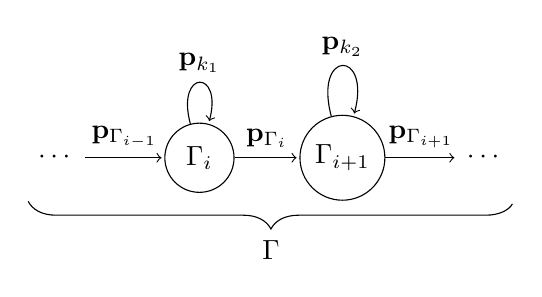
\begin{tikzpicture}[shorten >=1pt,node distance=12ex,on grid,auto] 
    \node        (q_dots0) {$\cdots$};
    \node[state] (q_0) [right=of q_dots0] {$\Gamma_i$};
    \node[state] (q_1) [right=of q_0] {$\Gamma_{i+1}$};
    \node        (q_dots1) [right=of q_1] {$\cdots$};   
    \path[->]
    (q_dots0) edge node{$\mathbf{p}_{\Gamma_{i-1}}$} (q_0)
    (q_0) edge node {$\mathbf{p}_{\Gamma_i}$} (q_1)    
    (q_0) edge [loop above] node {$\mathbf{p}_{k_1}$} (q_0)
    (q_1) edge node {$\mathbf{p}_{\Gamma_{i+1}}$} (q_dots1)
    (q_1) edge [loop above] node {$\mathbf{p}_{k_2}$} (q_1)
    ; %end path 
    \draw [decorate,decoration={brace,amplitude=10pt,mirror,raise=10pt},yshift=0pt]
    (q_dots0.south west) -- (q_dots1.south east) node [black,midway,yshift=-8ex]{$\Gamma$};
  \end{tikzpicture}
  \caption{The plan defined as a finite state machine}
  \label{fig:state-machine}
\end{figure}

A slice of the plan in Figure~\ref{fig:state-machine} shows the transition between the stages. The triggering point $\mathbf{p}_{\Gamma_{i-1}}$ allows the transition to stage $\Gamma_i$. The UAV remains in the stage with any generic point $\mathbf{p}_{k_1}$ and $\mathbf{p}_{k_2}$. It eventually enters the stage $\Gamma_{i+1}$ with the triggerint point $\mathbf{p}_{\Gamma_i}$ and so on, until it reaches the last triggering point.

Generally, one can express the triggering points in function of the $i$-th trajectory parameters $c_{i,1},\dots,c_{i,\rho}$, or any previous trajectory parameters, propagating the information therein if necessary. See Figure~\ref{fig:state-machine2} where, for simplicity, we neglected the $\sigma=0$ computations parameters, so $c_i=c_{i,1},\dots,c_{i,\rho}$.

\begin{figure}[h]
  \center
  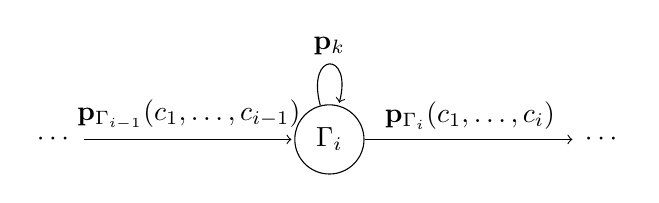
\begin{tikzpicture}[shorten >=1pt,node distance=23ex,on grid,auto] 
    \node        (q_dots0) {$\cdots$};
    \node[state] (q_0) [right=of q_dots0] {$\Gamma_i$};
    \node        (q_dots1) [right=of q_0] {$\cdots$};   
    \path[->]
    (q_dots0) edge node{$\mathbf{p}_{\Gamma_{i-1}}(c_1,\dots,c_{i-1})$} (q_0)
    (q_0) edge node {$\mathbf{p}_{\Gamma_i}(c_1,\dots,c_{i})$} (q_dots1)    
    (q_0) edge [loop above] node {$\mathbf{p}_{k}$} (q_0)
    ; %end path
  \end{tikzpicture}
  \caption{Detail of the stage $\Gamma_i$ in the finite state machine}
  \label{fig:state-machine2}
\end{figure}

We refer the reader to an example in Appendix~\ref{app:plan-example} for a detailed implementation. In the example, the first trajectory parameter is propagated to all the following trajectories and triggering points. 

We store the plan in the plan specification, the format is described in Appendix~\ref{app:plan-spec}. 


\section{Periodic Energy Model}
\label{sec:energy-model}

We model the energy using some energy coefficients $\mathbf{q}\in\mathbb{R}^m$ that characterize the energy signal. We refer to the instantaneous energy consumption evolution simply as the energy signal. The coefficients are derived from Fourier analysis (the size of the energy coefficients vector $m$ is related to the order of a Fourier series) and estimated using a state estimator (Kalman filter). 

We proof a relation between the energy signal and the energy coefficients in Theorem~\ref{thm:state-vs-energy}. We show after the main results how this approach allows us variability in terms of the systems behaving periodically, piece-wise periodically, or merely linearly with sporadic periodicity.

Once we illustrate the energy model, we enhance it with the energy contribution of the computations in Subsection~\ref{sec:computations-model}. 

Let us consider a periodic signal of period $T\in\mathbb{R}_{> 0}$, and a Fourier series of an arbitrary order $r\in\mathbb{Z}_{\geq 0}$ for the purpose of modeling of the signal
\begin{equation}\label{eq:fourier}
  h(t)=a_0/T+(2/T)\sum_{j=1}^{r}{\left(a_j\cos{\omega jt}+b_j\sin{\omega jt}\right)},
\end{equation}
where $h:\mathbb{R}_{\geq 0}\rightarrow\mathbb{R}$ maps time to the instantaneous energy consumption, $\omega:=2\pi/T$ is the angular frequency, and $a,b\in\mathbb{R}$ the Fourier series coefficients.

We use extensively the following assumption for the purpose of energy signal modeling.
\begin{assm}[Energy signal periodicity]\label{assm:periodic} 
Given two time instants $k_1,k_2$ s.t. $k_1>k_2$ and a constant value $n\in\mathbb{Z}_{> 0}$
\begin{equation*}
  \abs{y_{k}-y_{k+n}}\in\mathbb{E}\subset\mathbb{R}_{\geq 0} \,\,\,\forall k\in[k_1,k_2],
\end{equation*}
for a small enough set $\mathbb{E}$.
\end{assm}

Physically this means that the energy signal is assumed to be approximately periodic.

Let us consider a linear time-invariant (LTI) state-space model
\begin{equation}\label{eq:state-perf}\begin{split}
  \dot{\mathbf{q}}&=A\mathbf{q}+B\mathbf{u}+\mathbf{w},\\
  y&=C\mathbf{q}+v,
\end{split}\end{equation}
where $y\in\mathbb{R}_{\geq 0}$ is the instantaneous energy consumption, and $\mathbf{w}\in\mathbb{R}^m,v\in\mathbb{R}$ are the contributions of the uncertainty. 

The state $\mathbf{q}$ are the energy coefficients
\begin{equation}\label{eq:state-details}\begin{split}
  \mathbf{q}&=\left[\begin{array}{cccccc}
    \alpha_0 & \alpha_1 & \beta_1 & \cdots & \alpha_r & \beta_r
  \end{array}\right]^T,\\
  A&=\left[\begin{array}{cccc}
    0&    &       &  \\
     & A_1&       &  \\
     &    & \ddots&  \\
     &    &       & A_r 
  \end{array}\right],\,A_j\begin{bmatrix}0 & \omega j \\ -\omega j & 0\end{bmatrix},\\
  C&=(1/T)\left[\begin{array}{cccccc}
    1 & 1 & 0 &\cdots & 1 & 0
  \end{array}\right],
\end{split}\end{equation}
where $\mathbf{q}\in\mathbb{R}^m$ with $m=2r+1$, $A\in\mathbb{R}^{m\times m}$ is the state transmission matrix, and $C\in\mathbb{R}^m$ is the output matrix. In matrix $A$, the top left entry is zero, the diagonal entries are $A_1,\dots,A_r$, the remaining entries are zeros.

\begin{lem}[Signals equality]\label{lem:eqv}Suppose there is no state and output uncertainty (the contributions $\mathbf{w},v$ are zeros) and the control is zero. Suppose further matrices $A,C$ are described by Equation~(\ref{eq:state-details}), and the initial guess $\mathbf{q}_0$ is $\mathbf{q}_0=\begin{bmatrix}a_0 & a_1/2 & b_1/2 & \cdots & a_r/2 & b_r/2\end{bmatrix}$. Then, the signal $h$ in Equation~(\ref{eq:fourier}) is equal to the signal $y$ in Equation~(\ref{eq:state-perf}).
\end{lem}
\begin{proof}
The equivalence of the models is trivial and the equality of the two signals is achieved by a proper choice of items of matrices $A,C$ and the initial guess $\mathbf{q}_0$. We refer the reader to Appendix~\ref{app:proof-eqv} for a formal proof of the equality where we justify the choices of the items of the matrices and of the initial guess. 
\end{proof}

Let us consider the discretized version $A_d:=A\Delta t+I$ of the matrix $A$. We denote the continuous and discrete time with the standard notation $t,k$. We use the forward Euler approximation with a small enough value of the time step $\Delta t$. We note that one can guarantee to have the same outputs rather than an approximation with $A_d:=e^{At}$.

Let us suppose that at time instant $k$ the plan reached the $i$-th stage $\Gamma_i$.

The control along with the input matrix
\begin{equation}\label{eq:state-control}\begin{split}
  \mathbf{u}&=\begin{bmatrix}c_{i,1} & \cdots & c_{i,\rho} & c_{i,\rho+1} & \cdots & c_{i,\rho+\sigma}\end{bmatrix}^T,\\
  B\mathbf{u}&:=B_i(\mathbf{u}_k-\mathbf{u}_{k-1}),\,\,\,B_i=\left[\begin{array}{c} \nu_i\\\mathbf{0}\end{array}\right],
\end{split}\end{equation}
where $\mathbf{u}\in\mathbb{R}^n$ is the control with $n=\rho+\sigma$, $B\in\mathbb{R}^{m\times n}$, and $\mathbf{u}_{-1}=\mathbf{0}$. Moreover, the top row of $B$ contains gain factors $\nu_i=\begin{bmatrix}\nu_{i,1} & \cdots & \nu_{i,\rho} & \nu_{i,\rho + 1}& \cdots & \nu_{i,\rho+\sigma}\end{bmatrix}$, quantifying the contribution of a given parameter to the instantaneous energy consumption. The other entries of $B$ are zeros. 

The first $\rho$ gain factors quantifies the contribution of the $i$-th trajectory parameters. A first guess of these parameters is derived empirically. They are later refined by the algorithm. The following $\sigma$ gain factors quantifies the contribution of the computations parameters. They are derived using the modeling tool. We use the gain factors to select the optimal control $\mathbf{u}^0$. 

Equation~(\ref{eq:state-control}) accounts for the energy due to the change of parameters $\mathbf{u}_k-\mathbf{u}_{k-1}$. For instance, when the trajectory $\varphi_1$ is a circle (see Figure~\ref{fig:tee1}), a decrement in the trajectory parameter $c_{1,1}$--the radius of the circle--adds a negative contribution. It thus simulates the lowering of instantaneous energy consumption $\nu_{1,1}(c_{1,1}-c_{1,1}^-)<0$, for a given $\nu_{1,1}\in\mathbb{R}_{<0}$. 

\subsection{Trajectory parameters energy contribution}
\label{sec:model}

\begin{figure}[h]
  \centering
  
\definecolor{cDEDEDE}{RGB}{222,222,222}
\definecolor{c2B2B2B}{RGB}{43,43,43}
\definecolor{cFFFFFF}{RGB}{255,255,255}
\definecolor{c9B9B9B}{RGB}{155,155,155}
\definecolor{c989898}{RGB}{152,152,152}
\definecolor{c4D4D4D}{RGB}{77,77,77}


\def \globalscale {.870000}
\begin{tikzpicture}[y=0.80pt, x=0.80pt, yscale=-\globalscale, xscale=\globalscale, inner sep=0pt, outer sep=0pt]
\path[fill=cDEDEDE,line join=round,line width=1.280pt] (11.6098,143.2690) -- (11.6381,143.2690) .. controls (12.6918,105.8790) and (43.0061,75.8094) .. (80.4938,75.1490) -- (80.4938,111.5790) .. controls (63.0922,112.2190) and (49.0572,126.0420) .. (48.0821,143.3560) -- (48.0967,157.7040) -- (48.0821,158.0290) -- (48.0821,158.3590) .. controls (48.0975,159.1860) and (48.2166,160.0470) .. (48.1937,160.8610) -- (48.1998,160.8690) -- (48.1998,162.8820) -- (48.0821,208.4660) -- (48.0821,216.6680) -- (48.0610,216.6680) -- (48.0605,216.8310) -- (48.0484,217.7520) -- (48.1143,221.9450) -- (11.4101,221.9530) .. controls (11.4101,220.0520) and (11.3860,223.8120) .. (11.3745,219.6040) -- (11.3745,217.8520) -- (11.3745,217.4970) -- (11.3745,217.0210) -- (11.3745,216.6730) -- (11.3745,145.5000) -- (11.6098,143.2690) -- cycle;



\path[draw=c2B2B2B,line join=round,line width=0.512pt] (81.7300,145.1480) ellipse (1.9796cm and 1.9796cm);



\path[draw=black,line join=round,line width=0.512pt] (84.1885,147.4600) -- (79.3297,142.5950);



\path[draw=black,line join=round,line width=0.512pt] (79.3321,147.4590) -- (84.1972,142.5950);



\path[draw=c2B2B2B,line join=round,line width=0.512pt] (11.6130,57.9496) -- (11.6123,221.7820);



\path[draw=black,line join=round,line width=0.512pt] (81.8116,145.0640) -- (11.5289,145.0640);



\path[fill=black,line join=round,line width=0.256pt] (17.2158,147.6960) -- (17.2088,142.3370) -- (12.3038,145.0230) -- (17.2158,147.6960) -- cycle;



\path[draw=black,line join=round,line width=1.024pt] (86.9347,19.9572) .. controls (95.0742,22.1535) and (96.9997,30.5095) .. (96.9997,30.5095) .. controls (96.9997,30.5095) and (112.2540,68.0133) .. (71.9151,75.7553) .. controls (66.6769,76.7607) and (67.8409,77.7130) .. (70.6628,77.6073);



\path[draw=black,fill=cFFFFFF,line join=round,line width=0.512pt] (103.4020,39.3713) -- (99.4578,23.0489) -- (95.8475,27.2484) -- (90.3755,28.7747) -- (103.4020,39.3713) -- cycle;



  \path[fill=cFFFFFF,line join=round,line width=1.024pt,rounded corners=0.0000cm] (4.7286,68.9128) rectangle (18.8758,87.0599);



  \path[cm={{1.0,0.0,0.0,1.0,(3.0,83.0)}}] (0.0000,0.0000) node[above right] () {$\varphi_2$};



  \path[fill=cFFFFFF,line join=round,line width=1.024pt,rounded corners=0.0000cm] (100.3810,72.5529) rectangle (118.5282,86.7001);



  \path[cm={{1.0,0.0,0.0,1.0,(102.0,86.0)}}] (0.0000,0.0000) node[above right] () {$\varphi_1$};



  \path[fill=cFFFFFF,line join=round,line width=1.024pt] (55.4211,215.8850) -- (41.2739,215.8850) -- (41.2532,229.5530) -- (55.4334,229.5530) -- (55.4211,215.8850) -- cycle;



  \path[cm={{1.0,0.0,0.0,1.0,(44.0,228.0)}}] (0.0000,0.0000) node[above right] () {$\underline{c}_1$};



  \path[fill=cFFFFFF,line join=round,line width=1.024pt] (69.0222,142.0810) -- (48.8751,142.0800) -- (48.8751,156.2270) -- (69.0222,156.2280) -- (69.0222,142.0810) -- cycle;



  \path[cm={{1.0,0.0,0.0,1.0,(50.0,156.0)}}] (0.0000,0.0000) node[above right] () {$c_{1,1}$};



\path[line join=round,line width=1.280pt] (96.2907,30.0560) -- (102.5890,72.8363);



\path[draw=black,line join=round,line width=0.512pt] (97.7561,30.2009) -- (87.0057,56.4820);



\path[draw=black,line join=round,line width=0.512pt] (97.6471,30.4476) -- (102.6580,4.6067);



\path[draw=black,line join=round,line width=0.512pt] (97.7199,30.4068) -- (117.4940,50.2130);



\path[cm={{1.0,0.0,0.0,1.0,(109.0,10.0)}}] (0.0000,0.0000) node[above right] () {$\nabla\varPhi$};



\path[cm={{1.0,0.0,0.0,1.0,(124.0,54.0)}}] (0.0000,0.0000) node[above right] () {$\dot{\mathbf{p}}$};



\path[cm={{1.0,0.0,0.0,1.0,(64.0,58.0)}}] (0.0000,0.0000) node[above right] () {$\dot{\mathbf{p}}_d$};



\path[fill=black,line join=round,line width=0.256pt] (11.3215,210.9780) -- (11.3443,205.6440) -- (12.6243,205.6500) -- (12.6015,210.9830) -- (11.3215,210.9780) -- cycle(11.3670,200.3110) -- (11.3898,194.9780) -- (12.6698,194.9830) -- (12.6470,200.3160) -- (11.3670,200.3110) -- cycle(11.4126,189.6440) -- (11.4353,184.3110) -- (12.7153,184.3170) -- (12.6925,189.6500) -- (11.4126,189.6440) -- cycle(11.4581,178.9780) -- (11.4808,173.6450) -- (12.7608,173.6500) -- (12.7381,178.9830) -- (11.4581,178.9780) -- cycle(11.5036,168.3110) -- (11.5264,162.9780) -- (12.8063,162.9830) -- (12.7836,168.3170) -- (11.5036,168.3110) -- cycle(11.5491,157.6450) -- (11.5719,152.3110) -- (12.8519,152.3170) -- (12.8291,157.6500) -- (11.5491,157.6450) -- cycle(11.5946,146.9780) -- (11.6174,141.6450) -- (12.8974,141.6500) -- (12.8746,146.9840) -- (11.5946,146.9780) -- cycle(11.6402,136.3120) -- (11.6456,135.0380) -- (11.6568,134.9130) -- (11.6932,134.7930) -- (11.7530,134.6830) -- (11.8340,134.5870) -- (11.9300,134.5070) -- (12.0405,134.4480) -- (12.1606,134.4120) -- (12.2856,134.4010) -- (11.7546,134.3300) -- (12.0956,132.6080) -- (12.4947,130.9340) -- (13.7459,131.2040) -- (13.3469,132.8780) -- (13.0149,134.5540) -- (12.2856,135.6810) -- (12.9256,135.0440) -- (12.9201,136.3170) -- (11.6402,136.3120) -- cycle(13.9627,125.7500) -- (15.1381,122.2860) -- (15.7773,120.7010) -- (16.9782,121.1440) -- (16.3390,122.7300) -- (15.1854,126.1290) -- (13.9627,125.7500) -- cycle(17.9048,115.7710) -- (19.4398,112.5680) -- (20.3445,110.9840) -- (21.4793,111.5760) -- (20.5746,113.1600) -- (19.0771,116.2850) -- (17.9048,115.7710) -- cycle(23.0920,106.3590) -- (26.1148,101.9430) -- (26.1387,101.9140) -- (27.1624,102.6830) -- (27.1385,102.7120) -- (24.1782,107.0360) -- (23.0920,106.3590) -- cycle(29.5404,97.8067) -- (30.4915,96.6583) -- (33.2732,93.9193) -- (34.2182,94.7827) -- (31.4365,97.5218) -- (30.5641,98.5752) -- (29.5404,97.8067) -- cycle(37.2744,90.3026) -- (41.4654,87.0041) -- (42.3134,87.9630) -- (38.1224,91.2613) -- (37.2744,90.3026) -- cycle(46.0669,84.1674) -- (48.4869,82.6899) -- (50.8339,81.6290) -- (51.4336,82.7599) -- (49.0866,83.8208) -- (46.7993,85.2173) -- (46.0669,84.1674) -- cycle(55.6938,79.4321) -- (56.2989,79.1584) -- (60.8364,77.7568) -- (61.2906,78.9536) -- (56.7531,80.3552) -- (56.2934,80.5630) -- (55.6938,79.4321) -- cycle(66.0352,76.2711) -- (71.2852,75.3315) -- (71.5875,76.5753) -- (66.3376,77.5149) -- (66.0352,76.2711) -- cycle(11.2760,221.6440) -- (11.2988,216.3110) -- (12.5788,216.3160) -- (12.5560,221.6500) -- (11.2760,221.6440) -- cycle;



  \path[fill=cFFFFFF,line join=round,line width=1.024pt] (17.0292,215.8850) -- (2.8821,215.8850) -- (2.8439,229.6060) -- (17.0241,229.5710) -- (17.0292,215.8850) -- cycle;



  \path[cm={{1.0,0.0,0.0,1.0,(0.0,228.0)}}] (0.0000,0.0000) node[above right] () {$\overline{c}_1$};



\path[draw=black,fill=c9B9B9B,line join=round,line width=0.512pt] (61.6373,78.2313) -- (78.4070,79.1025) -- (74.0128,75.1019) -- (75.5070,68.7650) -- (61.6373,78.2313) -- cycle;



\path[cm={{1.0,0.0,0.0,1.0,(44.0,74.0)}}] (0.0000,0.0000) node[above right] () {$\mathbf{q}_{k_2}$};



\path[draw=black,line join=round,line width=0.512pt] (16.6794,16.7674) -- (16.6794,42.6379);



\path[draw=black,line join=round,line width=0.512pt] (42.3726,42.4284) -- (16.5020,42.4284);



\path[cm={{1.0,0.0,0.0,1.0,(3.0,56.0)}}] (0.0000,0.0000) node[above right] () {$\mathcal{O}_W$};



\path[draw=black,line join=round,line width=0.512pt] (16.7257,42.3088) -- (97.1806,30.4695);



  \path[fill=cFFFFFF,line join=round,line width=1.024pt,rounded corners=0.0000cm] (49.9754,26.6677) rectangle (72.1225,40.8148);



  \path[cm={{1.0,0.0,0.0,1.0,(52.0,39.0)}}] (0.0000,0.0000) node[above right] () {$\mathbf{p}_{k_1}$};



\path[draw=black,line join=round,line width=0.512pt] (38.6977,10.4359) -- (58.2164,10.4359);



\path[cm={{1.0,0.0,0.0,1.0,(41.0,7.0)}}] (0.0000,0.0000) node[above right] () {$w$};



\path[draw=black,line join=round,line width=0.512pt] (62.0076,78.1286) -- (73.9018,75.1006);



\path[draw=black,line join=round,line width=0.512pt] (95.8349,27.2494) -- (103.2960,39.2649);



\path[fill=cDEDEDE,line join=round,even odd rule,line width=1.280pt] (224.1960,79.0527) .. controls (230.8220,76.8331) and (237.6090,75.2867) .. (244.9510,75.1573) -- (244.9510,111.5880) .. controls (227.5490,112.2270) and (213.5140,126.0500) .. (212.5390,143.3640) -- (212.5540,157.7130) -- (212.5390,158.0380) -- (212.5390,158.3670) .. controls (212.5540,159.1950) and (212.6730,160.0560) .. (212.6510,160.8690) -- (212.6570,160.8770) -- (212.6570,162.8900) -- (212.5390,208.4750) -- (212.5390,216.6770) -- (212.5180,216.6770) -- (212.5170,216.8390) -- (212.5050,217.7600) -- (212.5710,221.9540) -- (192.3530,221.9580) .. controls (192.6700,199.1980) and (191.5340,166.8170) .. (192.5090,145.6400) .. controls (192.9850,135.2980) and (195.2800,127.3770) .. (195.9520,125.0400) .. controls (198.4750,116.2690) and (196.6740,90.4278) .. (223.6900,79.2456) -- (224.1960,79.0527) -- cycle;



\path[draw=c989898,line join=round,line width=0.512pt] (246.1920,145.1650) ellipse (1.9796cm and 1.9796cm);



\path[draw=black,line join=round,line width=0.512pt] (248.6570,147.4780) -- (243.7920,142.6130);



\path[draw=black,line join=round,line width=0.512pt] (243.7940,147.4760) -- (248.6590,142.6110);



\path[draw=c2B2B2B,line join=round,line width=0.512pt] (246.8040,145.4130) ellipse (1.5285cm and 1.5285cm);



\path[draw=c4D4D4D,line join=round,line width=0.512pt] (192.6100,57.9662) -- (192.6090,221.7990);



\path[draw=black,line join=round,line width=0.512pt] (296.9870,164.5190) -- (246.4180,145.1250);



\path[draw=black,line join=round,line width=1.024pt] (251.3970,19.9740) .. controls (259.5360,22.1703) and (261.4620,30.5262) .. (261.4620,30.5262) .. controls (261.4620,30.5262) and (276.8830,68.0926) .. (236.4940,75.5674) .. controls (196.1050,83.0422) and (198.8250,115.0770) .. (195.9570,125.0480) .. controls (192.9930,135.3560) and (192.5400,144.9810) .. (192.5400,144.9810) -- (192.5560,145.2830) -- (192.6030,145.7910);



\path[draw=black,fill=cFFFFFF,line join=round,line width=0.512pt] (267.8640,39.3875) -- (263.9200,23.0652) -- (260.3100,27.2647) -- (254.8380,28.7911) -- (267.8640,39.3875) -- cycle;



\path[draw=black,fill=c9B9B9B,line join=round,line width=0.512pt] (193.0920,137.5170) -- (202.1750,123.3930) -- (196.2420,124.2600) -- (191.7620,120.7770) -- (193.0920,137.5170) -- cycle;



\path[fill=black,line join=round,line width=0.256pt] (191.9100,211.5420) -- (191.9100,206.2080) -- (193.1900,206.2080) -- (193.1900,211.5420) -- (191.9100,211.5420) -- cycle(191.9100,200.8750) -- (191.9100,195.5420) -- (193.1900,195.5420) -- (193.1900,200.8750) -- (191.9100,200.8750) -- cycle(191.9100,190.2080) -- (191.9100,184.8750) -- (193.1900,184.8750) -- (193.1900,190.2080) -- (191.9100,190.2080) -- cycle(191.9100,179.5420) -- (191.9100,174.2080) -- (193.1900,174.2080) -- (193.1900,179.5420) -- (191.9100,179.5420) -- cycle(191.9100,168.8750) -- (191.9100,163.5420) -- (193.1900,163.5420) -- (193.1900,168.8750) -- (191.9100,168.8750) -- cycle(191.9100,158.2080) -- (191.9100,152.8750) -- (193.1900,152.8750) -- (193.1900,158.2080) -- (191.9100,158.2080) -- cycle(191.9100,147.5420) -- (191.9100,145.4240) -- (193.1900,145.4240) -- (193.1900,147.5420) -- (191.9100,147.5420) -- cycle(191.9100,222.2080) -- (191.9100,216.8750) -- (193.1900,216.8750) -- (193.1900,222.2080) -- (191.9100,222.2080) -- cycle;



  \path[fill=cFFFFFF,line join=round,line width=1.024pt,rounded corners=0.0000cm] (185.7260,68.9295) rectangle (199.8732,87.0767);



  \path[cm={{1.0,0.0,0.0,1.0,(184.0,83.0)}}] (0.0000,0.0000) node[above right] () {$\varphi_2$};



  \path[fill=cFFFFFF,line join=round,line width=1.024pt] (197.3250,215.8840) -- (183.1780,215.8840) -- (183.1390,229.6050) -- (197.3200,229.5700) -- (197.3250,215.8840) -- cycle;



  \path[cm={{1.0,0.0,0.0,1.0,(180.0,230.0)}}] (0.0000,0.0000) node[above right] () {$\overline{c}_1^-$};



  \path[fill=cFFFFFF,line join=round,line width=1.024pt,rounded corners=0.0000cm] (257.2650,146.4430) rectangle (281.4121,164.5902);



  \path[cm={{1.0,0.0,0.0,1.0,(259.0,160.0)}}] (0.0000,0.0000) node[above right] () {$c_{1,1}^-$};



\path[line join=round,line width=1.280pt] (260.7530,30.0728) -- (267.0510,72.8529);



\path[draw=black,fill=cFFFFFF,line join=round,line width=0.512pt] (226.1000,78.2477) -- (242.8690,79.1187) -- (238.4750,75.1181) -- (239.9690,68.7813) -- (226.1000,78.2477) -- cycle;



  \path[fill=cFFFFFF,line join=round,line width=1.024pt] (222.2130,114.2280) -- (204.0660,114.2280) -- (204.0660,132.3750) -- (222.2130,132.3750) -- (222.2130,114.2280) -- cycle;



  \path[cm={{1.0,0.0,0.0,1.0,(206.0,129.0)}}] (0.0000,0.0000) node[above right] () {$\mathbf{q}_{k_3}$};



  \path[fill=cFFFFFF,line join=round,line width=1.024pt,rounded corners=0.0000cm] (214.1760,59.6814) rectangle (228.3232,73.8285);



  \path[cm={{1.0,0.0,0.0,1.0,(217.0,69.0)}}] (0.0000,0.0000) node[above right] () {$\mathbf{p}_{k_2}$};



\path[draw=black,line join=round,line width=0.512pt] (226.4700,78.1454) -- (238.3640,75.1173);



\path[draw=black,line join=round,line width=0.512pt] (193.2910,136.7850) -- (196.1980,124.3340);



\path[draw=black,line join=round,line width=0.512pt] (260.2970,27.2662) -- (267.7580,39.2815);



  \path[fill=cFFFFFF,line join=round,line width=1.024pt] (244.6550,186.5990) -- (226.5070,186.6000) -- (226.5070,204.7470) -- (244.6550,204.7460) -- (244.6550,186.5990) -- cycle;



  \path[cm={{1.0,0.0,0.0,1.0,(229.0,201.0)}}] (0.0000,0.0000) node[above right] () {$\varphi_1$};



\path[draw=c989898,line join=round,line width=0.512pt] (176.0540,57.9854) -- (176.0540,221.8180);



\path[cm={{1.0,0.0,0.0,1.0,(40.0,242.0)}}] (0.0000,0.0000) node[above right] () {\footnotesize (a) initial path};



\path[cm={{1.0,0.0,0.0,1.0,(201.0,242.0)}}] (0.0000,0.0000) node[above right] () {\footnotesize (b) path adjustment};



\path[fill=black,line join=round,line width=0.256pt] (293.9350,160.3200) -- (291.8540,165.2580) -- (297.4170,164.6960) -- (293.9350,160.3200) -- cycle;



\path[fill=black,line join=round,line width=0.256pt] (40.6563,39.7237) -- (40.6634,45.0822) -- (45.5684,42.3968) -- (40.6563,39.7237) -- cycle;



\path[fill=black,line join=round,line width=0.256pt] (14.0109,18.2453) -- (19.3694,18.2414) -- (16.6871,13.3348) -- (14.0109,18.2453) -- cycle;



\path[fill=black,line join=round,line width=0.256pt] (116.9490,45.7122) -- (113.0620,49.4016) -- (118.3850,51.1170) -- (116.9490,45.7122) -- cycle;



\path[fill=black,line join=round,line width=0.256pt] (99.7091,6.2037) -- (104.9810,7.1609) -- (103.2230,1.8527) -- (99.7091,6.2037) -- cycle;



\path[fill=black,line join=round,line width=0.256pt] (85.7351,59.6833) -- (89.9853,56.4200) -- (84.8713,54.1581) -- (85.7351,59.6833) -- cycle;



\path[fill=black,line join=round,line width=0.256pt] (57.4367,7.5138) -- (57.4438,12.8723) -- (62.3487,10.1869) -- (57.4367,7.5138) -- cycle;



\path[fill=black,line join=round,line width=0.256pt] (92.5154,28.4558) -- (93.3888,33.7428) -- (97.7950,30.2997) -- (92.5154,28.4558) -- cycle;




\end{tikzpicture}


  \caption{Illustrative example of the alteration of a trajectory parameter}
  \label{fig:tee1}
\end{figure}

Let us assume that the set
\begin{equation}\label{eq:area}
  \mathcal{P}_i:=\{\mathbf{p}_k\mid\varphi_i(\mathbf{p}_k,c_{i,1},\dots,c_{i,\rho})\in\mathbb{C}_i\},
\end{equation}
delimits the area where the $i$-th trajectory $\varphi_i$ is free to evolve using the trajectory parameters $c_{i,1},...,c_{i,\rho}$ (the gray area in Figure~\ref{fig:tee1}). $\varphi_i$ is a function of the two coordinates and is equal to zero when a point $\mathbf{p}_k$ is on the trajectory. Physically, this means the UAV is flying exactly over the nominal trajectory. The trajectory parameters allows to change the trajectory. They are a way to alter the nominal trajectory in the initial plan and thus alter the energy signal.
In fact, the algorithm uses the set from Equation~(\ref{eq:area}) to alter the optimal trajectory parameters $c_i^0$ (here we again neglect for simplicity the $\sigma=0$ computations parameters), such that $\varphi_i(\mathbf{p}_k,c_i^0)$ has the highest instantaneous energy consumption (while still respecting the energy budget). 

We derive the new position $\mathbf{p}_{k+1}$ using the function $\varPhi:=\varphi_i(\mathbf{p}_k,\mathbf{c}_i^0)$, computing its vector field $\nabla\varPhi:=\begin{bmatrix}\partial\varPhi/\partial x & \partial\varPhi/\partial y\end{bmatrix}^T$, and the direction to follow in the form of velocity vector~\cite{de2017guidance}
\begin{equation}\label{eq:pd}
  \dot{\mathbf{p}}_d(\mathbf{p}_k):=E\nabla\varPhi-k_e\varPhi\nabla\varPhi,\,\,\,E=\begin{bmatrix}
    0&1\\-1&0
  \end{bmatrix},
\end{equation}
where $E$ specifies the rotation (which influence the tracking direction), and $k_e\in\mathbb{R}_{\geq 0}$ the gain to adjusts the speed of convergence. The direction the velocity vector $\dot{\mathbf{p}}_d$ is pointing at is generally different from the course heading due to the uncertainty, such as wind ($w\in\mathbb{R}$ in Figure~\ref{fig:tee1}).

\subsection{Computations parameters energy contribution}
\label{sec:computations-model}

Let us recall from Definition~\ref{def:mission} that the $i$-th stage $\Gamma_i$ of the plan $\Gamma$ contains the computations parameters which characterize the computations. We assess the energy cost of these computations using \powprof{}, the open-source modeling tool adapted from earlier work on computational energy analysis~\cite{seewald2019coarse, seewald2019component}, and energy estimation of a fixed-wing UAV~\cite{seewald2020mechanical}. 

We assume the UAV carries an embedded board that runs the computations. The tool measures the instantaneous energy consumption of a subset of possible computations parameters within the computations constraints sets and builds an energy model: a linear interpolation, one per each computation. 

Specifically, the computations are implemented by software components, such as ROS nodes in a ROS based system. The user implements these nodes s.t. they change the computational load by node-specific ROS parameters--the computations parameters. In a generic software component system, the user maps the computational load to the arguments. In both cases, with ROS~\cite{zamanakos2020energy} or with generic software components system~\cite{seewald2019component}, the tool performs automatic modeling. For instance, if the computation is a CNN object detector, the computation parameter $c_{i,\rho+1}$ corresponds frames-per-second (fps) rate and the tool changes the detection frequency to build a model. The model is then a linear multivariate interpolation for all the parameters.

We note that while the trajectory can differ for each stage, the tasks remain the same. However, the user can inhibit or enable a computation varying its computation set.

Let us further define $g:\mathbb{Z}_{\geq 0}\rightarrow\mathbb{R}_{\geq 0}$ as the instantaneous computational energy consumption value obtained using the tool.

The gain factors that quantifies the contribution of the computations parameters
\begin{equation}\label{eq:energy-comp}
  \begin{bmatrix}\nu_{i,\rho+1} \\ \vdots \\ \nu_{i,\rho+\sigma}\end{bmatrix}^T=\begin{bmatrix}g(c_{i,\rho+1}) \\ \vdots \\ g(c_{i,\rho+\sigma})\end{bmatrix}/\begin{bmatrix}c_{i,\rho+1} & \cdots & c_{i,\rho+\sigma}\end{bmatrix}.
\end{equation}
Moreover, let $g(\{\emptyset\})$ be zero.

\leavevmode\thispagestyle{empty}\newpage


%%%%%%%%%%%%%%%%%%%
\section{Algorithm}
\label{sec:algo}

Given $l$ stages $\mathcal{M}_i$ (TEE $\varphi_i$, tasks $\Psi$, computations $\mathbf{s}_i\in\mathbb{S}_i$, and adaptations $\mathbf{c}_i\in\mathbb{C}_i$ for all $i\in[l]$), the main purpose of the algorithm is to output a control input sequence $\mathbf{u}^a:=\{\mathbf{u}_0^a,\mathbf{u}_1^a,\dots\}$ in a valid mission.

\begin{defn}[Valid mission]\label{def:valid}
  A mission is valid if for every stage $\mathcal{M}_{i-1},\,i\in[l]^+$ there exist a control input $\mathbf{u}_k^{a}$ that produce the next stage $\mathcal{M}_i$
  \begin{equation}\begin{split}\label{eq:mission-valid}
    \mathbf{u}^a_{k}=\{&\langle\mathbf{c}_{k},\mathbf{s}_{k}\rangle\mid\,\exists n\in\mathbb{Z}_{>0},\\&\langle\varphi_{i-1}(\mathbf{p}_{k-n},\mathbf{c}_{k-n}),\Psi(\mathbf{s}_{k-n})\rangle\in\mathcal{M}_{i-1}\\
    &\Longrightarrow\langle\varphi_i(\mathbf{p}_{k},\mathbf{c}_{k}),\Psi(\mathbf{s}_{k})\rangle\in\mathcal{M}_{i}\}.
  \end{split}\end{equation}
\end{defn}

Let us proof that if the mission is valid, the instantaneous energy consumption can be modeled as linear combination of the state from the Equation~(\ref{eq:state-perf}).

\begin{thm}[Periodic energy model]\label{thm:state-vs-energy}
  Consider the mission from Definition~\ref{def:mission}, the valid mission from~\ref{def:valid}. Assume Assumption~\ref{assm:periodic} holds, the model of Equation~(\ref{eq:state-perf}) behaves ideally ($\mathbf{w}=\mathbf{0},v=0$), the initial energy coefficients state $\mathbf{q}_0$ is $y_0^a/m$ for the first coefficient where $y_0^a\in\mathbb{R}_{>0}$ is an initial measurement\footnote{$y_0^a$ can be the initial measurement or the measurement from a previous instance of the algorithm}, $(1/2)y_0^a/m$ for all the others, and the mission is valid.
  Then, the instantaneous energy consumption $y_k$ is a linear combination of the state $\mathbf{q}_k$.
\end{thm}
\begin{proof}
  The proof is based on mathematical induction. 
  Base case: we proof that $y_0=y_0^a$. Recall the definition of the state in Equation~(\ref{eq:state-details}). The output is $y_{0}=\alpha_{0,0}+\alpha_{0,1}+\dots+\alpha_{0,r}=y_0^a/m+(1/2)y_0^a/m+\cdots+(1/2)y_0^a/m=y_0^a$.
  
  Induction step: by inspection of Equation~(\ref{eq:state-perf}), the output at instant $k$ can be expressed $y_{k}=(\alpha_{0,0}+B\mathbf{u}_0+\dots+B\mathbf{u}_{k-1})+p_1(k)\alpha_{0,1}+\dots+p_r(k)\alpha_{0,r}$, where $\forall t\in\mathbb{Z}_{\geq 2}$
  \begin{equation}\label{eq:proof-pr}
    p_r(t):=\begin{cases}
      \prod_{i=1}^{t/2}{r^3/\xi^3}&\text{ for even }t\\
      (r/\xi)\prod_{i=1}^{(t-1)/2}{r^3/\xi^3}&\text{ for odd }t
    \end{cases}.
  \end{equation}
  
  Suppose $k$ is even and the theorem holds up to $k$. Initial energy coefficients state $\mathbf{q}_0$ leads to $y_{k}=(y_0^a/m+B\mathbf{u}_0+\dots+B\mathbf{u}_{k-1})+p_1(k)(1/2)y_0^a/m+\dots+p_r(k)(1/2)y_0^a/m=y_{k}^a$. 
  
  We prove now that the instantaneous energy consumption at $k+1$ is still a linear combination of the state. We express the output in function of the previous state $y_{k+1}=(\alpha_{0,0}+B\mathbf{u}_0+\dots+B\mathbf{u}_{k})+(1/\xi)\beta_{k,1}+\dots+(r/\xi)\beta_{k,r}$. Notice that the coefficients $\alpha,\beta$ have an equivalent evolution (indeed this allows to simulate the periodicity) and $\beta_{k,r}=p_r(k)\beta_{0,r}$. Thus, the output can be expressed $y_{k+1}=(\alpha_{0,0}+B\mathbf{u}_0+\dots+B\mathbf{u}_{k})+(1/\xi)p_1(k)\beta_{0,1}+\dots+(r/\xi)p_r(k)\beta_{0,r}$. The expression is equivalent to $y_{k+1}=(\alpha_{0,0}+B\mathbf{u}_0+\dots+B\mathbf{u}_{k})+p_r(k+1)\beta_{0,r}+\dots+p_r(k+1)\beta_{0,r}$ using the definition of $p_r$ in Equation~(\ref{eq:proof-pr}). Again, the state $\mathbf{q}_0$ leads to $y_{k+1}=(y_0^a/m+B\mathbf{u}_0+\dots+B\mathbf{u}_{k})+p_r(k+1)(1/2)y_0^a/m+\dots+p_r(k+1)(1/2)y_0^a/m=y_{k+1}^a$, alike the previous statement, but at instant $k+1$. The proof for odd $k$ is equivalent.
\end{proof}

\subsection{Output constraints set}

We stated earlier the output $y_k$--the instantaneous energy consumption--evolves in $\mathbb{R}_{\geq 0}$. This is generally untrue. Physical UAVs are bounded by strict energy budgets due to battery limitations.

Let us hence consider the state of charge (SoC) of such battery with a simplistic difference equation~\cite{seewald2020mechanical}
\begin{equation}\begin{split}
  \mathrm{SoC}_k=-\left(V-
  \sqrt{
    V^2-
    4R_r\tilde{V}y_kV^{-1}}
  \right)/2R_rQ_c,\\ 
\end{split}\end{equation}
where $V\in\mathbb{R}$ is the internal battery and $\tilde{V}\in\mathbb{R}$ the stabilized voltage, $R_r\in\mathbb{R}$ the resistance, and $Q_c\in\mathbb{R}$ the constant nominal capacity. We define the output constraints set
\begin{equation}
  \mathbb{Y}_k:=\{y_k\mid y_k\in[0,\mathrm{SoC}_kQ_cV]\subseteq{\mathbb{R}_{\geq 0}}\},
\end{equation}
and $\max{\mathbb{Y}}_k$ is the maximum discharge capacity by the internal battery voltage--the maximum instantaneous energy consumption.

\subsection{Deployment algorithm}

\begin{algorithmic}[1]
  \Procedure{Step}{$\mathbf{q}_{k-1}$, $\mathbf{u}_{k-1}^a$, $\mathbf{u}_{k-2}^a$, $P_{k-1}$}\label{alg:step}
  
  \State $\mathbf{u}_{k-1}\gets {\mathbf{u}_{k-1}(\max{\mathbf{u}}_{k-1}^a,\mathbf{u}_{k-2}^a)}$\label{alg:max_cont_sequence}

  \State $\mathbf{u}^0_{k-1}\gets\argmax_{\mathbf{u}}{\sum_{i=k-1}^{k+N-2}{l(\mathbf{q}_i,\mathbf{u}_i)+V_f(\mathbf{q}_{k+N-1})}}$\label{alg:mpc}

  \State $\hat{\mathbf{q}}_k^-\gets A\hat{\mathbf{q}}_{k-1} + B\mathbf{u}^0_{k-1}$
  \If{$C\hat{\mathbf{q}}_k^-\notin\mathbb{Y}_k$}\label{alg:output_constraints}
    \State $\mathbf{u}^a_{k-1}\gets\mathbf{u}^a_{k-1}/\{\max{\mathbf{u}}^a_{k-1}\}$
    \State\Return{\Call{Step}{$\mathbf{q}_{k-1}$, $\mathbf{u}^a_{k-1}$, $\mathbf{u}_{k-2}^a$,$P_{k-1}$}}\label{alg:recursion}
  \Else
    \If{$\abs{y_k^a-C\hat{\mathbf{q}}_k^-}\leq \varepsilon$}
      \State $\hat{\mathbf{q}}_k\gets\hat{\mathbf{q}}_k^-$\label{alg:evolution}
      \State $P_k\gets P_k^-$
    \Else 
      \State $P_k^-\gets AP_{k-1}A^T+Q$\label{alg:kalman_start}
      \State $K\gets P_k^-C^T/(CP_k^-C^T+R)$
      \State $\hat{\mathbf{q}}_k\gets \hat{\mathbf{q}}_k^-+K(y_k^a-C\hat{\mathbf{q}}_k^-)$
      \State $P_k\gets(I+KC)P_k^-$\label{alg:kalman_end}
    \EndIf
    \State $\mathbf{u}_{k}^a\gets \mathbf{u}_{k-1}^a$
    \State\Return{$(\hat{\mathbf{q}}_k,P_k,\mathbf{u}_k^a)$}
  \EndIf
  \EndProcedure
\vspace*{1ex}
  \Procedure{EADMPA}{$\mathcal{M}$, $\mathbf{p}_0$, $\mathbf{q}_0$}
  \State $k\gets 0$
%  \State $\mathbf{y}\gets \{\emptyset\}$
  \State $\mathbf{u}_{k-1}^a\gets\{\emptyset\}$
  \State $\mathbf{p}_k\gets\mathbf{p}_0$
  \State $\mathbf{q}_k\gets\mathbf{q}_0$
  \While{$k \leq t_f$}
    
    \State $\mathbf{u}_{k}^a\gets \{\mathbf{u}_{k}^a\mid(\varphi_i(\mathbf{p}_{k},\mathbf{c}_{i}),\Psi(\mathbf{s_{i}}))\in\lambda(\mathbf{p}_k)\}$
    \State $(\mathbf{q}_k,P_k,\mathbf{u}_k^a)\gets$\Call{Step}{$\mathbf{q}_{k}$, $\mathbf{u}^a_{k}$, $\mathbf{u}_{k-1}^a$, $P_k$}\label{alg:en}
    \State $\mathbf{p}_{k}\gets\mathbf{p}_k\dot{\mathbf{p}}_d(\mathbf{p}_k)/v$\label{alg:pos}
    \State $\mathbf{u}_{k-1}^a\gets\mathbf{u}_{k}^a$

%    \State $\mathbf{y}\gets\mathbf{y}\cup C\hat{\mathbf{q}}_k$
    \State $k\gets k + 1$
  \EndWhile 
  \EndProcedure
\end{algorithmic}

Per each time step $k$ (the final time $t_f$ is unknown), the algorithm updates the state--the position at line~\ref{alg:pos} and the energy coefficients at line~\ref{alg:en}--and the control input. Note that the position can be computed directly from Equation~(\ref{eq:pd}). If the velocity is $v\in\mathbb{R}_{\geq 0}$, and the starting point $\mathbf{p}_0$, $\mathbf{p}_{k+1}=\mathbf{p}_k\dot{\mathbf{p}}_d(\mathbf{p}_k)/v$.
  
In detail, initial guess for $P_0\in\mathbb{R}^{j\times j}$ is positive definite and derived empirically, for $\mathbf{q}_0$ the initial measurement is distributed to the coefficients (see Theorem~\ref{thm:state-vs-energy}). Line~\ref{alg:max_cont_sequence} selects the maximum possible control from the current control input. Line~\ref{alg:mpc} uses robust output feedback model predictive control (MPC)~\cite{rawlings2017model} to select the optimal control $\mathbf{u}^0$ for a given horizon $N\in\mathbb{Z}_{>0}$ from the cost function
\begin{equation}\begin{split}
  l(\mathbf{q}_k,\mathbf{u}_k)&:=(1/2)(\mathbf{q}_k^TQ\mathbf{q}_k+\mathbf{u}_k^TR\mathbf{u}_k),\\
  V_f(\mathbf{q}_k)&:=(1/2)(\mathbf{q}_k^TP_f\mathbf{q}_k),
\end{split}\end{equation}
where matrices $Q\in\mathbb{R}^{j\times j},R\in\mathbb{R}^{l\times l}$ are positive definite.

Follows a check if the mission can finish without the eventuality of battery discharge (output constraints satisfaction) at line~\ref{alg:output_constraints}, with the control input being eventually updated and the process reiterated at line~\ref{alg:recursion}.

Before the next step, state estimator--the discrete-time Kalman filter~\cite{simon2006optimal} at lines~\ref{alg:kalman_start}--\ref{alg:kalman_end}--predicts the state $\mathbf{q}$ if the modeled instantaneous energy consumption diverges from the sensor's value $y_k^a$ more than a given $\varepsilon\in\mathbb{R}_{\geq  0}$, or sensor measurements are unavailable ($y_k^a=0$).


%%%%%%%%%%%%%%%%%%%%
\section{Results}
\label{sec:experimental}

Some preliminary results are discussed. Further analysis and re-implementation of the functionality of the algorithm is needed.

\begin{figure}[h]
  \centering
  
\definecolor{c808080}{RGB}{128,128,128}


\def \globalscale {1.000000}
\begin{tikzpicture}[y=0.80pt, x=0.80pt, yscale=-\globalscale, xscale=\globalscale, inner sep=0pt, outer sep=0pt]
\begin{scope}[draw=black,line join=bevel,line cap=rect,even odd rule,line width=0.800pt]
  \begin{scope}[cm={{1.0,0.0,0.0,1.0,(0.0,0.0)}},draw=black,line join=bevel,line cap=rect,line width=0.800pt]
  \end{scope}
  \begin{scope}[cm={{1.00714,0.0,0.0,1.00714,(0.0,0.0)}},draw=black,line join=bevel,line cap=rect,line width=0.800pt]
  \end{scope}
  \begin{scope}[cm={{1.00714,0.0,0.0,1.00714,(0.0,0.0)}},draw=c808080,dash pattern=on 0.80pt off 1.60pt,line join=round,line cap=round,line width=0.800pt]
    \path[draw] (65.5000,230.5000) -- (258.5000,230.5000);



  \end{scope}
  \begin{scope}[cm={{1.00714,0.0,0.0,1.00714,(0.0,0.0)}},draw=c808080,line join=round,line cap=round,line width=0.800pt]
    \path[draw] (65.5000,230.5000) -- (60.5000,230.5000);



  \end{scope}
  \begin{scope}[cm={{1.00714,0.0,0.0,1.00714,(0.0,0.0)}},draw=black,line join=bevel,line cap=rect,line width=0.800pt]
  \end{scope}
  \begin{scope}[cm={{1.00714,0.0,0.0,1.00714,(43.3071,235.671)}},draw=black,line join=bevel,line cap=rect,line width=0.800pt]
  \end{scope}
  \begin{scope}[cm={{1.00714,0.0,0.0,1.00714,(43.3071,235.671)}},draw=black,line join=bevel,line cap=rect,line width=0.800pt]
  \end{scope}
  \begin{scope}[cm={{1.00714,0.0,0.0,1.00714,(43.3071,235.671)}},draw=black,line join=bevel,line cap=rect,line width=0.800pt]
  \end{scope}
  \begin{scope}[cm={{1.00714,0.0,0.0,1.00714,(43.3071,235.671)}},draw=black,line join=bevel,line cap=rect,line width=0.800pt]
  \end{scope}
  \begin{scope}[cm={{1.00714,0.0,0.0,1.00714,(43.3071,235.671)}},draw=black,line join=bevel,line cap=rect,line width=0.800pt]
  \end{scope}
  \begin{scope}[cm={{1.00714,0.0,0.0,1.00714,(43.3071,235.671)}},draw=c808080,line join=bevel,line cap=rect,line width=0.800pt]
    \path[fill=c808080] (0.0000,0.0000) node[above right] () {\footnotesize -60};



  \end{scope}
  \begin{scope}[cm={{1.00714,0.0,0.0,1.00714,(43.3071,235.671)}},draw=black,line join=bevel,line cap=rect,line width=0.800pt]
  \end{scope}
  \begin{scope}[cm={{1.00714,0.0,0.0,1.00714,(0.0,0.0)}},draw=black,line join=bevel,line cap=rect,line width=0.800pt]
  \end{scope}
  \begin{scope}[cm={{1.00714,0.0,0.0,1.00714,(0.0,0.0)}},draw=c808080,dash pattern=on 0.80pt off 1.60pt,line join=round,line cap=round,line width=0.800pt]
    \path[draw] (65.5000,189.5000) -- (258.5000,189.5000);



  \end{scope}
  \begin{scope}[cm={{1.00714,0.0,0.0,1.00714,(0.0,0.0)}},draw=c808080,line join=round,line cap=round,line width=0.800pt]
    \path[draw] (65.5000,189.5000) -- (60.5000,189.5000);



  \end{scope}
  \begin{scope}[cm={{1.00714,0.0,0.0,1.00714,(0.0,0.0)}},draw=black,line join=bevel,line cap=rect,line width=0.800pt]
  \end{scope}
  \begin{scope}[cm={{1.00714,0.0,0.0,1.00714,(46.8321,195.386)}},draw=black,line join=bevel,line cap=rect,line width=0.800pt]
  \end{scope}
  \begin{scope}[cm={{1.00714,0.0,0.0,1.00714,(46.8321,195.386)}},draw=black,line join=bevel,line cap=rect,line width=0.800pt]
  \end{scope}
  \begin{scope}[cm={{1.00714,0.0,0.0,1.00714,(46.8321,195.386)}},draw=black,line join=bevel,line cap=rect,line width=0.800pt]
  \end{scope}
  \begin{scope}[cm={{1.00714,0.0,0.0,1.00714,(46.8321,195.386)}},draw=black,line join=bevel,line cap=rect,line width=0.800pt]
  \end{scope}
  \begin{scope}[cm={{1.00714,0.0,0.0,1.00714,(46.8321,195.386)}},draw=black,line join=bevel,line cap=rect,line width=0.800pt]
  \end{scope}
  \begin{scope}[cm={{1.00714,0.0,0.0,1.00714,(46.8321,195.386)}},draw=c808080,line join=bevel,line cap=rect,line width=0.800pt]
    \path[fill=c808080] (0.0000,0.0000) node[above right] () {\footnotesize 0};



  \end{scope}
  \begin{scope}[cm={{1.00714,0.0,0.0,1.00714,(46.8321,195.386)}},draw=black,line join=bevel,line cap=rect,line width=0.800pt]
  \end{scope}
  \begin{scope}[cm={{1.00714,0.0,0.0,1.00714,(0.0,0.0)}},draw=black,line join=bevel,line cap=rect,line width=0.800pt]
  \end{scope}
  \begin{scope}[cm={{1.00714,0.0,0.0,1.00714,(0.0,0.0)}},draw=c808080,dash pattern=on 0.80pt off 1.60pt,line join=round,line cap=round,line width=0.800pt]
    \path[draw] (65.5000,149.5000) -- (258.5000,149.5000);



  \end{scope}
  \begin{scope}[cm={{1.00714,0.0,0.0,1.00714,(0.0,0.0)}},draw=c808080,line join=round,line cap=round,line width=0.800pt]
    \path[draw] (65.5000,149.5000) -- (60.5000,149.5000);



  \end{scope}
  \begin{scope}[cm={{1.00714,0.0,0.0,1.00714,(0.0,0.0)}},draw=black,line join=bevel,line cap=rect,line width=0.800pt]
  \end{scope}
  \begin{scope}[cm={{1.00714,0.0,0.0,1.00714,(43.8107,155.1)}},draw=black,line join=bevel,line cap=rect,line width=0.800pt]
  \end{scope}
  \begin{scope}[cm={{1.00714,0.0,0.0,1.00714,(43.8107,155.1)}},draw=black,line join=bevel,line cap=rect,line width=0.800pt]
  \end{scope}
  \begin{scope}[cm={{1.00714,0.0,0.0,1.00714,(43.8107,155.1)}},draw=black,line join=bevel,line cap=rect,line width=0.800pt]
  \end{scope}
  \begin{scope}[cm={{1.00714,0.0,0.0,1.00714,(43.8107,155.1)}},draw=black,line join=bevel,line cap=rect,line width=0.800pt]
  \end{scope}
  \begin{scope}[cm={{1.00714,0.0,0.0,1.00714,(43.8107,155.1)}},draw=black,line join=bevel,line cap=rect,line width=0.800pt]
  \end{scope}
  \begin{scope}[cm={{1.00714,0.0,0.0,1.00714,(43.8107,155.1)}},draw=c808080,line join=bevel,line cap=rect,line width=0.800pt]
    \path[fill=c808080] (0.0000,0.0000) node[above right] () {\footnotesize 60};



  \end{scope}
  \begin{scope}[cm={{1.00714,0.0,0.0,1.00714,(43.8107,155.1)}},draw=black,line join=bevel,line cap=rect,line width=0.800pt]
  \end{scope}
  \begin{scope}[cm={{1.00714,0.0,0.0,1.00714,(0.0,0.0)}},draw=black,line join=bevel,line cap=rect,line width=0.800pt]
  \end{scope}
  \begin{scope}[cm={{1.00714,0.0,0.0,1.00714,(0.0,0.0)}},draw=c808080,dash pattern=on 0.80pt off 1.60pt,line join=round,line cap=round,line width=0.800pt]
    \path[draw] (65.5000,109.5000) -- (258.5000,109.5000);



  \end{scope}
  \begin{scope}[cm={{1.00714,0.0,0.0,1.00714,(0.0,0.0)}},draw=c808080,line join=round,line cap=round,line width=0.800pt]
    \path[draw] (65.5000,109.5000) -- (60.5000,109.5000);



  \end{scope}
  \begin{scope}[cm={{1.00714,0.0,0.0,1.00714,(0.0,0.0)}},draw=black,line join=bevel,line cap=rect,line width=0.800pt]
  \end{scope}
  \begin{scope}[cm={{1.00714,0.0,0.0,1.00714,(40.7893,113.807)}},draw=black,line join=bevel,line cap=rect,line width=0.800pt]
  \end{scope}
  \begin{scope}[cm={{1.00714,0.0,0.0,1.00714,(40.7893,113.807)}},draw=black,line join=bevel,line cap=rect,line width=0.800pt]
  \end{scope}
  \begin{scope}[cm={{1.00714,0.0,0.0,1.00714,(40.7893,113.807)}},draw=black,line join=bevel,line cap=rect,line width=0.800pt]
  \end{scope}
  \begin{scope}[cm={{1.00714,0.0,0.0,1.00714,(40.7893,113.807)}},draw=black,line join=bevel,line cap=rect,line width=0.800pt]
  \end{scope}
  \begin{scope}[cm={{1.00714,0.0,0.0,1.00714,(40.7893,113.807)}},draw=black,line join=bevel,line cap=rect,line width=0.800pt]
  \end{scope}
  \begin{scope}[cm={{1.00714,0.0,0.0,1.00714,(40.7893,113.807)}},draw=c808080,line join=bevel,line cap=rect,line width=0.800pt]
    \path[fill=c808080] (0.0000,0.0000) node[above right] () {\footnotesize 120};



  \end{scope}
  \begin{scope}[cm={{1.00714,0.0,0.0,1.00714,(40.7893,113.807)}},draw=black,line join=bevel,line cap=rect,line width=0.800pt]
  \end{scope}
  \begin{scope}[cm={{1.00714,0.0,0.0,1.00714,(0.0,0.0)}},draw=black,line join=bevel,line cap=rect,line width=0.800pt]
  \end{scope}
  \begin{scope}[cm={{1.00714,0.0,0.0,1.00714,(0.0,0.0)}},draw=c808080,dash pattern=on 0.80pt off 1.60pt,line join=round,line cap=round,line width=0.800pt]
    \path[draw] (65.5000,68.5000) -- (258.5000,68.5000);



  \end{scope}
  \begin{scope}[cm={{1.00714,0.0,0.0,1.00714,(0.0,0.0)}},draw=c808080,line join=round,line cap=round,line width=0.800pt]
    \path[draw] (65.5000,68.5000) -- (60.5000,68.5000);



  \end{scope}
  \begin{scope}[cm={{1.00714,0.0,0.0,1.00714,(0.0,0.0)}},draw=black,line join=bevel,line cap=rect,line width=0.800pt]
  \end{scope}
  \begin{scope}[cm={{1.00714,0.0,0.0,1.00714,(40.7893,73.5214)}},draw=black,line join=bevel,line cap=rect,line width=0.800pt]
  \end{scope}
  \begin{scope}[cm={{1.00714,0.0,0.0,1.00714,(40.7893,73.5214)}},draw=black,line join=bevel,line cap=rect,line width=0.800pt]
  \end{scope}
  \begin{scope}[cm={{1.00714,0.0,0.0,1.00714,(40.7893,73.5214)}},draw=black,line join=bevel,line cap=rect,line width=0.800pt]
  \end{scope}
  \begin{scope}[cm={{1.00714,0.0,0.0,1.00714,(40.7893,73.5214)}},draw=black,line join=bevel,line cap=rect,line width=0.800pt]
  \end{scope}
  \begin{scope}[cm={{1.00714,0.0,0.0,1.00714,(40.7893,73.5214)}},draw=black,line join=bevel,line cap=rect,line width=0.800pt]
  \end{scope}
  \begin{scope}[cm={{1.00714,0.0,0.0,1.00714,(40.7893,73.5214)}},draw=c808080,line join=bevel,line cap=rect,line width=0.800pt]
    \path[fill=c808080] (0.0000,0.0000) node[above right] () {\footnotesize 180};



  \end{scope}
  \begin{scope}[cm={{1.00714,0.0,0.0,1.00714,(40.7893,73.5214)}},draw=black,line join=bevel,line cap=rect,line width=0.800pt]
  \end{scope}
  \begin{scope}[cm={{1.00714,0.0,0.0,1.00714,(0.0,0.0)}},draw=black,line join=bevel,line cap=rect,line width=0.800pt]
  \end{scope}
  \begin{scope}[cm={{1.00714,0.0,0.0,1.00714,(0.0,0.0)}},draw=c808080,dash pattern=on 0.80pt off 1.60pt,line join=round,line cap=round,line width=0.800pt]
    \path[draw] (65.5000,28.5000) -- (165.5000,28.5000);



    \path[draw] (251.5000,28.5000) -- (258.5000,28.5000);



  \end{scope}
  \begin{scope}[cm={{1.00714,0.0,0.0,1.00714,(0.0,0.0)}},draw=c808080,line join=round,line cap=round,line width=0.800pt]
    \path[draw] (65.5000,28.5000) -- (60.5000,28.5000);



  \end{scope}
  \begin{scope}[cm={{1.00714,0.0,0.0,1.00714,(0.0,0.0)}},draw=black,line join=bevel,line cap=rect,line width=0.800pt]
  \end{scope}
  \begin{scope}[cm={{1.00714,0.0,0.0,1.00714,(40.7893,33.2357)}},draw=black,line join=bevel,line cap=rect,line width=0.800pt]
  \end{scope}
  \begin{scope}[cm={{1.00714,0.0,0.0,1.00714,(40.7893,33.2357)}},draw=black,line join=bevel,line cap=rect,line width=0.800pt]
  \end{scope}
  \begin{scope}[cm={{1.00714,0.0,0.0,1.00714,(40.7893,33.2357)}},draw=black,line join=bevel,line cap=rect,line width=0.800pt]
  \end{scope}
  \begin{scope}[cm={{1.00714,0.0,0.0,1.00714,(40.7893,33.2357)}},draw=black,line join=bevel,line cap=rect,line width=0.800pt]
  \end{scope}
  \begin{scope}[cm={{1.00714,0.0,0.0,1.00714,(40.7893,33.2357)}},draw=black,line join=bevel,line cap=rect,line width=0.800pt]
  \end{scope}
  \begin{scope}[cm={{1.00714,0.0,0.0,1.00714,(40.7893,33.2357)}},draw=c808080,line join=bevel,line cap=rect,line width=0.800pt]
    \path[fill=c808080] (0.0000,0.0000) node[above right] () {\footnotesize 240};



  \end{scope}
  \begin{scope}[cm={{1.00714,0.0,0.0,1.00714,(40.7893,33.2357)}},draw=black,line join=bevel,line cap=rect,line width=0.800pt]
  \end{scope}
  \begin{scope}[cm={{1.00714,0.0,0.0,1.00714,(0.0,0.0)}},draw=black,line join=bevel,line cap=rect,line width=0.800pt]
  \end{scope}
  \begin{scope}[cm={{1.00714,0.0,0.0,1.00714,(0.0,0.0)}},draw=c808080,dash pattern=on 0.80pt off 1.60pt,line join=round,line cap=round,line width=0.800pt]
    \path[draw] (76.5000,241.5000) -- (76.5000,15.5000);



  \end{scope}
  \begin{scope}[cm={{1.00714,0.0,0.0,1.00714,(0.0,0.0)}},draw=c808080,line join=round,line cap=round,line width=0.800pt]
    \path[draw] (76.5000,241.5000) -- (76.5000,245.5000);



  \end{scope}
  \begin{scope}[cm={{1.00714,0.0,0.0,1.00714,(0.0,0.0)}},draw=black,line join=bevel,line cap=rect,line width=0.800pt]
  \end{scope}
  \begin{scope}[cm={{1.00714,0.0,0.0,1.00714,(69.4929,258.836)}},draw=black,line join=bevel,line cap=rect,line width=0.800pt]
  \end{scope}
  \begin{scope}[cm={{1.00714,0.0,0.0,1.00714,(69.4929,258.836)}},draw=black,line join=bevel,line cap=rect,line width=0.800pt]
  \end{scope}
  \begin{scope}[cm={{1.00714,0.0,0.0,1.00714,(69.4929,258.836)}},draw=black,line join=bevel,line cap=rect,line width=0.800pt]
  \end{scope}
  \begin{scope}[cm={{1.00714,0.0,0.0,1.00714,(69.4929,258.836)}},draw=black,line join=bevel,line cap=rect,line width=0.800pt]
  \end{scope}
  \begin{scope}[cm={{1.00714,0.0,0.0,1.00714,(69.4929,258.836)}},draw=black,line join=bevel,line cap=rect,line width=0.800pt]
  \end{scope}
  \begin{scope}[cm={{1.00714,0.0,0.0,1.00714,(69.4929,258.836)}},draw=c808080,line join=bevel,line cap=rect,line width=0.800pt]
    \path[fill=c808080] (0.0000,0.0000) node[above right] () {\footnotesize -120};



  \end{scope}
  \begin{scope}[cm={{1.00714,0.0,0.0,1.00714,(69.4929,258.836)}},draw=black,line join=bevel,line cap=rect,line width=0.800pt]
  \end{scope}
  \begin{scope}[cm={{1.00714,0.0,0.0,1.00714,(0.0,0.0)}},draw=black,line join=bevel,line cap=rect,line width=0.800pt]
  \end{scope}
  \begin{scope}[cm={{1.00714,0.0,0.0,1.00714,(0.0,0.0)}},draw=c808080,dash pattern=on 0.80pt off 1.60pt,line join=round,line cap=round,line width=0.800pt]
    \path[draw] (127.5000,241.5000) -- (127.5000,15.5000);



  \end{scope}
  \begin{scope}[cm={{1.00714,0.0,0.0,1.00714,(0.0,0.0)}},draw=c808080,line join=round,line cap=round,line width=0.800pt]
    \path[draw] (127.5000,241.5000) -- (127.5000,245.5000);



  \end{scope}
  \begin{scope}[cm={{1.00714,0.0,0.0,1.00714,(0.0,0.0)}},draw=black,line join=bevel,line cap=rect,line width=0.800pt]
  \end{scope}
  \begin{scope}[cm={{1.00714,0.0,0.0,1.00714,(123.879,258.836)}},draw=black,line join=bevel,line cap=rect,line width=0.800pt]
  \end{scope}
  \begin{scope}[cm={{1.00714,0.0,0.0,1.00714,(123.879,258.836)}},draw=black,line join=bevel,line cap=rect,line width=0.800pt]
  \end{scope}
  \begin{scope}[cm={{1.00714,0.0,0.0,1.00714,(123.879,258.836)}},draw=black,line join=bevel,line cap=rect,line width=0.800pt]
  \end{scope}
  \begin{scope}[cm={{1.00714,0.0,0.0,1.00714,(123.879,258.836)}},draw=black,line join=bevel,line cap=rect,line width=0.800pt]
  \end{scope}
  \begin{scope}[cm={{1.00714,0.0,0.0,1.00714,(123.879,258.836)}},draw=black,line join=bevel,line cap=rect,line width=0.800pt]
  \end{scope}
  \begin{scope}[cm={{1.00714,0.0,0.0,1.00714,(123.879,258.836)}},draw=c808080,line join=bevel,line cap=rect,line width=0.800pt]
    \path[fill=c808080] (0.0000,0.0000) node[above right] () {\footnotesize -60};



  \end{scope}
  \begin{scope}[cm={{1.00714,0.0,0.0,1.00714,(123.879,258.836)}},draw=black,line join=bevel,line cap=rect,line width=0.800pt]
  \end{scope}
  \begin{scope}[cm={{1.00714,0.0,0.0,1.00714,(0.0,0.0)}},draw=black,line join=bevel,line cap=rect,line width=0.800pt]
  \end{scope}
  \begin{scope}[cm={{1.00714,0.0,0.0,1.00714,(0.0,0.0)}},draw=c808080,dash pattern=on 0.80pt off 1.60pt,line join=round,line cap=round,line width=0.800pt]
    \path[draw] (178.5000,241.5000) -- (178.5000,37.5000);



    \path[draw] (178.5000,21.5000) -- (178.5000,15.5000);



  \end{scope}
  \begin{scope}[cm={{1.00714,0.0,0.0,1.00714,(0.0,0.0)}},draw=c808080,line join=round,line cap=round,line width=0.800pt]
    \path[draw] (178.5000,241.5000) -- (178.5000,245.5000);



  \end{scope}
  \begin{scope}[cm={{1.00714,0.0,0.0,1.00714,(0.0,0.0)}},draw=black,line join=bevel,line cap=rect,line width=0.800pt]
  \end{scope}
  \begin{scope}[cm={{1.00714,0.0,0.0,1.00714,(178.768,258.836)}},draw=black,line join=bevel,line cap=rect,line width=0.800pt]
  \end{scope}
  \begin{scope}[cm={{1.00714,0.0,0.0,1.00714,(178.768,258.836)}},draw=black,line join=bevel,line cap=rect,line width=0.800pt]
  \end{scope}
  \begin{scope}[cm={{1.00714,0.0,0.0,1.00714,(178.768,258.836)}},draw=black,line join=bevel,line cap=rect,line width=0.800pt]
  \end{scope}
  \begin{scope}[cm={{1.00714,0.0,0.0,1.00714,(178.768,258.836)}},draw=black,line join=bevel,line cap=rect,line width=0.800pt]
  \end{scope}
  \begin{scope}[cm={{1.00714,0.0,0.0,1.00714,(178.768,258.836)}},draw=black,line join=bevel,line cap=rect,line width=0.800pt]
  \end{scope}
  \begin{scope}[cm={{1.00714,0.0,0.0,1.00714,(178.768,258.836)}},draw=c808080,line join=bevel,line cap=rect,line width=0.800pt]
    \path[fill=c808080] (0.0000,0.0000) node[above right] () {\footnotesize 0};



  \end{scope}
  \begin{scope}[cm={{1.00714,0.0,0.0,1.00714,(178.768,258.836)}},draw=black,line join=bevel,line cap=rect,line width=0.800pt]
  \end{scope}
  \begin{scope}[cm={{1.00714,0.0,0.0,1.00714,(0.0,0.0)}},draw=black,line join=bevel,line cap=rect,line width=0.800pt]
  \end{scope}
  \begin{scope}[cm={{1.00714,0.0,0.0,1.00714,(0.0,0.0)}},draw=c808080,dash pattern=on 0.80pt off 1.60pt,line join=round,line cap=round,line width=0.800pt]
    \path[draw] (229.5000,241.5000) -- (229.5000,37.5000);



    \path[draw] (229.5000,21.5000) -- (229.5000,15.5000);



  \end{scope}
  \begin{scope}[cm={{1.00714,0.0,0.0,1.00714,(0.0,0.0)}},draw=c808080,line join=round,line cap=round,line width=0.800pt]
    \path[draw] (229.5000,241.5000) -- (229.5000,245.5000);



  \end{scope}
  \begin{scope}[cm={{1.00714,0.0,0.0,1.00714,(0.0,0.0)}},draw=black,line join=bevel,line cap=rect,line width=0.800pt]
  \end{scope}
  \begin{scope}[cm={{1.00714,0.0,0.0,1.00714,(227.111,258.836)}},draw=black,line join=bevel,line cap=rect,line width=0.800pt]
  \end{scope}
  \begin{scope}[cm={{1.00714,0.0,0.0,1.00714,(227.111,258.836)}},draw=black,line join=bevel,line cap=rect,line width=0.800pt]
  \end{scope}
  \begin{scope}[cm={{1.00714,0.0,0.0,1.00714,(227.111,258.836)}},draw=black,line join=bevel,line cap=rect,line width=0.800pt]
  \end{scope}
  \begin{scope}[cm={{1.00714,0.0,0.0,1.00714,(227.111,258.836)}},draw=black,line join=bevel,line cap=rect,line width=0.800pt]
  \end{scope}
  \begin{scope}[cm={{1.00714,0.0,0.0,1.00714,(227.111,258.836)}},draw=black,line join=bevel,line cap=rect,line width=0.800pt]
  \end{scope}
  \begin{scope}[cm={{1.00714,0.0,0.0,1.00714,(227.111,258.836)}},draw=c808080,line join=bevel,line cap=rect,line width=0.800pt]
    \path[fill=c808080] (0.0000,0.0000) node[above right] () {\footnotesize 60};



  \end{scope}
  \begin{scope}[cm={{1.00714,0.0,0.0,1.00714,(227.111,258.836)}},draw=black,line join=bevel,line cap=rect,line width=0.800pt]
  \end{scope}
  \begin{scope}[cm={{1.00714,0.0,0.0,1.00714,(0.0,0.0)}},draw=black,line join=bevel,line cap=rect,line width=0.800pt]
  \end{scope}
  \begin{scope}[cm={{1.00714,0.0,0.0,1.00714,(0.0,0.0)}},draw=c808080,line join=round,line cap=round,line width=0.800pt]
    \path[draw] (65.5000,15.5000) -- (65.5000,241.5000) -- (258.5000,241.5000);



  \end{scope}
  \begin{scope}[cm={{1.00714,0.0,0.0,1.00714,(0.0,0.0)}},draw=black,line join=bevel,line cap=rect,line width=0.800pt]
  \end{scope}
  \begin{scope}[cm={{0.0,-1.00714,1.00714,0.0,(28.7036,163.157)}},draw=black,line join=bevel,line cap=rect,line width=0.800pt]
  \end{scope}
  \begin{scope}[cm={{0.0,-1.00714,1.00714,0.0,(28.7036,163.157)}},draw=black,line join=bevel,line cap=rect,line width=0.800pt]
  \end{scope}
  \begin{scope}[cm={{0.0,-1.00714,1.00714,0.0,(28.7036,163.157)}},draw=black,line join=bevel,line cap=rect,line width=0.800pt]
  \end{scope}
  \begin{scope}[cm={{0.0,-1.00714,1.00714,0.0,(28.7036,163.157)}},draw=black,line join=bevel,line cap=rect,line width=0.800pt]
  \end{scope}
  \begin{scope}[cm={{0.0,-1.00714,1.00714,0.0,(28.7036,163.157)}},draw=black,line join=bevel,line cap=rect,line width=0.800pt]
  \end{scope}
  \begin{scope}[cm={{0.0,-1.00714,1.00714,0.0,(28.7036,163.157)}},draw=black,line join=bevel,line cap=rect,line width=0.800pt]
    \path[fill=black] (0.0000,0.0000) node[above right] () {\rotatebox{90}{y (m)}};



  \end{scope}
  \begin{scope}[cm={{0.0,-1.00714,1.00714,0.0,(28.7036,163.157)}},draw=black,line join=bevel,line cap=rect,line width=0.800pt]
  \end{scope}
  \begin{scope}[cm={{1.00714,0.0,0.0,1.00714,(135.964,277.468)}},draw=black,line join=bevel,line cap=rect,line width=0.800pt]
  \end{scope}
  \begin{scope}[cm={{1.00714,0.0,0.0,1.00714,(135.964,277.468)}},draw=black,line join=bevel,line cap=rect,line width=0.800pt]
  \end{scope}
  \begin{scope}[cm={{1.00714,0.0,0.0,1.00714,(135.964,277.468)}},draw=black,line join=bevel,line cap=rect,line width=0.800pt]
  \end{scope}
  \begin{scope}[cm={{1.00714,0.0,0.0,1.00714,(135.964,277.468)}},draw=black,line join=bevel,line cap=rect,line width=0.800pt]
  \end{scope}
  \begin{scope}[cm={{1.00714,0.0,0.0,1.00714,(135.964,277.468)}},draw=black,line join=bevel,line cap=rect,line width=0.800pt]
  \end{scope}
  \begin{scope}[cm={{1.00714,0.0,0.0,1.00714,(135.964,277.468)}},draw=black,line join=bevel,line cap=rect,line width=0.800pt]
    \path[fill=black] (0.0000,0.0000) node[above right] () {x (m)};



  \end{scope}
  \begin{scope}[cm={{1.00714,0.0,0.0,1.00714,(135.964,277.468)}},draw=black,line join=bevel,line cap=rect,line width=0.800pt]
  \end{scope}
  \begin{scope}[cm={{1.00714,0.0,0.0,1.00714,(169.2,33.2357)}},draw=black,line join=bevel,line cap=rect,line width=0.800pt]
  \end{scope}
  \begin{scope}[cm={{1.00714,0.0,0.0,1.00714,(169.2,33.2357)}},draw=black,line join=bevel,line cap=rect,line width=0.800pt]
  \end{scope}
  \begin{scope}[cm={{1.00714,0.0,0.0,1.00714,(169.2,33.2357)}},draw=black,line join=bevel,line cap=rect,line width=0.800pt]
  \end{scope}
  \begin{scope}[cm={{1.00714,0.0,0.0,1.00714,(169.2,33.2357)}},draw=black,line join=bevel,line cap=rect,line width=0.800pt]
  \end{scope}
  \begin{scope}[cm={{1.00714,0.0,0.0,1.00714,(169.2,33.2357)}},draw=black,line join=bevel,line cap=rect,line width=0.800pt]
  \end{scope}
  \begin{scope}[cm={{1.00714,0.0,0.0,1.00714,(174.2,34.2357)}},draw=black,line join=bevel,line cap=rect,line width=0.800pt]
    \path[fill=black] (0.0000,0.0000) node[above right] () {\footnotesize Trajectory};



  \end{scope}
  \begin{scope}[cm={{1.00714,0.0,0.0,1.00714,(169.2,33.2357)}},draw=black,line join=bevel,line cap=rect,line width=0.800pt]
  \end{scope}
  \begin{scope}[cm={{1.00714,0.0,0.0,1.00714,(0.0,0.0)}},draw=black,line join=bevel,line cap=rect,line width=0.800pt]
  \end{scope}
  \begin{scope}[cm={{1.00714,0.0,0.0,1.00714,(0.0,0.0)}},draw=black,line join=round,line cap=round,line width=0.800pt]
    \path[draw,even odd rule] (220.5000,29.5000) -- (246.5000,29.5000);



  \end{scope}
  \begin{scope}[cm={{1.00714,0.0,0.0,1.00714,(0.0,0.0)}},draw=black,line join=bevel,line cap=rect,line width=0.800pt]
  \end{scope}
  \begin{scope}[cm={{1.00714,0.0,0.0,1.00714,(0.0,0.0)}},draw=black,line join=bevel,line cap=rect,line width=0.800pt]
  \end{scope}
  \begin{scope}[cm={{1.00714,0.0,0.0,1.00714,(0.0,0.0)}},draw=black,line join=bevel,line cap=rect,line width=0.800pt]
  \end{scope}
  \begin{scope}[cm={{1.00714,0.0,0.0,1.00714,(0.0,0.0)}},draw=black,line join=bevel,line cap=rect,line width=0.800pt]
  \end{scope}
  \begin{scope}[cm={{1.00714,0.0,0.0,1.00714,(0.0,0.0)}},draw=black,line join=round,line cap=round,line width=0.800pt]
    \path[draw] (106.7000,48.0000) -- (106.7000,48.0000) -- (94.8000,54.1000) -- (82.9000,65.5000) -- (76.1000,79.6000) -- (74.4000,93.1000) -- (77.8000,108.6000) -- (82.0000,120.0000) -- (82.0000,129.4000) -- (78.6000,144.9000) -- (76.1000,153.6000) -- (73.5000,169.1000) -- (74.4000,177.8000) -- (77.8000,187.9000) -- (80.3000,198.6000) -- (83.7000,208.7000) -- (88.8000,216.8000) -- (96.5000,222.2000) -- (107.5000,224.9000) -- (113.5000,226.2000) -- (124.5000,228.9000) -- (131.3000,230.2000) -- (139.8000,232.9000) -- (148.3000,234.3000) -- (158.5000,232.3000) -- (164.5000,230.2000) -- (173.9000,224.9000) -- (179.8000,222.2000) -- (189.2000,216.1000) -- (194.3000,212.8000) -- (201.1000,204.0000) -- (203.6000,198.6000) -- (206.2000,190.6000) -- (206.2000,181.2000) -- (204.5000,172.4000) -- (203.6000,162.3000) -- (202.8000,152.9000) -- (204.5000,142.2000) -- (206.2000,133.4000) -- (207.0000,124.7000) -- (207.0000,118.0000) -- (206.2000,108.6000) -- (205.3000,99.1000) -- (205.3000,90.4000) -- (205.3000,81.0000) -- (206.2000,71.6000) -- (203.6000,62.2000) -- (195.1000,52.7000) -- (178.1000,44.7000) -- (160.2000,42.0000) -- (141.5000,42.7000) -- (122.8000,46.7000) -- (105.8000,53.4000) -- (91.4000,63.5000) -- (82.0000,76.3000) -- (78.6000,89.7000) -- (81.2000,102.5000) -- (87.1000,111.9000) -- (91.4000,119.3000) -- (93.1000,131.4000) -- (87.1000,146.9000) -- (80.3000,159.0000) -- (77.8000,171.1000) -- (81.2000,182.5000) -- (86.3000,191.9000) -- (92.2000,202.0000) -- (98.2000,211.4000) -- (105.0000,219.5000) -- (113.5000,226.2000) -- (120.3000,228.9000) -- (130.5000,230.2000) -- (140.7000,230.9000) -- (150.0000,230.2000) -- (159.4000,230.2000) -- (168.8000,228.9000) -- (178.1000,226.9000) -- (186.6000,223.5000) -- (195.1000,218.8000) -- (201.1000,213.4000) -- (207.0000,206.7000) -- (212.1000,196.6000) -- (214.7000,189.9000) -- (215.5000,177.8000) -- (213.8000,170.4000) -- (212.1000,157.6000) -- (211.3000,148.2000) -- (212.1000,140.8000) -- (213.0000,131.4000) -- (213.8000,120.0000) -- (213.8000,113.3000) -- (213.8000,101.8000) -- (213.0000,94.4000) -- (213.0000,85.7000) -- (213.0000,74.9000) -- (211.3000,67.5000) -- (206.2000,58.8000) -- (191.7000,48.7000) -- (180.7000,45.4000) -- (158.5000,43.3000) -- (140.7000,45.4000) -- (122.8000,50.7000) -- (110.1000,57.5000) -- (97.3000,68.2000) -- (88.8000,82.3000) -- (86.3000,95.8000) -- (89.7000,108.6000) -- (96.5000,122.7000) -- (98.2000,134.1000) -- (97.3000,143.5000) -- (93.9000,156.3000) -- (90.5000,168.4000) -- (90.5000,180.5000) -- (93.1000,191.9000) -- (97.3000,202.0000) -- (102.4000,211.4000) -- (110.9000,218.1000) -- (120.3000,223.5000) -- (129.6000,226.9000) -- (139.8000,228.9000) -- (149.2000,230.2000) -- (159.4000,230.9000) -- (171.3000,231.6000) -- (180.7000,230.2000) -- (186.6000,227.6000) -- (196.0000,222.2000) -- (203.6000,217.5000) -- (210.4000,211.4000) -- (214.7000,206.7000) -- (220.6000,196.6000) -- (223.2000,191.2000) -- (224.0000,181.2000) -- (222.3000,169.1000) -- (219.8000,159.0000) -- (219.8000,151.6000) -- (221.5000,140.8000) -- (222.3000,134.1000) -- (224.0000,123.3000) -- (224.0000,115.9000) -- (222.3000,104.5000) -- (221.5000,95.8000) -- (221.5000,87.0000) -- (222.3000,79.0000) -- (222.3000,70.2000) -- (218.9000,60.8000) -- (213.0000,54.8000) -- (196.8000,46.7000) -- (180.7000,43.3000) -- (163.7000,42.7000) -- (150.0000,43.3000) -- (133.0000,47.4000) -- (118.6000,55.4000) -- (108.4000,66.9000) -- (102.4000,79.6000) -- (103.3000,91.7000) -- (106.7000,103.2000) -- (110.1000,114.6000) -- (109.2000,130.1000) -- (106.7000,138.8000) -- (102.4000,150.9000) -- (100.7000,163.7000) -- (101.6000,174.4000) -- (105.8000,187.9000) -- (107.5000,198.0000) -- (110.1000,208.7000) -- (115.2000,217.5000) -- (122.8000,223.5000) -- (132.2000,225.5000) -- (141.5000,225.5000) -- (148.3000,225.5000) -- (157.7000,226.9000) -- (167.9000,228.9000) -- (178.1000,230.9000) -- (188.3000,230.2000) -- (197.7000,226.9000) -- (206.2000,221.5000) -- (213.0000,215.5000) -- (218.9000,208.7000) -- (224.9000,202.0000) -- (229.1000,194.6000) -- (231.7000,185.9000) -- (232.5000,174.4000) -- (230.0000,165.0000) -- (229.1000,158.3000) -- (228.3000,149.6000) -- (230.0000,138.8000) -- (230.8000,130.1000) -- (231.7000,122.0000) -- (231.7000,115.3000) -- (230.8000,107.2000) -- (230.8000,99.1000) -- (231.7000,91.1000) -- (232.5000,83.0000) -- (234.2000,74.9000) -- (232.5000,66.9000) -- (226.6000,58.1000) -- (216.4000,50.1000) -- (198.5000,44.0000) -- (186.6000,42.0000) -- (164.5000,42.0000) -- (150.9000,44.0000) -- (133.9000,50.1000) -- (119.4000,60.1000) -- (110.9000,72.9000) -- (106.7000,86.4000) -- (109.2000,101.2000) -- (113.5000,109.9000) -- (116.9000,124.0000) -- (115.2000,136.1000) -- (110.1000,148.2000) -- (106.7000,160.3000) -- (106.7000,172.4000) -- (110.1000,183.2000) -- (111.8000,190.6000) -- (115.2000,200.7000) -- (118.6000,210.7000) -- (125.4000,218.1000) -- (135.6000,224.2000) -- (142.4000,225.5000) -- (151.7000,226.2000) -- (161.1000,227.6000) -- (173.9000,228.9000) -- (183.2000,230.2000) -- (190.9000,230.2000) -- (200.2000,228.9000) -- (207.9000,224.2000) -- (214.7000,218.1000) -- (223.2000,210.1000) -- (228.3000,205.4000) -- (235.1000,196.6000) -- (238.5000,187.9000) -- (239.3000,179.1000) -- (238.5000,172.4000) -- (235.9000,161.0000) -- (235.9000,154.3000) -- (237.6000,143.5000) -- (238.5000,137.5000) -- (239.3000,126.7000) -- (239.3000,120.7000) -- (238.5000,111.2000) -- (238.5000,103.2000) -- (239.3000,95.8000) -- (241.0000,88.4000) -- (241.9000,80.3000) -- (241.9000,74.3000) -- (237.6000,64.2000) -- (230.8000,56.1000) -- (218.9000,48.7000) -- (204.5000,44.0000) -- (188.3000,41.3000) -- (170.5000,42.0000) -- (153.4000,45.4000) -- (141.5000,51.4000) -- (129.6000,62.2000) -- (122.8000,75.6000) -- (120.3000,88.4000) -- (122.8000,100.5000) -- (127.1000,114.6000) -- (127.9000,123.3000) -- (126.2000,138.8000) -- (122.8000,148.2000) -- (116.9000,163.7000) -- (115.2000,173.1000) -- (118.6000,186.5000) -- (121.1000,195.3000) -- (127.1000,207.4000) -- (133.0000,216.8000) -- (141.5000,223.5000) -- (151.7000,226.9000) -- (161.1000,228.2000) -- (171.3000,228.9000) -- (180.7000,230.2000) -- (190.9000,231.6000) -- (201.1000,230.9000) -- (211.3000,228.9000) -- (217.2000,225.5000) -- (224.9000,219.5000) -- (231.7000,212.8000) -- (240.2000,203.3000) -- (246.1000,196.0000) -- (249.5000,185.9000) -- (250.4000,177.8000) -- (247.8000,167.7000) -- (243.6000,157.6000) -- (241.9000,146.9000) -- (242.7000,136.1000) -- (245.3000,129.4000) -- (247.8000,119.3000) -- (247.8000,112.6000) -- (246.1000,101.8000) -- (245.3000,95.1000) -- (246.1000,85.0000) -- (247.0000,79.6000) -- (247.0000,69.6000) -- (243.6000,63.5000) -- (233.4000,54.1000) -- (220.6000,48.0000) -- (209.6000,44.7000) -- (189.2000,42.7000) -- (175.6000,43.3000) -- (158.5000,48.0000) -- (143.2000,56.1000) -- (131.3000,71.6000) -- (127.9000,85.0000) -- (128.8000,95.1000) -- (132.2000,106.5000) -- (135.6000,118.0000) -- (134.7000,134.1000) -- (129.6000,146.9000) -- (126.2000,159.0000) -- (125.4000,168.4000) -- (128.8000,183.2000) -- (130.5000,194.6000) -- (133.0000,205.4000) -- (135.6000,213.4000) -- (145.8000,222.2000) -- (152.6000,224.2000) -- (165.4000,224.2000) -- (173.0000,224.2000) -- (186.6000,226.2000) -- (196.8000,228.9000) -- (207.0000,230.2000);



  \end{scope}
  \begin{scope}[cm={{1.00714,0.0,0.0,1.00714,(0.0,0.0)}},draw=black,line join=bevel,line cap=rect,line width=0.800pt]
  \end{scope}
  \begin{scope}[cm={{1.0,0.0,0.0,1.0,(0.0,0.0)}},draw=black,line join=bevel,line cap=rect,line width=0.800pt]
  \end{scope}
\end{scope}

\end{tikzpicture}


  \caption{The true trajectory. The trajectory is retrieved from the flight log.}
  \label{fig:trajectory}
\end{figure}

\begin{figure}[h]
  \centering
  
\definecolor{c808080}{RGB}{128,128,128}
\definecolor{cff0000}{RGB}{255,0,0}


\def \globalscale {1.000000}
\begin{tikzpicture}[y=0.80pt, x=0.80pt, yscale=-\globalscale, xscale=\globalscale, inner sep=0pt, outer sep=0pt]
\begin{scope}[draw=black,line join=bevel,line cap=rect,even odd rule,line width=0.800pt]
  \begin{scope}[cm={{1.0,0.0,0.0,1.0,(0.0,0.0)}},draw=black,line join=bevel,line cap=rect,line width=0.800pt]
  \end{scope}
  \begin{scope}[cm={{1.00625,0.0,0.0,1.00625,(0.0,0.0)}},draw=black,line join=bevel,line cap=rect,line width=0.800pt]
  \end{scope}
  \begin{scope}[cm={{1.00625,0.0,0.0,1.00625,(0.0,0.0)}},draw=c808080,dash pattern=on 0.80pt off 1.60pt,line join=round,line cap=round,line width=0.800pt]
    \path[draw] (58.5000,169.5000) -- (298.5000,169.5000);



  \end{scope}
  \begin{scope}[cm={{1.00625,0.0,0.0,1.00625,(0.0,0.0)}},draw=c808080,line join=round,line cap=round,line width=0.800pt]
    \path[draw] (58.5000,169.5000) -- (53.5000,169.5000);



  \end{scope}
  \begin{scope}[cm={{1.00625,0.0,0.0,1.00625,(0.0,0.0)}},draw=black,line join=bevel,line cap=rect,line width=0.800pt]
  \end{scope}
  \begin{scope}[cm={{1.00625,0.0,0.0,1.00625,(34.2125,176.597)}},draw=black,line join=bevel,line cap=rect,line width=0.800pt]
  \end{scope}
  \begin{scope}[cm={{1.00625,0.0,0.0,1.00625,(34.2125,176.597)}},draw=black,line join=bevel,line cap=rect,line width=0.800pt]
  \end{scope}
  \begin{scope}[cm={{1.00625,0.0,0.0,1.00625,(34.2125,176.597)}},draw=black,line join=bevel,line cap=rect,line width=0.800pt]
  \end{scope}
  \begin{scope}[cm={{1.00625,0.0,0.0,1.00625,(34.2125,176.597)}},draw=black,line join=bevel,line cap=rect,line width=0.800pt]
  \end{scope}
  \begin{scope}[cm={{1.00625,0.0,0.0,1.00625,(34.2125,176.597)}},draw=black,line join=bevel,line cap=rect,line width=0.800pt]
  \end{scope}
  \begin{scope}[cm={{1.00625,0.0,0.0,1.00625,(34.2125,176.597)}},draw=c808080,line join=bevel,line cap=rect,line width=0.800pt]
    \path[fill=c808080] (0.0000,0.0000) node[above right] () {\footnotesize 30};



  \end{scope}
  \begin{scope}[cm={{1.00625,0.0,0.0,1.00625,(34.2125,176.597)}},draw=black,line join=bevel,line cap=rect,line width=0.800pt]
  \end{scope}
  \begin{scope}[cm={{1.00625,0.0,0.0,1.00625,(0.0,0.0)}},draw=black,line join=bevel,line cap=rect,line width=0.800pt]
  \end{scope}
  \begin{scope}[cm={{1.00625,0.0,0.0,1.00625,(0.0,0.0)}},draw=c808080,dash pattern=on 0.80pt off 1.60pt,line join=round,line cap=round,line width=0.800pt]
    \path[draw] (58.5000,136.5000) -- (298.5000,136.5000);



  \end{scope}
  \begin{scope}[cm={{1.00625,0.0,0.0,1.00625,(0.0,0.0)}},draw=c808080,line join=round,line cap=round,line width=0.800pt]
    \path[draw] (58.5000,136.5000) -- (53.5000,136.5000);



  \end{scope}
  \begin{scope}[cm={{1.00625,0.0,0.0,1.00625,(0.0,0.0)}},draw=black,line join=bevel,line cap=rect,line width=0.800pt]
  \end{scope}
  \begin{scope}[cm={{1.00625,0.0,0.0,1.00625,(34.7156,143.391)}},draw=black,line join=bevel,line cap=rect,line width=0.800pt]
  \end{scope}
  \begin{scope}[cm={{1.00625,0.0,0.0,1.00625,(34.7156,143.391)}},draw=black,line join=bevel,line cap=rect,line width=0.800pt]
  \end{scope}
  \begin{scope}[cm={{1.00625,0.0,0.0,1.00625,(34.7156,143.391)}},draw=black,line join=bevel,line cap=rect,line width=0.800pt]
  \end{scope}
  \begin{scope}[cm={{1.00625,0.0,0.0,1.00625,(34.7156,143.391)}},draw=black,line join=bevel,line cap=rect,line width=0.800pt]
  \end{scope}
  \begin{scope}[cm={{1.00625,0.0,0.0,1.00625,(34.7156,143.391)}},draw=black,line join=bevel,line cap=rect,line width=0.800pt]
  \end{scope}
  \begin{scope}[cm={{1.00625,0.0,0.0,1.00625,(34.7156,143.391)}},draw=c808080,line join=bevel,line cap=rect,line width=0.800pt]
    \path[fill=c808080] (0.0000,0.0000) node[above right] () {\footnotesize 33};



  \end{scope}
  \begin{scope}[cm={{1.00625,0.0,0.0,1.00625,(34.7156,143.391)}},draw=black,line join=bevel,line cap=rect,line width=0.800pt]
  \end{scope}
  \begin{scope}[cm={{1.00625,0.0,0.0,1.00625,(0.0,0.0)}},draw=black,line join=bevel,line cap=rect,line width=0.800pt]
  \end{scope}
  \begin{scope}[cm={{1.00625,0.0,0.0,1.00625,(0.0,0.0)}},draw=c808080,dash pattern=on 0.80pt off 1.60pt,line join=round,line cap=round,line width=0.800pt]
    \path[draw] (58.5000,103.5000) -- (298.5000,103.5000);



  \end{scope}
  \begin{scope}[cm={{1.00625,0.0,0.0,1.00625,(0.0,0.0)}},draw=c808080,line join=round,line cap=round,line width=0.800pt]
    \path[draw] (58.5000,103.5000) -- (53.5000,103.5000);



  \end{scope}
  \begin{scope}[cm={{1.00625,0.0,0.0,1.00625,(0.0,0.0)}},draw=black,line join=bevel,line cap=rect,line width=0.800pt]
  \end{scope}
  \begin{scope}[cm={{1.00625,0.0,0.0,1.00625,(34.2125,110.184)}},draw=black,line join=bevel,line cap=rect,line width=0.800pt]
  \end{scope}
  \begin{scope}[cm={{1.00625,0.0,0.0,1.00625,(34.2125,110.184)}},draw=black,line join=bevel,line cap=rect,line width=0.800pt]
  \end{scope}
  \begin{scope}[cm={{1.00625,0.0,0.0,1.00625,(34.2125,110.184)}},draw=black,line join=bevel,line cap=rect,line width=0.800pt]
  \end{scope}
  \begin{scope}[cm={{1.00625,0.0,0.0,1.00625,(34.2125,110.184)}},draw=black,line join=bevel,line cap=rect,line width=0.800pt]
  \end{scope}
  \begin{scope}[cm={{1.00625,0.0,0.0,1.00625,(34.2125,110.184)}},draw=black,line join=bevel,line cap=rect,line width=0.800pt]
  \end{scope}
  \begin{scope}[cm={{1.00625,0.0,0.0,1.00625,(34.2125,110.184)}},draw=c808080,line join=bevel,line cap=rect,line width=0.800pt]
    \path[fill=c808080] (0.0000,0.0000) node[above right] () {\footnotesize 36};



  \end{scope}
  \begin{scope}[cm={{1.00625,0.0,0.0,1.00625,(34.2125,110.184)}},draw=black,line join=bevel,line cap=rect,line width=0.800pt]
  \end{scope}
  \begin{scope}[cm={{1.00625,0.0,0.0,1.00625,(0.0,0.0)}},draw=black,line join=bevel,line cap=rect,line width=0.800pt]
  \end{scope}
  \begin{scope}[cm={{1.00625,0.0,0.0,1.00625,(0.0,0.0)}},draw=c808080,dash pattern=on 0.80pt off 1.60pt,line join=round,line cap=round,line width=0.800pt]
    \path[draw] (58.5000,70.5000) -- (298.5000,70.5000);



  \end{scope}
  \begin{scope}[cm={{1.00625,0.0,0.0,1.00625,(0.0,0.0)}},draw=c808080,line join=round,line cap=round,line width=0.800pt]
    \path[draw] (58.5000,70.5000) -- (53.5000,70.5000);



  \end{scope}
  \begin{scope}[cm={{1.00625,0.0,0.0,1.00625,(0.0,0.0)}},draw=black,line join=bevel,line cap=rect,line width=0.800pt]
  \end{scope}
  \begin{scope}[cm={{1.00625,0.0,0.0,1.00625,(34.2125,75.9719)}},draw=black,line join=bevel,line cap=rect,line width=0.800pt]
  \end{scope}
  \begin{scope}[cm={{1.00625,0.0,0.0,1.00625,(34.2125,75.9719)}},draw=black,line join=bevel,line cap=rect,line width=0.800pt]
  \end{scope}
  \begin{scope}[cm={{1.00625,0.0,0.0,1.00625,(34.2125,75.9719)}},draw=black,line join=bevel,line cap=rect,line width=0.800pt]
  \end{scope}
  \begin{scope}[cm={{1.00625,0.0,0.0,1.00625,(34.2125,75.9719)}},draw=black,line join=bevel,line cap=rect,line width=0.800pt]
  \end{scope}
  \begin{scope}[cm={{1.00625,0.0,0.0,1.00625,(34.2125,75.9719)}},draw=black,line join=bevel,line cap=rect,line width=0.800pt]
  \end{scope}
  \begin{scope}[cm={{1.00625,0.0,0.0,1.00625,(34.2125,75.9719)}},draw=c808080,line join=bevel,line cap=rect,line width=0.800pt]
    \path[fill=c808080] (0.0000,0.0000) node[above right] () {\footnotesize 39};



  \end{scope}
  \begin{scope}[cm={{1.00625,0.0,0.0,1.00625,(34.2125,75.9719)}},draw=black,line join=bevel,line cap=rect,line width=0.800pt]
  \end{scope}
  \begin{scope}[cm={{1.00625,0.0,0.0,1.00625,(0.0,0.0)}},draw=black,line join=bevel,line cap=rect,line width=0.800pt]
  \end{scope}
  \begin{scope}[cm={{1.00625,0.0,0.0,1.00625,(0.0,0.0)}},draw=c808080,dash pattern=on 0.80pt off 1.60pt,line join=round,line cap=round,line width=0.800pt]
    \path[draw] (58.5000,37.5000) -- (210.5000,37.5000);



    \path[draw] (291.5000,37.5000) -- (298.5000,37.5000);



  \end{scope}
  \begin{scope}[cm={{1.00625,0.0,0.0,1.00625,(0.0,0.0)}},draw=c808080,line join=round,line cap=round,line width=0.800pt]
    \path[draw] (58.5000,37.5000) -- (53.5000,37.5000);



  \end{scope}
  \begin{scope}[cm={{1.00625,0.0,0.0,1.00625,(0.0,0.0)}},draw=black,line join=bevel,line cap=rect,line width=0.800pt]
  \end{scope}
  \begin{scope}[cm={{1.00625,0.0,0.0,1.00625,(34.2125,42.7656)}},draw=black,line join=bevel,line cap=rect,line width=0.800pt]
  \end{scope}
  \begin{scope}[cm={{1.00625,0.0,0.0,1.00625,(34.2125,42.7656)}},draw=black,line join=bevel,line cap=rect,line width=0.800pt]
  \end{scope}
  \begin{scope}[cm={{1.00625,0.0,0.0,1.00625,(34.2125,42.7656)}},draw=black,line join=bevel,line cap=rect,line width=0.800pt]
  \end{scope}
  \begin{scope}[cm={{1.00625,0.0,0.0,1.00625,(34.2125,42.7656)}},draw=black,line join=bevel,line cap=rect,line width=0.800pt]
  \end{scope}
  \begin{scope}[cm={{1.00625,0.0,0.0,1.00625,(34.2125,42.7656)}},draw=black,line join=bevel,line cap=rect,line width=0.800pt]
  \end{scope}
  \begin{scope}[cm={{1.00625,0.0,0.0,1.00625,(34.2125,42.7656)}},draw=c808080,line join=bevel,line cap=rect,line width=0.800pt]
    \path[fill=c808080] (0.0000,0.0000) node[above right] () {\footnotesize 42};



  \end{scope}
  \begin{scope}[cm={{1.00625,0.0,0.0,1.00625,(34.2125,42.7656)}},draw=black,line join=bevel,line cap=rect,line width=0.800pt]
  \end{scope}
  \begin{scope}[cm={{1.00625,0.0,0.0,1.00625,(0.0,0.0)}},draw=black,line join=bevel,line cap=rect,line width=0.800pt]
  \end{scope}
  \begin{scope}[cm={{1.00625,0.0,0.0,1.00625,(0.0,0.0)}},draw=c808080,dash pattern=on 0.80pt off 1.60pt,line join=round,line cap=round,line width=0.800pt]
    \path[draw] (58.5000,181.5000) -- (58.5000,15.5000);



  \end{scope}
  \begin{scope}[cm={{1.00625,0.0,0.0,1.00625,(0.0,0.0)}},draw=c808080,line join=round,line cap=round,line width=0.800pt]
    \path[draw] (58.5000,181.5000) -- (58.5000,185.5000);



  \end{scope}
  \begin{scope}[cm={{1.00625,0.0,0.0,1.00625,(0.0,0.0)}},draw=black,line join=bevel,line cap=rect,line width=0.800pt]
  \end{scope}
  \begin{scope}[cm={{1.00625,0.0,0.0,1.00625,(56.35,199.741)}},draw=black,line join=bevel,line cap=rect,line width=0.800pt]
  \end{scope}
  \begin{scope}[cm={{1.00625,0.0,0.0,1.00625,(56.35,199.741)}},draw=black,line join=bevel,line cap=rect,line width=0.800pt]
  \end{scope}
  \begin{scope}[cm={{1.00625,0.0,0.0,1.00625,(56.35,199.741)}},draw=black,line join=bevel,line cap=rect,line width=0.800pt]
  \end{scope}
  \begin{scope}[cm={{1.00625,0.0,0.0,1.00625,(56.35,199.741)}},draw=black,line join=bevel,line cap=rect,line width=0.800pt]
  \end{scope}
  \begin{scope}[cm={{1.00625,0.0,0.0,1.00625,(56.35,199.741)}},draw=black,line join=bevel,line cap=rect,line width=0.800pt]
  \end{scope}
  \begin{scope}[cm={{1.00625,0.0,0.0,1.00625,(56.35,199.741)}},draw=c808080,line join=bevel,line cap=rect,line width=0.800pt]
    \path[fill=c808080] (0.0000,0.0000) node[above right] () {\footnotesize 0};



  \end{scope}
  \begin{scope}[cm={{1.00625,0.0,0.0,1.00625,(56.35,199.741)}},draw=black,line join=bevel,line cap=rect,line width=0.800pt]
  \end{scope}
  \begin{scope}[cm={{1.00625,0.0,0.0,1.00625,(0.0,0.0)}},draw=black,line join=bevel,line cap=rect,line width=0.800pt]
  \end{scope}
  \begin{scope}[cm={{1.00625,0.0,0.0,1.00625,(0.0,0.0)}},draw=c808080,dash pattern=on 0.80pt off 1.60pt,line join=round,line cap=round,line width=0.800pt]
    \path[draw] (103.5000,181.5000) -- (103.5000,15.5000);



  \end{scope}
  \begin{scope}[cm={{1.00625,0.0,0.0,1.00625,(0.0,0.0)}},draw=c808080,line join=round,line cap=round,line width=0.800pt]
    \path[draw] (103.5000,181.5000) -- (103.5000,185.5000);



  \end{scope}
  \begin{scope}[cm={{1.00625,0.0,0.0,1.00625,(0.0,0.0)}},draw=black,line join=bevel,line cap=rect,line width=0.800pt]
  \end{scope}
  \begin{scope}[cm={{1.00625,0.0,0.0,1.00625,(97.6063,199.741)}},draw=black,line join=bevel,line cap=rect,line width=0.800pt]
  \end{scope}
  \begin{scope}[cm={{1.00625,0.0,0.0,1.00625,(97.6063,199.741)}},draw=black,line join=bevel,line cap=rect,line width=0.800pt]
  \end{scope}
  \begin{scope}[cm={{1.00625,0.0,0.0,1.00625,(97.6063,199.741)}},draw=black,line join=bevel,line cap=rect,line width=0.800pt]
  \end{scope}
  \begin{scope}[cm={{1.00625,0.0,0.0,1.00625,(97.6063,199.741)}},draw=black,line join=bevel,line cap=rect,line width=0.800pt]
  \end{scope}
  \begin{scope}[cm={{1.00625,0.0,0.0,1.00625,(97.6063,199.741)}},draw=black,line join=bevel,line cap=rect,line width=0.800pt]
  \end{scope}
  \begin{scope}[cm={{1.00625,0.0,0.0,1.00625,(97.6063,199.741)}},draw=c808080,line join=bevel,line cap=rect,line width=0.800pt]
    \path[fill=c808080] (0.0000,0.0000) node[above right] () {\footnotesize 60};



  \end{scope}
  \begin{scope}[cm={{1.00625,0.0,0.0,1.00625,(97.6063,199.741)}},draw=black,line join=bevel,line cap=rect,line width=0.800pt]
  \end{scope}
  \begin{scope}[cm={{1.00625,0.0,0.0,1.00625,(0.0,0.0)}},draw=black,line join=bevel,line cap=rect,line width=0.800pt]
  \end{scope}
  \begin{scope}[cm={{1.00625,0.0,0.0,1.00625,(0.0,0.0)}},draw=c808080,dash pattern=on 0.80pt off 1.60pt,line join=round,line cap=round,line width=0.800pt]
    \path[draw] (148.5000,181.5000) -- (148.5000,15.5000);



  \end{scope}
  \begin{scope}[cm={{1.00625,0.0,0.0,1.00625,(0.0,0.0)}},draw=c808080,line join=round,line cap=round,line width=0.800pt]
    \path[draw] (148.5000,181.5000) -- (148.5000,185.5000);



  \end{scope}
  \begin{scope}[cm={{1.00625,0.0,0.0,1.00625,(0.0,0.0)}},draw=black,line join=bevel,line cap=rect,line width=0.800pt]
  \end{scope}
  \begin{scope}[cm={{1.00625,0.0,0.0,1.00625,(139.869,199.741)}},draw=black,line join=bevel,line cap=rect,line width=0.800pt]
  \end{scope}
  \begin{scope}[cm={{1.00625,0.0,0.0,1.00625,(139.869,199.741)}},draw=black,line join=bevel,line cap=rect,line width=0.800pt]
  \end{scope}
  \begin{scope}[cm={{1.00625,0.0,0.0,1.00625,(139.869,199.741)}},draw=black,line join=bevel,line cap=rect,line width=0.800pt]
  \end{scope}
  \begin{scope}[cm={{1.00625,0.0,0.0,1.00625,(139.869,199.741)}},draw=black,line join=bevel,line cap=rect,line width=0.800pt]
  \end{scope}
  \begin{scope}[cm={{1.00625,0.0,0.0,1.00625,(139.869,199.741)}},draw=black,line join=bevel,line cap=rect,line width=0.800pt]
  \end{scope}
  \begin{scope}[cm={{1.00625,0.0,0.0,1.00625,(139.869,199.741)}},draw=c808080,line join=bevel,line cap=rect,line width=0.800pt]
    \path[fill=c808080] (0.0000,0.0000) node[above right] () {\footnotesize 120};



  \end{scope}
  \begin{scope}[cm={{1.00625,0.0,0.0,1.00625,(139.869,199.741)}},draw=black,line join=bevel,line cap=rect,line width=0.800pt]
  \end{scope}
  \begin{scope}[cm={{1.00625,0.0,0.0,1.00625,(0.0,0.0)}},draw=black,line join=bevel,line cap=rect,line width=0.800pt]
  \end{scope}
  \begin{scope}[cm={{1.00625,0.0,0.0,1.00625,(0.0,0.0)}},draw=c808080,dash pattern=on 0.80pt off 1.60pt,line join=round,line cap=round,line width=0.800pt]
    \path[draw] (193.5000,181.5000) -- (193.5000,15.5000);



  \end{scope}
  \begin{scope}[cm={{1.00625,0.0,0.0,1.00625,(0.0,0.0)}},draw=c808080,line join=round,line cap=round,line width=0.800pt]
    \path[draw] (193.5000,181.5000) -- (193.5000,185.5000);



  \end{scope}
  \begin{scope}[cm={{1.00625,0.0,0.0,1.00625,(0.0,0.0)}},draw=black,line join=bevel,line cap=rect,line width=0.800pt]
  \end{scope}
  \begin{scope}[cm={{1.00625,0.0,0.0,1.00625,(185.15,199.741)}},draw=black,line join=bevel,line cap=rect,line width=0.800pt]
  \end{scope}
  \begin{scope}[cm={{1.00625,0.0,0.0,1.00625,(185.15,199.741)}},draw=black,line join=bevel,line cap=rect,line width=0.800pt]
  \end{scope}
  \begin{scope}[cm={{1.00625,0.0,0.0,1.00625,(185.15,199.741)}},draw=black,line join=bevel,line cap=rect,line width=0.800pt]
  \end{scope}
  \begin{scope}[cm={{1.00625,0.0,0.0,1.00625,(185.15,199.741)}},draw=black,line join=bevel,line cap=rect,line width=0.800pt]
  \end{scope}
  \begin{scope}[cm={{1.00625,0.0,0.0,1.00625,(185.15,199.741)}},draw=black,line join=bevel,line cap=rect,line width=0.800pt]
  \end{scope}
  \begin{scope}[cm={{1.00625,0.0,0.0,1.00625,(185.15,199.741)}},draw=c808080,line join=bevel,line cap=rect,line width=0.800pt]
    \path[fill=c808080] (0.0000,0.0000) node[above right] () {\footnotesize 180};



  \end{scope}
  \begin{scope}[cm={{1.00625,0.0,0.0,1.00625,(185.15,199.741)}},draw=black,line join=bevel,line cap=rect,line width=0.800pt]
  \end{scope}
  \begin{scope}[cm={{1.00625,0.0,0.0,1.00625,(0.0,0.0)}},draw=black,line join=bevel,line cap=rect,line width=0.800pt]
  \end{scope}
  \begin{scope}[cm={{1.00625,0.0,0.0,1.00625,(0.0,0.0)}},draw=c808080,dash pattern=on 0.80pt off 1.60pt,line join=round,line cap=round,line width=0.800pt]
    \path[draw] (238.5000,181.5000) -- (238.5000,53.5000);



    \path[draw] (238.5000,21.5000) -- (238.5000,15.5000);



  \end{scope}
  \begin{scope}[cm={{1.00625,0.0,0.0,1.00625,(0.0,0.0)}},draw=c808080,line join=round,line cap=round,line width=0.800pt]
    \path[draw] (238.5000,181.5000) -- (238.5000,185.5000);



  \end{scope}
  \begin{scope}[cm={{1.00625,0.0,0.0,1.00625,(0.0,0.0)}},draw=black,line join=bevel,line cap=rect,line width=0.800pt]
  \end{scope}
  \begin{scope}[cm={{1.00625,0.0,0.0,1.00625,(230.431,199.741)}},draw=black,line join=bevel,line cap=rect,line width=0.800pt]
  \end{scope}
  \begin{scope}[cm={{1.00625,0.0,0.0,1.00625,(230.431,199.741)}},draw=black,line join=bevel,line cap=rect,line width=0.800pt]
  \end{scope}
  \begin{scope}[cm={{1.00625,0.0,0.0,1.00625,(230.431,199.741)}},draw=black,line join=bevel,line cap=rect,line width=0.800pt]
  \end{scope}
  \begin{scope}[cm={{1.00625,0.0,0.0,1.00625,(230.431,199.741)}},draw=black,line join=bevel,line cap=rect,line width=0.800pt]
  \end{scope}
  \begin{scope}[cm={{1.00625,0.0,0.0,1.00625,(230.431,199.741)}},draw=black,line join=bevel,line cap=rect,line width=0.800pt]
  \end{scope}
  \begin{scope}[cm={{1.00625,0.0,0.0,1.00625,(230.431,199.741)}},draw=c808080,line join=bevel,line cap=rect,line width=0.800pt]
    \path[fill=c808080] (0.0000,0.0000) node[above right] () {\footnotesize 240};



  \end{scope}
  \begin{scope}[cm={{1.00625,0.0,0.0,1.00625,(230.431,199.741)}},draw=black,line join=bevel,line cap=rect,line width=0.800pt]
  \end{scope}
  \begin{scope}[cm={{1.00625,0.0,0.0,1.00625,(0.0,0.0)}},draw=black,line join=bevel,line cap=rect,line width=0.800pt]
  \end{scope}
  \begin{scope}[cm={{1.00625,0.0,0.0,1.00625,(0.0,0.0)}},draw=c808080,dash pattern=on 0.80pt off 1.60pt,line join=round,line cap=round,line width=0.800pt]
    \path[draw] (283.5000,181.5000) -- (283.5000,53.5000);



    \path[draw] (283.5000,21.5000) -- (283.5000,15.5000);



  \end{scope}
  \begin{scope}[cm={{1.00625,0.0,0.0,1.00625,(0.0,0.0)}},draw=c808080,line join=round,line cap=round,line width=0.800pt]
    \path[draw] (283.5000,181.5000) -- (283.5000,185.5000);



  \end{scope}
  \begin{scope}[cm={{1.00625,0.0,0.0,1.00625,(0.0,0.0)}},draw=black,line join=bevel,line cap=rect,line width=0.800pt]
  \end{scope}
  \begin{scope}[cm={{1.00625,0.0,0.0,1.00625,(275.713,199.741)}},draw=black,line join=bevel,line cap=rect,line width=0.800pt]
  \end{scope}
  \begin{scope}[cm={{1.00625,0.0,0.0,1.00625,(275.713,199.741)}},draw=black,line join=bevel,line cap=rect,line width=0.800pt]
  \end{scope}
  \begin{scope}[cm={{1.00625,0.0,0.0,1.00625,(275.713,199.741)}},draw=black,line join=bevel,line cap=rect,line width=0.800pt]
  \end{scope}
  \begin{scope}[cm={{1.00625,0.0,0.0,1.00625,(275.713,199.741)}},draw=black,line join=bevel,line cap=rect,line width=0.800pt]
  \end{scope}
  \begin{scope}[cm={{1.00625,0.0,0.0,1.00625,(275.713,199.741)}},draw=black,line join=bevel,line cap=rect,line width=0.800pt]
  \end{scope}
  \begin{scope}[cm={{1.00625,0.0,0.0,1.00625,(275.713,199.741)}},draw=c808080,line join=bevel,line cap=rect,line width=0.800pt]
    \path[fill=c808080] (0.0000,0.0000) node[above right] () {\footnotesize 300};



  \end{scope}
  \begin{scope}[cm={{1.00625,0.0,0.0,1.00625,(275.713,199.741)}},draw=black,line join=bevel,line cap=rect,line width=0.800pt]
  \end{scope}
  \begin{scope}[cm={{1.00625,0.0,0.0,1.00625,(0.0,0.0)}},draw=black,line join=bevel,line cap=rect,line width=0.800pt]
  \end{scope}
  \begin{scope}[cm={{1.00625,0.0,0.0,1.00625,(0.0,0.0)}},draw=c808080,line join=round,line cap=round,line width=0.800pt]
    \path[draw] (58.5000,15.5000) -- (58.5000,181.5000) -- (298.5000,181.5000);



  \end{scope}
  \begin{scope}[cm={{1.00625,0.0,0.0,1.00625,(0.0,0.0)}},draw=black,line join=bevel,line cap=rect,line width=0.800pt]
  \end{scope}
  \begin{scope}[cm={{0.0,-1.00625,1.00625,0.0,(19.6219,134.334)}},draw=black,line join=bevel,line cap=rect,line width=0.800pt]
  \end{scope}
  \begin{scope}[cm={{0.0,-1.00625,1.00625,0.0,(19.6219,134.334)}},draw=black,line join=bevel,line cap=rect,line width=0.800pt]
  \end{scope}
  \begin{scope}[cm={{0.0,-1.00625,1.00625,0.0,(19.6219,134.334)}},draw=black,line join=bevel,line cap=rect,line width=0.800pt]
  \end{scope}
  \begin{scope}[cm={{0.0,-1.00625,1.00625,0.0,(19.6219,134.334)}},draw=black,line join=bevel,line cap=rect,line width=0.800pt]
  \end{scope}
  \begin{scope}[cm={{0.0,-1.00625,1.00625,0.0,(19.6219,134.334)}},draw=black,line join=bevel,line cap=rect,line width=0.800pt]
  \end{scope}
  \begin{scope}[cm={{0.0,-1.00625,1.00625,0.0,(19.6219,134.334)}},draw=black,line join=bevel,line cap=rect,line width=0.800pt]
    \path[fill=black] (0.0000,0.0000) node[above right] () {\rotatebox{90}{Power (W)}};



  \end{scope}
  \begin{scope}[cm={{0.0,-1.00625,1.00625,0.0,(19.6219,134.334)}},draw=black,line join=bevel,line cap=rect,line width=0.800pt]
  \end{scope}
  \begin{scope}[cm={{1.00625,0.0,0.0,1.00625,(136.85,216.847)}},draw=black,line join=bevel,line cap=rect,line width=0.800pt]
  \end{scope}
  \begin{scope}[cm={{1.00625,0.0,0.0,1.00625,(136.85,216.847)}},draw=black,line join=bevel,line cap=rect,line width=0.800pt]
  \end{scope}
  \begin{scope}[cm={{1.00625,0.0,0.0,1.00625,(136.85,216.847)}},draw=black,line join=bevel,line cap=rect,line width=0.800pt]
  \end{scope}
  \begin{scope}[cm={{1.00625,0.0,0.0,1.00625,(136.85,216.847)}},draw=black,line join=bevel,line cap=rect,line width=0.800pt]
  \end{scope}
  \begin{scope}[cm={{1.00625,0.0,0.0,1.00625,(136.85,216.847)}},draw=black,line join=bevel,line cap=rect,line width=0.800pt]
  \end{scope}
  \begin{scope}[cm={{1.00625,0.0,0.0,1.00625,(136.85,216.847)}},draw=black,line join=bevel,line cap=rect,line width=0.800pt]
    \path[fill=black] (0.0000,0.0000) node[above right] () {Time (sec)};



  \end{scope}
  \begin{scope}[cm={{1.00625,0.0,0.0,1.00625,(136.85,216.847)}},draw=black,line join=bevel,line cap=rect,line width=0.800pt]
  \end{scope}
  \begin{scope}[cm={{1.00625,0.0,0.0,1.00625,(236.469,33.2063)}},draw=black,line join=bevel,line cap=rect,line width=0.800pt]
  \end{scope}
  \begin{scope}[cm={{1.00625,0.0,0.0,1.00625,(236.469,33.2063)}},draw=black,line join=bevel,line cap=rect,line width=0.800pt]
  \end{scope}
  \begin{scope}[cm={{1.00625,0.0,0.0,1.00625,(236.469,33.2063)}},draw=black,line join=bevel,line cap=rect,line width=0.800pt]
  \end{scope}
  \begin{scope}[cm={{1.00625,0.0,0.0,1.00625,(236.469,33.2063)}},draw=black,line join=bevel,line cap=rect,line width=0.800pt]
  \end{scope}
  \begin{scope}[cm={{1.00625,0.0,0.0,1.00625,(236.469,33.2063)}},draw=black,line join=bevel,line cap=rect,line width=0.800pt]
  \end{scope}
  \begin{scope}[cm={{1.00625,0.0,0.0,1.00625,(236.469,33.2063)}},draw=black,line join=bevel,line cap=rect,line width=0.800pt]
    \path[fill=black] (0.0000,0.0000) node[above right] () {\footnotesize Data};



  \end{scope}
  \begin{scope}[cm={{1.00625,0.0,0.0,1.00625,(236.469,33.2063)}},draw=black,line join=bevel,line cap=rect,line width=0.800pt]
  \end{scope}
  \begin{scope}[cm={{1.00625,0.0,0.0,1.00625,(0.0,0.0)}},draw=black,line join=bevel,line cap=rect,line width=0.800pt]
  \end{scope}
  \begin{scope}[cm={{1.00625,0.0,0.0,1.00625,(0.0,0.0)}},draw=black,line join=round,line cap=round,line width=0.800pt]
    \path[draw,even odd rule] (260.5000,29.5000) -- (286.5000,29.5000);



  \end{scope}
  \begin{scope}[cm={{1.00625,0.0,0.0,1.00625,(0.0,0.0)}},draw=black,line join=bevel,line cap=rect,line width=0.800pt]
  \end{scope}
  \begin{scope}[cm={{1.00625,0.0,0.0,1.00625,(0.0,0.0)}},draw=black,line join=bevel,line cap=rect,line width=0.800pt]
  \end{scope}
  \begin{scope}[cm={{1.00625,0.0,0.0,1.00625,(0.0,0.0)}},draw=black,line join=bevel,line cap=rect,line width=0.800pt]
  \end{scope}
  \begin{scope}[cm={{1.00625,0.0,0.0,1.00625,(0.0,0.0)}},draw=black,line join=bevel,line cap=rect,line width=0.800pt]
  \end{scope}
  \begin{scope}[cm={{1.00625,0.0,0.0,1.00625,(0.0,0.0)}},draw=black,line join=round,line cap=round,line width=0.800pt]
    \path[draw] (58.4000,79.1000) -- (58.4000,79.1000) -- (58.8000,71.3000) -- (59.1000,68.9000) -- (59.5000,64.1000) -- (59.9000,65.0000) -- (60.3000,68.9000) -- (60.6000,75.7000) -- (61.0000,81.1000) -- (61.4000,88.0000) -- (61.8000,89.7000) -- (62.1000,95.4000) -- (62.5000,105.2000) -- (62.9000,115.6000) -- (63.3000,123.4000) -- (63.6000,129.2000) -- (64.0000,131.5000) -- (64.4000,140.7000) -- (64.8000,146.1000) -- (65.2000,148.4000) -- (65.5000,149.1000) -- (65.9000,147.4000) -- (66.3000,146.8000) -- (66.7000,147.0000) -- (67.0000,148.2000) -- (67.4000,158.8000) -- (67.8000,162.6000) -- (68.2000,169.0000) -- (68.5000,174.5000) -- (68.9000,176.9000) -- (69.3000,175.3000) -- (69.7000,170.7000) -- (70.0000,166.7000) -- (70.4000,163.9000) -- (70.8000,161.9000) -- (71.2000,163.3000) -- (71.6000,165.1000) -- (71.9000,165.9000) -- (72.3000,166.5000) -- (72.7000,163.8000) -- (73.1000,161.6000) -- (73.4000,161.6000) -- (73.8000,160.8000) -- (74.2000,161.0000) -- (74.6000,160.0000) -- (74.9000,157.3000) -- (75.3000,154.4000) -- (75.7000,152.0000) -- (76.1000,144.8000) -- (76.4000,141.2000) -- (76.8000,140.1000) -- (77.2000,135.3000) -- (77.6000,134.9000) -- (77.9000,134.4000) -- (78.3000,133.9000) -- (78.7000,132.1000) -- (79.1000,126.3000) -- (79.5000,124.0000) -- (79.8000,120.2000) -- (80.2000,117.0000) -- (80.6000,109.5000) -- (81.0000,105.0000) -- (81.3000,102.8000) -- (81.7000,97.7000) -- (82.1000,94.5000) -- (82.5000,90.3000) -- (82.8000,88.4000) -- (83.2000,85.5000) -- (83.6000,86.1000) -- (84.0000,86.9000) -- (84.3000,89.3000) -- (84.7000,92.2000) -- (85.1000,93.2000) -- (85.5000,94.7000) -- (85.9000,96.2000) -- (86.2000,96.5000) -- (86.6000,93.4000) -- (87.0000,91.3000) -- (87.4000,94.9000) -- (87.7000,99.5000) -- (88.1000,102.0000) -- (88.5000,103.5000) -- (88.9000,110.5000) -- (89.2000,116.6000) -- (89.6000,122.2000) -- (90.0000,123.7000) -- (90.4000,126.9000) -- (90.7000,127.7000) -- (91.1000,128.5000) -- (91.5000,126.2000) -- (91.9000,122.8000) -- (92.3000,118.2000) -- (92.6000,113.6000) -- (93.0000,108.1000) -- (93.4000,104.3000) -- (93.8000,97.6000) -- (94.1000,94.6000) -- (94.5000,95.3000) -- (94.9000,98.5000) -- (95.3000,99.3000) -- (95.6000,94.5000) -- (96.0000,89.3000) -- (96.4000,83.7000) -- (96.8000,75.4000) -- (97.1000,66.8000) -- (97.5000,63.7000) -- (97.9000,67.7000) -- (98.3000,67.2000) -- (98.7000,64.2000) -- (99.0000,69.7000) -- (99.4000,77.4000) -- (99.8000,80.0000) -- (100.2000,83.6000) -- (100.5000,98.2000) -- (100.9000,114.4000) -- (101.3000,121.0000) -- (101.7000,120.6000) -- (102.0000,119.7000) -- (102.4000,119.1000) -- (102.8000,119.9000) -- (103.2000,118.9000) -- (103.5000,117.6000) -- (103.9000,113.4000) -- (104.3000,107.2000) -- (104.7000,103.7000) -- (105.1000,104.0000) -- (105.4000,111.2000) -- (105.8000,122.2000) -- (106.2000,130.5000) -- (106.6000,130.0000) -- (106.9000,128.6000) -- (107.3000,129.4000) -- (107.7000,129.8000) -- (108.1000,131.5000) -- (108.4000,135.6000) -- (108.8000,137.8000) -- (109.2000,138.2000) -- (109.6000,137.2000) -- (109.9000,135.5000) -- (110.3000,130.0000) -- (110.7000,126.5000) -- (111.1000,122.4000) -- (111.4000,122.7000) -- (111.8000,124.2000) -- (112.2000,123.6000) -- (112.6000,121.4000) -- (113.0000,120.5000) -- (113.3000,119.8000) -- (113.7000,120.1000) -- (114.1000,119.1000) -- (114.5000,121.2000) -- (114.8000,120.7000) -- (115.2000,121.2000) -- (115.6000,120.4000) -- (116.0000,116.4000) -- (116.3000,112.6000) -- (116.7000,109.4000) -- (117.1000,105.3000) -- (117.5000,103.0000) -- (117.8000,99.5000) -- (118.2000,97.2000) -- (118.6000,96.0000) -- (119.0000,95.9000) -- (119.4000,98.9000) -- (119.7000,102.3000) -- (120.1000,103.6000) -- (120.5000,105.4000) -- (120.9000,110.6000) -- (121.2000,112.8000) -- (121.6000,111.3000) -- (122.0000,108.3000) -- (122.4000,107.4000) -- (122.7000,107.5000) -- (123.1000,108.9000) -- (123.5000,110.4000) -- (123.9000,112.4000) -- (124.2000,111.8000) -- (124.6000,111.5000) -- (125.0000,114.2000) -- (125.4000,114.3000) -- (125.8000,118.1000) -- (126.1000,120.7000) -- (126.5000,124.2000) -- (126.9000,127.5000) -- (127.3000,131.4000) -- (127.6000,131.2000) -- (128.0000,127.2000) -- (128.4000,125.0000) -- (128.8000,122.0000) -- (129.1000,119.9000) -- (129.5000,117.4000) -- (129.9000,110.0000) -- (130.3000,103.8000) -- (130.6000,100.6000) -- (131.0000,95.4000) -- (131.4000,92.9000) -- (131.8000,92.7000) -- (132.2000,91.7000) -- (132.5000,87.2000) -- (132.9000,86.3000) -- (133.3000,86.2000) -- (133.7000,80.9000) -- (134.0000,78.5000) -- (134.4000,72.8000) -- (134.8000,72.8000) -- (135.2000,71.4000) -- (135.5000,72.0000) -- (135.9000,78.6000) -- (136.3000,83.4000) -- (136.7000,87.8000) -- (137.0000,98.8000) -- (137.4000,112.0000) -- (137.8000,121.6000) -- (138.2000,130.4000) -- (138.6000,133.1000) -- (138.9000,131.1000) -- (139.3000,131.2000) -- (139.7000,133.5000) -- (140.1000,133.7000) -- (140.4000,133.5000) -- (140.8000,131.8000) -- (141.2000,130.8000) -- (141.6000,130.9000) -- (141.9000,134.7000) -- (142.3000,140.5000) -- (142.7000,146.8000) -- (143.1000,149.1000) -- (143.4000,149.8000) -- (143.8000,150.8000) -- (144.2000,155.6000) -- (144.6000,158.6000) -- (144.9000,162.5000) -- (145.3000,164.5000) -- (145.7000,165.6000) -- (146.1000,162.2000) -- (146.5000,160.7000) -- (146.8000,162.5000) -- (147.2000,163.8000) -- (147.6000,163.5000) -- (148.0000,161.2000) -- (148.3000,159.5000) -- (148.7000,156.4000) -- (149.1000,154.0000) -- (149.5000,149.3000) -- (149.8000,146.5000) -- (150.2000,146.3000) -- (150.6000,143.9000) -- (151.0000,137.6000) -- (151.3000,130.5000) -- (151.7000,125.7000) -- (152.1000,123.8000) -- (152.5000,119.7000) -- (152.9000,115.8000) -- (153.2000,111.8000) -- (153.6000,110.7000) -- (154.0000,107.8000) -- (154.4000,107.7000) -- (154.7000,107.0000) -- (155.1000,106.9000) -- (155.5000,106.9000) -- (155.9000,106.8000) -- (156.2000,102.1000) -- (156.6000,102.0000) -- (157.0000,102.0000) -- (157.4000,101.4000) -- (157.7000,100.6000) -- (158.1000,101.4000) -- (158.5000,104.6000) -- (158.9000,106.8000) -- (159.3000,105.4000) -- (159.6000,105.0000) -- (160.0000,101.2000) -- (160.4000,100.2000) -- (160.8000,101.2000) -- (161.1000,102.0000) -- (161.5000,104.8000) -- (161.9000,107.2000) -- (162.3000,109.4000) -- (162.6000,111.2000) -- (163.0000,113.5000) -- (163.4000,116.1000) -- (163.8000,117.2000) -- (164.1000,117.6000) -- (164.5000,117.5000) -- (164.9000,115.7000) -- (165.3000,111.2000) -- (165.7000,102.8000) -- (166.0000,93.8000) -- (166.4000,91.0000) -- (166.8000,86.1000) -- (167.2000,85.7000) -- (167.5000,87.8000) -- (167.9000,87.1000) -- (168.3000,84.7000) -- (168.7000,79.9000) -- (169.0000,76.8000) -- (169.4000,75.6000) -- (169.8000,72.3000) -- (170.2000,73.5000) -- (170.5000,70.6000) -- (170.9000,70.5000) -- (171.3000,72.8000) -- (171.7000,71.9000) -- (172.1000,72.5000) -- (172.4000,74.0000) -- (172.8000,80.5000) -- (173.2000,85.3000) -- (173.6000,97.1000) -- (173.9000,110.5000) -- (174.3000,120.6000) -- (174.7000,128.5000) -- (175.1000,133.0000) -- (175.4000,134.9000) -- (175.8000,135.5000) -- (176.2000,136.0000) -- (176.6000,135.0000) -- (176.9000,133.8000) -- (177.3000,130.2000) -- (177.7000,130.9000) -- (178.1000,134.7000) -- (178.5000,138.6000) -- (178.8000,150.1000) -- (179.2000,153.7000) -- (179.6000,154.4000) -- (180.0000,154.5000) -- (180.3000,158.2000) -- (180.7000,159.9000) -- (181.1000,156.7000) -- (181.5000,149.9000) -- (181.8000,141.7000) -- (182.2000,136.2000) -- (182.6000,135.4000) -- (183.0000,133.6000) -- (183.3000,131.1000) -- (183.7000,131.4000) -- (184.1000,131.4000) -- (184.5000,130.2000) -- (184.8000,128.9000) -- (185.2000,128.9000) -- (185.6000,125.8000) -- (186.0000,124.0000) -- (186.4000,123.7000) -- (186.7000,125.2000) -- (187.1000,125.1000) -- (187.5000,127.4000) -- (187.9000,130.1000) -- (188.2000,130.1000) -- (188.6000,129.1000) -- (189.0000,129.1000) -- (189.4000,129.1000) -- (189.7000,129.2000) -- (190.1000,128.9000) -- (190.5000,128.9000) -- (190.9000,130.4000) -- (191.2000,131.1000) -- (191.6000,132.7000) -- (192.0000,132.1000) -- (192.4000,131.8000) -- (192.8000,131.2000) -- (193.1000,127.1000) -- (193.5000,121.6000) -- (193.9000,121.3000) -- (194.3000,122.4000) -- (194.6000,123.6000) -- (195.0000,127.7000) -- (195.4000,132.0000) -- (195.8000,133.3000) -- (196.1000,134.7000) -- (196.5000,139.0000) -- (196.9000,140.4000) -- (197.3000,142.3000) -- (197.6000,146.1000) -- (198.0000,147.4000) -- (198.4000,148.2000) -- (198.8000,149.2000) -- (199.2000,153.1000) -- (199.5000,154.0000) -- (199.9000,154.8000) -- (200.3000,155.5000) -- (200.7000,153.9000) -- (201.0000,153.6000) -- (201.4000,154.3000) -- (201.8000,153.8000) -- (202.2000,152.9000) -- (202.5000,150.1000) -- (202.9000,145.4000) -- (203.3000,138.2000) -- (203.7000,128.3000) -- (204.0000,118.4000) -- (204.4000,107.9000) -- (204.8000,101.1000) -- (205.2000,94.2000) -- (205.6000,90.1000) -- (205.9000,88.5000) -- (206.3000,88.6000) -- (206.7000,83.6000) -- (207.1000,81.2000) -- (207.4000,78.6000) -- (207.8000,76.7000) -- (208.2000,74.3000) -- (208.6000,71.2000) -- (208.9000,69.2000) -- (209.3000,67.6000) -- (209.7000,70.5000) -- (210.1000,71.7000) -- (210.4000,70.9000) -- (210.8000,70.2000) -- (211.2000,80.2000) -- (211.6000,88.7000) -- (212.0000,100.0000) -- (212.3000,106.4000) -- (212.7000,115.1000) -- (213.1000,122.4000) -- (213.5000,123.4000) -- (213.8000,120.7000) -- (214.2000,116.2000) -- (214.6000,113.3000) -- (215.0000,112.4000) -- (215.3000,111.8000) -- (215.7000,112.1000) -- (216.1000,116.1000) -- (216.5000,121.3000) -- (216.8000,126.0000) -- (217.2000,129.1000) -- (217.6000,134.4000) -- (218.0000,141.7000) -- (218.3000,142.2000) -- (218.7000,144.2000) -- (219.1000,144.8000) -- (219.5000,142.8000) -- (219.9000,140.6000) -- (220.2000,132.6000) -- (220.6000,131.2000) -- (221.0000,132.0000) -- (221.4000,130.7000) -- (221.7000,130.4000) -- (222.1000,128.6000) -- (222.5000,127.2000) -- (222.9000,126.6000) -- (223.2000,126.6000) -- (223.6000,125.5000) -- (224.0000,122.8000) -- (224.4000,121.0000) -- (224.7000,116.4000) -- (225.1000,114.3000) -- (225.5000,111.9000) -- (225.9000,110.2000) -- (226.3000,111.0000) -- (226.6000,113.1000) -- (227.0000,114.0000) -- (227.4000,116.5000) -- (227.8000,113.1000) -- (228.1000,109.5000) -- (228.5000,108.9000) -- (228.9000,109.4000) -- (229.3000,110.1000) -- (229.6000,108.6000) -- (230.0000,106.7000) -- (230.4000,107.4000) -- (230.8000,110.0000) -- (231.1000,111.1000) -- (231.5000,111.0000) -- (231.9000,111.4000) -- (232.3000,109.5000) -- (232.7000,108.3000) -- (233.0000,109.6000) -- (233.4000,111.5000) -- (233.8000,115.6000) -- (234.2000,118.3000) -- (234.5000,121.1000) -- (234.9000,122.5000) -- (235.3000,125.2000) -- (235.7000,126.0000) -- (236.0000,125.4000) -- (236.4000,127.9000) -- (236.8000,129.6000) -- (237.2000,127.7000) -- (237.5000,130.4000) -- (237.9000,129.1000) -- (238.3000,127.0000) -- (238.7000,124.2000) -- (239.1000,125.6000) -- (239.4000,127.7000) -- (239.8000,128.1000) -- (240.2000,128.2000) -- (240.6000,127.6000) -- (240.9000,126.8000) -- (241.3000,126.1000) -- (241.7000,122.0000) -- (242.1000,117.8000) -- (242.4000,113.2000) -- (242.8000,107.8000) -- (243.2000,102.4000) -- (243.6000,97.6000) -- (243.9000,92.9000) -- (244.3000,88.3000) -- (244.7000,84.6000) -- (245.1000,78.8000) -- (245.5000,73.8000) -- (245.8000,69.3000) -- (246.2000,65.0000) -- (246.6000,65.0000) -- (247.0000,66.0000) -- (247.3000,72.4000) -- (247.7000,75.3000) -- (248.1000,77.4000) -- (248.5000,76.1000) -- (248.8000,80.2000) -- (249.2000,77.4000) -- (249.6000,77.0000) -- (250.0000,84.0000) -- (250.3000,93.7000) -- (250.7000,101.5000) -- (251.1000,104.5000) -- (251.5000,109.8000) -- (251.8000,111.3000) -- (252.2000,103.2000) -- (252.6000,99.4000) -- (253.0000,96.3000) -- (253.4000,90.1000) -- (253.7000,86.0000) -- (254.1000,82.0000) -- (254.5000,81.5000) -- (254.9000,81.9000) -- (255.2000,92.2000) -- (255.6000,100.8000) -- (256.0000,104.5000) -- (256.4000,112.9000) -- (256.7000,119.5000) -- (257.1000,122.9000) -- (257.5000,123.0000) -- (257.9000,123.1000) -- (258.2000,123.2000) -- (258.6000,124.8000) -- (259.0000,127.3000) -- (259.4000,128.8000) -- (259.8000,126.5000) -- (260.1000,125.5000) -- (260.5000,126.0000) -- (260.9000,125.4000) -- (261.3000,125.0000) -- (261.6000,126.7000) -- (262.0000,128.2000) -- (262.4000,129.3000) -- (262.8000,130.8000) -- (263.1000,130.2000) -- (263.5000,129.2000) -- (263.9000,127.7000) -- (264.3000,127.1000) -- (264.6000,125.3000) -- (265.0000,126.3000) -- (265.4000,127.5000) -- (265.8000,127.5000) -- (266.2000,124.1000) -- (266.5000,117.0000) -- (266.9000,115.9000) -- (267.3000,114.6000) -- (267.7000,109.5000) -- (268.0000,103.8000) -- (268.4000,100.8000) -- (268.8000,100.5000) -- (269.2000,98.6000) -- (269.5000,94.8000) -- (269.9000,96.5000) -- (270.3000,95.5000) -- (270.7000,97.6000) -- (271.0000,96.4000) -- (271.4000,93.8000) -- (271.8000,95.1000) -- (272.2000,96.3000) -- (272.6000,96.8000) -- (272.9000,94.3000) -- (273.3000,91.3000) -- (273.7000,91.5000) -- (274.1000,93.9000) -- (274.4000,98.6000) -- (274.8000,99.4000) -- (275.2000,100.0000) -- (275.6000,100.4000) -- (275.9000,105.1000) -- (276.3000,108.9000) -- (276.7000,114.2000) -- (277.1000,115.9000) -- (277.4000,120.5000) -- (277.8000,122.3000) -- (278.2000,122.2000) -- (278.6000,120.4000) -- (279.0000,113.8000) -- (279.3000,108.1000) -- (279.7000,105.1000) -- (280.1000,102.8000) -- (280.5000,98.2000) -- (280.8000,95.7000) -- (281.2000,90.8000) -- (281.6000,87.8000) -- (282.0000,86.7000) -- (282.3000,80.2000) -- (282.7000,78.5000) -- (283.1000,75.4000) -- (283.5000,69.3000) -- (283.8000,67.6000) -- (284.2000,63.7000) -- (284.6000,58.6000) -- (285.0000,55.1000) -- (285.3000,57.6000) -- (285.7000,60.3000) -- (286.1000,68.6000) -- (286.5000,75.9000) -- (286.9000,84.7000) -- (287.2000,97.1000) -- (287.6000,99.9000) -- (288.0000,103.2000) -- (288.4000,104.5000) -- (288.7000,108.4000) -- (289.1000,112.0000) -- (289.5000,116.0000) -- (289.9000,120.2000) -- (290.2000,125.2000) -- (290.6000,129.5000) -- (291.0000,144.6000) -- (291.4000,152.6000) -- (291.7000,153.3000) -- (292.1000,149.4000) -- (292.5000,147.1000) -- (292.9000,144.1000) -- (293.3000,140.3000) -- (293.6000,138.6000) -- (294.0000,133.4000) -- (294.4000,131.8000) -- (294.8000,132.4000) -- (295.1000,134.6000) -- (295.5000,144.3000) -- (295.9000,148.9000) -- (296.3000,154.5000) -- (296.6000,155.7000) -- (297.0000,159.8000) -- (297.4000,160.3000) -- (297.8000,160.6000) -- (298.1000,159.8000) -- (298.5000,159.1000) -- (298.9000,155.8000);



  \end{scope}
  \begin{scope}[cm={{1.00625,0.0,0.0,1.00625,(0.0,0.0)}},draw=black,line join=bevel,line cap=rect,line width=0.800pt]
  \end{scope}
  \begin{scope}[cm={{1.00625,0.0,0.0,1.00625,(212.319,49.3063)}},draw=black,line join=bevel,line cap=rect,line width=0.800pt]
  \end{scope}
  \begin{scope}[cm={{1.00625,0.0,0.0,1.00625,(212.319,49.3063)}},draw=black,line join=bevel,line cap=rect,line width=0.800pt]
  \end{scope}
  \begin{scope}[cm={{1.00625,0.0,0.0,1.00625,(212.319,49.3063)}},draw=black,line join=bevel,line cap=rect,line width=0.800pt]
  \end{scope}
  \begin{scope}[cm={{1.00625,0.0,0.0,1.00625,(212.319,49.3063)}},draw=black,line join=bevel,line cap=rect,line width=0.800pt]
  \end{scope}
  \begin{scope}[cm={{1.00625,0.0,0.0,1.00625,(212.319,49.3063)}},draw=black,line join=bevel,line cap=rect,line width=0.800pt]
  \end{scope}
  \begin{scope}[cm={{1.00625,0.0,0.0,1.00625,(216.319,48.3063)}},draw=black,line join=bevel,line cap=rect,line width=0.800pt]
    \path[fill=black] (0.0000,0.0000) node[above right] () {\footnotesize Estimated};



  \end{scope}
  \begin{scope}[cm={{1.00625,0.0,0.0,1.00625,(212.319,49.3063)}},draw=black,line join=bevel,line cap=rect,line width=0.800pt]
  \end{scope}
  \begin{scope}[cm={{1.00625,0.0,0.0,1.00625,(0.0,0.0)}},draw=black,line join=bevel,line cap=rect,line width=0.800pt]
  \end{scope}
  \begin{scope}[cm={{1.00625,0.0,0.0,1.00625,(0.0,0.0)}},draw=cff0000,line join=round,line cap=round,line width=0.400pt]
    \path[draw,even odd rule] (260.5000,45.5000) -- (286.5000,45.5000);



  \end{scope}
  \begin{scope}[cm={{1.00625,0.0,0.0,1.00625,(0.0,0.0)}},draw=black,line join=bevel,line cap=rect,line width=0.800pt]
  \end{scope}
  \begin{scope}[cm={{1.00625,0.0,0.0,1.00625,(0.0,0.0)}},draw=black,line join=bevel,line cap=rect,line width=0.800pt]
  \end{scope}
  \begin{scope}[cm={{1.00625,0.0,0.0,1.00625,(0.0,0.0)}},draw=black,line join=bevel,line cap=rect,line width=0.800pt]
  \end{scope}
  \begin{scope}[cm={{1.00625,0.0,0.0,1.00625,(0.0,0.0)}},draw=black,line join=bevel,line cap=rect,line width=0.800pt]
  \end{scope}
  \begin{scope}[cm={{1.00625,0.0,0.0,1.00625,(0.0,0.0)}},draw=cff0000,line join=round,line cap=round,line width=0.400pt]
    \path[draw] (58.4000,118.2000) -- (58.4000,118.2000) -- (58.8000,121.6000) -- (59.1000,119.6000) -- (59.5000,117.2000) -- (59.9000,114.4000) -- (60.3000,111.6000) -- (60.6000,108.9000) -- (61.0000,106.5000) -- (61.4000,104.7000) -- (61.8000,103.0000) -- (62.1000,103.0000) -- (62.5000,103.0000) -- (62.9000,104.7000) -- (63.3000,107.6000) -- (63.6000,111.5000) -- (64.0000,115.7000) -- (64.4000,122.0000) -- (64.8000,129.2000) -- (65.2000,136.1000) -- (65.5000,141.8000) -- (65.9000,141.8000) -- (66.3000,141.8000) -- (66.7000,141.8000) -- (67.0000,141.8000) -- (67.4000,150.8000) -- (67.8000,158.2000) -- (68.2000,158.2000) -- (68.5000,170.2000) -- (68.9000,170.2000) -- (69.3000,170.2000) -- (69.7000,170.2000) -- (70.0000,170.2000) -- (70.4000,170.2000) -- (70.8000,170.2000) -- (71.2000,170.2000) -- (71.6000,170.2000) -- (71.9000,170.2000) -- (72.3000,170.2000) -- (72.7000,170.2000) -- (73.1000,170.2000) -- (73.4000,170.2000) -- (73.8000,170.2000) -- (74.2000,170.2000) -- (74.6000,170.2000) -- (74.9000,159.5000) -- (75.3000,159.5000) -- (75.7000,159.5000) -- (76.1000,146.3000) -- (76.4000,146.3000) -- (76.8000,146.3000) -- (77.2000,146.3000) -- (77.6000,135.5000) -- (77.9000,135.5000) -- (78.3000,135.5000) -- (78.7000,135.5000) -- (79.1000,135.5000) -- (79.5000,124.4000) -- (79.8000,124.4000) -- (80.2000,124.4000) -- (80.6000,109.7000) -- (81.0000,109.7000) -- (81.3000,109.7000) -- (81.7000,97.8000) -- (82.1000,97.8000) -- (82.5000,97.8000) -- (82.8000,97.8000) -- (83.2000,85.6000) -- (83.6000,85.6000) -- (84.0000,85.6000) -- (84.3000,85.6000) -- (84.7000,85.6000) -- (85.1000,85.6000) -- (85.5000,85.6000) -- (85.9000,85.6000) -- (86.2000,85.6000) -- (86.6000,85.6000) -- (87.0000,85.6000) -- (87.4000,85.6000) -- (87.7000,99.5000) -- (88.1000,99.5000) -- (88.5000,99.5000) -- (88.9000,99.5000) -- (89.2000,116.6000) -- (89.6000,116.6000) -- (90.0000,116.6000) -- (90.4000,116.6000) -- (90.7000,127.7000) -- (91.1000,127.7000) -- (91.5000,127.7000) -- (91.9000,127.7000) -- (92.3000,127.7000) -- (92.6000,113.6000) -- (93.0000,113.6000) -- (93.4000,113.6000) -- (93.8000,97.6000) -- (94.1000,97.6000) -- (94.5000,97.6000) -- (94.9000,97.6000) -- (95.3000,97.6000) -- (95.6000,97.6000) -- (96.0000,97.6000) -- (96.4000,83.7000) -- (96.8000,83.7000) -- (97.1000,66.8000) -- (97.5000,66.8000) -- (97.9000,66.8000) -- (98.3000,66.8000) -- (98.7000,66.8000) -- (99.0000,66.8000) -- (99.4000,66.8000) -- (99.8000,80.0000) -- (100.2000,80.0000) -- (100.5000,98.2000) -- (100.9000,114.4000) -- (101.3000,114.4000) -- (101.7000,114.4000) -- (102.0000,114.4000) -- (102.4000,114.4000) -- (102.8000,114.4000) -- (103.2000,114.4000) -- (103.5000,114.4000) -- (103.9000,114.4000) -- (104.3000,114.4000) -- (104.7000,114.4000) -- (105.1000,114.4000) -- (105.4000,114.4000) -- (105.8000,114.4000) -- (106.2000,130.5000) -- (106.6000,130.5000) -- (106.9000,130.5000) -- (107.3000,130.5000) -- (107.7000,130.5000) -- (108.1000,130.5000) -- (108.4000,130.5000) -- (108.8000,130.5000) -- (109.2000,130.5000) -- (109.6000,130.5000) -- (109.9000,130.5000) -- (110.3000,130.5000) -- (110.7000,130.5000) -- (111.1000,130.5000) -- (111.4000,130.5000) -- (111.8000,130.5000) -- (112.2000,130.5000) -- (112.6000,130.5000) -- (113.0000,130.5000) -- (113.3000,130.5000) -- (113.7000,130.5000) -- (114.1000,119.1000) -- (114.5000,119.1000) -- (114.8000,119.1000) -- (115.2000,119.1000) -- (115.6000,119.1000) -- (116.0000,119.1000) -- (116.3000,119.1000) -- (116.7000,119.1000) -- (117.1000,105.3000) -- (117.5000,105.3000) -- (117.8000,105.3000) -- (118.2000,105.3000) -- (118.6000,105.3000) -- (119.0000,105.3000) -- (119.4000,105.3000) -- (119.7000,105.3000) -- (120.1000,105.3000) -- (120.5000,105.3000) -- (120.9000,105.3000) -- (121.2000,105.3000) -- (121.6000,105.3000) -- (122.0000,105.3000) -- (122.4000,105.3000) -- (122.7000,105.3000) -- (123.1000,105.3000) -- (123.5000,105.3000) -- (123.9000,105.3000) -- (124.2000,105.3000) -- (124.6000,105.3000) -- (125.0000,105.3000) -- (125.4000,105.3000) -- (125.8000,118.1000) -- (126.1000,118.1000) -- (126.5000,118.1000) -- (126.9000,118.1000) -- (127.3000,131.4000) -- (127.6000,131.4000) -- (128.0000,131.4000) -- (128.4000,131.4000) -- (128.8000,131.4000) -- (129.1000,119.9000) -- (129.5000,119.9000) -- (129.9000,119.9000) -- (130.3000,103.8000) -- (130.6000,103.8000) -- (131.0000,103.8000) -- (131.4000,103.8000) -- (131.8000,92.7000) -- (132.2000,92.7000) -- (132.5000,92.7000) -- (132.9000,92.7000) -- (133.3000,92.7000) -- (133.7000,80.9000) -- (134.0000,80.9000) -- (134.4000,80.9000) -- (134.8000,80.9000) -- (135.2000,80.9000) -- (135.5000,80.9000) -- (135.9000,80.9000) -- (136.3000,80.9000) -- (136.7000,80.9000) -- (137.0000,98.8000) -- (137.4000,112.0000) -- (137.8000,112.0000) -- (138.2000,130.4000) -- (138.6000,130.4000) -- (138.9000,130.4000) -- (139.3000,130.4000) -- (139.7000,130.4000) -- (140.1000,130.4000) -- (140.4000,130.4000) -- (140.8000,130.4000) -- (141.2000,130.4000) -- (141.6000,130.4000) -- (141.9000,130.4000) -- (142.3000,130.4000) -- (142.7000,146.8000) -- (143.1000,146.8000) -- (143.4000,146.8000) -- (143.8000,146.8000) -- (144.2000,146.8000) -- (144.6000,158.6000) -- (144.9000,158.6000) -- (145.3000,158.6000) -- (145.7000,158.6000) -- (146.1000,158.6000) -- (146.5000,158.6000) -- (146.8000,158.6000) -- (147.2000,158.6000) -- (147.6000,158.6000) -- (148.0000,158.6000) -- (148.3000,158.6000) -- (148.7000,158.6000) -- (149.1000,158.6000) -- (149.5000,158.6000) -- (149.8000,146.5000) -- (150.2000,146.5000) -- (150.6000,146.5000) -- (151.0000,146.5000) -- (151.3000,130.5000) -- (151.7000,130.5000) -- (152.1000,130.5000) -- (152.5000,130.5000) -- (152.9000,115.8000) -- (153.2000,115.8000) -- (153.6000,115.8000) -- (154.0000,115.8000) -- (154.4000,115.8000) -- (154.7000,115.8000) -- (155.1000,115.8000) -- (155.5000,115.8000) -- (155.9000,115.8000) -- (156.2000,102.1000) -- (156.6000,102.1000) -- (157.0000,102.1000) -- (157.4000,102.1000) -- (157.7000,102.1000) -- (158.1000,102.1000) -- (158.5000,102.1000) -- (158.9000,102.1000) -- (159.3000,102.1000) -- (159.6000,102.1000) -- (160.0000,102.1000) -- (160.4000,102.1000) -- (160.8000,102.1000) -- (161.1000,102.1000) -- (161.5000,102.1000) -- (161.9000,102.1000) -- (162.3000,102.1000) -- (162.6000,102.1000) -- (163.0000,113.5000) -- (163.4000,113.5000) -- (163.8000,113.5000) -- (164.1000,113.5000) -- (164.5000,113.5000) -- (164.9000,113.5000) -- (165.3000,113.5000) -- (165.7000,113.5000) -- (166.0000,93.8000) -- (166.4000,93.8000) -- (166.8000,93.8000) -- (167.2000,93.8000) -- (167.5000,93.8000) -- (167.9000,93.8000) -- (168.3000,93.8000) -- (168.7000,79.9000) -- (169.0000,79.9000) -- (169.4000,79.9000) -- (169.8000,79.9000) -- (170.2000,79.9000) -- (170.5000,79.9000) -- (170.9000,79.9000) -- (171.3000,79.9000) -- (171.7000,79.9000) -- (172.1000,79.9000) -- (172.4000,79.9000) -- (172.8000,79.9000) -- (173.2000,79.9000) -- (173.6000,97.1000) -- (173.9000,110.5000) -- (174.3000,110.5000) -- (174.7000,128.5000) -- (175.1000,128.5000) -- (175.4000,128.5000) -- (175.8000,128.5000) -- (176.2000,128.5000) -- (176.6000,128.5000) -- (176.9000,128.5000) -- (177.3000,128.5000) -- (177.7000,128.5000) -- (178.1000,128.5000) -- (178.5000,128.5000) -- (178.8000,150.1000) -- (179.2000,150.1000) -- (179.6000,150.1000) -- (180.0000,150.1000) -- (180.3000,150.1000) -- (180.7000,150.1000) -- (181.1000,150.1000) -- (181.5000,150.1000) -- (181.8000,150.1000) -- (182.2000,136.2000) -- (182.6000,136.2000) -- (183.0000,136.2000) -- (183.3000,136.2000) -- (183.7000,136.2000) -- (184.1000,136.2000) -- (184.5000,136.2000) -- (184.8000,136.2000) -- (185.2000,136.2000) -- (185.6000,136.2000) -- (186.0000,124.0000) -- (186.4000,124.0000) -- (186.7000,124.0000) -- (187.1000,124.0000) -- (187.5000,124.0000) -- (187.9000,124.0000) -- (188.2000,124.0000) -- (188.6000,124.0000) -- (189.0000,124.0000) -- (189.4000,124.0000) -- (189.7000,124.0000) -- (190.1000,124.0000) -- (190.5000,124.0000) -- (190.9000,124.0000) -- (191.2000,124.0000) -- (191.6000,124.0000) -- (192.0000,124.0000) -- (192.4000,124.0000) -- (192.8000,124.0000) -- (193.1000,124.0000) -- (193.5000,124.0000) -- (193.9000,124.0000) -- (194.3000,124.0000) -- (194.6000,124.0000) -- (195.0000,124.0000) -- (195.4000,124.0000) -- (195.8000,124.0000) -- (196.1000,124.0000) -- (196.5000,139.0000) -- (196.9000,139.0000) -- (197.3000,139.0000) -- (197.6000,139.0000) -- (198.0000,139.0000) -- (198.4000,139.0000) -- (198.8000,139.0000) -- (199.2000,153.1000) -- (199.5000,153.1000) -- (199.9000,153.1000) -- (200.3000,153.1000) -- (200.7000,153.1000) -- (201.0000,153.1000) -- (201.4000,153.1000) -- (201.8000,153.1000) -- (202.2000,153.1000) -- (202.5000,153.1000) -- (202.9000,153.1000) -- (203.3000,138.2000) -- (203.7000,138.2000) -- (204.0000,118.4000) -- (204.4000,118.4000) -- (204.8000,101.1000) -- (205.2000,101.1000) -- (205.6000,101.1000) -- (205.9000,88.5000) -- (206.3000,88.5000) -- (206.7000,88.5000) -- (207.1000,88.5000) -- (207.4000,88.5000) -- (207.8000,76.7000) -- (208.2000,76.7000) -- (208.6000,76.7000) -- (208.9000,76.7000) -- (209.3000,76.7000) -- (209.7000,76.7000) -- (210.1000,76.7000) -- (210.4000,76.7000) -- (210.8000,76.7000) -- (211.2000,76.7000) -- (211.6000,88.7000) -- (212.0000,100.0000) -- (212.3000,100.0000) -- (212.7000,115.1000) -- (213.1000,115.1000) -- (213.5000,115.1000) -- (213.8000,115.1000) -- (214.2000,115.1000) -- (214.6000,115.1000) -- (215.0000,115.1000) -- (215.3000,115.1000) -- (215.7000,115.1000) -- (216.1000,115.1000) -- (216.5000,115.1000) -- (216.8000,115.1000) -- (217.2000,129.1000) -- (217.6000,129.1000) -- (218.0000,141.7000) -- (218.3000,141.7000) -- (218.7000,141.7000) -- (219.1000,141.7000) -- (219.5000,141.7000) -- (219.9000,141.7000) -- (220.2000,141.7000) -- (220.6000,141.7000) -- (221.0000,141.7000) -- (221.4000,141.7000) -- (221.7000,130.4000) -- (222.1000,130.4000) -- (222.5000,130.4000) -- (222.9000,130.4000) -- (223.2000,130.4000) -- (223.6000,130.4000) -- (224.0000,130.4000) -- (224.4000,130.4000) -- (224.7000,116.4000) -- (225.1000,116.4000) -- (225.5000,116.4000) -- (225.9000,116.4000) -- (226.3000,116.4000) -- (226.6000,116.4000) -- (227.0000,116.4000) -- (227.4000,116.4000) -- (227.8000,116.4000) -- (228.1000,116.4000) -- (228.5000,116.4000) -- (228.9000,116.4000) -- (229.3000,116.4000) -- (229.6000,116.4000) -- (230.0000,116.4000) -- (230.4000,116.4000) -- (230.8000,116.4000) -- (231.1000,116.4000) -- (231.5000,116.4000) -- (231.9000,116.4000) -- (232.3000,116.4000) -- (232.7000,116.4000) -- (233.0000,116.4000) -- (233.4000,116.4000) -- (233.8000,116.4000) -- (234.2000,116.4000) -- (234.5000,116.4000) -- (234.9000,116.4000) -- (235.3000,116.4000) -- (235.7000,116.4000) -- (236.0000,116.4000) -- (236.4000,127.9000) -- (236.8000,127.9000) -- (237.2000,127.9000) -- (237.5000,127.9000) -- (237.9000,127.9000) -- (238.3000,127.9000) -- (238.7000,127.9000) -- (239.1000,127.9000) -- (239.4000,127.9000) -- (239.8000,127.9000) -- (240.2000,127.9000) -- (240.6000,127.9000) -- (240.9000,127.9000) -- (241.3000,127.9000) -- (241.7000,127.9000) -- (242.1000,127.9000) -- (242.4000,113.2000) -- (242.8000,113.2000) -- (243.2000,113.2000) -- (243.6000,97.6000) -- (243.9000,97.6000) -- (244.3000,97.6000) -- (244.7000,84.6000) -- (245.1000,84.6000) -- (245.5000,84.6000) -- (245.8000,69.3000) -- (246.2000,69.3000) -- (246.6000,69.3000) -- (247.0000,69.3000) -- (247.3000,69.3000) -- (247.7000,69.3000) -- (248.1000,69.3000) -- (248.5000,69.3000) -- (248.8000,69.3000) -- (249.2000,69.3000) -- (249.6000,69.3000) -- (250.0000,84.0000) -- (250.3000,84.0000) -- (250.7000,101.5000) -- (251.1000,101.5000) -- (251.5000,101.5000) -- (251.8000,101.5000) -- (252.2000,101.5000) -- (252.6000,101.5000) -- (253.0000,101.5000) -- (253.4000,90.1000) -- (253.7000,90.1000) -- (254.1000,90.1000) -- (254.5000,90.1000) -- (254.9000,90.1000) -- (255.2000,90.1000) -- (255.6000,90.1000) -- (256.0000,104.5000) -- (256.4000,104.5000) -- (256.7000,119.5000) -- (257.1000,119.5000) -- (257.5000,119.5000) -- (257.9000,119.5000) -- (258.2000,119.5000) -- (258.6000,119.5000) -- (259.0000,119.5000) -- (259.4000,119.5000) -- (259.8000,119.5000) -- (260.1000,119.5000) -- (260.5000,119.5000) -- (260.9000,119.5000) -- (261.3000,119.5000) -- (261.6000,119.5000) -- (262.0000,119.5000) -- (262.4000,119.5000) -- (262.8000,130.8000) -- (263.1000,130.8000) -- (263.5000,130.8000) -- (263.9000,130.8000) -- (264.3000,130.8000) -- (264.6000,130.8000) -- (265.0000,130.8000) -- (265.4000,130.8000) -- (265.8000,130.8000) -- (266.2000,130.8000) -- (266.5000,117.0000) -- (266.9000,117.0000) -- (267.3000,117.0000) -- (267.7000,117.0000) -- (268.0000,103.8000) -- (268.4000,103.8000) -- (268.8000,103.8000) -- (269.2000,103.8000) -- (269.5000,103.8000) -- (269.9000,103.8000) -- (270.3000,103.8000) -- (270.7000,103.8000) -- (271.0000,103.8000) -- (271.4000,103.8000) -- (271.8000,103.8000) -- (272.2000,103.8000) -- (272.6000,103.8000) -- (272.9000,103.8000) -- (273.3000,91.3000) -- (273.7000,91.3000) -- (274.1000,91.3000) -- (274.4000,91.3000) -- (274.8000,91.3000) -- (275.2000,91.3000) -- (275.6000,91.3000) -- (275.9000,105.1000) -- (276.3000,105.1000) -- (276.7000,105.1000) -- (277.1000,105.1000) -- (277.4000,120.5000) -- (277.8000,120.5000) -- (278.2000,120.5000) -- (278.6000,120.5000) -- (279.0000,120.5000) -- (279.3000,108.1000) -- (279.7000,108.1000) -- (280.1000,108.1000) -- (280.5000,108.1000) -- (280.8000,95.7000) -- (281.2000,95.7000) -- (281.6000,95.7000) -- (282.0000,95.7000) -- (282.3000,80.2000) -- (282.7000,80.2000) -- (283.1000,80.2000) -- (283.5000,80.2000) -- (283.8000,67.6000) -- (284.2000,67.6000) -- (284.6000,67.6000) -- (285.0000,55.1000) -- (285.3000,55.1000) -- (285.7000,55.1000) -- (286.1000,68.6000) -- (286.5000,68.6000) -- (286.9000,84.7000) -- (287.2000,97.1000) -- (287.6000,97.1000) -- (288.0000,97.1000) -- (288.4000,97.1000) -- (288.7000,108.4000) -- (289.1000,108.4000) -- (289.5000,108.4000) -- (289.9000,120.2000) -- (290.2000,120.2000) -- (290.6000,120.2000) -- (291.0000,144.6000) -- (291.4000,144.6000) -- (291.7000,144.6000) -- (292.1000,144.6000) -- (292.5000,144.6000) -- (292.9000,144.6000) -- (293.3000,144.6000) -- (293.6000,144.6000) -- (294.0000,133.4000) -- (294.4000,133.4000) -- (294.8000,133.4000) -- (295.1000,133.4000) -- (295.5000,133.4000) -- (295.9000,148.9000) -- (296.3000,148.9000) -- (296.6000,148.9000) -- (297.0000,148.9000) -- (297.4000,160.3000) -- (297.8000,160.3000) -- (298.1000,160.3000) -- (298.5000,160.3000) -- (298.9000,160.3000);



  \end{scope}
  \begin{scope}[cm={{1.00625,0.0,0.0,1.00625,(0.0,0.0)}},draw=black,line join=bevel,line cap=rect,line width=0.800pt]
  \end{scope}
  \begin{scope}[cm={{1.0,0.0,0.0,1.0,(0.0,0.0)}},draw=black,line join=bevel,line cap=rect,line width=0.800pt]
  \end{scope}
\end{scope}

\end{tikzpicture}


  \caption{Derived energy consumption from the sensors (throttle). Red line is the estimated value. We use KF for state estimation when the difference between the sensor and model value is $>\varepsilon$. Otherwise we evolve the state without noise.}
  \label{fig:energy-max}
\end{figure}


%%%%%%%%%%%%%%%%%%%%%%%%%%%%%%%%%%%%
\section{Conclusion and Future Work}
\label{sec:conclusion}

*

\leavevmode\thispagestyle{empty}\newpage
\leavevmode\thispagestyle{empty}\newpage % just for now

%%%%%%%%%%%%%%%%%%%%%%%%%%%%
\bibliographystyle{IEEEtran}
\bibliography{\jobname} 

\leavevmode\thispagestyle{empty}\newpage
\leavevmode\thispagestyle{empty}\newpage


\appendices

\section{Proof of Lemma~\ref{lem:eqv}}
\label{app:proof-eqv}

We propose a formal proof of Lemma~\ref{lem:eqv}. The proof justifies the choice of the items of the matrices $A,C$ and of the initial guess $\mathbf{q}_0$ in Equation~(\ref{eq:state-details}). We write these elements such that the coefficients of the series $a_0,\dots,b_r$ are the same as the coefficients of the state $\alpha_0,\dots,\beta_r$.

Let us re-write the Fourier series expression in Equation~(\ref{eq:fourier}) in its complex form with the well-known Euler's formula $e^{it}=\cos{t}+i\sin{t}$. With $t=\omega jt$, we find the expression for $\cos{\omega jt}=(e^{i\omega jt}+e^{-i\omega jt})/2$ and $\sin{\omega jt}=(e^{i\omega jt}-e^{-i\omega jt})/(2i)$ by substitution of $\sin{\omega jt}$ and $\cos{\omega jt}$ respectively. This leads~\cite{kuo1967automatic}
\begin{equation}\begin{split}\label{eq:proof-complex}
  h(t)=a_0/T+&(1/T)\sum_{j=1}^{r}{e^{i\omega jt}(a_j-ib_j)}+\\&(1/T)\sum_{j=1}^{r}{e^{-i\omega jt}(a_j+ib_j)},
 \end{split}\end{equation}
where $i$ is the imaginary unit. 

The solution at time $t$ can be expressed $\mathbf{q}=e^{At}\mathbf{q}_0$. Both the solution and the system in Equation~(\ref{eq:state-perf}) are well established expressions derived using standard textbooks~\cite{kuo1967automatic, ogata2002modern}. To solve the matrix exponential $e^{At}$, we use the eigenvectors matrix decomposition method~\cite{moler2003nineteen}.

The method works on the similarity transformation $A=VDV^{-1}$. The power series definition of $e^{At}$ implies $e^{At}=Ve^{Dt}V^{-1}$~\cite{moler2003nineteen}. We consider the non-singular matrix $V$, whose columns are eigenvectors of $A$; $V:=\begin{bmatrix}v_0 & v_1^0 & v_1^1 & \dots & v_r^0 & v_r^1\end{bmatrix}$. We then consider the diagonal matrix of eigenvalues $D=\mathrm{diag}{(\lambda_0,\lambda_1^0,\lambda_1^1,\dots,\lambda_r^0,\lambda_r^1)}$. $\lambda_0$ is the eigenvalue associated to the first item of $A$. $\lambda_j^0,\lambda_j^1$ are the two eigenvalues associated with the block $A_j$. We can write $Av_j=\lambda_jv_j\,\,\,\forall j=\{1,\dots,m\}$, and $AV=VD$. 

We apply the approach in terms of Equation~(\ref{eq:state-perf}), under the assumptions; $\dot{\mathbf{q}}=A\mathbf{q}$. The linear combination of the initial guess and the generic solution
\begin{equation*}\begin{split}
  F\mathbf{q}(0)&=\gamma_0 v_0+\sum_{k=0}^{1}{\sum_{j=1}^{r}{\gamma_j v_j^k}}\\
  F\mathbf{q}(t)&=\gamma_0 e^{\lambda_0 t} v_0+\sum_{k=0}^{1}{\sum_{j=1}^{r}{\gamma_j e^{\lambda_j t} v_j^k}}
\end{split}\end{equation*}
where $F=\begin{bmatrix}1 & \cdots & 1\end{bmatrix}$ is a properly sized vector of ones. 

Let us consider the second expression. It represents the linear combination of all the coefficients of the state at time $t$. It can also be expressed in the following form
\begin{equation}\label{eq:proof-output}\begin{split}
  F\mathbf{q}(t)/T=\gamma_0 e^{\lambda_0t}v_0/T+&(1/T)\sum_{j=1}^r{\gamma_j e^{\lambda_j^0t}v_j^0}+\\&(1/T)\sum_{j=1}^r{\gamma_j e^{\lambda_j^1t}v_j^1}.
\end{split}\end{equation}

We proof that the eigenvalues $\mathbf{\lambda}$ and eigenvectors $V$ are such that Equation~(\ref{eq:proof-output}) is equivalent to Equation~(\ref{eq:proof-complex}).

The matrix $A$ is a block diagonal matrix, so we can express its determinant as the multiplication of the determinants of its blocks $\det{(A)}=\det{(0)}\times\det{(A_1)}\times\cdots\times\det{(A_r)}$. We proof the first determinant and the others separately.

We proof that the first term of both the Equation~(\ref{eq:proof-complex}) and~(\ref{eq:proof-output}) matches. We find the eigenvalue from $\det(0)=0$, which is $\lambda_0=0$. The corresponding eigenvector can be chosen arbitrarily $(0-\lambda_0)v_0=\begin{bmatrix} 0 & \cdots & 0 \end{bmatrix}\,\,\,\forall v_0$, thus we choose $v_0=\begin{bmatrix}1 & 0 & \cdots & 0\end{bmatrix}$. We find the value $\gamma_0$ of the vector $\gamma$ so that the terms are equal $\gamma_0=\begin{bmatrix}a_0 & 0 & \cdots & 0\end{bmatrix}$. 

Then, we proof that all the terms in the sum of both the Equations~(\ref{eq:proof-complex}) and~(\ref{eq:proof-output}) match. 

For the first block $A_1$, we find the eigenvalues from $\det(A_1-\lambda I)=0$. The polynomial $\lambda^2+\omega^2$, gives two complex roots--the two eigenvalues $\lambda_1^0=i\omega$ and $\lambda_1^1=-i\omega$. The eigenvector associated with the eigenvalue $\lambda_1^0$ is $v_1^0=\begin{bmatrix}0 & -i&1&0&\cdots&0\end{bmatrix}^T$. The eigenvector associated with the eigenvalue $\lambda_1^1$ is $v_1^1=\begin{bmatrix}0&i&1&0&\cdots&0\end{bmatrix}^T$. Again, we find the values $\gamma_1$ of the vector $\gamma$ such that the equivalences 
\begin{equation*}\begin{cases}
  e^{i\omega t}(a_1-ib_1)&=\gamma_1 e^{i\omega t}v_1^0\\
  e^{-i\omega t}(a_1+ib_1)&=\gamma_1 e^{i\omega t}v_1^1
\end{cases}\end{equation*}
hold. They hold for $\gamma_1=\begin{bmatrix}b_1&a_1\end{bmatrix}$. The proof for the remaining $r-1$ blocks is equivalent.

The initial guess is build such that the sum of the coefficients is the same in both the signals. The output matrix is built as follows. The coefficient $1/T$ accounts for the period in Equations~(\ref{eq:proof-complex}--\ref{eq:proof-output}) and~(\ref{eq:fourier}). At time instant zero, the coefficients $b_j$ are not present (and the coefficients $a_j$ are doubled for each $j=1,2,\dots,r$). To match the outputs $h(t)=y(t)$--or equivalently $F\mathbf{q}(t)/T=C\mathbf{q}(t)$--we define $C=1/T\begin{bmatrix}1 & 1 & 0 & \cdots & 1 & 0\end{bmatrix}$. We thus conclude that the lemma holds.

We note that the signal would still be periodic with another linear combination of coefficients (for instance, $C=d\begin{bmatrix}1 & 0 & 1 & \cdots & 0 & 1\end{bmatrix}$, or $d\begin{bmatrix}1 & \cdots & 1\end{bmatrix}$ for a constant value $d\in\mathbb{R}$). Even if both the signals $h$ and $y$ would be still periodic, they would not be equal.

\qed


\section{Plan Specification}

\subsection{Format}
\label{app:plan-spec}

The algorithm reads the plan $\Gamma$ from a file--the plan specification--with a specific file format. We refer the reader to Appendix~\ref{app:plan-example} for an example.

The first stage $\Gamma_1$ is expressed in the first line of the file
\begin{algorithmic}[1]
  \State\textbf{\texttt{$k_e$;$r$;$\varphi_1(\mathbf{p}_k,c_{1,1},\dots,c_{1,\rho})$}}\label{code:stage}
\end{algorithmic}
where $k_e$ is a convergence value, $r$ a rotation, and $\varphi_1$ the trajectory. In the next subsection where we discuss the physical meaning of the convergence value and rotation. The rotation is expressed in binary format with zero being the counter-clockwise rotation, one the clockwise rotation.

The next line specifies the triggering point $\mathbf{p}_{\Gamma_1}$
\begin{algorithmic}[1]
  \setcounterref{ALG@line}{code:stage}
  \State\textbf{\texttt{$x$,$y$}}\label{code:trigger-pt}
\end{algorithmic}
where $x$ and $y$ are the two coordinates of the point. The UAV reaches the point within a given radius (a parameter of the algorithm) and enters the next stage $\Gamma_2$. The coordinates can be expressed in function of the trajectory parameters $c_{1,1},\dots,c_{1,\rho}$.

The line
\begin{algorithmic}[1]
  \setcounterref{ALG@line}{code:trigger-pt}
  \State\textbf{\texttt{[$\underline{c}_1$,$\overline{c}_1$]}}\label{code:tee-set}
\end{algorithmic}
specifies the lower $\underline{c}_{1}$ and upper $\overline{c}_{1}$ bounds of the trajectory $\varphi_1$.

The following $\sigma$ lines
\begin{algorithmic}[1]
  \setcounterref{ALG@line}{code:tee-set}
  \State\textbf{\texttt{[$\underline{c}_{1,j}$,$\overline{c}_{1,j}$]}}\label{code:parameter-set}
\end{algorithmic}
specifies the lower $\underline{c}_{1,j}$ and upper $\overline{c}_{1,j}$ bounds of the $j$-th computation parameter set. They are in ascending order. 

This means that for the first stage, the algorithm can alter the trajectory satisfying $\varphi_1\in\mathbb{C}_1$. It can alter the computations individually. In fact the $j$-th computation parameter has to be in $\mathbb{S}_{1,j}$.

Follows the entries for stage $\Gamma_2$ (equivalent to lines~\ref{code:stage}--\ref{code:parameter-set}), $\Gamma_3$ and so on, until the last stage. We assume that the last triggering point is the final UAV position.

\subsection{Example}
\label{app:plan-example}

We discuss how to specify an initial mission plan with an example of a survey mission. The reader can later execute the initial mission plan using the simulator in Appendix~\ref{app:simulator}. The plan is user-defined. It specifies the trajectory and tasks of a mission along the QoS and TEEs sets. 

Recall that the mission is composed of a set of stages (Section~\ref{sec:prob}). The plan has a variable number of entries per each stage. We plan the mission in Figures~\ref{fig:il-abs},~\ref{fig:trajectory}. The first line
\begin{algorithmic}[1]
  \State\textbf{\texttt{0.0003;90;(x+45)\^{}2+(y-146)\^{}2-4900+c1}}\label{code:firstcircle}
\end{algorithmic}
corresponds to TEE $\varphi_0(\mathbf{p}_k,c_{0,1}):=(x+45)^2+(y-146)^2-4900+c_{0,1}$ in the initial stage $\mathcal{M}_0$. The TEE is a circle. The gain is $k_e=3\cdot 10^{-4}$, and the rotation is of ninety degrees--we use the rotation matrix $E$ from Equation~(\ref{eq:pd}). Note that line~\ref{code:firstcircle} further specifies the adjustment {\tt\textbf{c1}} of the radius of the circle. It corresponds to $c_{0,1}$ in Definition~\ref{def:mission} (zero numerates the stage, one the adjustment).

The following line
\begin{algorithmic}[1]
  \setcounterref{ALG@line}{code:firstcircle}
  \State\textbf{\texttt{-sqrt(4900+c1)-45,146}}\label{code:trigger}
\end{algorithmic}
specifies the triggering point. {\tt\textbf{sqrt}} is the square root. The UAV reaches the triggering point within a given $\varepsilon$ (the tolerance), and the algorithm switches to the next stage $\mathcal{M}_1$. The algorithm ensures that the overall mission is still valid--Equation~(\ref{eq:mission-valid}). It ensure that the TEEs and QoS constraints sets are satisfied with the generated control input. Note that the triggering point is in function of the adjustment {\tt\textbf{c1}}. This is necessary; an adjustment in one stage affects the overall flight.

Let us assume the mission has two tasks. One task is the CNN object detection algorithm. Its computation $s_{0,1}$ is the fps rate. Another task is the variable key-size encryption algorithm. Its computation $s_{0,2}$ is the key-size. Then in mission plan
\begin{algorithmic}[1]
  \setcounterref{ALG@line}{code:trigger}
  \State\textbf{\texttt{[-3*10\^{}3,0]}}\label{code:teeset}
  \State\textbf{\texttt{[2,10]}}\label{code:qos1set}
  \State\textbf{\texttt{[32,448]}}\label{code:qos2set}
\end{algorithmic}
line~\ref{code:teeset} corresponds to TEE $\varphi_0$'s set $\mathbb{C}_0=[-3\cdot10^3,0]$. The algorithm selects $c_{0,1}\in\mathbb{C}_0$. Line~\ref{code:qos1set} corresponds to the QoS set $\mathbb{S}_{0,1}$ for the computation $s_{0,1}$. Line~\ref{code:qos1set} corresponds to the QoS set $\mathbb{S}_{0,2}$ for the computation $s_{0,2}$. Lines~\ref{code:teeset}--\ref{code:qos2set} must follow the ascending order of adjustments and computations. Lines~\ref{code:firstcircle}--\ref{code:qos2set} all describe the stage $\mathcal{M}_0$.

Once the UAV reaches the triggering point (line~\ref{code:trigger}) and there are no further lines, the algorithm terminates. If there are further lines, the stage switches to $\mathcal{M}_1$
\begin{algorithmic}[1]
  \setcounterref{ALG@line}{code:qos2set}
  \State\textbf{\texttt{0.05;270;x+sqrt(4900+c1)+45}}\label{code:tee2}
  \State\textbf{\texttt{-sqrt(4900+c1)-45,11}}\label{code:trigger2}
  \State\textbf{\texttt{[-3*10\^{}3,0]}}\label{code:teeset2}
  \State\textbf{\texttt{[2,10]}}
  \State\textbf{\texttt{[32,448]}}\label{code:qosset12}
\end{algorithmic}
line~\ref{code:tee2} corresponds to TEE $\varphi_1(\mathbf{p}_k,c_{0,1}):=x+\sqrt{4900+c_{0,1}}+45$, a linear equation that intersects the triggering point (line~\ref{code:trigger}). The gain is $k_e=5\cdot 10^{-2}$, and the rotation is opposite to line~\ref{code:firstcircle}. The algorithm computes $-E$ from the rotation matrix in Equation~\ref{eq:pd}. 

The gain is different from the one used in $\varphi_0$ as different equations require different convergence rate. When we follow a circle it is useful to turn the rotation direction in advance. When we follow a straight line, it is preferable to turn the rotation direction closer to the line. We refer to the simulator in Appendix~\ref{app:simulator} for more details on how to tune the gain $k_e$. The reader can simulate different rates to see how they affect the flight. The rotation is likewise different. In fact, the rotation matrix $E$ points upwards in the space. It guides the UAV in the counter-clockwise direction (see Figure~\ref{fig:tee1}; the UAV is traveling counter-clockwise). The rotation matrix $-E$ points downwards and guides the UAV in the clockwise direction.

The triggering point of the stage $\mathcal{M}_1$ at line~\ref{code:trigger2} also depends on the adjustment {\tt\textbf{c1}}. Lines~\ref{code:teeset2}--\ref{code:qosset12} specifies the constraints sets. They are expressed the same way as lines~\ref{code:teeset}--\ref{code:qos2set}. They have to be specified explicitly for each stage, although they don't change. The current implementation of the algorithm has no other means to distinguish different constraints sets. 

Again, if there are further lines and UAV reaches the triggering point (line~\ref{code:trigger2}), the algorithm switches the stage to $\mathcal{M}_2$
\begin{algorithmic}[1]
  \setcounterref{ALG@line}{code:qosset12}
  \State\textbf{\texttt{0.0003;90;(x+sqrt(4900+c1)-30)\^{}2}}
  \textbf{\texttt{\hspace*{14ex}+(y-11)\^{}2-5625}}\label{code:tee3}
  \State\textbf{\texttt{-sqrt(4900+c1)+105,11}}
  \State\textbf{\texttt{[-3*10\^{}3,0]}}
  \State\textbf{\texttt{[2,10]}}
  \State\textbf{\texttt{[32,448]}}\label{code:qosset32}
\end{algorithmic}
line~\ref{code:tee3} corresponds to TEE $\varphi_2(\mathbf{p}_k,c_{0,1}):=(x+\sqrt{4900+c_{0,1}}-30)^2+(y-11)^2-5625$, a circle of fixed size that changes the coordinates in function of the adjustment {\tt\textbf{c1}}. The rotation is counter-clockwise, alike $\varphi_0$.

The lines
\begin{algorithmic}[1]
  \setcounterref{ALG@line}{code:qosset32}
  \State\textbf{\texttt{0.05;90;x+sqrt(4900+c1)-105}}\label{code:tee4}
  \State\textbf{\texttt{-sqrt(4900+c1)+105,147}}
  \State\textbf{\texttt{[-3*10\^{}3,0]}}
  \State\textbf{\texttt{[2,10]}}
  \State\textbf{\texttt{[32,448]}}\label{code:qosset42}
  \State\textbf{\texttt{0.0003;90;(x-sqrt(4900+c1)+105)\^{}2}}
  \textbf{\texttt{\hspace*{14ex}+(y-147)\^{}2-4900+c1}}\label{code:tee5}
  \State\textbf{\texttt{-3*sqrt(4900+c1)+105,147}}\label{code:triggerlast}
  \State\textbf{\texttt{[-3*10\^{}3,0]}}\label{code:teeset5}
\end{algorithmic}
defines the stages $\mathcal{M}_3$ and $\mathcal{M}_4$. Line~\ref{code:tee4} corresponds to TEE $\varphi_3(\mathbf{p}_k,c_{0,1}):=x+\sqrt{4900+c_{0,1}}-105$. Line~\ref{code:tee5} corresponds to TEE $\varphi_4(\mathbf{p}_k,c_{0,1}):=(x-\sqrt{4900+c_{0,1}}+105)^2+(y-147)^2-4900+c_{0,1}$.

Note that the survey mission example changes the radius of the circular TEE $\varphi_0$ through the parameter $c_{0,1}$. It also changes the radius of $\varphi_4$ in the same way. The other TEEs ($\varphi_1,\varphi_2,\varphi_3$) displacement alters the distance between the lines in the survey. A familiar pattern from Figure~\ref{fig:tee1}. For simplicity, we suppose line~\ref{code:triggerlast} describes the last point of the mission. We further suppose the user does not desire to process any task in the last stage $\mathcal{M}_4$. To inhibit the computations
\begin{algorithmic}[1]
  \setcounterref{ALG@line}{code:teeset5}
  \State\textbf{\texttt{[0,0]}}
  \State\textbf{\texttt{[0,0]}}
\end{algorithmic}

If there are any following stages in the survey, they are constructed the same way. The stages $\mathcal{M}_i$ for $i:=\{0,4,8,\dots\}$ contain TEE circle with variable radius. For $i:=\{1,3,5,\dots\}$ TEE line with variable displacement. For $i:=\{2,6,10,\dots\}$ TEE circle with fixed radius and variable displacement.

We need a further abstraction before we can simulate a mission in Appendix~\ref{app:simulator}. The algorithm needs to know how to model the tasks--the software components.

\section{Simulator}
\label{app:simulator}

We discuss how to execute the initial mission plan and the component specification in the simulator. The reader can use the simulator to simulate different environmental interference and their effects on the mission.

The simulator is written in MATLAB and released under MIT license. It implements the algorithm (Subsection~\ref{sec:algo}) providing a position $\mathbf{p}_k$ at each time step $k$ and an energy sensor's value $y_k^a$. It is derived from empirical data. It is an abstraction of the physical observations. 

The user is prompted to initialize the trajectory and the algortihm.

\end{document}
